\documentclass[12pt,letterpaper, openany]{book}

\usepackage{clp_problems_header}
\usepackage{clp_multi_macros}
\graphicspath{{./figures/}}


\usepackage{qhas} %question-hint-answer-solution - Andrew's hacking was here.
%\usepackage{qhas_hack} %question-hint-answer-solution - use for editing

%\makeatletter
%\let\Ref\@refstar
%\makeatother

\usepackage{xr}
   \externaldocument[CLP317-]{clp_4_vc_text}
   \externaldocument[CLP101-]{clp_2_ic_text}
   \newcommand{\eref}[2]{\ref*{#1-#2}}
%   \newcommand{\eref}[2]{\Ref{#1-#2}}

\newcommand{\dee}[1]{\mathrm{d}#1}
\newcommand{\cR}{\mathcal{R}}
\newcommand{\cL}{\mathcal{L}}
\newcommand{\cV}{\mathcal{V}}
\newcommand{\Si}{\Sigma}
\newcommand{\vom}{\pmb{\omega}}
\newcommand{\dst}{\displaystyle}
\newcommand{\Ha}{\hat{\mathbf{a}}}


%%%%%%%%%%%%%%%%%%%%%%%%
%%%%%%%%%%%%%%%%%%%%%%%%


%%%%%%%%%%%%%%%%%%%%%%%%

\begin{document}
%% Cover image, not numbered
\setcounter{page}{0}
\includepdf[noautoscale=false]{figures/clp4-exercises.pdf}


\begin{titlepage}
\begin{center}
\textsc{\LARGE
CLP-4 Vector Calculus \\[2ex]
Exercises
}\\[2ex]

\vspace{5ex}
\hrule
\vspace{5ex}

\begin{tabular}{ccc}
\large  Joel \textsc{Feldman}
& \large \qquad Andrew \textsc{Rechnitzer}
&\large  \qquad Elyse \textsc{Yeager}
\end{tabular}

\end{center}
\vspace{2ex}
\hrule

\vfill
\textsc{This document was typeset on \today.}
\end{titlepage}

\subsection*{Legal stuff}
\begin{itemize}
 \item Copyright \copyright\ 2017--21 Joel Feldman, Andrew Rechnitzer and Elyse Yeager.

\item This work is licensed under the
Creative Commons Attribution-NonCommercial-ShareAlike 4.0 International
License. You can view a copy of the license at \\
\url{http://creativecommons.org/licenses/by-nc-sa/4.0/}.
\begin{center}
 
\includegraphics{by-nc-sa.pdf}
\end{center}


\item Links to the source files can be found at the \href{http://www.math.ubc.ca/~CLP/index.html}{text webpage}
\end{itemize}

\newpage
% \section*{Issues to be sorted}
% \begin{itemize}
%  \item
% \end{itemize}

\frontmatter

\chapter{How to use this book}
\section*{Introduction}
First of all, welcome back to Calculus!

This book is an early draft of a companion question book for the \href{http://www.math.ubc.ca/~CLP/CLP4/clp_4_vc.pdf}{CLP-4 text}.
Additional questions are still under active development.

\subsection*{How to Work Questions}

This book is organized into four sections: Questions, Hints, Answers, and Solutions. As you are working problems, resist the temptation to prematurely peek at the back! It's important to allow yourself to struggle for a time with the material. Even professional mathematicians don't always know right away how to solve a problem. The art is in gathering your thoughts and figuring out a strategy to use what you know to find out what you don't.

If you find yourself at a real impasse, go ahead and look for a hint in the Hints section. Think about it for a while, and don't be afraid to read back in the notes to look for a key idea that will help you proceed. If you still can't solve the problem, well, we included the Solutions section for a reason! As you're reading the solutions, try hard to understand why we took the steps we did, instead of memorizing step-by-step how to solve that one particular problem.

If you struggled with a question quite a lot, it's probably a good idea to return to it in a few days. That might have been enough time for you to internalize the necessary ideas, and you might find it easily conquerable. Pat yourself on the back-sometimes math makes you feel good! If you're still having troubles, read over the solution again, with an emphasis on understanding why each step makes sense.

One of the reasons so many students are required to study calculus is the hope that it will improve their problem-solving skills. In this class, you will learn lots of concepts, and be asked to apply them in a variety of situations. Often, this will involve answering one really big problem by breaking it up into manageable chunks, solving those chunks, then putting the pieces back together. When you see a particularly long question, remain calm and look for a way to break it into pieces you can handle.

\subsection*{Working with Friends}

Study buddies are fantastic! If you don't already have friends in your class, you can ask your neighbours in lecture to form a group. Often, a question that you might bang your head against for an hour can be easily cleared up by a friend who sees what you've missed. Regular study times make sure you don't procrastinate too much, and friends help you maintain a positive attitude when you might otherwise succumb to frustration. Struggle in mathematics is desirable, but suffering is not.

When working in a group, make sure you try out problems on your own before coming together to discuss with others. Learning is a process, and getting answers to questions that you haven't considered on your own can rob you of the practice you need to master skills and concepts, and the tenacity you need to develop to become a competent problem-solver.

\subsection*{Types of Questions}
%\begin{Mquestion}%make this an Mquestion to be cute
%Questions outlined in blue make up the \emph{representative question set}. This set of questions is intended to cover the most essential ideas in each section. These questions are usually highly typical of what you'd see on an exam, although some of them are atypical but carry an important moral. If you find yourself unconfident with the idea behind one of these, it's probably a good idea to practice similar questions.
%
%This representative question set is our suggestion for a minimal selection of questions to work on.  You are highly encouraged to work on more.
%\end{Mquestion}

\begin{question}[year]
In addition to original problems, this book contains problems pulled from quizzes and exams given at UBC. These problems are marked with a star. The authors would like to acknowledge the contributions of the many people who collaborated to produce these exams over the years.
\end{question}

%\Instructions{Instructions and other comments that are attached to more than one question are written in this font.}

The questions are organized into \Conceptual, \Procedural, and \Application. 

\subsection*{\Conceptual}The first category is meant to test and improve your understanding of basic underlying concepts. These often do not involve much calculation. They range in difficulty from very basic reviews of definitions to questions that require you to be thoughtful about the concepts covered in the section.

\subsection*{\Procedural} Questions in this category are for practicing skills. It's not enough to understand the philosophical grounding of an idea: you have to be able to apply it in appropriate situations. This takes practice!

\subsection*{\Application} The last questions in each section go a little farther than \Procedural. Often they will combine more than one idea, incorporate review material, or ask you to apply your understanding of a concept to a new situation.

In exams, as in life, you will encounter questions of varying difficulty. A good skill to practice is recognizing the level of difficulty a problem poses. Exams will have some easy questions, some standard questions, and some harder questions.

% \subsection*{Acknowledgements}
% Territorial acknowledgement
% 
% Elyse would like to thank her husband Seckin Demirbas for his endless patience, tireless support, and thoughtful feedback.
% 
% Joel and Andrew would like to thank some people, too.


\addtocontents{toc}{\protect\hypertarget{toc}{}}
\tableofcontents

\mainmatter

\part{The questions}


%%%%%%%%%%%%%%%%%%%%%
\chapter{Curves}
\section{Derivatives, Velocity, Etc.}
%\documentclass[12pt]{article}

\questionheader{ex:s1.1}

%%%%%%%%%%%%%%%%%%%
%\subsection*{Derivatives, Velocity, Etc.}
%%%%%%%%%%%%%%%%%%%


%%%%%%%%%%%%%%%%%%
\subsection*{\Conceptual}
%%%%%%%%%%%%%%%%%%

%%%%%%%%%%%%%%%%%%%%%%%%%%%
\Instructions{Questions~\ref{prob_s1.0first} through \ref{prob_s1.0last} provide practice with curve parametrization. Being comfortable with the algebra and interpretation of these descriptions  are essential ingredients in working effectively
               with parametrizations.}

%%%%%%%%%%%%%%%%%%%%%%%%%%%%%%%
\begin{question}\label{prob_s1.0first}
Find the specified parametrization of the first quadrant part
of the circle $x^2+y^2=a^2$.
\begin{enumerate}[(a)]
\item 
  In terms of the $y$ coordinate.
\item
  In terms of the angle between the tangent line and the 
  positive $x$-axis.
\item
  In terms of the arc length from $(0,a)$.
\end{enumerate}
\end{question}

\begin{hint} 
Draw sketches. Don't forget the range that the parameter runs over.
\end{hint}

\begin{answer} 
(a) $\vr(y)=\sqrt{a^2-y^2}\,\hi+ y\,\hj$, $0\le y\le a$

(b) $\big(x(\phi),y(\phi)\big)
       =\big(a\sin \phi ,-a\cos \phi \big)$,
   $\frac{\pi}{2}\le\phi\le\pi$

(c) $\big(x(s),y(s)\big)
    =\big(a\cos(\tfrac{\pi}{2}-\frac{s}{a}),
           a\sin(\tfrac{\pi}{2}-\tfrac{s}{a})\big)$,
   $0\le s\le\tfrac{\pi}{2}a$
\end{answer}

\begin{solution} 
(a) 
Since, on the specified part of the  circle, 
$x=\sqrt{a^2-y^2}$ and  $y$ runs from $0$ to $a$, 
the parametrization is
$\vr(y)=\sqrt{a^2-y^2}\,\hi+ y\,\hj$, $0\le y\le a$.

(b) Let $\theta$ be the angle between 
\begin{itemize}\itemsep1pt \parskip0pt \parsep0pt
\item the radius vector from the origin to the point 
$(a\cos\theta,a\sin\theta)$  on the circle and 
\item
the positive $x$-axis. 
\end{itemize}
The tangent line to the circle at $(a\cos\theta,a\sin\theta)$ 
is perpendicular to the radius vector and so makes angle $\phi=\frac{\pi}{2}+\theta$ with the positive $x$ axis.
(See the figure on the left below.)
As $\theta =\phi-\frac{\pi}{2}$, the desired parametrization is
\begin{equation*}
\big(x(\phi),y(\phi)\big)
=\big(a\cos(\phi-\tfrac{\pi}{2}),a\sin(\phi-\tfrac{\pi}{2})\big)
=\big(a\sin \phi ,-a\cos \phi \big),\ 
  \tfrac{\pi}{2}\le\phi\le\pi
\end{equation*}

\begin{center}
       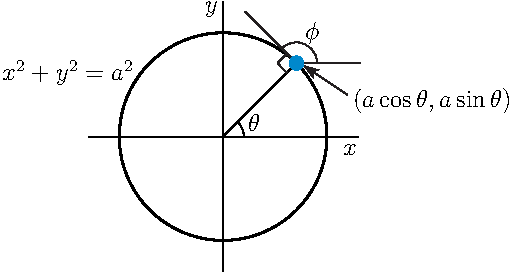
\includegraphics{parCirclePhi.pdf}\quad
       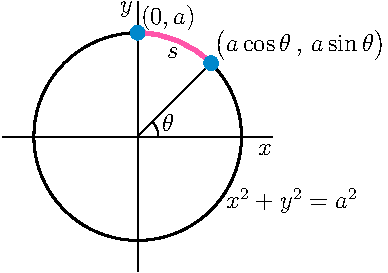
\includegraphics{parCircleS.pdf}
\end{center}


(c) Let $\theta$ be the angle between 
\begin{itemize}\itemsep1pt \parskip0pt \parsep0pt
\item the radius vector from the origin to the point 
$(a\cos\theta,a\sin\theta)$  on the circle and 
\item
the positive $x$-axis. 
\end{itemize} 
The arc from $(0,a)$ to $(a\cos\theta,a\sin\theta)$ 
subtends an angle $\frac{\pi}{2}-\theta$ and so
has length $s=a\big(\frac{\pi}{2}-\theta\big)$. (See the figure
on the right above.) Thus $\theta=\frac{\pi}{2}-\frac{s}{a}$
and the desired parametrization is
\begin{equation*}
\big(x(s),y(s)\big)
=\left(a\cos\left(\frac{\pi}{2}-\frac{s}{a}\right)\,,\,
           a\sin\left(\frac{\pi}{2}-\frac{s}{a}\right)\right)
,\ 0\le s\le\frac{\pi}{2}a
\end{equation*}
\end{solution}





%%%%%%%%%%%%%%%%%%%
\begin{question}
Consider the following time-parametrized curve:
\[\vr(t)=\left( \cos\left(\frac{\pi}{4}t\right)~,~(t-5)^2\right)\]

List the three points $(-1/\sqrt{2},0)$, $(1,25)$, and $(0,25)$ in chronological order.
\end{question}
\begin{hint}
Find the value of $t$ at which the three points occur on the curve.
\end{hint}
\begin{answer}
$(1,25)$, $(-1/\sqrt2,0)$, $(0,25)$.
\end{answer}
\begin{solution}
We can find the time at which the curve hits a given point by considering the two equations that arise from the two coordinates. For the $y$-coordinate to be 0, we must have $(t-5)^2=0$, i.e. $t=5$. So, the point $(-1/\sqrt{2},0)$ happens when $t=5$.

Similarly, for the $y$-coordinate to be $25$,  we need $(t-5)^2=25$, so $(t-5)=\pm 5$.
When $t=0$, the curve hits $(1, 25)$; when $t=10$, the curve hits $(0,25)$.

So, in order, the curve passes through the points $(1,25)$, $(-1/\sqrt2,0)$, and $(0,25)$.
\end{solution}
%%%%%%%%%%%%%%%%%%%
\begin{question}
At what points in the $xy$-plane does the curve $(\sin t, t^2)$ cross itself? What is the difference in $t$ between the first time the curve crosses through a point, and the last?
\end{question}
\begin{hint}
The curve ``crosses itself" when $(\sin t,t^2)$ gives the same coordinate for different values of $t$. When these crossings occur will depend on which crossing you're referring to, so your answers should all depend on $t$.
\end{hint}
\begin{answer}
The curve crosses itself at all points $(0,(\pi n)^2)$ where $n$ is an integer. It passes such a point twice, $2\pi n$ time units apart.
\end{answer}
\begin{solution}
The curve ``crosses itself" when the same coordinates occur for different values of $t$, say $t_1$ and $t_2$. So, we want to know when $\sin t_1=\sin t_2$ and also $t_1^2=t_2^2$. Since $t_1$ and $t_2$ should be different, the second equation tells us $t_2=-t_1$. Then the first equation tells us $\sin t_1=\sin t_2=\sin(-t_1)=-\sin t_1$. That is, $\sin t_1 = -\sin t_1$, so $\sin t_1=0$. That happens whenever $t_1=\pi n$ for an integer $n$.

So, the points at which the curve crosses itself are those points $(0,(\pi n)^2)$ where $n$ is an integer. It passes such a point at times $t=\pi n $ and $t=-\pi n$. So, the curve hits this point $2\pi n$ time units apart.
\end{solution}
%%%%%%%%%%%%%%%%%%%%%%%%%%%%%%%%%%%%%%
\begin{question}\label{prob_s1.1_cycloid}

\begin{center}
\begin{tikzpicture}
\YEaaxis{1}{13}{.5}{3}
\YExcoord{1}{a}
\YEycoord{1}{a}
\draw[thick] (1,2) node[red,vertex, label=above:{\textcolor{red}{$P$}}]{} arc (90:450:1cm);
\foreach \x in {0,1,2,3,4}{
	\MULTIPLY{\x}{.2}{\y}
	\SUBTRACT{1}{\y}{\o}
	\MULTIPLY{\x}{2.25}{\z}
	\MULTIPLY{\z}{57.3}{\zrad}
	\draw[red,opacity=\o] ({1+\z+sin(\zrad)},{1+cos(\zrad)}) node[vertex](P\x){};
	\draw[opacity=\o] ({1+\z},1) node[shape=circle, draw, minimum size=2cm]{}--(P\x);
		}
%\draw[thick, opacity=0.75] (1,2) node[red,vertex, label=above:{\textcolor{red}{$P$}}]{} arc (90:450:1cm);
\draw[red] plot[smooth,domain=0:13]({1+\x+sin(\x r)},{1+cos(\x r)});
\end{tikzpicture}
\end{center}

A circle of radius $a$ rolls along the $x$-axis in the positive direction, starting with its centre at $(a,a)$. In that position, we mark the topmost point on the circle $P$. As the circle moves, $P$ moves with it. Let $\theta$ be  the angle the circle has rolled --- see the diagram below.
\begin{enumerate}[(a)]
\item Give the position of the centre of the circle as a function of $\theta$.
\item Give the position of $P$ as a function of $\theta$.
\end{enumerate}
\begin{center}
\begin{tikzpicture}
\draw[thick] (0,0) node[shape=circle, minimum size=4cm, draw]{};
\draw (1.4,1.4)--(0,0)--(0,2);
\draw[red] (1.4,1.4) node[vertex, label= right:$P$](P){};
\draw[] (0,1) arc (90:45:1cm) node[midway, above]{$\theta$};
\draw[->] (0,2.5) arc(90:45:2.5cm);
\end{tikzpicture}
\end{center}

\end{question}
\begin{hint}
For part (b), find the position of $P$ relative to the centre of the circle. Then combine your answer with part (a).
\end{hint}
\begin{answer}
(a) $(a+a\theta,a)$\qquad
(b)$(a+a\theta+a\sin\theta,a+a\cos\theta)$
\end{answer}
\begin{solution} (a)
Pretend that the circle is a spool of thread. As the 
           circle rolls, it dispenses the thread along the ground.
           When the circle rolls $\theta$ radians, it dispenses the
           arc length $\theta a$ of thread and the circle advances
           a distance $\theta a$. So the centre of the circle has 
           moved $\theta a$ units to the right from its starting point, $x=a$. The centre of the circle always has $y$-coordinate $a$. So, after rolling $\theta$ radians, the centre of the circle is at position $\vc(\theta)=(a+a\theta,a)$.

(b) 
Now, let's consider the position of $P$ on the circle, after the circle has rolled $\theta$ radians. 

\begin{center}
\begin{tikzpicture}
\draw[thick] (0,0) node[shape=circle, minimum size=8cm, draw]{};
\draw (2.8,2.8)--(0,0)--(0,4);
\draw[red] (2.8,2.8) node[vertex, label=above right:$P$](P){};
\draw[] (0,1) arc (90:45:1cm) node[midway, above]{$\theta$};
\draw[dashed] (P)--(0,2.8) node[midway, above]{$a\sin\theta$};
\draw[decorate, decoration={brace, amplitude=10pt}](-.25,0)--(-.25,2.8) node[midway,rotate=90,yshift=7.5mm]{$a\cos\theta$};
\draw[->] (0,5) arc(90:45:5cm);
\end{tikzpicture}
\end{center}
From the diagram, we see that $P$ is $a\cos \theta$ units above the centre of the circle, and $a\sin \theta$ units to the right of it. So, the position of $P$ is $(a+a\theta+a\sin\theta,a+a\cos\theta)$.

Remark: this type of curve is known as a \emph{cycloid}.
\end{solution}
%%%%%%%%%%%%%%%%%%%
\begin{question}\label{prob_s1.0last}
The curve $C$ is defined to be the intersection of the hyperboloid
\[x^2-\frac{1}{4}y^2+3z^2=1\]
and the plane
\[x+y+z=0.\]
When $y$ is very close to 0, and $z$ is negative, find an expression giving $z$ in terms of $y$.
\end{question}
\begin{hint}
We aren't concerned with $x$, so we can eliminate it by solving one equation for $x$ as a function
        of $y$ and $z$ and plugging the result into the other equation.
        \end{hint}
\begin{answer}
$z=-\frac12\sqrt{1-\frac{y^2}{2}}-\frac{y}{4}$
\end{answer}
\begin{solution}
We aren't concerned with $x$, so we can eliminate it by solving for it in one equation, and plugging that into the other. Since $C$ lies on the plane, $x=-y-z$, so:
\begin{align*}
1&=x^2-\frac{1}{4}y^2+3z^2=(-y-z)^2-\frac14y^2+3z^2\\
&=\frac{3}{4}y^2+4z^2+2yz
\intertext{Completing the square,}
1&=\frac{1}{2}y^2+\left(2z+\frac{y}{2}\right)^2\\
1-\frac{y^2}{2}&=\left(2z+\frac{y}{2}\right)^2
\intertext{Since $y$ is small, the left hand is close to $1$
         and the right hand side is close to $(2z)^2$.
         So $(2z)^2\approx 1$. Since $z$ is negative,
         $z\approx -\frac{1}{2}$ and  $2z+\frac{y}{2}<0$. Also, $1-\frac{y^2}{2}$ is positive, so it has a real square root.}
-\sqrt{1-\frac{y^2}{2}}&=2z+\frac{y}{2}\\
-\frac12\sqrt{1-\frac{y^2}{2}}-\frac{y}{4}&=z
\end{align*}

\end{solution}
%%%%%%%%%%%%%%%%%%%
\begin{question}
A particle traces out a curve in space, so that its position at time $t$ is \[\vr(t)=e^{-t}\,\hi+\frac{1}{t}\,\hj+(t-1)^2(t-3)^2\,\hk\] for $t > 0$. 

Let the positive $z$ axis point vertically upwards, as usual. When is the particle moving upwards, and when is it moving downwards? Is it moving faster at time $t=1$ or at time $t=3$?
\end{question}
\begin{hint}
To determine whether the particle is rising or falling, we only need to consider its $z$-coordinate. 
\end{hint}
\begin{answer}
The particle is moving upwards from $t=1$ to $t=2$, and from $t=3$ onwards.  The particle is moving downwards from $t=0$ to $t=1$, and from $t=2$ to $t=3$.

The particle is moving faster when $t=1$ than when $t=3$.
\end{answer}
\begin{solution}
To determine whether the particle is rising or falling, we only need to consider its $z$-coordinate: $z(t)=(t-1)^2(t-3)^2$. Its derivative with respect to time is $z'(t)=4(t-1)(t-2)(t-3)$. This is positive when $1<t<2$ and when $3<t$, so the particle is increasing on $(1,2) \cup (3,\infty)$ and decreasing on $(0,1) \cup (2,3)$.

If $\vr(t)$ is the position of the particle at time $t$, then its speed is $|\vr'(t)|$. We differentiate:
\[\vr'(t)=-e^{-t}\,\hi-\frac{1}{t^2}\,\hj+4(t-1)(t-2)(t-3)\hk\]
So, $\vr(1)=-\frac{1}{e}\,\hi-1\,\hj$ and $\vr(3)=-\frac{1}{e^3}\,\hi-\frac{1}{9}\,\hj$. The absolute value of every component of $\vr(1)$ is greater than or equal to that of the corresponding component of $\vr(3)$, so $|\vr(1)|>|\vr(3)|$. That is, the particle is moving more swiftly at $t=1$ than at $t=3$.

Note: We could also compute the sizes of both vectors directly: $|\vr'(1)|=\sqrt{\left(\frac{1}{e}\right)^2+(-1)^2}$, and $|\vr'(3)|=\sqrt{\left(\frac{1}{e^3}\right)^2+\left(-\frac{1}{9}\right)^2}$.
\end{solution}
%%%%%%%%%%%%%%%%%%%
\begin{question}
Below is the graph of the parametrized function $\vr(t)$. Let $s(t)$ be the arclength along the curve from $\vr(0)$ to $\vr(t)$.

\begin{center}
\begin{tikzpicture}
\draw[thick] plot[domain=-4.5:1]({4-\x*\x/4},\x);
\draw (4-1/16,-.5) node[vertex, label=right: $\vr(t+h)$](th){};
\draw (3,-2) node[vertex, label=right: $\vr(t)$](t){};
\draw (0,-4) node[vertex, label=below right: $\vr(0)$](zero){};
%\draw[|-|, red,yshift=10mm, xshift=-10mm] plot[domain=-4:-2]({4-\x*\x/4},\x);
%\draw[|-|, red,yshift=7.5mm, xshift=-7.5mm] plot[domain=-4:-.5]({4-\x*\x/4},\x);
%\draw[|-|, red,yshift=5mm, xshift=-5mm] plot[domain=-2:-.5]({4-\x*\x/4},\x);
%\draw[very thick, red, ->] (t)--(th);
\end{tikzpicture}
\end{center}
Indicate on the graph $s(t+h)-s(t)$ and $\vr(t+h)-\vr(t)$. Are the quantities scalars or vectors?

%Label $s(t)$, $s(t+h)$, $s(t+h)-s(t)$, and $\vr(t+h)-\vr(t)$. Which are scalars, and which are vectors?

%Lemma 1.1.3: draw a diagram, have students label $h$, $s(t+h)-s(t)$ etc.; which are constants, and which are vectors?
\end{question}
\begin{hint}
This is the setup from Lemma~\eref{CLP317}{lem:CVtanArclen} in the CLP-4. 
The two quantities you're labelling are related, but different.
\end{hint}
\begin{answer}

\begin{center}
\begin{tikzpicture}
\draw[thick] plot[domain=-4.5:1]({4-\x*\x/4},\x);
\draw (4-1/16,-.5) node[vertex, label=right: $\vr(t+h)$](th){};
\draw (3,-2) node[vertex, label=right: $\vr(t)$](t){};
\draw (0,-4) node[vertex, label=below right: $\vr(0)$](zero){};
%\draw[|-|, red,yshift=10mm, xshift=-10mm] plot[domain=-4:-2]({4-\x*\x/4},\x);
%\draw[|-|, red,yshift=7.5mm, xshift=-7.5mm] plot[domain=-4:-.5]({4-\x*\x/4},\x);
\draw[|-|, blue,yshift=-5mm, xshift=10mm] plot[domain=-2:-.5]({4-\x*\x/4},\x);
\draw[very thick, red, ->] (t)--(th);% node[midway, left]{$\vr(t+h)-\vr(t)$};
\end{tikzpicture}
\end{center}
The red vector is $\vr(t+h)-\vr(t)$. The arclength of the segment indicated by the blue line is the (scalar) $s(t+h)-s(t)$.

Remark: as $h$ approaches 0, the curve (if it's differentiable at $t$) starts to resemble a straight line, with the length of the vector $\vr(t+h)-\vr(t)$ approaching the scalar $s(t+h)-s(t)$. This step is crucial to understanding Lemma~\eref{CLP317}{lem:CVtanArclen} in the CLP-4 text. 
\end{answer}
\begin{solution}

\begin{center}
\begin{tikzpicture}
\draw[thick] plot[domain=-4.5:1]({4-\x*\x/4},\x);
\draw (4-1/16,-.5) node[vertex, label=right: $\vr(t+h)$](th){};
\draw (3,-2) node[vertex, label=right: $\vr(t)$](t){};
\draw (0,-4) node[vertex, label=below right: $\vr(0)$](zero){};
%\draw[|-|, red,yshift=10mm, xshift=-10mm] plot[domain=-4:-2]({4-\x*\x/4},\x);
%\draw[|-|, red,yshift=7.5mm, xshift=-7.5mm] plot[domain=-4:-.5]({4-\x*\x/4},\x);
\draw[|-|, blue,yshift=-5mm, xshift=10mm] plot[domain=-2:-.5]({4-\x*\x/4},\x);
\draw[very thick, red, ->] (t)--(th);% node[midway, left]{$\vr(t+h)-\vr(t)$};
\end{tikzpicture}
\end{center}
The red vector is $\vr(t+h)-\vr(t)$. The arclength of the segment indicated by the blue line is the (scalar) $s(t+h)-s(t)$.

Remark: as $h$ approaches 0, the curve (if it's differentiable at $t$) starts to resemble a straight line, with the length of the vector $\vr(t+h)-\vr(t)$ approaching the scalar $s(t+h)-s(t)$. This step is crucial to understanding Lemma~\eref{CLP317}{lem:CVtanArclen}  in the CLP-4 text. 

\end{solution}
%%%%%%%%%%%%%%%%%%%
%%%%%%%%%%%%%%%%%%%
\begin{question}
What is the relationship between velocity and speed in a vector-valued function of time?
\end{question}
\begin{hint} See the note just before Example~\eref{CLP317}{eg:paramCircleTan}.
\end{hint}
\begin{answer}
Velocity is a vector-valued quantity, so it has both a magnitude and a direction. Speed is a scalar --- the magnitude of the velocity. It does not include a direction.
\end{answer}
\begin{solution}
Velocity is a vector-valued quantity, so it has both a magnitude and a direction. Speed is a scalar --- the magnitude of the velocity. It does not include a direction.
\end{solution}
%%%%%%%%%%%%%%%%%%%

%%%%%%%%%%%%%%%%%%%
\begin{question}[M317 2005D] %1
Let $\vr(t)$ be a vector valued function. Let $\vr'$, $\vr''$ , and $\vr'''$ 
denote $\diff{\vr}{t}$, $\difftwo{\vr}{t}$ and 
$\frac{\mathrm{d^3}\hfil\vr\hfil}{\mathrm{d}{t}^3}$, respectively.
Express
\begin{equation*}
\diff{\hfill}{t}\big[ (\vr \times \vr')\cdot\vr'' \big]
\end{equation*}
in terms of $\vr$, $\vr'$ , $\vr''$ , and $\vr'''$. 
Select the correct answer.
\begin{enumerate}[(a)]
\item\ \  $(\vr'\times\vr'' )\cdot\vr'''$
\item\ \  $(\vr'\times\vr'' )\cdot\vr + (\vr\times\vr' )\cdot\vr'''$
\item\ \  $(\vr\times\vr' )\cdot\vr'''$
\item\ \  $0$
\item\ \  None of the above.
\end{enumerate}
\end{question}

\begin{hint} 
To simplify your answer, remember: the cross product of $\va$ and $\vb$ is a vector orthogonal to both $\va$ and $\vb$; the cross product of a vector with itself is zero; and two orthogonal vectors have dot product 0.
\end{hint}

\begin{answer} 
(c)
\end{answer}

\begin{solution}
By the product rule
\begin{align*}
\diff{\hfill}{t}\big[ (\vr \times \vr')\cdot\vr'' \big]
&= (\vr' \times \vr')\cdot\vr''
  +(\vr \times \vr'')\cdot\vr''
  +(\vr \times \vr')\cdot\vr'''
\end{align*}
The first term vanishes because $\vr'\times\vr'=\vZero$.
The second term vanishes because $\vr \times \vr''$ is perpendicular to
$\vr''$. So
\begin{equation*}
\diff{\hfill}{t}\big[ (\vr \times \vr')\cdot\vr'' \big]
= (\vr \times \vr')\cdot\vr'''
\end{equation*}
which is (c).
\end{solution}

%%%%%%%%%%%%%%%%%%%
\begin{question}
Show that, if the position and velocity vectors of a moving 
particle are always perpendicular, then the path of the particle lies on
a sphere.
\end{question}

\begin{hint} 
Evaluate $\diff{}{t} |\vr(t)|^2$.
\end{hint}

\begin{answer}
See the solution.
\end{answer}

\begin{solution}
we are told that $\vr(t)\perp\vr'(t)$, so that $\vr(t)\cdot\vr'(t)=0$, 
for all $t$. Consequently
$$
\diff{}{t}|\vr(t)|^2
=\diff{}{t}\big[\vr(t)\cdot\vr(t)\big]
=2\vr(t)\cdot\vr'(t)=0
$$
So $|\vr(t)|^2$ is a constant, say $A$, independent of time and $\vr(t)$
always lies on the sphere of radius $\sqrt{A}$ centred on the origin.
\end{solution}

%%%%%%%%%%%%%%%%%%
\subsection*{\Procedural}
%%%%%%%%%%%%%%%%%%

%%%%%%%%%%%%%%%%%%%%%%%%%%%
\begin{question}[M317 2005D] %3
Find the speed of a particle with the given position function
\begin{equation*}
\vr(t) = 5 \sqrt{2}\,t\,\hi + e^{5t}\,\hj - e^{-5t}\,\hk
\end{equation*}
Select the correct answer:
\begin{enumerate}[(a)]
\item\ \ 
$|\vv(t)| = \big(e^{5t} + e^{-5t}\big)$
\item\ \ 
$|\vv(t)| = \sqrt{10 + 5e^{t} + 5e^{-t}}$
\item\ \ 
$|\vv(t)| = \sqrt{10 + e^{10t} + e^{-10t}}$
\item\ \ 
$|\vv(t)| = 5\big(e^{5t} + e^{-5t}\big)$
\item\ \ 
$|\vv(t)| = 5\big(e^t + e^{-t}\big)$
\end{enumerate}
\end{question}

\begin{hint} 
Just compute $|\vv(t)|$. Note that $\big(e^{at}+e^{-at}\big)^2 
=e^{2at} + 2 + e^{-2at}$.
\end{hint}

\begin{answer} 
(d)
\end{answer}

\begin{solution}
We have
\begin{equation*}
\vv(t) = \vr'(t) 
      = 5 \sqrt{2}\,\hi + 5e^{5t}\,\hj +5 e^{-5t}\,\hk
\end{equation*}
and hence
\begin{equation*}
|\vv(t)| = |\vr'(t)| 
         = 5 \big|\sqrt{2}\,\hi + e^{5t}\,\hj + e^{-5t}\,\hk\big|
         = 5\sqrt{2+ e^{10t}+ e^{-10t}}
\end{equation*}
Since $2+ e^{10t}+ e^{-10t} = \big(e^{5t}+e^{-5t}\big)^2$, that's (d).
\end{solution}

%%%%%%%%%%%%%%%%%%%%%%%%%%%%%%%
\begin{question}
Find the velocity, speed and acceleration at time $t$ of
the particle whose position is 
\begin{equation*}
\vr(t)= a \cos t\,\hi+a\sin t\,\hj+ct\,\hk
\end{equation*}
Describe the path of the particle.
\end{question}

\begin{hint} 
To figure out what the path looks like, first concentrate on the $x$- and
$y$-coordinates.
\end{hint}

\begin{answer} 
$\text{velocity}=-a \sin t\,\hi+a\cos t\,\hj+c\,\hk$\qquad
$\text{speed}= \sqrt{a^2+c^2}$\qquad
$\text{acceleration}=-a \cos t\,\hi-a\sin t\,\hj$

The path is a helix with radius $a$ and with each turn having height $2\pi c$.
\end{answer}

\begin{solution} 
We are told that
\begin{equation*}
\vr(t)= a \cos t\,\hi+a\sin t\,\hj+ct\,\hk
\end{equation*}
So, by definition,
\begin{align*}
\text{velocity}&= \vv(t)= \vr'(t)=-a \sin t\,\hi+a\cos t\,\hj+c\,\hk\\
\text{speed}&=\diff{s}{t}(t) = |\vr'(t)| = \sqrt{a^2+c^2} \\
\text{acceleration}&=\va(t)= \vr''(t)=-a \cos t\,\hi-a\sin t\,\hj
\end{align*}
As $t$ runs over an interval of length $2\pi$, $(x,y)$ traces
out a circle of radius $a$ and $z$ increases by $2\pi c$.
The path is a helix with radius $a$ and with each turn having height $2\pi c$.
\end{solution}


%%%%%%%%%%%%%%%%%%%
\begin{question}[M317 2013D] %2

\begin{enumerate}[(a)]
\item
Let
\begin{equation*}
\vr(t) = \left(t^2 , 3, \tfrac{1}{3} t^3 \right) 
\end{equation*}
Find the unit tangent vector to this parametrized curve at $t = 1$, 
pointing in the direction of increasing $t$.
\item
Find the arc length of the curve from (a) between the points $(0, 3, 0)$ 
and $(1, 3, -\frac{1}{3})$.

\end{enumerate}
\end{question}

\begin{hint} 
Review \S\eref{CLP317}{sec:CurveCompendium} of the CLP-4 text.
The arc length should be positive.
\end{hint}

\begin{answer} 
(a) $\hat\vT(1) = \frac{(2,0,1)}{\sqrt{5}}$\qquad
(b) $\frac{1}{3}\big[5^{3/2}-8\big]$
\end{answer}

\begin{solution} (a)
Since $\vr'(t) = (2t,0,t^2)$, the specified unit tangent at $t=1$ is
\begin{equation*}
\hat\vT(1) = \frac{(2,0,1)}{\sqrt{5}}
\end{equation*}

\noindent (b)
We are to find the arc length between $\vr(0)$ and $\vr(-1)$. 
As $\diff{s}{t}=\sqrt{4t^2+t^4}$, the 
\begin{align*}
\text{arc length} &= \int_{-1}^0 \sqrt{4t^2+t^4}\ \dee{t}
\end{align*}
The integrand is even, so
\begin{align*}
\text{arc length} &= \int_0^1 \sqrt{4t^2+t^4}\ \dee{t}
=\int_0^1 t\sqrt{4+t^2}\ \dee{t}
=\Big[\tfrac{1}{3}{(4+t^2)}^{3/2}\Big]_0^1
=\tfrac{1}{3}\big[5^{3/2}-8\big]
\end{align*}

\end{solution}



%%%%%%%%%%%%%%%%%%%
\begin{question}\label{prob_s1.1:lemma113}
Using Lemma~\eref{CLP317}{lem:CVtanArclen}  in the CLP-4 text, 
find the arclength of $\vr(t)=\left(t,\sqrt{\frac{3}{2}}t^2,t^3\right)$ 
from $t=0$ to $t=1$.
\end{question}
\begin{hint}
From Lemma~\eref{CLP317}{lem:CVtanArclen} in the CLP-4 text, we know 
the arclength from $t=0$ to $t=1$ will be
\[\int_{0}^1\left| \diff{\vr}{t}(t)\right|\dee t\]
The notation looks a little confusing at first, but we can break it down piece by piece: $\diff{\vr}{t}(t)$ is a vector, whose components are functions of $t$. If we take its magnitude, we'll get one big function of $t$. That function is what we integrate. Before integrating it, however, we should simplify as much as possible.
\end{hint}
\begin{answer}
2
\end{answer}
\begin{solution}
By Lemma~\eref{CLP317}{lem:CVtanArclen}  in the CLP-4 text,  
the arclength of $\vr(t)$ from $t=0$ to $t=1$ is
$\int_{0}^1\left| \diff{\vr}{t}(t)\right|\dee t$. We'll calculate this in a few pieces to make the steps clearer.
\begin{align*}
\vr(t)&=\left(t,\sqrt{\frac{3}{2}}t^2,t^3\right)\\
\diff{\vr}{t}(t)&=\left(1,\sqrt{6}t,3t^2\right)\\
\left|\diff{\vr}{t}(t)\right|&=\sqrt{1^2+(\sqrt{6}t)^2+(3t^2)^2}=\sqrt{1+6t^2+9t^4}=\sqrt{(3t^2+1)^2}=3t^2+1\\
\int_{0}^1\left| \diff{\vr}{t}(t)\right|\dee t&=\int_0^1\left(3t^2+1 \right)\dee t=2
\end{align*}
\end{solution}
%%%%%%%%%%%%%%%%%%%


%%%%%%%%%%%%%%%%%%%%%%%%%%%%%%%
\begin{question}
Find the length of the parametric curve
\begin{equation*}
x=a\cos t\sin t\qquad
y=a\sin^2 t\qquad
z=bt
\end{equation*}
between $t=0$ and $t=T>0$.
\end{question}

%\begin{hint} 
%
%\end{hint}

\begin{answer} 
$\text{length}=\sqrt{a^2+b^2}\,T$
\end{answer}

\begin{solution} 
Since
\begin{align*}
x'(t)&=a\big[\cos^2 t-\sin^2 t\big]=a\cos 2t\\
y'(t)&=2a\sin t\cos t=a\sin 2t\\
z'(t)&=b
\end{align*}
we have
\begin{equation*}
\diff{s}{t}(t)
=\sqrt{x'(t)^2+y'(t)^2+z'(t)^2}=\sqrt{a^2+b^2}
\end{equation*}
As the speed $\diff{s}{t}(t)$ is constant, the length is just
$\diff{s}{t}\,T=\sqrt{a^2+b^2}\,T$.

\end{solution}


%%%%%%%%%%%%%%%%%%%%%%%%%%%%%%%%%%%%%%
\begin{question}
A particle's position at time $t$ is given by $\vr(t)=(t+\sin t, \cos t)$\footnote{The particle traces out a cycloid --- see Question~\ref{prob_s1.1_cycloid}}. What is the magnitude of the acceleration of the particle at time $t$?
\end{question}
\begin{hint}
$\vr(t)$ is the position of the particle, so its acceleration is $r''(t)$.
\end{hint}
\begin{answer}
1
\end{answer}
\begin{solution}
Since $\vr(t)$ is the position of the particle,  its acceleration is $r''(t)$.
\begin{align*}
\vr(t)&=(t+\sin t, \cos t)\\
\vr'(t)&=(1+\cos t,-\sin t)\\
\vr''(t)&=(-\sin t,-\cos t)\\
|\vr''(t)|&=\sqrt{\sin^2t+\cos^2t}=1
\end{align*}
The magnitude of acceleration is constant, but its \emph{direction} is changing, since $\vr''(t)$ is a vector with changing direction.
\end{solution}



%%%%%%%%%%%%%%%%%%%%%%%%%%%
\begin{question}[M317 2011D] %2
A curve in $\bbbr^3$ is given by the vector equation 
$\vr(t) = \left(2t \cos t, 2t \sin t,\frac{t^3}{3}\right)$

\begin{enumerate}[(a)]
\item
Find the length of the curve between $t = 0$ and $t = 2$.

\item
Find the parametric equations of the tangent line to the curve at $t = \pi$.

\end{enumerate}
\end{question}

\begin{hint} 
Review \S\eref{CLP317}{sec:CurveCompendium} of the CLP-4 text.
\end{hint}

\begin{answer} 
(a) $\nicefrac{20}{3}$\qquad
(b) $x(t) = -2\pi -2t,\ 
     y(t) =  -2\pi t,\ 
     z(t) = \nicefrac{\pi^3}{3} + \pi^2 t$ 
\end{answer}

\begin{solution} (a) The speed is
\begin{align*}
\diff{s}{t}(t)
=\big|\vr'(t)\big| & = \left|\left(2\cos t - 2t\sin t\,,\,
                                  2\sin t + 2t \cos t\,,\,
                                  t^2\right)\right| \\
                  &=\sqrt{\big(2\cos t - 2t\sin t\big)^2
                         +\big(2\sin t + 2t \cos t\big)^2
                         +t^4} \\
                 &= \sqrt{4+ 4t^2 +t^4} \\
                 &= 2+t^2
\end{align*}
so the length of the curve is
\begin{align*}
\text{length }
&=\int_0^2 \diff{s}{t}\,\dee{t}
  =\int_0^2 (2+t^2)\,\dee{t}
  = \left[2t +\frac{t^3}{3}\right]_0^2
  =\frac{20}{3}
\end{align*}

\noindent (b)
A tangent vector to the curve at 
$\vr(\pi)=\big(-2\pi\,,\, 0\,,\, \nicefrac{\pi^3}{3}\big)$ is
\begin{equation*}
\vr'(\pi) = \left(2\cos\pi - 2\pi\sin\pi\,,\,
                                  2\sin\pi + 2\pi \cos\pi\,,\,
                                  \pi^2\right)
 = (-2\,,\,-2\pi\,,\,\pi^2)
\end{equation*}
So parametric equations for the tangent line at $\vr(\pi)$ are
\begin{align*}
x(t) &= -2\pi -2t \\
y(t) &=  -2\pi t \\
z(t) &= \nicefrac{\pi^3}{3} + \pi^2 t 
\end{align*}
\end{solution}
%%%%%%%%%%%%%%%%%%%%%%%%%%%%%%%

\begin{question}[M317 2010D]  %1
Let $\vr(t) = \big(3 \cos t, 3 \sin t, 4t\big)$ be the position vector 
of a particle as a function of time $t \ge 0$.
\begin{enumerate}[(a)]
\item
Find the velocity of the particle as a function of time $t$.
\item
Find the arclength of its path between $t = 1$ and $t = 2$.
\end{enumerate}
\end{question}

\begin{hint} 
Review \S\eref{CLP317}{sec curve derivs} of the CLP-4 text.
\end{hint}

\begin{answer} 
(a) $\vr'(t) = \big(-3 \sin t, 3 \cos t, 4\big)$\qquad
(b) 5
\end{answer}

\begin{solution} (a) As $\vr(t) = \big(3 \cos t, 3 \sin t, 4t\big)$,
the velocity of the particle is
\begin{equation*}
\vr'(t) = \big(-3 \sin t, 3 \cos t, 4\big)
\end{equation*}

\noindent (b) As $\diff{s}{t}$, the rate of change of arc length per unit time,
is
\begin{equation*}
\diff{s}{t}(t) = |\vr'(t)| = \big|\big(-3 \sin t, 3 \cos t, 4\big)\big|
  =5
\end{equation*}
the arclength of its path between $t = 1$ and $t = 2$ is
\begin{equation*}
\int_1^2\dee{t}\ \diff{s}{t}(t) 
=\int_1^2\dee{t}\ 5
=5
\end{equation*}
\end{solution}

%%%%%%%%%%%%%%%%%%%%%%%%%%%%%%%
\begin{question}
The plane $\ z=2x+3y\ $ intersects the cylinder 
$\ x^2+y^2=9\ $ in an ellipse. 
\begin{enumerate}[(a)]
\item
Find a parametrization of the ellipse. 
\item
Express the circumference of this ellipse as an integral. 
You need not evaluate the integral\footnote{The indefinite integral involved is one of a class of integrals called elliptic integrals because of their connections to arc lengths of ellipses. In general, elliptic integrals cannot be expressed in terms of elementary functions. You can easily find discussions of elliptic integrals using your favourite search engine.}.
\end{enumerate}
\end{question}

\begin{hint} 
(a) First parametrize $x^2+y^2=9$.
\end{hint}

\begin{answer} 
(a) $x(\theta)=3\cos\theta,\ 
y(\theta)=3\sin\theta,\ 
z(\theta)=6\cos\theta+9\sin\theta,\ 
0\le\theta\le 2\pi$

(b) $s=\int_0^{2\pi} \sqrt{45+45\cos^2\theta-108\sin\theta\cos\theta}\,d\theta$

\end{answer}

\begin{solution} (a)
We can parametrize the circle  $\ x^2+y^2=9\ $ as 
$x(\theta)=3\cos\theta$, $y(\theta)=3\sin\theta$ with 
$\theta$ running from $0$ to $2\pi$. As $z=2x+3y$, the 
ellipse can be parametrized by
\begin{equation*}
x(\theta)=3\cos\theta,\ 
y(\theta)=3\sin\theta,\ 
z(\theta)=2x(\theta)+3 y(\theta)
        =6\cos\theta+9\sin\theta,\ 
0\le\theta\le 2\pi
\end{equation*}

(b)
As
\begin{align*}
\diff{s}{\theta}
 &=\sqrt{x'(\theta)^2+y'(\theta)^2+z'(\theta)^2}\\
 &=\sqrt{9\sin^2\theta+9\cos^2\theta+36\sin^2\theta
        +81\cos^2\theta-108\sin\theta\cos\theta}\\
&=\sqrt{45+45\cos^2\theta-108\sin\theta\cos\theta}
\end{align*}
the circumference is
\begin{equation*}
s=\int_0^{2\pi} \sqrt{45+45\cos^2\theta-108\sin\theta\cos\theta}\,\dee{\theta}
\end{equation*}
\end{solution}



%%%%%%%%%%%%%%%%%%%%%%%%%%
\begin{question}[M317 2007A] %2
	Consider the curve
	\begin{equation*}
	\vr(t) = \frac{1}{3}\cos^3 t\,\hi +\frac{1}{3} \sin^3 t\,\hj + \sin^3 t\,\hk
	\end{equation*}
	\begin{enumerate}[(a)]
		\item
		Compute the arc length of the curve from $t = 0$ to $t = \frac{\pi}{2}$.
		\item
		Compute the arc length of the curve from $t = 0$ to $t = \pi$.
	\end{enumerate}
\end{question}

\begin{hint} 
	If you got the answer $0$ in part (b), you dropped some absolute value signs.
\end{hint}

\begin{answer} 
	(a) $\frac{1}{27}\big(10\sqrt{10}-1\big)$\qquad
	(b) $\frac{2}{27}\big(10\sqrt{10}-1\big)$
\end{answer}

\begin{solution} (a)
	As
	\begin{align*}
	\vr'(t) & = -\sin t\cos^2 t\,\hi + \sin^2 t\cos t\,\hi + 3\sin^2 t\cos t\,\hk
	= \sin t\cos t\big(-\cos t\,\hi +\sin t\,\hj +3\sin t\,\hk\big) \\
	\diff{s}{t}(t) & = |\sin t\cos t|\sqrt{\cos^2 t + \sin ^2 t + 9\sin^2 t}
	= |\sin t\cos t|\sqrt{1+ 9\sin^2 t}
	\end{align*}
	the arclength from $t = 0$ to $t = \frac{\pi}{2}$ is
	\begin{align*}
	\int_0^{\pi/2} \diff{s}{t}(t)\,\dee{t}
	&=\int_0^{\pi/2} \sin t\cos t \sqrt{1+ 9\sin^2 t}\,\dee{t} \\
	&=\frac{1}{18}\int_1^{10} \sqrt{u}\ \dee{u} \qquad
	\text{with } u = 1+ 9\sin^2 t,\ \dee{u}  = 18\sin t\cos t\,\dee{t}\\
	&=\frac{1}{18}\Big[\frac{2}{3}u^{3/2}\Big]_1^{10}\\
	&=\frac{1}{27}\big(10\sqrt{10}-1\big)
	\end{align*}
	
	(b) The arclength from $t = 0$ to $t = \pi$ is
	\begin{align*}
	\int_0^{\pi} \diff{s}{t}(t)\,\dee{t}
	&=\int_0^{\pi} |\sin t\cos t| \sqrt{1+ 9\sin^2 t}\,\dee{t} 
	\qquad\text{Don't forget the absolute value signs!}\\
	&=2\int_0^{\pi/2} |\sin t\cos t| \sqrt{1+ 9\sin^2 t}\,\dee{t} 
	= 2\int_0^{\pi/2} \sin t\cos t \sqrt{1+ 9\sin^2 t}\,\dee{t} 
	\end{align*}
	since the integrand is invariant under $t\rightarrow\pi-t$. So the arc length
	from $t = 0$ to $t = \pi$ is just twice the arc length from part (a), namely $\frac{2}{27}\big(10\sqrt{10}-1\big)$.
	
\end{solution}
%%%%%%%%%%%%%%%%%%%%%%%%%%%%%%%
\begin{question}[M317 2017D] %2
Let $\vr(t)=\big(\frac{1}{3}t^3,\frac{1}{2}t^2,\frac{1}{2}t\big)$,
$t\ge 0$. Compute $s(t$), the arclength of the curve at time
$t$.
\end{question}

%\begin{hint} 
%\end{hint}

\begin{answer} 
$s(t)=\frac{t^3}{3} +\frac{t}{2}$
\end{answer}

\begin{solution} 
Since
\begin{align*}
\vr(t)&= \frac{t^3}{3}\,\hi + \frac{t^2}{2}\,\hj +  \frac{t}{2}\,\hk\\
\vr'(t)&= t^2\,\hi + t\,\hj + \frac{1}{2}\,\hk \\
\diff{s}{t}(t)=|\vr'(t)|&=\sqrt{t^4+t^2+\frac{1}{4}}
=\sqrt{\Big(t^2+\frac{1}{2}\Big)^2}=t^2+\frac{1}{2}
\end{align*}
the length of the curve is
\begin{align*}
s(t)=\int_0^t \diff{s}{t}(u)\,\dee{u}
=\int_0^t \Big(u^2+\frac{1}{2}\Big)\,\dee{u}
=\frac{t^3}{3} +\frac{t}{2}
\end{align*}
\end{solution}


%%%%%%%%%%%%%%%%%%%%%%%%%%%%%%%
\begin{question}[M317 2011A] %3
Find the arc length of the curve 
$\vr(t) = \big(t^m\,,\, t^m\,,\, t^{3m/2}\big)$ for $0 \le a \le t \le b$, 
and where $m > 0$.
Express your result in terms of $m$, $a$, and $b$. 
\end{question}

\begin{hint} 
The integral you get can be evaluated with
a simple substitution. You may want to factor the integrand first.
\end{hint}

\begin{answer} 
$\frac{8}{27}\Big[\Big(2 + \frac{9}{4}b^m\Big)^{3/2}
                   -\Big(2 + \frac{9}{4}a^m\Big)^{3/2}\Big]$
\end{answer}

\begin{solution} 
Since
\begin{align*}
\vr(t) & = t^m\,\hi + t^m\,\hj + t^{3m/2}\,\hk \\
\vr'(t) &= mt^{m-1}\,\hi + mt^{m-1}\,\hj +\frac{3m}{2}t^{3m/2-1}\,\hk \\
\diff{s}{t} = |\vr'(t)| & = \sqrt{ 2m^2 t^{2m-2} +\frac{9m^2}{4} t^{3m-2} } 
= mt^{m-1}\sqrt{2 + \frac{9}{4}t^m }
\end{align*}
the arc length is
\begin{align*}
\int_a^b \diff{s}{t}(t)\,\dee{t}
&=\int_a^b mt^{m-1}\sqrt{2 + \frac{9}{4}t^m }\ \dee{t} \\
&=\frac{4}{9}\int_{2 + \frac{9}{4}a^m}^{2 + \frac{9}{4}b^m}\sqrt{u}\,\dee{u}
\qquad\text{with } u = 2 + \frac{9}{4}t^m,\ \dee{u} = \frac{9m}{4}t^{m-1}\\
&=\frac{4}{9}\Big[\frac{2}{3}u^{3/2}\Big]_{2 + \frac{9}{4}a^m}
                                         ^{2 + \frac{9}{4}b^m} \\
&=\frac{8}{27}\Big[\Big(2 + \frac{9}{4}b^m\Big)^{3/2}
                   -\Big(2 + \frac{9}{4}a^m\Big)^{3/2}\Big]
\end{align*} 
\end{solution}


%%%%%%%%%%%%%%%%%%%%%%%%%%%%%%%
\begin{question}
 Let $C$ be the part of the curve of intersection of the 
parabolic cylinder $x = y^2$ and the hyperbolic  paraboloid $3z = 2xy$
with $y\ge 0$.
\begin{enumerate}[(a)] 
\item
   Write a vector parametric equation for $C$ using $x$ as the parameter. 
\item 
   Find the length of the part of $C$ between the origin and 
   the point $(9, 3, 18)$. 
\item
   A particle moves along $C$ in the direction for which $x$ is 
   increasing.  If the particle  moves with constant speed 9, find 
   its velocity vector when it is at  the point $(1, 1, \frac{2}{3})$. 
\item
   Find the acceleration vector of the particle of part (c) 
   when it is at  the point $(1, 1, \frac{2}{3})$. 
\end{enumerate}
\end{question}

\begin{hint} 
(b) $\frac{1}{4x}+1+x$ is a perfect square.

(c), (d) Let 
\begin{itemize}\itemsep1pt \parskip0pt \parsep0pt %\itemindent-15pt
\item
  $\vr(x)$ be the position of the particle when its first coordinate is $x$,
\item
 $\vR(t)$ be the position of the particle at time $t$, and 
\item 
  $x(t)$ be the $x$--coordinate of the particle at time $t$.
\end{itemize}
Then $\vR(t) = \vr\big(x(t)\big)$. We are told $|\vR'(t)|=9$ for all $t$.
\end{hint}

\begin{answer} 
(a) $\vr(x)=x\,\hi+\sqrt{x}\,\hj+\frac{2}{3}x^{3/2}\,\hk$\quad
(b) $21$\quad
(c) $6\,\hi+3\,\hj+6\,\hk$\quad
(d) $-6\,\hi-12\,\hj+12\,\hk$
\end{answer}

\begin{solution} 
(a) 
Since $y=\sqrt{x}$ and $z=\frac{2}{3}xy=\frac{2}{3}x^{3/2}$,
\begin{align*}
\vr(x)&=x\,\hi+\sqrt{x}\,\hj+\frac{2}{3}x^{3/2}\,\hk
\end{align*}
For the remaining parts of this problem we will also need
\begin{align*}
\vr'(x)&=\hi+\frac{1}{2\sqrt{x}}\,\hj+\sqrt{x}\,\hk\\
\vr''(x)&=-\frac{1}{4x^{3/2}}\,\hj+\frac{1}{2\sqrt{x}}\,\hk\\
\diff{s}{x}=|\vr'(x)|
&=\sqrt{1+\frac{1}{4x}+x}
=\sqrt{\left(\frac{1}{2\sqrt{x}}+\sqrt{x}\right)^2}
=\frac{1}{2\sqrt{x}}+\sqrt{x}\\
\diff{s}{x}(1)&=\frac{3}{2}
\end{align*}

(b)
\begin{equation*}
\int_C \ ds
=\int_0^9 \diff{s}{x}\ \dee{x}
=\int_0^9 \left(\frac{1}{2\sqrt{x}}+\sqrt{x}\right)\ \dee{x}
=\left[\sqrt{x}+\frac{2}{3}x^{3/2}\right]_0^9
=3+18
=21
\end{equation*}

(c) 
Denote by
\begin{itemize}\itemsep1pt \parskip0pt \parsep0pt %\itemindent-15pt
\item
  $\vr(x)$ the position of the particle when its first coordinate is $x$,
\item
 $\vR(t)$ the position of the particle at time $t$, 
\item 
  $x(t)$ the $x$--coordinate of the particle at time $t$, and
\item 
  $s(x)$ the arc length of the curve from the origin to $\vr(x)$.
\end{itemize}
We are told that $|\vR'(t)|=9$ for all $t$.
So
\begin{align*}
\vR(t)=\vr\big(x(t)\big)&\implies
\vR'(t)=\vr'\big(x(t)\big)\diff{x}{t}(t) \\
&\implies
9=|\vR'(t)|=\diff{s}{x}\big(x(t)\big) \diff{x}{t}(t)
=\left(\frac{1}{2\sqrt{x(t)}}+\sqrt{x(t)}\right)\diff{x}{t}(t)
\end{align*}
In particular, if the particle is at $(1,1,\frac{2}{3})$ at time $0$, then $x(0)=1$
and
\begin{equation*}
9=\left(\frac{1}{2\sqrt{1}}+\sqrt{1}\right)\diff{x}{t}(0)
\implies \diff{x}{t}(0)=6
\end{equation*}
so that
\begin{equation*}
\vR'(0)=\vr'(1)\diff{x}{t}(0)
=\left(\hi+\frac{1}{2}\,\hj+\hk\right)6
=\ 6\,\hi+3\,\hj+6\,\hk
\end{equation*}

(d)
By the product and chain rules,
\begin{equation*}
\vR'(t)=\vr'\big(x(t)\big)\diff{x}{t}(t)\implies
\vR''(t)=\vr''\big(x(t)\big)\left(\diff{x}{t}(t)\right)^2
+\vr'\big(x(t)\big)\difftwo{x}{t}(t)
\end{equation*}
We saw in part (c) that 
$9=|\vR'(t)|=\Big(\frac{1}{2\sqrt{x(t)}}+\sqrt{x(t)}\Big)\diff{x}{t}(t)$
so that 
\begin{equation*}
\diff{x}{t}(t)=9\left(\frac{1}{2\sqrt{x(t)}}+\sqrt{x(t)}\right)^{-1}
\end{equation*}
Differentiating that gives
\begin{equation*}
\frac{d^2x}{dt^2}(t)=-9\left(\frac{1}{2\sqrt{x(t)}}+\sqrt{x(t)}\right)^{-2}
\left(-\frac{1}{4x(t)^{3/2}}+\frac{1}{2\sqrt{x(t)}}\right)\diff{x}{t}(t)
\end{equation*}
In particular, when $t=0$, $x(0)=1$ and $\diff{x}{t}(0)=6$
\begin{equation*}
\difftwo{x}{t}(0)=-9\left(\frac{3}{2}\right)^{-2}
\left(\frac{1}{4}\right)6=-6
\end{equation*}
so
\begin{align*}
\vR''(0)&=\vr''(1)\ \big(6\big)^2+\vr'(1)\big(-6\big)
=36\left(-\frac{1}{4}\,\hj+\frac{1}{2}\,\hk\right)
-6\left(\hi+\frac{1}{2}\,\hj+\hk\right) \\
&=-6\,\hi-12\,\hj+12\,\hk
\end{align*}
\end{solution}




%%%%%%%%%%%%%%%%%%%
\begin{question}
If a particle has constant mass $m$, position $\vr$, and is moving with velocity $\vv$, then its angular momentum is $\vL=m(\vr\times\vv)$. 

For a particle with mass $m=1$ and position function $\vr=(\sin t, \cos t, t)$, find $\left|\diff{\vL}{t} \right|$.

\end{question}
\begin{hint} 
Given the position of a particle, you can find its velocity.
\end{hint}
\begin{answer}
$|t|$
\end{answer}
\begin{solution}
Given the position of the particle, we can find its velocity:
\[\vv(t)=\vr'(t)=(\cos t, -\sin t , 1)\]
Applying the given formula,
\[\vL(t)=\vr \times \vv=(\sin t , \cos t , t) \times (\cos t, -\sin t , 1).\]
\begin{description}
\item[\textbf{Solution 1:}]
We can first compute the cross product, then differentiate:
\begin{align*}
\vL(t)& = (\cos t + t\sin t)\hi + (t\cos t - \sin t)\hj-\hk\\
\vL'(t)&=t\cos t\,\hi -t\sin t\, \hj\\
|\vL'(t)|&=\sqrt{t^2(\sin^2 t + \cos^2 t)}=\sqrt{t^2}=|t|
\end{align*}
\item[\textbf{Solution 2:}]
Using the product rule:
\begin{align*}
\vL'(t)&=\vr'(t)\times \vv(t) + \vr(t) \times \vv'(t)\\
&=\underbrace{\vr'(t)\times \vr'(t)}_{0} + \vr(t) \times \vv'(t)\\
&= (\sin t ,\cos t,t)\times(-\sin t , -\cos t, 0)\\
&=t\cos t\,\hi-t\sin t\,\hj\\
|\vL'(t)|&=\sqrt{t^2\cos^2 t + t^2\sin t^2  }=|t|
\end{align*}
\end{description}
\end{solution}



%%%%%%%%%%%%%%%%%
\subsection*{\Application}
%%%%%%%%%%%%%%%%%


%%%%%%%%%%%%%%%%%%%%%%%%%%%%
\begin{question}[M317 2000A] %1
 A particle moves along the curve $\cC$ of intersection of
the surfaces $z^2=12y$ and $18x=yz$ in the upward direction. When the particle
is at $(1,3,6)$ its velocity $\vv$ and acceleration $\va$ are given by
$$
\vv =6\,\hi+12\,\hj+12\,\hk\qquad
\va = 27\,\hi+30\,\hj+6\,\hk
$$
\begin{enumerate}[(a)]
\item
 Write a vector parametric equation for $\cC$ using 
$u=\frac{z}{6}$ as a parameter.
\item
 Find the length of $\cC$ from $(0,0,0)$ to $(1,3,6)$.
\item
 If $u=u(t)$ is the parameter value for the particle's position
at time $t$, find $\diff{u}{t}$ when the particle is at $(1,3,6)$.
\item
 Find $\difftwo{u}{t}$ when the particle is at $(1,3,6)$.
\end{enumerate}
\end{question}

\begin{hint} 
If $\vr(u)$ is the parametrization of $\cC$ by $u$, then
the position of the particle at time $t$ is $\vR(t) = \vr\big(u(t)\big)$.
\end{hint}

\begin{answer} 
(a)  $\vr(u)=u^3\,\hi+3u^2\,\hj+6u\,\hk$\qquad
(b)  $7$\qquad
(c)  $2$\qquad
(d)  $1$
\end{answer}

\begin{solution}
(a) 
Since $z=6u$, $y=\frac{z^2}{12}=3u^2$ and $x=\frac{yz}{18}=u^3$,
\begin{align*}
\vr(u)&=u^3\,\hi+3u^2\,\hj+6u\,\hk
\end{align*}

(b)
\begin{align*}
\vr'(u)&=3u^2\,\hi+6u\,\hj+6\,\hk\\
\vr''(u)&=6u\,\hi+6\,\hj\\
\diff{s}{u}(u)=|\vr'(u)|
&=\sqrt{9u^4+36u^2+36}=3\big(u^2+2\big)\\
%\diff{s}{u}(1)&=9
\end{align*}


$$
\int_\cC \ ds
=\int_0^1 \diff{s}{u}\ \dee{u}
=\int_0^1 3\big(u^2+2\big)\ \dee{u}
=\big[u^3+6u\big]_0^1
=7
$$

(c) Denote by $\vR(t)$ the position of the particle at time $t$.
Then
$$
\vR(t)=\vr\big(u(t)\big)\implies
\vR'(t)=\vr'\big(u(t)\big)\diff{u}{t}
$$
In particular, if the particle is at $(1,3,6)$ at time $t_1$, then $u(t_1)=1$
and
$$
6\,\hi+12\,\hj+12\,\hk=\vR'(t_1)=\vr'(1)\diff{u}{t}(t_1)
=\big(3\,\hi+6\,\hj+6\,\hk\big)\diff{u}{t}(t_1)
$$
which implies that $\diff{u}{t}(t_1)=2$.

(d) By the product and chain rules,
$$
\vR'(t)=\vr'\big(u(t)\big)\diff{u}{t}\implies
\vR''(t)=\vr''\big(u(t)\big)\Big(\diff{u}{t}\Big)^2
+\vr'\big(u(t)\big)\difftwo{u}{t}
$$
In particular,
\begin{align*}
27\,\hi+30\,\hj+6\,\hk
&=\vR''(t_1)=\vr''(1)\Big(\diff{u}{t}(t_1)\Big)^2
+\vr'\big(1\big)\difftwo{u}{t}(t_1) \\
&=\big(6\,\hi+6\,\hj\big)2^2+\big(3\,\hi+6\,\hj+6\,\hk\big)\difftwo{u}{t}(t_1)
\end{align*}
Simplifying
$$
3\,\hi+6\,\hj+6\,\hk
=\big(3\,\hi+6\,\hj+6\,\hk\big)\difftwo{u}{t}(t_1)
\implies \difftwo{u}{t}(t_1)=1
$$
\end{solution}


%%%%%%%%%%%%%%%%%%%%%%%%%%%
\begin{question}[M317 2008A] %2
A particle of mass $m = 1$ has position $\vr_0 = \frac{1}{2}\,\hk$ 
and velocity $\vv_0 =\frac{\pi^2}{2}\,\hi$ at time $0$.
It moves under a force
\begin{equation*}
\vF(t) = -3t\,\hi + \sin t\,\hj + 2e^{2t}\,\hk.
\end{equation*}
\begin{enumerate}[(a)]
\item
Determine the position $\vr(t)$ of the particle depending on $t$.
\item
At what time after time $t = 0$ does the particle cross the plane 
$x = 0$ for the first time?
\item
What is the velocity of the particle when it crosses the plane $x = 0$ 
in part (b)?
\end{enumerate}
\end{question}

\begin{hint} 
By Newton's law, $\vF=m\va$.
\end{hint}

\begin{answer} 
(a) $\vr(t) = \big(\frac{\pi^2 t}{2}-\frac{t^3}{2}\big)\,\hi + 
              (t- \sin t)\,\hj + \left(\frac{1}{2}e^{2t}-t\right)\,\hk$ \qquad
(b) $t=\pi$ 

(c) $-\pi^2\,\hi +2\,\hj + \big(e^{2\pi}-1\big)\,\hk$
\end{answer}

\begin{solution} (a)
According to Newton,
\begin{equation*}
m\vr''(t) = \vF(t)\qquad\text{so that}\qquad
\vr''(t) = -3t\,\hi + \sin t\,\hj + 2e^{2t}\,\hk
\end{equation*}
Integrating once gives
\begin{align*}
\vr'(t) = -3\frac{t^2}{2}\,\hi - \cos t\,\hj + e^{2t}\,\hk +\vc
\end{align*}
for some constant vector $\vc$. We are told that $\vr'(0)=\vv_0
=\frac{\pi^2}{2}\,\hi$. This forces $\vc=\frac{\pi^2}{2}\,\hi+\hj-\hk$
so that
\begin{align*}
\vr'(t) = \left(\frac{\pi^2}{2}-\frac{3t^2}{2}\right)\,\hi +(1- \cos t)\,\hj + \big(e^{2t}-1\big)\,\hk 
\end{align*}
Integrating a second time gives
\begin{align*}
\vr(t) = \left(\frac{\pi^2 t}{2}-\frac{t^3}{2}\right)\,\hi +(t- \sin t)\,\hj 
 + \left(\frac{1}{2}e^{2t}-t\right)\,\hk  + \vc
\end{align*}
for some (other) constant vector $\vc$.  We are told that $\vr(0)=\vr_0
=\frac{1}{2}\,\hk$. This forces $\vc=\vZero$
so that
\begin{align*}
\vr(t) = \left(\frac{\pi^2 t}{2}-\frac{t^3}{2}\right)\,\hi +(t- \sin t)\,\hj 
 + \left(\frac{1}{2}e^{2t}-t\right)\,\hk 
\end{align*}

(b) The particle is in the plane $x=0$ when
\begin{align*}
0=\left(\frac{\pi^2 t}{2}-\frac{t^3}{2}\right)
 =\frac{t}{2}(\pi^2-t^2) 
\iff t=0, \pm\pi
\end{align*}
So the desired time is $t=\pi$.

(c) At time $t=\pi$, the velocity is
\begin{align*}
\vr'(\pi) 
&= \left(\frac{\pi^2}{2}-\frac{3\pi^2}{2}\right)\,\hi +(1- \cos\pi)\,\hj +                 \big(e^{2\pi}-1\big)\,\hk \\
&= -\pi^2\,\hi +2\,\hj + \big(e^{2\pi}-1\big)\,\hk
\end{align*}

\end{solution}
%%%%%%%%%%%%%%%%%%%%%%%%%%%%
\begin{question}[M317 1999A] %1
 Let $C$ be the curve of intersection of
the surfaces $y=x^2$ and $z=\frac{2}{3}x^3$.
A particle moves along $C$ with constant speed such that $\diff{x}{t}>0$.
The particle is at $(0,0,0)$ at time $t=0$ and is at $(3,9,18)$ at time
$t=\frac{7}{2}$.
\begin{enumerate}[(a)]
\item
Find the length of the part of $C$ between $(0,0,0)$ and $(3,9,18)$.
\item
Find the constant speed of the particle.
\item
Find the velocity of the particle when it is at $\big(1,1,\frac{2}{3}\big)$.
\item
Find the acceleration of the particle when it is at $\big(1,1,\frac{2}{3}\big)$.
\end{enumerate}
\end{question}

\begin{hint} 
Denote by $\vr(x)$ the parametrization of $C$ by $x$. If the $x$-coordinate
of the particle at time $t$ is $x(t)$, then the position of the particle at time $t$ is $\vR(t)=\vr\big(x(t)\big)$. Also, though the particle is moving at a constant speed, it doesn't necessarily have a constant value of $\diff{\vx}{t}$.
\end{hint}

\begin{answer} 
(a) $21$\qquad
(b) $6$\qquad
(c) $2\hi+4\,\hj+4\,\hk$\qquad
(d) $-\frac{8}{3}\big(2\hi+\,\hj-2\,\hk\big)$
\end{answer}

\begin{solution}
(a) Parametrize $C$ by $x$. Since $y=x^2$ and $z=\frac{2}{3}x^3$,
\begin{align*}
\vr(x)&=x\,\hi+x^2\,\hj+\frac{2}{3}x^3\,\hk\\
\vr'(x)&=\hi+2x\,\hj+2x^2\,\hk\\
\vr''(x)&=2\,\hj+4x\,\hk\\
\diff{s}{x}
&=|\vr'(x)|
=\sqrt{1+4x^2+4x^4}=1+2x^2
\end{align*}
and
$$
\int_C \ \dee{s}
=\int_0^3 \diff{s}{x}\ \dee{x}
=\int_0^3 \big(1+2x^2\big)\ \dee{x}
={\Big[x+\frac{2}{3}x^3\Big]}_0^3
=21
$$

(b) The particle travelled a distance of 21 units in $\frac{7}{2}$
time units. This corresponds to a speed of $\frac{21}{7/2}=6$.

(c) Denote by $\vR(t)$ the position of the particle at time $t$.
Then
$$
\vR(t)=\vr\big(x(t)\big)\implies
\vR'(t)=\vr'\big(x(t)\big)\diff{x}{t}
$$
By parts (a) and (b) and the chain rule
$$
6=\diff{s}{t}=\diff{s}{x}\diff{x}{t}=(1+2x^2)\diff{x}{t}
\implies \diff{x}{t}=\frac{6}{1+2x^2}
$$
In particular, the particle is at $\big(1,1,\frac{2}{3}\big)$ at $x=1$.
At this time $\diff{x}{t}=\frac{6}{1+2\times 1}=2$ and
$$
\vR'=\vr'\big(1\big)\diff{x}{t}
=\big(\hi+2\,\hj+2\,\hk\big)2
=2\hi+4\,\hj+4\,\hk
$$

(d) By the product and chain rules,
$$
\vR'(t)=\vr'\big(x(t)\big)\diff{x}{t}\implies
\vR''(t)=\vr''\big(x(t)\big){\Big(\diff{x}{t}\Big)}^2
+\vr'\big(x(t)\big)\difftwo{x}{t}
$$
Applying $\diff{\hfill}{t}$ to $6=\big(1+2x(t)^2\big)\diff{x}{t}(t)$ gives
$$
0=4x{\Big(\diff{x}{t}\Big)}^2+(1+2x^2)\difftwo{x}{t}
$$
In particular, when $x=1$ and $\diff{x}{t}=2$,
 $0=4\times 1\big(2\big)^2+(3)\difftwo{x}{t}$ gives
$\difftwo{x}{t}=-\frac{16}{3}$ and
$$
\vR''=\big(2\,\hj+4\,\hk\big)\big(2\big)^2
-\big(\hi+2\,\hj+2\,\hk\big)\frac{16}{3}
= -\frac{8}{3}\big(2\hi+\,\hj-2\,\hk\big)
$$

\end{solution}







%%%%%%%%%%%%%%%%%%%
\begin{question}
A camera mounted to a pole can swivel around in a full circle. It is tracking an object whose position at time $t$ seconds is $x(t)$ metres east of the pole, and $y(t)$ metres north of the pole.

In order to always be pointing directly at the object, how fast should the camera be programmed to rotate at time $t$? (Give your answer in terms of $x(t)$ and $y(t)$ and their derivatives, in the units rad/sec.)
\end{question}
\begin{hint} 
The question is already set up as an $xy$-plane, with the camera at the origin, so the vector in the direction the camera is pointing is $(x(t),y(t))$. Let $\theta$ be the angle the camera makes with the positive $x$-axis (due east). The tangent function gives a clean-looking relation between $\theta(t)$, $x(t)$, and $y(t)$.
\end{hint}
\begin{answer}
$\frac{x(t)y'(t)-y(t)x'(t)}{x^2+y^2}$
\end{answer}
\begin{solution}
The question is already set up as an $xy$-plane, with the camera at the origin, so the vector in the direction the camera is pointing is $(x(t),y(t))$. Let $\theta$ be the angle the camera makes with the positive $x$-axis (due east). The camera, the object, and the due-east direction (positive $x$-axis) make a right triangle.
\begin{center}
\begin{tikzpicture}
\YEaaxis{.5}{4}{.5}{3}
\draw[thick, ->] (0,0)--(3,2)node[xshift=1mm,yshift=.67mm,vertex, label=right:{object}]{};
\draw (1,0) arc (0:32:10mm) node[midway, right]{$\theta$};
\YExcoord{3}{x(t)}
\YEycoord{2}{y(t)}
\draw (0,0) node[vertex, label=below left:{camera}]{};
\end{tikzpicture}
\end{center}
\begin{align*}
\tan\theta&=\frac{y}{x}\intertext{Differentiating implicitly with respect to $t$:}
\sec^2\theta\,\diff{\theta}{t}&=\frac{xy'-yx'}{x^2}\\
\diff{\theta}{t}&=\cos^2\theta\left(\frac{xy'-yx'}{x^2}\right)=\left(\frac{x}{\sqrt{x^2+y^2}}\right)^2\left(\frac{xy'-yx'}{x^2}\right)=\frac{xy'-yx'}{{x^2+y^2}}
\end{align*}
\end{solution}

%%%%%%%%%%%%%%%%%%%
\begin{question}
A pipe of radius 3 follows the path of the curve $\vr(t)=(\frac{2\sqrt2}{3}t^{3/2}~,~\frac12t^2~,~t+2)$, for $0 \le t \le 10$. 

What is the volume inside the pipe? What is the surface area of the pipe?
\end{question}
\begin{hint}
Usng the Theorem of Pappus, the surface area and volume of this pipe are the same as that of a straight pipe with the same length and radius.
\end{hint}
\begin{answer}
Volume: $540 \pi$ \qquad Surface area: $360\pi$
\end{answer}
\begin{solution}
Using the Theorem of Pappus, we can calculate the surface area and volume of a pipe with the same length and radius as this pipe. So, we need to find the length of the pipe, $L$. 
\begin{align*}
\diff{\vr}{t}&=(\sqrt{2t},t,1)\\
\left| \diff{\vr}{t}\right|&=\sqrt{2t+t^2+1}=|t+1|\\
L&=\int_0^{10}(t+1)\dee{t}=60
\end{align*}

A pipe with radius 3 and length 60 has surface area $60(2\pi\cdot 3)=360\pi$ 
and volume $60(\pi \cdot3^2)=540\pi$.

\end{solution}
%%%%%%%%%%%%%%%%%%%

%%%%%%%%%%%%%%%%%%%
\begin{question}
A wire of total length 1000cm is formed into a flexible coil that is a 
circular helix. If there are 10 turns to each centimetre of height and the 
radius of the helix is 3 cm, how tall is the coil?
\end{question}

\begin{hint} 
A helix can be parametrized by 
$\vr(\theta)=a\cos\theta\,\hi+a\sin\theta\,\hj+b\theta\,\hk$.
\end{hint}

\begin{answer}
$\dfrac{50}{\pi\sqrt{9+\frac{1}{400\pi^2}}}\approx 5.3\textrm{ cm}$
\end{answer}

\begin{solution}
In general a helix can be parametrized by
\begin{equation*}
\vr(\theta)=a\cos\theta\,\hi+a\sin\theta\,\hj+b\theta\,\hk
\end{equation*}
Our first task is to determine $a$ and $b$.
The radius of the helix is $3$ cm, so $a=3$ cm. 
After 10 turns (i.e. $\theta=20\pi$) the height, $b\theta$,
is 1 cm. So $b(20\pi)=1$ and $b=\frac{1}{20\pi}$cm/rad. 
Thus 
$\vr(\theta)=3\cos\theta\,\hi+3\sin\theta\,\hj+\frac{1}{20\pi}\theta\hk$.

With each full turn of the helix (i.e. each increase of $\theta$ by $2\pi$)
the height of the helix increases by $2\pi b=\frac{1}{10}\textrm{cm}$.
So if we can determine the length of wire in one full turn of the helix, 
we can easily determine how many turns the helix goes through in total,
and from that we can determine the total height of the helix.

As $\vr'(\theta)=-3\sin\theta\,\hi+3\cos\theta\,\hj+\frac{1}{20\pi}\hk$
we have $\diff{s}{\theta}=\big|\vr'(\theta)\big|=\sqrt{9+\frac{1}{400\pi^2}}$.
So the length of one full turn of the helix is
\begin{align*}
\int_0^{2\pi}\sqrt{9+\frac{1}{400\pi^2}}\ \dee{\theta}
&=2\pi\sqrt{9+\frac{1}{400\pi^2}}
\end{align*}
and 1000cm of wire generates
\begin{equation*}
\frac{1000}{2\pi\sqrt{9+\frac{1}{400\pi^2}}}
=\frac{500}{\pi\sqrt{9+\frac{1}{400\pi^2}}}
\end{equation*}
turns. Each turn adds $\frac{1}{10}\textrm{cm}$ to the height, so the total height is
\begin{equation*}
\frac{500}{\pi\sqrt{9+\frac{1}{400\pi^2}}}\cdot \frac{1}{10}
=\frac{50}{\pi\sqrt{9+\frac{1}{400\pi^2}}}
\approx 5.3\textrm{ cm}
\end{equation*}

\emph{Remark.} 
We can check that this answer is reasonable by taking advantage of the fact
that each coil adds only a very small height (relative to the radius).
So we expect the length of one coil to be \emph{about} the same as the circumference of a circle of the same radius, namely $6\pi$. 
If we were making actual circles of the wire, there would be $\frac{1000}{6\pi}$ of them. Stacking up at 10 per centimetre, 
this would make a pile of height $\frac{1000}{6\pi\cdot 10}$cm. Since this number is also approximately $5.3$cm, we feel our result is reasonable.
%\begin{center}
%\begin{tikzpicture}
%\draw[thick] plot[domain=0:6.28, smooth] ({2*sin(\x r)},{-cos(\x r)+\x/10});
%\draw[thick] plot[domain=0:6.28, smooth] ({2*sin(\x r)},{-cos(\x r)+\x/10-.25});
%\draw[thick] (0,-1)--(0,-1.25) (0,-.372)--(0,-.622);
%\fill[opacity=0.25] (0,-1)--plot[domain=0:1.57, smooth] ({2*sin(\x r)},{-cos(\x r)+\x/10})  --
%plot[domain=1.57:0, smooth] ({2*sin(\x r)},{-cos(\x r)+\x/10-.25}) -- (0,-1.25)--(0,-1);
%\fill[opacity=0.25] (0,-.372)--plot[domain=6.28:4.71, smooth] ({2*sin(\x r)},{-cos(\x r)+\x/10})  --
%plot[domain=4.71:6.28, smooth] ({2*sin(\x r)},{-cos(\x r)+\x/10-.25}) -- (0,-.622)--(0,-.372);
%\draw (0,-2) node{Coil A};
%\end{tikzpicture}\hfill
%\begin{tikzpicture}
%\draw[thick] plot[domain=0:6.28, smooth] ({2*sin(\x r)},{-cos(\x r)});
%\draw[thick] plot[domain=0:6.28, smooth] ({2*sin(\x r)},{-cos(\x r)-.25});
%\draw[thick] (0,-1)--(0,-1.25);
%\fill[opacity=0.25] plot[domain=-1.57:1.57, smooth] ({2*sin(\x r)},{-cos(\x r)})-- plot[domain=1.57:-1.57, smooth] %({2*sin(\x r)},{-cos(\x r)-.25});
%\draw (0,-2) node{Coil B};
%\end{tikzpicture}\hfill
%\begin{tikzpicture}
%\draw[thick] plot[domain=0:6.28, smooth] ({2*sin(\x r)},{\x/2});
%\draw[thick] plot[domain=0:6.28, smooth] ({2*sin(\x r)},{\x/2-.25});
%\draw[thick] (0,0)--(0,-.25) (0,3.14)--(0,2.89);
%\fill[opacity=0.25] plot[domain=0:1.57, smooth] ({2*sin(\x r)},{\x/2})-- plot[domain=1.67:0, smooth] ({2*sin(\x r)},{\x/2-.25})--(0,0);
%\fill[opacity=0.25] plot[domain=4.71:6.28, smooth] ({2*sin(\x r)},{\x/2})-- plot[domain=6.28:4.71, smooth] ({2*sin(\x r)},{\x/2-.25});
%
%\draw (0,-1) node{Coil C};
%\end{tikzpicture}
%\end{center}



\end{solution}
%%%%%%%%%%%%%%%%%%
\begin{question}
A projectile falling under the influence of gravity and slowed
by air resistance proportional to its speed has position satisfying
\begin{equation*}
\difftwo{\vr}{t}=-g\hk-\alpha\diff{\vr}{t}
\end{equation*}
where $\alpha$ is a positive constant. If $\vr=\vr_0$ and 
$\diff{\vr}{t}=\vv_0$ at time $t=0$, find $\vr(t)$.
\end{question}

\begin{hint}
Define $\vu(t)=e^{\alpha t}\frac{d\vr}{dt}(t)$ and substitute
$\diff{\vr}{t}(t)=e^{-\alpha t}\vu(t)$ into the given 
differential equation to find a differential equation for $\vu$.
\end{hint}

\begin{answer}
$\vr(t)=\vr_0-\frac{e^{-\alpha t}-1}{\alpha}\vv_0
+g\frac{1-\alpha t-e^{-\alpha t}}{\alpha^2}\hk$
\end{answer}

\begin{solution}
Define $\vu(t)=e^{\alpha t}\frac{d\vr}{dt}(t)$. Then
\begin{align*}
\diff{\vu}{t}(t)&=\alpha e^{\alpha t}\diff{\vr}{t}(t)
+e^{\alpha t}\frac{d^2\vr}{dt^2}(t)\\
&=\alpha e^{\alpha t}\diff{\vr}{t}(t)
-ge^{\alpha t}\hk
-\alpha e^{\alpha t}\diff{\vr}{t}(t)\\
&=-ge^{\alpha t}\hk
\end{align*}
Integrating both sides of this equation from $t=0$ to $t=T$ gives
\begin{equation*}
\vu(T)-\vu(0)=-g\frac{e^{\alpha T}-1}{\alpha}\hk
\end{equation*}
so that
\begin{equation*}
\vu(T)=\vu(0)-g\frac{e^{\alpha T}-1}{\alpha}\hk
=\diff{\vr}{t}(0)-g\frac{e^{\alpha T}-1}{\alpha}\hk
=\vv_0-g\frac{e^{\alpha T}-1}{\alpha}\hk
\end{equation*}
Substituting in $\vu(T)=e^{\alpha t}\frac{d\vr}{dt}(T)$ and multiplying
through by $e^{-\alpha T}$ gives
\begin{equation*}
\diff{\vr}{t}(T)
=e^{-\alpha T}\vv_0-g\frac{1-e^{-\alpha T}}{\alpha}\hk
\end{equation*}
Integrating both sides of this equation from $T=0$ to $T=t$ gives
\begin{align*}
\vr(t)-\vr(0)
=\frac{e^{-\alpha t}-1}{-\alpha}\vv_0-g\frac{ t}{\alpha}\hk
+g\frac{e^{-\alpha t}-1}{-\alpha^2}\hk
\end{align*}
so that
\begin{align*}
\vr(t)=\vr_0-\frac{e^{-\alpha t}-1}{\alpha}\vv_0
+g\frac{1-\alpha t-e^{-\alpha t}}{\alpha^2}\hk
\end{align*}
\end{solution}


\section{Reparametrization}
%\documentclass[12pt]{article}

\questionheader{ex:s1.2}

%%%%%%%%%%%%%%%%%%
\subsection*{\Conceptual}
%%%%%%%%%%%%%%%%%%

\begin{question}
A curve $\vr(s)$ is parametrized in terms of arclength. What is  $\displaystyle\int_1^t |\vr'(s)|\,\dee{s}$ when $t \ge 1$?
\end{question}
\begin{hint}
You're asked to find the arclength of the curve from $s=1$ to $s=t$.
\end{hint}
\begin{answer}
$t-1$
\end{answer}
\begin{solution}
By Lemma \eref{CLP317}{lem:CVtanArclen}.c in the CLP-4 text, $|\vr'(s)|=1$
under arclength parametrization. So 
$\int_1^t |\vr'(s)|\dee{s}=\int_1^t \dee{s}=t-1$.
\end{solution}
%%%%%%%%%%%%%%%%%%



\begin{question}
The function
\[\vr(s)=\sin\left(\frac{s+1}{2}\right)\hi+\cos\left(\frac{s+1}{2}\right)\hj+\frac{\sqrt3}{2}(s+1)\hk\]
 is parametrized in terms of arclength, starting from the point $P$. What is $P$?
\end{question}
\begin{hint}
The arclength will be 0 at $P$.
\end{hint}
\begin{answer}
$\left( \sin(1/2),\cos(1/2),\sqrt{3}/2\right)$
\end{answer}
\begin{solution}
The arclength from $P$ to $P$ will be 0, so $P$ is the point where $s=0$. That is, $\vr(0)$, or 
$\left( \sin(1/2),\cos(1/2),\sqrt{3}/2\right)$.
\end{solution}
%%%%%%%%%%%%%%%%%%

\begin{question}
A curve $\vR=\va(t)$ is reparametrized in terms of arclength as $\vR=\vb(s)=\va(t(s))$. Of the following options, which best describes the relationship between the vectors $\va'(t_0)$ and $\vb'(s_0)$, where $t(s_0)=t_0$?

You may assume $\va'(t)$  and $\vb'(s)$ exist and are nonzero for all $t,s\ge0$.
\begin{enumerate}[A.]
\item they are parallel and point in the same direction
\item they are parallel and point in opposite directions
\item they are perpendicular
\item they have the same magnitude
\item they are equal
\end{enumerate}
\end{question}
\begin{hint}
$\va(t_0)$ and $\vb(s_0)$ describe the same point on $\vR$.
\end{hint}
\begin{answer}
A
\end{answer}
\begin{solution}
\begin{description}
\item[\textbf{Solution 1:}]
We consider the situation geometrically. If we plot $\vR$ in space (of the relevant dimension), regardless of its parametrization, the derivative at a point will give a vector tangent to $\vR$, in the direction the curve moves when the parameter is increasing. Since $\va(t_0)$ and $\vb(s_0)$ describe the same spot on the curve, $\va'(t_0)$ and $\vb'(s_0)$ will be parallel\footnote{Since we specified the derivatives are nonzero, there's no messiness about vectors being parallel to a zero vector.} --- they're both tangent to the same piece of curve. Furthermore, as $t$ increases, so does $s$, so the direction of increasing $t$ is the same as the direction of increasing $s$. Therefore, A. holds.
\begin{center}
\begin{tikzpicture}
\draw[thick] plot[domain=-1:1.75]({\x*\x*\x-\x*\x},\x);
\draw (-2,-1) node[below]{$\vR$};
\draw (25/64,1.25) node[vertex, label=below right:{$\va(t_0)=\vb(s_0)$}]{};
\draw[thick, blue] plot[domain=-2:2.5] (\x,{0.457*(\x-25/64)+1.25})node[right]{tangent direction};
\end{tikzpicture}
\end{center}
Now we consider the magnitudes of the vectors, to rule out E. Recall $|\va'(t)|$ is the speed at which the curve changes relative to $t$; this could be any (nonnegative) number. By the same token, $ |\vb'(s)|=1$. So, $\vb'(s_0)$ is a unit vector, while $\va'(t_0)$ may or may not be. Then the two vectors are not \emph{necessarily} equal (although they could be).

So, the best answer is A. 
\item[\textbf{Solution 2:}] The chain rule gives us a relationship between $\vb'(s)$ and $\va'(t)$.
\begin{align*}
\diff{\vb}{s}&=\diff{}{s}[\va(t(s))]=\diff{\va}{t}\,\diff{t}{s}
\end{align*}
So, the vectors $\diff{\vb}{s}$ and $\diff{\va}{t}$ differ only by the scalar function $\diff{t}{s}$. So, at any point along the curve, these vectors are parallel.

Furthermore, we know that $t$ and $s$ are positively correlated: as $t$ increases, so does $s$, because we're covering more arclength. So, $\diff{t}{s}$ is nonnegative. Furthermore, since the derivatives are nonzero, $\diff{t}{s}$ is nonzero. So, $\vb'(s_0)$ and $\va'(t_0)$ are positive scalar multiples of each other. That is, they are parallel, and pointing in the same direction. However, unless $\diff{t}{s}=1$ (that is, $t(s)=s+C$ for some constant $C$), the vectors do not have the same magnitude, and hence are not equal.

So, A is the best solution. 
\end{description}
\end{solution}
%%%%%%%%%%%%%%%%%%

%%%%%%%%%%%%%%%%%%
\subsection*{\Procedural}
%%%%%%%%%%%%%%%%%%


\begin{question}[M317 2012D] %2

\begin{enumerate}[(a)]
\item
Let
\begin{equation*}
\vr(t) = (2 \sin^3 t , 2\cos^3 t, 3 \sin t \cos t)
\end{equation*}
Find the unit tangent vector to this parametrized curve at $t = \pi/3$, 
pointing in the direction of increasing $t$.
\item
Reparametrize the vector function $\vr(t)$ from (a) with respect to 
arc length measured from the point $t = 0$ in the direction of increasing $t$.
\end{enumerate}
\end{question}

\begin{hint} 
On your way to finding the relationship between $t$ and arclength, you should realize that the curve has constant speed (with respect to $t$), though not constant velocity.
\end{hint}

\begin{answer} 
(a) $\big(\nicefrac{3}{4}\,,\,
                -\nicefrac{\sqrt{3}}{4}\,,\,-\nicefrac{1}{2}\big)$\qquad
(b) $\vR(s) = \big(2 \sin^3(\nicefrac{s}{3}) , 2\cos^3(\nicefrac{s}{3}), 
       3 \sin(\nicefrac{s}{3}) \cos(\nicefrac{s}{3})\big)$
\end{answer}

\begin{solution} (a) The velocity vector is
\begin{align*}
\vr'(t) &= (6\sin^2(t)\cos t\,,\, -6\sin t\cos^2(t)\,,\, 3\cos^2t-3\sin^2t) \\
        &= 3\big(\sin t \sin(2t)\,,\,-\cos t\sin(2t)\,,\,\cos(2t)\big)
\end{align*}
In particular, since $\sin(\pi/3)=\sin(2\pi/3)=\frac{\sqrt{3}}{2}$
and $\cos(\pi/3)=-\cos(2\pi/3)=\frac{1}{2}$,
\begin{align*}
\vr'(\pi/3)  &= 3\big(\nicefrac{3}{4}\,,\,
                -\nicefrac{\sqrt{3}}{4}\,,\,-\nicefrac{1}{2}\big)
\end{align*}
and the specified unit tangent vector is
\begin{align*}
\hat\vT &= \frac{\big(\nicefrac{3}{4}\,,\,
                -\nicefrac{\sqrt{3}}{4}\,,\,-\nicefrac{1}{2}\big)}
               {\big|\big(\nicefrac{3}{4}\,,\,
                -\nicefrac{\sqrt{3}}{4}\,,\,-\nicefrac{1}{2}\big)\big|} 
        =\big(\nicefrac{3}{4}\,,\,
                -\nicefrac{\sqrt{3}}{4}\,,\,-\nicefrac{1}{2}\big)
\end{align*}

\noindent (b)
The speed is
\begin{align*}
\diff{s}{t} 
  &= |\vr'(t)| = 3\sqrt{\sin^2t\sin^2(2t)+\cos^2t\sin^2(2t)+\cos^2(2t)} \\
  &= 3\sqrt{\sin^2(2t)+\cos^2(2t)} \\
  &=3
\end{align*}
So $s=3t$ and the reparametrized form is
\begin{align*}
\vR(s) = \big(2 \sin^3(\nicefrac{s}{3}) , 2\cos^3(\nicefrac{s}{3}), 
       3 \sin(\nicefrac{s}{3}) \cos(\nicefrac{s}{3})\big)
\end{align*}

\end{solution}
%%%%%%%%%%%%%%%%%%%%%%%%%%%



%%%%%%%%%%%%%%%%%%%%%%%%%%%
\begin{question}[M317 2008D]\label{prob_s1.2:spiral} %1
This problem is about the logarithmic spiral in the plane
\begin{equation*}
\vr(t) = e^t (\cos t, \sin t),\qquad t \in \bbbr
\end{equation*}
\begin{enumerate}[(a)]
\item
Find the arc length of the piece of this spiral which is contained in the unit
circle.
\item
Reparametrize the logarithmic spiral with respect to arc length, measured
from $t = -\infty$.
\end{enumerate}
\end{question}

\begin{hint} 
For which values of $t$ is $|\vr(t)|\le 1$? Check the domain of $t$ --- we're not starting at zero.
\end{hint}

\begin{answer} 
(a) $\sqrt{2}$\qquad
(b) $\frac{s}{\sqrt{2}}\left(\cos\Big(\ln\Big(\frac{s}{\sqrt{2}}\Big)\Big)\,,\,
                 \sin\Big(\ln\Big(\frac{s}{\sqrt{2}}\Big)\Big)\right)$
\quad\text{with $s>0$}
\end{answer}

\begin{solution} (a) We have $|\vr(t)|=e^t\le 1$ for $t\le 0$.
So the part of the spiral contained in the unit circle is the part of 
the spiral with $-\infty<t\le 0$.
As
\begin{align*}
\vr'(t) = e^t (\cos t, \sin t) + e^t (-\sin t, \cos t)
        =e^t\big(\cos t -\sin t\,,\,\sin t + \cos t\big)
\end{align*}
the speed
\begin{align*}
\diff{s}{t} = \big|\vr'(t)\big|
            = e^t \sqrt{(\cos t-\sin t)^2+(\sin t+\cos t)^2}
            = \sqrt{2}e^t
\end{align*}
and the arclength from $t=-\infty$ to $\vr(t)$ is
\begin{equation*}
s(t)=\int_{-\infty}^t \diff{s}{t}(\tilde t)\ \dee{\tilde t}
    =\int_{-\infty}^t \sqrt{2} e^{\tilde t}\ \dee{\tilde t}
    =\sqrt{2}e^t
\end{equation*}
In particular the length of the part of the spiral contained in the
unit circle is $s(0)=\sqrt{2}$.

\noindent (b)
The inverse function of $s(t)=\sqrt{2} e^t$ is
$t(s) =\ln\left(\frac{s}{\sqrt{2}}\right)$ with $s>0$. 
(As $t\rightarrow-\infty$, the arc length $s\rightarrow 0$ and 
as $t\rightarrow+\infty$, the arc length $s\rightarrow +\infty$.)
So the reparametrization is
\begin{align*}
\vR(s) = e^t (\cos t, \sin t)\Big|_{t=\ln\left(\frac{s}{\sqrt{2}}\right)}
=\frac{s}{\sqrt{2}}\left(\cos\Big(\ln\Big(\frac{s}{\sqrt{2}}\Big)\Big)\,,\,
                 \sin\Big(\ln\Big(\frac{s}{\sqrt{2}}\Big)\Big)\right)
\quad\text{with $s>0$}
\end{align*}


\end{solution}


%%%%%%%%%%%%%%%%%%%%%%%%%%%%
%%%very similar to [M317 2012D] %2 --- equation is off by a constant, other question has an (a) and (b) part
%\begin{question}[M317 2006D] %5
%Let
%\begin{align*}
%\vr(t) = \cos^3t\,\hi + \sin^3t\,\hj + \frac{3}{2}\sin t \cos t\,\hk
%\end{align*}
%Reparameterize $\vr(t)$ with respect to arclength measured from 
%the point $t = 0$ in the direction of increasing $t$.
%\end{question}

%\begin{hint} 
%
%\end{hint}

%\begin{answer} 
%$\cos^3\frac{2s}{3}\,\hi + \sin^3\frac{2s}{3}\,\hj 
%             + \frac{3}{2}\sin \frac{2s}{3} \cos \frac{2s}{3}\,\hk$
%\end{answer}

%\begin{solution}
%The velocity is
%\begin{align*}
%\vr'(t) &= -3\cos^2t\sin t\,\hi + 3\sin^2t\cos t\,\hj 
%         + \frac{3}{2}\big[\cos^2 t -\sin^2 t\big]\,\hk \\
%        &= -\frac{3}{2}\cos t \sin(2t)\,\hi +\frac{3}{2}\sin t\sin(2t)
%           +\frac{3}{2}\cos(2t)\,\hk
%\end{align*}
%so that speed is
%\begin{align*}
%\diff{s}{t} & = \frac{3}{2}\sqrt{\cos^2t \sin^2(2t) 
%                                +\sin^2t \sin^2(2t)
%                                 +\cos^2(2t)} 
%               =\frac{3}{2}
%\end{align*}
%So $s=\frac{3}{2}t$ and $t=\frac{2s}{3}$ and the reparametrization is
%\begin{align*}
%\cos^3\frac{2s}{3}\,\hi + \sin^3\frac{2s}{3}\,\hj 
%             + \frac{3}{2}\sin \frac{2s}{3} \cos \frac{2s}{3}\,\hk
%\end{align*}

%\end{solution}


%%%%%%%%%%%%%%%%%%
\subsection*{\Application}
%%%%%%%%%%%%%%%%%%

\begin{question}
Define
\[\vr(t)=\left(\frac{1}{\sqrt{1+t^2}},~ \frac{\arctan t}{\sqrt{1+t^{-2}}},~\arctan t\right)\]
for $0 \le t$. 
Reparametrize the function using $z=\arctan t$, and describe the curve it defines. What is the geometric interpretation of the new parameter $z$?
\end{question}
\begin{hint}
Be careful with the domain.
\end{hint}
\begin{answer}
$\left(\cos z,~ z\sin z,~z\right)$ for $0 \le z < \pi/2$. The curve is (the first quarter-turn of) a spiral, with width in the $x$-direction 2, and increasing width in the $y$-direction.  The parameter $z$ is the height, as well as a radian measure for the spiral. 
\end{answer}
\begin{solution}
Using $\arctan t = z$, and so $t=\tan z$:
\begin{align*}
\vr(t)&=\left(\frac{1}{\sqrt{1+t^2}},~ \frac{\arctan t}{\sqrt{1+t^{-2}}},~\arctan t\right)\\
&=\left(\frac{1}{\sqrt{1+\tan^2z}},~ \frac{z}{\sqrt{1+\cot^{2}z}},~z\right)\\
&=\left(\frac{1}{|\sec z|},~ \frac{z}{|\csc z|},~z\right)\\
&=\left(|\cos z|,~ z|\sin z|,~z\right)
\intertext{Since $0 \le t $, and $\arctan t < \pi/2$ we have $0 \le z < \pi/2$, so $\cos z$ and $\sin z$ are both nonnegative.}
&=\left(\cos z,~ z\sin z,~z\right)
\end{align*}
If we didn't have the restricted domain, this would make a spiral going up: $z$ is both the height of the spiral and a radian measure. The $\hi$-component of the spiral stays between $-1$ and $1$, while the $\hj$-component increases. So, our spiral gets increasingly ``wide," while staying the same ``thickness."
\begin{center}
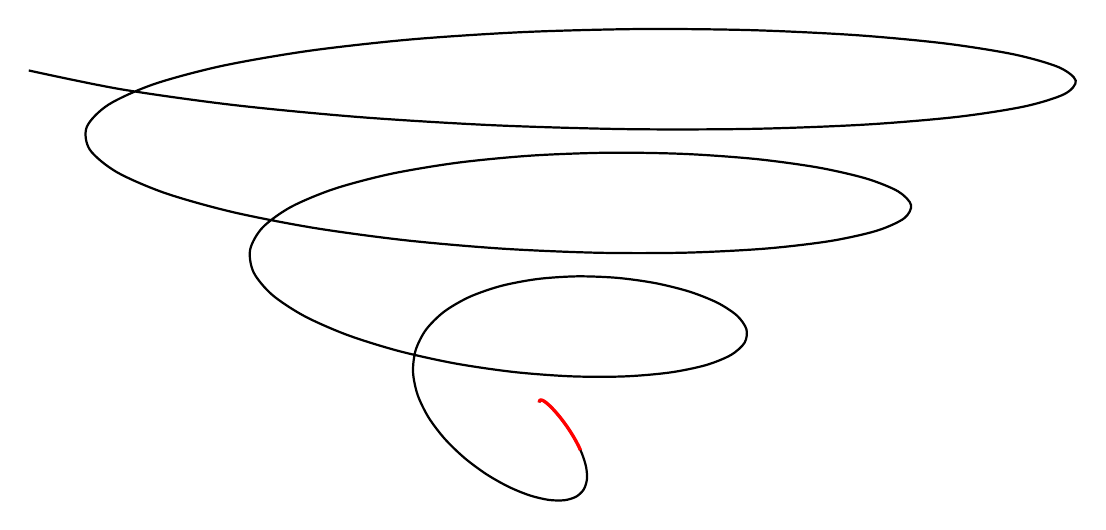
\begin{tikzpicture}
\draw[thick] plot[domain=0:23, smooth, samples=100]({sin( \x r)*\x/3},{cos(\x r)+\x/4});
\draw[very thick, red] plot[domain=0:1.57, smooth, samples=100]({sin( \x r)*\x/3},{cos(\x r)+\x/4});
\end{tikzpicture}
\end{center}
Due to the restricted domain, our actual curve is only one-quarter of a ``turn" of this spiral, indicated in red above.

The parameter $z$ is a measure of height, and it is also a radian measure as the spiral turns.
\end{solution}
%%%%%%%%%%%%%%%%%%


\begin{question}
Reparametrize the function $\vr(t)=(\tfrac12 t^2 , \tfrac13 t^3)$ in terms of arclength from $t=-1$.
\end{question}
\begin{hint}
Remember $\sqrt{x^2}=|x|$. You will need to consider cases for this one.
\end{hint}
\begin{answer}
$\vR(s)=\begin{cases}
\Big(\frac12\left[ (2\sqrt2-3s)^{2/3}-1\right],-\frac13\left[(2\sqrt2-3s)^{2/3}-1\right]^{3/2}\Big)&\text{ when }s\le \frac13(2\sqrt2-1)\\
\Big(\frac12\left[(3s+2-2\sqrt2)^{2/3}-1 \right],\frac13\left[(3s+2-2\sqrt2)^{2/3}-1\right]^{3/2}\Big)&\text{ when }s>\frac13(2\sqrt2-1)
\end{cases}
$
\end{answer}
\begin{solution}
\begin{align*}
\vr(t)&=(\tfrac12 t^2 , \tfrac13 t^3)\\
\vr'(t)&=(t,t^2)\\
|\vr'(t)|&=\sqrt{t^2+t^4}=|t|\sqrt{1+t^2}\\
s(t)&=\int_{-1}^t|x|\sqrt{1+x^2}\dee{x}=\begin{cases}
\int_{-1}^t -x\sqrt{1+x^2}\dee{x} & \text{when } t \le 0\\
\int_{-1}^0 -x\sqrt{1+x^2}\dee{x} +\int_{0}^t x\sqrt{1+x^2}\dee{x} & \text{when } t > 0\\
\end{cases}
\intertext{Let $u=1+x^2$, $\frac12\dee{u}=x\dee{x}$}
&=\begin{cases}
-\int_{2}^{1+t^2} \frac{1}{2}\sqrt{u}\dee{u} & \text{when } t \le 0\\
-\int_{2}^1 \frac12\sqrt{u}\dee{u}+ \int_{1}^{1+t^2} \frac12\sqrt{u}\dee{u} & \text{when } t > 0\\
\end{cases}
\\&=\begin{cases}
 -\frac{1}{3}u^{3/2}|_{2}^{1+t^2} & \text{when } t \le 0\\
-\frac{1}{3}u^{3/2}|_{2}^{1}+  \frac13u^{3/2}|_{1}^{1+t^2} & \text{when } t > 0\\
\end{cases}
\\&=\begin{cases}
 \frac{2^{3/2}}{3}-\frac{1}{3}(1+t^2)^{3/2} & \text{when } t \le 0\\
-\frac23+\frac{2^{3/2}}{3}+\frac13(1+t^2)^{3/2} & \text{when } t > 0\\
\end{cases}
\intertext{Solving for $t$ in terms of $s$:}
1+t^2&=\begin{cases}(2\sqrt2-3s)^{2/3} &\text{when } t \le 0\\
(3s+2-2\sqrt{2})^{2/3} &\text{when }t>0\end{cases}\\
t^2&=\begin{cases}(2\sqrt2-3s)^{2/3}-1 &\text{when } t \le 0\\
(3s+2-2\sqrt{2})^{2/3}-1 &\text{when }t>0
\end{cases}
\intertext{Remembering that $\sqrt{t^2}=|t|$:}
t&=\begin{cases}-\sqrt{(2\sqrt2-3s)^{2/3}-1} &\text{when } t \le 0\\
\sqrt{(3s+2-2\sqrt{2})^{2/3}-1} &\text{when }t>0
\end{cases}
\intertext{Noting that $t=0$ when $s=\tfrac{1}{3}(2\sqrt2-1)$, we find our reparametrization of $(\tfrac12t^2,\tfrac13t^3)$.}
\vR(s)&=\begin{cases}
\Big(\frac12\left[ (2\sqrt2-3s)^{2/3}-1\right],-\frac13\left[(2\sqrt2-3s)^{2/3}-1\right]^{3/2}\Big)&\text{ when }s\le \frac13(2\sqrt2-1)\\
\Big(\frac12\left[(3s+2-2\sqrt2)^{2/3}-1 \right],\frac13\left[(3s+2-2\sqrt2)^{2/3}-1\right]^{3/2}\Big)&\text{ when }s>\frac13(2\sqrt2-1)
\end{cases}
\end{align*}
Remark: after a computation with this much detail, it's nice to find a few points to check, to verify that our answer is reasonable. For instance, when $s=0$, $t$ should be $-1$, and vice-versa. Also, we found that $t=0$ corresponds to $s=\frac13(2\sqrt2-1)$. So, we should be able to verify that $\vr(0)=\vR\left(\frac13(2\sqrt2-1)\right)$ and $\vr(-1)=\vR(0)$.
\end{solution}
%%%%%%%%%%%%%%%%%%

%%%%%%%%%%%%%%%%%%

\section{Curvature}
%\documentclass[12pt]{article}

\questionheader{ex:s1.3}

%%%%%%%%%%%%%%%%%%
\subsection*{\Conceptual}
%%%%%%%%%%%%%%%%%%
%%%%%%%%%%%%%%%%%%%
\Instructions{There are a lot of constants in this chapter that might be new to you. They can take a little getting used to. Questions \ref{prob_s1.3:constantsa}-\ref{prob_s1.3:constantsb} provide practice working with and interpreting these constants and their relations to each other.}
\begin{question}\label{prob_s1.3:constantsa}
Sketch the curve $\vr(t)=(3\sin t,3\cos t)$. At the point $(0,3)$, label $\hT$ and $\hN$. Give the values of $\kappa$ and $\rho$ at this point as well.
\end{question}
\begin{hint}
The curve is a circle, so you don't need to do any calculus.
\end{hint}
\begin{answer} 
\begin{tikzpicture}
\YEaxis{2}{2}
\YExcoord{.5}{1}
\draw node[shape=circle, minimum size=3cm, draw]{};
\draw (0,1.5) node[vertex]{};
\draw[ultra thick, red, ->] (0,1.5)--(.5,1.5) node[right]{$\hT$};
\draw[ultra thick, blue, ->] (0,1.5)--(0,1) node[below left]{$\hN$};
\end{tikzpicture}
\\
$\rho=3$, $\ka=\frac13$
\end{answer}
\begin{solution}
The curve is a circle of radius 3, centred at the origin. So, the ``circle of best fit" is just the curve itself. $\hT$ is the unit vector tangent to the circle in direction of increasing $t$, and $\hN$ is the unit vector pointing towards the origin.
\begin{center}
\begin{tikzpicture}
\YEaxis{2}{2}
\YExcoord{.5}{1}
\draw node[shape=circle, minimum size=3cm, draw]{};
\draw (0,1.5) node[vertex]{};
\draw[ultra thick, red, ->] (0,1.5)--(.5,1.5) node[right]{$\hT$};
\draw[ultra thick, blue, ->] (0,1.5)--(0,1) node[below left]{$\hN$};
\end{tikzpicture}
\end{center}
The radius of the (osculating) circle is 3, so $\rho=3$ and $\ka=\frac1\rho=\frac13$.
\end{solution}
%%%%%%%%%%%%%%%%%%%
\begin{question}
Consider the circle $\vr(t)=(3\sin t,3\cos t)$. Find $\hT(t)$ and $\hT(s)$. Then, use parts (\eref{CLP317}{thm:curvatureFormulae:part:b}) and (\eref{CLP317}{thm:curvatureFormulae:part:c}) of Theorem~\eref{CLP317}{thm:curvatureFormulae} to find $\hN(t)$ and $\hN(s)$.
\end{question}
\begin{hint}
Because $\vr$ is a circle, you can parametrize it with respect to arclength without using an integral. You found $\ka$ in  Question~\ref{prob_s1.3:constantsa}.
\end{hint}
\begin{answer}
$\hT(t)=(\cos t, -\sin t) $, $\hT(s)=(\cos(s/3),-\sin(s/3))$,\\
$\hN(t)=(-\sin t ,-\cos t)$, $\hN(s)=\left(-\sin(s/3),-\cos(s/3) \right)$
\end{answer}
\begin{solution}
The arclength of $\vr(t)$ traced out by an interval of $t$ of length $\theta$ is $3\theta$. That is, $s=3t$. Our reparametrization of the circle in terms of arclength is $\vR(s)=(3\sin(s/3),3\cos(s/3))$.

We can calculate the vectors tangent to the circle, then normalize them (i.e. make them length one) to find $\hT$.
\begin{align*}
\vv(t)&=\vr'(t)=(3\cos t, -3\sin t) & \hT(s)&=\vR'(s)=(\cos(s/3),-\sin(s/3))\\
\hT(t)&=\frac{\vr'(t)}{|\vr'(t)|}=\frac{(3\cos t, -3\sin t)}{3}=(\cos t, -\sin t) 
\end{align*}
Note $\vR'(s)$, because it's parametrized in terms of arclength, has derivative vectors of length one. So, we don't need to normalize them (although if we did, it wouldn't change anything).

Note also that we can check out answers using Question~\ref{prob_s1.3:constantsa}. In that question, we found $\hT$ was $\hi$ when $t=s=0$; this fits with the vectors we just found.

As in Question~\ref{prob_s1.3:constantsa}, $\ka=\frac13$. So, using Theorem~\eref{CLP317}{thm:curvatureFormulae} Part (\eref{CLP317}{thm:curvatureFormulae:part:b}):
\begin{align*}
\diff{\hT}{s}(s) &= \ka(s)\,\hN(s)\\
\left(-\frac13\sin(s/3)~,~-\frac13\cos(s/3) \right)&=\frac13\hN(s)\\
\left(-\sin(s/3)~,~-\cos(s/3) \right)&=\hN(s)
\end{align*}

Remember $s=3t$. Using Theorem~\eref{CLP317}{thm:curvatureFormulae} Part (\eref{CLP317}{thm:curvatureFormulae:part:c}):
\begin{align*}
\diff{\hT}{t} &= \ka \diff{s}{t} \hN(t)\\
(-\sin t ,-\cos t) &= \frac13 (3) \hN(t)\\
(-\sin t ,-\cos t) &= \hN(t)
\end{align*}
\end{solution}
%%%%%%%%%%%%%%%%%%%
%%%%%%%%%%%%%%%%%%%
\begin{question}
The functon $\vr(t)=(t\cos t, t\sin t)$, $t \ge 0$, defines a spiral centred at the origin. 
Using only geometric intuition (no calculation), predict $\displaystyle\lim_{t \to \infty}\kappa(t)$.
\end{question}
\begin{hint}
When $t$ is large, does the spiral locally look like a circle of large radius, or small?
\end{hint}
\begin{answer}
$\lim\limits_{t \to \infty}\ka(t)=0$
\end{answer}
\begin{solution}
As $t$ increases, the arms of the spiral ``flatten out," looking like a circle of bigger and bigger radius. So, we would expect the curvature to decrease: $\lim\limits_{t \to \infty}\ka(t)=0$. 
\begin{center}
	
\includegraphics{fig/spiral2d.pdf}
\end{center}
\end{solution}
%%%%%%%%%%%%%%%%%%%
\begin{question}
Let $\vr(t)=(e^t,3t,\sin t)$. What is $\diff{s}{t}$?
\end{question}
\begin{hint}
$\diff{s}{t}=\left| \vv(t)\right|=\left| \vr'(t)\right|$
\end{hint}
\begin{answer}
$\diff{s}{t}=\sqrt{e^{2t}+9+\cos^2 t}$
\end{answer}
\begin{solution}
$\diff{s}{t}=\left| \vv(t)\right|=\left| \vr'(t)\right|=\left| (e^t,3,\cos t)\right|=\sqrt{e^{2t}+9+\cos^2 t}$
\end{solution}
%%%%%%%%%%%%%%%%%%%
\begin{question}\label{prob_s1.3:constantsb}
In Question~\ref{prob_s1.2:spiral} of Section~\eref{CLP317}{sec:reparam},%%%section 1.2
we found that the spiral \[\vr(t) = e^t (\cos t, \sin t)\] parametrized in terms of arclength is 
\[\vR(s)=\frac{s}{\sqrt{2}}\left(\cos\Big(\ln\Big(\frac{s}{\sqrt{2}}\Big)\Big)\,,\,
                 \sin\Big(\ln\Big(\frac{s}{\sqrt{2}}\Big)\Big)\right).\]
                 
Find $\diff{\hT}{s}$ and $\diff{\hT}{t}$ for this curve.
\end{question}
\begin{hint}
$\hT=\frac{\vv(t)}{|\vv(t)|}=\frac{\vr'(t)}{|\vr'(t)|}$
\end{hint}
\begin{answer}
$ \diff{\hT}{t}=\frac1{\sqrt2}\big(-\sin t - \cos t~,~-\sin t + \cos t\big)$\\
$\diff{\hT}{s}=\frac{1}{\sqrt{2}\,s}\left( -\sin \left(\ln\left( s/\sqrt{2}\right)\right)-\cos\left(\ln\left( s/\sqrt{2}\right)\right))~,~-\sin \left(\ln\left( s/\sqrt{2}\right)\right)+\cos \left(\ln\left( s/\sqrt{2}\right)\right)\right)$
\end{answer}
\begin{solution}
\begin{align*}
\hT(t)&=\frac{\vv(t)}{|\vv(t)|}=\frac{\vr'(t)}{|\vr'(t)|}
\intertext{We use the chain rule to differentiate $\vr(t)$.}
&=\frac{\big(e^t(\cos t - \sin t)~,~e^t(\cos t + \sin t)\big)}{\sqrt{e^{2t}(\cos t - \sin t)^2+e^{2t}(\cos t + \sin t)^2}}\\
&=\frac1{\sqrt2}\big(\cos t - \sin t~,~\cos t + \sin t\big)\\
\diff{\hT}{t}&=\frac1{\sqrt2}\big(-\sin t - \cos t~,~-\sin t + \cos t\big)
\intertext{Since $\vR(s)$ is parametrized with respect to arclength, $|\vR'(s)|=1$.}
\hT(s)&=\vR'(s)
\intertext{Making ample use of the chain rule, and setting $U(s)=\left(\ln\left( s/\sqrt{2}\right)\right)$, we have $U'(s)=\frac{1}{s}$:}
\hT(s)&=\frac{1}{\sqrt2}\left( \cos U(s)-\sin U(s)~,~ \cos U(s) + \sin U(s)\right)\\
\diff{\hT}{s}&=\frac{1}{\sqrt{2}\,s}\left( -\sin U(s)-\cos U(s)~,~-\sin U(s)+\cos U(s)\right)
\end{align*}
\end{solution}

%%%%%%%%%%%%%%%%%%%
\begin{question}
In this exercise, we make more precise the sense in which the osculating 
circle is the circle which best approximates a plane curve at a point.
\begin{itemize}\itemsep1pt \parskip0pt \parsep0pt %\itemindent-15pt
\item
By translating and rotating our coordinate system, we
can always arrange that the point is $(0,0)$ and that the curve is
$y=f(x)$ with $f'(0)=0$ and $f''(0)>0$. (We are assuming that
the curvature at the point is nonzero.) 
\item
Let $y=g(x)$ be the bottom half of the circle of radius $r$ which 
is centred at $(0,r)$. 
\end{itemize}
Show that if $f(x)$ and $g(x)$ have the 
same second order Taylor approximation at $x=0$, then $r$ is the 
radius of curvature of $y=f(x)$ at $x=0$.
\end{question}

%\begin{hint}
%\end{hint}

\begin{answer}
See the solution.
\end{answer}

\begin{solution}
The circle  of radius $r$ centred at $(0,r)$ is $x^2+(y-r)^2 = r^2$.
The bottom half of this circle is 
\begin{equation*}
y = g(x) = r - \sqrt{r^2-x^2}
\end{equation*}
So
\begin{alignat*}{3}
g'(x) &=\frac{x}{\sqrt{r^2-x^2}} &
g'(0) &=0 \\
g''(x)&=\frac{1}{\sqrt{r^2-x^2}} +\frac{x^2}{[{r^2-x^2]}^{3/2}}\qquad &
g''(0)&=\frac{1}{r}
\end{alignat*}
As $f(x)$ and $g(x)$ have the same second order Taylor approximation at $x=0$,
$f''(0) = g''(0) = \frac{1}{r}$. 

We may parametrize the curve by $\vr(x) = x\,\hi + f(x)\,\hj$.
So
\begin{alignat*}{3}
\vr'(x)& = \hi +f'(x)\,\hj\qquad &
\vr'(0)& = \hi +f'(0)\,\hj = \hi \\
\vr''(x)& = f''(x)\,\hj &
\vr''(0)& = f''(0)\,\hj \\[0.05in]
\ka(0)& = \frac{|\vr'(0)\times\vr''(0)|}{|\vr'(0)|^3}
 = \frac{|f''(0)\,\hi\times\hj|}{|\hi|^3}
=f''(0)\hidewidth
\end{alignat*}
So $\ka(0)=f''(0)=\frac{1}{r}$ and $r$ is indeed the radius of curvature
of $y=f(x)$ at $x=0$.
\end{solution}


%%%%%%%%%%%%%%%%%%
\subsection*{\Procedural}
%%%%%%%%%%%%%%%%%%
\begin{question}
Given a curve $\vr(t)=(e^t,t^2+t)$, compute the following quantities:
\begin{enumerate}[A.]
\item $\vv(t)$
\item $\va(t)$
\item $\diff{s}{t}$
\item $\hT(t)$
\item $\ka(t)$
\end{enumerate}
\end{question}
\begin{hint}
You can find the last two quantities by making use of the first three. Looking ahead, the formula list in Section~\eref{CLP317}{sec:CurveCompendium} might come in handy. 
\end{hint}
\begin{answer}
\begin{enumerate}[A.]
\item $\vv(t)=(e^t,2t+1)$
\item $\va(t)=(e^t,2)$
\item $\diff{s}{t}=\sqrt{e^{2t}+(2t+1)^2}$
\item $\displaystyle\hT(t)=\left(
 \frac{e^t}{\sqrt{e^{2t}+(2t+1)^2}},
 \frac{2t+1}{\sqrt{e^{2t}+(2t+1)^2}}
 \right)
$
\item $\displaystyle\ka(t)=\dfrac{e^t|1-2t|}{(e^{2t}+(2t+1)^2)^{3/2}}$
\end{enumerate}

\end{answer}
\begin{solution}
\begin{enumerate}[A.]
\item $\vv(t)=\vr'(t)=(e^t,2t+1)$
\item $\va(t)=\vr''(t)=(e^t,2)$
\item $\diff{s}{t}=|\vv(t)|=\sqrt{e^{2t}+(2t+1)^2}$
\item $\displaystyle\hT(t)=\frac{\vv(t)}{|\vv(t)|}=\frac{(e^t,2t+1)}{\sqrt{e^{2t}+(2t+1)^2}}=\left(
 \frac{e^t}{\sqrt{e^{2t}+(2t+1)^2}},
 \frac{2t+1}{\sqrt{e^{2t}+(2t+1)^2}}
 \right)
$
\item $\displaystyle\ka(t)=\frac{|\vv(t) \times \va(t)|}{\left(\diff{s}{t}\right)^3}=\frac{\left| (e^t,2t+1)\times(e^t,2)\right|}{\sqrt{e^{2t}+(2t+1)^2}^3}=\dfrac{e^t|1-2t|}{(e^{2t}+(2t+1)^2)^{3/2}}$
\end{enumerate}

\end{solution}
%%%%%%%%%%%%%%%%%%

%%%%%%%%%%%%%%%%%%%%%%%%%%%
\begin{question}
Find the curvature $\ka(t)$ of $\vr(t)=(\cos t+\sin t , \sin t - \cos t)$.
\end{question}
\begin{hint}
We can calculate $\ka = \dfrac{|\vv(t) \times \va(t)|}{\left| \left(\diff{s}{t}\right)^3\right|}$. We can also figure out what kind of a shape our curve is.
\end{hint}
\begin{answer}
$\ka(t)=\frac{1}{\sqrt{2}}$
\end{answer}
\begin{solution}
\begin{description}
\item[Solution 1:] Note that $(\cos t+\sin t )^2+(\sin t - \cos t)^2=2$ for all $t$. So, the points $(x,y)$ of our curve lie on $x^2+y^2=2$, which is a circle of radius $\sqrt{2}$. Indeed
\begin{align*}
x(t)&= \cos t+\sin t 
=\sqrt{2}\big[\cos t \cos\tfrac{\pi}{4} +\sin t \sin\tfrac{\pi}{4}\big]
\\
&=\sqrt{2}\cos\big(t-\tfrac{\pi}{4}\big)
\\
y(t)&= \sin t-\cos t 
=\sqrt{2}\big[\sin t \cos\tfrac{\pi}{4}-\cos t\sin \tfrac{\pi}{4}\big]
\\
&=\sqrt{2}\sin\big(t-\tfrac{\pi}{4}\big)
\end{align*}
So, $\vr(t)$ circumnavigates a circle of radius $\sqrt{2}$ and consequently has curvature $\ka=\frac{1}{\sqrt{2}}$.
\item[Solution 2:]
We use the formula $\ka = \dfrac{|\vv(t) \times \va(t)|}{\left| \left(\diff{s}{t}\right)^3\right|}$, remembering that $\vv(t)=\vr'(t)$, $\va(t)=\vr''(t)$, and $\diff{s}{t}=\left| \vr'(t)\right|$.
\begin{align*}
\vv(t)&=\vr'(t)=(-\sin t +\cos t, \cos t + \sin t)\\
\va(t)&=\vr''(t)=(-\cos t  -\sin t, -\sin t + \cos t)\\
\vv(t) \times \va(t)&=\big[(-\sin t + \cos t)^2+(\cos t + \sin t)^2\big]\hk=2\hk\\
\diff{s}{t}&=\left|\diff{\vv}{t} \right|=\sqrt{(-\sin t + \cos t)^2+(\cos t + \sin t )^2}=\sqrt2\\
\ka&=\left|\frac{\vv(t) \times \va(t)}{\left(\diff{s}{t}\right)^3}\right|=\left|\frac{2\hk}{\sqrt{2}^3}\right|=\frac{1}{\sqrt 2}
\end{align*}
\end{description}
\end{solution}

%%%%%%%%%%%%%%%%%%%%%%%%%%%
\begin{question}
 Find the minimum and maximum values for the curvature of
the ellipse $x(t)= a \cos t$, $y(t)=b\sin t$. Here $a>b>0$.
\end{question}

\begin{hint} 
The maximum and minimum values of $\ka(t)$ should be
obvious from your formula for $\ka(t)$.
\end{hint}

\begin{answer} 
$\ka_{\rm max}=\frac{a}{b^2}$, $\ka_{\rm min}=\frac{b}{a^2}$.
\end{answer}

\begin{solution} 
 For the given ellipse
\begin{align*}
\vr(t)&= a\cos t\ \hi +b\sin t\ \hj \\
\vv(t)&= -a\sin t\ \hi +b\cos t\ \hj \\
|\vv(t)|& = \sqrt{a^2\sin^2t+b^2\cos^2 t}\\
\va(t)&= -a\cos t\ \hi -b\sin t\ \hj \\
\vv(t)\times\va(t) &=\det\left[\begin{matrix} \hi & \hj & \hk \\
                                        -a\sin t & b\cos t & 0 \\
                                        -a\cos t & -b\sin t & 0 
                                    \end{matrix}\right]
= ab\,\hk\\
\ka(t)&=\frac{|\vv(t)\times\va(t)|}{|\vv(t)|^3}
=\frac{ab}{{[a^2\sin^2t+b^2\cos^2 t]}^{3/2}}
\end{align*}
Hence the maximum (minimum) curvature is achieved when the denominator
is a minimum (maximum) which is the case when $\sin t =0$ ($\cos t=0$).
So $\ka_{\rm max}=\frac{a}{b^2}$ and $\ka_{\rm min}=\frac{b}{a^2}$.
\end{solution}




%%%%%%%%%%%%%%%%%%%%%%%%%%%
\begin{question}[M317 2018A] %1
\begin{enumerate}[(a)]
\item 
Find the curvature of $y=e^x$ at $(0,1)$.
\item
Find the equation of the circle best fitting $y=e^x$
at $(0,1)$.
\end{enumerate}
\end{question}

%\begin{hint} 
%\end{hint}

\begin{answer} 
(a) $\ka(0)=2^{-3/2}$ \qquad
(b) $(x+2)^2+(y-3)^2=8$
\end{answer}

\begin{solution} 
Parametrize the curve by $\vr(t) = t\,\hi +e^t\,\hj$. Then
\begin{align*}
\vv(t) & = \hi + e^t\,\hj  &
\vv(0) & = \hi +\hj &
\frac{ds}{dt} &=|\vv(t)|=\sqrt{1+e^{2t}} &
\hT(t) & = \frac{\vv(t)}{|\vv(t)|} = \frac{\hi+e^t\hj}{\sqrt{1+e^{2t}}}\\
\va(t) & =  e^t\,\hj  &
\va(0) & = \hj \ &
\frac{ds}{dt}(0) &=\sqrt{2} &
\hT(0) & = \frac{\vv(0)}{|\vv(0)|} = \frac{\hi+\hj}{\sqrt{2}}
\end{align*}

(a) We're given $y$ in terms of $x$, so let's use
 Part (\eref{CLP317}{thm:curvatureFormulae:part:e}) of Theorem~\eref{CLP317}{thm:curvatureFormulae}:
 \begin{align*}
 \ka 
&=\frac{\big|\difftwo{y}{x}\big|}
{ {\big[1+\big(\diff{y}{x}\big)^2\big]}^{3/2} } = 
\frac{e^x}
{ {\big[1+\big(e^x\big)^2\big]}^{3/2} } \\
\ka(0)&=\frac{1}{[1+1]^{3/2}}=2^{-3/2}
 \end{align*}


%Since
%\begin{align*}
%\vv(0)\times\va(0) = \hk = \ka(0)\,\big(\frac{ds}{dt}(0)\big)^3\,\hat\vB
%=\ka(0)\,2^{3/2}\, \hat\vB
%\end{align*}
%we have $\ka(0)=2^{-3/2}$ and $\hat\vB=\hk$.
%%%these solutions used \vB, which appears in the NEXT chapter of the text; I've changed it to align more with section 1.3


(b)
\begin{itemize}
\item  The radius of the circle we want is $\rho=\frac{1}{\ka}=2^{3/2}$. If its centre is at $(a,b)$, then the circle will have equation $(x-a)^2+(y-b)^2=2^3$. So, we will find its centre.

\item The unit vector $\hN$ points from our point $(0,1)$ towards the centre of the circle. Since the radius of the circle is $2^{3/2}$, the centre of the circle will be at $(0,1)+2^{3/2}\hN$. So, we'll find $\hN$.

\item Since $\hN$ is a unit vector perpendicular to $\hT=\dfrac{\hi+\hj}{\sqrt 2}$, we know $\hN$ will be either $\dfrac{\hi-\hj}{\sqrt 2}$ or $\dfrac{-\hi+\hj}{\sqrt 2}$.

\item Using Part~(\eref{CLP317}{clpcurvesthm:curvatureFormulae:partd}) of the proof of Theorem~\eref{CLP317}{thm:curvatureFormulae}:
\begin{align*}
\vv(t) \times \va(t) &= \ka\left(\diff{s}{t}\right)^3\hT \times \hN\\
(\hi+\hj)\times(\hj)&=2^{-3/2}\left(\sqrt2 \right)^3\frac{\hi+\hj}{\sqrt 2}\times\hN\\
\hk &=\frac{1}{\sqrt2}(\hi + \hj)\times\hN\\
\hN&=\frac{-\hi+\hj}{\sqrt2}
 \end{align*}
So, the centre of our circle is at point $(0,1)+\rho\hN=(0,1)+2^{3/2}\frac{-\hi+\hj}{2^{1/2}}=(-2,3)$. Then the equation of the circle is $(x+2)^2+(y-3)^2=8$.
\end{itemize}
%We have
%\begin{equation*}
%\hN(0) = \hat\vB(0)\times\hT(0) = \frac{1}{\sqrt{2}}\hk\times(\hi+\hj)
%=\frac{1}{\sqrt{2}}(-\hi+\hj)
%\end{equation*}
%so that the radius of curvature is $\frac{1}{\ka(0)}=2^{3/2}$ and 
%centre of curvature is
%\begin{align*}
%(0,1) + \frac{1}{\ka(0)}\hN(0) = (0,1) +2^{3/2} 2^{-1/2}(-1,1)=(-2,3)
%\end{align*}
%and the equation of the osculating circle is 
%$(x+2)^2+(y-3)^2=8$. 
\end{solution}


%%%%%%%%%%%%%%%%%%%%%%%%%%%%%%%
\begin{question}[M317 2011A] %1
\item   %1
Consider the motion of a thumbtack stuck in the tread of a tire which 
is on a bicycle moving at constant speed. This motion is given by 
the parametrized curve 
\begin{equation*}
\vr(t) = \big(t - \sin t\,,\, 1 - \cos t\big)
\end{equation*}
with $t > 0$.
\begin{enumerate}[(a)]
\item
Sketch the curve in the $xy$-plane for $0 < t < 4\pi$.
\item
Find and simplify the formula for the curvature $\kappa(t)$.
\item
Find the radius of curvature of the osculating circle to 
$\vr(t)$ at $t = \pi$.
\item
Find the equation of the osculating circle to $\vr(t)$ at $t = \pi$.
\end{enumerate}
\end{question}

\begin{hint} 
For part (a), determine $\vr(0)$, $\vr(\pi)$, $\vr(2\pi)$, $\vr(3\pi)$, and $\vr(4\pi)$, to help you map out the motion. Also visualize the thumbtack as the wheel moves.

For part (d), use the fact that you only care about $t=\pi$: where is this on your sketch? What does that mean about the direction of $\hN$?
\end{hint}

\begin{answer} 
(a)
\begin{center}
    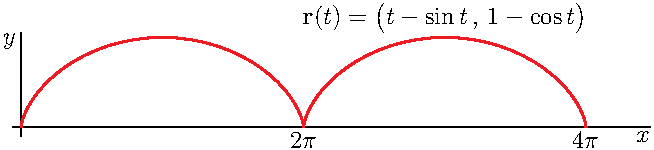
\includegraphics{fig/tack.pdf}
\end{center}

(b) $\ka(t) = \frac{1}{2^{3/2}\sqrt{1-\cos t}}$\qquad
(c) $4$\qquad
(d) $(x-\pi)^2 +(y+2)^2 = 16$
\end{answer}

\begin{solution} (a)
Think of 
\begin{equation*}
\vr(t) = (t,1) - (\sin t,\cos t)
\end{equation*}
The $(t,1)$ part gives the position of the centre of the wheel at time
$t$. The other part gives the position of the thumbtack with respect to
the centre of the wheel. In particular,
\begin{itemize}\itemsep1pt \parskip0pt \parsep0pt %\itemindent-15pt
\item[$\circ$]
at time $t=0$, $\vr(0) = (0,0)$. The thumbtack is on the ground (i.e. at $y=0$).
\item[$\circ$]
At time $t=\pi$, $\vr(\pi) = (\pi,2)$. The thumbtack is at its highest point (i.e. at $y=2$) and is above the centre of the wheel at $x=\pi$.
\item[$\circ$]
At time $t=2\pi$, $\vr(2\pi) = (2\pi,0)$. The thumbtack is back on the ground (i.e. at $y=0$) and is below the centre of the wheel at $x=2\pi$.
\item[$\circ$]
At time $t=3\pi$, $\vr(3\pi) = (3\pi,2)$. The thumbtack is again at its highest point (i.e. at $y=2$) and is above the centre of the wheel at $x=3\pi$.
\item[$\circ$]
At time $t=4\pi$, $\vr(4\pi) = (4\pi,0)$. The thumbtack is back on the ground (i.e. at $y=0$) and is below the centre of the wheel at $x=4\pi$.
\end{itemize}
Here is a sketch of the curve.
\begin{center}
    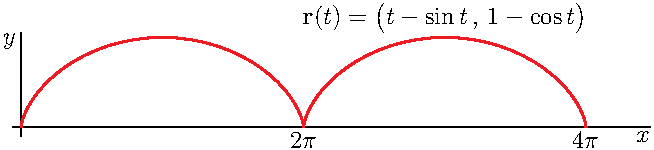
\includegraphics{fig/tack.pdf}
\end{center}

(b) Since 
\begin{align*}
\vr(t) &= \big(t - \sin t\,,\, 1 - \cos t\big) \\
\vv(t) =\vr'(t)&= \big(1-\cos t\,,\, \sin t\big) \\
\diff{s}{t}(t)=|\vv(t)|&=\sqrt{2-2\cos t} \\
\va(t) = \vv'(t)&=\big(\sin t\,,\, \cos t\big)  \displaybreak[0]\\
\vv(t)\times \va(t)&=\det\left[\begin{matrix}\hi&\hj&\hk\\[0.03in] 
     1-\cos t & \sin t & 0 \\
     \sin t  & \cos t & 0\end{matrix}\right]
=\big(\cos t-1\big)\,\hk
\end{align*}
the curvature
\begin{align*}
\ka(t) =\frac{|\vv(t)\times\va(t)|}{|\vv(t)|^3}
       =\frac{|\cos t-1|}{(2-2\cos t)^{3/2}}
       =\frac{1}{2^{3/2}\sqrt{1-\cos t}}
\end{align*}

(c) The radius of curvature at time $t=\pi$ is
\begin{equation*}
\rho(\pi) = \frac{1}{\ka(\pi)}
          = \frac{1}{1/2^{3/2}\sqrt{2}}
          =4
\end{equation*}

(d) At time $\pi$, the tack is at $\vr(\pi)=(\pi,2)$, which is at the top 
of its trajectory. Looking at the sketch in part (a), we see that,
at that time $\hN(\pi) = -\hj$.
So the osculating circle at time $t=\pi$ has center
\begin{equation*}
\vr(\pi) + \rho(\pi) \hN(\pi)
=(\pi,2) + 4(0,-1)
=(\pi,-2)
\end{equation*}
and radius $\rho(\pi)=4$. So the equation  of the osculating circle
at time $\pi$ is
\begin{equation*}
(x-\pi)^2 +(y+2)^2 = 16
\end{equation*}
\end{solution}





%%%%%%%%%%%%%%%%%%
\subsection*{\Application}
%%%%%%%%%%%%%%%%%%

%%%%%%%%%%%%%%%%%%%%%%%%%%%
\begin{question}
 Find the curvature $\ka$ as a function of arclength $s$ 
(measured from $(0,0)$) for the curve
\begin{equation*}
x(\theta)=\int_0^\theta \cos\big(\half\pi t^2\big)dt\quad \quad
y(\theta)=\int_0^\theta \sin\big(\half\pi t^2\big)dt
\end{equation*}
\end{question}

\begin{hint} 
You should find that $s=\theta$!
\end{hint}

\begin{answer} 
$\ka(s)=\pi s$
\end{answer}

\begin{solution} 
The velocity vector is
\begin{equation*}
\vv(\theta)=x'(\theta)\,\hi+y'(\theta)\,\hj
= \cos\big(\half\pi\theta^2\big)\,\hi + \sin\big(\half\pi\theta^2\big)\,\hj
\end{equation*}
Consequently the speed
\begin{equation*}
\diff{s}{\theta}(\theta)= |\vv(\theta)|=1
\implies s(\theta)=\theta+s(0)
\end{equation*}
Since $s(\theta)$ is zero when $\theta=0$, we have $s(\theta)=\theta$ and hence
\begin{equation*}
\hT(s)=\vv(s)
= \cos\big(\half\pi s^2\big)\,\hi + \sin\big(\half\pi s^2\big)\,\hj
\end{equation*}
so that
\begin{equation*}
\ka(s)=\left|\diff{\hT}{s}(s)\right|
=\big|-\pi s\sin\big(\half\pi s^2\big)\,\hi
+\pi s \cos\big(\half\pi s^2\big)\,\hj\big|
=\pi s
\end{equation*}
\end{solution}


%%%%%%%%%%%%%%%%%%%%%%%%%%%
\begin{question}[M317 2011D]  %3
Let $C$ be the curve in $\bbbr^2$ given by the graph of the function
$y=\frac{x^3}{3}$. Let $\kappa(x)$ be the curvature of $C$ at the point 
$(x, x^3/3)$. Find all points where $\ka(x)$ attains its maximal values,
or else explain why such points do not exist. What are the limits of 
$\kappa(x)$ as $x \rightarrow \infty$ and
$x \rightarrow -\infty$?
\end{question}

\begin{hint} 
Since $\ka(x)$ is never negative, $\ka(x)$ is maximum when $\ka^2(x)$ is maximum. The latter is easier to compute.
\end{hint}

\begin{answer} 
The maximum values occur at $(x,y)=\pm \big(1/\root{4}\of{5}\,,\,
                 \frac{1}{3}5^{-3/4}\big)$.

The limits $\lim_{x\rightarrow\pm\infty}\ka(x) = 0$.
\end{answer}

\begin{solution} 
The curve is $y=y(x)=\nicefrac{x^3}{3}$. Since $y'(x) = x^2$ and
$y''(x) = 2x$, the curvature is
\begin{align*}
\ka(x)
&=\frac{\big|\difftwo{y}{x}(x)\big|}
  {\Big[1+\big(\diff{y}{x}(x)\big)^2\Big]^{3/2}}
=\frac{\big|2x\big|}
  {\big[1+x^4\big]^{3/2}}
\end{align*}
 We'd like to find the critical points of $\ka(x)$, but differentiating it looks messy. Since $\ka(x)$ has only nonnegative values, its maxima correspond the the maxima of the function $\ka^2(x)$. So, we find the critical points of $\ka^2(x)$ instead, to save ourselves some computational toil.
\begin{align*}
0&=\diff{\hfill}{x}\ka(x)^2
=\diff{\hfill}{x}\frac{4x^2}{{(1+x^4)}^3}
=\frac{8x}{{(1+x^4)}^3} - 3\frac{16x^5}{{(1+x^4)}^4}
=\frac{8x(1+x^4)-3\times 16x^5}{{(1+x^4)}^4} \\
&=\frac{8x(1-5x^4)}{{(1+x^4)}^4}
\end{align*}
Note that $\ka(0)=0$ and $\ka(x)\rightarrow 0$ as $x\rightarrow\pm \infty$.
So the maximum occurs when $x=\pm 1/\root{4}\of{5}$.
\end{solution}

%\begin{question}[M317 2008D] %2
%Find the point in the first quadrant where the graph of the function 
%$y = \frac{1}{3} x^3$ has maximal curvature.
%\end{question}

%\begin{hint} 
%Find a formula for $\kappa(x)$, then maximize it using methods from first-semester calculus.
%\end{hint}

%\begin{answer} 
%$\big(\frac{1}{5^{1/4}}\,,\,\frac{1}{3\cdot 5^{3/4}}\big)$
%\end{answer}

%\begin{solution} 
%The specified curve is the graph of $y=f(x)$ with $f(x)=\frac{1}{3}x^3$.
%So, from \S \eref{CLP317}{sec:CurveCompendium} in the CLP-4 text, 
%the curvature is
%\begin{align*}
%\kappa(x) =\frac{|f''(x)|}{[{1+f'(x)^2]}^{3/2}}
%          =\frac{2|x|}{{[1+x^4]}^{3/2}}
%\end{align*}
%We are interested only in $x\ge 0$, so
%\begin{align*}
%\kappa(x) =\frac{2x}{{[1+x^4]}^{3/2}}
%\end{align*}
%As
%\begin{align*}
%\ka'(x) &= \frac{2}{{[1+x^4]}^{3/2}} 
%             -\frac{3}{2}\frac{2x(4x^3)}{{[1+x^4]}^{5/2}}
%=\frac{2-10x^4}{{[1+x^4]}^{5/2}}
%\end{align*}
%vanishes when $x=1/\root{4}\of{5}$, the only critical point of $\ka(x)$ occurs there. 

%We might want to satisfy ourselves that $x=1/\root{4}\of{5}$
%is a point of \emph{maximum} curvature (as opposed to, say, a point of minimum curvature). A sketch of $y=\frac{1}{3}x^3$ suggests this is the case, but we can also use the second derivative test:
%$
%\ka''(x)=\dfrac{60x^3(-1+x^4)}{(1+x^4)^{7/3}}$, so $\ka''(1/\root{4}\of{5})<0$, and our critical point is indeed the location of the maximum curvature.

%So, the curvature is maximum at the point
%$x=\frac{1}{5^{1/4}}$, $y=\frac{1}{3\cdot 5^{3/4}}$.


%\end{solution}



\section{Curves in Three Dimensions}
%\documentclass[12pt]{article}

\questionheader{ex:s1.4}

%%%%%%%%%%%%%%%%%%
\subsection*{\Conceptual}
%%%%%%%%%%%%%%%%%%
%%%%%%%%%%%%%%%%%%%
\begin{question}
In the sketch below of a three-dimensional curve and its osculating circle at a point, label $\hT$ and $\hN$. Will $\hB$ be pointing out of the paper towards the reader, or into the paper away from the reader?
\begin{center}
\begin{tikzpicture}%[scale=2]
\draw[thick] plot[domain=0:5]({sin(\x r)},\x);
\draw(.707,2.36) node[vertex]{};
\draw[ultra thick, ->, red] (.71,2.36)--(.14,3.18);
\draw[ultra thick, ->, red] (.71,2.36)--(-.11,1.78);
\draw[dashed] (-1.414,.86) node[shape=circle, draw, minimum size=5.2cm]{};
\end{tikzpicture}
\end{center}
\end{question}
\begin{hint}
	Use the right-hand rule to figure out how $\hB$ is oriented.
\end{hint}
\begin{answer}
\begin{center}
	\begin{tikzpicture}%[scale=2]
	\draw[thick] plot[domain=0:5]({sin(\x r)},\x);
	\draw(.707,2.36) node[vertex]{};
	\draw[ultra thick, ->, red] (.71,2.36)--(.14,3.18) node[above right]{$\hT$};
	\draw[ultra thick, ->, red] (.71,2.36)--(-.11,1.78)node[below left]{$\hN$};
	\draw[dashed] (-1.414,.86) node[shape=circle, draw, minimum size=5.2cm]{};
	\end{tikzpicture}
\end{center}
$\hB$ points out of the page (towards the reader).	
\end{answer}
\begin{solution}
	$\hT$ is tangent to the curve, while $\hN$ is perpendicular to it.
	\begin{center}
		\begin{tikzpicture}%[scale=2]
		\draw[thick] plot[domain=0:5]({sin(\x r)},\x);
		\draw(.707,2.36) node[vertex]{};
		\draw[ultra thick, ->, red] (.71,2.36)--(.14,3.18) node[above right]{$\hT$};
		\draw[ultra thick, ->, red] (.71,2.36)--(-.11,1.78)node[below left]{$\hN$};
		\draw[dashed] (-1.414,.86) node[shape=circle, draw, minimum size=5.2cm]{};
		\end{tikzpicture}
	\end{center}
Using the right-hand rule and $\hB=\hT \times \hN$, 	$\hB$ points out of the page (towards the reader).

To see this, point the fingers of your right hand in the direction of $\hT$, and curl them inwards until they are in the direction of $\hN$. To do this, your thumb must be pointing towards you, not away from you. Your thumb shows the direction of $\hT \times \hN$.
\end{solution}
%%%%%%%%%%%%%%%%%%%
%%%%%%%%%%%%%%%%%%%
\begin{question}
	In the formula
	\[\diff{s}{t}(t)=|\vv(t)|=|\vr'(t)|\]
	does $s$ stand for speed, or for arclength?
\end{question}
\begin{hint}
	Speed is the norm of velocity. Does that fit this equation?
\end{hint}
\begin{answer}
	arclength
\end{answer}
\begin{solution}
	In this equation, $s$ stands for arclength. 
	
	When we take a very small interval from $t$ to $t+h$, the change in arclength $s(t+h)-s(t)$ is approximately $|\vr(t+h)-\vr(t)|$, because our curve is approximated by a straight line. So, $\frac{s(t+h)-s(t)}{h} \approx \frac{|\vr(t+h)-\vr(t)|}{h}$, leading to $\diff{s}{t}=|\diff{\vr}{t}|=|\vv(t)|$.
	
The magnitude of velocity is speed; in this text we generally call this $v$. That is, $v=|\vv(t)|$. This leads to the potentially confusing (but standard) convention that $s$ stands for arclength, while $v$ stands for speed.
\end{solution}
%%%%%%%%%%%%%%%%%%%

%%%%%%%%%%%%%%%%%%%
\begin{question}
	Which curve (or curves) below have positive torsion, which have negative torsion, and which have zero torsion?
	 The arrows indicate the direction of increasing $t$.
\begin{center}	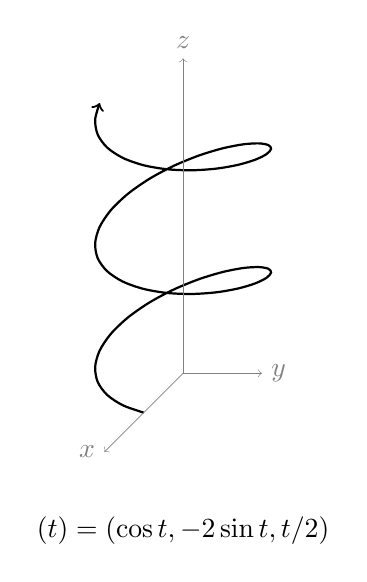
\begin{tikzpicture}
\draw[thick, ->] plot[domain=0:14, smooth, scale=0.5, samples=50]({-2*sin(\x r)-cos(\x r)},{\x/2-cos(\x r)});
\draw (0,-2) node{$\va(t)=(\cos t, -2\sin t, t/2)$};
\draw[help lines, ->] (0,0)--(0,4) node[above]{$z$};
\draw[help lines, ->] (0,0)--(-1,-1) node[left]{$x$};
\draw[help lines, ->] (0,0)--(1,0) node[right]{$y$};
	\end{tikzpicture}
\quad	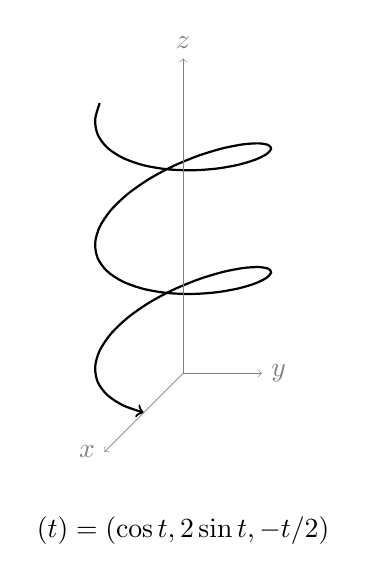
\begin{tikzpicture}
\draw[thick, ->] plot[domain=-14:0, smooth, scale=0.5, samples=50]({-2*sin(-\x r)-cos(\x r)},{-\x/2-cos(\x r)});
\draw (0,-2) node{$\vb(t)=(\cos t, 2\sin t, -t/2)$};
\draw[help lines, ->] (0,0)--(0,4) node[above]{$z$};
\draw[help lines, ->] (0,0)--(-1,-1) node[left]{$x$};
\draw[help lines, ->] (0,0)--(1,0) node[right]{$y$};
\end{tikzpicture}\quad	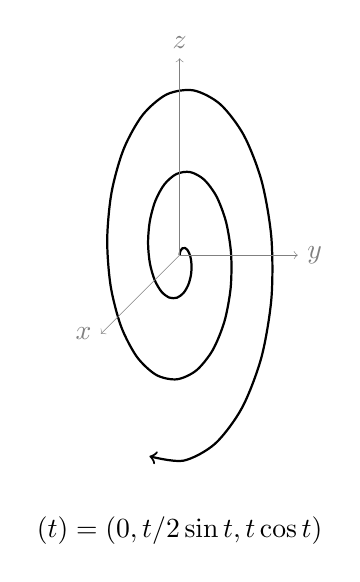
\begin{tikzpicture}
\draw[thick, ->] plot[domain=0:16, smooth, scale=0.5, samples=50]({\x*sin(\x r)/6},{\x/3*cos(\x r)});
\draw (0,-3.5) node{$\vc(t)=(0, t/2\sin t, t\cos t)$};
\draw[help lines, ->] (0,0)--(0,2.5) node[above]{$z$};
\draw[help lines, ->] (0,0)--(-1,-1) node[left]{$x$};
\draw[help lines, ->] (0,0)--(1.5,0) node[right]{$y$};
\end{tikzpicture}
\end{center}
\end{question}
\begin{hint}
Review Example~\eref{CLP317}{eg:helixTwist} %1.4.4
 and remember that positive torsion indicates ``right-handed twisting." You shouldn't actually need to calculate anything.
\end{hint}
\begin{answer}
	$\va(t)$ and $\vb(t)$ have negative torsion,  $\vc(t)$ has zero torsion.
\end{answer}
\begin{solution}
\textbf{Solution 1:}\\
	Curves $\va$ and $\vb$ are the same curve, just parametrized differently (replace $t$ with $-t$ to convince yourself if the picture isn't enough). So, they ought to have the same torsion.
	
	As in  Example~\eref{CLP317}{eg:helixTwist}, we imagine that the curve is the thread on a bolt. Take a look at your right hand. If your thumb is pointing up (corresponding to the $+z$ direction), and you're looking at the tip of your thumb, your fingers curl anticlockwise. Imagine a screw has threads matching the curves $\va$ and $\vb$, and we turn it anticlockwise. The screw would move down --- \emph{not} in the same direction as our thumb. So these curves are not right-handed helices, so they have negative torsion.
	
	The curve $\vc$ sits entirely in a plane (the plane $x=0$) so its torsion is zero everywhere.
	
\textbf{Solution 2:}\\
Here
is the conventional computation for both $\va(t)$ and $\vb(t)$.
(The upper sign is for $\va$ and the lower sign is for $\vb$.)
\begin{align*}
\vr(t)&=\big(\cos t\,,\,\mp 2\sin t \,,\,\pm t/2\big) \\
\vv(t)&=\big(-\sin t\,,\,\mp 2\cos t \,,\,\pm 1/2\big) \\
\va(t)&=\big(-\cos t\,,\,\pm 2\sin t \,,\,0\big) \\
\vv(t)\times\va(t)&=\big(-\sin t\,,\,\mp\cos t/2\,,\,\mp 2\big) \\
\diff{\va}{t}(t)&=\big(\sin t\,,\,\pm 2\cos t\,,\,0\big) \\
\vv(t)\times\va(t)\cdot \diff{\va}{t}(t) &= -1 \\
\tau(t)=\frac{\vv(t)\times\va(t)\cdot \diff{\va}{t}(t)}{|\vv(t)\times\va(t)|^2}
  &=-\frac{1}{\sin^2 t+\frac{1}{4}\cos^2 t+4}
   <0
\end{align*}
\end{solution}
%%%%%%%%%%%%%%%%%%%

%%%%%%%%%%%%%%%%%%%%%%%%%%%
\begin{question}
Consider a curve that is parametrized by arc length $s$.
\begin{enumerate}[(a)]
\item
Show that if the curve has curvature $\ka(s)=0$
for all $s$, then the curve is a straight line.

\item
Show that if the curve has curvature $\ka(s)>0$ and
torsion $\tau(s)=0$ for all $s$, then the curve lies in a plane.

\item
Show that if the curve has curvature $\ka(s)=\ka_0$,
a strictly positive constant, and torsion $\tau(s)=0$
for all $s$, then the curve is a circle.
\end{enumerate}
\end{question}

\begin{hint} 
(a) Show that the tangent vector $\hT(s)$ is a constant.

(b) Guess the plane. To do so, first show that the binormal $\hB(s)$ 
    is a constant. Then show that $(\vr(s)-\vr(0))\cdot\hB $ is a constant.

(c) Guess the circle. To do so, first show that $\vr_c(s)=\vr(s)+\frac{1}{\ka(s)}\hN(s)$ is a constant.

\end{hint}

\begin{answer} 

\end{answer}


\begin{solution}
(a) 
If $\ka(s)\equiv 0$, then 
$\diff{\hT}{s}=\ka(s)\hN(s)\equiv 0$ so that $\hT$ is a constant.
As a result $\diff{\vr}{s}(s)=\hT$ and $\vr(s) =s\hT+\vr(0)$ so that
the curve is the straight line with direction vector $\hT$ that passes
through $\vr(0)$.

(b) If $\tau(s)\equiv 0$, then 
$\diff{\hB}{s}=-\tau(s)\hN(s)\equiv 0$ so that $\hB$ is a constant.
As $\hT(s)\perp\hB$, 
\begin{equation*}
\diff{}{s} (\vr(s)-\vr(0))\cdot\hB =\hT(s)\cdot\hB=0
\end{equation*}
and $ (\vr(s)-\vr(0))\cdot\hB$ must be a constant. The constant
must be zero (set $s=0$), so $ (\vr(s)-\vr(0))\cdot\hB=0$ and $\vr(s)$
always lies in the plane through $\vr(0)$ with normal vector $\hB$.

(c) Parametrize the curve by arc length. Define the ``centre of 
curvature'' at $s$ by
\begin{equation*}
\vr_c(s)=\vr(s)+\frac{1}{\ka(s)}\hN(s)
\end{equation*}
Since $\ka(s)=\ka_0$ is a constant and $\tau(s)\equiv 0$,
\begin{equation*}
\diff{}{s}\vr_c(s)
   =\hT(s)+\frac{1}{\ka_0}\big[\tau(s)\hB-\ka(s)\hT\big]
   =\hT(s)+\frac{1}{\ka_0}\big[0\hB-\ka_0\hT\big]
   =0
\end{equation*}
Thus $\vr_c(s)=\vr_c$ is a constant and 
$\big|\vr(s)-\vr_c\big|=\frac{1}{\ka_0}$ lies on the sphere of radius
$\frac{1}{\ka_0}$ centred on $\vr_c$. Since $\tau(s)\equiv 0$,
the curve also lies on a plane, so it is a circle.
\end{solution}

%%%%%%%%%%%%%%%%%%%%%%%%%%%
\begin{question}[M317 2018A] %2
The surface $z=x^2+y^2$ is sliced by the plane $x=y$.
The resulting curve is oriented from $(0,0,0)$ to $(1,1,2)$.
\begin{enumerate}[(a)]
\item
Sketch the curve from $(0,0,0)$ to $(1,1,2)$.
\item
Sketch $\hat\vT$, $\hat\vN$ and $\hat\vB$ at $\big(\half,\half,\half\big)$.
\item
Find the torsion at $\big(\half,\half,\half\big)$.
\end{enumerate}
\end{question}

\begin{hint} 
It is not necessary to compute anything.
\end{hint}

\begin{answer} 
(a), (b)

\begin{center}
       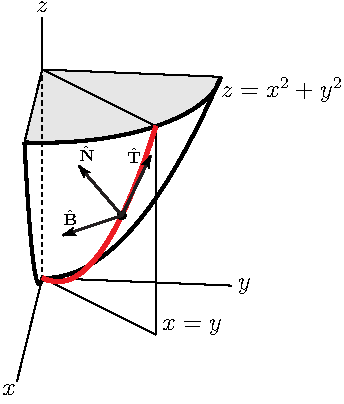
\includegraphics{parabolicBowlB.pdf}
\end{center}

(c) 
The torsion is zero.
\end{answer}

\begin{solution} 
(a), (b): $\hT$ points in the direction of the curve; $\hN$ is perpendicular to it, in the same plane, pointing towards the centre of curvature. Using the right-hand rule in the picture, we see $\hB$ is pointing to the left.

\begin{center}
       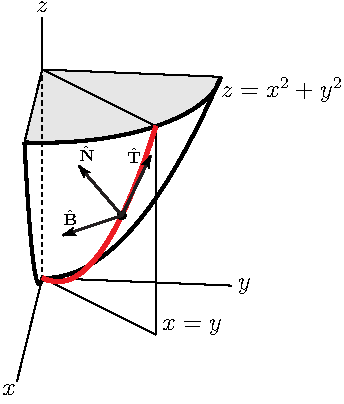
\includegraphics{parabolicBowlB.pdf}
\end{center}

(c) 
The torsion is zero, since the curve lies in a plane (the plane $x=y$).
\end{solution}



%%%%%%%%%%%%%%%%%%
\subsection*{\Procedural}
%%%%%%%%%%%%%%%%%%

%%%%%%%%%%%%%%%%%%%%%%%%%%%
\begin{question}[M317 2006A] %2
Let $C$ be the space curve
\begin{align*}
\vr(t) = \big(e^t - e^{-t}\big)\,\hi + \big(e^t + e^{-t}\big)\,\hj +2t\,\hk
\end{align*}
\begin{enumerate}[(a)]
\item
Find $\vr'$, $\vr''$ and the curvature of $C$.
\item
Find the length of the curve between $\vr(0)$ and $\vr(1)$.
\end{enumerate}
\end{question}

\begin{hint} 
Both parts of this question make use of the quantity $\diff{s}{t}$.
\end{hint}

\begin{answer} 
(a) $\vr'(t)=\big(e^t + e^{-t}\big)\,\hi + \big(e^t - e^{-t}\big)\,\hj +2\,\hk$,
    $\vr''(t)=\big(e^t - e^{-t}\big)\,\hi + \big(e^t + e^{-t}\big)\,\hj$,

\hskip0.75in    $\ka(t) =\frac{1}{2+e^{2t}+e^{-2t}}$

(b) $\sqrt{2}\Big[e-\frac{1}{e}\Big]$
\end{answer}

\begin{solution} (a)
As
\begin{align*}
\vr'(t)&=\big(e^t + e^{-t}\big)\,\hi + \big(e^t - e^{-t}\big)\,\hj +2\,\hk &
\diff{s}{t}(t) &=|\vr'(t)|= \sqrt{4+2e^{2t}+2e^{-2t}}
                =\sqrt{2}\big(e^t+e^{-t}\big)\\
\vr''(t)&=\big(e^t - e^{-t}\big)\,\hi + \big(e^t + e^{-t}\big)\,\hj   &
\vr'(t)\times\vr''(t)&=-2\big(e^t + e^{-t}\big)\,\hi 
          + 2\big(e^t - e^{-t}\big)\,\hj +4\,\hk
\end{align*}
the curvature
\begin{align*}
\ka(t) &= \frac{|\vv(t)\times\va(t)|}{\big(\diff{s}{t}\big)^3}
 =\frac{2\sqrt{4+2e^{2t}+2e^{-2t}}}{[4+2e^{2t}+2e^{-2t}]^{3/2}}
 =\frac{1}{2+e^{2t}+e^{-2t}}
\end{align*}

(b) The length of $C$ between $\vr(0)$ and $\vr(1)$ is
\begin{align*}
\int_0^1 \diff{s}{t}(t) \ \dee{t}
&= \sqrt{2} \int_0^1 (e^t+e^{-t}) \ \dee{t}
=\sqrt{2}\Big[e^t-e^{-t}\Big]_0^1
=\sqrt{2}\Big[e-\frac{1}{e}\Big]
\end{align*}


\end{solution}
%%%%%%%%%%%%%%%%%%%
\begin{question}
	Find the torsion of $\vr(t)=(t,t^2,t^3)$ at the point $(2,4,8)$.
\end{question}
\begin{hint}
	$\tau(t)=\dfrac{(\vv(t) \times \va(t))\cdot\diff{\va}{t}}{|\vv(t) \times \va(t)|^2}$
\end{hint}
\begin{answer}
$\frac{3}{{181}}$
\end{answer}
\begin{solution}
 The point $(2,4,8)$ occurs when $t=2$.
	\begin{align*}
		\vv(t)&=(1,2t,3t^2) & \vv(2)&=(1,4,12)\\
		\va(t)&=(0,2,6t) & \va(2)&=(0,2,12)\\
		\diff{\va}{t}(t)&=(0,0,6) & \diff{\va}{t}(2)&=(0,0,6)\\
		&& \vv(2) \times \va(2)&=(24,-12,2)\\
		&& |\vv(2) \times \va(2)|&=2\sqrt{181}
		\end{align*}
Now, we use a formula for torsion:
\begin{align*}\tau(t)&=\dfrac{(\vv(t) \times \va(t))\cdot\diff{\va}{t}(t)}{|\vv(t) \times \va(t)|^2}\\
\tau(2)&=\frac{(24,-12,2)\cdot(0,0,6)}{(2\sqrt{181})^2}=\frac{3}{{181}}
		\end{align*}
	
\end{solution}

%%%%%%%%%%%%%%%%%%%%%%%%%%%
\begin{question}
Find the unit tangent, unit normal and binormal vectors and
the curvature and torsion of the curve
\begin{equation*}
\vr(t)=t\,\hi + \frac{t^2}{2}\,\hj + \frac{t^3}{3}\,\hk
\end{equation*}
\end{question}

\begin{hint} 
Review \S\eref{CLP317}{sec:CurveCompendium} of the CLP-4 text.
\end{hint}

\begin{answer} 
$\hT(t)=\frac{\hi + t\,\hj + t^2\,\hk}{\sqrt{1+t^2+t^4}}$\qquad
$\hB(t)=\frac{t^2\,\hi-2t\,\hj+\hk}{\sqrt{1+4t^2+t^4}}$\qquad
$\hN(t)=\frac{-(t+2t^3)\,\hi+(1-t^4)\,\hj+(2t+t^3)\hk}
            {\sqrt{1+t^2+t^4}\sqrt{1+4t^2+t^4}}$

$\ka(t)=\frac{\sqrt{1+4t^2+t^4}}{[1+t^2+t^4]^{3/2}}$\qquad
$\tau(t)=\frac{2}{1+4t^2+t^4}$
\end{answer}


\begin{solution}
For the specified curve
\begin{align*}
\vr(t)&=t\,\hi + \frac{t^2}{2}\,\hj + \frac{t^3}{3}\,\hk\\
\vv(t)=\vr'(t)&= \hi + t\,\hj + t^2\,\hk \\
\va(t)=\vr''(t)&= \hj + 2t\,\hk  \\
\vv(t)\times\va(t) 
&=\det\left[\begin{matrix}
                 \hi  & \hj &  \hk \\
                  1   &  t  &  t^2 \\
                  0   &  1  &  2t
       \end{matrix}\right] \\
& = t^2\,\hi-2t\,\hj+\hk\\
\va'(t)&=  2\,\hk  
\end{align*}
From this, we read off
\begin{align*}
\hT(t)&=\frac{\vv(t)}{|\vv(t)|}
        =\frac{\hi + t\,\hj + t^2\,\hk}{\sqrt{1+t^2+t^4}}\\
\ka(t)&=\frac{|\vv(t)\times\va(t)|}{|\vv(t)|^3}
       =\frac{\sqrt{1+4t^2+t^4}}{[1+t^2+t^4]^{3/2}}\\
\hB(t)&=\frac{\vv(t)\times\va(t)}{|\vv(t)\times\va(t)|}
       =\frac{t^2\,\hi-2t\,\hj+\hk}{\sqrt{1+4t^2+t^4}}\\
\hN(t)&=\hB(t)\times\hT(t) \\
       &= \frac{1}{\sqrt{1+t^2+t^4}\sqrt{1+4t^2+t^4}}\det\left[\begin{matrix}
                 \hi  & \hj &  \hk \\
                  t^2 & -2t &  1 \\
                  1   &  t  &  t^2
       \end{matrix}\right] \\ 
       &=\frac{-(t+2t^3)\,\hi+(1-t^4)\,\hj+(2t+t^3)\hk}
            {\sqrt{1+t^2+t^4}\sqrt{1+4t^2+t^4}}\\
\tau(t)&=\frac{\big(\vv(t)\times\va(t)\big)\cdot\va'(t)}{|\vv(t)\times\va(t)|^2}
       =\frac{2}{1+4t^2+t^4}
\end{align*}
\end{solution}

%%%%%%%%%%%%%%%%%%%
\begin{question}
	For some constant $c$, define $\vr(t)=(t^3,t,e^{ct})$. For which value(s) of $c$ is $\tau(5)=0$? For each of those values of $c$, find an equation for the plane containing the osculating circle to the curve at $t=5$.
\end{question}
\begin{hint}
	The vector perpendicular to the plane containing the osculating circle is the binormal vector, $\hB$.
\end{hint}
\begin{answer}
	When $c=0$, the plane is $z=1$.\\
	When $c=1/5$, the plane is $(1/25)x+3y-(30/e)z=-10$.
\end{answer}
\begin{solution}
	First, some preliminaries:
	\begin{align*}
		\vr(t)&=(t^3,t,e^{ct}) & \vr(5)&=(5^3,5,e^{5c})\\
		\vv(t)&=(3t^2,1,ce^{ct}) & \vv(5)&=(3\cdot 5^2,1,ce^{5c})\\
		\va(t)&=(6t,0,c^2e^{ct}) & \va(5)&=(6\cdot 5,0,c^2e^{5c})	\\
		\diff{\va}{t}(t)&=	(6,0,c^3e^{ct})& 	\diff{\va}{t}(5)&=	(6,0,c^3e^{5c})\\
	&&	\vv(5) \times \va(5)&=(c^2e^{5c},15ce^{5c}(2-5c),-30)
		\end{align*}
	Second, we figure out what value of $c$ makes $\tau(5)=0$.
	\begin{align*}
		0&=\tau(5)=\dfrac{(\vv(5) \times \va(5))\cdot\diff{\va}{t}(5)}{|\vv(5) \times \va(5)|^2}\\
		0&=(\vv(5)\times\va(5))\cdot \diff{\va}{t}(5)\\
		&=(c^2e^{5c},15ce^{5c}(2-5c),-30)\cdot (6,0,c^3e^{5c})\\
		&=6c^2e^{5c}(1-5c)\\
		c&=0 \text{ or } c=\frac15
		\end{align*}
	If $c=0$, then $\vr(t)=(t^3,t,1)$, and so the entire curve is contained inside the plane $z=1$. (Its torsion is zero everywhere --- not just at $t=5$.)
	
	Consider the case $c=\frac15$. When $t=5$, our curve (and its osculating circle) passes through the point $\vr(5)=(5^3,5,e)$. The normal vector to the plane of the osculating curve is the binormal vector $\hB(5)=\frac{\vv(5)\times \va(5)}{|\vv(5)\times \va(5)|}$. Since we don't need the normal vector to the plane to be a unit vector, we can take as the normal vector to the plane simply $\vv(5) \times \va(5)$, or $(e/25,3e,-30)$. Then, an equation of the plane containing the osculating circle is $(e/25)x+(3e)y-30z=-10e$. An equivalent equation for this plane is $(1/25)x+3y-(30/e)z=-10$.
\end{solution}
%%%%%%%%%%%%%%%%%%%

\begin{question}[M317 2013D] %1

\begin{enumerate}[(a)]
\item
Consider the parametrized space curve
\begin{equation*}
\vr(t) = \big(t^2 , t, t^3\big)
\end{equation*}
Find an equation for the plane passing through $(1,1,1)$ with normal vector tangent to $\vr$ at that point.
%%%Joel: "normal plane" isn't defined in the text
% normal plane at the point $(1, 1, 1)$. 

\item
Find the curvature of the curve from (a) as a function of the parameter $t$.

\end{enumerate}
\end{question}

\begin{hint} 
(a) The tangent vector of the curve is also a normal vector for the 
specified plane. 

(b) Review \S\eref{CLP317}{sec:CurveCompendium} of the CLP-4 text.
\end{hint}

\begin{answer} 
(a) $2x +y +3z= 6$\qquad
(b) $\ka(t) =\frac{2\sqrt{1+9t^2+9t^4}}{[1+4t^2+9t^4]^{3/2}}$
\end{answer}

\begin{solution} (a) 
Since $\vr'(t) = (2t,1,3t^2)$, we have $\vr'(1)=(2,1,3)$. So the
normal plane must pass through $\vr(1)=(1,1,1)$ and be perpendicular 
to $(2,1,3)$. The equation of the normal plane is then
\begin{equation*}
2(x-1) +(y-1) +3(z-1)=0\qquad
\text{or}\qquad
2x +y +3z= 6
\end{equation*}

\noindent (b)
As
\begin{align*}
\vv(t)=\vr'(t)&=\big(2t,1,3t^2\big) &
\diff{s}{t} &= \sqrt{1+4t^2+9t^4}\\
\va(t)=\vv'(t)&=\big(2,0,6t\big)  &
\vv(t)\times\va(t)&=\big(6t,-6t^2,-2\big)
\end{align*}
the curvature
\begin{align*}
\ka(t) &= \frac{|\vv(t)\times\va(t)|}{\big(\diff{s}{t}\big)^3}
 =\frac{2\sqrt{1+9t^2+9t^4}}{[1+4t^2+9t^4]^{3/2}}
\end{align*}

\end{solution}
%%%%%%%%%%%%%%%%%%%%%%%%%%%
\begin{question}[M317 2005A] %1
	Let $C$ be the osculating circle to the helix 
	$\vr(t) =\big(\cos t\,,\,\sin t\,,\,t\big)$ 
	at the point where $t=\pi/6$. Find:
	\begin{enumerate}[(a)]
		\item
		the radius of curvature of $C$
		\item
		the center of $C$
		\item
		the unit normal to the plane of $C$
	\end{enumerate}
	
	
\end{question}

\begin{hint} 
	Remember $\va(t)=\difftwo{s}{t}(t)\,\hat\vT(t)
	+\ka(t)\big(\diff{s}{t}(t)\big)^2\hat\vN(t)$. Remember also that $\hB$ is orthogonal to $\hT$ and $\hN$, which are in the plane of $C$.
\end{hint}

\begin{answer} 
	(a) $2$\qquad
	(b) $-\frac{\sqrt{3}}{2}\,\hi-\frac{1}{2}\,\hj+\frac{\pi}{6}\,\hk$\qquad
	(c) $\hat\vB =\frac{1}{2\sqrt{2}}\,\hi
	-\frac{\sqrt{3}}{2\sqrt{2}}\,\hj
	+\frac{1}{\sqrt{2}}\,\hk$
\end{answer}

\begin{solution}
	First some preliminaries.
	\begin{align*}
	\vv(t)&=\vr'(t)=-\sin t\,\hi +\cos t\,\hj + \hk  \\
	\va(t)&=\vr''(t)= -\cos t\,\hi -\sin t\,\hj 
	%\\ \diff{\va}{t}(t)&= a\sin t\,\hi -a\cos t\,\hj
	\end{align*}
	
	(a), (b) 
	From $\vv(t)$ we read off
	\begin{align*}
	\diff{s}{t}=|\vv(t)|=\sqrt{2}\qquad
	%\hat\vT(t)= -\frac{a}{\sqrt{a^2+b^2}}\sin t\,\hi
	%           +\frac{a}{\sqrt{a^2+b^2}} \cos t\,\hj
	%           +\frac{b}{\sqrt{a^2+b^2}}\,\hk
	\end{align*}
	From $\va(t)=\difftwo{s}{t}(t)\,\hat\vT(t)
	+\ka(t)\big(\diff{s}{t}(t)\big)^2\hat\vN(t)$, 
	and the fact that $\difftwo{s}{t}=0$, we read off that
	\begin{align*}
	\ka(t)=\Big(\diff{s}{t}(t)\Big)^{-2}|\va|=\frac{1}{2}\qquad
	\hat\vN(t) = \frac{\va}{|\va|}=-\cos t\,\hi-\sin t\,\hj
	\end{align*}
	So radius of curvature is $\frac{1}{\ka}=2$ and the centre of  curvature is
	\begin{align*}
	\left[\vr(t) +\frac{1}{\ka(t)}\hat\vN(t)\right]_{t=\nicefrac{\pi}{6}}
	&=\left[\big(\cos t\,\hi +\sin t\,\hj + t\hk \big)
	+2 \big( -\cos t\,\hi-\sin t\,\hj\big)\right]_{t=\nicefrac{\pi}{6}} \\
	&=\left[-\cos t\,\hi
	-\sin t\,\hj
	+t\,\hk \right]_{t=\nicefrac{\pi}{6}} \\
	&=-\frac{\sqrt{3}}{2}\,\hi-\frac{1}{2}\,\hj+\frac{\pi}{6}\,\hk
	\end{align*}
	
	(c)
	From
	\begin{align*}
	\vv(t)\times\va(t)  &= \det\left[
	\begin{matrix}  \hi   & \hj     & \hk \\
	-\sin t & \cos t &  1 \\
	-\cos t &-\sin t & 0\end{matrix} \right] 
	= \sin t\,\hi -\cos t\,\hj + \hk \\
	|\vv(t)\times\va(t)|^2 &= 2
	\end{align*}
	we read off
	\begin{align*}
	\hat\vB(t) & = \frac{\vv(t)\times\va(t)}{|\vv(t)\times\va(t)|}
	=\frac{1}{\sqrt{2}}\sin t\,\hi
	-\frac{1}{\sqrt{2}} \cos t\,\hj
	+\frac{1}{\sqrt{2}}\,\hk
	\end{align*}
	so that 
	\begin{align*}
	\hat\vB\big(\nicefrac{\pi}{6}\big) 
	=\frac{1}{2\sqrt{2}}\,\hi
	-\frac{\sqrt{3}}{2\sqrt{2}}\,\hj
	+\frac{1}{\sqrt{2}}\,\hk
	\end{align*}
	
\end{solution}
%%%%%%%%%%%%%%%%%%%

\begin{question}[M317 2012D] %1

\begin{enumerate}[(a)]
\item
Consider the parametrized space curve
\begin{equation*}
\vr(t) = (\cos(t), \sin(t), t^2)
\end{equation*}
Find a parametric form for the tangent line at the point corresponding 
to $t = \pi$.
\item
Find the tangential component $a_T(t)$ of acceleration, as a function of $t$, 
for the parametrized space curve $\vr(t)$.% of (a).
\end{enumerate}
\end{question}

\begin{hint} 
By Theorem \eref{CLP317}{thm:curvatureFormulae} of the CLP-4 text,
the tangential component of acceleration is
$
a_T(t) = \difftwo{s}{t}
$
\end{hint}

\begin{answer} 
(a) $\vR(t) = (-1,0,\pi^2)+t(0,-1,2\pi)$\qquad
(b) $a_T(t) =\frac{4t}{\sqrt{1+4t^2}}$
\end{answer}

\begin{solution} (a)
The velocity vector is
\begin{align*}
\vr'(t) = (-\sin(t), \cos(t), 2t)
\end{align*}
So a tangent vector at $t=\pi$ is $\vT= (0,-1,2\pi)$ and a 
parametric form for the tangent line is
\begin{align*}
\vR(t) =\vr(\pi) +t\vT = (-1,0,\pi^2)+t(0,-1,2\pi)
\end{align*}

\noindent (b)
The speed is
\begin{align*}
\diff{s}{t} = |\vr'(t)| = \sqrt{1+4t^2}
\end{align*}
By Theorem \eref{CLP317}{thm:curvatureFormulae} of the CLP-4 text,
the tangential component of acceleration is
\begin{align*}
a_T(t) = \difftwo{s}{t}
       =\diff{\hfill}{t}\sqrt{1+4t^2}
       =\frac{4t}{\sqrt{1+4t^2}}
\end{align*}
\end{solution}

%%%%%%%%%%%%%%%%%%%%%%%%%%%
\begin{question}[M317 2010A]  %2
Suppose, in terms of the time parameter $t$ , a particle moves along the path
$\vr(t) = (\sin t - t \cos t )\,\hi + (\cos t + t \sin t )\,\hj + t^2\,\hk$, 
$1 \le t < \infty$.
\begin{enumerate}[(a)]
\item
Find the speed of the particle at time $t$.
\item
Find the tangential component of acceleration at time $t$.
\item
Find the normal component of acceleration at time $t$.
\item
Find the curvature of the path at time $t$.
\end{enumerate}
\end{question}

\begin{hint} 
Use your answers to previous parts to calculate (d). Tangential and normal components of acceleration are defined just before Example~\eref{CLP317}{eg:curveCircle} in the text.
\end{hint}

\begin{answer} 
(a) $\sqrt{5}\,t$\qquad
(b) $\va_T(t) =  \sin t \,\hi   + \cos t \,\hj   + 2\,\hk$\qquad
(c) $\va_N(t) =  t\cos t \,\hi   - t\sin t \,\hj$ \qquad  

(d) $\ka(t) = \frac{1}{5t}$

\end{answer}

\begin{solution} (a) The velocity vector of the particle at time $t$
is
\begin{align*}
\vr'(t) &= (\cos t - \cos t + t \sin t )\,\hi 
         + (-\sin t + \sin t  +  t \cos t )\,\hj 
         + 2t\,\hk \\
        &=  t \sin t \,\hi 
         +  t \cos t \,\hj 
         + 2t\,\hk
\end{align*}
so its speed at time $1\le t<\infty$ is
\begin{align*}
\diff{s}{t}=|\vr'(t)| & = \sqrt{t^2\sin^2t + t^2\cos^2t +4t^2}
           =\sqrt{5}\, t
\end{align*}


\noindent (b)
The unit tangent at time $t$ is
\begin{equation*}
\hat\vT(T) = \frac{\vr'(t)}{|\vr'(t)|}
           =\frac{1}{\sqrt{5}}\big(  \sin t \,\hi 
                                  + \cos t \,\hj 
                                  + 2\,\hk\big)
\end{equation*}
So the tangential component of acceleration at time $t$ is
\begin{equation*}
\va_T(t) = \difftwo{s}{t}(t)\ \hat\vT(t)
          =  \sin t \,\hi   + \cos t \,\hj   + 2\,\hk
\end{equation*}

\noindent (c)
The (full) acceleration is 
\begin{equation*}
\vr''(t) =\diff{\hfill}{t}\vr'(t)
         = \big(\sin t + t\cos t\big) \,\hi 
         + \big(\cos t - t\sin t\big) \,\hj 
         + 2\,\hk
\end{equation*}
So the normal component of acceleration at time $t$ is
\begin{equation*}
\va_N(t) = \va(t) - \va_T(t)
          =  t\cos t \,\hi   - t\sin t \,\hj  
\end{equation*}

\noindent (d)
Another formula for the normal component of acceleration
is $\ka(t)\big(\diff{s}{t}(t)\big)^2\hat\vN(t)$. So the magnitude
of the normal component of acceleration is $\ka(t)\big(\diff{s}{t}(t)\big)^2$
and, by part (c),
\begin{align*}
\ka(t)\left(\diff{s}{t}(t)\right)^2
=\big|t\cos t \,\hi   - t\sin t \,\hj \big|
=t
\end{align*}
Consequently, by part (a),
\begin{equation*}
\ka(t) = \frac{t}{\left(\diff{s}{t}(t)\right)^2}
       = \frac{1}{5t}
\end{equation*}
\end{solution}

%%%%%%%%%%%%%%%%%%%%%%%%%%%
\begin{question}[M317 2009A] %1
Assume the paraboloid $z = x^2 + y^2$ and the plane $2x + z = 8$ 
intersect in a curve $C$. $C$ is traversed counter-clockwise 
if viewed from the positive $z$-axis.
\begin{enumerate}[(a)]
\item
Parametrize the curve $C$.
\item
Find the unit tangent vector $\hat\vT$, the principal normal vector 
$\hat\vN$, the binormal vector $\hat\vB$ and the curvature $\kappa$ 
all at the point $(2, 0, 4)$.
\end{enumerate}
\end{question}

\begin{hint} 
(a) All points on the curve obey an equation that contains $x$'s and $y$'s,
but no $z$'s. There is a standard way to get a nice parametrization of this equation, that doesn't involve using square roots.

(b) You don't need to compute the constants for all points: only the given point.
\end{hint}

\begin{answer} 
(a) $\vr(\theta) = [-1 + 3\cos\theta]\,\hi
                   +3\sin\theta\,\hj
                   +[10-6\cos\theta]\,\hk$, 
$0\le\theta < 2\pi$

(b) At $(2,0,4)$, $\hat\vT = \hj$, 
                  $\hat\vN = \frac{-\hi+2\hk}{\sqrt{5}}$,
                  $\hat\vB = \frac{2\hi+\hk}{\sqrt{5}}$,
                  $\kappa(0) =\frac{\sqrt{5}}{3}$
\end{answer}

\begin{solution} (a)
If the point $(x,y,z)$ is on the curve, it obeys both 
$z = x^2 + y^2$ and $z = 8-2x$ and hence is also obeys
\begin{equation*}
x^2+y^2 = 8-2x\qquad\text{or}\qquad
   (x+1)^2+y^2 =9
\end{equation*}
So the curve $C$ is also the intersection of
\begin{equation*}
(x+1)^2+y^2 =9\qquad\text{and}\qquad  z = 8-2x
\end{equation*}
$(x+1)^2+y^2 =9$ is the circle of radius $3$ centred on $(-1,0)$ and can
be parametrized by
$x(\theta) = -1 + 3\cos\theta$, $y(\theta) = 3\sin\theta$, $0\le\theta\le 2\pi$.
So $C$ can be parametrized by
\begin{align*}
x(\theta) &= -1 + 3\cos\theta \\
y(\theta) &= 3\sin\theta \\
z(\theta) &= 8-2x(\theta) = 10-6\cos\theta \\
\text{ or }\vr(\theta) &= [-1 + 3\cos\theta]\,\hi
                   +3\sin\theta\,\hj
                   +[10-6\cos\theta]\,\hk
\end{align*}
with $0\le\theta < 2\pi$.

Remark: if we tried to parametrize the equation as $(x,y,z)=(x,\sqrt{8-2x-x^2},8-2x)$, then we would miss the negative $y$-values.

\noindent (b)
Note that $\vr(\theta)$ is $(2,0,4)$ when $\theta=0$.
As
\begin{align*}
\vv(\theta)&=\vr'(\theta) = -3\sin\theta\,\hi
                   +3\cos\theta\,\hj
                   +6\sin\theta\,\hk &
\vv(0)&=3\hj \\
\va(\theta)&=\vv'(\theta) = -3\cos\theta\,\hi
                   -3\sin\theta\,\hj
                   +6\cos\theta\,\hk &
\va(0)&= -3\hi+6\hk
\end{align*}
the unit tangent vector at $(2,0,4)$ is
\begin{align*}
\hat\vT(0) &= \frac{\vv(0)}{|\vv(0)|} =\hj
\end{align*}
and, since $\vv(0)\times\va(0) = 9\hk+18\hi$, the unit binormal vector and 
curvature at $(2,0,4)$ are
\begin{align*}
\hat\vB(0) &= \frac{\vv(0)\times\va(0)}{|\vv(0)\times\va(0)|} 
=\frac{2\hi+\hk}{\sqrt{5}}\qquad
\kappa(0) = \frac{|\vv(0)\times\va(0)|}{|\vv(0)|^3}
=\frac{9\sqrt{5}}{3^3}=\frac{\sqrt{5}}{3}
\end{align*}
and the unit normal vector $\hN$ at $(2,0,4)$
\begin{align*}
\hat\vN(0) = \hat\vB(0) \times \hat\vT(0)
           =\frac{1}{\sqrt{5}} (2\hi+\hk)\times\hj
           =\frac{1}{\sqrt{5}} (2\hk-\hi)
\end{align*}


\end{solution}



%%%%%%%%%%%%%%%%%%%%%%%%%%%
\begin{question}[M317 2008A] %1
Consider the curve $C$ given by
\begin{equation*}
\vr(t) = \frac{1}{3} t^3\,\hi + \frac{1}{\sqrt{2}} t^2\,\hj + t\,\hk,\qquad
-\infty < t < \infty.
\end{equation*}
\begin{enumerate}[(a)]
\item
Find the unit tangent $\hat\vT(t)$ as a function of $t$.
\item
Find the curvature $\kappa(t)$ as a function of $t$.
\item
Determine the principal normal vector $\hat\vN$ at the point 
$\big(\frac{8}{3} , 2\sqrt{2}, 2\big)$.
\end{enumerate}
\end{question}

\begin{hint} 
For part (c), you only need to find $\hN$ at a point, which is easier than finding it for all $t$.
\end{hint}

\begin{answer} 
(a) $\hat\vT(t) = \frac{t^2\,\hi +\sqrt{2}\,t\,\hj +\hk}{t^2+1}$\qquad
(b) $\frac{\sqrt{2}} {{(t^2+1)}^2}$\qquad
(c) $\frac{4\,\hi -3\sqrt{2}\,\hj -4\hk}{\sqrt{50}}$
\end{answer}

\begin{solution} 
We have
\begin{align*}
\vv(t)&=\vr'(t) = t^2\,\hi +\sqrt{2}\,t\,\hj +\hk &
|\vv(t)|&=\sqrt{t^4+2t^2+1}=t^2+1
\\
\va(t)&=\vv'(t) = 2t\,\hi +\sqrt{2}\,\hj
\end{align*}

(a)
The unit tangent vector  is
\begin{align*}
\hat\vT(t) &= \frac{\vv(t)}{|\vv(t)|} 
            = \frac{t^2\,\hi +\sqrt{2}\,t\,\hj +\hk}{t^2+1}
\end{align*}

(b)
Since
\begin{align*}
\vv(t)\times\va(t)&= \det\left[\begin{matrix}
           \hi &  \hj & \hk \\
           t^2   &   \sqrt{2}\,t  & 1 \\
           2t    &   \sqrt{2}     & 0
\end{matrix}\right]
=-\sqrt{2}\,\hi +2t\,\hj-\sqrt{2}\,t^2\,\hk
\end{align*}
The curvature is
\begin{align*}
\kappa(t) = \frac{|\vv(t)\times\va(t)|}{|\vv(t)|^3}
=\frac{\sqrt{2+4t^2+2t^4}} {{(t^2+1)}^3}
=\frac{\sqrt{2}} {{(t^2+1)}^2}
\end{align*}

(c)
Note that $\vr(2)$ is $\big(\frac{8}{3} , 2\sqrt{2}, 2\big)$. 
\begin{description}
\item[\textbf{Solution 1:}]
Since
\begin{align*}
\hat\vT'(t) & = \frac{2t\,\hi +\sqrt{2}\,\hj}{t^2+1}
               -2t\frac{t^2\,\hi +\sqrt{2}\,t\,\hj +\hk}{{(t^2+1)}^2} \\
\hat\vT'(2) & = \frac{4\,\hi +\sqrt{2}\,\hj}{5}
               -4\frac{4\,\hi +2\sqrt{2}\,\hj +\hk}{25} \\
            &=\frac{4\,\hi -3\sqrt{2}\,\hj -4\hk}{25} \\
|\vT'(2)|&=\frac{5\sqrt{2}}{25}
\end{align*}
the principal normal vector $\hN$ at $\big(\frac{8}{3} , 2\sqrt{2}, 2\big)$ is
\begin{align*}
\hat\vN(2) &=\frac{\hat\vT'(2)}{|\hat\vT'(2)|}
           =\frac{4\,\hi -3\sqrt{2}\,\hj -4\hk}{5\sqrt{2}}
\end{align*}

\item[\textbf{Solution 2:}]
Perhaps we'd rather not differentiate $\hT(t)$. 
\begin{align*}
\hB &= \dfrac{\vv(t) \times \va(t)}{|\vv(t) \times \va(t)|} \quad\text{and}\quad \hN=\hB \times \hT
\intertext{ Using our previous work:}
\hB(2)&=\frac{\vv(2) \times \va(2)}{|\vv(2)\times\va(2)|} = \frac{-\sqrt2\hi+4\hj-4\sqrt2\hk}{\sqrt{2+16+32}}=\frac{1}{5}\left(-\hi+{2\sqrt2}\hj-4\hk\right)\\
\hT(2)&=\frac{1}{5}\left(4\hi+2\sqrt2\hj+\hk \right)\\
\hN(2)&=\hB(2)\times\hT(2)=\frac{1}{5}\left(-\hi+{2\sqrt2}\hj-4\hk\right)\times\frac{1}{5}\left(4\hi+2\sqrt2\hj+\hk \right)\\
&=\left(\frac{2\sqrt2}{5}\right)\hi+\left(-\frac35\right)\hj+\left(-\frac{2\sqrt2}{5}\right)\hk
\end{align*}
\end{description}

%\begin{align*}
%\hat\vT(2) &= \frac{4\,\hi +2\sqrt{2}\,\hj +\hk}{5} \\
%\vv(2)\times\va(2)&=-\sqrt{2}\,\hi +4\,\hj-4\sqrt{2}\,\hk
%\end{align*}
%So the unit binormal vector at $\big(\frac{8}{3} , 2\sqrt{2}, 2\big)$ is
%\begin{align*}
%\hat\vB(2) &= \frac{\vv(2)\times\va(2)}{|\vv(2)\times\va(2)|} 
%=\frac{-\sqrt{2}\,\hi +4\,\hj-4\sqrt{2}\,\hk}{\sqrt{50}}
%\end{align*}
%and the principal normal vector at $\big(\frac{8}{3} , 2\sqrt{2}, 2\big)$ is
%\begin{align*}
%\hat\vN(2) = \hat\vB(2) \times \hat\vT(2)
%\end{align*}


\end{solution}

%%%%%%%%%%%%%%%%%%%%%%%%%%%
\begin{question}[M317 2007A] %1
Suppose the curve $C$ is the intersection of the cylinder $x^2 +y^2 = 1$ 
with the plane $x+y+z = 1$.
\begin{enumerate}[(a)]
\item
Find a parameterization of $C$.
\item
Determine the curvature of $C$.
\item
Find the points at which the curvature is maximum and determine the value
of the curvature at these points.
\end{enumerate}
\end{question}

\begin{hint} 
First parametrize $x^2+y^2=1$ in the standard way. You don't need calculus for part (c).
\end{hint}

\begin{answer} 
(a) One possible parametrization is 
$\vr(\theta) = \cos\theta\,\hi +\sin\theta\,\hj + (1-\cos\theta-\sin\theta)\,\hk$ with $0\le\theta\le 2\pi$.

(b) $\ka(\theta)=\frac{\sqrt{3}}{[2-\sin(2\theta)]^{3/2}}$

(c) $\text{maximum curvature }=\sqrt{3}$
    at $\frac{\hi}{\sqrt{2}}+\frac{\hj}{\sqrt{2}}+(1-\sqrt{2})\,\hk$
    and $-\frac{\hi}{\sqrt{2}}-\frac{\hj}{\sqrt{2}}+(1 + \sqrt{2})\,\hk$\\
 $\text{\hskip0.25in minimum curvature }= \frac{1}{3}$\quad\ 
         at $-\frac{\hi}{\sqrt{2}}+\frac{\hj}{\sqrt{2}}+\hk$
         and $\frac{\hi}{\sqrt{2}}-\frac{\hj}{\sqrt{2}}+\hk$

\end{answer}

\begin{solution} (a)
The curve $x^2+y^2=1$ is a circle of radius $1$.
So we can parametrize it by $x(\theta)=\cos\theta$, 
$y(\theta)=\sin\theta$, $0\le\theta<2\pi$. The $z$-coordinate of any point on
the intersection is determined by $z=1-x-y$. So we can use
\begin{equation*}
\vr(\theta) = \cos\theta\,\hi +\sin\theta\,\hj + (1-\cos\theta-\sin\theta)\,\hk
\qquad 0\le\theta<2\pi
\end{equation*}

(b) 
As
\begin{align*}
\vv(\theta)=\vr'(\theta)&=\big(-\sin\theta,\cos\theta,\sin\theta-\cos\theta\big) \\
\va(\theta)=\vv'(\theta)&=\big(-\cos\theta,-\sin\theta,\cos\theta+\sin\theta\big)
\end{align*}
we have
\begin{align*}
\diff{s}{\theta} &= |\vr'(\theta)|
=\sqrt{\sin^2\theta+\cos^2\theta+(\sin\theta-\cos\theta)^2}\\
&=\sqrt{2-2\sin\theta\cos\theta} \\
&=\sqrt{2-\sin(2\theta)} \\
\vv(\theta)\times\va(\theta)&=\big(1,1,1\big)
\end{align*}
and the curvature
\begin{align*}
\ka(\theta) &= \frac{|\vv(\theta)\times\va(\theta)|}{\big(\diff{s}{\theta}\big)^3}
 =\frac{\sqrt{3}}{[2-\sin(2\theta)]^{3/2}}
\end{align*}

(c) The curvature is 
\begin{itemize}\itemsep1pt \parskip0pt \parsep0pt %\itemindent-15pt
\item[$\circ$] 
a maximum (minimum) when $2-\sin(2\theta)$
is a minimum (maximum), 
\item[$\circ$]
which is the case when $\sin(2\theta)=1$
($\sin(2\theta)=-1$), 
\item[$\circ$]
which in turn is the case when $\theta=\frac{\pi}{4},\frac{5\pi}{4}$
($\theta=\frac{3\pi}{4},\frac{7\pi}{4}$). 
\end{itemize}
So
\begin{align*}
\text{maximum curvature }&= \frac{\sqrt{3}}{[2-1]^{3/2}}=\sqrt{3} &&
\text{at }\qquad\frac{\hi}{\sqrt{2}}+\frac{\hj}{\sqrt{2}}+(1-\sqrt{2})\,\hk \\
& &&
\text{and }\quad-\frac{\hi}{\sqrt{2}}-\frac{\hj}{\sqrt{2}}+(1+\sqrt{2})\,\hk \\
\text{minimum curvature }&= \frac{\sqrt{3}}{[2-(-1)]^{3/2}}=\frac{1}{3} &&
\text{at }\qquad-\frac{\hi}{\sqrt{2}}+\frac{\hj}{\sqrt{2}}+\hk \\
& &&
\text{and }\qquad\frac{\hi}{\sqrt{2}}-\frac{\hj}{\sqrt{2}}+\hk 
\end{align*}

\end{solution}


%%%%%%%%%%%%%%%%%%%%%%%%%%%%
\begin{question}[M317 2006D] %6
Let
\begin{align*}
\vr(t) = t^2\,\hi + 2t\,\hj + \ln t\,\hk
\end{align*}
Compute the unit tangent and unit normal vectors $\hat\vT(t)$ and $\hat\vN(t)$. Compute the curvature $\kappa(t)$. Simplify whenever possible!
\end{question}

\begin{hint} 
Review \S\eref{CLP317}{sec:CurveCompendium} of the CLP-4 text.
\end{hint}

\begin{answer} 
$\hat\vT(t) =\frac{2t^2\,\hi + 2t\,\hj + \hk}{2t^2+1}$\qquad
$\hat\vN(t) =\frac{2t\,\hi - (2t^2-1)\,\hj -2t\, \hk}{2t^2+1}$\qquad
$\ka(t) = \frac{2t}{{(2t^2+1)}^2}$
\end{answer}

\begin{solution}
For $\vr(t)$ to be well-defined, we need $t>0$ (because of the $\ln t$.)
\begin{align*}
\vv(t)=\vr'(t)&=2t\,\hi + 2\,\hj + \frac{1}{t}\,\hk &
\diff{s}{t} &= \sqrt{4t^2+4+\nicefrac{1}{t^2}}
              =2t+\frac{1}{t} 
\end{align*}
The unit tangent vector is
\begin{align*}
\hat\vT(t) = \frac{\vr'(t)}{|\vr'(t)|}
           =\frac{2t\,\hi + 2\,\hj + \frac{1}{t}\,\hk}{2t+\frac{1}{t}}
           =\frac{2t^2\,\hi + 2t\,\hj + \hk}{2t^2+1}
\end{align*}
so, from  \S\eref{CLP317}{sec:CurveCompendium} of the CLP-4 text,
\begin{align*}
\diff{s}{t}(t)\, \ka(t)\,\hat\vN(t) &= \hat\vT'(t)
                 =\frac{4t\,\hi + 2\,\hj }{2t^2+1}
                  -4t\frac{2t^2\,\hi + 2t\,\hj + \hk}{{(2t^2+1)}^2}
                 =\frac{4t\,\hi + (-4t^2+2)\,\hj -4t\, \hk}{{(2t^2+1)}^2} \\
&=2\frac{2t\,\hi - (2t^2-1)\,\hj -2t\, \hk}{{(2t^2+1)}^2}
\end{align*}
Since the length of $2t\,\hi - (2t^2-1)\,\hj -2t\, \hk$ is
\begin{align*}
\sqrt{4t^2 + (2t^2-1)^2+4t^2}
&=\sqrt{8t^2 + 4t^4 -4 t^2 + 1}
=\sqrt{ 4t^4 +4 t^2 + 1} \\
&=\sqrt{(2t^2+1)^2} 
=2t^2+1
\end{align*}
we have
\begin{align*}
\hat\vN(t) =\frac{2t\,\hi - (2t^2-1)\,\hj -2t\, \hk}{2t^2+1}
\end{align*}
and
\begin{align*}
\ka(t) = \frac{|\hat\vT'(t)|}{\diff{s}{t}(t)}
=\frac{\frac{2}{2t^2+1}}{2t+\frac{1}{t}}
=\frac{2t}{{(2t^2+1)}^2}
\end{align*}
\end{solution}


%%%%%%%%%%%%%%%%%%%%%%%%%%%%%%%%%%%%%%%%%%%%%%

\begin{question}[M317 2015A]  %1 c,d,e

\begin{enumerate}[(a)]
\item
Find the length of the curve  $\vr(t)=\big(1,\frac{t^2}{2},\frac{t^3}{3}\big)$
for $0\le t\le 1$.

\item
Find the principal unit normal vector $\hN$ to $\vr(t) = \cos(t)\,\hi + \sin(t)\,\hj 
+ t\,\hk$ at $t =\pi/4$.

\item
Find the curvature of $\vr(t) = \cos(t)\,\hi + \sin(t)\,\hj + t\,\hk$ 
at $t = \pi/4$.

\end{enumerate}
\end{question}

\begin{hint} 
	Since $0 \le t \le 1$, you can simplify $|t|=t$.
\end{hint}

\begin{answer} 
(a) $\frac{1}{3}\big[2^{3/2}-1\big]$\qquad
(b) $\frac{-\hi - \hj}{\sqrt{2}}$\qquad
(c) $\frac{1}{2}$
\end{answer}

\begin{solution} (a)
Since
\begin{align*}
\vr(t)&= \hi +\frac{t^2}{2}\,\hj + \frac{t^3}{3}\,\hk \\
\vr'(t)&= t\,\hj + t^2\,\hk \\
\diff{s}{t}(t)=|\vr'(t)|&=\sqrt{t^2+t^4}=t\sqrt{1+t^2}
\end{align*}
the length of the curve is
\begin{align*}
\int_0^1 \diff{s}{t}(t)\,\dee{t}
=\int_0^1 t\sqrt{1+t^2}\,\dee{t}
=\frac{1}{3}{\big[1+t^2\big]}^{3/2}\Big|_0^1
=\frac{1}{3}\big[2^{3/2}-1\big]
\end{align*}

(b) For the specified curve
\begin{align*}
\vr(t) &= \cos(t)\,\hi + \sin(t)\,\hj  + t\,\hk \\
\vr'(t) &= -\sin(t)\,\hi + \cos(t)\,\hj  + 1\,\hk \\
\hat\vT(t) &=\frac{-\sin(t)\,\hi + \cos(t)\,\hj  + 1\,\hk}{\sqrt{2}} \\
\hat\vT'(t) &=\frac{-\cos(t)\,\hi - \sin(t)\,\hj}{\sqrt{2}} \\
\hat\vT'\big(\nicefrac{\pi}{4}\big) &=\frac{-\hi - \hj}{2} \\
\hat\vN\big(\nicefrac{\pi}{4}\big) 
&=\frac{\hat\vT'\big(\nicefrac{\pi}{4}\big)}
       {|\hat\vT'\big(\nicefrac{\pi}{4}\big)|}
=\frac{-\hi - \hj}{\sqrt{2}} \\
\end{align*}

(c) Recalling, from \S\eref{CLP317}{sec:CurveCompendium} in the CLP-4 text, 
that
\begin{align*}
\hat\vT'(t) 
=\ka(t) \,\diff{s}{t}(t)\,\hat\vN(t)
\end{align*}
we have, by part (d),
\begin{align*}
\ka\big(\nicefrac{\pi}{4}\big)
&=\frac{|\hat\vT'\big(\nicefrac{\pi}{4}\big)|}
       {|\vr'\big(\nicefrac{\pi}{4}\big)|}
=\frac{1/\sqrt{2}}{\sqrt{2}}
=\frac{1}{2}
\end{align*}
\end{solution}

%%%%%%%%%%%%%%%%%%%%%%%%%%%%%%%%%%%%%%%%%%%%
\begin{question}[M317 2015A]  %7
A particle moves along a curve with position vector given by
\begin{equation*}
\vr(t) = \big(t + 2\,,\, 1 - t\,,\, t^2 /2\big)
\end{equation*}
for $-\infty < t < \infty$.

\begin{enumerate}[(a)]
\item
Find the velocity as a function of $t$.

\item
Find the speed as a function of $t$.

\item
Find the acceleration as a function of $t$.

\item
Find the curvature as a function of $t$.

\item
Recall that the decomposition of the acceleration into tangential and
normal components is given by the formula
\begin{equation*}
\vr''(t) = \difftwo{s}{t} \hat\vT(t) 
 + \kappa(t)\Big(\diff{s}{t}\Big)^2\hat\vN(t)
\end{equation*}
Use this formula and your answers to the previous parts of this 
question to find $\hat\vN(t)$, the principal unit normal vector,
as a function of $t$.

\item
Find an equation for the osculating plane (the plane which best fits the curve) at the point corresponding to $t = 0$.

\item
Find the centre of the osculating circle at the point corresponding 
to $t = 0$.

\end{enumerate}
\end{question}

\begin{hint} 
For part (f), remember that you can write the equation of a plane easily once you know a point it passes through, and a vector normal to it. The plane should touch the curve when $t=0$, and the plane should contain $\hT$ and $\hN$.
\end{hint}

\begin{answer} 
(a) $\vv(t) = \big(1\,,\, -1\,,\, t\big)$\qquad
(b) $\diff{s}{t}(t)=\sqrt{2+t^2}$\qquad
(c) $\va(t) =\big(0\,,\, 0\,,\, 1\big)$\

(d) $\ka(t) = \frac{\sqrt{2}}{{[2+t^2]}^{3/2}}$\qquad
(e) $\hat\vN(t) = \frac{(-t\,,\, t\,,\, 2)}{\sqrt{2(2+t^2)}}$\qquad
(f) $x+y = 3$\qquad
(g) $(2,1,2)$
\end{answer}

\begin{solution}  (a), (b), (c)
We have
\begin{align*}
\vr(t) &= \big(t + 2\,,\, 1 - t\,,\, t^2 /2\big) \\
\vv(t) =\vr'(t)&= \big(1\,,\, -1\,,\, t\big) \\
\diff{s}{t}(t)=|\vv(t)|&=\sqrt{2+t^2} \\
\va(t) = \vv'(t)&=\big(0\,,\, 0\,,\, 1\big) 
\end{align*}

(d) By \S\eref{CLP317}{sec:CurveCompendium} of the CLP-4 text,
the curvature
\begin{align*}
\ka(t) & = \frac{|\vv(t)\times\va(t)|}{(\diff{s}{t}(t))^3}
= \frac{|(-1,-1,0)|}{{[2+t^2]}^{3/2}}
= \frac{\sqrt{2}}{{[2+t^2]}^{3/2}}
\end{align*}

(e) Since $\diff{s}{t}(t)=\sqrt{2+t^2}$, we have 
$\difftwo{s}{t}(t)=\frac{t}{\sqrt{2+t^2}}$ and
\begin{align*}
\big(0\,,\, 0\,,\, 1\big) 
=\va(t) 
&= \difftwo{s}{t} \hat\vT(t) 
 + \kappa(t)\Big(\diff{s}{t}\Big)^2\hat\vN(t) \\
&=\frac{t}{\sqrt{2+t^2}}\,\frac{(1\,,\, -1\,,\, t)}{\sqrt{2+t^2}} 
  + \frac{\sqrt{2}}{{[2+t^2]}^{3/2}}\big(\sqrt{2+t^2}\big)^2\hat\vN(t)
\end{align*}
or
\begin{align*}
\frac{\sqrt{2}}{\sqrt{2+t^2}}\hat\vN(t)
=\big(0\,,\, 0\,,\, 1\big)  - \frac{(t\,,\, -t\,,\, t^2)}{2+t^2} 
=\frac{(-t\,,\, t\,,\, 2)}{2+t^2} 
\end{align*}
which implies
\begin{align*}
\hat\vN(t) = \frac{(-t\,,\, t\,,\, 2)}{\sqrt{2(2+t^2)}}
\end{align*}

(f) At $t=0$
\begin{align*}
\vr(0) &= (2,1,0) \\
\hat\vT(0)&= \frac{(1,-1,0)}{\sqrt{2}} \\
\hat\vN(0)&= (0,0,1) \\
\hat\vB(0)&= \hat\vT(0)\times\hat\vN(0)
           = \frac{1}{\sqrt{2}}(1,-1,0)\times (0,0,1)
           = \frac{1}{\sqrt{2}}(-1 ,-1, 0)
\end{align*}
The osculating plane is the plane through $\vr(0)$ which is perpendicular
to $\hat\vB(0)$, which is
\begin{equation*}
\frac{1}{\sqrt{2}}(-1 ,-1, 0)\cdot\big\{(x,y,z) - (2,1,0)\big\}=0
\qquad\text{or}\qquad
x+y = 3
\end{equation*}

(g) The osculating circle has centre
\begin{equation*}
\vr(0)+\frac{1}{\ka(0)}\hat\vN(0)
=(2,1,0) +\frac{1}{1/2} (0,0,1)
=(2,1,2)
\end{equation*}
\end{solution}


%%%%%%%%%%%%%%%%%%%%%%%%%%%%%%%
\begin{question}[M317 2012J] %5
Consider the curve $C$ given by
\begin{equation*}
\vr(t) =\frac{t^3}{3}\,\hi + \frac{t^2}{\sqrt{2}}\,\hj + t\,\hk \qquad
-\infty < t < \infty
\end{equation*}
\begin{enumerate}[(a)]
\item
Find the unit tangent $\hat\vT(t)$ as a function of $t$.
\item
Find the curvature $\kappa(t)$ as a function of $t$.
\item
Evaluate $\kappa(t)$ at $t = 0$.
\item
Determine the principal normal vector $\hat\vN(t)$ at $t = 0$.
\item
Compute the binormal vector $\hat\vB(t)$ at $t = 0$.
\end{enumerate}
\end{question}

\begin{hint} 
It might be easier to find $\hB$ before you find $\hN$, then use the formula $\hN(t)=\hB(t)\times\hT(t)$.
\end{hint}

\begin{answer} 
(a) $\hat\vT(t)=\frac{t^2\,\hi + \sqrt{2} t\,\hj + \hk}{t^2+1}$\qquad
(b) $\ka(t) =\frac{\sqrt{2}}{{(t^2+1)}^2}$\qquad
(c) $\ka(0) = \sqrt{2}$\qquad
(d) $\hat\vN(0) = \hj$\qquad

(e) $\hat\vB(0) = -\hi$
\end{answer}

\begin{solution} 
First some preliminary computations.
\begin{align*}
\vr(t) &=\frac{t^3}{3}\,\hi + \frac{t^2}{\sqrt{2}}\,\hj + t\,\hk \\
\vr'(t) &=t^2\,\hi + \sqrt{2} t\,\hj + \hk &
|\vr'(t)|&= \sqrt{t^4+2t^2+1} =t^2+1\\
\vr''(t) &=2t\,\hi + \sqrt{2}\,\hj \displaybreak[0]\\
\vr'(t)\times\vr''(t)&= \det\left[\begin{matrix}\hi&\hj&\hk\\[0.03in] 
     t^2 & \sqrt{2} t & 1\\
     2t  & \sqrt{2} & 0\end{matrix}\right]
=-\sqrt{2}\,\hi +2t\,\hj -\sqrt{2} t^2\,\hk \hidewidth
\end{align*}

(a) The unit tangent vector is
\begin{align*}
\hat\vT(t) = \frac{\vr'(t)}{|\vr'(t)|}
      =\frac{t^2\,\hi + \sqrt{2} t\,\hj + \hk}{t^2+1}
\end{align*}

(b) The curvature is (see \S\eref{CLP317}{sec:CurveCompendium} of the CLP-4 text)
\begin{align*}
\ka(t)  &= \frac{|\vr'(t)\times\vr''(t)|}{|\vr'(t)|^3}
=\frac{|-\sqrt{2}\,\hi +2t\,\hj -\sqrt{2} t^2\,\hk|}{{(t^2+1)}^3}
=\frac{\sqrt{2+4t^2+2t^4}}{{(t^2+1)}^3} \\
&=\frac{\sqrt{2}}{{(t^2+1)}^2}
\end{align*}

(c) At $t=0$
\begin{equation*}
\ka(0) = \sqrt{2}
\end{equation*}

For ease of computation, we'll find $\hB$ first, then use it to find $\hN$.

(e) At $t=0$, the binormal vector is (see \S\eref{CLP317}{sec:CurveCompendium} of the CLP-4 text)
\begin{align*}
\hat\vB(0) = \frac{\vr'(0)\times\vr''(0)}{|\vr'(0)\times\vr''(0)|}
          = \frac{-\sqrt{2}\,\hi}{\sqrt{2}}
          =-\hi
\end{align*}

(d) At $t=0$, the principal normal vector is (see \S\eref{CLP317}{sec:CurveCompendium} of the CLP-4 text)
\begin{align*}
\hat\vN(0) = \hat\vB(0)\times\hat\vT(0) 
           =-\hi \times\hk
           =\hj
\end{align*}
\end{solution}


%%%%%%%%%%%%%%%%%%%%%%%%%%%%%%%
\begin{question}[M317 2016D] %1
A curve in $\bbbr^3$ is given by $\vr(t) = (t^2\,,\, t\,,\, t^3)$.
\begin{enumerate}[(a)]
\item
Find the parametric equations of the tangent line to the curve at the point 
$(1, -1, -1)$.
\item
Find an equation for the osculating plane of the curve at the point 
$(1, 1, 1)$.
\end{enumerate}
\end{question}

\begin{hint} 
The osculating plane at $\vr(t_0)$ is the plane through
$\vr(t_0)$ with normal $\hat\vB(t_0)$. Also, notice the points for parts (a) and (b) are not the same.
\end{hint}

\begin{answer} 
(a) $x=1-2t$, 
$y=-1+t$,
$z=-1+3t$\qquad
(b) $3x-3y-z = -1$
\end{answer}

\begin{solution} 
The curve has
\begin{align*}
\vr(t) &= (t^2\,,\, t\,,\, t^3) \\
\vv(t)= \vr'(t) &= (2t\,,\, 1\,,\, 3t^2) \\
\va(t)= \vr''(t) &= (2\,,\, 0\,,\, 6t) 
\end{align*}

(a) In particular, a (non unit) tangent vector at $\vr(-1) = (1, -1, -1)$
is $\vr'(-1) = (-2, 1,3)$. So the tangent line to the curve at
$(1, -1, -1)$ is
\begin{align*}
(x,y,z) - (1, -1, -1) = t (-2, 1, 3)
\end{align*}
or
\begin{align*}
x&=1-2t \\
y&=-1+t \\
z&=-1+3t
\end{align*}

(b) At $\vr(1)= (1,1,1)$,
\begin{align*}
\vv(1)= \vr'(1) &= (2, 1, 3) \\
\va(1)= \vr''(1) &= (2, 0, 6) \\
\vv(1)\times\va(1) &= (6,-6,-2)
\end{align*}
So the unit binormal vector is
\begin{equation*}
\hat\vB(1) = \frac{\vv(1)\times \va(1)}{|\vv(1)\times \va(1)|}
           =\frac{(3,-3,-1)}{|(3,-3,-1)|}
           =\frac{1}{\sqrt{19}} (3,-3,-1)
\end{equation*}
An equation for the osculating plane is
\begin{equation*}
(3,-3,-1)\cdot(x-1\,,\,y-1\,,\,z-1) = 0\qquad\text{or}\qquad
3x-3y-z = -1
\end{equation*}
\end{solution}

%%%%%%%%%%%%%%%%%%%%%%%%%%%%%%%
\begin{question}[M317 2016D] %2
A curve in $\bbbr^3$ is given by
\begin{equation*}
\vr(t) = (\sin t - t \cos t)\,\hi + (\cos t + t \sin t)\,\hj + t^2\,\hk,
\qquad
0 \le t < \infty
\end{equation*}
\begin{enumerate}[(a)]
\item
Find the length of the curve $\vr(t)$ from $\vr(0) = (0, 1, 0)$ to 
$\vr(\pi) = (\pi, -1, \pi^2)$.
\item
Find the curvature of the curve at time $t > 0$.
\end{enumerate}
\end{question}

\begin{hint} 
Since $t>0$, we can simplify $\sqrt{t^2}=|t|=t$.
\end{hint}

\begin{answer} 
(a) $\frac{\sqrt{5}\,\pi^2}{2}$\qquad
(b) $\ka(t) = \frac{1}{5t}$
\end{answer}

\begin{solution} (a) For this curve
\begin{align*}
\vr'(t) &= t\sin t\,\hi + t\cos t\,\hj +2t\,\hk \\
\diff{s}{t}(t)=|\vr'(t)| &= \sqrt{5} \,t
\end{align*}
so the length of the curve from $t=0$ to $t=\pi$ is
\begin{align*}
\int_0^\pi \diff{s}{t}(t)\, \dee{t}
=\sqrt{5} \int_0^\pi t\, \dee{t}
=\frac{\sqrt{5}\,\pi^2}{2}
\end{align*}

(b) The unit tangent vector is
\begin{equation*}
\hat T(t) = \frac{\vr'(t)}{|\vr'(t)|} 
     = \frac{1}{\sqrt{5}}\big(\sin t\,\hi + \cos t\,\hj +2\,\hk\big)
\end{equation*}
so that
\begin{align*}
\ka(t)\,\diff{s}{t}(t)\,\hat\vN(t) = \diff{\hat\vT}{t}(t)
=\frac{1}{\sqrt{5}}\big(\cos t\,\hi - \sin t\,\hj \big)
\end{align*}
which implies that
\begin{align*}
\ka(t)\overbrace{\sqrt{5}\, t}^{\diff{s}{t}(t)}
=\frac{1}{\sqrt{5}}\big|\big(\cos t\,\hi - \sin t\,\hj \big)\big|
=\frac{1}{\sqrt{5}}
\implies  \ka(t) = \frac{1}{5t}
\end{align*}
\end{solution}




%%%%%%%%%%%%%%%%%%%%%%%%%%%
\begin{question}[M317 2004A] %1
At time $t=0$, NASA launches a rocket which follows a
trajectory so that its position at any time $t$ is
\begin{equation*}
x=\frac{4\sqrt{2}}{3}t^{3/2},\ y=\frac{4\sqrt{2}}{3}t^{3/2},\ z=t(2-t)
\end{equation*}
\begin{enumerate}[(a)]
\item
Assuming that the flight ends when $z=0$, find out how far
the rocket travels.
\item 
Find the unit tangent and unit normal to the trajectory
at its highest point.
\item 
Also, compute the curvature of the trajectory at its highest point.
\end{enumerate}

\end{question}

\begin{hint} 
	In this context, ``distance travelled" means ``arclength."
\end{hint}

\begin{answer} 
(a) $8$\qquad
(b) $\hat\vT(1)=\frac{1}{\sqrt{2}}(1,1,0)$,
    $\hat\vN(1) = (0,0,-1)$\qquad
(c) $\ka(1) =\frac{1}{8}$
\end{answer}

\begin{solution} 
(a) 
For the specified curve
\begin{align*}
\vr(t)&=\left(\frac{4\sqrt{2}}{3}t^{3/2},\frac{4\sqrt{2}}{3}t^{3/2},
            t(2-t)\right)\\
\vv(t)&=\big(2\sqrt{2}t^{1/2},2\sqrt{2}t^{1/2},2-2t\big)\\
|\vv|&=\sqrt{8t+8t+4-8t+4t^2}=\sqrt{4(1+2t+t^2)}= 2(1+t)
\end{align*}
The rocket is at $z=0$ when $t=0$ and when $t=2$.
So the distance travelled is 
\begin{align*}
\int_0^2|\vv(t)|\,dt=\int_0^2 2(1+t)\,dt = 2\left[t+\frac{t^2}{2}\right]_0^2
=8
\end{align*}

(b) The rocket is at its maximum height when $\diff{z}{t}=2-2t=0$.
That is, when $t=1$. Its velocity then is $(2\sqrt{2},2\sqrt{2},0)$. A
unit vector in this direction is $\hat\vT(1)=\frac{1}{\sqrt{2}}(1,1,0)$.
That is the unit tangent vector. 

At general $t$, the unit tangent is
\begin{equation*}
\hat\vT(t) = \frac{\vv(t)}{|\vv(t)|}
           = \frac{\big(\sqrt{2}t^{1/2},\sqrt{2}t^{1/2},1-t\big)}{1+t} 
\end{equation*}
So
\begin{align*}
\hat\vT'(t)  &= \frac{\big(\sqrt{2}t^{-1/2}/2,\sqrt{2}t^{-1/2}/2,-1\big)}{1+t}
              -\frac{\big(\sqrt{2}t^{1/2},\sqrt{2}t^{1/2},1-t\big)}{(1+t)^2} \\
\hat\vT'(1)  &= \frac{\big(\sqrt{2}/2,\sqrt{2}/2,-1\big)}{2}
              -\frac{\big(\sqrt{2},\sqrt{2},0\big)}{4} \\
              &= \big(0,0, -\nicefrac{1}{2}\big)
\end{align*}
So the principal unit normal vector is
\begin{equation*}
\hat\vN(1) = \frac{\hat\vT'(1)}{|\hat\vT'(1)|} = (0,0,-1)
\end{equation*}

(c) As
\begin{align*}
\diff{\hat\vT}{t}(1)  = \big(0,0, -\nicefrac{1}{2}\big)\qquad
\diff{s}{t}(1) = |\vv(1)| = 4
\end{align*}
the curvature
\begin{align*}
\ka(1) &= \frac{|\hat\vT'(1)|}{|\vv(1)|}
=\frac{1}{8}
\end{align*}

%(c) As
%\begin{align*}
%\vv(t)=\vr'(t)&=\big(2\sqrt{2}t^{1/2},2\sqrt{2}t^{1/2},2-2t\big) &
%\vv(1)&=2\sqrt{2}\big(1,1,0\big)\\
%\va(t)=\vv'(t)&=\big(\sqrt{2}t^{-1/2},\sqrt{2}t^{-1/2},-2\big) &
%\va(1)&=\sqrt{2}\big(1,1,-\sqrt{2}\big)\\
%\vv(1)\times\va(1)&=4\big(-\sqrt{2},\sqrt{2},0\big) &
%|\vv(1)|&=4
%\end{align*}
%the curvature
%\begin{align*}
%\ka(1) &= \frac{|\vv(1)\times\va(1)|}{|\vv(1)|^3}
% =\frac{8}{4^3}
%=\frac{1}{8}
%\end{align*}
\end{solution}

%%%%%%%%%%%%%%%%%%%%%%%%%%%
\begin{question}[M317 2001A] %1
Consider a particle travelling in space along the 
path parametrized by  
\begin{equation*}
x=\cos^3t,\ y=\sin ^3t,\ z=2\sin^2 t
\end{equation*}
\begin{enumerate}[(a)]
\item
Calculate the arc length of this path for $0\le t\le \pi/2$.

\item
Find the vectors $\hat\vT$, $\hat\vN$, $\hat\vB$ for 
the particle at $t=\pi/6$.
\end{enumerate}
\end{question}

\begin{hint} 
Use $\hT$ and $\hN$ to compute $\hB$.
\end{hint}

\begin{answer} 
(a) $\frac{5}{2}$

(b) $\hat\vT\big(\nicefrac{\pi}{6}\big)
           =\frac{1}{5}\Big(-\frac{3}{2},\frac{3\sqrt{3}}{2}, 4\Big)$,   
    $\hat\vN\big(\nicefrac{\pi}{6}\big) 
               =\frac{1}{2}\big(\sqrt{3},1,0\big)$, 
    $\hat\vB(\nicefrac{\pi}{6}\big)
          =\frac{1}{5}\big(-2,2\sqrt{3},-3)$ 
\end{answer}


\begin{solution}
(a)  For the specified curve
\begin{align*}
\vr(t)&=\big(\cos^3t,\sin^3t,2\sin^2t\big)\\
\vv(t)&=\big(-3\cos^2t\sin t,3\sin^2t\cos t,4\sin t\cos t\big)
=\sin t\cos t (-3\cos t,3\sin t, 4)\\
|\vv(t)|&=\sin t\cos t\sqrt{9\cos^2t+9\sin^2t+16}=5\sin t\cos t
\end{align*}
So the distance travelled is 
\begin{equation*}
\int_0^{\pi/2}|\vv(t)|\,\dee{t}=\int_0^{\pi/2} 5\sin t\cos t\,\dee{t} = \frac{5}{2}\sin^2t\Big|_0^{\pi/2}
=\frac{5}{2}
\end{equation*}

(b) Since
\begin{align*}
\vv(t)&=\sin t\cos t (-3\cos t,3\sin t, 4) &
|\vv(t)|&=5\sin t\cos t
\end{align*}
we have
\begin{align*}
\hat\vT(t) &= \frac{\vv(t)}{|\vv(t)|} 
           =\frac{1}{5}(-3\cos t,3\sin t, 4) &
\hat\vT\big(\nicefrac{\pi}{6}\big)
           &=\frac{1}{5}\Big(-\frac{3}{2},\frac{3\sqrt{3}}{2}, 4\Big) \\
\hat\vT'(t) &=\frac{1}{5}(3\sin t,3\cos t, 0) &
\hat\vT'\big(\nicefrac{\pi}{6}\big)
           &=\frac{1}{5}\Big(\frac{3\sqrt{3}}{2}, \frac{3}{2}, 0\Big)
            = \frac{3}{10} \Big(\sqrt{3}, 1, 0\Big)\\
\hat\vN\big(\nicefrac{\pi}{6}\big) &= \frac{\hat\vT'\big(\nicefrac{\pi}{6}\big)}
                                     {|\hat\vT'\big(\nicefrac{\pi}{6}\big)|}
                  =\frac{1}{2}\big(\sqrt{3},1,0\big) &
\hat\vB(\nicefrac{\pi}{6}\big)
&= \hat\vT\big(\nicefrac{\pi}{6}\big)\times
             \hat\vN\big(\nicefrac{\pi}{6}\big) \\
& & &=\frac{1}{10}\big(-4,4\sqrt{3},-6) \\
& & &=\frac{1}{5}\big(-2,2\sqrt{3},-3) 
\end{align*}
\end{solution}


%%%%%%%%%%%%%%%%%%%%%%%%%%%
\begin{question}
Suppose that  the curve $C$ is the intersection of the cylinder $x^2 +y^2 = 1$ 
with the surface  $z =x^2 - y^2$.
\begin{enumerate}[(a)]
\item 
Find a parameterization of $C$.

\item
Determine the curvature of $C$ at the point
            $\big(1/\sqrt{2}\,,1/\sqrt{2}\,,\,0\big)$.

\item
Find the osculating plane to $C$ at the point $\big(1/\sqrt{2}\,,1/\sqrt{2}\,,\,0\big)$.
In general, the osculating plane to a curve $\vr(t)$ at the point
$\vr(t_0)$ is the plane which fits the curve best at $\vr(t_0)$.
It passes through $\vr(t_0)$ and has normal vector $\hat\vB(t_0)$.

\item 
Find the radius and the centre of the osculating circle to $C$ at the 
point $\big(1/\sqrt{2}\,,1/\sqrt{2}\,,\,0\big)$.
\end{enumerate}
\end{question}

\begin{hint} 
(a) First find a parametrization $\big(x(\theta),y(\theta)\big)$
for  $x^2+y^2=1$.
\end{hint}

\begin{answer} 
(a) $\vr(\theta) =\cos\theta\,\hi +\sin\theta\,\hj + \cos(2\theta)\,\hk$
                        \qquad $0\le\theta<2\pi$\qquad 
(b) $\frac{1}{5}$

(c) $z =\sqrt{2}\,x-\sqrt{2}\,y$

(d) radius $1/\ka(\pi/4)=5$ and centre
            $\big(-2\sqrt{2}\,,\,-2\sqrt{2}\,,\,0\big)$
\end{answer}


\begin{solution}
(a)
The curve $x^2+y^2=1$ is a circle of radius $1$.
So we can parametrize it by $x(\theta)=\cos\theta$, 
$y(\theta)=\sin\theta$, $0\le\theta<2\pi$. The $z$-coordinate of any point on
the intersection is determined by $z=x^2-y^2$. So we can use the
parametrization
\begin{align*}
\vr(\theta) &= \cos\theta\,\hi +\sin\theta\,\hj + [\cos^2\theta-\sin^2\theta]\,\hk\\
            &=\cos\theta\,\hi +\sin\theta\,\hj + \cos(2\theta)\,\hk
                        \qquad 0\le\theta<2\pi 
\end{align*}

(b) 
Note that $\vr(\theta) = \big(1/\sqrt{2}\,,1/\sqrt{2}\,,\,0\big)$
when $\theta=\frac{\pi}{4}$.
For general $\theta$, the velocity and acceleration are
\begin{align*}
\vv(\theta)=\vr'(\theta)&=-\sin\theta\,\hi + \cos\theta\,\hj  -2\sin(2\theta)\,\hk \\
\va(\theta)=\vv'(\theta)&=-\cos\theta\,\hi -\sin\theta\,\hj  -4\cos(2\theta)\,\hk
\end{align*}
In particular,
\begin{align*}
\vv(\pi/4)&=-\frac{1}{\sqrt{2}}\,\hi + \frac{1}{\sqrt{2}}\,\hj  -2\,\hk \\
\va(\pi/4)&=-\frac{1}{\sqrt{2}}\,\hi -\frac{1}{\sqrt{2}}\,\hj   \\
\diff{s}{\theta}(\pi/4) &= |\vv(\pi/4)|=\sqrt{5}\\
\vv(\pi/4)\times\va(\pi/4)&=-\sqrt{2}\,\hi +\sqrt{2}\,\hj + \hk\\
|\vv(\pi/4)\times\va(\pi/4)|&=\sqrt{5}
\end{align*}
So the curvature
\begin{equation*}
\ka(\pi/4) = \frac{|\vv(\pi/4)\times\va(\pi/4)|}{|\vv(\pi/4)|^3}
 =\frac{1}{5}
\end{equation*}

(c) The binormal to $C$ at $\big(1/\sqrt{2}\,,1/\sqrt{2}\,,\,0\big)$ is
\begin{align*}
\hat\vB(\pi/4) =\frac{\vv(\pi/4)\times\va(\pi/4)}{|\vv(\pi/4)\times\va(\pi/4)|}
                     =\frac{-\sqrt{2}\,\hi +\sqrt{2}\,\hj + \hk}{\sqrt{5}}
\end{align*}
So the osculating plane to $C$ at $\big(1/\sqrt{2}\,,1/\sqrt{2}\,,\,0\big)$ is
\begin{align*}
&\big(-\sqrt{2}\,,\,\sqrt{2}\,,\,1\big)\cdot\big(x-1/\sqrt{2}\,,\,y-1/\sqrt{2}\,,\,z-0\big) = 0
\qquad{\rm or}\\
& z =\sqrt{2}\,x-\sqrt{2}\,y
\end{align*}

(d) From the computations in parts (b) and (c), we have
\begin{align*}
\hT(\pi/4)&=\frac{\vv(\pi/4)}{|\vv(\pi/4)|}
        =\frac{-1/\sqrt{2}\,\hi + 1/\sqrt{2}\,\hj -2\,\hk}{\sqrt{5}}\\
\hB(\pi/4)&=\frac{\vv(\pi/4)\times\va(\pi/4)}{|\vv(\pi/4)\times\va(\pi/4)|}
       =\frac{-\sqrt{2}\,\hi +\sqrt{2}\,\hj + \hk}{\sqrt{5}}\\
\hN(\pi/4)&=\hB(\pi/4)\times\hT(\pi/4)
       =\frac{-\hi-\hj}{\sqrt{2}}
\end{align*}
So the osculating circle has radius $1/\ka(\pi/4)=5$ and centre
\begin{align*}
\vr_c(\pi/4)&=\vr(\pi/4)+\frac{\hN(\pi/4)}{\ka(\pi/4)}
                 =\big(1/\sqrt{2}\,,1/\sqrt{2}\,,\,0\big)
                   -5\big(1/\sqrt{2}\,,1/\sqrt{2}\,,\,0\big) \\
            &=\big(-2\sqrt{2}\,,\,-2\sqrt{2}\,,\,0\big)
\end{align*}
\end{solution}




%%%%%%%%%%%%%%%%%%
\subsection*{\Application}
%%%%%%%%%%%%%%%%%%


%%%%%%%%%%%%%%%%%%%%%%%%%%%
\begin{question}[M317 2008D] %3
Under the influence of a force field $\vF$, a particle of mass 2 kg is 
moving with constant speed 3 m/s along the path given as the 
intersection of the plane $z = x$ and the parabolic cylinder $z = y^2$, 
in the direction of increasing $y$. Find $\vF$  at the point
$(1, 1, 1)$. (Length is measured in m along the three coordinate axes.)
\end{question}

\begin{hint} 
You need to find the acceleration at $(1,1,1)$. Think about 
what strategies are available for computing the acceleration.
\end{hint}

\begin{answer} 
$\frac{4}{9}(\hi-4\,\hj+\hk)$
\end{answer}

\begin{solution} We'll solve this problem twice, using two different
strategies. (The second strategy will be much more efficient than 
the first one.)
Both strategies use that $\vF=m\va$. Since we are told that 
$m=2$, we just have to find the acceleration $\va$ at $(1,1,1)$.

\noindent \emph{Strategy 1:}\ \ \ In the first strategy, we'll find 
the position $\vr(t)$, as a function of time $t$ and then differentiate
twice to get the acceleration $\va(t)$. 

\begin{itemize}\itemsep1pt \parskip0pt \parsep0pt %\itemindent-15pt
\item[$\circ$] First we'll find any old parametrization.
We are told that, on the path, $z=x$ and $z=y^2$. So let's use $y$ as the
parameter. Then $x=z=y^2$. So the parametrization is
$\vR(y)=y^2\,\hi+ y\,\hj +y^2\,\hk$. (We'll save the notation ``$\vr(t)$''
for the parametrization with respect to time.)

\item[$\circ$] Next we'll reparametrize to get the time $t$ as the parameter.
Since 
\begin{align*}
\diff{\vR}{y} &= 2y\,\hi+\hj + 2y\,\hk \\
\implies \diff{s}{y} &=\big|2y\,\hi+\hj + 2y\,\hk\big|
                      =\sqrt{1+8y^2}
\end{align*}
We are told that the speed $\diff{s}{t}=3$ for all $t$.
So, choosing our zero point for time to coincide with our zero point 
for $s$, we have $s=3t$, or $t=s/3$ so that
\begin{equation*}
\diff{t}{y} =\frac{1}{3}\sqrt{1+8y^2}
\end{equation*}
We could now integrate to get $t$ as a function of $y$. But that
looks quite messy. Fortunately we only need the acceleration at one point,
namely $(1,1,1)$. We'll now see that that saves quite a bit of work.
Pretend that we have integrated to get $t$ as a function of $y$ and call the
answer $t(y)$. Call the inverse function, which gives $y$ as a function of $t$, $y(t)$. 

\item[$\circ$] We now have $\vr(t) = \vR\big(y(t)\big)$. 
So, by the chain rule,
\begin{align*}
\vr'(t) &= \vR'\big(y(t)\big)\ y'(t) \\
\vr''(t) &= \vR'\big(y(t)\big)\ y''(t) + \vR''\big(y(t)\big)\ y'(t)^2
\end{align*}
We're only interest in the time, call it $t_0$, at which $y(t_0)=1$.
The acceleration at time $t_0$ is
\begin{align*}
\vr''(t_0) 
&= \vR'\big(y(t_0)\big)\ y''(t_0) + \vR''\big(y(t_0)\big)\ y'(t_0)^2 \\
& = \vR'(1)\ y''(t_0) + \vR''(1)\ y'(t_0)^2 \\
& = \big[2\,\hi+\hj + 2\,\hk\big]\ y''(t_0) 
         + \big[2\,\hi+ 2\,\hk\big]\ y'(t_0)^2 
\end{align*}
so we just have to find $y'(t_0)$ and $y''(t_0)$.

\item[$\circ$] We know that $\diff{t}{y} =\frac{1}{3}\sqrt{1+8y^2}$.
So by the inverse function theorem
\begin{align*}
\diff{y}{t}(t) 
   &=\frac{3}{\sqrt{1+8y(t)^2}} \\
\difftwo{y}{t}(t) 
   &=-\frac{1}{2}\,\frac{3\big(16y(t)y'(t)\big)}{{[1+8y(t)^2]}^{3/2}} \\
\end{align*}
In particular 
\begin{align*}
y'(t_0) 
   &=\frac{3}{\sqrt{1+8y(t_0)^2}}
    =\frac{3}{\sqrt{1+8}}
    =1 \\
y''(t_0) 
   &=-\frac{24\,y(t_0)y'(t_0)}{{[1+8y(t_0)^2]}^{3/2}}
    = - \frac{24\times 1\times 1}{{(1+8)}^{3/2}}
    = - \frac{8}{9}
\end{align*}

\item[$\circ$] \emph{Finally}, the force is 
\begin{align*}
2\vr''(t_0) &= 2\big[2\,\hi+\hj + 2\,\hk\big]\ y''(t_0) 
         + 2\big[2\,\hi+ 2\,\hk\big]\ y'(t_0)^2  \\
&= -\frac{16}{9}\big[2\,\hi+\hj + 2\,\hk\big] +2\big[2\,\hi+ 2\,\hk\big] \\
&= \frac{4}{9}\,\hi -\frac{16}{9}\,\hj + \frac{4}{9}\,\hk
\end{align*}
\end{itemize}

\noindent \emph{Strategy 2:}\ \ \ The second strategy will be based on
(see \S\eref{CLP317}{sec:CurveCompendium} in the CLP-4 text)
\begin{equation*}
\va=\difftwo{s}{t}\,\hat\vT +\ka\Big(\diff{s}{t}\Big)^2\hat\vN
\end{equation*}
In this problem, we are told that $\diff{s}{t}=3$ for all $t$,
so that $\difftwo{s}{t}=0$ and
\begin{equation*}
\va=9\ka\hat\vN
\end{equation*}
So we just have to find the curvature, $\ka$, and unit normal, $\hat\vN$,
at $(1,1,1)$. We have already found one parametrization of the path
in strategy 1, namely
\begin{equation*}
\vR(y)=y^2\,\hi+ y\,\hj +y^2\,\hk
\end{equation*}
Note that $\vR(1) = (1,1,1)$. Since
\begin{align*}
\vR'(y)&=2y\,\hi+ \hj +2y\,\hk \\
\hat\vT(y)&=\frac{\vR'(y)}{|\vR'(y)|}
           =\frac{2y\,\hi+ \hj +2y\,\hk}{\sqrt{1+8y^2}} 
\\
\hat\vT'(y)&= \frac{2\,\hi +2\,\hk}{\sqrt{1+8y^2}}
                 -\frac{16y}{2}\ \frac{2y\,\hi+ \hj +2y\,\hk}{[1+8y^2]^{3/2}}
\\
\hat\vT'(1)&= \frac{2\,\hi +2\,\hk}{3}
                 -8\frac{2\,\hi+ \hj +2\,\hk}{27}
            =\frac{2\,\hi-8\,\hj +2\,\hk}{27}
\end{align*}
we have (again see \S\eref{CLP317}{sec:CurveCompendium} in the CLP-4 text)
\begin{align*}
\ka(1) &=\frac{|\hat\vT'(1)|}{|\vR'(1)|}
%        =\frac{\sqrt{2^2+8^2+2^2}}{27\times\sqrt{1+8\times 1^2}}
%        =\frac{\sqrt{72}}{3^4}
%        =\frac{2\sqrt{2}}{27}
\\
\hat\vN(1) &=\frac{\hat\vT'(1)}{|\hat\vT'(1)|} \\
\vF&=m\va = 2\times 9\ka(1)\hat\vN(1)
=18\frac{\hat\vT'(1)}{|\vR'(1)|}
=18\frac{2\,\hi-8\,\hj +2\,\hk}{27\sqrt{1+8\times 1^2}} \\
&=\frac{4}{9}(\hi-4\,\hj+\hk)
\end{align*}

\end{solution}

%%%%%%%%%%%%%%%%%%%%%%%%%%%%%%%%%%%
\begin{question}[M317 2016A]  %6
Consider the curve $C$ in 3 dimensions given by
\begin{equation*}
\vr(t) = 2t\hi + t^2\hj + \sqrt{3} t^2\hk
\end{equation*}
for $t \in\bbbr$.

\begin{enumerate}[(a)]
\item
Compute the unit tangent vector $\vT(t)$.

\item
Compute the unit normal vector $\vN(t)$.


\item 
Show that the binormal vector $\vB$ to this curve does not depend on 
$t$ and is one of the following vectors:
\begin{equation*}
\text{\textcircled{1}}\ \left[\begin{matrix}
                  1/2 \\
                  -\sqrt{3}/2 \\
                 0
                \end{matrix}\right]\qquad
\text{\textcircled{2}}\ \left[\begin{matrix}
                  0  \\
                  \sqrt{3}/2 \\
                  1/2
                \end{matrix}\right]\qquad
\text{\textcircled{3}}\ \left[\begin{matrix}
                  0 \\
                  -\sqrt{3}/2 \\
                  1/2
                \end{matrix}\right]\qquad
\text{\textcircled{4}}\ \left[\begin{matrix}
                  0\\
                  -1/2 \\
                  \sqrt{3}/2 
                \end{matrix}\right]\qquad
\end{equation*}
This implies that $C$ is a plane curve.

\item
According to your choice of vector \textcircled{1}, \textcircled{2},
\textcircled{3} or \textcircled{4}, give the equation of the plane
containing $C$.

\item
Compute the curvature $\kappa(t)$ of the curve.


\item
Are there point(s) where the curvature is maximal? If yes, give the 
coordinates of the point(s). If no, justify your answer.

\item
Are there point(s) where the curvature is minimal? If yes, give 
the coordinates of the point(s). If no, justify your answer.

\item
Let 
\begin{equation*}
\vu := 2\,\hi,\quad 
\vv := \hj + \sqrt{3}\,\hk\quad
\vw := -\sqrt{3}\,\hj + \hk
\end{equation*}
   \begin{enumerate}[(i)] 
      \item
      Express $\hi$, $\hj$, $\hk$ in terms of $\vu$, $\vv$, $\vw$.
      \item
      Using (i), write $\vr(t)$ in the form
      \begin{equation*}
                a(t)\vu + b(t)\vv + c(t)\vw
      \end{equation*}
       where $a(t)$, $b(t)$ and $c(t)$ are functions you have to determine. 
       You should find that one of these functions is zero.
     \item
      Draw the curve given by $\big(a(t), b(t)\big)$ in the $xy$-plane.
     \item 
     Is the drawing consistent with parts (f) and (g)? Explain.
     \end{enumerate}
\end{enumerate}
\end{question}

\begin{hint} 
For part (a), $\vT(t)$ will be a vector of the form 
$\vT(t) = \frac{(1,at,bt)}{\sqrt{1+4t^2}}$
where $a$ and $b$ are nonzero constant real numbers.

For part (b), $\vN(t)$ will be a vector of the form 
$\vN(t) = \frac{(-4t,\alpha, \beta)}{2\sqrt{1+4t^2}}$
where $\alpha$ and $\beta$ are nonzero constant real numbers.

For part (e),  $\kappa(t)$ will be a function of the form 
 $\kappa(t) = \frac{\gamma}{{(1+4t^2)}^{3/2}}$, where $\gamma$ is 
a positive constant real number.

\end{hint}

\begin{answer} 
(a) $\hat\vT(t)=\frac{\hi + t\hj + \sqrt{3} t\hk }{\sqrt{1+4t^2}}$\quad
(b) $\hat\vN(t)=\frac{-4t\,\hi + \hj + \sqrt{3} \hk }{2\sqrt{1+4t^2}}$\quad
(c) \textcircled{3}  \quad
(d) $-\sqrt{3} y + z=0$ \quad

(e) $\ka(t)={(1+4t^2)}^{-3/2}$\quad

(f) The curvature $\ka(t)$ achieves its maximum value at $\vr(0)=(0,0,0)$.\quad

(g) The curvature never achieves a minimum.

(h) $\hi=\frac{\vu}{2}$, 
    $\hj=\frac{\vv-\sqrt{3}\,\vw}{4}$,
    $\hk=\frac{\sqrt{3}\,\vv+\vw}{4}$,
    $\vr(t) = t\,\vu + t^2 \,\vv$

\begin{center}
       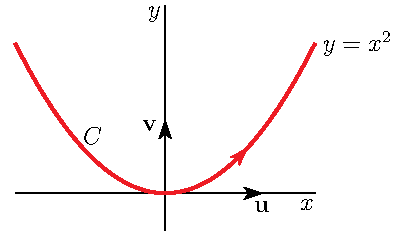
\includegraphics{OE16A_6h.pdf}
\end{center}

The curve $\big(a(t),b(t)\big)=(t,t^2)$ is the curve $y=x^2$.
It is ``curviest'' at the origin, which is consistent with part (f).
It becomes flatter and flatter as $|t|$ increases, but never achieves
``perfect flatness'', which is consistent with (g).


\end{answer}

\begin{solution} (a)
As
\begin{align*}
\vr(t) = 2t\hi + t^2\hj + \sqrt{3} t^2\hk \\
\vr'(t) = 2\hi + 2t\hj + 2\sqrt{3} t\hk 
%\vr'(t) =  2\hj + 2\sqrt{3}\hk
\end{align*}
the unit tangent vector is
\begin{align*}
\hat\vT(t) &=\frac{\hi + t\hj + \sqrt{3} t\hk }{|\hi + t\hj + \sqrt{3} t\hk |}
=\frac{\hi + t\hj + \sqrt{3} t\hk }{\sqrt{1+4t^2}}
\end{align*}


\noindent (b)
Since
\begin{align*}
\diff{\hat\vT}{t}(t)
&=\frac{ \hj + \sqrt{3} \hk }{\sqrt{1+4t^2}}
-4t\frac{\hi + t\hj + \sqrt{3} t\hk }{{(1+4t^2)}^{3/2}}
=\frac{-4t\hi + \hj + \sqrt{3} \hk }{{(1+4t^2)}^{3/2}}
\end{align*}
the unit normal is
\begin{align*}
\hat\vN(t) &=\frac{-4t\hi + \hj + \sqrt{3} \hk }
           {|-4t\hi + \hj + \sqrt{3} \hk|}
=\frac{-4t\,\hi + \hj + \sqrt{3} \hk }{2\sqrt{1+4t^2}}
\end{align*}

\noindent (c) 
The unit binormal is
\begin{align*}
\hat\vB(t) &= \hat\vT(t)\times \hat\vN(t) \\
&=\frac{1}{2(1+4t^2)}\det\left[\begin{matrix}
           \hi &  \hj & \hk \\
           1   &   t  &\sqrt{3} t \\
           -4t &   1  &\sqrt{3}
\end{matrix}\right] \\
&=\frac{-\sqrt{3}(1+4t^2)\hj  + (1+4t^2)\hk}{2(1+4t^2)} \\
&=-\frac{\sqrt{3}}{2}\hj +\frac{1}{2}\hk
\end{align*}
which is \textcircled{3}.

\noindent (d)
The plane contains the point $\vr(0)=\vZero$ and is perpendicular to the
vector $-\frac{\sqrt{3}}{2}\hj +\frac{1}{2}\hk$ and so is
\begin{equation*}
-\sqrt{3} y + z=0
\end{equation*}

\noindent (e)
The curvature is
\begin{align*}
\ka(t) &= \Big|\diff{\hat\vT}{t}(t)\Big|/\Big|\diff{s}{t}\Big|
=\frac{|-4t\hi + \hj + \sqrt{3} \hk| }{{(1+4t^2)}^{3/2}}
  \frac{1}{|2\hi + 2t\hj + 2\sqrt{3} t\hk |} \\
&=\frac{\sqrt{4+16t^2}}{{(1+4t^2)}^{3/2}}  \frac{1}{2\sqrt{1+4t^2}}
=\frac{1}{{(1+4t^2)}^{3/2}}
\end{align*}

\noindent (f), (g)
The denominator ${(1+4t^2)}^{3/2}$ of $\ka(t)$ is a minimum at $t=0$ and grows
without bound as $|t|$ increases. So the denominator never achieves
a maximum. Consquently, the curvature $\ka(t)$ achieves its
maximum value when $t=0$ and so at $\vr(0)=(0,0,0)$. The curvature
never achieves a minimum.

\noindent (h)
Since 
$\sqrt{3}\,\vv+\vw=4\,\hk$ and $\vv-\sqrt{3}\,\vw=4\,\hj$,
\begin{equation*}
\hi=\frac{\vu}{2}\qquad
\hj=\frac{\vv-\sqrt{3}\,\vw}{4}\qquad
\hk=\frac{\sqrt{3}\,\vv+\vw}{4}
\end{equation*}
Since $\vu=2\,\hi$ and $\vv=\hj+\sqrt{3}\,\hk$,
\begin{align*}
\vr(t) = t\,\vu + t^2 \,\vv
= a(t)\vu + b(t)\vv + c(t)\vw
\qquad\text{ with }a(t)=t,\ b(t)=t^2,\ c(t)=0
\end{align*}
The curve $\big(a(t),b(t)\big)=(t,t^2)$ is the curve $y=x^2$.
It is ``curviest'' at the origin, which is consistent with part (f).
It becomes flatter and flatter as $|t|$ increases, but never achieves
``perfect flatness'', which is consistent with (g).

\begin{center}
       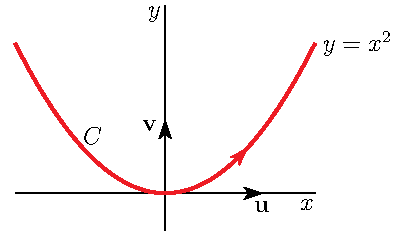
\includegraphics{OE16A_6h.pdf}
\end{center}

\intremark{
Aside from an overall factor of $\frac{1}{2}$, the change of coordinates
is orthogonal.
}


\end{solution}



%%%%%%%%%%%%%%%%%%%%%%%%%%%%%%%
\begin{question}[M317 2017D] %5
Recall that if $\hat\vT$ is the unit tangent vector to an oriented curve 
with arclength parameter $s$, then the curvature $\ka$ and the principle
normal vector $\hat\vN$ are defined by the equation
\begin{equation*}
\diff{\hat\vT}{s} = \ka\,\hat\vN
\end{equation*}
Moreover, the torsion $\tau$ and the binormal vector $\hat\vB$ are defined by
the equations
\begin{equation*}
\hat\vB = \hat\vT\times\hat\vN,\qquad
\diff{\hat\vB}{s} = -\tau\,\hat\vN
\end{equation*} 
Show that
\begin{equation*}
\diff{\hat\vN}{s} = -\ka\,\hat\vT + \tau\,\hat\vB
\end{equation*}
\end{question}

\begin{hint} 
Differentiate $\hat\vN =\hat\vB\times\hat\vT$ with respect to $s$. 

The vectors $\hN, \hB,$ and $\hT$ form a right-handed triple. Sketch them (the same way you might sketch the $x$, $y$, and $z$ axes) to figure out the signs of their cross products.
\end{hint}

\begin{answer} 
See the solution.
\end{answer}

\begin{solution} 
The three unit vectors $\hat\vT$, $\hat\vN$ and $\hat\vB$ are 
mutually perpendicular and form a right handed triple.
\begin{center}
     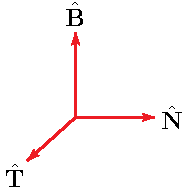
\includegraphics{OE17D_5.pdf}
\end{center}
So
\begin{equation*}
\hat\vN = \hat\vB\times\hat\vT \qquad
\hat\vN\times\hat\vT = -\hat\vB \qquad
\hat\vB\times\hat\vN = -\hat\vT
\end{equation*}
and
\begin{align*}
\diff{\hat\vN}{s} & = \diff{\hat\vB}{s}\times\hat\vT
                     +\hat\vB\times \diff{\hat\vT}{s}
= -\tau\,\hat\vN\times\hat\vT
                     +\hat\vB\times\big(\ka\hat\vN\big)
= \tau\,\hat\vB - \ka\hat\vT
\end{align*}
\end{solution}


%%%%%%%%%%%%%%%%%%%%%%%%%%%
\begin{question}[M317 2000D] %1
 A skier descends the hill $z =\sqrt{4-x^2-y^2}$ along a trail with 
parameterization
$$
x=\sin(2\theta),\qquad y=1-\cos(2\theta),\qquad z=2\cos\theta,\qquad
 0\le\theta\le\frac{\pi}{2}
$$
   Let $P$ denote the point on the trail where $x = 1$.
\begin{enumerate}[(a)]
\item
   Find the vectors $\hat\vT, \hat\vN, \hat\vB$ and 
   the curvature $\ka$ of the ski trail at the point $P$.
                                                         
\item
The skier's acceleration at $P$ is $\va = (-2, 3, -2\sqrt{2})$.
           Find, at $P$,
\begin{enumerate}[(i)]
\item
the rate of change of the skier's speed and
\item
the skier's velocity (a vector).
\end{enumerate}
\end{enumerate}

\end{question}

\begin{hint} 
In part (b), note that $\va$ is the second derivative with respect
       to time (not $\theta$). Exploit $\va = \diff{v}{t}\hat\vT + v^2\kappa\hat\vN$ to  find what you're asked for.
\end{hint}

\begin{answer} 
(a) $\hat\vT = \frac{1}{\sqrt6}\big(0,2,-\sqrt2\big)$,
    $\hat\vN = -\frac{1}{\sqrt{39}}\big(6,1,\sqrt2\big)$,
    $\hat\vB = \frac{1}{\sqrt{13}}\big(-1,2,2\sqrt2\big)$,
    $\kappa = \frac{\sqrt{13}}{3\sqrt3} = \frac{\sqrt{39}}{9}$

(b) (i) $\diff{v}{t}=\frac{5\sqrt2}{\sqrt3}$\qquad (ii) $\vv = (0,\sqrt2,-1)$.
\end{answer}

\begin{solution} (a)
Parametrizing the curve by $\theta$ gives
\begin{align*}
\vr(\theta) &= \big(\sin(2\theta),1-\cos(2\theta),2\cos\theta\big),
\\
\vv =\vr'(\theta)&= \big(2\cos(2\theta),2\sin(2\theta),-2\sin\theta\big),
\\
\va = \vr''(\theta)&=\big(-4\sin(2\theta),4\cos(2\theta),-2\cos\theta\big).
\end{align*}
At the point $P$, we have $\theta=\pi/4$, giving instantaneous
values
$$
\vr = (1,1,\sqrt2),
\quad
\vv = \big(0,2,-\sqrt2\big),
\quad
v = |\vv| = \sqrt6,
\quad
\va = \big(-4,0,-\sqrt2\big).
$$
Hence $\hat\vT = \frac{\vv}{|\vv|} 
   = \frac{1}{\sqrt6}\big(0,2,-\sqrt2\big)$.


Now $\hat\vB = \frac{\vv\times\va}{|\vv\times\va|}
%= \frac{1}{\sqrt{26}}\big(-2\sqrt2,4\sqrt2,8\big)
= \frac{1}{\sqrt{26}}\big(-\sqrt2,2\sqrt2,4\big)
= \frac{1}{\sqrt{13}}\big(-1,2,2\sqrt2\big)$,
since
$$
\vv\times\va
= \left|\begin{matrix}\hi & \hj & \hk \\
0 & 2 & -\sqrt2 \\
-4 & 0 & -\sqrt2 \end{matrix}\right|
= \big(-2\sqrt2,4\sqrt2,8\big),
\qquad
|\vv\times\va| = \sqrt{104} = 2\sqrt{26}.
$$
This leads to
$$
\hat\vN = \hat\vB\times\hat\vT
=\frac{1}{\sqrt{78}} \left|\begin{matrix}\hi & \hj & \hk \\
-1 & 2 & 2\sqrt2 \\
0  & 2 & -\sqrt2 \end{matrix}\right|
= -\frac{1}{\sqrt{78}}\big(6\sqrt2,\sqrt2,2\big)
= -\frac{1}{\sqrt{39}}\big(6,1,\sqrt2\big).
$$
Finally,
$$
\kappa = \frac{|\vv\times\va|}{v^3}
= \frac{2\sqrt{26}}{{(\sqrt{6})}^3} 
= \frac{2\sqrt2\,\sqrt{13}}{6\sqrt2\sqrt3}
= \frac{\sqrt{13}}{3\sqrt3} = \frac{\sqrt{39}}{9}.
$$

(b)
Now parametrize the curve by time, $t$, and write $\vv=\vr'(t)$,
$v=|\vr'(t)|$ and $\va=\vr''(t)$. Note that in part (a) we used
$\vv$, $v$ and $\va$ with different meanings.
We use the dot product to extract
the tangential and normal components of
$\va = \diff{v}{t}\hat\vT + v^2\kappa\hat\vN$:
\begin{align*}
	\va\cdot \hT &= \left(\diff{v}{t}\hat\vT + v^2\kappa\hat\vN\right)\cdot \hT\\
	&=\diff{v}{t}\hT\cdot\hT+(v^2\kappa)\hN\cdot\hT
	\intertext{Since $\hT$ is a unit vector, $\hT \cdot \hT=\|\hT\|^2=1$; since $\hT$ and $\hN$ are perpendicular, $\hT \cdot \hN =0$.}
	&=\diff{v}{t}
	\intertext{This gives us a nice way to compute $\diff{v}{t}$, the rate of change of speed.}
\diff{v}{t} &= \va\cdot\hat\vT
= (-2,3,-2\sqrt2)\cdot\frac{1}{\sqrt6}\big(0,2,-\sqrt2\big)\\
&= \frac{1}{\sqrt6}[0 + 6 + 4] = \frac{10}{\sqrt6} = \frac{5}{3}\sqrt6.
	\end{align*}

Similarly, $\va\cdot\hat\vN = v^2\kappa$, so
$$
v^2 
= \frac{1}{\kappa}\va\cdot\hat\vN
= \frac{9}{\sqrt{39}}\frac{-1}{\sqrt{39}}(-2,3,-2\sqrt2)
               \cdot\big(6,1,\sqrt2\big)
%= \frac{-9}{39}[-6+6-2]
= \frac{9\times 13}{39}
= 3.
$$
Hence $|v|=\sqrt{3}$; since $v=|\vv|$, $v=\sqrt3$. Then
$\vv = |\vv|\hT=v\hat\vT = \frac{\sqrt{3}}{\sqrt{6}}\big(0,2,-\sqrt2\big) = (0,\sqrt2,-1)$.
\end{solution}



%%%%%%%%%%%%%%%%%%%%%%%%%%%%%%%
\begin{question}[M317 2011A] %2
	A particle moves so that its position vector is given by 
	$\vr(t) = \big(\cos t\,,\, \sin t\,,\, c \sin t\big)$, where $t > 0$
	and $c$ is a constant.
	\begin{enumerate}[(a)]
		\item
		Find the velocity $\vv(t)$ and the acceleration $\va(t)$ of the particle.
		\item
		Find the speed $v(t)=|\vv(t)|$ of the particle.
		\item
		Find the tangential component of the acceleration of the particle.
		\item
		Show that the trajectory of this particle lies in a plane.
	\end{enumerate}
\end{question}

\begin{hint} 
	For part (d), what is the relationship between the $y$- and $z$-components of the particle's position? How can you use that to find a plane containing the particle at all times $t$?
\end{hint}

\begin{answer} 
	(a) $\vv(t) = \big(-\sin t\,,\, \cos t\,,\, c \cos t\big)$, 
	$\va(t) = \big(-\cos t\,,\, -\sin t\,,\, -c \sin t\big)$
	
	(b) $v(t) = \sqrt{1+c^2\cos^2 t}$\qquad
	(c) $\frac{-c^2\sin t\cos t}{\sqrt{1+c^2\cos^2 t}}$
	
	(d) The curve lies on the plane $z=cy$.
\end{answer}

\begin{solution} 
	(a) The position, velocity and acceleration are
	\begin{align*}
	\vr(t) &= \big(\cos t\,,\, \sin t\,,\, c \sin t\big) \\
	\vv(t) =\vr'(t) &= \big(-\sin t\,,\, \cos t\,,\, c \cos t\big) \\
	\va(t) =\vr''(t)&= \big(-\cos t\,,\, -\sin t\,,\, -c \sin t\big) 
	\end{align*}
	
	(b) The speed is
	\begin{align*}
	v(t) = |\vv(t)| = \sqrt{1+c^2\cos^2 t}
	\end{align*}
	
	(c) By Theorem \eref{CLP317}{thm:curvatureFormulae}.c in the CLP-4 text,
	the tangential component of the acceleration is
	\begin{align*}
	\difftwo{s}{t} = \diff{\hfill}{t} \sqrt{1+c^2\cos^2 t}
	= \frac{-c^2\sin t\cos t}{\sqrt{1+c^2\cos^2 t}}
	\end{align*}
	
	(d) $y(t) =\sin t$ and $z(t) = c\sin t$ obey
	$z(t) = cy(t)$ for all $t$. So the curve lies on the  plane $z=cy$.
\end{solution}
%%%%%%%%%%%%%%%%%%%%%%%%%%%
\begin{question}[M317 2017A] %3
	A race track between two hills is described by the parametric curve
	\begin{equation*}
	\vr(\theta) = \Big(4 \cos\theta\,,\, 2\sin\theta\,,\, 
	\frac{1}{4}\cos(2\theta)\Big),\qquad
	0 \le \theta \le 2\pi
	\end{equation*}
	\begin{enumerate}[(a)]
		\item
		Compute the curvature of the track at the point $\big(-4, 0, \frac{1}{4}\big)$.
		
		\item
		Compute the radius of the circle that best approximates the bend at the
		point\\ $\big(-4, 0, \frac{1}{4}\big)$ (that is, the radius of the 
		osculating circle at that point).
		
		\item
		A car drives down the track so that its position at time $t$ is given by
		$\vr(t^2)$. (Note the relationship between $t$ and $\theta$ is $\theta = t^2$). 
		Compute the following quantities.
		\begin{enumerate}[(i)]
			\item
			The speed at the point $\big(-4, 0, \frac{1}{4}\big)$.
			\item
			The acceleration at the point $\big(-4, 0, \frac{1}{4}\big)$.
			
			\item
			The magnitude of the normal component of the acceleration at the point\\
			$\big(-4, 0, \frac{1}{4}\big)$.
		\end{enumerate}
	\end{enumerate}
\end{question}

\begin{hint} 
	Rather than trying to wrangle trig identities, plug in $\theta=\pi$ as soon as you can for part (a). For part (c), remember that you need the chain rule if you want to make use of your previous derivatives.
\end{hint}

\begin{answer} 
	(a) $\frac{\sqrt{17}}{4}$\qquad
	(b) $\frac{4}{\sqrt{17}}$\qquad
	(c) (i) $4\sqrt{\pi} $\quad
	(ii) $\big( 16\pi\,,\, -4\,,\, -4\pi\big)$\quad
	(iii) $4\sqrt{17}\,\pi$
\end{answer}

\begin{solution} (a) 
	For the specified curve $\vr(\pi) = \big(-4,0,\frac{1}{4}\big)$ and
	\begin{align*}
	\vr(\theta) &= \Big(4 \cos\theta\,,\, 2\sin\theta\,,\, 
	\frac{1}{4}\cos(2\theta)\Big) \\
	\vv(\theta)=\vr'(\theta) &= \Big(-4 \sin\theta\,,\, 2\cos\theta\,,\, 
	-\frac{1}{2}\sin(2\theta)\Big) \\
	\va(\theta) = \vr''(\theta) &= \Big(-4 \cos\theta\,,\, -2\sin\theta\,,\, 
	-\cos(2\theta)\Big) \\
	\vv(\pi) &= \big(0\,,\, -2\,,\, 0\big) \\
	\va(\pi) &= \big(4\,,\, 0\,,\, -1\big) \\
	\vv(\pi) \times \va(\pi) &= \big(2\,,\, 0\,,\, 8\big) 
	\end{align*}
	So the curvature at $\theta=\pi$ is
	\begin{align*}
	\ka(\pi)&=\frac{|\vv(\pi) \times \va(\pi)|}{|\vv(\pi)|^3}
	=\frac{|(2,0,8)|}{|(0,-2,0)|^3}
	=\frac{\sqrt{17}}{4}
	\end{align*}
	
	(b) The radius is
	\begin{equation*}
	\frac{1}{\ka(\pi)} = \frac{4}{\sqrt{17}}
	\end{equation*}
	
	(c) Set $\vR(t) = \vr(t^2)$. Then 
	\begin{align*}
	\vR'(t)&=2t\,\vr'(t^2)  \\
	\vR''(t) &= 2\,\vr'(t^2) +4t^2\,\vr''(t^2) 
	\end{align*}
	In particular,
	\begin{align*}
	\vR(\sqrt{\pi}) &= \Big(-4\,,\, 0\,,\,  \frac{1}{4}\Big) \\
	\vR'(\sqrt{\pi}) &= 2\sqrt{\pi}\,\vv(\pi)
	=\big(0\,,\, -4\sqrt{\pi}\,,\, 0\big) \\
	\text{speed} = \big|\vR'(\sqrt{\pi})\big| &=4\sqrt{\pi} \\
	\text{acceleration}=\vR''(\sqrt{\pi})
	&= 2\,\vv(\pi)+4\pi\,\va(\pi)
	= \big( 16\pi\,,\, -4\,,\, -4\pi\big) 
	\end{align*}
	%\begin{align*}
	%\vR(t) =\vr(t^2) &= \Big(4 \cos t^2\,,\, 2\sin t^2\,,\, 
	%                                  \frac{1}{4}\cos(2 t^2)\Big) \\
	%\vR'(t)=2t\,\vr'(t^2) &= \Big(-8 t\sin t^2\,,\, 4t\cos t^2\,,\, 
	%                                  -t\sin(2 t^2)\Big) \\
	%\vR''(t) &= 2\,\vr'(t^2) +4t^2\,\vr''(t^2) \\
	%   &= \Big(-8\sin t^2 -16t^2 \cos t^2\,,\, 
	%            4\cos t^2-8t^2\sin t^2\,,\, 
	%            -\sin(2 t^2) -4t^2 \cos(2t^2)\Big) 
	%\end{align*}
	%In particular,
	%\begin{align*}
	%\vR(\sqrt{\pi}) &= \Big(-4\,,\, 0\,,\,  \frac{1}{4}\Big) \\
	%\vR'(\sqrt{\pi}) &= \big(0\,,\, -4\sqrt{\pi}\,,\, 0\big) \\
	%\text{speed} = \big|\vR'(\sqrt{\pi})\big| &=4\sqrt{\pi} \\
	%\text{acceleration}=\vR''(\sqrt{\pi}) 
	%   &= \big( 16\pi\,,\, -4\,,\, -4\pi\big) 
	%\end{align*}
	The normal component of the acceleration has magnitude
	\begin{align*}
	\ka\Big(\diff{s}{t}\Big)^2 = \frac{\sqrt{17}}{4}\big(4\sqrt{\pi}\big)^2
	=4\sqrt{17}\,\pi
	\end{align*}
\end{solution}
\setcounter{section}{5}
%\section{A Compendium of Curve Formula}
%\input{problems/prob_s1.5}
\section{Integrating Along a Curve}
%\documentclass[12pt]{article}

\questionheader{ex:s1.6}

%%%%%%%%%%%%%%%%%%
\subsection*{\Conceptual}
%%%%%%%%%%%%%%%%%%
%%%%%%%%%%%%%%%%%%%
%%%%%%%%%%%%%%%
%%%%%%%%%%%%%%%%%%%
\begin{question}
Give an equation for arclength of a curve $C$ as a line integral.
\end{question}
\begin{hint}
Your differential is $\dee{s}$, where $s$ is arclength.
\end{hint}
\begin{answer}
$\int_C \dee{s}$
\end{answer}
\begin{solution}
We want to add up all the tiny pieces of arclength $\dee{s}$ along a curve $C$. So, the integral would simply be $\int_C \dee{s}$.

To see this another way, if we define $\vr=(x(t),y(t),z(t))$ for $a \le t \le b$ to be the equation of $C$, we could calculate the arclength as:
\begin{align*}
\int_a^b |\vr'(t)|\dee{t}&=\int_a^b \sqrt{x'(t)^2+y'(t)^2+z'(t)^2}\dee{t}
\end{align*}
This fits the form of Definition~\eref{CLP317}{def:lineIntegral} with $f(x,y,z)=1$, so we write it as a line integral as $\int_C 1 \dee{s}$, which is equivalent to $\int_C \dee{s}$.
\end{solution}


%%%%%%%%%%%%%%%%%%%
\begin{question}
\begin{enumerate}[(a)]
\item
Show that the integral $\int_\cC f(x,y)\,ds$ 
along the curve $\cC$ given in polar coordinates by 
$r=r(\theta)$, $\theta_1\le \theta\le\theta_2$, is
\begin{equation*}
\int_{\theta_1}^{\theta_2}f\big(r(\theta)\cos\theta, r(\theta)\sin\theta\big) \sqrt{r(\theta)^2+\left(\diff{r}{\theta}(\theta)\right)^2}\,
\dee{\theta}
\end{equation*}

\item
Compute the arc length of $r=1+\cos\theta,\ 0\le \theta\le 2\pi$.
You may use the formula
\begin{equation*}
1+\cos\theta=2\cos^2\frac{\theta}{2}
\end{equation*}
to simplify the computation.	
\end{enumerate}
\end{question}

\begin{hint}
(a) You can parametrize the curve by 
   $\vr(\theta) = r(\theta)\,\cos\theta\,\hi +
                  r(\theta)\,\sin\theta\,\hj$, $\theta_1\le \theta\le\theta_2$.
\end{hint}

\begin{answer}
(a) See the solution.\qquad
(b) $8$
\end{answer}

\begin{solution}
(a) The curve is 
$\vr(\theta) = x(\theta)\,\hi+ y(\theta)\,\hj$
with $x(\theta)=r(\theta)\cos\theta$, $y(\theta)=r(\theta)\sin\theta$ 
and $\theta_1\le \theta\le \theta_2$.
On this curve 
\begin{align*}
\vv(\theta) =\diff{\vr}{\theta}(\theta)&= x'(\theta)\hi+ y'(\theta)\hj
=\big[r'(\theta)\cos\theta-r(\theta)\sin\theta\big]\hi+
\big[r'(\theta)\sin\theta+r(\theta)\cos\theta\big]\hj\cr
\implies  \diff{s}{\theta}(\theta)
&=\sqrt{\big[r'(\theta)\cos\theta-r(\theta)\sin\theta\big]^2
+ \big[r'(\theta)\sin\theta+r(\theta)\cos\theta\big]^2}\cr
&=\sqrt{r'(\theta)^2+r(\theta)^2}
\end{align*}
Hence
\begin{align*}
\int_\cC f(x,y)\,ds 
&= \int_{\theta_1}^{\theta_2}\!\!\!f\big(x(\theta), y(\theta)\big) \diff{s}{\theta}\,\dee{\theta}
\cr
&=\int_{\theta_1}^{\theta_2}\!\!\!f\big(r(\theta)\cos\theta, r(\theta)\sin\theta\big) \sqrt{r(\theta)^2
     +\left(\diff{r}{\theta}(\theta)\right)^2}\,
\dee{\theta}
\end{align*}

(b)
In this case $f(x,y)=1$, $r(\theta)=1+\cos\theta$, $\theta_1=0$ and $\theta_2=2\pi$,
\begin{align*}
\int_C \,ds
&=\int_0^{2\pi} \sqrt{[1+\cos\theta]^2+[-\sin\theta]^2}\,\dee{\theta}
=\int_0^{2\pi} \sqrt{2(1+\cos\theta)}\,\dee{\theta}\cr
&=\int_0^{2\pi} \sqrt{4\cos^2\frac{\theta}{2}}\,\dee{\theta}
=2\int_0^{2\pi} \left|\cos\frac{\theta}{2}\right|\,\dee{\theta}
=4\int_0^{\pi} \cos\frac{\theta}{2}\ \dee{\theta}
=8 \sin\frac{\theta}{2}\bigg|_0^{\pi}
=8
\end{align*}
\end{solution}

%%%%%%%%%%%%%%%%%%%
%\begin{question}
%Evaluate $\int_\cC x^2y^2\,\dee{x}$ along the line segment from 
%$(0,1)$ to $(1,1)$. (When we move to the right from $(x,1)$ to $(x+\dee{x},1)$
%with $\dee{x}>0$, the distance moved is $\dee{s}=\dee{x}$. So in this case, 
%it is common to write
%$\int_\cC x^2y^2\,\dee{x}$ in place of $\int_\cC x^2y^2\,\dee{s}$.)
%\end{question}
%
%\begin{hint}
%The line segement $\cC$ can be easily parameterized using $x$
%as the parameter. 
%\end{hint}
%\begin{answer}
%$\frac{1}{3}$
%\end{answer}
%\begin{solution}
%We may parametrize $\cC$ by $\vr(x)=x\,\hi+\hj$ with $0\le x\le 1$.
%So $\big|\diff{\vr}{x}(x)\big| = |\hi|=1$ and 
%\begin{align*}
%\int_\cC x^2y^2\,\dee{x}
%&=\int_0^1 x^2 \overbrace{(1)^2}^{y^2}\ \left|\diff{\vr}{x}(x)\right|\,\dee{x} \\
%&=\int_0^1 x^2 \,\dee{x} \\
%&=\frac{1}{3}
%\end{align*}
%
%\end{solution}


%%%%%%%%%%%%%%%%%%%
%%%%%%%%%%%%%%%%%%%


%%%%%%%%%%%%%%%%%%%

%%%%%%%%%%%%%%%%%%
\subsection*{\Procedural}

%%%%%%%%%%%%%%%%%%%%%%%%%
\begin{question}
Calculate $\int_C \left(\frac{xy}{z}\right)\dee{s}$, where $C$ is the curve $\left( \frac23t^3~,~\sqrt{3}t^2~,~3t \right)$ from $t=1$ to $t=2$.
\end{question}
\begin{hint}
Following Definition~\eref{CLP317}{def:lineIntegral}, set $f(x,y,z)=\frac{xy}{z}$, $x(t)=\frac23 t^3$, $y(t)=\sqrt3t^2$, and $z(t)=3t$.
\end{hint}
\begin{answer}
$ \frac{4}{21\sqrt 3}(2^7-1) + \frac{2}{5\sqrt 3}(2^5-1)$
\end{answer}
\begin{solution}
Following Definition~\eref{CLP317}{def:lineIntegral}:
\begin{align*}
\int_C \left(\frac{xy}{z}\right)\dee{s}&=\int_1^2 \left(\frac{\frac23t^3 \cdot \sqrt{3}t^2}{ 3t} \right)\sqrt{(2t^2)^2+(2\sqrt3 t)^2+(3)^2}\,\dee{t}\\
&=\int_1^2 \left(\frac{2}{ 3\sqrt 3} \,t^4\right)(2t^2+3)\,\dee{t} = \frac{4}{21\sqrt 3}(2^7-1) + \frac{2}{5\sqrt 3}(2^5-1)
\end{align*}
\end{solution}
%%%%%%%%%%%%%%%%%%%%%%%%%%%%%%%
%%%%%%%%%%%%%%%%%%%
\begin{question}
	A hoop of radius $r$ traces out the curve $x^2+y^2=1$, where $x$ and $y$ are measured in metres. At a point $(x,y)$, its density is $x^2$ kg per metre. What is the mass of the hoop?
\end{question}
\begin{hint}
	Parametrize the circle in the usual way.
\end{hint}
\begin{answer}
	$\pi$ kg
\end{answer}
\begin{solution}
	We parametrize the unit circle as $(\cos t, \sin t)$, $0 \le t \le 2\pi$.
	
		A tiny slice of the hoop with length $\dee{s}$ has mass $(x^2~ \mathrm{kg}/\mathrm{m})(\dee{s}~ \mathrm{m})=x^2\dee{s}~ \mathrm{kg}$. So, the entire hoop has mass:
		\begin{align*}
			\int_C x^2\,\dee{s}&=\int_0^{2\pi} \cos^2 t \sqrt{(-\sin t)^2+(\cos t)^2}\,\dee{t}=\int_0^{2\pi} \cos^2 t \,\dee{t}\\
&=\int_0^{2\pi} \frac{1+\cos(2t)}{2}\ \dee{t}
                 =\left[\frac{t}{2} +\frac{\sin(2t)}{4} \right]_0^{2\pi}=\pi ~\mathrm{kg}
			\end{align*}
			 For an efficient, sneaky, way to evaluate 
                 $\int_0^{2\pi} \cos^2 t\ \dee{t}$, see Example
                 \eref{CLP317}{eg:workIntegalB} in the CLP-4 text.
\end{solution}

%%%%%%%%%%%%%%%%%%%
\begin{question}
	Compute $\int_C (xy+z) \dee{s}$ where $C$ is the straight line from $(1,2,3)$ to $(2,4,5)$.
\end{question}
\begin{hint}
	$C$ can be parametrized as $(1+t,2+2t,3+2t)$ for $0 \le t \le 1$.
\end{hint}
\begin{answer}
	$26$
\end{answer}
\begin{solution}
	To parametrize $C$, we note the vector between the two points is $(2-1,4-2,5-3)=(1,2,2)$. So, the line is $(1,2,3)+t(1,2,2)$ for $0 \le t \le 1$. That is, $x(t)=1+t$, $y(t)=2+2t$, and $z(t)=3+2t$.
	\begin{align*}
		\int_C(xy+z)\dee{s}&=\int_0^1 \left((1+t)(2+2t)+(3+2t)\right)\sqrt{1^1+2^2+2^2}\dee{t}\\
		&=              \int_0^1 3\big(5 + 6t + 2t^2\big)\ \dee{t}=26
		\end{align*}
\end{solution}


%%%%%%%%%%%%%%%%%%%
\begin{question}
Evaluate the path integral $\int_\cC f(x,y,z)\,\dee{s}$ for
\begin{enumerate}[(a)]
\item 
$f(x,y,z)=x\cos z$, \ \ \ $\cC:\vr(t)=t\hi+t^2\hj$,
$0\le t\le 1$.

\item $f(x,y,z)=\frac{x+y}{y+z}$, \ \ \ \ \ \ 
$\cC:\vr(t)= \big(t,\frac{2}{3}t^{3/2},t\big)$,
$1\le t\le 2$.	
\end{enumerate}
\end{question}

%\begin{hint}
%\end{hint}

\begin{answer}
(a) $\frac{5^{3/2}-1}{12}$\qquad
(b) $\frac{8-3^{3/2}}{3/2}$	
\end{answer}

\begin{solution}
(a) 
In this case $\vr(t)=t\hi+t^2\hj$, so that
$\vv(t)=\diff{\vr}{t}(t)=\hi+2t\hj$ and $\diff{s}{t}=\sqrt{1+4t^2} $. Hence
\begin{align*}
\int_\cC f(x,y,z)\,\dee{s}
&=\int_0^1 x(t)\cos z(t) \diff{s}{t}\,\dee{t}
=\int_0^1 t(\cos 0) \sqrt{1+4t^2}\,\dee{t}
=\frac{1}{8}\frac{ {(1+4t^2)}^{3/2}}{3/2}\bigg|_0^1\\
&=\frac{5^{3/2}-1}{12}
\end{align*}

(b) In this case $\vr(t)=\big(t,\frac{2}{3}t^{3/2},t\big)$, so
that
$\vv(t)=\diff{\vr}{t}(t)=\big(1,t^{1/2},1\big)$ and 
$\diff{s}{t}=\sqrt{2+t} $. Hence
\begin{align*}
\int_\cC f(x,y,z)\,\dee{s}
&=\int_1^2 \frac{x(t)+y(t)}{y(t)+z(t)} \, \diff{s}{t}\,\dee{t}
=\int_1^2 \frac{t+{2\over 3}t^{3/2}}{{2\over3}t^{3/2}+t} \sqrt{2+t}\,\dee{t}
=\frac{(2+t)^{3/2}}{3/2}\bigg|_1^2 \\
&=\frac{8-3^{3/2}}{3/2}
\end{align*}	

\end{solution}



%%%%%%%%%%%%%%%%%%%%%%%%%
\begin{question}
	Evaluate $\int_C \sin x\,\dee{s}$, where $C$ is the curve $(\arcsec(t), \ln t)$, $1 \le t \le \sqrt{2}$. 
\end{question}
\begin{hint}
	Simplify! Also: $\diff{}{t}\{\arcsec t\} = \frac{1}{|t|\sqrt{t^2-1}}$.
\end{hint}
\begin{answer}
	$\frac12 \ln 2$
\end{answer}
\begin{solution}
  In the figure below, we construct a triangle with $\theta=\arcsec t$; the hypotenuse has length $t$, while the side adjacent to $\theta$ has length 1. By the Pythagorean Theorem, the remaining side has length $\sqrt{t^2-1}$, so $\sin\theta=\sin(\arcsec t)=\frac{\sqrt{t^2-1}}{t}$.
               \begin{center}
\trigtri{\theta}{1}{\sqrt{t^2-1}}{t}\end{center}
Remember $\diff{}{t}\{\ln t\} = \frac{1}{t}$ and $\diff{}{t}\{\arcsec t\} = \frac{1}{|t|\sqrt{t^2-1}}$. In our range, $1 \le t \le \sqrt 2$, we have $|t|=t$.
	\begin{align*}
		\int_C \sin x \,\dee{s}&=\int_{1}^{\sqrt 2}\sin\left(\arcsec t \right)\sqrt{\left(\frac{1}{t\sqrt{t^2-1}} \right)^2+\left(\frac1t \right)^2}\,\dee{t}\\
		&=\int_1^{\sqrt{2}} \frac{\sqrt{t^2-1}}{t}\sqrt{\frac{1}{t^2(t^2-1)}+\frac{1}{t^2}} \,\dee{t}\\
		&=\int_1^{\sqrt 2}\frac1t\,\dee{t}=\frac{1}{2}\ln 2
	\end{align*}
\end{solution}


%%%%%%%%%%%%%%%%%%%%%%%%%%%%%%%
\begin{question}[M317 2012J] %3
A particle of mass $m = 1$ has position $\vr(0) = \hj$ and 
velocity $\vv_0 = \hi + \hk$ at time $t = 0$. The particle moves 
under a force 
\begin{equation*}
\vF(t) = \hj - \sin t\,\hk
\end{equation*}
where $t$ denotes time.
\begin{enumerate}[(a)]
\item
Find the position $\vr(t)$ of the particle as a function of $t$.
\item
Find the position $\vr(t_1)$ of the particle when it crosses the 
plane $x = \pi/2$ for the first time at $t_1$.
\item
Determine the work done by $\vF$ in moving the particle from $\vr(0)$ to 
$\vr(t_1)$.
\end{enumerate}
\end{question}

\begin{hint} 
Newton's law of motion is $\vF=m\va$. The work done over a displacement $\dee{\vr}$ is $W=\vF \cdot \dee{\vr}$.
\end{hint}

\begin{answer} 
(a) $\vr(t) = t\,\hi +\Big(1+\frac{t^2}{2}\Big)\,\hj + \sin t\,\hk$\qquad
(b) $\vr(\pi/2) = \frac{\pi}{2}\,\hi  +\Big(1+\frac{\pi^2}{8}\Big)\,\hj + \hk$
   \qquad
(c) $\frac{\pi^2}{8}-\frac{1}{2}$
\end{answer}

\begin{solution}
(a) Since the particle has mass $m=1$, Newton's law of motion 
$m\va=\vF$ simplifies to
\begin{equation*}
\vr''(t) = \hj - \sin t\,\hk
\end{equation*}
Integrating once gives
\begin{equation*}
\vr'(t) = t\,\hj + \cos t\,\hk + \mathbf{C}
\end{equation*}
for some constant vector $\mathbf{C}$.
To satisfy the initial condition that $\vr'(0) = \vv_0=\hi+\hk$, 
we need
\begin{align*}
\hi+\hk = \vr'(0) = \hk + \mathbf{C}
\implies \mathbf{C} = \hi
\end{align*}
So
\begin{equation*}
\vr'(t) %= t\,\hj +(\cos t-1)\,\hk +\vv_0
        = \hi + t\,\hj + \cos t\,\hk 
\end{equation*}
Integrating a second time, and imposing the initial condition that $\vr(0)
=\hj$, gives
\begin{equation*}
\vr(t)  = t\,\hi + \frac{t^2}{2}\,\hj + \sin t\,\hk +\hj
        = t\,\hi +\Big(1+\frac{t^2}{2}\Big)\,\hj + \sin t\,\hk
\end{equation*}

(b) The particle has $x(t) =\pi/2$ when $t=\pi/2$. So
\begin{equation*}
\vr(\pi/2) = \frac{\pi}{2}\,\hi  +\Big(1+\frac{\pi^2}{8}\Big)\,\hj + \hk
\end{equation*}

(c) The work done is
\begin{align*}
\text{Work} &= \int_0^{\pi/2} \vF(t)\cdot\vr'(t)\ \dee{t} \\
  &= \int_0^{\pi/2} \big(\hj - \sin t\,\hk\big)\cdot
         \big(\hi + t\,\hj + \cos t\,\hk\big)\ \dee{t} \\
  &= \int_0^{\pi/2} \big(t-\sin t\cos t\big)\,\dee{t} \\
  &= \Big[\frac{t^2}{2} +\frac{1}{2}\cos^2 t\Big]_0^{\pi/2} \\
  & = \frac{\pi^2}{8}-\frac{1}{2}
\end{align*}
\end{solution}



%%%%%%%%%%%%%%%%%%
\subsection*{\Application}
%%%%%%%%%%%%%%%%%%
%%%%%%%%%%%%%%%%%%%%%%%%%%%%%%%
\begin{question}[M317 2016D] %5
Evaluate the line integral $\int_C \vF\cdot\hn\,\dee{s}$ where
$\vF(x,y) = xy^2 \,\hi + ye^x \,\hj$ , $C$ is the boundary of the
rectangle $R$: $0 \le x \le 3$, $-1 \le y \le 1$, and  $\hn$ is the unit vector, normal to $C$, pointing to the outside of the rectangle.
\end{question}

\begin{hint} 
Sketch $C$ and determine the normal vectors from the sketch. You can use $x$ or $y$ as the integration variable in your 
           integrals.
\end{hint}

\begin{answer} 
$2e^3$
\end{answer}

\begin{solution} 
Here is a sketch of the rectangle $R$.

\begin{center}
     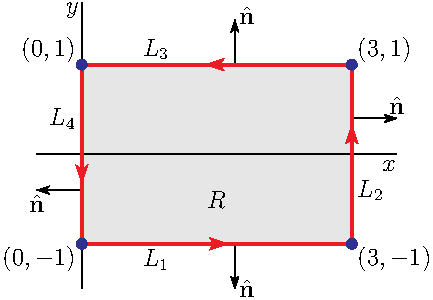
\includegraphics[scale=0.90]{OE16D_5.pdf}\
\end{center}

Its boundary consists of four line segments.
\begin{itemize}\itemsep1pt \parskip0pt \parsep0pt %\itemindent-15pt
\item[$\circ$]
$L_1$ from $(0,-1)$ to $(3,-1)$, with $\hn = -\hj$
\item[$\circ$]
$L_2$ from $(3,-1)$ to $(3,1)$, with $\hn = \hi$
\item[$\circ$]
$L_3$ from $(3,1)$ to $(0,1)$, with $\hn = \hj$
\item[$\circ$]
$L_4$ from $(0,1)$ to $(0,-1)$, with $\hn = -\hi$
\end{itemize}
So
\begin{align*}
\int_C \vF\cdot\hn\,\dee{s}
&= \int_{L_1} \vF\cdot(-\hj)\,\dee{s}
   +\int_{L_2} \vF\cdot \hi\,\dee{s}
   +\int_{L_3} \vF\cdot(\hj)\,\dee{s}
   +\int_{L_4} \vF\cdot(-\hi)\,\dee{s} \\
&= \int_0^3  -\overbrace{(-1)}^{y}e^x\,\dee{x}
   +\int_{-1}^1  \overbrace{(3)}^{x}y^2\,\dee{y}
   +\int^0_3  \overbrace{(1)}^{y}e^x\,\overbrace{(-\dee{x})}^{\dee{s}}
   +\int^{-1}_1  \overbrace{(0)}^{x}y^2\,\overbrace{(-\dee{y})}^{\dee{s}} \\
&=\big[e^3-1\big]+\big[1^3-(-1)^3\big] + \big[e^3-1\big]+0 \\
&=2e^3
\end{align*}
The trickiest part of this computation is getting $\dee{s}$ correct on
$L_3$ and $L_4$ (remembering that $\dee{s}$ is the arc length traveled
and so is positive, while $\dee{x}<0$ on $L_3$ and $\dee{y}<0$ on $L_4$).
To make a more detailed computation of $\int_{L_3} \vF\cdot(\hj)\,\dee{s}$,
parametrize $L_3$ by
\begin{equation*}
\vr(t) = (3,1) + t\big\{(0,1)-(3,1)\big\}
       = \big(3-3t,1\big)\qquad
0\le t\le 1
\end{equation*}
so that $\vr(0) = (3,1)$ is the initial point of $L_3$ and
$\vr(1) = (0,1)$ is the final point of $L_3$. Then
\begin{equation*}
\vr'(t) = (-3,0)\qquad
\diff{s}{t}(t) = |\vr'(t)| = 3
\end{equation*}
and
\begin{align*}
\int_{L_3} \vF\cdot \hj\,\dee{s}
=\int_0^1 \vF\big(\vr(t)\big)\cdot \hj\,\diff{s}{t}(t)\,\dee{t}
=\int_0^1\overbrace{e^{3-3t}}^{y(t)e^{x(t)}}\,
\overbrace{3}^{\diff{s}{t}(t)}\,\dee{t}
=-e^{3-3t}\Big|_0^1
=e^3-1
\end{align*}
\end{solution}


%%%%%%%%%%%%%%%%%%%%%%%%%%%%%%%
\begin{question}[M317 1998D] %1
	Let $\cC$ be the curve given by 
	$$
	\vr(t)=t\cos t\,\hi+t\sin t\,\hj+t^2\,\hk,\qquad 0\le t\le \pi
	$$
	\begin{enumerate}[(a)]
		\item
		Find the unit tangent $\hT$ to $\cC$ at the point $(-\pi,0,\pi^2)$.
		\item
		Calculate the line integral
		$$
		\int_\cC \sqrt{x^2+y^2}\ \dee{s}
		$$
		\item
		Find the equation of a smooth surface in $3$-space containing
		the curve $\cC$.
		\item
		Sketch the curve $\cC$.
	\end{enumerate}
\end{question}

\begin{hint} 
	(c) How is $x(t)^2+y(t)^2$ related to $z(t)$?
	
	(d) First, sketch $\big(x(t)\,,\,y(t)\big)$.
	
\end{hint}

\begin{answer} 
	(a) $\frac{1}{\sqrt{1+5\pi^2}}\big(-\hi-\pi\,\hj+2\pi\,\hk\big)$\qquad
	(b) $\frac{1}{15}\big[(1+5\pi^2)^{3/2}-1\big]$\qquad
	(c) $z=x^2+y^2$
	
	(d) 
	\begin{center}
		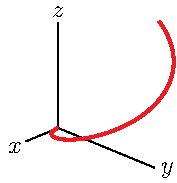
\includegraphics{OE98D_1.pdf}
	\end{center}
	
\end{answer}

\begin{solution} 
	(a) Since $\vr(t)=t\cos t\,\hi+t\sin t\,\hj+t^2\,\hk$
	\begin{align*}
		\vr'(t)&=\big(\cos t-t\sin t\big)\hi+\big(\sin t+t\cos t\big)\,\hj+2t\,\hk\\
		\diff{s}{t}
		&=|\vr'(t)|
		=\sqrt{\big(\cos t-t\sin t\big)^2+\big(\sin t+t\cos t\big)^2+(2t)^2}\\
		&=\sqrt{1+5t^2}\\
		\vr'(\pi)&=-\hi-\pi\,\hj+2\pi\,\hk\\
		\hat\vT(\pi)&=\frac{\vr'(t)}{|\vr'(t)|}
		=\frac{1}{\sqrt{1+5\pi^2}}\big(-\hi-\pi\,\hj+2\pi\,\hk\big)
	\end{align*}
	
	(b)
	\begin{align*}
		\int_\cC \sqrt{x^2+y^2}\ \dee{s}
		&=\int_0^\pi \sqrt{x^2(t)+y^2(t)}\ \diff{s}{t}\ \dee{t}
		=\int_0^\pi t\ \sqrt{1+5t^2}\ \dee{t}
		=\left[\frac{1}{15}(1+5t^2)^{3/2}\right]_0^\pi \\
		&=\frac{1}{15}\big[(1+5\pi^2)^{3/2}-1\big]
	\end{align*}
	
	(c) For every $t$, the coordinates $x(t)=t\cos t$, $y(t)=t\sin t$, 
	$z(t)=t^2$ obey $x(t)^2+y(t)^2= t^2 = z(t)$ and so the curve lies on
	$z=x^2+y^2$.
	
	(d) First concentrate on $\big(x(t)\,,\,y(t)\big)$. As $t$ runs from $0$
	to $\pi$, the curve $\big(r\cos t\,,\,r\sin t\big)$ sweeps out 
	half of a circle of radius $r$. Our  $\big(x(t)\,,\,y(t)\big)$
	does something similar, but the radius $r=t$ increases from $0$
	to $\pi$. Thus our $\big(x(t)\,,\,y(t)\big)$
	sweeps out the beginning of a spiral. At the same time $z(t)$
	increases from $0$ to $\pi^2$. So the curve $\cC$ looks like
	
	\begin{center}
		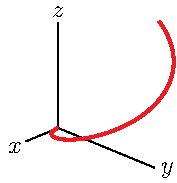
\includegraphics{OE98D_1.pdf}
	\end{center}
	
\end{solution}

%%%%%%%%%%%%%%%%%%%
\begin{question}
A wire traces out a path $C$  described by the curve $(t+\frac12t^2~,~t-\frac12t^2~,~\frac{4}{3}\,t^{3/2})$, $0 \leq t \leq 4$. Its density at the point $(x,y,z)$ is $\rho(x,y,z)={\left( \frac{x+y}{2}\right)}$. Find its centre of mass.
\end{question}
\begin{hint}
	Remember $\bar x = \dfrac{\int_C x\rho\,\dee{s}}{\int_C \rho\,\dee{s}}$, etc. The integrals you evaluate should all be straightforward applications of the power rule.
\end{hint}
\begin{answer}
	$\left( \frac{412}{55},-\frac{92}{55},\frac{4736}{693}\right)$
\end{answer}
\begin{solution}
We use the centre of mass formulae $\bar x = \dfrac{\int_C x\rho\,\dee{s}}{\int_C \rho\,\dee{s}}$, etc. To make the working clearer, we'll break these calculations into several steps.
\begin{align*}
x(t)&= t+ \frac12 t^2 & x'(t)&=1+t\\
y(t)&= t- \frac12 t^2 & y'(t)&=1-t\\
z(t)&=\frac43 t^{3/2} & z'(t)&=2\sqrt{t}
\end{align*}
\begin{align*}
\color{blue}\sqrt{x'(t)^2+y'(t)^2+z'(t)^2}&=\sqrt{1+2t+t^2+1-2t+t^2+4t}=\sqrt{2(t^2+2t+1)}=\textcolor{blue}{\sqrt{2}(t+1)}\\
\color{red}\rho(x(t),y(t),z(t))&= \frac{x(t)+y(t)}{2}={\frac{(t+t^2/2 )+( t -  t^2/2)}{2}}=\textcolor{red}{t}
\end{align*}
\begin{align*}
\int_C \textcolor{red}\rho \,\dee{s}&=\int_0^4 \textcolor{red}{t}\,\textcolor{blue}{\sqrt{2}(t+1)}\,\dee{t}
=\frac{2^3\cdot 11\sqrt{2}}{3}\displaybreak[0]\\
\int_C x \textcolor{red}\rho \,\dee{s}&=\int_0^4 \left(t+\frac12t^2\right) \textcolor{red}{t}\,\textcolor{blue}{\sqrt{2}(t+1)}\,\dee{t}
=\sqrt{2}\int_0^{2^2} \left(\frac{t^4}{2}+\frac{3}{2}t^3
                                 +t^2\right)\ \dee{t}\\
            &=\sqrt{2}\left(\frac{2^9}{5} +3(2^5)+\frac{2^6}{3}\right)
=\frac{2^5\cdot103\sqrt 2}{15}\displaybreak[0]\\
\int_C y \textcolor{red}\rho \,\dee{s}&=\int_0^4 \left(t-\frac12t^2\right)\textcolor{red}{t}\, \textcolor{blue}{\sqrt{2}(t+1)}\,\dee{t}=\sqrt2\int_0^{2^2}\left(-\frac{t^4}{2}+\frac{t^3}{2}+t^2 \right)\dee{t}\\
&=\sqrt{2}\left(-\frac{2^9}{5}+{2^5}+\frac{2^6}{3} \right) 
=-\frac{2^5\cdot 23\sqrt 2}{15}\displaybreak[0]\\
\int_C z \textcolor{red} \rho\, \dee{s}&=\int_0^4 \left(\frac{4}{3}t^{3/2}\right) \textcolor{red}{t}\, \textcolor{blue}{\sqrt{2}(t+1)}\,\dee{t}=\frac{4\sqrt2}{3}\int_0^{2^2} 
\left( t^{7/2}+t^{5/2}\right)\dee{t}\\
&=\frac{4\sqrt2}{3}\left( \frac{2^{10}}{9}+\frac{2^8}{7}\right)=\frac{2^{10}\cdot37\sqrt{2}}{7\cdot 3^3}
\displaybreak[0]\\
\overline{x}&=\frac{\int x \rho\,\dee{s}}{\int \rho\,\dee{s}}=\frac{\frac{2^5\cdot103\sqrt 2}{15}}{\frac{2^3\cdot 11\sqrt{2}}{3}}=\frac{412}{55}\approx 7.5\\
\overline{y}&=\frac{\int y \rho\,\dee{s}}{\int \rho\,\dee{s}}=\frac{-\frac{2^5\cdot 23\sqrt 2}{15}}{\frac{2^3\cdot 11\sqrt{2}}{3}}=-\frac{92}{55}\approx-1.7\\
\overline{z}&=\frac{\int z \rho\,\dee{s}}{\int \rho\,\dee{s}}=\frac{\frac{2^{10}\cdot37\sqrt{2}}{7\cdot 3^3}}{\frac{2^3\cdot 11\sqrt{2}}{3}}=\frac{4736}{693}\approx 6.8
\end{align*}

After these long calculations, it's nice to do a sanity check. Using $0 \le t \le 4$, we see our wire takes up space in the following intervals: $0 \le x \le 12$, $-4 \le y \le 1/2$, and $0 \le z \le 32/3$. The coordinates of our centre of mass all fall in these intervals, which doesn't guarantee our answer is correct, but it is a nice sign. If, say $\overline x$ had been negative, or $\overline z$ were greater than 11, we would have known there was something wrong.
\end{solution}
%%%%%%%%%%%%%%%%%%%

\section{Sliding on a Curve}
%\documentclass[12pt]{article}

\questionheader{ex:s1.7}
\Instructions{You may assume the acceleration due to gravity is $g=9.8$ m/s$^2$. You may also assume that the systems described function as they do in the book: so tracks are frictionless, etc., unless otherwise mentioned.}
%%%%%%%%%%%%%%%%%%
\subsection*{\Conceptual}
%%%%%%%%%%%%%%%%%%
%%%%%%%%%%%%%%%%%%%

%%%%%%%%%%%%%%%%%%%
\begin{question}
	The figure below represents a bead sliding down a wire. Sketch  vectors representing the normal force the wire exerts on the bead, and the force of gravity.
\begin{center}
	\begin{tikzpicture}
	\draw[thick, red] plot[domain=2:6]({\x},{-\x+2*cos(\x r)});
	\draw (3.14,-5.14) node[vertex]{};
	\end{tikzpicture}
	\end{center}
	Assume the top of the page is ``straight up."
\end{question}
\begin{hint}
Gravity pulls straight down, while the direction of the normal force depends on the curve of the wire. There is not enough information to know the magnitude of the forces, but you can approximate their directions.
\end{hint}
\begin{answer}
	\begin{center}
		\begin{tikzpicture}
		\draw[thick, red] plot[domain=2:6]({\x},{-\x+2*cos(\x r)});
		\draw (3.14,-5.14) node[vertex](b){};
		\draw[blue, thick, ->] (b)--(3.14,-6.14) node[below]{$-mg\hj$};
		\draw[blue, thick, ->] (b)--(4.14,-4.14) node[above]{$W\hN$};
		\end{tikzpicture}
	\end{center}

\end{answer}
\begin{solution}
	We don't have enough information to gauge the size of the vectors, but we can figure out their direction. Gravity pulls straight down, so the vector $-mg\hj$ points straight down. The normal force will be normal to the curve.
	\begin{center}
		\begin{tikzpicture}
		\draw[thick, red] plot[domain=2:6]({\x},{-\x+2*cos(\x r)});
		\draw (3.14,-5.14) node[vertex](b){};
		\draw[blue, thick, ->] (b)--(3.14,-6.14) node[below]{$-mg\hj$};
		\draw[blue, thick, ->] (b)--(4.14,-4.14) node[above]{$W\hN$};
		\end{tikzpicture}
	\end{center}
	
\end{solution}
%%%%%%%%%%%%%%%%%%%
%%%%%%%%%%%%%%%%%%%
\begin{question}
In the definition $E=\frac12m|\vv|^2+mgy$,  $\vv$ is the derivative of position with respect to what quantity?
\end{question}
\begin{hint}
	This equation stems from $\vF=m\va$. In that equation, $\va$ is what kind of derivative?
\end{hint}
\begin{answer}
	time
\end{answer}
\begin{solution}
	This equation stems from $\vF=m\va$. In that equation, $\va$ is acceleration --- the second derivative of position with respect to \emph{time}. So, $\vv$ is the derivative of position with respect to time. 
	
	We previously used $\vv$ as the derivative of position with respect to the parameter we use to define our position --- which was often called $t$, but was not the necessarily time. So this is a good point to keep straight.
\end{solution}
%%%%%%%%%%%%%%%%%%%
%%%%%%%%%%%%%%%%%%%
\begin{question}
A bead slides down a wire with the shape shown below, $x<0$.
\begin{center}
	\begin{tikzpicture}
\YEaaxis{4}{.5}{.5}{4}
\draw[thick, red] plot[domain=-4:0](\x,{\x*\x/4});	
\draw (-3,2.25) node[vertex](b){};
\draw[blue, thick, ->] (b)--(-2.45,1.42) node[below]{$\hT$};
\draw[blue, thick, ->] (b)--(-2.17,2.8) node[above]{$\hN$};
\draw[blue, thick, ->] (b)--(-3,1.25) node[below left]{$-\hj$};
	\end{tikzpicture}
	\end{center}
Let $W\hN$ be the normal force exerted by the wire when the bead is at position $x$. Note $W>0$. Is $\diff{W}{x}$ positive or negative?
\end{question}
\begin{hint}
A thought experiment might help you avoid any calculations.	If the wire were perfectly vertical or perfectly horizontal, what would $W\hN$ be?
\end{hint}
\begin{answer}
	positive
\end{answer}
\begin{solution}
\textbf{Solution 1:}\\
For large, negative values of $x$, the wire is closer and closer to a vertical line. If the bead were sliding down a vertical wire, it could do so without even touching the wire, so the force exerted on the bead would be zero. As  $x$ approaches 0 from the left, the wire approximates a horizontal line. If the bead were sitting on a horizontal line, the wire would be pushing up to counter gravity. So, we imagine the magnitude of the force exerted by the wire might increase as $x$ increases. That is, $\diff{W}{x}>0$.

\textbf{Solution 2:}\\
The net force exerted on the bead is
\begin{align*}
F=m\va&=  W\hN -mg\hj
\intertext{We dot both sides with $\hN$.}
W\hN \cdot \hN - mg\hj\cdot\hN&=m\va\cdot\hN 
\intertext{Using the equation $\va(t) = \ddiff{2}{s}{t}\hT + \ka\left(\diff{s}{t}\right)^2\hN$,}
W-mg\hj\cdot\hN&=m\ka\left(\diff{s}{t}\right)^2\\
W&=mg\hn\cdot\hN+m\ka\left(\diff{s}{t}\right)^2\\
&=mg\cos\theta+m\ka\left(\diff{s}{t}\right)^2
\end{align*}
where $\theta$ is the angle between $\hj$ and $\hN$.

 As $x$ moves from a highly negative number to zero, $\theta$ moves from nearly $\pi/2$ to nearly $0$. Therefore $\cos \theta$ increases from nearly zero to nearly one. Then $mg\cos\theta$ is increasing.
 
Furthermore, as $x$ increases, we see from the picture that the curvature $\ka$ increases, and speed $\diff{s}{t}$ increases as well (kinetic energy is increasing as potential energy decreases).

So, $\diff{W}{x}>0$.  
\end{solution}
%%%%%%%%%%%%%%%%%%%
%%%%%%%%%%%%%%%%%%%
\begin{question}
	A skateboarder is rolling on a frictionless, very tall parabolic ramp with cross-section described by $y=x^2$. Given a boarder of mass $m$ with system energy $E$, what is the highest elevation the skater reaches? How does this compare to a circular culvert?
\end{question}
\begin{hint}
	The skater reaches their highest point when $|\vv|=0$.
\end{hint}
\begin{answer}
	$y=\frac{E}{mg}$ --- just like a circular culvert (if the culvert is high enough).
\end{answer}
\begin{solution}
	Equation~\eref{CLP317}{eqn:consEnergy} defines $E=\frac{1}{2}m|\vv|^2+mgy$. The skater reaches their highest point when $|\vv|=0$, so when $y=\frac{E}{mg}$. This is the same equation as a sufficiently large circular culvert: it's the height where all the kinetic energy has been converted into potential energy.
	That's why we never even used the equation $y=x^2$!
\end{solution}
%%%%%%%%%%%%%%%%%%%
%%%%%%%%%%%%%%%%%%%

%%%%%%%%%%%%%%%%%%
\subsection*{\Procedural}
%%%%%%%%%%%%%%%%%%%%%%%%%

%%%%%%%%%%%%%%%%%%%
\begin{question}
A skateboarder of mass 100 kg is freely rolling in a frictionless circular  culvert of radius 5 m. If the skateboarder oscillates between vertical heights of 0 and 3 m, what is the
 energy $E$ of the system?
\end{question}
\begin{hint}
The highest vertical height occurs just as the skateboarder's speed reduces to 0, at	$y_S=\frac{E}{mg}$.
\end{hint}
\begin{answer}
	2940 J
\end{answer}
\begin{solution}
	The skateboarder starts going back down at $y_S=\frac{E}{mg}$, so we solve $3\textrm{ m}=\frac{E}{100 \mathrm{ kg} \cdot 9.8~\frac{\mathrm{m}}{\mathrm{s}^2}}$ to find $E=2940 ~\frac{\mathrm{kg}\cdot\mathrm{m}^2}{\mathrm{s}^2}=2940 J$
	
	Remark: we needed the diameter to be greater than 3m for the skateboarder to not be going all the way around the culvert, but choosing $r=5$ leads to an answer no different from, say, $r=50$.
\end{solution}
%%%%%%%%%%%%%%%%%%%
%%%%%%%%%%%%%%%%%%%
%%%%%%%%%%%%%%%%%%%

%%%%%%%%%%%%%%%%%%%
\begin{question}
	A skateboarder is rolling on a frictionless circular culvert of radius 5 m. What should their speed be when they're at the bottom of the culvert ($y=0$) for them to make it all the way around?
	
\end{question}
\begin{hint}
	At the bottom of the culvert, all the skater's energy is kinetic, not potential. That is, in the equation $E=\frac12m|\vv|^2+mgy$, we have $y=0$.
\end{hint}
\begin{answer}
	at least $5\sqrt{9.8}$ m/s
\end{answer}
\begin{solution}
	From the text, the skateboarder will make it all the way around when $\frac{5}{2}(5)
	\le\frac{E}{mg}$. Energy $E$ is given by $E=\frac12m|\vv|^2+mgy$, the sum of the kinetic and potential energy of the system. At $y=0$, all the energy is kinetic, so $E=\frac12m|\vv|^2$, where $|\vv|$ is the skater's velocity at the bottom of the culvert.
	
	So, we solve:
	\begin{align*}
		\frac{25}{2}&\le\frac{E}{mg}=\frac{\frac12m|\vv|^2}{m\cdot9.8}\\
		|\vv|&\ge5\sqrt{9.8}
	\end{align*}
	So, a speed of $5\sqrt{9.8}$ m/s or higher is needed. (That's about 56 kph.)
\end{solution}
%%%%%%%%%%%%%%%%%%%
%%%%%%%%%%%%%%%%%%%
\begin{question}
A ball of mass 1 kg rolls down a  track with the shape $\vr(\theta)=(3 \cos \theta, 5\sin\theta, 4+4\cos\theta)$ for $0 \le \theta \le \frac{\pi}{2}$.  Coordinates are measured in metres, and the $z$ axis is vertical (so the force due to gravity is $-mg\hk$.)

 When $\theta=\pi/4$, the particle has instantaneous velocity $|\vv(t)|=5$ m/s. What is the normal force exerted by the track at that time? Give your answer as a vector.
\end{question}
\begin{hint}
Equation~\eref{CLP317}{eqn:normalForce} tells us the normal force exerted by the track is $W\hN$, where
$W=m\ka|\vv|^2+mg\hk\cdot \hat\vN
$. Equation~\eref{CLP317}{thm:curvatureFormulae} part (c) says $\va(\theta)=\ddiff{2}{s}{\theta}\hT+\kappa\left(\diff{s}{\theta}\right)^2\hN$.
\end{hint}
\begin{answer}
$\left( -\frac{3}{\sqrt2}+2.352~,~-\frac{5}{\sqrt 2}+{3.92}~,~-{2\sqrt 2}+3.136\right)
$
\end{answer}
\begin{solution}
Equation~\eref{CLP317}{eqn:normalForce} tells us the normal force exerted by the track is $W\hN$, where
$W=m\ka|\vv|^2+mg\hk\cdot \hat\vN$. (Note in our problem, the vertical direction is $\hk$, not $\hj$ as in the text.) So, we ought to find $\ka$ and $\vN$.
\begin{align*}
\vr(\theta)&=(3 \cos \theta, 5\sin\theta, 4+4\cos\theta)\\
\vv(\theta)&=(-3\sin\theta,5\cos\theta,-4\sin\theta)\\
|\vv(\theta)|=\diff{s}{\theta}&=\sqrt{9\sin^2\theta+25\cos^2\theta+16\sin^2\theta}=5\\
\va(\theta)&=(-3\cos\theta,-5\sin\theta,-4\cos\theta)\\
\vv \times \va &=5(-4,0,3)\\
\ka(\theta)&=\frac{|\vv \times \va|}{\left(\diff{s}{\theta}\right)^3}=\frac{25}{5^3}=\frac15
\intertext{Since $\ddiff{2}{s}{\theta}=0$, we use the following theorem to find $\hN$:}
\va(\theta)&=\ddiff{2}{s}{\theta}\hT+\kappa\left(\diff{s}{\theta}\right)^2\hN\\
(-3\cos\theta,-5\sin\theta,-4\cos\theta)&=0+\frac{25}{5}\hN\\
\hN(\theta)&=\left(-\frac35\cos\theta,-\sin\theta,-\frac45\cos\theta\right)
\intertext{Using the given quantity $|\vv(t)|=5$ at the specified point,}
W\Big|_{\theta=\pi/4}&=m\ka|\vv|^2+mg\hk\cdot \hat\vN\\
&=(1)\frac15 5^2+1(9.8)\left(- \frac45 \cos (\pi/4)\right)=5-\frac{39.2}{5\sqrt 2}\\
W\hN\Big|_{\theta=\pi/4}&=\left(5-\frac{39.2}{5\sqrt 2}\right)\left(-\frac35\cos(\pi/4),-\sin(\pi/4),-\frac45\cos(\pi/4)\right)\\
&=\left(5-\frac{39.2}{5\sqrt 2}\right)\left(-\frac3{5\sqrt 2},-\frac{1}{\sqrt 2},-\frac{4}{5\sqrt2}\right)\\
&=\left( -\frac{3}{\sqrt2}+2.352~,~-\frac{5}{\sqrt 2}+{3.92}~,~-{2\sqrt 2}+3.136\right)
\end{align*}
\end{solution}
%%%%%%%%%%%%%%%%%%%
%%%%%%%%%%%%%%%%%%%
\begin{question}
A bead of mass $\frac{1}{9.8}$ kg slides down a  wire in the shape of the curve $\vr(\theta)=(\sin \theta , \sin \theta - \theta)$, $\theta \ge 0$, with coordinates measured in metres. The bead will break off the wire when the wire exerts a force of  100 N on the bead. %should be E about 7 or 8
\begin{center}
\begin{tikzpicture}
\YEaaxis{.5}{1}{5}{.5}
\draw[thick, red] plot[domain=0:20, smooth, scale=0.25, samples=20]({sin(\x r)},{sin(\x r)-\x});
\draw[red] (1,-2) node[right]{$\vr(\theta)=(\sin \theta , \sin \theta - \theta)$};
\end{tikzpicture}
\end{center}
If the bead breaks off the wire at $\theta=\frac{13\pi}{3}$, how fast is the bead moving at that point?
\end{question}
\begin{hint}
When $\theta=13\pi/3$, $\ddiff{2}{s}{\theta}=0$, which is handy for a quicker calculation.


Important equations: the normal force exerted by the track is $W\hN$, where\\
$W=m\kappa|\vv|^2+mg\hj\cdot\hN$ (Equation~\eref{CLP317}{eqn:normalForce});\quad
$\va(\theta)=\ddiff{2}{s}{\theta}\hT+\kappa\left(\diff{s}{\theta}\right)^2\hN$ (Equation~\eref{CLP317}{thm:curvatureFormulae}, part (c) ). 
\end{hint}
\begin{answer}
%$E=\frac{100+1/\sqrt2}{2\sqrt{6}}+\frac{\sqrt3}{2}-\frac{1\pi}{3}\approx 7.81 ~\mathrm{ J}$; 
$\sqrt{\frac{9.8}{\sqrt 6}\left(100+\frac1{\sqrt2} \right)}\approx 20 $ m/s
\end{answer}
\begin{solution}
Equation~\eref{CLP317}{eqn:normalForce} tells us the normal force exerted by the track is $W\hN$, where
$W=m\kappa|\vv|^2+mg\hj\cdot\hN$. So, we need to find $\kappa$ and $\hj \cdot \hN$ at the point $\theta=\frac{13\pi}{3}$.

Note that $\theta$ is the parameter used to describe the track, but it is \emph{not} time. So $|\vv(\theta)|=\left|\diff{\vr}{\theta} \right|$ is not the same as $|\vv|$, the \emph{speed} of the bead.
\begin{align*}
\vr(\theta)&=(\sin \theta , \sin \theta - \theta)&
\vv(\theta)&=(\cos \theta, \cos \theta -1) \\ |\vv(\theta)|=\diff{s}{\theta}&=\sqrt{2\cos^2\theta-2\cos \theta+1}&
\va(\theta)&=(-\sin \theta, -\sin \theta) \\ |\vv \times \va|&=|\sin \theta|&
\ka(\theta)&=\frac{|\vv\times\va|}{\left(\diff{s}{\theta}\right)^3}=\frac{|\sin \theta|}{(2\cos^2\theta-2\cos \theta+1)^{3/2}}\\
\ddiff{2}{s}{\theta}&=\frac{\sin \theta (1-2\cos \theta)}{\sqrt{2\cos^2\theta-2\cos \theta+1}}
\end{align*}
Equation~\eref{CLP317}{thm:curvatureFormulae} part (c) gives us the relation $\va(\theta)=\ddiff{2}{s}{\theta}\hT+\kappa\left(\diff{s}{\theta}\right)^2\hN$. We use this to find $\hj\cdot\hN$ at $\theta=13\pi/3$ without differentiating (actually, without even finding) $\hT$.
\begin{align*}
\va(13\pi/3)&=\left(-\sqrt{3}/2,-\sqrt{3}/2\right)\\
\ddiff{2}{s}{\theta}(13\pi/3)&=0\\
\ka(13\pi/3)&=\sqrt{6}\\
\diff{s}{\theta}(13\pi/3)&=1/\sqrt{2}\\
\va(\theta)\cdot\hj&=\left(\ddiff{2}{s}{\theta}\hT+\kappa\left(\diff{s}{\theta}\right)^2\hN\right)\cdot\hj\\
-\frac{\sqrt 3}{2}&=0+\sqrt{6}(1/2)\hN\cdot\hj\\
\hN\cdot\hj&=-\frac{1}{\sqrt2}
\end{align*}

Now we can find the speed $|\vv|$ of the bead when $|W|=100$ and it breaks off the track.

\begin{align*}
	W&=m\ka|\vv|^2+mg\hj\cdot\hN\\
	\pm 100 &=\left(\frac{1}{9.8} \right)\sqrt{6}|\vv|^2+\frac{9.8}{9.8}\left(-\frac{1}{\sqrt 2} \right)\\
	|\vv|&=\sqrt{\frac{9.8}{\sqrt6}\left(100+\frac{1}{\sqrt 2} \right)} \approx20~ \mathrm{m}/\mathrm{s}~\approx 72 ~\mathrm{kph}
	\end{align*}
(Because $|\vv|>0$, the equation above has no solution for $W=-100$.)

Quite fast! 100 N is a lot of force for such a light object.
\end{solution}
%%%%%%%%%%%%%%%%%%%


%%%%%%%%%%%%%%%%%%%
\begin{question}
A skier is gliding down a hill. The hill can be described as $\vr(t)=(\ln t, 1-t)$, $1/e \le t \le e$, with coordinates  measured in kilometres. How fast would the skier have to be moving in order to catch air?

%You may take the acceleration due to gravity to be $g=9.8$ m/s$^2$.
\end{question}
\begin{hint}
According to the equation in the text, the skiier will become airborne when:
\[|\vv|>\sqrt{\frac{g}{\kappa}|\hj\cdot\hN|}\]
So, we need $|\vv|$ to be greater than $\sqrt{\frac{g}{\kappa}|\hj\cdot\hN|}$ for \emph{some} point on the curve inside the range $1/e \le t \le e$.

Note that $g$ is given in metres per second, while the other quantities are in kilometres and hours. 
\end{hint}
\begin{answer}
$|\vv| > 504$ kph
\end{answer}
\begin{solution}
According to the equation in the text, the skier will become airborne when:
\[|\vv|>\sqrt{\frac{g}{\kappa}|\hj\cdot\hN|}\]
We'll use the equation of the curve to find $\ka$ and $\hN$. 

Note that $g$ is given in metres per second, while the other quantities are in kilometres and hours. Converting, 
$9.8$ m/s$^2$ is the same as $\left(\frac{9.8\text{ m}}{1 \text{ s}^2}\right)\left( \frac{1 \text{ km}}{1000 \text{ m}}\right)\left(\frac{3600 \text{ s}}{1 \text{ hr}} \right)^2=98\cdot 6^4~ \frac{\text{km}}{\text{h}^2}=2^5\cdot 3^4\cdot 7^2~ \frac{\text{km}}{\text{h}^2}$.


\begin{align*}
\vr(t)&=(\ln t,1-t)\\
\vr'(t)&=\vv(t)=(t^{-1}, -1)\qquad\qquad \diff{s}{t}=|\vv(t)|=\sqrt{1+t^{-2}}\\
\vr''(t)&=\va(t)=(-t^{-2},0)\\
\ka(t)&=\frac{|\vv \times \va|}{\left(\diff{s}{t}\right)^{3}}=\frac{t^{-2}}{\sqrt{1+t^{-2}}^3}=\frac{|t|}{(1+t^{2})^{3/2}}=\frac{t}{(1+t^{2})^{3/2}}
\intertext{Note $t$ is positive in the interval in question.}
\hT(t)&=\frac{\vv(t)}{|\vv(t)|}=\frac{1}{\sqrt{1+t^{-2}}}(t^{-1},-1)=\left( \frac{1}{\sqrt{1+t^{2}}},\frac{-t}{\sqrt{1+t^{2}}}\right)\\
\hT'(t)&= \left( \frac{-t}{({1+t^2})^{3/2}},\frac{-1}{({1+t^2})^{3/2}}\right)\qquad\qquad
|\hT'(t)|=\frac{1}{t^2+1}\\
\hN(t)&=\frac{\hT'(t)}{|\hT'(t)|}=\left( \frac{-t}{\sqrt{1+t^2}},\frac{-1}{\sqrt{1+t^2}}\right)\\
|\hN \cdot \hj|&=\frac{1}{\sqrt{1+t^2}}
\end{align*}
Now, we have all the pieces we need to find the ``escape velocity" of the ground.
\begin{align*}
|\vv|&=\sqrt{\frac{g}{\kappa}|\hN \cdot \hj|}=\sqrt{\frac{g\cdot (1+t^{2})^{3/2}}{t(1+t^2)^{1/2}}}=\sqrt{\frac{g(1+t^2)}{t}}
\end{align*}
Since the skier can take off anywhere on the hill, we just need their velocity to be larger than the \emph{smallest} value of $\sqrt{\frac{g(1+t^2)}{t}}$ when $1/e \le t \le e$. To find that minimum, we find the location of the minimum of the simpler function $g(t)=\frac{1+t^2}{t}$. Using first-semester calculus, we find it to occur when $t=1$. So, the minimum value of $\sqrt{\frac{g(1+t^2)}{t}}$ (that is, smallest speed to achieve lift-off) occurs at $t=1$. We therefore need a minimum speed greater than:
\begin{align*}
\sqrt{\frac{g(1+t^2)}{|t|}}\Bigg|_{t=1}&=\sqrt{2g}=\sqrt{2^6\cdot3^4\cdot7^2}=2^3\cdot 3^2\cdot 7 = 504\text{ kph}
\end{align*}
(It seems unlikely that one could reach this speed on skis. The skier is probably earth-bound until they find a curvier hill.)
\end{solution}
%%%%%%%%%%%%%%%%%%%
%%%%%%%%%%%%%%%%%%
\subsection*{\Application}
%%%%%%%%%%%%%%%%%%

%%%%%%%%%%%%%%%%%%%
\begin{question}\label{s1.7:friction}
A wire follows the arclength-parametrized path $\vr(s)=(x(s),y(s))$.
A bead, equipped with a jet pack, slides down the wire. The jet pack can exert a variable force in a direction tangent to the wire, $U\hT$. Assuming the bead slides with constant speed $\left|\diff{\vr}{t}\right|=c\left| \diff{\vr}{s}\right|=c$, find a simplified equation for $U$, the signed magnitude of the force exerted by the jet pack.

%Alt: $\vr$ is parametrized with respect to arclength; we really do have constant speed.

Let the acceleration due to gravity be $g$, and let the mass of the bead with its jet pack be $m$. Give $U$ as a function of $s$.

Remark: most beads this author has seen did not have jet packs. However, in modelling a frictionful\footnote{Frictionated? Frictiony? Befrictioned?} system, friction acts as a force that is directly opposing the direction of motion --- much like our jet pack.
\end{question}
\begin{hint}
There are now three forces acting on the bead: one parallel to $\hj$ (exerted by gravity), one parallel to $\hN$ (exerted by the wire), and one parallel to $\hT$  (exerted by the jet pack).

Follow the reasoning in the sliding bead section of the text, focusing on the \emph{tangential} forces.
\end{hint}
\begin{answer}
$U={mg\diff{y}{s}}$
\end{answer}
\begin{solution}
We now have three forces acting on the bead, rather than the two in the text. The wire still exerts a normal force $W\hN$ on the bead to keep it on the wire; gravity still exerts a force $-mg\hj$ straight down. Now our jet-pack force also exerts a force parallel to the direction of the bead's motion, i.e. parallel to $\hT$. This force is $U\hT$.
\begin{center}
\begin{tikzpicture}
\begin{scope}[rotate=-30]
\draw[thick, red] plot[domain=-1.5:1.5](\x,{cos (\x r)});
\draw (0,1) node[vertex](V){};
\draw[thick, ->] (V)--(0,2) node[ above]{$W\hN$};
\draw[thick, ->] (V)--(-1,1) node[left]{$U\hT$};
\end{scope}
\draw (V)+(0,-1.5) node(J){};
\draw[thick, ->] (V)--(J) node[below]{$-mg\hj$};
\end{tikzpicture}
\end{center}
The net force acting on the bead is the sum of these three forces:
\begin{align*}
F=m\va&=U\hT + W\hN - mg\hj
\intertext{To focus on the force in the direction of $\hT$, we dot both sides of the equation with $\hT(s)=\left(\diff{x}{s},\diff{y}{s} \right)$. (Recall $\vr(s)$ was parametrized with respect to arclength, so $\hT(s)=\diff{\vr}{s}$ everywhere.) Since the speed of the bead is constant, the tangential component of its acceleration, $\va \cdot \hT$, is 0 (see Theorem~\eref{CLP317}{thm:curvatureFormulae}.c). }
0&=(U\hT + W\hN - mg\hj)\cdot \hT\\
&=(U\hT\cdot \hT) +( W\hN\cdot \hT)-mg\hj\cdot\hT\\
&=U+0-mg\diff{y}{s}\\
U&=mg\diff{y}{s}
\end{align*}
\end{solution}

%%%%%%%%%%%%%%%%%%%
\begin{question}
A snowmachine is cautiously descending a hill in low gear. Its engine provides a force $M\hT$ parallel to the direction of motion. The engine provides whatever force is necessary to keep the snowmachine moving at a constant speed, $|\vv|$. Its treads do not slip.

\begin{enumerate}[(a)]
\item Give a formula for $M$ in terms of the mass $m$ of the snowmachine, the acceleration due to gravity $g$, and the tangent vector $\hT$ to the hill.
\item Let $\hT$ point in the downhill direction. Do you expect $M$ to be positive or negative as the snowmachine moves downhill?
\item Find $M$ for the hill of shape $y=1+\cos x$ (measured in metres) at the point $x=\frac{3\pi}{4}$ for a snowmachine of mass 200 kg.
\end{enumerate}

\end{question}
\begin{hint}
If the snowmachine is moving at a constant speed, the tangential component of its acceleration is zero. Part (a) is similar to Question~\ref{s1.7:friction}.
\end{hint}
\begin{answer}
(a) $M=mg \hj \cdot \hT$\qquad (b) negative \qquad (c) $-\frac{1960}{\sqrt 3} \approx - 1131.6$ N
\end{answer}
\begin{solution}
(a)
There are three forces acting on the snowmachine. If it's not accelerating, then $F=m\va=0$: that is, the forces all cancel out.
\begin{center}
\begin{tikzpicture}
\draw[thick, red] plot[domain=0:3](\x,{cos( \x r});
\draw (1.57,0) node[vertex](s){};
\draw[blue, thick, ->] (s)--(1.57,-2) node[below]{$-mg\hj$};
\draw[blue, thick, ->] (s)--(2.57,1) node[right]{$W\hN$};
\draw[blue, thick, ->] (s)--(2.57,-1) node[below]{$M\hT$};
\end{tikzpicture}
\end{center}
So, we have the equation
\begin{align*}
m\va&=W\hN+M\hT-mg\hj
\intertext{To isolate $M$, we dot both sides of the equation with $\hT$. Remember $\hT$ is a unit vector, and it is perpendicular to $\hN$.}
m\va \cdot \hT&=W\hN\cdot\hT+M\hT\cdot\hT-mg\hj\cdot\hT\\
&=0+M-mg\hj\cdot\hT\\
\intertext{Since the speed of the snowmachine is constant, the tangential component of its acceleration, $\va \cdot \hT$, is 0 (see Theorem~\eref{CLP317}{thm:curvatureFormulae}.c).}
0&=M-mg\hj\cdot\hT\\
M&=mg\hj\cdot\hT
\end{align*}

(b)
We would expect, from looking at the situation, that the engine would have to provide a ``backwards" force to slow the acceleration due to gravity. So, we would expect $M<0$. Indeed, if $\hT$ points downhill, then the $y$-component of $\hT$ is negative, so $M=mg\hj\cdot\hT$ is negative.

(This is the purpose of driving downhill in a low gear: the friction inside the motor provides a force \emph{opposing} the direction of motion, slowing the vehicle.)

(c)
To use the equation $M=mg\hj\cdot\hT$, we'll need to find $\hj \cdot \hT$.
\begin{align*}
\vr(x)&=(x,1+\cos x) & \vr'(x)&=(1,-\sin x)\\
|\vr'(x)|&=\sqrt{1+\sin^2 x} &\hT(x)&=\frac{1}{\sqrt{1+\sin^2 x}}(1,-\sin x)\\
\hT(3\pi/4)&=\left( \sqrt{\frac{2}{3}},-\frac{1}{\sqrt{3}}\right)
\end{align*}
So, 
\[
M=(200 ~\mathrm{ kg})( 9.8~\mathrm{m}/\mathrm{s}^2) \left(-\frac1{\sqrt3}~\mathrm{m}\right)=-\frac{1960}{\sqrt 3}~\mathrm{N} \approx - 1131.6~\mathrm{N}\]

\end{solution}


%%%%%%%%%%%%%%%%%%%
\begin{question}
A skateboarder rolls along a culvert with elliptical cross-section described by\\ $\vr(\theta)=(4\cos\theta,3(1+\sin\theta))$, $0 \le \theta \le 2\pi$, with coordinates measured in metres.

\begin{enumerate}[(a)]
	\item Give the height $y_S$ (in terms of $m$, $g$, and $E$) where the skater's speed is zero.
	\item Write an equation relating $E$, $m$, $g$, and $y_A$, where $y_A$ is the $y$-value where the skater would become airborne, i.e. where $W=0$. (You do not have to solve for $y_A$ explicitly.)
	\item Suppose the skater has speed 11 m/s at the bottom of the culvert.
	Which of the following describes their journey: they make it all the way around; they roll back and forth in the bottom half; or they make it onto the ceiling, then fall off?
	%	 Describe their journey around the culvert: do they make it all the way around? If not, how high do they get? Do they slide back and forth, or fall from the ceiling? You may use a computer to answer this question; round your answer to the nearest tenth.
	\end{enumerate}
\end{question}
\begin{hint}
	Follow the discussion in the text.
	
	It's fine to leave part (b) pretty messy. Your answer for part (c) involves the root of a cubic function, but you don't need a high degree of accuracy to decide between the three options given.
	%In (c), %you can use a computer to solve the messy equation for the quantity you want.
\end{hint}
\begin{answer}
(a) $y_S=\frac{E}{mg}$\qquad (b) $\frac{24\left(E-mgy_A\right)}{\left(9+7\left( \frac{y_A-3}{3}\right)^2 \right)^{3/2}} =4mg\left(\frac{ \frac{y_A-3}{3}}{\sqrt{9+7\left( \frac{y_A-3}{3}\right)^2}} \right) $ (or equivalent)\\
(c) The skateboarder makes it up to the ceiling, but falls off rather than making it all the way around. Ouch.
\end{answer}
\begin{solution}
	We begin with the usual computations. 
	\begin{align*}
		\vr(\theta)&=(4\cos\theta,3(1+\sin\theta))\\
		\vv(\theta)=\vr'(\theta)&=(-4\sin\theta,3\cos\theta) & |\vv(\theta)|=\diff{s}{\theta}&=\sqrt{16\sin^2\theta+9\cos^2\theta}=\sqrt{9+7\sin^2\theta}\\
		\va(\theta)&=(-4\cos\theta,-3\sin\theta) & \\
		 |\vv(\theta) \times \va(\theta)|&=12&
		\ka(\theta)&=\frac{|\vv(\theta)\times\va(\theta)|}{\left(\diff{s}{\theta} \right)^3}=\frac{12}{(9+7\sin^2\theta)^{3/2}}\\
		\hT(\theta)&=\frac{(-4\sin\theta,3\cos\theta)}{\sqrt{9+7\sin^2\theta}}
		&
		\hT'(\theta)&=\frac{(36\cos\theta,48\sin\theta)}{-(9\cos^2\theta+16\sin^2\theta)^{3/2}}\\
		|\hT'(\theta)|&=\frac{12}{9\cos^2\theta+16\sin^2\theta} &
		\hN(\theta)&= \frac{(3\cos\theta,4\sin\theta)}{-\sqrt{9\cos^2\theta+16\sin^2\theta}}
		\end{align*}
	We want to find the height $y_S$ where $|\vv|=0$, and the height $y_A$ where $W=0$. Remember that $\vv$ in these equations is the derivative of position with respect to \emph{time}, and is not the same as $\vv(\theta)$. %As in the text, we find these quantities in terms of $\frac{E}{mg}$.
	\begin{align*}
\mbox{Equation~\eref{CLP317}{eqn:consEnergy}:\quad}		E&=\frac12m|\vv|^2+mgy\\
\mbox{If $|\vv|=0$:\qquad}
		E&=mgy_S \implies y_S=\frac{E}{mg}	
		\intertext{This answers part a.}	
\mbox{Equation~\eref{CLP317}{eqn:normalForce}:\quad}		W%=m\ka|\vv|^2+mg\hj\cdot \hat\vN
&=2\ka(E-mgy)+mg\hj\cdot \hat\vN\\
\mbox{If $W=0$:\qquad} 0&=2\ka(E-mgy_A)+mg\hj\cdot \hat\vN \\
&=\frac{24\left(E-mgy_A\right)}{(9+7\sin^2\theta)^{3/2}} -mg\left(4\frac{\sin\theta}{\sqrt{9+7\sin^2\theta}} \right)
\intertext{Using $y=3+3\sin\theta$:}
&=\frac{24\left(E-mgy_A\right)}{\left(9+7\left( \frac{y_A-3}{3}\right)^2 \right)^{3/2}} -4mg\left(\frac{ \frac{y_A-3}{3}}{\sqrt{9+7\left( \frac{y_A-3}{3}\right)^2}} \right)\\
		\end{align*}
	So, for part b., we can write (say)
	\[\frac{24\left(E-mgy_A\right)}{\left(9+7\left( \frac{y_A-3}{3}\right)^2 \right)^{3/2}} =4mg\left(\frac{ \frac{y_A-3}{3}}{\sqrt{9+7\left( \frac{y_A-3}{3}\right)^2}} \right) \]
	
	Now, suppose the skater's speed at the bottom of the culvert ($y=0$) is 11 m/s. Then their energy is $E=\frac{1}{2}m(11^2)+0$, or $\frac{121m}{2}$  joules, where $m$ is their mass. Then $y_S=\frac{E}{mg}=\frac{121}{2\cdot9.8}\approx 6.2$. Since the half-way height of the culvert is at height $y=3$, the skater makes it onto the ceiling of the culvert. Now the question is: did they make it all around, or fall off the ceiling?
	
	For this, we need to find $y_A$. If they go airborne on the ceiling, they fall; but if $y_A>6$, then they never lose contact with the culvert, and they go all the way around.
	
	\begin{align*}
		\frac{24\left(E-mgy_A\right)}{\left(9+7\left( \frac{y_A-3}{3}\right)^2 \right)^{3/2}} &=4mg\left(\frac{ \frac{y_A-3}{3}}{\sqrt{9+7\left( \frac{y_A-3}{3}\right)^2}} \right)\\
		\Leftrightarrow \qquad
				\frac{6\left(\frac{E}{mg}-y_A\right)}{\left(9+7\left( \frac{y_A-3}{3}\right)^2 \right)^{3/2}} &=\frac{ \frac{y_A-3}{3}}{\sqrt{9+7\left( \frac{y_A-3}{3}\right)^2}} \\
				\Leftrightarrow \qquad
				\frac{6\left(\frac{11^2}{2\cdot9.8}-y_A\right)}{\left(9+7\left( \frac{y_A-3}{3}\right)^2 \right)^{3/2}} &=\frac{ \frac{y_A-3}{3}}{\sqrt{9+7\left( \frac{y_A-3}{3}\right)^2}} 
	\intertext{To simplify to a more standard form, we multiply both sides by $\left(9+7\left(\frac{y_A-3}{3}\right)^2\right)^{3/2}$:}
				6\left(\frac{11^2}{2\cdot9.8}-y_A\right) &=\left( \frac{y_A-3}{3}\right)\left(9+7\left( \frac{y_A-3}{3}\right)^2 \right)
				\intertext{Now, we simplify to}
				0&=\frac{7}{9}y_A^3 -7 y_A^2 +48 y_A- \frac{7797}{49} 
						\end{align*}
			
	Now, solving for $y_A$ involves solving a cubic function, which is no small task. We could ask a computer, but we can also get an idea of its root(s) by plugging in numbers and using the intermediate value theorem. In particular, we need to know whether $y_A$ is greater than 6 (the skater makes it!) or between 3 and 6 (they fall off the ceiling).
	
Let $f(y)=\frac{7}{9}y^3 -7 y^2 +48 y- \frac{7797}{49}$. Note $f(4) = -\frac{12941}{441}$, which is negative, and $f(5)=\frac{1367}{441}$, which is positive. So, by the intermediate value theorem, there is a root of $f(y)$ between $y=4$ and $y=5$. That is, $y_A$ is between 4 and 5, so the skater falls off the ceiling somewhere between these heights, rather than making it all the way around.

%Testing more points, we find $f(4.9)=-\frac{215.063}{441}$, so our root is between $y=4.9$ and $y=5$. Since we want one decimal point of accuracy, we test $4.95$. We find $f(4.95)\approx \frac{12800}{441}$, which is positive. So the root exists between $4.9$ and $4.95$. So, we approximate $y_A \approx 4.9$.

% Since the height of the culvert is 6, our skateboarder makes it up to the ceiling, but falls off around height 4.9 m, rather than making it all the way around.

	
\end{solution}


%%%%%%%%%%%%%%%%%%%
\begin{question}
A frictionless roller-coaster track has the form of one turn of the circular
helix with parametrization $\ (a\cos\theta,a\sin\theta,b\theta).$ A car 
leaves the point where $\ \theta=2\pi\ $ with zero velocity and moves 
under gravity to the point where $\ \theta=0$. By Newton's law of motion, 
the position $\vr(t)$ of the car at time $t$ obeys
\begin{equation*}
m \vr''(t) = \vN\big(\vr(t)\big) - mg\hk
\end{equation*}
Here $m$ is the mass of the car, $g$ is a constant, $-mg\hk$ is the force
due to gravity and $\vN\big(\vr(t)\big)$ is the force that the roller-coaster
track applies to the car to keep the car on the track. Since the track
is frictionless, $\vN\big(\vr(t)\big)$ is always perpendicular 
to $\vv(t)=\diff{\vr}{t}(t)$. 
\begin{enumerate}[(a)]
\item
Prove that $E(t)=\half m |\vv(t)|^2 +mg \vr(t)\cdot\hk$ is a
constant, independent of $t$. (This is called ``conservation of energy''.)
\item
Prove that the speed $|\vv|$ at the point $\theta$ obeys 
$\ |\vv|^2=2gb(2\pi-\theta).$ 
\item Find the time it takes to reach $\theta=0$.
\end{enumerate}
\end{question}

%\begin{hint}
%\end{hint}

\begin{answer}
(a), (b) See the solution.\qquad
(c) $2\left[\frac{a^2+b^2}{gb}\pi\right]^{1/2}$
\end{answer}

\begin{solution}
(a) By Newton's law of motion
\begin{align*}
E'(t)&=\diff{}{t}\left[\frac{1}{2} m |\vv(t)|^2 +mg \vr(t)\cdot\hk\right]
=m\vv(t)\cdot\vv'(t)+mg\vv(t)\cdot\hk\\
&=\vv(t)\cdot\big[\vN\big(\vr(t)\big) - mg\hk\big]+mg\vv(t)\cdot\hk\\
&=0
\end{align*}
since $\vv(t)\cdot\vN\big(\vr(t)\big)=0$. So $E(t)$ is a constant, 
independent of $t$.

(b) By part (a),
\begin{align*}
E(t)=E(0) 
\implies  \half m |\vv(t)|^2 +mg b\theta(t) = mg(2\pi b)
\implies|\vv(t)|^2=2gb\big(2\pi-\theta(t)\big)
\end{align*}

(c) We wish to determine the time it takes to go from
$\theta=2\pi$ to $\theta=0$. We'll first determine $\diff{\theta}{t}$.
\begin{align*}
&\vv=\diff{\vr}{t}=\diff{\vr}{\theta}\diff{\theta}{t}
=\big(-a\sin\theta,a\cos\theta,b\big)\diff{\theta}{t} \\
&\implies
|\vv|^2=\big[a^2+b^2]\left(\diff{\theta}{t}\right)^2\\
&\implies \diff{\theta}{t}=-\left[\frac{|\vv|^2}{a^2+b^2}\right]^{1/2}
=-\left[\frac{2gb(2\pi-\theta)}{a^2+b^2}\right]^{1/2}
\end{align*}
We have chosen the negative sign because $\theta$ must decrease from $2\pi$
to 0. The time required to do so is
\begin{align*}
\int dt&=\int_{2\pi}^0 \frac{dt}{d\theta}d\theta
=-\left[\frac{a^2+b^2}{2gb}\right]^{1/2}\int_{2\pi}^0 \frac{1}{(2\pi-\theta)^{1/2}}d\theta \\
&=\left[\frac{a^2+b^2}{2gb}\right]^{1/2}\int^{2\pi}_0 \frac{1}{(2\pi-\theta)^{1/2}}d\theta\\
&=\left[\frac{a^2+b^2}{2gb}\right]^{1/2}
\left[-2(2\pi-\theta)^{1/2}\right]_0^{2\pi}
=2\left[\frac{a^2+b^2}{gb}\pi\right]^{1/2}
\end{align*}
\end{solution}
%%%%%%%%%%%%%%%%%%%

\section{Polar Coordinates}
%\documentclass[12pt]{article}

\newcommand{\he}{\hat{\mathbf{e}}}

\questionheader{ex:s1.8}

%%%%%%%%%%%%%%%%%%
\subsection*{\Conceptual}
%%%%%%%%%%%%%%%%%%

%%%%%%%%%%%%%%%%%%%%%%%%%%%
\begin{question}
Consider the points
\begin{align*}
(x_1,y_1) &= (3,0) &
(x_2,y_2) &= (1,1)  &
(x_3,y_3) &= (0,1) \\
(x_4,y_4) &= (-1,1) &
(x_5,y_5) &= (-2,0)
\end{align*}
For each $1\le i\le 5$, 
\begin{itemize}
\item
sketch, in the $xy$-plane, the point $(x_i,y_i)$ and
\item
find the polar coordinates $r_i$ and $\theta_i$,
with $0\le\theta_i<2\pi$, for the point $(x_i,y_i)$.
\end{itemize}
\end{question}

%\begin{hint} 
%\end{hint}

\begin{answer} 
The left hand sketch below contains the points, $(x_1,y_1)$, $(x_3,y_3)$,
$(x_5,y_5)$, that are on the axes. The right hand sketch below contains the
points, $(x_2,y_2)$, $(x_4,y_4)$, that are not on the axes.
\begin{center}
  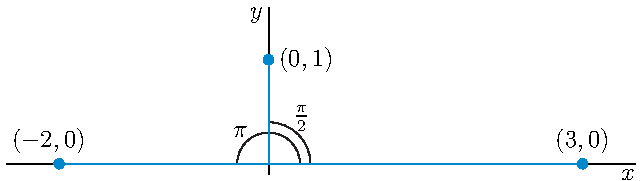
\includegraphics[scale=0.95]{polar3A.pdf}\quad
  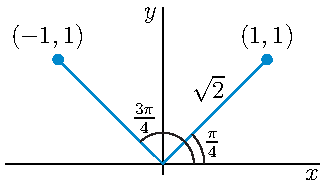
\includegraphics[scale=0.95]{polar2A.pdf}
\end{center}
    $r_1 = 3$,        $\theta_1=0$\qquad 
    $r_2 = \sqrt{2}$, $\theta_2=\frac{\pi}{4}$\qquad 
    $r_3 = 1$,        $\theta_3=\frac{\pi}{2}$\qquad 
    $r_4 = \sqrt{2}$, $\theta_4=\frac{3\pi}{4}$\\
    $r_5 = 2$,        $\theta_5=\pi$
\end{answer}


\begin{solution}
The left hand sketch below contains the points, $(x_1,y_1)$, $(x_3,y_3)$,
$(x_5,y_5)$, that are on the axes. The right hand sketch below contains the
points, $(x_2,y_2)$, $(x_4,y_4)$, that are not on the axes.
\begin{center}
  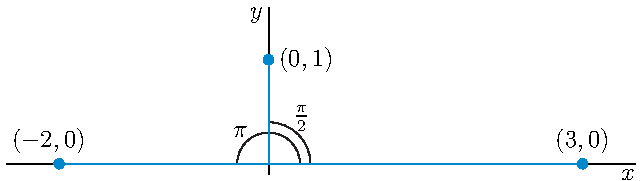
\includegraphics[scale=0.95]{polar3A.pdf}\quad
  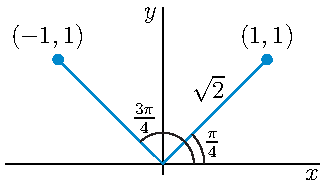
\includegraphics[scale=0.95]{polar2A.pdf}
\end{center}
Recall that the polar coordinates $r$, $\theta$
are related to the cartesian coordinates $x$, $y$, by $x=r\cos\theta$,
$y=r\sin\theta$. So $r=\sqrt{x^2+y^2}$ and $\tan\theta=\frac{y}{x}$
(assuming that $x\ne 0$) and
\begin{alignat*}{5}
(x_1,y_1) &= (3,0) &&\implies &r_1=3,\ \tan\theta_1=0
                   &&\implies \theta_1&=0 
                   \text{ as $(x_1,y_1)$ is on the positive $x$-axis} \\
(x_2,y_2) &= (1,1) &&\implies &r_2=\sqrt{2},\ \tan\theta_2=1
                   &&\implies \theta_2&=\frac{\pi}{4} 
                   \text{ as $(x_2,y_2)$ is in the first octant} \\
(x_3,y_3) &= (0,1) &&\implies &r_3=1,\ \cos\theta_3=0
                   &&\implies \theta_3&=\frac{\pi}{2} 
                   \text{ as $(x_3,y_3)$ is on the positive $y$-axis} \\
(x_4,y_4) &= (-1,1) &&\implies &r_4=\sqrt{2},\ \tan\theta_4=-1
                   &&\implies \theta_4&=\frac{3\pi}{4} 
                   \text{ as $(x_4,y_4)$ is in the third octant} \\
(x_5,y_5) &= (-2,0) &&\implies &r_5=2,\ \tan\theta_5=0
                   &&\implies \theta_5&=\pi 
                   \text{ as $(x_5,y_5)$ is on the negative $x$-axis} 
\end{alignat*}
\end{solution}


%%%%%%%%%%%%%%%%%%%%%%%%%%%
\begin{question}
\begin{enumerate}[(a)]
\item
Find \emph{all} pairs $(r,\theta)$ such that
\begin{equation*}
(-2,0) = \big(r\cos\theta\,,\,r\sin\theta\big)
\end{equation*}
\item
Find \emph{all} pairs $(r,\theta)$ such that
\begin{equation*}
(1,1) = \big(r\cos\theta\,,\,r\sin\theta\big)
\end{equation*}
\item
Find \emph{all} pairs $(r,\theta)$ such that
\begin{equation*}
(-1,-1) = \big(r\cos\theta\,,\,r\sin\theta\big)
\end{equation*}
\end{enumerate}
\end{question}

\begin{hint} 
$r$ is allowed to be negative.
\end{hint}

\begin{answer} 
(a) $\big(r=2\,,\,\theta= n\pi,\ n\text{ odd integer }\big)$ or 
    $\big(r=-2\,,\,\theta= n\pi,\ n\text{ even integer }\big)$ 

(b) $\big(r=\sqrt{2}\,,\,\theta= \nicefrac{\pi}{4} + 2n\pi\big)$ or 
    $\big(r=-\sqrt{2}\,,\,\theta= \nicefrac{5\pi}{4} + 2n\pi\big)$,
    with $n$ integer. 

(c) $\big(r=\sqrt{2}\,,\,\theta= \nicefrac{5\pi}{4} + 2n\pi\big)$ or 
    $\big(r=-\sqrt{2}\,,\,\theta= \nicefrac{\pi}{4} + 2n\pi\big)$,
    with $n$ integer. 
\end{answer}


\begin{solution}
Note that the distance from the point $\big(r\cos\theta\,,\,r\sin\theta\big)$
to the origin is
\begin{equation*}
\sqrt{r^2\cos^2\theta + r^2\sin^2\theta}
=\sqrt{r^2}
=|r|
\end{equation*}
Thus $r$ can be either the distance to the origin or minus the distance to the
origin.

(a) 
The distance from $(-2,0)$ to the origin is $2$. So either $r=2$ or $r=-2$.
\begin{itemize}
\item If $r=2$, then $\theta$ must obey 
\begin{align*}
(-2,0) = \big(2\cos\theta\,,\,2\sin\theta\big)
&\iff \sin\theta=0,\ \cos\theta=-1 \\
&\iff \theta= n\pi,\ n\text{ integer },\ \cos\theta=-1 \\
&\iff \theta= n\pi,\ n\text{ odd integer }
\end{align*}
\item If $r=-2$, then $\theta$ must obey 
\begin{align*}
(-2,0) = \big(-2\cos\theta\,,\,-2\sin\theta\big)
&\iff \sin\theta=0,\ \cos\theta=1 \\
&\iff \theta= n\pi,\ n\text{ integer },\ \cos\theta=1 \\
&\iff \theta= n\pi,\ n\text{ even integer }
\end{align*}
\end{itemize}
In the figure on the left below, the blue half-line is the set of all points 
with polar coordinates $\theta=\pi$, $r>0$ and the pink half-line is the set 
of all points  with polar coordinates $\theta=\pi$, $r<0$. 
In the figure on the right below, the blue half-line is the set of all points 
with polar coordinates $\theta=0$, $r>0$ and the pink half-line is the set 
of all points  with polar coordinates $\theta=0$, $r<0$. 
\begin{center}
  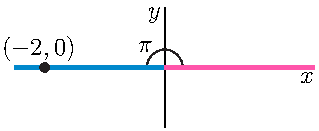
\includegraphics{polar6B.pdf}\qquad
  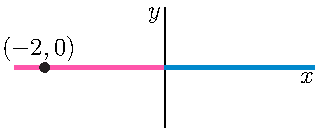
\includegraphics{polar6A.pdf}
\end{center}


(b)
The distance from $(1,1)$ to the origin is $\sqrt{2}$. 
So either $r=\sqrt{2}$ or $r=-\sqrt{2}$.
\begin{itemize}
\item If $r=\sqrt{2}$, then $\theta$ must obey 
\begin{align*}
(1,1) = \big(\sqrt{2}\,\cos\theta\,,\,\sqrt{2}\,\sin\theta\big)
&\iff \sin\theta=\cos\theta=\nicefrac{1}{\sqrt{2}} \\
&\iff \theta= \nicefrac{\pi}{4} + 2n\pi,\ n\text{ integer }
\end{align*}
\item If $r=-\sqrt{2}$, then $\theta$ must obey 
\begin{align*}
(1,1) = \big(-\sqrt{2}\,\cos\theta\,,\,-\sqrt{2}\,\sin\theta\big)
&\iff \sin\theta=\cos\theta=-\nicefrac{1}{\sqrt{2}} \\
&\iff \theta= \nicefrac{5\pi}{4} + 2n\pi,\ n\text{ integer }
\end{align*}
\end{itemize}
In the figure on the left below, the blue half-line is the set of all points 
with polar coordinates $\theta=\frac{\pi}{4}$, $r>0$ and the pink half-line 
is the set of all points  with polar coordinates $\theta=\frac{\pi}{4}$, $r<0$. 
In the figure on the right below, the blue half-line is the set of all points 
with polar coordinates $\theta=\frac{5\pi}{4}$, $r>0$ and the pink 
half-line is the set of all points  with polar coordinates 
$\theta=\frac{5\pi}{4}$, $r<0$. 
\begin{center}
  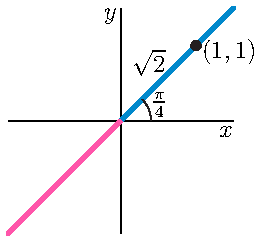
\includegraphics{polar4A.pdf}\qquad
  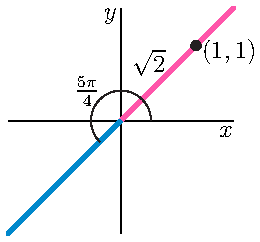
\includegraphics{polar4B.pdf}
\end{center}

(c)
The distance from $(-1,-1)$ to the origin is $\sqrt{2}$. 
So either $r=\sqrt{2}$ or $r=-\sqrt{2}$.
\begin{itemize}
\item If $r=\sqrt{2}$, then $\theta$ must obey 
\begin{align*}
(-1,-1) = \big(\sqrt{2}\,\cos\theta\,,\,\sqrt{2}\,\sin\theta\big)
&\iff \sin\theta=\cos\theta=-\nicefrac{1}{\sqrt{2}} \\
&\iff \theta= \nicefrac{5\pi}{4} + 2n\pi,\ n\text{ integer }
\end{align*}
\item If $r=-\sqrt{2}$, then $\theta$ must obey 
\begin{align*}
(-1,-1) = \big(-\sqrt{2}\,\cos\theta\,,\,-\sqrt{2}\,\sin\theta\big)
&\iff \sin\theta=\cos\theta=\nicefrac{1}{\sqrt{2}} \\
&\iff \theta= \nicefrac{\pi}{4} + 2n\pi,\ n\text{ integer }
\end{align*}
\end{itemize}
In the figure on the left below, the blue half-line is the set of all points 
with polar coordinates $\theta=\frac{5\pi}{4}$, $r>0$ and the pink half-line 
is the set of all points  with polar coordinates 
$\theta=\frac{5\pi}{4}$, $r<0$. 
In the figure on the right below, the blue half-line is the set of all points 
with polar coordinates $\theta=\frac{\pi}{4}$, $r>0$ and the pink 
half-line is the set of all points  with polar coordinates 
$\theta=\frac{\pi}{4}$, $r<0$. 
\begin{center}
  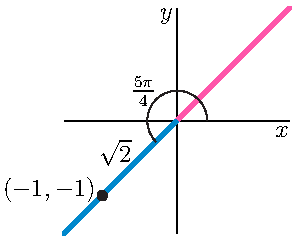
\includegraphics{polar5A.pdf}\qquad
  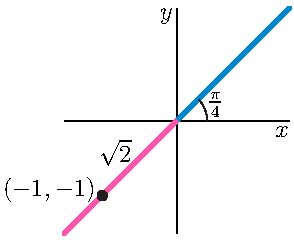
\includegraphics{polar5B.pdf}
\end{center}

\end{solution}



%%%%%%%%%%%%%%%%%%%%%%%%%%%
\begin{question}\label{prb polar vectors}
Consider the points
\begin{align*}
(x_1,y_1) &= (3,0) &
(x_2,y_2) &= (1,1)  &
(x_3,y_3) &= (0,1) \\
(x_4,y_4) &= (-1,1) &
(x_5,y_5) &= (-2,0)
\end{align*}
Also define, for each angle $\theta$, the vectors
\begin{align*}
\he_r(\theta)=\cos\theta\ \hi + \sin\theta\ \hj\qquad
\he_\theta(\theta) = -\sin\theta\ \hi + \cos\theta\ \hj
\end{align*}
\begin{enumerate}[(a)]
\item
Determine, for each angle $\theta$, the lengths of the vectors
$\he_r(\theta)$ and $\he_\theta(\theta)$ and the angle between 
the vectors $\he_r(\theta)$ and $\he_\theta(\theta)$. Compute
$\he_r(\theta)\times\he_\theta(\theta)$ (viewing $\he_r(\theta)$ and $\he_\theta(\theta)$ as vectors in three dimensions with zero $\hk$ 
components).
\item
For each $1\le i\le 5$, sketch, in the $xy$-plane, the point $(x_i,y_i)$
and the vectors $\he_r(\theta_i)$ and $\he_\theta(\theta_i)$. In your
sketch of the vectors, place the tails of the vectors 
$\he_r(\theta_i)$ and $\he_\theta(\theta_i)$ at $(x_i,y_i)$.
\end{enumerate}
\end{question}

\begin{hint} 
Compute, for each angle $\theta$, the dot product $\he_r(\theta)\cdot\he_\theta(\theta)$.
\end{hint}

\begin{answer} 
(a) Both $\he_r(\theta)$ and $\he_\theta(\theta)$ have length 1.
The angle between them is $\frac{\pi}{2}$. The cross product is
$\he_r(\theta) \times \he_\theta(\theta)=\hk$.

(b)
Here is a sketch of $(x_i,y_i)$, $\he_r(\theta_i)$,
$\he_\theta(\theta_i)$ for $i =1,3,5$ (the points on the axes)
\begin{center}
  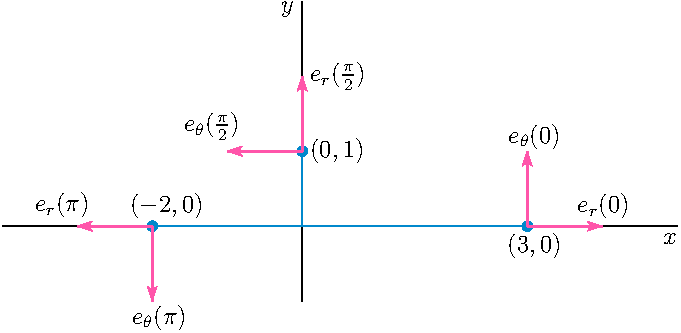
\includegraphics{polar3.pdf}
\end{center}
and here is a sketch (to a different scale) of $(x_i,y_i)$, $\he_r(\theta_i)$,
$\he_\theta(\theta_i)$ for $i =2,4$ (the points off the axes).
\begin{center}       
  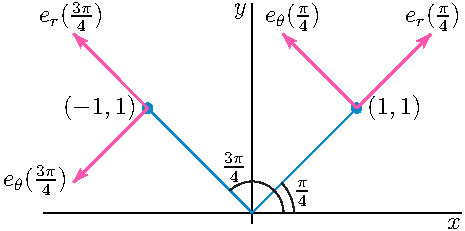
\includegraphics{polar2.pdf}
\end{center}
\end{answer}


\begin{solution} 
(a) The lengths are
\begin{align*}
|\he_r(\theta)| &= \sqrt{\cos^2\theta+\sin^2\theta} = 1 \\
|\he_\theta(\theta)| &= \sqrt{(-\sin\theta)^2+\cos^2\theta} = 1 
\end{align*}
As 
\begin{equation*}
\he_r(\theta) \cdot \he_\theta(\theta) = (\cos\theta)(-\sin\theta)
                                        +(\sin\theta)(\cos\theta)=0
\end{equation*}
the two vectors are perpendicular and the angle between them is 
$\frac{\pi}{2}$. The cross product is
\begin{align*}
\he_r(\theta) \times \he_\theta(\theta)
&=\det\left[\begin{matrix}
                  \hi  &  \hj        & \hk \\
           \cos\theta  & \sin\theta  &  0  \\
          -\sin\theta  & \cos\theta  &  0
            \end{matrix}\right] =\hk
\end{align*}

(b) Note that for $\theta$ determined by $x=r\cos\theta$, $y=r\sin\theta$,
\begin{itemize}\itemsep1pt \parskip0pt \parsep0pt %\itemindent-15pt
\item
the vector $\he_r(\theta)$ is a unit vector in the same direction as the
vector from $(0,0)$ to $(x,y)$ and 
\item
the vector $\he_\theta(\theta)$ is a unit vector that is perpendicular 
to $\he_r(\theta)$. 
\item
The $y$-component of $\he_\theta(\theta)$ has the same sign 
as the $x$-component of $\he_r(\theta)$.
The $x$-component of $\he_\theta(\theta)$ has opposite sign to that of the $y$-component  of $\he_r(\theta)$. 
\end{itemize}
Here is a sketch of $(x_i,y_i)$, $\he_r(\theta_i)$,
$\he_\theta(\theta_i)$ for $i =1,3,5$ (the points on the axes)
\begin{center}
  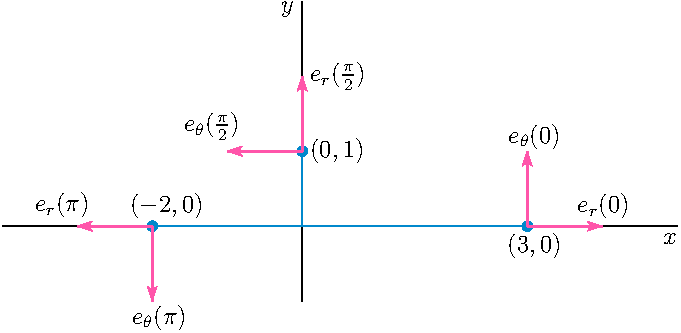
\includegraphics{polar3.pdf}
\end{center}
and here is a sketch (to a different scale) of $(x_i,y_i)$, $\he_r(\theta_i)$,
$\he_\theta(\theta_i)$ for $i =2,4$ (the points off the axes).
\begin{center}       
  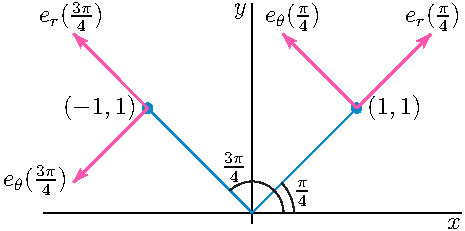
\includegraphics{polar2.pdf}
\end{center}
\end{solution}

%%%%%%%%%%%%%%%%%%%%%%%%%%%%%%%%
\begin{question}[M200 2008A] %7
Match the following equations with the corresponding 
pictures. Cartesian coordinates are $(x, y)$ and polar coordinates are 
$(r, \theta)$.

\begin{center}
 (A) \raisebox{-0.5\height}
           {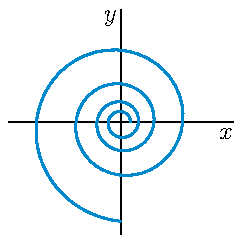
\includegraphics[width=0.33\textwidth, height=0.3\textwidth]
                                                   {polarCurveE.pdf}}
\qquad
  (B) \raisebox{-0.5\height}
            {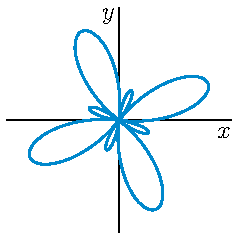
\includegraphics[width=0.33\textwidth, height=0.33\textwidth]
                                                   {polarCurveB.pdf}}
\end{center}
\begin{center}
  (C) \raisebox{-0.5\height}
            {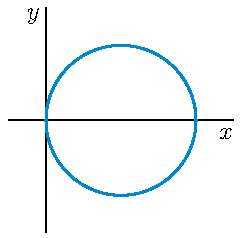
\includegraphics[width=0.33\textwidth, height=0.33\textwidth]
                                                   {polarCurveC.pdf}}
\qquad
  (D)  \raisebox{-0.5\height} 
            { 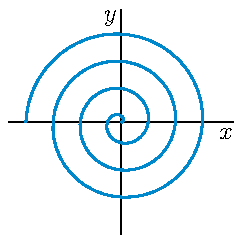
\includegraphics[width=0.33\textwidth, height=0.3\textwidth]
                                                    {polarCurveF.pdf}}
\end{center}
\begin{center}
 (E) \raisebox{-0.5\height}
           { 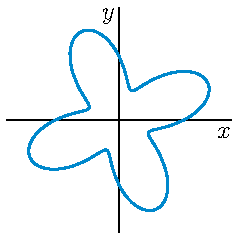
\includegraphics[width=0.33\textwidth, height=0.3\textwidth]
                                                    {polarCurveA.pdf}}
\qquad
  (F) \raisebox{-0.5\height}
           {  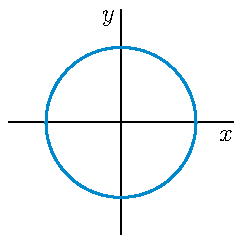
\includegraphics[width=0.33\textwidth, height=0.3\textwidth]
                                                    {polarCurveD.pdf}}
\end{center}

\begin{alignat*}{7}
&\text{(a)}\quad& r&=2+\sin(4\theta) \qquad\qquad &
&\text{(b)}\quad& r&=1+2\sin(4\theta)\qquad\qquad &
&\text{(c)}\quad& r&=1\\
&\text{(d)}& r&=2\cos(\theta),\ 
           -\tfrac{\pi}{2}\le\theta\le\tfrac{\pi}{2}\qquad\qquad &
&\text{(e)}& r&=e^{\theta/10}+e^{-\theta/10}\qquad\qquad &
&\text{(f)}& r&=\theta &
\end{alignat*}
\end{question}

%\begin{hint}
%
%\end{hint}

\begin{answer}
(a) $\leftrightarrow$ (E) \qquad
(b) $\leftrightarrow$ (B) \qquad
(c) $\leftrightarrow$ (F) \qquad
(d) $\leftrightarrow$ (C) \qquad
(e) $\leftrightarrow$ (A) \qquad
(f) $\leftrightarrow$ (D)
\end{answer}

\begin{solution}
(a) Since $-1\le \sin(4\theta)\le 1$, the coordinate $r=2+\sin(4\theta)$ oscillates between $r=1$ and $r=3$ as $\theta$ runs from $0$ to $2\pi$.
The maximum value $r=3$ is achieved when $\sin(4\theta)=1$, i.e when
$4\theta=\frac{\pi}{2} +2n\pi$, i.e. when $\theta=\frac{\pi}{8}+\frac{n\pi}{2}$.
That matches figure (E).

(b) Since $-1\le \sin(4\theta)\le 1$, the coordinate $r=1+2\sin(4\theta)$ takes its maximum value $r=3$ when $\sin(4\theta)=1$, i.e. when $\theta=\frac{\pi}{8}+\frac{n\pi}{2}$, just as the case with $(a)$. But now
$r$ can also take the value $0$. That matches figure (B).

(c) $r=1$ is completely indepedent of $\theta$. All points on the curve $r=1$
are a distance $1$ from the origin. That is, $r=1$ is the circle of radius $1$
centred on the origin. That's figure (F).

(d) In this case, $\theta$ is subject to the restriction 
$-\frac{\pi}{2}\le\theta\le\frac{\pi}{2}$, like figure (C).
Figure (C) looks like a circle. We can verify that $r=2\cos(\theta)$ is 
indeed a circle by converting to Cartesian coordinates. We can convert the right hand side to exactly $2x=2r\cos(\theta)$ by multiplying the 
whole equation by $r$.
\begin{align*}
r=2\cos(\theta)
&\iff r^2 =2r\cos(\theta)
\iff x^2+y^2=2x \\
&\iff (x-1)^2+y^2=1
\end{align*}
So $r=2\cos(\theta)$ is the circle of radius $1$ centred on $x=1$, $y=0$,
which indeed matches figure (C).

(e) When $\theta=0$, $r=e^{\theta/10}+e^{-\theta/10}=2$.
As 
\begin{equation*}
\diff{}{\theta}\big(e^{\theta/10}+e^{-\theta/10}\big)
    =\frac{1}{10}\big(e^{\theta/10}-e^{-\theta/10}\big)
    >0\qquad\text{for all }\theta > 0
\end{equation*}
$r=e^{\theta/10}+e^{-\theta/10}$ increases as $\theta$ increases for all
$\theta\ge 0$. Furthermore the rate of increase gets bigger and bigger as 
$\theta$ gets bigger and bigger. So $r$ starts at $r=2$ when $\theta=0$
and increases faster and faster as $\theta$ increases. That matches figure (A).

(f) When $\theta=0$, $r=\theta=0$.
As 
\begin{equation*}
\diff{}{\theta} \theta
    =1 \qquad\text{for all }\theta
\end{equation*}
$r=\theta$ increases as $\theta$ increases for all
$\theta\ge 0$. Furthermore the rate of increase is independent of $\theta$.
So $r$ starts at $r=0$ when $\theta=0$
and increases at a constant rate as $\theta$ increases.
That matches figure (D).

\end{solution}


%%%%%%%%%%%%%%%%%%
\subsection*{\Procedural}
%%%%%%%%%%%%%%%%%%

%%%%%%%%%%%%%%%%%%%%%%%%%%%
\begin{question}\label{prb polar curvature}
Recall that a point with polar coordinates $r$ and
$\theta$ has $x=r\cos\theta$ and $y=r\sin\theta$. Let $r=f(\theta)$ be 
the equation of a plane curve in polar coordinates. Find the 
curvature of this curve at a general point $\theta$. 
\end{question}

\begin{hint} 
The curve can be parametrized by 
$\vr(\theta)= f(\theta)\big[\cos\theta\ \hi + \sin\theta\ \hj\big]$
\end{hint}

\begin{answer} 
$\ka(\theta)=\frac{\big|f(\theta)^2+2f'(\theta)^2-f(\theta)f''(\theta)\big|}
                     {{[f(\theta)^2+f'(\theta)^2]}^{3/2}}$
\end{answer}


\begin{solution}
Think of $\theta$ as a time parameter and recall that
$\ka(\theta)=\frac{|\vv(\theta)\times\va(\theta)|}{|\vv(\theta)|^3}$.
The given curve has
\begin{align*}
x(\theta)&= f(\theta)\cos\theta\\
y(\theta)&= f(\theta)\sin\theta \\
\vr(\theta)&= f(\theta)\big[\cos\theta\ \hi + \sin\theta\ \hj\big] \\
\vv(\theta)=\vr'(\theta)&= f'(\theta)\big[\cos\theta\ \hi + \sin\theta\ \hj\big]
          +f(\theta)\big[-\sin\theta\ \hi + \cos\theta\ \hj\big] \\
\va(\theta)=\vr''(\theta)&= \big\{f''(\theta)-f(\theta)\big\}\big[\cos\theta\ \hi + \sin\theta\ \hj\big]
             +2f'(\theta)\big[-\sin\theta\ \hi + \cos\theta\ \hj\big]  
\end{align*}
The efficient way to compute $|\vv(\theta)|$ and
the cross product $\vv(\theta)\times\va(\theta)$
is to observe that
\begin{align*}
\vv(\theta)&= f'(\theta)\,\he_r(\theta) +f(\theta)\,\he_\theta(\theta) \\
\va(\theta)&= \big\{f''(\theta)-f(\theta)\big\}\,\he_r(\theta)
             +2f'(\theta)\,\he_\theta(\theta)
\end{align*}
where $\he_r(\theta)$ and $\he_\theta(\theta)$ are the vectors of
Q[\ref{prb polar vectors}].  As $\he_r(\theta)$ and $\he_\theta(\theta)$
are mutually perpendicular unit vectors
obeying $\he_r(\theta)\times\he_\theta(\theta) =\hk$ and 
$\he_r(\theta)\times\he_r(\theta) = \he_\theta(\theta)\times\he_\theta(\theta) =0$,
\begin{align*}
|\vv(\theta)|^2=\vv(\theta)\cdot\vv(\theta)
   &=\big[f'(\theta)\,\he_r(\theta) +f(\theta)\,\he_\theta(\theta)\big]\cdot
     \big[f'(\theta)\,\he_r(\theta) +f(\theta)\,\he_\theta(\theta)\big] \\
   &=f'(\theta)^2\,\he_r(\theta)\cdot\he_r(\theta)
     +f(\theta)^2\,\he_\theta(\theta)\cdot\he_\theta(\theta)
     +2f'(\theta)\,f(\theta)\,\he_r(\theta)\cdot\he_\theta(\theta) \\
   &=f'(\theta)^2+f(\theta)^2  \\
|\vv(\theta)|& = \sqrt{f'(\theta)^2+f(\theta)^2}\\
\vv(\theta)\times\va(\theta) 
 &=\big[f'(\theta)\,\he_r(\theta) +f(\theta)\,\he_\theta(\theta)\big]\times
   \big[\big\{f''(\theta)-f(\theta)\big\}\,\he_r(\theta)
             +2f'(\theta)\,\he_\theta(\theta)\big] \\
 &= 2f'(\theta)^2\,\he_r(\theta)\times\he_\theta(\theta)
  +f(\theta)[f''(\theta)-f(\theta)]\,\he_\theta(\theta)\times\he_r(\theta)
                                \\
 &= \big\{2f'(\theta)^2-f(\theta)[f''(\theta)-f(\theta)]\big\}
                                \,\hk
\end{align*}
So
\begin{align*}
\ka(\theta)&=\frac{|\vv(\theta)\times\va(\theta)|}{|\vv(\theta)|^3}
=\frac{\big|f(\theta)^2+2f'(\theta)^2-f(\theta)f''(\theta)\big|}
                     {{[f(\theta)^2+f'(\theta)^2]}^{3/2}}
\end{align*}
\end{solution}



%%%%%%%%%%%%%%%%%%%%%%%%%%%
\begin{question}
Find the curvature of the cardioid $r=a(1-\cos\theta)$.
\end{question}

%\begin{hint} 
%\end{hint}

\begin{answer} 
$\ka(\theta)=\frac{3}{2^{3/2}a\sqrt{1-\cos\theta}}
   =\frac{3}{2\sqrt{2ar(\theta)}}$
\end{answer}


\begin{solution}
By the Q[\ref{prb polar curvature}] with
\begin{align*}
f(\theta)  = a(1-\cos\theta)\qquad
f'(\theta) = a\sin\theta\qquad
f''(\theta) =a\cos\theta
\end{align*}
we have
\begin{align*}
\ka(\theta)
&=\frac{\big|f(\theta)^2+2f'(\theta)^2-f(\theta)f''(\theta)\big|}
                     {[f(\theta)^2+f'(\theta)^2]^{3/2}}\\
&=\frac{\big|a^2-2a^2\cos\theta+a^2\cos^2\theta+2a^2\sin^2\theta-
                a^2\cos\theta+a^2\cos^2\theta\big|}
        {[a^2-2a^2\cos\theta+a^2\cos^2\theta+a^2\sin^2\theta]^{3/2}}\\
&=\frac{3a^2-3a^2\cos\theta}{[2a^2-2a^2\cos\theta]^{3/2}}
=\frac{3}{2^{3/2}a\sqrt{1-\cos\theta}}
=\frac{3}{2\sqrt{2ar(\theta)}}
\end{align*}
\end{solution}

%%%%%%%%%%%%%%%%%%
%\subsection*{\Application}
%%%%%%%%%%%%%%%%%%









%\section{Central Forces}
%%\documentclass[12pt]{article}

\questionheader{ex:s1.9}

%%%%%%%%%%%%%%%%%%
%\subsection*{\Conceptual}
%%%%%%%%%%%%%%%%%%


%%%%%%%%%%%%%%%%%%
\subsection*{\Procedural}
%%%%%%%%%%%%%%%%%%

%%%%%%%%%%%%%%%%%%
\subsection*{\Application}
%%%%%%%%%%%%%%%%%%


%%%%%%%%%%%%%%%%%%%%%%%%%%%
\begin{question}[M317 2010A] %3
Let $\vr(t) = x(t)\,\hi + y (t)\,\hj + z(t)\,\hk$ be the position 
of a particle at time $t$ . Suppose the motion of the particle satisfies 
the differential equation
$\difftwo{\vr}{t} = f (r) \vr$ 
where $r = |\vr|$ .
\begin{enumerate}[(a)]
\item
Suppose $f(r)$ is an arbitrary function of $r$ . Prove or disprove each 
of the following statements.
\begin{enumerate}[(i)]
\item
The motion of the particle is planar.
\item
The path of the particle sweeps out equal areas in equal times.
\end{enumerate}
\item
Find all forms of $f(r)$ for which the motion of the particle always lies 
on a straight line.
\item
Give a specific form of $f(r)$ for which the motion of the particle could 
lie on an ellipse.
\end{enumerate}
\end{question}

\begin{hint} 
(a) Review \S\eref{CLP317}{sec:central forces} of the CLP-4 text.

(b) Any straight line can be parametrized as $\vr(s) = \vr_0+\hat\vT\, s$.

(c) Review \S\eref{CLP317}{sec:planet} of the CLP-4 text.
\end{hint}

\begin{answer}
(a) See the solutions. 

(b) $f(r)=0$ for all $r\ge 0$.

(c) Any $f(r)$ which is a positive constant times $-\frac{1}{r^3}$ works.
\end{answer}

\begin{solution} (a)
Both (i) and (ii) were proven in \S\eref{CLP317}{sec:central forces} 
of the CLP-4 text. Here are those arguments.

Define
\begin{equation*}
\vOm(t) = \vr(t)\times\vv(t)
\end{equation*}
By the product rule,
\begin{equation*}
\diff{\vOm}{t}(t) =\diff{\ }{t}\big(\vr(t)\times\vv(t)\big)
=\vv(t)\times\vv(t) + \vr(t)\times\va(t)
=m\vr(t)\times f\big(r(t))\vr(t)\big)
=\vZero
\end{equation*}
So $\vOm(t)$ is in fact independent of $t$. It is a constant vector that
we'll just denote $\vOm$. 

As $\vr(t)\times\vv(t)=\vOm$, we have that
$\vr(t)$ is always perpendicular to $\vOm$ and
\begin{equation*}
\vr(t)\cdot\vOm =0
\end{equation*}
\begin{itemize}\itemsep1pt \parskip0pt \parsep0pt %\itemindent-15pt
\item[$\circ$]
If $\vOm\ne \vZero$, this is exactly the statement that $\vr(t)$ always 
lies in the plane through the origin with normal vector $\vOm$.
\item[$\circ$]
If $\vOm=\vZero$, then $\vr(t)$ is always parallel to $\vv(t)$ and there
is some function $\alpha(t)$ such that
\begin{equation*}
\diff{\vr}{t}(t) = \vv(t) = \alpha(t)\,\vr(t)
\end{equation*}
This is a first order, linear, ordinary differential equation that we can solve
by using an integrating factor. Set
\begin{equation*}
\beta(t) = \int_0^t\alpha(t)\ \dee{t}
\end{equation*}
Then
\begin{align*}
\diff{\vr}{t}(t) = \alpha(t)\,\vr(t)
&\iff e^{-\beta(t)} \diff{\vr}{t}(t) -\alpha(t)e^{-\beta(t)}\,\vr(t)=0\\
&\iff \diff{\ }{t}\big[e^{-\beta(t)}\vr(t)\big] = 0\\
&\iff e^{-\beta(t)}\vr(t) = \vr(0)\\
&\iff \vr(t) =  e^{\beta(t)}\vr(0)
\end{align*}
so that $\vr(t)$ lies on a line through the origin. This makes sense ---
the particle is always moving parallel to its radius vector.
\end{itemize}
This completes the verification that $\vr(t)$ lies in a plane.

Now we show that the radius vector $\vr(t)$ sweeps out equal areas in 
equal times. In other words, we now verify that the rate at which 
$\vr(t)$ sweeps out area is independent of time. To do so we rewrite the
statement that $|\vr(t)\times\vv(t)\big|$ is constant in polar coordinates.
Writing $\vr(t) = r(t)\hat\vr\big(\theta(t)\big)$ and then applying
Lemma \eref{CLP317}{lem:polar}.b of the CLP-4 text gives that
\begin{align*}
\text{constant} = \big|\vr\times\vv\big| 
   = \Big|r\hat\vr\times\Big(\diff{r}{t}\ \hat\vr 
             + r\ \diff{\theta}{t}\ \hat\vth\Big)\Big|
   =r^2\diff{\theta}{t}
\qquad\text{since}\quad |\hat\vr\times\hat\vr|=0,\ 
                        |\hat\vr\times\hat\vth|=1
\end{align*}
is constant. It now suffices to observe that $r(t)^2\diff{\theta}{t}(t)$ 
is exactly twice the rate at which $\vr(t)$ sweeps out area. To see this,
just look at the figure below. The shaded area is essentially a wedge of
a circular disk of radius $r$. (If $r(t)$ were independent of $t$, it would be exactly a wedge of a circular disk.) Its area is the 
fraction $\frac{\dee{\theta}}{2\pi}$ of the area of the full disk, which is
\begin{equation*}
\frac{\dee{\theta}}{2\pi}\ \pi r^2 = \frac{1}{2}r^2\,\dee{\theta}
\qquad\qquad\raisebox{-0.35\height}[42pt][20pt]{
                 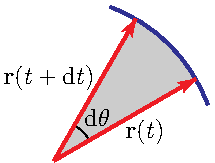
\includegraphics{equalArea.pdf}}
\end{equation*}

\noindent (b) If $f(r)$ is identically zero, then $\vr''(t)=0$,
so that $\vr'(t)$ is a constant, say $\vv_0$, and $\vr(t) = \vr_0 + \vv_0 t$,
for some constant $\vr_0$. That's a straight line.

We'll now show that if the motion of the particle always lies 
on a straight line, then $f(r)$ must be identically zero.
Suppose that $\vr(t)$ is a straight line. Then there are 
constant vectors $\vr_0$ and $\hat\vT$ such that $\vr(t) =\vr_0+ g(t)\hat\vT$
for some scalar valued function $g(t)$. Then
\begin{align*}
\vr''(t) &= f\big(r(t)\big)\vr(t) \\
\end{align*}
becomes
\begin{align*}
g''(t)\hat\vT & = f\big(r(t)\big)\,\big[\vr_0+ g(t)\hat\vT\big]
              = f\big(r(t)\big)\,\vr_0
               + f\big(r(t)\big) g(t)\hat\vT
\end{align*}
We may always choose the initial conditions so that, for example, 
$\vr_0=\hi$ and $\hat\vT=\hj$.  So
\begin{align*}
g''(t)\hj &   = f\big(r(t)\big)\,\hi
               + f\big(r(t)\big) g(t)\hj
\end{align*}
Taking the dot product of both sides with $\hi$ gives 
$f\big(r(t)\big)=0$, as desired.


\noindent (c) We saw in \S\eref{CLP317}{sec:planet} of the CLP-4 text
that the gravitational force $-\frac{GMm}{r^3}\vr$ can produce 
elliptical orbits.
So any $f(r)$ which is a positive constant times $-\frac{1}{r^3}$ does 
the job. 

\end{solution}


%%%%%%%%%%%%%%%%%%%%%%%%%%%
\begin{question}[M317 2000A] %6
An object moves along a curve in the $xy$-plane having polar
equation $r=\frac{1}{\theta+\al}$ (where $\al$ is a constant) under the influence
of a central force so that the object has no transverse acceleration.
\begin{enumerate}[(a)]
\item
Verify that $r^2\dot\theta=h$ remains constant as the object
moves.
\item
Express the magnitude of the acceleration of the object as
a function of $r$ and $h$.
\end{enumerate}

\end{question}

\begin{hint} 
(a) For any central force $\big|\vr(t)\times\vv(t)\big|$ is independent of $t$.

(b) Review Lemma \eref{CLP317}{lem:polar} in the CLP-4 text.
\end{hint}

\begin{answer}
(a) See the solution.

(b) $|\va(t)| =\frac{h^2}{r(t)^3}$
\end{answer}

\begin{solution} 
(a)
Our object is subject to a central force. So the acceleration $\va(t)$
is parallel to $\vr(t)$ and
\begin{equation*}
\diff{\ }{t}\big(\vr(t)\times\vv(t)\big)
=\vv(t)\times\vv(t) + \vr(t)\times\va(t)
=\vZero +\vZero
=\vZero
\end{equation*}
By Lemma \eref{CLP317}{lem:polar} of the CLP-4 text,
$\vv(t) = \diff{r}{t}(t)\ \hat\vr\big(\theta(t)\big) 
             + r(t)\ \diff{\theta}{t}(t)\ \hat\vth\big(\theta(t)\big)$.
Because $\vr(t)=r(t)\hat\vr\big(\theta(t)\big)$ is parallel to 
$\hat\vr\big(\theta(t)\big)$ and is perpendicular to 
$\hat\vth\big(\theta(t)\big)$,
\begin{equation*}
\vr(t)\times\vv(t)
=r(t)^2\dot\theta(t)\,\hat\vr\big(\theta(t)\big)\times
                       \hat\vth\big(\theta(t)\big)
\end{equation*}
and, in particular,
\begin{equation*}
|\vr(t)\times\vv(t)| = r(t)^2|\dot\theta(t)|
\end{equation*}
is a constant. As $\dot\theta(t)$ is continuous, $r(t)^2\dot\theta(t)$
is also constant.

(b) 
By Lemma \eref{CLP317}{lem:polar} of the CLP-4 text,
the acceleration
\begin{equation*}
\va(t) = \Big(\difftwo{r}{t}(t)-r(t)\Big(\diff{\theta}{t}(t)\Big)^2\Big) 
             \hat\vr\big(\theta(t)\big)
   +\Big(r(t)\ \difftwo{\theta}{t}(t) 
          + 2 \diff{r}{t}(t)\diff{\theta}{t}(t)\Big)
                  \hat\vth\big(\theta(t)\big)
\end{equation*}
Because our object is subject to a central force, the acceleration 
$\va(t)$ is parallel to $\hat\vr\big(\theta(t)\big)$. So the 
$\hat\vth\big(\theta(t)\big)$ component of the acceleration is zero 
and
\begin{equation*}
\va(t) = \Big(\difftwo{r}{t}(t)-r(t)\Big(\diff{\theta}{t}(t)\Big)^2\Big) 
             \hat\vr\big(\theta(t)\big)
\end{equation*}
so that
\begin{equation*}
|\va(t)| = \Big|\difftwo{r}{t}(t)-r(t)\Big(\diff{\theta}{t}(t)\Big)^2\Big|
\end{equation*}
Since $r(t)=\frac{1}{\theta(t)+\al}$
\begin{align*}
\dot r(t) = - \frac{1}{[\theta(t)+\al]^2}\dot\theta(t)
          =- r(t)^2 \dot\theta(t) =-h
\end{align*}
So $\difftwo{r}{t}(t)=0$ and
\begin{align*}
|\va(t)| = r(t)\dot\theta(t)^2
=\frac{r(t)^4\dot\theta(t)^2}{r(t)^3}
=\frac{h^2}{r(t)^3}
\end{align*}

\end{solution}








%%%%%%%%%%%%%%%%%%%%%%%%%%%%%%%%%%%%%
\chapter{Vector Fields}
\section{Definitions and First Examples}
%\documentclass[12pt]{article}

\questionheader{ex:s2.1}

%%%%%%%%%%%%%%%%%%
\subsection*{\Conceptual}
%%%%%%%%%%%%%%%%%%

%%%%%%%%%%%%%%%%%%
\begin{question}
Below is a sketch of the vector field $\vv(x,y)$. 

\[
\begin{tikzpicture}%\vv(x,y)=(x, (sinx)/(y^2+2)), -pi < x < pi
\YEaxis{5.5}{3.5}
\foreach \x in {-1,-2,-3,-4,1,2,3,4}{
\YExcoord{\x}{}
}
\foreach \x in {-1,-2,-3,1,2,3}{
\YEycoord{\x}{}
}
\foreach \x in {-4,...,4}{
\foreach \y in {-3,...,3}{
\MULTIPLY{\x}{\numberPI}{\xpi}
\DIVIDE{\xpi}{4}{\xx}
\COS{\xx}{\cosx}
\POWER{\y}{2}{\ysq}
\ADD{\ysq}{2}{\denom}
\DIVIDE{\cosx}{\denom}{\ynew}
\DIVIDE{\x}{4}{\xnew}%scale
	\draw[->, red, thick] (\x,\y)--({\x+\xnew},{\y+\ynew});
	}}
\end{tikzpicture}
\]

Find the regions where the $x$-coordinates and $y$-coordinates are positive, negative, and zero:
$\vv(x,y)\cdot \hi \begin{cases}
>0 & \mbox{ when } \fbox{\vphantom{L}\hspace{2cm}}\\
=0 &\mbox{ when } \fbox{\vphantom{L}\hspace{2cm}}\\
<0&\mbox{ when } \fbox{\vphantom{L}\hspace{2cm}}
\end{cases}$\qquad
$\vv(x,y)\cdot \hj \begin{cases}
>0 & \mbox{ when } \fbox{\vphantom{L}\hspace{2cm}}\\
=0 &\mbox{ when } \fbox{\vphantom{L}\hspace{2cm}}\\
<0&\mbox{ when } \fbox{\vphantom{L}\hspace{2cm}}
\end{cases}$

You may assume that $\vv(x,y)$ behaves as expected at the points you don't see. That is, the samples are representative of a smooth, continuous vector-valued function. You may also assume the tick marks on the axes correspond to unit distances.
\end{question}

\begin{hint} 
Not all blanks represent a single interval.
\end{hint}

\begin{answer} 
$\vv(x,y)\cdot \hi \left.\begin{cases}
>0 & \mbox{ when } \fbox{$x>0$}\\
=0 &\mbox{ when } \fbox{$x=0$}\\
<0&\mbox{ when } \fbox{$x<0$}
\end{cases}\right\}$
and
$\vv(x,y)\cdot \hj \left.\begin{cases}
>0 & \mbox{ when } \fbox{$-2<x<2$}\\
=0 &\mbox{ when } \fbox{$x \in \{-2,2\}$}\\
<0&\mbox{ when } \fbox{$x<-2$ or $x>2$}
\end{cases}\right\}$\quad
at least for $(x,y)$ shown in the sketch.
\end{answer}

\begin{solution}
The vectors are pointing to the right when $x>0$, to the left when $x<0$, and are vertical when $x=0$. So, at least for $(x,y)$ shown in the sketch,
\[\vv(x,y)\cdot \hi \begin{cases}
>0 & \mbox{ when } \fbox{$x>0$}\\
=0 &\mbox{ when } \fbox{$x=0$}\\
<0&\mbox{ when } \fbox{$x<0$}
\end{cases}\]
The behaviour of the $y$-values is more complicated. Vectors in one vertical line seem to be all pointing up, or all pointing down. So, the sign of $\vv\cdot\hj$ depends only on $x$, not on $y$ (although the \emph{magnitude} of $\vv\cdot\hj$ depends on both). Roughly,  the vectors are pointing
\begin{itemize}
\item Down when $x<-2$;
\item horizontally when $x=-2$ (remember the vector is positioned with the \emph{base} of $\vv(x,y)$ at $(x,y)$;
\item up when $-2<x<2$;
\item horizontally  when $x=2$;
\item up when $2<x$.
\end{itemize}

Since we're assuming there's nothing surprising happening between the samples pictured, at least for $(x,y)$ shown in the sketch,

\[\vv(x,y)\cdot \hj \begin{cases}
>0 & \mbox{ when } \fbox{$-2<x<2$}\\
=0 &\mbox{ when } \fbox{$x \in \{-2,2\}$}\\
<0&\mbox{ when } \fbox{$x<-2$ or $x>2$}
\end{cases}\]

\end{solution}
%%%%%%%%%%%%%%%%%%%%%%%%%%%%%%%%%%%%
\begin{question}
Below is a sketch of the vector field $\vv(x,y)$. 

\[
\begin{tikzpicture}[xscale=1.2] %\vv(x,y)=(x+y,x-y)
\YEaxis{5.5}{5.5}
\foreach \x in {-1,-2,-3,-4,1,2,3,4}{
\YExcoord{\x}{}
\YEycoord{\x}{}
}
\foreach \x in {-4,...,4}{
\foreach \y in {-4,...,4}{
\ADD{\x}{\y}{\xnew}
\SUBTRACT{\x}{\y}{\ynew}
\POWER{\x}{2}{\xtest}
\POWER{\y}{2}{\ytest}
\ADD{\xtest}{\ytest}{\test}
	\ifnum \test = 0
		{}
		\else
		\draw[->, red, thick] (\x,\y)--({\x+\xnew/6},{\y+\ynew/6});
	\fi
	}}
\draw[dotted]  (-4,-4) grid (4,4);
\end{tikzpicture}
\]

Find the regions where the $x$-coordinates and $y$-coordinates are positive, negative, and zero:

$\vv(x,y)\cdot \hi \begin{cases}
>0 & \mbox{ when } \fbox{\vphantom{L}\hspace{2cm}}\\
=0 &\mbox{ when } \fbox{\vphantom{L}\hspace{2cm}}\\
<0&\mbox{ when } \fbox{\vphantom{L}\hspace{2cm}}
\end{cases}$\qquad
$\vv(x,y)\cdot \hj \begin{cases}
>0 & \mbox{ when } \fbox{\vphantom{L}\hspace{2cm}}\\
=0 &\mbox{ when } \fbox{\vphantom{L}\hspace{2cm}}\\
<0&\mbox{ when } \fbox{\vphantom{L}\hspace{2cm}}
\end{cases}$

You may assume that the samples shown are representative of the general behaviour of $\vv(x,y)$. You may also assume the tick marks on the axes correspond to unit distances.
\end{question}

\begin{hint} 
Write down all coordinates where $\vv(x,y)\cdot\hi=0$ or $\vv(x,y)\cdot\hj=0$, and look for a pattern.
\end{hint}

\begin{answer} 
$\vv(x,y)\cdot \hi \left.\begin{cases}
>0 & \mbox{ when } \fbox{$y>-x$}\\
=0 &\mbox{ when } \fbox{$y=-x$}\\
<0&\mbox{ when } \fbox{$y<-x$}
\end{cases}\right\}$ \quad and\quad
$\vv(x,y)\cdot \hj \left.\begin{cases}
>0 & \mbox{ when } \fbox{$y<x$}\\
=0 &\mbox{ when } \fbox{$y=x$}\\
<0&\mbox{ when } \fbox{$y>x$}
\end{cases}\right\}$\quad
at least for $(x,y)$ shown in the sketch.
\end{answer}

\begin{solution}
To start out, we find the places where $\vv(x,y)\cdot\hi=0$ (vertical vectors) or $\vv(x,y)\cdot\hj=0$ (horizontal vectors). Remember the vector $\vv(x,y)$ has its \emph{tail} at $(x,y)$.

We see the vertical vectors  (those with $\vv(x,y)\cdot\hi=0$) occur at every point along the line $y=-x$, while 
horizontal vectors  (those with $\vv(x,y)\cdot\hj=0$) occur at every point along the line $y=x$.



Indeed, below the line $y=-x$, vectors point to the left, while above the line $y=-x$ they point to the right.
Similarly, vectors point down when they're above the line $y=x$, and the point up when they're below the line $y=x$.

\begin{tikzpicture}[scale=0.6] %\vv(x,y)=(x+y,x-y)
\fill[blue, opacity=0.3] (-5,5)|-(5,-5);
\draw[blue, dashed] (-5,5)--(5.5,-5.5);
\draw[blue] (-2.5,-6) node{LEFT};
\draw[red] (2.5,5.5) node{RIGHT};
\YEaxis{5.5}{5.5}
\foreach \x in {-1,-2,-3,-4,1,2,3,4}{
\YExcoord{\x}{}
\YEycoord{\x}{}
}
\foreach \x in {-4,...,4}{
\foreach \y in {-4,...,4}{
\ADD{\x}{\y}{\xnew}
\SUBTRACT{\x}{\y}{\ynew}
\POWER{\x}{2}{\xtest}
\POWER{\y}{2}{\ytest}
\ADD{\xtest}{\ytest}{\test}
	\ifnum \test = 0
		{}
		\else
		\draw[->, red, thick] (\x,\y)--({\x+\xnew/6},{\y+\ynew/6});
	\fi
	}}
\draw[dotted]  (-4,-4) grid (4,4);
\end{tikzpicture}\hfill
\begin{tikzpicture}[scale=0.6] %\vv(x,y)=(x+y,x-y)
\fill[blue, opacity=0.3] (-5,-5)-|(5,5);
\draw[blue,dashed] (-5,-5)--(5.5,5.5) ;
\draw[blue] (2.5,-6) node{UP};
\draw[red] (-2.5,5.5) node{DOWN};
\YEaxis{5.5}{5.5}
\foreach \x in {-1,-2,-3,-4,1,2,3,4}{
\YExcoord{\x}{}
\YEycoord{\x}{}
}
\foreach \x in {-4,...,4}{
\foreach \y in {-4,...,4}{
\ADD{\x}{\y}{\xnew}
\SUBTRACT{\x}{\y}{\ynew}
\POWER{\x}{2}{\xtest}
\POWER{\y}{2}{\ytest}
\ADD{\xtest}{\ytest}{\test}
	\ifnum \test = 0
		{}
		\else
		\draw[->, red, thick] (\x,\y)--({\x+\xnew/6},{\y+\ynew/6});
	\fi
	}}
\draw[dotted]  (-4,-4) grid (4,4);
\end{tikzpicture}



So, at least for $(x,y)$ shown in the sketch,
\begin{equation*}
\vv(x,y)\cdot \hi \begin{cases}
>0 & \mbox{ when } \fbox{$y>-x$}\\
=0 &\mbox{ when } \fbox{$y=-x$}\\
<0&\mbox{ when } \fbox{$y<-x$}
\end{cases} \quad \text{and} \quad
\vv(x,y)\cdot \hj \begin{cases}
>0 & \mbox{ when } \fbox{$y<x$}\\
=0 &\mbox{ when } \fbox{$y=x$}\\
<0&\mbox{ when } \fbox{$y>x$}
\end{cases}
\end{equation*}
\end{solution}

%%%%%%%%%%%%%%%%%%
\begin{question}
A platform with many small conveyor belts is aligned on a coordinate plane. Every conveyor belt moves an object on top of it in the direction of the origin, and a conveyor belt at position $(x,y)$ causes an object on top of it to move with speed $|y|$. Assume the objects do not interfere with one another.

 Give a vector-valued formula for the velocity of an object at position $(x,y)$.
 \end{question}

\begin{hint} 
If you know the speed and direction of an object, you can find its velocity.
\end{hint}

\begin{answer} 
$\vv(x,y)=\frac{-|y|}{\sqrt{x^2+y^2}}(x,y)$
\end{answer}

\begin{solution}

\item  Since all conveyors point towards the origin, the direction of motion of an object at location $(x,y)$ is $\frac{(-x,-y)}{\sqrt{x^2+y^2}}$. Its magnitude is $|y|$, so $\vv(x,y)=\frac{-|y|}{\sqrt{x^2+y^2}}(x,y)$.
\end{solution}

%%%%%%%%%%%%%%%%%%%%%%%%%%%%%%
\begin{question}
Let $\vF = P\,\hi + Q\,\hj$ be the two-dimensional vector field sketched below.
\begin{center}
      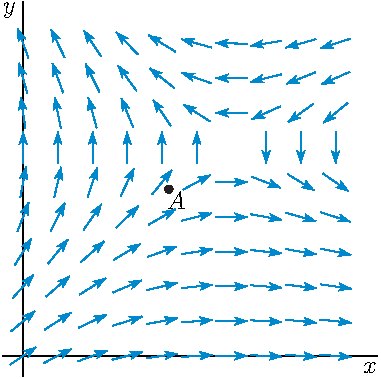
\includegraphics{VFe.pdf}
\end{center}
 Determine the signs of $P$, $Q$, $\pdiff{Q}{x}$
and $\pdiff{Q}{y}$ at the point $A$.
\end{question}

\begin{hint} 
\end{hint}

\begin{answer} 
$P>0$\qquad
$Q>0$\qquad
$\pdiff{Q}{x}<0$\qquad
$\pdiff{Q}{y}>0$
\end{answer}

\begin{solution}
The arrows near the point $A$ are pointing to the
right, indicating that $P>0$, and upward, indicating
that $Q>0$. Moving from left to right near $A$, the
vertical component of the arrows is decreasing, indicating that 
$\pdiff{Q}{x}<0$.  Moving vertically
upwards near $A$, the vertical component of the arrows is 
increasing, indicating that $\pdiff{Q}{y}>0$.

\end{solution}

%%%%%%%%%%%%%%%%%%
\begin{question}
Imagine that the vector field $\vv(x,y) = x\,\hi+y\,\hj$ 
%of part (a) of Q[\ref{prb sketch vf}] 
is the velocity field of a moving fluid.
\begin{enumerate}[(a)]
\item
At time $0$ you drop a twig into the fluid at
the point $(1,1)$. What is the approximate position of the twig
at time $t=0.01$?
\item
At time $0$ you drop a twig into the fluid at
the point $(0,0)$. What is the position of the twig
at time $t=0.01$? 
\item 
At time $0$ you drop a twig into the fluid at
the point $(0,0)$. What is the position of the twig
at time $t=10$?
\end{enumerate}
\end{question}

\begin{hint} 
When the twig is at $(x,y)$ it has velocity $\vv(x,y)$.
\end{hint}

\begin{answer} 
(a) $(1.01\,,\,1.01)$\qquad
(b) $(0\,,\,0)$\qquad
(c) $(0\,,\,0)$
\end{answer}

\begin{solution}
(a) 
At time $0$ the velocity of the twig is
$\vv(1,1) =\hi+\hj$. So at time $t=0.01$, the position of the
twig is approximately
\begin{equation*}
(1,1) + 0.01(1,1) = (1.01\,,\,1.01)
\end{equation*}

(b) 
At time $0$ the velocity of the twig is
$\vv(0,0) =\vZero$. So at time $t=0.01$, the position of the
twig is
\begin{equation*}
(0,0) + 0.01(0,0) = (0\,,\,0)
\end{equation*}

(c) At time $0$ the velocity of the twig is $\vv(0,0) =\vZero$.
So it is stationary and its velocity remains zero for all time.
The position of the twig at time $10$, and in fact at all times,
is $(0\,,\,0)$.

\end{solution}
%%%%%%%%%%%%%%%%%%

%%%%%%%%%%%%%%%%%%
\begin{question}
Imagine that the vector field $\vv(x,y) = 2x\,\hi -\hj$ 
%of part (b) of Q[\ref{prb sketch vf}] 
is the velocity field of a moving fluid.
At time $0$ you drop a twig into the fluid at
the point $(0,0)$. What is the position of the twig
at time $t=10$?
\end{question}

\begin{hint} 
Whenever the twig is on the $y$-axis, its velocity is parallel to the $y$-axis.
So it remains on the $y$-axis for all time.
\end{hint}

\begin{answer} 
$(0\,,\,-10)$
\end{answer}

\begin{solution}
The velocity of the fluid at all points of the $y$-axis
is $-\hj$. So the twig will remain on the $y$-axis and will
consequently have velocity $-\hj$ for all time. The position
of the twig at time $10$ will be
\begin{equation*}
(0,0)+10(0,-1) = (0\,,\,-10)
\end{equation*}
\end{solution}


%%%%%%%%%%%%%%%%%%
\subsection*{\Procedural}
%%%%%%%%%%%%%%%%%%


%%%%%%%%%%%%%%%%%%
\begin{question}
A platform with many small conveyor belts is aligned on a coordinate plane. Every conveyor belt moves an object on top of it in the direction of the origin, and a conveyor belt at position $(x,y)$ causes an object on top of it to move with speed $y$. Assume the objects do not interfere with one another.

 Give a vector-valued formula for the velocity of an object at position $(x,y)$.
 \end{question}

\begin{hint} 
If you know the speed and direction of an object, you can find its velocity.
\end{hint}

\begin{answer} 
$\vv(x,y)=\frac{-y}{\sqrt{x^2+y^2}}(x,y)$
\end{answer}

\begin{solution}

\item  Since all conveyors point towards the origin, the direction of motion of an object at location $(x,y)$ is $\frac{(-x,-y)}{\sqrt{x^2+y^2}}$. Its magnitude is $y$, so $\vv(x,y)=\frac{-y}{\sqrt{x^2+y^2}}(x,y)$.
\end{solution}

\begin{question}
Friendly (?) bees fly towards your face from all directions. The  speed of each bee is inversely proportional to its distance from your face.  Find a vector field for the velocity of the swarm.
\end{question}

\begin{hint} 
Set your face to be at the origin, $(0,0,0)$. 

If $A$ is ``inversely proportional" to $B$, then there exists a constant $\alpha$ such that $AB=\alpha$. That way when $|B|$ goes up, $|A|$ goes down, and vice-versa.
\end{hint}

\begin{answer} 
If your face is at the origin, then $\vv(x,y,z)=-\frac{\alpha}{{x^2+y^2+z^2}}(x,y,z)$ for some positive constant $\alpha$.
\end{answer}

\begin{solution}
Set your face to be at the origin of our coordinate system, $(0,0,0)$. A bee at position $(x,y,z)$ is a distance of $\sqrt{x^2+y^2+z^2}$ from your face, heading in the direction $(-x,-y,-z)$. So, the unit vector indicating the direction of travel of one bee is $\frac{-1}{\sqrt{x^2+y^2+z^2}}(x,y,z)$. Now all we need to find is the length of the velocity vector, i.e. the speed of the bee.

The speed of the friendly bee is inversely proportional to $\sqrt{x^2+y^2+z^2}$, its distance from your face. (Bees that are closer to you are buzzing towards you more excitedly.) So, the speed is given by $\frac{\alpha}{\sqrt{x^2+y^2+z^2}}$ for some constant $\alpha$. 

The bee velocity has the direction of the unit vector $\frac{-1}{\sqrt{x^2+y^2+z^2}}(x,y,z)$ with length  $\frac{\alpha}{\sqrt{x^2+y^2+z^2}}$ for some positive constant $\alpha$. That is,
\[\vv(x,y,z)=-\frac{\alpha}{{x^2+y^2+z^2}}(x,y,z)\]
\end{solution}
%%%%%%%%%%%%%%%%%%

\begin{question}
Sketch the vector field 
$\vv(x,y)=(x^2,y)$.
\end{question}

\begin{hint} 
Start with the regions where $\vv(x,y)\cdot\hi$ and $\vv(x,y)\cdot\hj$ are positive and negative. As you move up/down/left/right, do the vectors get longer or shorter? More horizontal or more vertical?
\end{hint}

\begin{answer} 

\begin{center}
\begin{tikzpicture}
\YEaxis{5}{5}
\foreach \x in {-3,...,3}{\foreach \y in {-4,...,4}{
\POWER{\x}{2}{\xtmp}
\DIVIDE{\xtmp}{10}{\xtmp}%scale 
\ADD{\y}{0}{\ytmp}
\DIVIDE{\ytmp}{10}{\ytmp}%scale
%%we don't want to draw (0,0), so we test x^2+y^2=0. First we find x^2+y^2.
	\POWER{\xtmp}{2}{\xtest}
	\POWER{\ytmp}{2}{\ytest}
	\ADD{\xtest}{\ytest}{\test}
	\ifdim \test pt < 0.01 pt
	\draw[red, thick](\x,\y) --(\x+\xtmp,\y+\ytmp);
	{}
	\else
\draw[->, red, thick] (\x,\y) --(\x+\xtmp,\y+\ytmp);
	\fi
}}
\end{tikzpicture}
\end{center}
\end{answer}

\begin{solution}
Beginning as in the text, we note\\
$\vv(x,y)\cdot\hi=x^2 \begin{cases}
>0 & x \neq 0\\
=0 & x=0
\end{cases}$
\qquad and \qquad
$\vv(x,y)\cdot\hj=y \begin{cases}
>0 & y > 0\\
=0 & y=0\\
<0 & y<0
\end{cases}$ .\\
That leads to the following picture:
\begin{center}
\begin{tikzpicture}
\YEaxis{2.5}{2.5}
\foreach \x in {-1,0,1}{\foreach \y in {-1,0,1}{
\POWER{\x}{2}{\xtmp}
\DIVIDE{\xtmp}{2}{\xtmp} %scale
\ADD{\y}{0}{\ytmp}
\DIVIDE{\ytmp}{2}{\ytmp} %scale
\ifdim\xtmp pt=0pt
\else
\draw[->, blue, thick] (\x,\y) --(\x+\xtmp,\y);
\fi
\ifdim\ytmp pt=0 pt
\else
\draw[->, red, thick] (\x,\y) --(\x,\ytmp+\y);
\fi
}}
\end{tikzpicture}
\end{center}
This gives us a general idea to start with. Refining, we notice that when $x^2>|y|$, then the vector $\vv(x,y)$ will be more horizontal than vertical. As we move away from the $y$-axis in a horizontal line, the difference between $x^2$ and $|y|$ grows, so the vectors get more and more horizontal. However, for a fixed value of $x$, vectors farther from the axis will be more vertical than vectors closer to it.
\begin{center}
\begin{tikzpicture}
\YEaxis{5}{5}
\foreach \x in {-3,...,3}{\foreach \y in {-4,...,4}{
\POWER{\x}{2}{\xtmp}
\DIVIDE{\xtmp}{10}{\xtmp}%scale 
\ADD{\y}{0}{\ytmp}
\DIVIDE{\ytmp}{10}{\ytmp}%scale
%%we don't want to draw (0,0), so we test x^2+y^2=0. First we find x^2+y^2.
	\POWER{\xtmp}{2}{\xtest}
	\POWER{\ytmp}{2}{\ytest}
	\ADD{\xtest}{\ytest}{\test}
	\ifdim \test pt < 0.01 pt
	\draw[red, thick](\x,\y) --(\x+\xtmp,\y+\ytmp);
	{}
	\else
\draw[->, red, thick] (\x,\y) --(\x+\xtmp,\y+\ytmp);
	\fi
}}
\end{tikzpicture}
\end{center}
\end{solution}
%%%%%%%%%%%%%%%%%%%%%%%%%%%%%
\begin{question}
Sketch the \emph{direction} field of
$\vv(x,y) = \left( \sqrt{x^2+y^2}~,~\sqrt{(x-1)^2+(y-1)^2}\right)$.
\end{question}

\begin{hint} 
$\vv(x,y)\cdot \hi$ is the distance from $(x,y)$ to the origin, while $\vv(x,y)\cdot\hj$ is the distance from $(x,y)$ to the point $(1,1)$.
\end{hint}

\begin{answer} 

\begin{tikzpicture}
\YEaaxis{3}{5}{3}{5}
\foreach \x in {-1,-.5,0,.5,1,1.5,2}{\foreach \y in {-1,-.5,0,.5,1,1.5,2}{
\POWER{\x}{2}{\xsquared}
\POWER{\y}{2}{\ysquared}
\ADD{\xsquared}{\ysquared}{\tmp}
\SQUAREROOT{\tmp}{\xtmp}
\DIVIDE{\xtmp}{4}{\xtmp} %scale

%compute vertical
\SUBTRACT{\x}{1}{\xtmpa}
\POWER{\xtmpa}{2}{\xtmpb}
\SUBTRACT{\y}{1}{\ytmpa}
\POWER{\ytmpa}{2}{\ytmpb}
\ADD{\xtmpb}{\ytmpb}{\tmp}
\SQRT{\tmp}{\ytmp}
\DIVIDE{\ytmp}{4}{\ytmp} %scale

%%we don't want to draw (0,0), so we test x^2+y^2=0. First we find x^2+y^2.
	\POWER{\xtmp}{2}{\xtest}
	\POWER{\ytmp}{2}{\ytest}
	\ADD{\xtest}{\ytest}{\test}
	\ifdim \test pt < 0.01 pt
	{} % don't bother with zero vectors
	\else
	\SQUAREROOT{\test}{\L}
	\DIVIDE{\xtmp}{\L}{\xdir}
	\DIVIDE{\ytmp}{\L}{\ydir}
	\DIVIDE{\xdir}{2}{\xdir}%scale
	\DIVIDE{\ydir}{2}{\ydir}%scale
\draw[->, red, thick] (2*\x,2*\y) --(2*\x+\xdir,2*\y+\ydir);
	\fi

}}

\end{tikzpicture}
\end{answer}

\begin{solution}

Although ultimately we'll sketch only unit-length vectors, we can still find the direction of $\vv(x,y)$ by finding its $x$- and $y$ components.

Note $\vv(x,y)\cdot \hi$ is the distance from $(x,y)$ to the origin, while $\vv(x,y)\cdot\hj$ is the distance from $(x,y)$ to the point $(1,1)$. Both these numbers are always nonnegative. This leads to the following sketch:

\begin{center}
\begin{tikzpicture}
\YEaaxis{3}{5}{3}{5}
\foreach \x in {-1,-.5,0,.5,1,1.5,2}{\foreach \y in {-1,-.5,0,.5,1,1.5,2}{
\POWER{\x}{2}{\xsquared}
\POWER{\y}{2}{\ysquared}
\ADD{\xsquared}{\ysquared}{\tmp}
\SQUAREROOT{\tmp}{\xtmp}
\DIVIDE{\xtmp}{4}{\xtmp} %scale
%draw horizontal
\ifdim\xtmp pt=0pt
\else
\draw[->, blue, thick] (2*\x,2*\y) --(2*\x+\xtmp,2*\y);
\fi


%compute vertical
\SUBTRACT{\x}{1}{\xtmpa}
\POWER{\xtmpa}{2}{\xtmpb}
\SUBTRACT{\y}{1}{\ytmpa}
\POWER{\ytmpa}{2}{\ytmpb}
\ADD{\xtmpb}{\ytmpb}{\tmp}
\SQRT{\tmp}{\ytmp}
\DIVIDE{\ytmp}{4}{\ytmp} %scale
%draw vertical
\ifdim\ytmp pt=0 pt
\else
\draw[->, red, thick] (2*\x,2*\y) --(2*\x,\ytmp+2*\y);
\fi
}}
\end{tikzpicture}
\end{center}

When $(x,y)$ is far from the origin, its distance from $(0,0)$ is almost the same as its distance from $(1,0)$. So, we expect $\vv(x,y)$ to be approximately a scalar multiple of $(1,1)$. 

At $(0,0)$, $v(0,0)\cdot \hi=0$, so our vector is horizontal; similarly, $v(1,1)\cdot\hj=0$ so this vector is horizontal. Vectors very near to $(0,0)$ are nearly horizontal, while vectors near to $(1,1)$ are nearly vertical.



\begin{center}
\begin{tikzpicture}
\YEaaxis{3}{5}{3}{5}
\foreach \x in {-1,-.5,0,.5,1,1.5,2}{\foreach \y in {-1,-.5,0,.5,1,1.5,2}{
\POWER{\x}{2}{\xsquared}
\POWER{\y}{2}{\ysquared}
\ADD{\xsquared}{\ysquared}{\tmp}
\SQUAREROOT{\tmp}{\xtmp}
\DIVIDE{\xtmp}{4}{\xtmp} %scale

%compute vertical
\SUBTRACT{\x}{1}{\xtmpa}
\POWER{\xtmpa}{2}{\xtmpb}
\SUBTRACT{\y}{1}{\ytmpa}
\POWER{\ytmpa}{2}{\ytmpb}
\ADD{\xtmpb}{\ytmpb}{\tmp}
\SQRT{\tmp}{\ytmp}
\DIVIDE{\ytmp}{4}{\ytmp} %scale

%%we don't want to draw (0,0), so we test x^2+y^2=0. First we find x^2+y^2.
	\POWER{\xtmp}{2}{\xtest}
	\POWER{\ytmp}{2}{\ytest}
	\ADD{\xtest}{\ytest}{\test}
	\ifdim \test pt < 0.01 pt
	\draw[red, thick](2*\x,2*\y) --(2*\x+\xtmp,2*\y+\ytmp);
	{}
	\else
\draw[->, red, thick] (2*\x,2*\y) --(2*\x+\xtmp,2*\y+\ytmp);
	\fi

}}

\end{tikzpicture}
\end{center}

For the direction field, we normalize our vectors to have unit length.

\begin{center}
\begin{tikzpicture}
\YEaaxis{3}{5}{3}{5}
\foreach \x in {-1,-.5,0,.5,1,1.5,2}{\foreach \y in {-1,-.5,0,.5,1,1.5,2}{
\POWER{\x}{2}{\xsquared}
\POWER{\y}{2}{\ysquared}
\ADD{\xsquared}{\ysquared}{\tmp}
\SQUAREROOT{\tmp}{\xtmp}
\DIVIDE{\xtmp}{4}{\xtmp} %scale

%compute vertical
\SUBTRACT{\x}{1}{\xtmpa}
\POWER{\xtmpa}{2}{\xtmpb}
\SUBTRACT{\y}{1}{\ytmpa}
\POWER{\ytmpa}{2}{\ytmpb}
\ADD{\xtmpb}{\ytmpb}{\tmp}
\SQRT{\tmp}{\ytmp}
\DIVIDE{\ytmp}{4}{\ytmp} %scale

%%we don't want to draw (0,0), so we test x^2+y^2=0. First we find x^2+y^2.
	\POWER{\xtmp}{2}{\xtest}
	\POWER{\ytmp}{2}{\ytest}
	\ADD{\xtest}{\ytest}{\test}
	\ifdim \test pt < 0.01 pt
	{} % don't bother with zero vectors
	\else
	\SQUAREROOT{\test}{\L}
	\DIVIDE{\xtmp}{\L}{\xdir}
	\DIVIDE{\ytmp}{\L}{\ydir}
	\DIVIDE{\xdir}{2}{\xdir}%scale
	\DIVIDE{\ydir}{2}{\ydir}%scale
\draw[->, red, thick] (2*\x,2*\y) --(2*\x+\xdir,2*\y+\ydir);
	\fi

}}

\end{tikzpicture}
\end{center}
\end{solution}

%%%%%%%%%%%%%%%%%%%%%%%%%%%%%%%%%%%%

\begin{question}
Sketch the \emph{direction} field of
$\vv(x,y)=(x^2+xy,y^2-xy)$.
\end{question}

\begin{hint} 
Factor $x^2+xy=x(x+y)$ and $y^2-xy=y(x-y)$.
Chop the plane up into eight regions using the two coordinate axes and the lines $y=x$, $y=-x$.
\end{hint}

\begin{answer} 

\begin{tikzpicture}
\YEaxis{3.5}{3.5}
\foreach \x in {-3,-2.5,...,3.1}{
%compute \vv(x,y)
\POWER{\x}{2}{\xsq}
\foreach \y in {-3,-2.5,...,3.1}{
	\POWER{\y}{2}{\ysq}
	\MULTIPLY{\x}{\y}{\xy}
	\ADD{\xsq}{\xy}{\vx} % vx=x^2+xy
	\SUBTRACT{\ysq}{\xy}{\vy} % vx=y^2-xy
	%compute length
	\POWER{\vx}{2}{\vxsq}
	\POWER{\vy}{2}{\vysq}
	\ADD{\vxsq}{\vysq}{\L}
	\SQUAREROOT{\L}{\l}
	\MULTIPLY{\l}{2}{\l}%scale
	\ifdim \l pt = 0 pt %don't include zero vector at origin
		{}
		\else
		\DIVIDE{\vx}{\l}{\dx}
		\DIVIDE{\vy}{\l}{\dy}
		\draw[thick, red,->] (\x,\y)--(\x+\dx,\y+\dy);
	\fi
}}
\end{tikzpicture}
\end{answer}

\begin{solution}
The sign of $\vv(x,y) \cdot \hi = x(x+y)$ depends on the signs of $x$ and $x+y$. When they have the same signs, $\vv(x,y)\cdot \hi$ is positive, so $\vv(x,y)$ points to the right; when they have different signs, $\vv(x,y)$ points to the left.
\begin{center}
\begin{tikzpicture}
\draw (0,-3)--(0,3) node[above]{$y$};
\draw (-3,3)--(3,-3) node[right]{$y=-x$};
%\fill[pattern color=gray, pattern=north east lines] (-3,3)--(3,-3)|-cycle;
\fill[pattern color=gray, pattern=NE lines, hatch distance=5pt, hatch thickness=0.8pt] (-3,3)--(3,-3)|-cycle;
%\fill[pattern color=gray, pattern=horizontal lines] (0,-3) rectangle (3,3);
\fill[pattern color=gray, pattern=EW lines, hatch distance=5pt, hatch thickness=1.0pt] (0,-3) rectangle (3,3);
\draw[ultra thick, blue,->] (1,0)--(2,0);
\draw[ultra thick, blue,->] (-2,0)--(-1,0);
\draw[very thick, blue,->] (-.5,2)--(-1.5,2);
\draw[very thick, blue,<-] (.5,-2)--(1.5,-2);
\end{tikzpicture}
\end{center}

Similarly, the sign of $\vv(x,y) \cdot \hj = y(y-x)$ depends on the signs of $y$ and $y-x$.
\begin{center}
\begin{tikzpicture}
\draw (-3,0)--(3,0) node[right]{$x$};
\draw (-3,-3)--(3,3) node[right]{$y=x$};
%\fill[pattern color=gray, pattern=north west lines] (-3,-3)--(3,3)-|cycle;
\fill[pattern color=gray, pattern=NW lines, hatch distance=5pt, hatch thickness=1.0pt] (-3,-3)--(3,3)-|cycle;
%\fill[pattern color=gray, pattern=vertical lines] (-3,0) rectangle (3,3);
\fill[pattern color=gray, pattern=NS lines, hatch distance=5pt, hatch thickness=1.0pt] (-3,0) rectangle (3,3);
\draw[ultra thick, red,->] (-1,1)--(-1,2);
\draw[ultra thick, red,->] (1,-2)--(1,-1);
\draw[very thick, red,->] (2,1.5)--(2,.5);
\draw[very thick, red,->] (-2,-.5)--(-2,-1.5);
\end{tikzpicture}
\end{center}

All together:

\begin{center}
\begin{tikzpicture}
\YEaxis{3}{3}
\draw[help lines] (-3,-3)--(3,3) node[right]{$y=x$};
\draw[help lines] (-3,3)--(3,-3) node[right]{$y=-x$};

%equally spaced samples between regions
\foreach \x in {0,...,7}{
	\draw (0,0)+(45*\x+22.5:2.75cm) node[shape=circle,fill, minimum size=1mm, draw, inner sep=0](v\x){};}
\color{blue}%draw x-direction
\foreach \x in {7,0,1,3,4,5} %right arrows
	{\draw(v\x) node[right]{\Large$\rightarrow$};}
\foreach \x in {2,6} %left arrows
	{\draw(v\x) node[left]{\Large$\leftarrow$};}
\color{red}%draw y-direction
\foreach \x in {1,2,3,5,6,7} %up arrows
	{\draw(v\x) node[above]{\Large$\uparrow$};}
\foreach \x in {0,4} %down arrows
	{\draw(v\x) node[below]{\Large$\downarrow$};}
\end{tikzpicture}
\end{center}

Refining, we notice that  as we move straight up or down, $|\vv(x,y)\cdot \hi|$ has its minimum along the lines $y=-x$ and $x=0$. So, the vectors become more strongly vertical as we approach $y=-x$ and $x=0$ from above or below.

Similarly, $|\vv(x,y)\cdot \hj|$ has its minima along the lines $y=x$ and $y=0$, so the vectors become more strongly horizontal as we approach $y=x$ horizontally.

\begin{center}
\begin{tikzpicture}
\YEaxis{3.5}{3.5}
\foreach \x in {-3,-2.5,...,3.1}{
%compute \vv(x,y)
\POWER{\x}{2}{\xsq}
\foreach \y in {-3,-2.5,...,3.1}{
	\POWER{\y}{2}{\ysq}
	\MULTIPLY{\x}{\y}{\xy}
	\ADD{\xsq}{\xy}{\vx} % vx=x^2+xy
	\SUBTRACT{\ysq}{\xy}{\vy} % vx=y^2-xy
	%compute length
	\POWER{\vx}{2}{\vxsq}
	\POWER{\vy}{2}{\vysq}
	\ADD{\vxsq}{\vysq}{\L}
	\SQUAREROOT{\L}{\l}
	\MULTIPLY{\l}{2}{\l}%scale
	\ifdim \l pt = 0 pt %don't include zero vector at origin
		{}
		\else
		\DIVIDE{\vx}{\l}{\dx}
		\DIVIDE{\vy}{\l}{\dy}
		\draw[thick, red,->] (\x,\y)--(\x+\dx,\y+\dy);
	\fi
}}
\end{tikzpicture}
\end{center}
\end{solution}


%%%%%%%%%%%%%%%%%%
%%%%%%%%%%%%%%%%%%


%%%%%%%%%%%%%%%%%%
\begin{question}
Sketch the vector field $\displaystyle \vv(x,y)=\left[\frac{1/3}{\sqrt{x^2+y^2}}(x,y)+\frac{1/3}{\sqrt{(x-1)^2+y^2}}(x-1,y)\right]$.

%Sketch a vector field where there are two very different behaviours whether you are close to the origin or far from it. Something like $x+x^2 $ but more pronounced.

%\[\vv(x,y) = \left( x^2+y^2+\frac{1}{x^2+y^2}~,~\frac{\sqrt{x^2+y^2}}{x^2+y^2+1}\right)\]
%%
\end{question}

\begin{hint} 
What is the geometric interpretation of each summand?
\end{hint}

\begin{answer} 

\begin{tikzpicture}
\YEaxis{5}{5}
\draw (0,0) node[vertex]{};
\draw (1,0) node[vertex]{};

\foreach \x in {-4,-3.5,...,4}{
\foreach \y in {-4,-3.5,...,4}{
	
	\SUBTRACT{\x}{1}{\xless}
	\POWER{\xless}{2}{\xlsq}
	\POWER{\x}{2}{\xsq}
	\POWER{\y}{2}{\ysq}
	\ADD{\xsq}{\ysq}{\xy}
	\ADD{\xlsq}{\ysq}{\xly}
	

		\MULTIPLY{\xy}{\xly}{\testdomain}%%0 if function undefined; otherwise positive
		\SUBTRACT{\x}{.5}{\xtesta}
		\ABSVALUE{\xtesta}{\xtestb}
		\TRUNCATE[0]{\xtestb}{\testzero}%%0 if zero vector; otherwise positive
		\ADD{\testdomain}{\testzero}{\test}%%0 if don't draw; but rounding issues?
		\ifdim \test pt <.1 pt
		{}
		\else %otherwise, finish
		\SQRT{\xy}{\dena}
		\SQRT{\xly}{\denb}
		\DIVIDE{1}{\dena}{\ca}
		\DIVIDE{1}{\denb}{\cb}
		\ADD{\ca}{\cb}{\ymost}
		\MULTIPLY{\ymost}{\y}{\yunscaled}
		\DIVIDE{\yunscaled}{3}{\yy}
		\MULTIPLY{\ca}{\x}{\xa}
		\MULTIPLY{\cb}{\xless}{\xb}
		\ADD{\xa}{\xb}{\xunscaled}
		\DIVIDE{\xunscaled}{3}{\xx}
	
		\draw[red, ->] (\x,\y)--(\x+\xx,\y+\yy);
	\fi
}}
\end{tikzpicture}
\end{answer}

\begin{solution}

The field $\vv(x,y)$ is the sum, scaled by 1/3, of the unit vector pointing away from the origin and the unit vector pointing away from $(1,0)$. This tells us about a few regions:
\begin{itemize}
\item Along the $x$ axis between $(0,0)$ and $(1,0)$, the vectors away from these points are pointing in opposite directions (and have the same length), so they cancel each other out. That is, $v(x,0)=0$ for all $x \in (0,1)$. 
\item $v(0,0)$ and $v(1,0)$ are not defined.
\item Along the $x$-axis outside of $[0,1]$, the vector pointing away from the point $(0,0)$ is the same as the  vector pointing away from the point $(1,0)$. So, $v(x,0)=(-2/3,0)$ for $x<0$ and $v(x,0)=(2/3,0)$ for $x>1$.
\begin{center}
\begin{tikzpicture}
\YEaxis{5}{2}
\draw (0,0) node[vertex]{};
\draw (1,0) node[vertex]{};
\foreach \x in {-4,...,-1}
{\SUBTRACT{\x}{.33}{\xx}
\draw[->, thick, red] (\x,0)--(\xx,0);}
\foreach \x in {2,3,4}
{\ADD{\x}{.33}{\xx}
\draw[->, thick, red] (\x,0)--(\xx,0);}
\end{tikzpicture}
\end{center}
\item As the distance from $(x,y)$ to the origin grows, the vector pointing away from $(0,0)$ looks more and more like the vector pointing away from $(1,0)$. So, our vectors far away from the origin look like vectors of length about 2/3, pointing away from the origin.


\begin{center}
\begin{tikzpicture}
\YEaxis{5}{5}
\draw (0,0) node[vertex]{};
\draw (1,0) node[vertex]{};

\foreach \x in {-4,-3.5,...,4}{
\foreach \y in {-4,-3.5,...,4}{
	
	\SUBTRACT{\x}{1}{\xless}
	\POWER{\xless}{2}{\xlsq}
	\POWER{\x}{2}{\xsq}
	\POWER{\y}{2}{\ysq}
	\ADD{\xsq}{\ysq}{\xy}
	\ADD{\xlsq}{\ysq}{\xly}
	

		\MULTIPLY{\xy}{\xly}{\testdomain}%%0 if function undefined; otherwise positive
		\SUBTRACT{\x}{.5}{\xtesta}
		\ABSVALUE{\xtesta}{\xtestb}
		\TRUNCATE[0]{\xtestb}{\testzero}%%0 if zero vector; otherwise positive
		\ADD{\testdomain}{\testzero}{\test}%%0 if don't draw; but rounding issues?
		\ifdim \test pt <.1 pt
		{}
		\else %otherwise, finish
		\SQRT{\xy}{\dena}
		\SQRT{\xly}{\denb}
		\DIVIDE{1}{\dena}{\ca}
		\DIVIDE{1}{\denb}{\cb}
		\ADD{\ca}{\cb}{\ymost}
		\MULTIPLY{\ymost}{\y}{\yunscaled}
		\DIVIDE{\yunscaled}{3}{\yy}
		\MULTIPLY{\ca}{\x}{\xa}
		\MULTIPLY{\cb}{\xless}{\xb}
		\ADD{\xa}{\xb}{\xunscaled}
		\DIVIDE{\xunscaled}{3}{\xx}
	
		\draw[red, ->] (\x,\y)--(\x+\xx,\y+\yy);
	\fi
}}
\end{tikzpicture}
\end{center}
\end{itemize}
\end{solution}


%%%%%%%%%%%%%%%%%%%%%%%%%%%%%%
\begin{question}\label{prb sketch vf}
Sketch each of the following vector fields, by
drawing a figure like Figure \eref{CLP317}{fig:sourceField} 
in the CLP-4 text.
\begin{enumerate}[(a)]
\item
   $\vv(x,y) = x\,\hi+y\,\hj$.
\item
   $\vv(x,y) = 2x\,\hi -\hj$.
\item
   $\vv(x,y) = \frac{y\,\hi -x\,\hj}{\sqrt{x^2+y^2}}$.
\end{enumerate}
\end{question}

\begin{hint}
(a), (c) Intrepret the vector field geometrically. 
\end{hint}

\begin{answer} 
\begin{center}
      (a) \raisebox{-1.0\height}{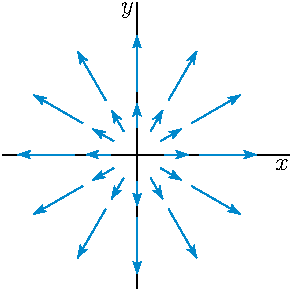
\includegraphics{VFf.pdf}}\qquad
      (b) \raisebox{-1.0\height}{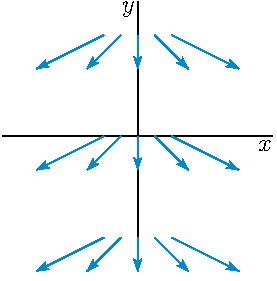
\includegraphics{VFg.pdf}}
\end{center}
\begin{center}
      (c) \raisebox{-1.0\height}{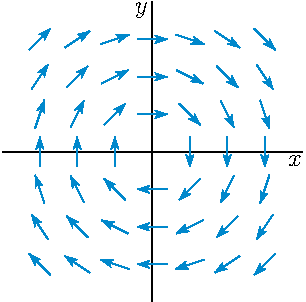
\includegraphics{VFh.pdf}}
\end{center}
\end{answer}

\begin{solution}
(a) 
The vector field $\vv(x,y) = x\,\hi+y\,\hj$ is the same as the radius
vector. It points radially outward and has length growing linearly with
the distance from the origin.
\begin{center}
      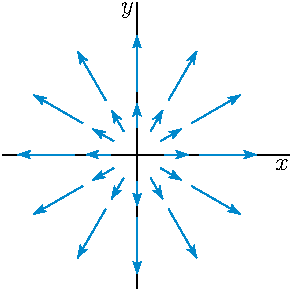
\includegraphics{VFf.pdf}
\end{center}

(b) The vertical component of  $\vv(x,y) = 2x\,\hi -\hj$
is always $-1$. Its horizontal component is $2x$, so that
\begin{itemize}\itemsep1pt \parskip0pt \parsep0pt %\itemindent-15pt
\item
$\vv(x,y)$ is rightward pointing when $x>0$
     and leftward pointing when $x<0$, and
\item
  the magnitude of the horizontal component grows
linearly with the distance from the $y$-axis. 
\end{itemize}
It is sketched in the figure on the left below.
\begin{center}
      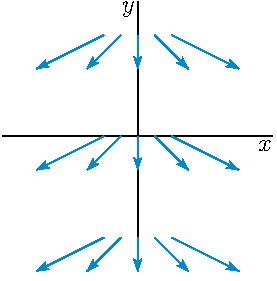
\includegraphics{VFg.pdf}\qquad
      \raisebox{-0.05\height}{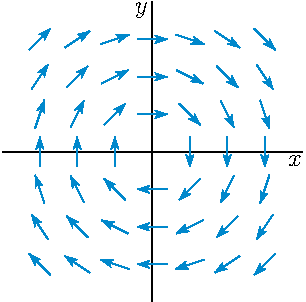
\includegraphics{VFh.pdf}}
\end{center}

(c) For every $(x,y)$ the vector 
               $\vv(x,y) = \frac{y\,\hi -x\,\hj}{\sqrt{x^2+y^2}}$
\begin{itemize}\itemsep1pt \parskip0pt \parsep0pt %\itemindent-15pt
\item
   is of length $1$ and
\item
   is perpendicular to the radius vector $x\,\hi+y\,\hj$.
\item
   $\vv(x,y)$ is rightward pointing when $y>0$
   and leftward pointing when $y<0$, and
\item
   $\vv(x,y)$ is downward pointing when $x>0$
and upward pointing when $x<0$.
\end{itemize}
It is sketched in the figure on the right above.
\end{solution}


%%%%%%%%%%%%%%%%%%
\begin{question}
A body of mass $M$ exerts a force of magnitude $\frac{GM}{D^2}$ on a particle  of unit mass distance $D$ away from itself, where $G$ is a physical constant. The force acts in the direction from the particle to the body.
\begin{center}
\begin{tikzpicture}
\draw (0,0) node[shape=circle, draw]{$M$};
\draw (2,1) node[vertex]{};
\draw[->] (2,1)--(1,.5);
\end{tikzpicture}
\end{center}

Suppose a mass of 5 kg sits at position $(0,0)$, a mass of 3 kg sits at position $(2,3)$, and a mass of 7 kg sits at position $(4,0)$ on a coordinate plane. Give the vector field $\vf(x,y)$ of the net gravitational force exerted on a unit mass at position $(x,y)$. 
\end{question}

\begin{hint} 
The constant $G$ is the same for all masses, but $M$ differs. The net force is the sum of three force vectors.
\end{hint}

\begin{answer} 
$\vf(x,y)=\frac{-5G(x,y)}{(x^2+y^2)^{3/2}}+\frac{3G(2-x,3-y)}{((x-2)^2+(y-3)^2)^{3/2}}+\frac{7G(4-x,-y)}{((x-4)^2+y^2)^{3/2}}
$
\end{answer}

\begin{solution}
A particle of unit mass at position $(x,y)$ has distance $D_1=\sqrt{x^2+y^2}$ from the 5kg mass, so that mass exerts a force of magnitude $\frac{G(5)}{x^2+y^2}$ on the particle. This force has direction $(-x,-y)$. So, the force exerted by the 5kg mass is $\vf_1(x,y)=\frac{-5G}{(x^2+y^2)^{3/2}}(x,y)$.

Similarly, the 3 kg mass at $(2,3)$ exerts a force of $\vf_2(x,y)=\frac{3G}{((x-2)^2+(y-3)^2)^{3/2}}(2-x,3-y)$; and the 7 kg mass at $(4,0)$ exerts a force of $\vf_3(x,y)=\frac{7G}{((x-4)^2+y^2)^{3/2}}(4-x,-y)$.

The net force on a unit mass is therefore
\begin{align*}
\vf(x,y)&=\vf_1(x,y)+\vf_2(x,y)+\vf_3(x,y)\\
&=\frac{-5G(x,y)}{(x^2+y^2)^{3/2}}+\frac{3G(2-x,3-y)}{((x-2)^2+(y-3)^2)^{3/2}}+\frac{7G(4-x,-y)}{((x-4)^2+y^2)^{3/2}}
\end{align*}
\end{solution}
%%%%%%%%%%%%%%%%%%

%%%%%%%%%%%%%%%%%%
\subsection*{\Application}
%%%%%%%%%%%%%%%%%%
%%%%%%%%%%%%%%%%%%
\begin{question}
\begin{enumerate}[a.]
\item 
A pole leans against a vertical wall. The pole has length 2, and it touches the wall at height $H=1$. The pole slides down, still touching the wall, with its height decreasing at a rate of $\diff{H}{t}=0.5$. 


\begin{center}
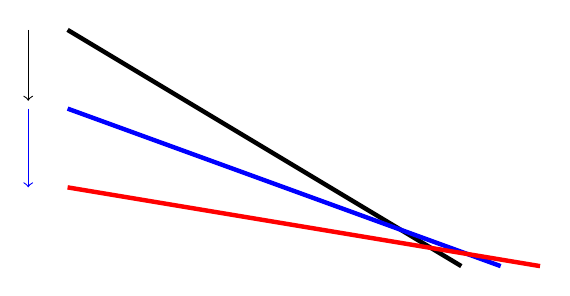
\begin{tikzpicture}
\YEaaxis{.5}{7}{.5}{3.5}
\draw[ultra thick] (5,0)--(0,3);
\draw[->] (-.5,3)--(-.5,2.1);
\color{blue}
\draw[->] (-.5,2)--(-.5,1);
\draw[ultra thick] (5.5,0)--(0,2);
\color{red}
\draw[ultra thick] (6,0)--(0,1);
\end{tikzpicture}
\end{center}
Find a vector function $\vv:\mathbb [0,2] \to \mathbb R^2$ for the velocity, when $H=1$, of a point on the pole that is $p$ units from the lower end, using the coordinate system from the sketch above. 

\item The frame of an umbrella is constructed by attaching straight, rigid poles to a common centre. The poles are all the same length, so they form radii of a circle.

The frame is lifted from the centre of the circle. The edges of the frame drag on the ground, keeping the frame in the shape of a right circular cone that is becoming taller and thinner.

\begin{center}
\begin{tikzpicture}
\draw (0,0) node[vertex]{};
\filldraw[fill opacity=0.2] (0,0)--(-2,-1) arc(180:360:2cm and .75cm)--(0,0);
\draw (0,0)--(-1,-1.65);
\draw (0,0)--(1,-1.65);
\draw[thick,->] (3,-.5)--(4,-.5);
\end{tikzpicture}
\qquad 
\begin{tikzpicture}
\draw (0,0) node[vertex]{};
\filldraw[fill opacity=0.2] (0,0)--(-1,-2) arc(180:360:1cm and .375cm)--(0,0);
\draw (0,0)--(-.5,-2.35);
\draw (0,0)--(.5,-2.35);
\end{tikzpicture}
\end{center}

Suppose the length of each pole is 2 metres, and the centre of the frame is being lifted at a rate of 50 cm/s.  Give a vector field for the velocity $\vV(x,y,z)$ of a point
           $(x,y,z)$ on the frame when its centre is 1 metre above the ground. 

Let the ground have height $z=0$, and let the centre of the frame sit directly above the origin. 
\end{enumerate}
\end{question}

\begin{hint} 
For part a., make a triangle with $P$ as one of its vertices that is similar to the triangle made by the pole, the wall, and the ground. Its hypotenuse has length $p$; let its base be $b$ and its height be $h$. Find a way to translate between $(b,h)$ and $(x,y)$.

For part b., use your answer from part a. Start by describing a point on a pole as its distance from the lower end of the pole, $p$. Then, consider $\diff{z}{t}$ and $\left(\diff{x}{t},\diff{y}{t}\right)$ separately. If you're having a hard time simplifying your answer, note  $\sqrt{x^2+y^2}=\sqrt3(1-z)$ for any point $(x,y,z)$ on a pole when $H=1$.
\end{hint}

\begin{answer} 
a. $\vv(p)=\left( \left(1-\frac{p}{2}\right)\frac{1}{2\sqrt{3}}~,~-\frac{p}{4} \right)$\qquad
b. $\vV(x,y,z)=\left(
-\frac{x}{6}, -\frac{y}{6},\frac{z}{2}\right)$ or equivalent
\end{answer}

\begin{solution}
\begin{enumerate}[a.]
\item Consider a point $P$ on the pole that is a distance $p$ away from the bottom end. Use this point to make a smaller right triangle, as in the picture below.

\begin{center}
\begin{tikzpicture}
\YEaaxis{.5}{5.5}{.5}{3.5}
\draw[thick] (5,0)-|(0,3)--cycle;
\draw (2,2) node[ above]{2};
\draw (-.5,1.5) node{$H$};
\draw (2.5,-1.25) node{$\sqrt{4-H^2}$};
\color{red}
\draw (3,1.2) node[vertex, label=above:{$P$}]{};
\filldraw[fill opacity=0.1](5,0)-|(3,1.2)--cycle;
\draw[|-|] (5.5,.5) --(3.5,1.7) node[midway, above]{$p$};
\draw (4,-.5) node{$b$};
\draw (2.5,.5) node{$h$};
\end{tikzpicture}
\end{center}

Using similar triangles:
\begin{align*}
 h&=\frac{p}{2}H  & b&=\frac{p}{2}\sqrt{4-H^2}
\intertext{If $P$ is at position $(x,y)$, then:}
 y&=h=\frac{p}{2}H & x&=\sqrt{4-H^2}-b=\left(1-\frac{p}{2}\right)\sqrt{4-H^2}\\
\diff{y}{t}&=\frac{p}{2}\diff{H}{t}=-\frac{p}{4}
&\diff{x}{t}&=\left(1-\frac{p}{2}\right)\frac{-H}{\sqrt{4-H^2}}\diff{H}{t}=\left(1-\frac{p}{2}\right)\frac{H}{2\sqrt{4-H^2}}
\intertext{When $H=1$:}
\left.\diff{y}{t}\right|_{H=1}&=-\frac{p}{4}
&\left.\diff{x}{t}\right|_{H=1}&=\left(1-\frac{p}{2}\right)\frac{1}{2\sqrt{3}}
\end{align*}
Therefore,
\[\vv(p)=\left.\left( \diff{x}{t},\diff{y}{t}\right)\right|_{H=1}=\left( \left(1-\frac{p}{2}\right)\frac{1}{2\sqrt{3}}~,~-\frac{p}{4} \right)\]

For our model, we set the domain of this function to be $[0,2]$.


\item 
Let's start by seeing what we can salvage from our work on part a.
As in part a., consider a point $P$ on one of the poles, $p$ metres from the bottom end.
\begin{center}
\begin{tikzpicture}[xscale=1.25]
\draw[thick] (5,0)-|(0,3)--cycle;
\draw (0,3) node[vertex, label=left:{$(0,0,H)$}]{};
\draw[|-|] (6,1)--(1,4) node[midway, above]{2};
\draw[|-|] (0,-.3)--(3,-.3) node[midway, below]{$\sqrt{x^2+y^2}$};
\draw[|-|] (0,-1.25)--(5,-1.25) node[midway, below]{$\sqrt{4-H^2}$};
%\draw (-.5,1.5) node{1};
\color{red}
\draw[thick, red, fill=red, fill opacity=0.1] (5,0)-|(3,1.2)--cycle;
\draw (3,1.2) node[vertex, label=left:{$P=(x,y,z)$}]{};
\draw[|-|] (5.5,.5) --(3.5,1.7) node[midway, above]{$p$};
\end{tikzpicture}
\end{center}

Let $P$ have position $(x,y,z)$. Noting that $\diff{H}{t}$ is now positive, not negative, if we stick to this two-dimensional slice,
\[ \vV(p)=\left( \left(1-\frac{p}{2}\right)\frac{-1}{2\sqrt{3}}~,~\frac{p}{4} \right) \] 
where the second coordinate is $z$ and the first coordinate refers to the (horizontal) line in the direction of the vector $(x,y,0)$.


\begin{center}
\begin{tikzpicture}[scale=2]
\draw[help lines, ->] (0,-1)--(0,1.5) node[above]{$z$};
\draw (0,1) node[vertex, label=above right:{$(0,0,H)$}]{};
\draw (0,1)--(-2,-1) arc(180:360:2cm and .75cm)--(0,1);
\filldraw[fill opacity=0.1] (0,1)--(1,-1.65)--(0,-1)--cycle;
\draw (0,-1) node[vertex, label=left:{$(0,0,0)$}]{};
\draw[->,blue] (0,-1) -- (1.5,-1.98) node[right]{$c\cdot(x,y,0)$};
\color{red}
\fill[opacity=0.2,red] (1,-1.65)--(.66,-.77)--(.66,-1.44)--cycle;
\draw[red, |-|] (.8,-.7)--(1.1,-1.6) node[midway, right]{$p$};
\draw (.66,-.77) node[vertex, label=above right:{$(x,y,z)$}]{};
\draw (.66,-1.44) node[vertex, label= left:{$(x,y,0)$}]{};
\end{tikzpicture}
\end{center}

So, we know $\displaystyle\left.\diff{z}{t}\right|_{H=1}=\frac{p}{4}$, and we know $\displaystyle\left.\left(\diff{x}{t},\diff{y}{t}\right)\right|_{H=1}=(x,y)c$ for some negative constant $c$ with $|(x,y)c|=\left(1-\frac{p}{2}\right)\frac{1}{2\sqrt{3}}$. Since we have the direction and the magnitude of the vector, we can find the vector:
\[\left.\left( \diff{x}{t},\diff{y}{t}\right)\right|_{H=1}=(x,y)c=-\frac{\left(1-\frac{p}{2}\right)}{2\sqrt 3\sqrt{x^2+y^2}}(x,y)
\]

We want our equation to be in terms of $x$, $y$, and $z$, so we need to get rid of $p$.
Using similar triangles, $\frac{p}{2}=\frac{\sqrt{4-H^2}-\sqrt{x^2+y^2}}{\sqrt{4-H^2}}$. When $H=1$, then $1-\frac{p}{2}=\frac{\sqrt{x^2+y^2}}{\sqrt3}$. So:

\[\left.\left( \diff{x}{t},\diff{y}{t}\right)\right|_{H=1}
=-\frac{1}{6}(x,y)\]

Finally:
\[\vV(x,y,z)=\left.\left( \diff{x}{t},\diff{y}{t},\diff{z}{t}\right)\right|_{H=1}=\left(
-\frac{1}{6}x~,~
-\frac{1}{6}y~,~
\frac{1}{2}z\right)\]

Not all values of $(x,y,z)$ are on the frame. But, for those values of $(x,y,z)$ that \emph{are} on the frame, this equation holds.

\end{enumerate}
\end{solution}
%%%%%%%%%%%%%%%%%%
%%%%%%%%%%%%%%%%%%

\section{Field Lines}
%\documentclass[12pt]{article}

\questionheader{ex:s2.2}

%%%%%%%%%%%%%%%%%%
%\subsection*{\Conceptual}
%%%%%%%%%%%%%%%%%%


\begin{question}
Suppose that the vector field $\vv(x,y)$ sketched below represents the velocity of 
moving water at the point $(x,y)$ in the first quadrant of the $xy$-plane.
  \begin{center}
       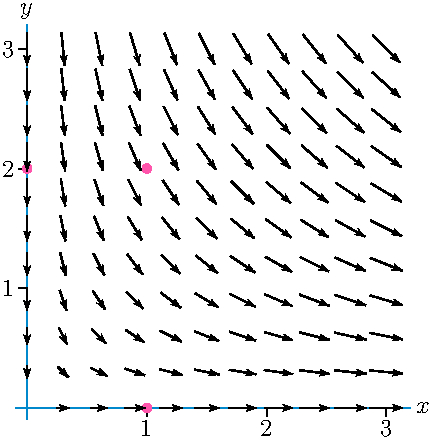
\includegraphics{duckyField.pdf}
  \end{center}
Sketch the path followed by a rubber ducky dropped in at the point
\begin{enumerate}[(a)]
\item $(0,2)$
\item $(1,0)$
\item $(1,2)$
\end{enumerate}
%Describe its velocity as it changes position.
\end{question}

%\begin{hint} 
%\end{hint}

\begin{answer} 
\begin{center}
       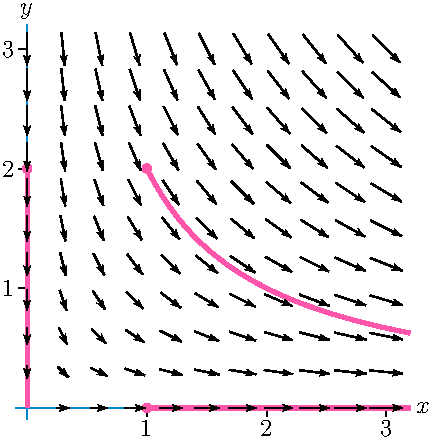
\includegraphics{duckyField2.pdf}
  \end{center}
\end{answer}

\begin{solution}
(a) At every point of the positive $y$-axis, the velocity vector $\vv(0,y)$
points straight down. So a rubber ducky placed in the water at $(0,2)$
just floats straight down the positive $y$-axis towards the origin.

\begin{center}
       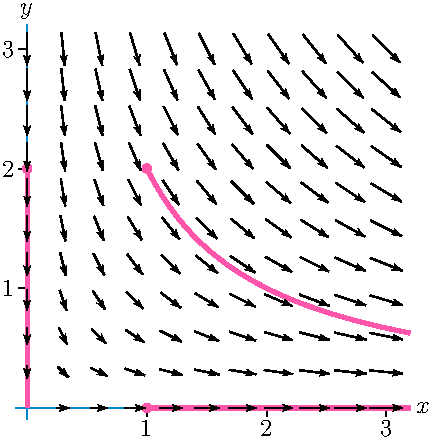
\includegraphics{duckyField2.pdf}
  \end{center}

\noindent
(b) At every point of the positive $x$-axis, the velocity vector $\vv(x,0)$
points straight to the right. So a rubber ducky placed in the water at $(1,0)$
just floats rightward along the positive $x$-axis.

\noindent
(c) At every point of the first quadrant away from the axes, the 
velocity vector $\vv(x,y)$ points downwards and towards the right. So a 
rubber ducky placed in the water at $(1,2)$ always floats down and to 
the right. The closer the ducky gets to the $x$--axis the more rightward 
its motion becomes. 

\end{solution}


\begin{question}
Find a vector field $\vv(x,y)$ for which
\begin{align*}
x(t) &= e^{-t}\cos t \\
y(t) &= e^{-t}\sin t \\
\end{align*}
is a field line.
\end{question}

\begin{hint} 
Express $x'(t)$ and $y'(t)$ purely in terms of $x(t)$ and $y(t)$.
\end{hint}

\begin{answer} 
$\vv(x,y) = (-x-y\,,\,x-y)$
\end{answer}

\begin{solution}
The derivatives
\begin{alignat*}{3}
x'(t) &= -e^{-t}\cos t - e^{-t}\sin t &&= -x(t)-y(t) \\
y'(t) &= -e^{-t}\sin t + e^{-t}\cos t &&= -y(t)+x(t) 
\end{alignat*}
So $\big(x(t),y(t)\big)$ is a solution of the system of differential equations
\begin{align*}
\diff{x}{t} &= v_1(x,y) = -x-y \\
\diff{y}{t} &= v_2(x,y) = \phantom{-}x-y
\end{align*}
So the vector field is $\vv(x,y) = \big(v_1(x,y)\,,\,v_2(x,y)\big) 
                                 = (-x-y\,,\,x-y)$.
\end{solution}




%\begin{question}
%The direction field shown below represents the differential equation blah. If the initial condition is $y=blah$, what is $\lim\limits_{t \to \infty} y$?
%\end{question}
%
%\begin{hint} 
%\end{hint}
%
%\begin{answer} 
%\end{answer}
%
%\begin{solution}
%\end{solution}



%%%%%%%%%%%%%%%%%%
\subsection*{\Procedural}
%%%%%%%%%%%%%%%%%%

\begin{question}[M317 2010A] %1
Consider the function $f(x,y) = xy$.
\begin{enumerate}[(a)]
\item
Explicitly determine the field lines (flow lines) of 
$\vF(x,y) = \vnabla f$.
\item
Sketch the field lines of $\vF$ and the level curves of $f$ in the same diagram.
\end{enumerate}
\end{question}

\begin{hint} 
Review \S\eref{CLP317}{sec:fieldLines} in the CLP-4 text.
\end{hint}

\begin{answer} 
(a) $\frac{x^2}{2} =\frac{y^2}{2} +C$

(b) 
  \begin{center}
       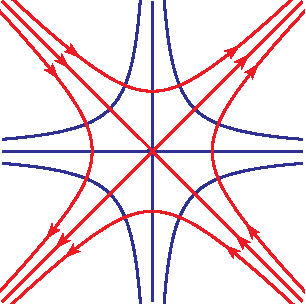
\includegraphics{OE10A_1.pdf}
  \end{center}

\end{answer}

\begin{solution} (a) The field lines of $\vF(x,y) = \vnabla f
=y\,\hi + x\,\hj$ obey
\begin{align*}
\frac{\dee{x}}{y} = \frac{\dee{y}}{x}
\iff x\,\dee{x} = y\,\dee{y}
\iff \frac{x^2}{2} =\frac{y^2}{2} +C
\end{align*}
for any constant $C$.

\noindent (b)
The sign data
\begin{align*}
\hi\cdot\vF(x,y) = y
    \left.\begin{cases}
             >0 &\text{if $y>0$} \\
             =0 &\text{if $y=0$} \\
             <0 &\text{if $y<0$} 
       \end{cases}\right\}\qquad
\hj\cdot\vF(x,y) = x
    \left.\begin{cases}
             >0 &\text{if $x>0$} \\
             =0 &\text{if $x=0$} \\
             <0 &\text{if $x<0$} 
       \end{cases}\right\}\qquad
\end{align*}
is visually displayed in the figure on the left below. The arrows in the
figure on the left gives us the direction of motion along 
the field lines $\frac{x^2}{2} =\frac{y^2}{2} +C$ (in red) in the 
figure on the right below. Some equipotential curves $xy=C$ are 
also sketched (in blue) in the figure on the right below.

  \begin{center}
       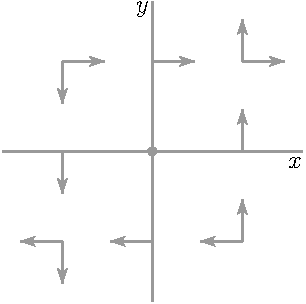
\includegraphics{OE10A_1Sign.pdf}\qquad\qquad
       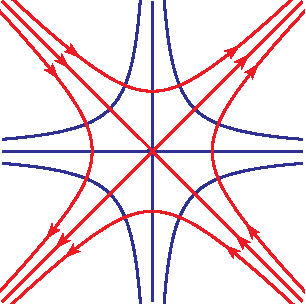
\includegraphics{OE10A_1.pdf}
  \end{center}


\end{solution}

%%%%%%%%%%%%%%%%%%%%%%%%%%%
\begin{question}[M317 2003A] %1
Find the field line of the vector field
$\vF= 2y\,\hi+ \frac{x}{y^2}\,\hj+e^y\hk$ that passes through
$(1,1,e)$.
\end{question}

%\begin{hint} 
%\end{hint}

\begin{answer} 
$x=y^2$, $z=e^y$
\end{answer}

\begin{solution} 
The field lines obey
\begin{equation*}
\frac{\dee{x}}{2y}=\frac{\dee{y}}{x/y^2}=\frac{\dee{z}}{e^y}
\qquad\text{ if $x,y\ne 0$}
\end{equation*}
In particular
\begin{align*}
\frac{\dee{x}}{2y}=\frac{y^2\,\dee{y}}{x}
\implies
x\,\dee{x}=2y^3\,\dee{y}
\implies
\frac{1}{2}x^2=\frac{1}{2}y^4+C
\end{align*}
Since $y=1$ when $x=1$, $C=0$. So $x=y^2$ and
\begin{equation*}
\frac{\dee{y}}{x/y^2}=\frac{\dee{z}}{e^y}
\implies
e^ydy=dz
\implies
z=e^y+D
\end{equation*}
Since $z=e$ when $y=1$, $D=0$. So the field line is
\begin{equation*}
x=y^2 \qquad z=e^y
\end{equation*}
\end{solution}

%%%%%%%%%%%%%%%%%%%%%%%%%%%
\begin{question}[M317 2001A] %1
 Find and sketch the field lines of the vector field
$\vF= x\,\hi+ 3y\,\hj$.
\end{question}

%\begin{hint} 
%\end{hint}

\begin{answer}
The field lines are $y=C'x^3$ with $C'$ a nonzero constant,
as well as $x=0$ and $y=0$.

\begin{center}
   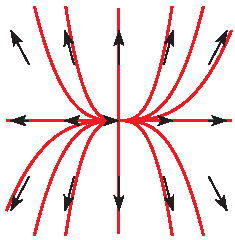
\includegraphics{fline.pdf}
\end{center}

\end{answer}

\begin{solution} 
 The field lines obey
\begin{align*}
&\frac{\dee{x}}{x}=\frac{\dee{y}}{3y}\qquad\text{ if $x,y\ne 0$}\\
&\implies 3\ln |x|=\ln |y|+C\\
&\implies |x|^3=e^C|y| \\
&\implies y=\pm e^{-C}x^3 \\
&\implies y=C'x^3
\end{align*}
with $C'$ a nonzero constant.
$x=0$ and $y=0$ are also field lines,
since on the $y$-axis $\vF\parallel\hj$ and
on the $x$-axis $\vF\parallel\hi$.

\begin{center}
   \includegraphics{fline.pdf}
\end{center}
\end{solution}




%%%%%%%%%%%%%%%%%%
%\subsection*{\Application}
%%%%%%%%%%%%%%%%%%


\section{Conservative Vector Fields}
%\documentclass[12pt]{article}

\questionheader{ex:s2.3}

%%%%%%%%%%%%%%%%%%
\subsection*{\Conceptual}
%%%%%%%%%%%%%%%%%%

%%%%%%%%%%%%%%%%%%
\begin{question}
We've seen two calculations of the energy $E$ of a system. Equation~\eref{CLP317}{eqn:consEnergy} told us
$E=\frac{1}{2}m|\vv|^2+mgy$, while Example~\eref{CLP317}{eg:potentialEnergy} says $\frac{1}{2} m |\vv(t)|^2 -\varphi\big(x(t),y(t),z(t)\big)=E$.

Consider a force given by $\vF = \vnabla \varphi$ for some differentiable function $\varphi:\mathbb R^3 \to \mathbb R$. A particle of mass $m$ is being acted on by $\vF$ and no other forces, and its position at time $t$ is given by $(x(t),y(t),0)$.

True or false: $mgy(t)=-\varphi(x(t),y(t),0)$.
\end{question}
\begin{hint}
Carefully consider the context that lead to each of these equations.
\end{hint}
\begin{answer}
In general, false.
\end{answer}
\begin{solution}
False, in general.

In the context of Equation~\eref{CLP317}{eqn:consEnergy}, the only forces acting on the particle are gravity, $-mg\hj$, and the normal force, $W\hN$.

We make no such constraints on the force in Example~\eref{CLP317}{eg:potentialEnergy}. Certainly $\vF$ \emph{could} arise from gravity and the normal force of a track, but there's nothing saying it has to. For example, suppose $\varphi$ is an equation that does not depend on $m$ and/or $g$. Alternately, suppose the $y$-coordinate of our three-dimensional system is not ``up."
\end{solution}

%%%%%%%%%%%%%%%%%%%

\begin{question}
For each of the following fields, decide which of the following holds:
\begin{enumerate}[A.]
\item The screening test for conservative vector fields tells us $\vF$ is conservative.
\item The screening test for conservative vector fields tells us $\vF$ is \textbf{not} conservative.
\item The screening test for conservative vector fields does not tell us whether $\vF$ is conservative or not.
\end{enumerate}
(The screening test is Theorem~\eref{CLP317}{thm:screen} in the text.)

\begin{enumerate}[a.]
\item $\vF=x\hi + z\hj + y\hk$
\item $\vF=y^2z\hi + x^2z\hj + x^2y\hk$
\item $\vF=(ye^{xy}+1)\hi + (xe^{xy}+z)\hj + \left( \frac1z+y\right)\hk$
\item $\vF=y\cos(xy)\hi + x\sin(xy)\hj $
\end{enumerate}
\end{question}
\begin{hint}
One of the three options will NEVER be true, for any $\vF$.
\end{hint}
\begin{answer}
a. C \qquad
b. B \qquad
c. C \qquad
d. B 
\end{answer}
\begin{solution}
Remember that the screening test can only rule out conservativity --- it can never, by itself, guarantee conservativity. So, A is \emph{never} the case.
\begin{enumerate}[a.]
\item \begin{align*}\vF&=x\hi + z\hj + y\hk\\
\vnabla \times \vF&=\Big(\pdiff{F_3}{y} -\pdiff{F_2}{z} \Big)\hi
+\Big(\pdiff{F_1}{z} -\pdiff{F_3}{x} \Big)\hj
+\Big(\pdiff{F_2}{x} -\pdiff{F_1}{y} \Big)\hk\\
&=(1-1)\hi+(0-0)\hj+(0-0)\hk = \mathbf0
\end{align*}
This field passes the screening test. That means the screening test doesn't rule out the possibility of $\vF$ being conservative. So, we have option C.

\item  \begin{align*}\vF&=y^2z\hi + x^2z\hj + x^2y\hk\\
\vnabla \times \vF&=\Big(\pdiff{F_3}{y} -\pdiff{F_2}{z} \Big)\hi
+\Big(\pdiff{F_1}{z} -\pdiff{F_3}{x} \Big)\hj
+\Big(\pdiff{F_2}{x} -\pdiff{F_1}{y} \Big)\hk\\
&=(x^2-x^2)\hi+(y^2-2xy)\hj+(2xz-2yz)\hk \neq \mathbf0
\end{align*}
So, $\vF$ fails the screening test --- it's not conservative. That's option B.

\item 
 \begin{align*}\vF&=(ye^{xy}+1)\hi + (xe^{xy}+z)\hj + \left( \frac1z+y\right)\hk\\
\vnabla \times \vF&=\Big(\pdiff{F_3}{y} -\pdiff{F_2}{z} \Big)\hi
+\Big(\pdiff{F_1}{z} -\pdiff{F_3}{x} \Big)\hj
+\Big(\pdiff{F_2}{x} -\pdiff{F_1}{y} \Big)\hk\\
&=(1-1)\hi+(0-0)\hj+(e^{xy}(xy+1)-e^{xy}(xy+1))\hk = \mathbf0
\end{align*}
$\vF$ passes the screening test, so it may or may not be conservative. That is Option C.

\item
 \begin{align*}\vF&=y\cos(xy)\hi + x\sin(xy)\hj \\
\pdiff{F_2}{x}&=xy\cos(xy)+\sin(xy)\\
\pdiff{F_1}{y}&=-xy\sin(xy)+\cos(xy)\\
\pdiff{F_2}{x}&\neq \pdiff{F_1}{y}
\end{align*}
$\vF$ fails the screening test, so it is not conservative.
That is Option B.

\end{enumerate}
\end{solution}

%%%%%%%%%%%%%%%%%%%
\begin{question}
Suppose $\vF$ is conservative and let $a$, $b$, and $c$ be constants. Find a potential for $\vF+(a,b,c)$, OR give a conservative field $\vF$ and constants  $a$, $b$, and $c$ for which $\vF+(a,b,c)$ is not conservative.

\end{question}
\begin{hint}
Modify $\varphi$, the potential for $\vF$.
\end{hint}
\begin{answer}
Let $\varphi$ be a potential for $\vF$. Define $\phi=\varphi+ax+by+cz$. Then $\vnabla \phi = \vnabla\varphi+(a,b,c)=\vF+(a,b,c)$.
\end{answer}
\begin{solution}
Let $\varphi$ be a potential for $\vF$. Define $\phi=\varphi+ax+by+cz$. Then $\vnabla \phi = \vnabla\varphi+(a,b,c)=\vF+(a,b,c)$. So, $\vF+(a,b,c)$ is also conservative.
\end{solution}

%%%%%%%%%%%%%%%%%%%
\begin{question}
Prove, or find a counterexample to, each of the following statements.
\begin{enumerate}[a.]
\item
If $\vF$ is a conservative field and $\vG$ is  a non-conservative field, then $\vF+\vG$ is non-conservative.
\item
If $\vF$ and $\vG$ are both non-conservative fields, then $\vF+\vG$ is non-conservative.
\item If $\vF$ and $\vG$ are both conservative fields, then $\vF+\vG$ is conservative.

\end{enumerate}
\end{question}
\begin{hint}
a. If $\vF+\vG$ is conservative, what has to be true?\\
b. What if $\vF$ and $\vG$ are quite similar?\\
c. Find a potential for $\vF+\vG$.
\end{hint}
\begin{answer}
\begin{enumerate}[a.]
\item If $\vF+\vG$ is \emph{conservative} for any particular $\vF$ and $\vG$, then by definition, there exists a potential $\varphi$ with $\vF+\vG = \vnabla \varphi$. 

Since $\vF$ is conservative, there also exists a potential $\psi$ with $\vF = \vnabla \psi$.

But now $\vG = (\vF+\vG)-\vF=\vnabla \varphi - \vnabla \psi = \vnabla(\varphi-\psi)$. That means the function $(\varphi-\psi)$ is a potential for $G$. However, this is impossible: since $\vG$ is non-conservative, no function with this property exists.

So it is not possible that $\vF+\vG$ is conservative. It must be non-conservative.
\item Counterexample: if $\vF = -\vG$, then $\vF+\vG = \mathbf 0 = \vnabla c$ for any constant $c$.
\item Since both fields are conservative, they both have potentials, say $\vF=\vnabla \varphi$ and $\vG = \vnabla \psi$. Then $\vF+\vG = \vnabla\varphi+\vnabla\psi=\vnabla(\varphi+\psi)$. That is, $(\varphi+\psi)$ is a potential for $\vF+\vG$, so $\vF+\vG$ is conservative.

\end{enumerate}
\end{answer}
\begin{solution}
\begin{enumerate}[a.]
\item If $\vF+\vG$ is \emph{conservative} for any particular $\vF$ and $\vG$, then by definition, there exists a potential $\varphi$ with $\vF+\vG = \vnabla \varphi$. 

Since $\vF$ is conservative, there also exists a potential $\psi$ with $\vF = \vnabla \psi$.

But now $\vG = (\vF+\vG)-\vF=\vnabla \varphi - \vnabla \psi = \vnabla(\varphi-\psi)$. That means the function $(\varphi-\psi)$ is a potential for $G$. However, this is impossible: since $\vG$ is non-conservative, no function with this property exists.

So it is not possible that $\vF+\vG$ is conservative. It must be non-conservative.
\item Counterexample: if $\vF = -\vG$, then $\vF+\vG = \mathbf 0 = \vnabla c$ for any constant $c$.
\item Since both fields are conservative, they both have potentials, say $\vF=\vnabla \varphi$ and $\vG = \vnabla \psi$. Then $\vF+\vG = \vnabla\varphi+\vnabla\psi=\vnabla(\varphi+\psi)$. That is, $(\varphi+\psi)$ is a potential for $\vF+\vG$, so $\vF+\vG$ is conservative.

\end{enumerate}
\end{solution}
%%%%%%%%%%%%%%%%%%%%%%%%%%%%%%%%%%%%%%
%%%%%%%%%%%%%%%%%%%%%%%%%%%%%%%%%%%%%%%%%%%%%%%%%%%%%%%%%
%%%%%%%%%%%%%%%%%%%
%%%%%%%%%%%%%%%%%%%

%%%%%%%%%%%%%%%%%%
\subsection*{\Procedural}
%%%%%%%%%%%%%%%%%%


%%%%%%%%%%%%%%%%%%%%%%%%%%%
\begin{question}[M317 2006A] %3
Let $D$ be the domain consisting of all $(x,y)$ such that $x>1$,
and let $\vF$ be the vector field
\begin{align*}
\vF =  -\frac{y}{x^2+y^2}\,\hi + \frac{x}{x^2+y^2}\,\hj
\end{align*}
Is $\vF$ conservative on $D$? Give reasons for your answer.

\end{question}

\begin{hint} 
Note that the domain is $D=\Set{(x,y)}{x>1}$. Compare to Example~\eref{CLP317}{eg:screeningCounterexample} in the text.
\end{hint}

\begin{answer} 
Yes, $\vF$ is conservative on $D$. A potential is 
$\varphi(x,y) = \arctan\frac{y}{x}$.
\end{answer}

\begin{solution}
Set $\varphi(x,y)= \arctan\frac{y}{x}$ (using the standard $\arctan$
that takes values between $-\frac{\pi}{2}$ and $\frac{\pi}{2}$). 
Note that $\varphi(x,y)$ is well-defined, with all partial derivatives 
continuous, on $D$ since $x>1$ there. Then
\begin{alignat*}{3}
\pdiff{\varphi}{x}(x,y) 
&= \frac{-\frac{y}{x^2}}{1+\big(\frac{y}{x}\big)^2}
&&= -\frac{y}{x^2+y^2} \\
\pdiff{\varphi}{y}(x,y)  
&= \frac{\frac{1}{x}}{1+\big(\frac{y}{x}\big)^2}
&&= \phantom{-} \frac{x}{x^2+y^2}
\end{alignat*}
so that $\vF=\vnabla\varphi$.
\end{solution}


%%%%%%%%%%%%%%%%%%%%%%%%%%%

%%%%%%%%%%%%%%%%%%%
\begin{question}
Find a potential $\varphi$ for $\vF(x,y)=(x+y)\hi+(x-y)\hj$, or prove none exists.
\end{question}
\begin{hint}
A potential does exist.
\end{hint}
\begin{answer}
$\varphi=\frac{1}{2}x^2+xy-\frac{1}{2}y^2$
\end{answer}
\begin{solution}
If $\varphi$ is a potential for $\vF$, then:
\begin{itemize}
\item $\pdiff{\varphi}{x}=x+y$, so $\varphi = \frac{1}{2}x^2+xy+\psi_1(y)$
\item $\pdiff{\varphi}{y}=x-y$, so $\varphi = xy-\frac{1}{2}y^2+\psi_2(x)$
\end{itemize}
So, for instance, $\varphi = \frac{1}{2}x^2+xy-\frac{1}{2}y^2$ is a potential for $\vF$.
\end{solution}


%%%%%%%%%%%%%%%%%%%
\begin{question}
Find a potential $\varphi$ for $\vF(x,y)=\left( \frac{1}{x}-\frac{1}{y}\right)\hi+\left(\frac{x}{y^2}\right)\hj$, or prove none exists.
\end{question}
\begin{hint}
Recall $\diff{}{x} \ln |x| = \frac1x$.
\end{hint}
\begin{answer}
$\varphi=\ln |x| - \frac{x}{y}$
\end{answer}
\begin{solution}
If $\varphi$ is a potential for $\vF$, then:
\begin{itemize}
\item $\pdiff{\varphi}{x}=\frac1x-\frac1y$, so $\varphi = \ln|x|-\frac{x}{y}+\psi_1(y)$
\item $\pdiff{\varphi}{y}=\frac{x}{y^2}$, so $\varphi = -\frac{x}{y}+\psi_2(x)$
\end{itemize}
So, for instance, $\varphi=\ln |x| - \frac{x}{y}$ is a potential for $\vF$.

\end{solution}


%%%%%%%%%%%%%%%%%%%
\begin{question}
Find a potential $\varphi$ for $\vF(x,y,z)=\left(x^2yz+xz\right)\hi+\left( \frac13x^3z+y \right)\hj+\left(\frac13x^3y+\frac12x^2+y\right)\hk$, or prove none exists. %fails test
\end{question}
\begin{hint}
Try the screening test, Theorem~\eref{CLP317}{thm:screen}.
\end{hint}
\begin{answer}
None exists: $\pdiff{F_2}{z}=\frac13x^3$, while $\pdiff{F_3}{y}=\frac{1}{3}x^3+1$, so $\vF$ fails the screening test, Theorem~\eref{CLP317}{thm:screen}.
\end{answer}
\begin{solution}
None exists: $\pdiff{F_2}{z}=\frac13x^3$, while $\pdiff{F_3}{y}=\frac{1}{3}x^3+1$, so $\vF$ fails the screening test, Theorem~\eref{CLP317}{thm:screen}.
\end{solution}

%%%%%%%%%%%%%%%%%%%
\begin{question}
Find a potential $\varphi(x,y,z)$ for \[\vF(x,y,z)=\left( \frac{x}{x^2+y^2+z^2}\right)\hi+\left( \frac{y}{x^2+y^2+z^2}\right)\hj+\left( \frac{z}{x^2+y^2+z^2}\right)\hk,\] or prove none exists. 
\end{question}
\begin{hint}
$\displaystyle\int\frac{x}{x^2+y^2+z^2}\,\dee{x}$ can be evaluated by inspection, or with the substitution \\$u=x^2+y^2+z^2$.
\end{hint}
\begin{answer}
$\varphi(x,y,z) = \frac12\ln(x^2+y^2+z^2)$
\end{answer}
\begin{solution}
If $\varphi(x,y,z)$ is a potential for $\vF(x,y,z)$, then:
\begin{itemize}
\item $\pdiff{\varphi}{x}(x,y,z)=\frac{x}{x^2+y^2+z^2}$, so $\varphi(x,y,z) = \frac12\ln(x^2+y^2+z^2)+\psi_1(y,z)$
\item $\pdiff{\varphi}{y}(x,y,z)=\frac{y}{x^2+y^2+z^2}$, so $\varphi(x,y,z) = \frac12\ln(x^2+y^2+z^2)+\psi_2(x,z)$
\item $\pdiff{\varphi}{z}(x,y,z)=\frac{z}{x^2+y^2+z^2}$, so $\varphi(x,y,z) = \frac12\ln(x^2+y^2+z^2)+\psi_2(x,y)$
\end{itemize}
So, for instance, $\varphi(x,y,z)= \frac{1}{2}\ln(x^2+y^2+z^2)$ is a potential for $\vF(x,y,z)$.

\end{solution}

%%%%%%%%%%%%%%%%%%%
\begin{question}
Determine whether or not each of the following vector
fields are conservative. Find the potential if it is.
\begin{enumerate}[(a)]
\item
   $\vF(x,y,z)=x\hi-2y\hj+3z\hk$
\item
   $\vF(x,y)=\frac{x\hi-y\hj}{x^2+y^2}$
\end{enumerate}
\end{question}

%\begin{hint}
%\end{hint}

\begin{answer}
(a) $\vF$ is conservative with potential 
   $\phi(x,y,z)=\half x^2-y^2+\frac{3}{2}z^2+C$ for any constant $C$.

(b) $\vF$ is not conservative.
\end{answer}
\begin{solution}
(a) We shall show that $\vF(x,y,z)$ is conservative
by finding a potential for it. $\varphi(x,y,z)$ is a potential for this $\vF$ 
if and only if
\begin{align*}
\pdiff{\varphi}{x}(x,y,z) &= x \\
\pdiff{\varphi}{y}(x,y,z) &= -2y \\
\pdiff{\varphi}{z}(x,y,z) &= 3z
\end{align*}
Integrating the first of these equations gives
\begin{equation*}
\varphi(x,y,z) = \frac{x^2}{2} + f(y,z)
\end{equation*}
Substituting this into the second equation gives 
\begin{equation*}
\pdiff{f}{y}(y,z) 
   = -2y 
\end{equation*}
which integrates to
\begin{equation*}
f(y,z) = -y^2+ g(z)
\end{equation*}
Finally, substituting $\varphi(x,y,z) = \frac{x^2}{2} -y^2 + g(z)$
into the last equation gives
\begin{equation*}
 g'(z) = 3z
\end{equation*}
which integrates to
\begin{equation*}
g(z) = \frac{3}{2} z^2 +C
\end{equation*}
with $C$ being an arbitrary constant.
So, $\vF(x,y,z)$ is conservative and
$\varphi(x,y,z)=\half x^2-y^2+\frac{3}{2}z^2$ is one allowed potential.

(b) 
The field $\vF= F_1\,\hi + F_2\,\hj$ can be conservative 
only if it passes the screening test
\begin{equation*}
\pdiff{F_1}{y}=\pdiff{F_2}{x}
\end{equation*}
In this case
\begin{equation*}
\pdiff{F_1}{y}
=\frac{\partial\hfill}{\partial y}\Big(\frac{x}{x^2+y^2}\Big)
=-\frac{2xy}{{(x^2+y^2)}^2}
\end{equation*}
is different from 
\begin{equation*}
\pdiff{F_2}{x}
=\frac{\partial\hfill}{\partial x}\Big(\frac{-y}{x^2+y^2}\Big)
=\frac{2xy}{{(x^2+y^2)}^2}
\end{equation*}
for all $(x,y)$ with $x$ and $y$ both nonzero.
So $\vF$ is not conservative.
\end{solution}



%%%%%%%%%%%%%%%%%%%
\begin{question}
Let 
$\vF= e^{(z^2)}\,\hi+2Byz^3\,\hj
          +\big(Axze^{(z^2)}+3By^2z^2\big)\,\hk$.
\begin{enumerate}[(a)]
\item
For what values of the constants $A$ and $B$ is the
vector field $\vF$ conservative on $\bbbr^3$?
\item
If $A$ and $B$ have values found in (a),
    find a potential function for $\vF$.
\end{enumerate}
\end{question}

\begin{hint}
For what values of the constants $A$ and $B$ does the
vector field $\vF$ pass the screening test
$\vnabla\times\vF=\vZero$?
\end{hint}

\begin{answer}
(a)
$A=2$, $B$ is arbitrary.

(b)
$\varphi(x,y,z)=xe^{(z^2)}+By^2 z^3+C$
for any constant $C$.
\end{answer}

\begin{solution}
By Theorem \eref{CLP317}{thm:screenConserv} in the CLP-4 text,
the field $\vF= F_1\,\hi + F_2\,\hj + F_3\,\hk$ is conservative 
only if it passes the screening test
$\vnabla\times\vF=\vZero$. That is, if and only if
\begin{align*}
\pdiff{F_1}{y}=\pdiff{F_2}{x}\qquad
\pdiff{F_1}{z}=\pdiff{F_3}{x}\qquad
\pdiff{F_2}{z}=\pdiff{F_3}{y}
\end{align*}
or,
\begin{align*}
\pdiff{}{y}\big(e^{(z^2)}\big)
&=\pdiff{}{x}\big(2Byz^3\big) &
&\iff &
0 & =0
\\
%
\pdiff{}{z}\big(e^{(z^2)}\big)
&=\pdiff{}{x}\big(Axze^{(z^2)}+3By^2z^2\big) &
&\iff &
2ze^{(z^2)} & =Aze^{(z^2)}
\\
%
\pdiff{}{z}\big(2Byz^3\big)
&=\pdiff{}{y}\big(Axze^{(z^2)}+3By^2z^2\big) &
&\iff &
6Bye^{(z^2)}& =6Bye^{(z^2)}
\end{align*}
Hence only $A=2$ works. We shall see in part (b) that any $B$ works.

(b) When $A=2$, and $B$ is any real number.
\begin{equation*}
\vF=e^{(z^2)}\,\hi+2Byz^3\,\hj
          +\big(2xze^{(z^2)}+3By^2z^2\big)\,\hk
\end{equation*}
$\varphi(x,y,z)$ is a potential for this $\vF$ if and only if
\begin{align*}
\pdiff{\varphi}{x}(x,y,z) &= e^{(z^2)} \\
\pdiff{\varphi}{y}(x,y,z) &= 2Byz^3 \\
\pdiff{\varphi}{z}(x,y,z) &= 2xze^{(z^2)}+3By^2z^2
\end{align*}
Integrating the first of these equations gives
\begin{equation*}
\varphi(x,y,z) = xe^{(z^2)} + f(y,z)
\end{equation*}
Substituting this into the second equation gives 
\begin{equation*}
\pdiff{f}{y}(y,z) 
   = 2Byz^3
\end{equation*}
which integrates to
\begin{equation*}
f(y,z) = By^2 z^3 + g(z)
\end{equation*}
Finally, substituting $\varphi(x,y,z) = xe^{(z^2)}+By^2 z^3 + g(z)$
into the last equation gives
\begin{equation*}
2xze^{(z^2)} + 3By^2z^2 + g'(z) 
   = 2xze^{(z^2)}+3By^2z^2\qquad\text{or}\quad
g'(z) = 0
\end{equation*}
which integrates to
\begin{equation*}
g(z) = C
\end{equation*}
with $C$ being an arbitrary constant.
So, for each  real number $B$,
$\varphi(x,y,z)=xe^{(z^2)}+By^2 z^3$ is one allowed potential.
\end{solution}





%%%%%%%%%%%%%%%%%%
\subsection*{\Application}
%%%%%%%%%%%%%%%%%%

%%%%%%%%%%%%%%%%%%%
\begin{question}
Find the velocity field for a two dimensional incompressible
fluid when there is a point source of strength $m$ at the origin. That is, fluid
is emitted from the origin at area rate $2\pi m$ ${\rm cm}^2$/sec.
Show that this velocity field is conservative and find its potential.
\end{question}

\begin{hint}
Review Example \eref{CLP317}{eg:ptSource} in the CLP-4 text.
\end{hint}

\begin{answer}
$\vv=m\frac{x\hi+y\hj}{x^2+y^2}$\qquad
$\varphi=\half m\ln(x^2+y^2)+C$ for any constant $C$
\end{answer}

\begin{solution}
 In each second $2\pi m$ ${\rm cm}^2$ of fluid crosses each
circle of radius $r$ (and hence circumference $2\pi r$) centred on the
origin. So the speed of flow at radius $r$ is $\frac{m}{r}$. As the direction
of flow is radially outward
\begin{align*}
   \vv=m\frac{x\hi+y\hj}{x^2+y^2}
\end{align*}
$\varphi(x,y)$ is a potential for this $\vF$ if and only if
\begin{align*}
\pdiff{\varphi}{x}(x,y) &= m\frac{x}{x^2+y^2} \\
\pdiff{\varphi}{y}(x,y) &= m\frac{y}{x^2+y^2} 
\end{align*}
Integrating the first of these equations gives
\begin{equation*}
\varphi(x,y) = \half m\ln(x^2+y^2) + f(y)
\end{equation*}
Substituting this into the second equation gives 
\begin{equation*}
m\frac{y}{x^2+y^2} + f'(y) 
   = m\frac{y}{x^2+y^2}\qquad\text{or}\quad
f'(y) = 0
\end{equation*}
which integrates to
\begin{equation*}
f(y) = C
\end{equation*}
with $C$ an arbitrary constant. So one possible potential is
\begin{equation*}
\varphi=\half m\ln(x^2+y^2)
\end{equation*}

\end{solution}


%%%%%%%%%%%%%%%%%%%
\begin{question}
A particle of mass $10$ kg moves in the force field $\vF=\vnabla\varphi$, where $\varphi(x,y,z)=-(x^2+y^2+z^2)$. When its potential energy is 0, the particle is at the origin, and  it moves with a velocity $2$ m/s.

Following Example~\eref{CLP317}{eg:potentialEnergy}, give a region the particle can never escape.
\end{question}
\begin{hint}
Following Example~\eref{CLP317}{eg:potentialEnergy}, the particle can never escape the region 
\begin{equation*}
\Set{(x,y,z)}{\varphi(x,y,z)\ge -E}
\end{equation*}
where $E$ is the energy of the system.
\end{hint}
\begin{answer}
It can never escape the sphere centred at the origin with radius $\sqrt{20}$.
\end{answer}
\begin{solution}

Following Example~\eref{CLP317}{eg:potentialEnergy}, the particle can never escape the region $\{(x,y,z) : \varphi(x,y,z)\ge -E\}$. So, we should find $E$, then figure out the region.

The kinetic energy of the particle is $\frac{1}{2}m|\vv|^2$, so the total energy of the system (also the kinetic energy when the potential energy is 0) is $\frac{1}{2}(10)(2^2)=20$ J.

Therefore, a region it can never escape is 
\begin{equation*}
\Set{(x,y,z)}{\varphi(x,y,z)\ge -20}
\end{equation*}
that is, 
\begin{equation*}
\Set{(x,y,z)}{x^2+y^2+z^2 \le 20}
\end{equation*}
So, it can never escape the sphere centred at the origin with radius $\sqrt{20}$.
\end{solution}


%%%%%%%%%%%%%%%%%%
\begin{question}
A particle with constant mass $m=1/2$ moves under a force field $\vF=\hj+3\sqrt[3]{z}\,\hk$. At position $(0,0,0)$, its speed is $1$. What is its speed at $(1,1,1)$?

(You may assume without proof that the particle does indeed reach the point $(1,1,1)$.)
%%Using r(t)=(t,t^2,t^3)
\end{question}
\begin{hint}
Example~\eref{CLP317}{eg:potentialEnergy} tells us $\frac{1}{2} m |\vv(t)|^2 -\varphi\big(x(t),y(t),z(t)\big)=E$ is a constant quantity, provided $\vF$ is conservative with potential $\varphi(x,y,z)$.
\end{hint}
\begin{answer}
$\sqrt{14}$
\end{answer}
\begin{solution}
Example~\eref{CLP317}{eg:potentialEnergy} tells us $\frac{1}{2} m |\vv(t)|^2 -\varphi\big(x(t),y(t),z(t)\big)=E$ is a constant quantity, provided $\vF$ is conservative with potential $\varphi$. So, it would be nice if $\vF$ were conservative.

If $\vF = \vnabla\varphi$, then
\begin{itemize}
\item $\pdiff{\varphi}{x}=0$, so $\varphi = \psi_1(y,z)$
\item $\pdiff{\varphi}{y}=1$, so $\varphi = y+\psi_2(x,z)$
\item $\pdiff{\varphi}{z}=3z^{1/3}$, so $\varphi = \frac{9}{4}z^{4/3}+\psi_3(x,y)$
\end{itemize}

We can choose $\varphi(x,y,z)=y+\frac{9}{4}z^{4/3}$.
So, $\frac{1}{2} m |\vv(t)|^2 -\varphi\big(x(t),y(t),z(t)\big)=E$ is a constant quantity, as desired. Using the information that the particle has mass $1/2$, and speed $1$ when it is at the origin:
\begin{align*}
E&=\frac{1}{2}\cdot\frac{1}{2}|1|^2-\varphi\big(0,0,0\big)=\frac{1}{4} 
\intertext{When the particle is at $(1,1,1)$:}
\frac{1}{4}&=\frac{1}{2}\cdot\frac{1}{2}|\vv|^2-\varphi(1,1,1)=\frac{|\vv|^2}{4}-\left(1+\frac{9}{4}\right)\\
|\vv|&=\sqrt{14}
\end{align*}
So, at the point $(1,1,1)$, the particle has speed $\sqrt{14}$.
\end{solution}

%%%%%%%%%%%%%%%%%%%



\begin{question}
For some differentiable, real-valued functions $f,g,h:\mathbb R \to \mathbb R$, we define 
\[\vF=2f(x)f'(x)\hi+g'(y)h(z)\hj+g(y)h'(z)\hk.\]

Verify that $\vF$ is conservative.

\end{question}
\begin{hint}
Find a potential $\varphi$. Notice $f$, $g$, and $h$ are functions of one variable each --- this simplifies things.
\end{hint}
\begin{answer}
$\varphi=f^2(x)+g(y)h(z)$ is a potential for $\vF$, so $\vF$ is conservative.
\end{answer}
\begin{solution}

We can start with the screening test, Theorem~\eref{CLP317}{thm:screen}.
\begin{align*}
\mathbf\vnabla \times \vF &=\Big(\pdiff{F_3}{y} -\pdiff{F_2}{z} \Big)\hi
+\Big(\pdiff{F_1}{z} -\pdiff{F_3}{x} \Big)\hj
+\Big(\pdiff{F_2}{x} -\pdiff{F_1}{y} \Big)\hk\\
&=\Big(g'(y)h'(z)-g'(y)h'(z) \Big)\hi
+\Big(0 -0 \Big)\hj
+\Big(0 -0 \Big)\hk=\mathbf{0}
\end{align*}

So, it's possible that the field is conservative. Remember, this test alone isn't enough to tell us it's conservative. (Had the test come out differently, though, we'd be done.)

Suppose $\vF=\vnabla\varphi(x,y,z)$. Then:
\begin{itemize}
\item $\pdiff{\varphi}{x} = 2f(x)f'(x) $. By inspection, we see $\varphi = f^2(x)+ \psi_1(y,z)$. (We could also find this by evaluating $\int 2f(x)f'(x)\dee{x}$ with the substitution $u=f(x)$.)
\item $\pdiff{\varphi}{y} =  g'(y)h(z)$, so $\varphi=g(y)h(z)+\psi_2(x,z)$.
\item $\pdiff{\varphi}{z} =  g(y)h'(z)$, so $\varphi=g(y)h(z)+\psi_2(x,y)$.
\end{itemize}
All together, we can choose $\varphi(x,y,z) = f^2(x)+g(y)h(z)$.

\end{solution}
%%%%%%%%%%%%%%%%%%%


%%%%%%%%%%%%%%%%%%%
\begin{question}
Describe the region in $\mathbb R^3$ where the field
\[\vF=\left< xy, xz,y^2+z \right>\]
has curl $\mathbf0$.\\
\end{question}
\begin{hint}
Write the points with curl $\mathbf 0$ as multiples of a constant vector.
\end{hint}
\begin{answer}
The line through the origin in the direction of the vector $(2,1,2)$.
\end{answer}
\begin{solution}
Following Definition~\eref{CLP317}{def:curl},
The curl of a vector field is defined by
\begin{align*}
\vnabla\times\vF
&=\Big(\pdiff{F_3}{y} -\pdiff{F_2}{z} \Big)\hi
+\Big(\pdiff{F_1}{z} -\pdiff{F_3}{x} \Big)\hj
+\Big(\pdiff{F_2}{x} -\pdiff{F_1}{y} \Big)\hk
\intertext{When $\vF=\left< xy, xz,y^2+z \right>$,}
\vnabla\times\vF&=(2y-x)\hi+(0-0)\hj+(z-x)\hk
\end{align*}
When the curl is $0\hi+0\hj+0\hk$, we have $x=2y$ and $x=z$. That is, our points are of the form $\left(2c,c,2c\right)$ for any constant $c$. So, the region in question is the line through the origin in the direction of the vector $(2,1,2)$.
\end{solution}



\section{Line Integrals}
%\documentclass[12pt]{article}

\questionheader{ex:s2.4}

%%%%%%%%%%%%%%%%%%
\subsection*{\Conceptual}
%%%%%%%%%%%%%%%%%%%

%%%%%%%%%%%%%%%%%%%
\begin{question}
Evaluate $\int_\cC x^2y^2\,\dee{x}+x^3y\,\dee{y}$ counterclockwise around
the square with vertices $(0,0)$, $(1,0)$, $(1,1)$ and $(0,1)$.
\end{question}

\begin{hint}
The top and bottom of the square can be easily paramerized using $x$
as the parameter. The other two sides can be easily parameterized using $y$
as the parameter.
\end{hint}
\begin{answer}
$\frac{1}{6}$
\end{answer}
\begin{solution}
The square has four sides, each of which is a line segment.
\begin{itemize}\itemsep1pt \parskip0pt \parsep0pt %\itemindent-15pt
\item
On the first side, $y=0$ and $\dee{y}=0$. That is, we may parametrize
the first side by $\vr(x)=x\,\hi$ with $0\le x\le 1$.
\item
On the second side, $x=1$ and $\dee{x}=0$. We may parametrize
the second side by $\vr(y)=\hi+y\,\hj$ with $0\le y\le 1$.
\item
On the third side, $y=1$ and $\dee{y}=0$. We may parametrize the
third side by $\vr(x)=x\,\hi+\hj$ with $x$ running from $1$ to $0$. 
\item
On the final side, $x=0$ and $\dee{x}=0$.  We may parametrize the
fourth side by $\vr(y)=y\,\hj$ with $y$ running from $1$ to $0$. 
\end{itemize}
\begin{center}
     \includegraphics{square.pdf}
\end{center}
So
\begin{align*}
\int_\cC x^2y^2\,\dee{x}+x^3y\,\dee{y} 
&=\int_0^1 x^2\times 0^2\,\dee{x} +\int_0^1 1^3\times y\,\dee{y}
+\int_1^0 x^2\times 1^2\,\dee{x} +\int_1^0 0^3\times y\,\dee{y} \\
&=\frac{1}{2}-\frac{1}{3}
=\frac{1}{6}
\end{align*}

\end{solution}


\begin{question}
For each of the following fields, decide which of the following holds:
\begin{enumerate}[A.]
\item The characterization of conservative vector fields, Theorem~\eref{CLP317}{thm:screenConserv} (with Theorem~\eref{CLP317}{thm:screen}),  tells us $\vF$ is conservative.
\item The characterization of conservative vector fields, Theorem~\eref{CLP317}{thm:screenConserv} (with Theorem~\eref{CLP317}{thm:screen}), tells us $\vF$ is \textbf{not} conservative.
\item The characterization of conservative vector fields, Theorem~\eref{CLP317}{thm:screenConserv} (with Theorem~\eref{CLP317}{thm:screen}), does not tell us whether $\vF$ is conservative or not.
\end{enumerate}
%(The screening test is Theorem~\eref{CLP317}{thm:screen} in the text.)

\begin{enumerate}[a.]
\item $\vF=x\hi + z\hj + y\hk$
\item $\vF=y^2z\hi + x^2z\hj + x^2y\hk$
\item $\vF=(ye^{xy}+1)\hi + (xe^{xy}+z)\hj + \left( \frac1z+y\right)\hk$
\item $\vF=y\cos(xy)\hi + x\sin(xy)\hj $
\end{enumerate}
\end{question}
\begin{hint}
Contrast Theorems~\eref{CLP317}{thm:screenConserv} and \eref{CLP317}{thm:screen}.
\end{hint}
\begin{answer}
a.  A\qquad
b.  B \qquad
c.  A \qquad
d.  B
\end{answer}
\begin{solution}
Every $\vF$ in this problem is defined and has continuous first-order partial derivatives on all of $\mathbb R^2$ or $\mathbb R^3$. The characterization in Theorem~\eref{CLP317}{thm:screenConserv} tells us that our fields will be conservative if and only if they pass the screening test, i.e. have curl 0.

\begin{enumerate}[a.]
\item \begin{align*}\vF&=x\hi + z\hj + y\hk\\
\vnabla \times \vF&=\Big(\frac{\partial F_3}{\partial y} -\frac{\partial F_2}{\partial z} \Big)\hi
+\Big(\frac{\partial F_1}{\partial z} -\frac{\partial F_3}{\partial x} \Big)\hj
+\Big(\frac{\partial F_2}{\partial x} -\frac{\partial F_1}{\partial y} \Big)\hk\\
&=(1-1)\hi+(0-0)\hj+(0-0)\hk = \mathbf0
\end{align*}
This field passes the screening test.  Since $\vF$ is defined and has continuous first-order partial derivatives on all of $\mathbb R^3$, it is conservative. So, we have option A.

\item  \begin{align*}\vF&=y^2z\hi + x^2z\hj + x^2y\hk\\
\vnabla \times \vF&=\Big(\frac{\partial F_3}{\partial y} -\frac{\partial F_2}{\partial z} \Big)\hi
+\Big(\frac{\partial F_1}{\partial z} -\frac{\partial F_3}{\partial x} \Big)\hj
+\Big(\frac{\partial F_2}{\partial x} -\frac{\partial F_1}{\partial y} \Big)\hk\\
&=(x^2-x^2)\hi+(y^2-2xy)\hj+(2xz-2yz)\hk \neq \mathbf0
\end{align*}
So, $\vF$ fails the screening test.  So, it's not conservative. That's option B.

\item 
 \begin{align*}\vF&=(ye^{xy}+1)\hi + (xe^{xy}+z)\hj + \left( \frac1z+y\right)\hk\\
\vnabla \times \vF&=\Big(\frac{\partial F_3}{\partial y} -\frac{\partial F_2}{\partial z} \Big)\hi
+\Big(\frac{\partial F_1}{\partial z} -\frac{\partial F_3}{\partial x} \Big)\hj
+\Big(\frac{\partial F_2}{\partial x} -\frac{\partial F_1}{\partial y} \Big)\hk\\
&=(1-1)\hi+(0-0)\hj+\{e^{xy}(xy+1)-e^{xy}(xy+1)\}\hk = \mathbf0
\end{align*}
$\vF$ passes the screening test. Since $\vF$ is defined and has continuous first-order partial derivatives on all of $\mathbb R^3$, it is conservative. So, we have option A.

\item
 \begin{align*}\vF&=y\cos(xy)\hi + x\sin(xy)\hj \\
\frac{\partial F_2}{\partial x}&=xy\cos(xy)+\sin(xy)\\
\frac{\partial F_1}{\partial y}&=-xy\sin(xy)+\cos(xy)\\
\frac{\partial F_2}{\partial x}&\neq \frac{\partial F_1}{\partial y}
\end{align*}
$\vF$ fails the screening test, so it is not conservative.
That is Option B.

\end{enumerate}
\end{solution}

%%%%%%%%%%%%%%%%%%%%%%%%%%%%%%%%%%%%%
%%%%%%%%%%%%%%%%%%%
\begin{question}
Let $\varphi(x,y,z)=e^{x^2+y^2}+\cos(z^2)$, and define $\vF = \vnabla \varphi$. Evaluate $\int_C\vF\cdot\dee{\vr}$ over the closed curve $C$ that is an ellipse  traversed clockwise, centred at $(1,2,3)$, passing through the points $(\sqrt5-1,-2,\sqrt5-3)$, $((\sqrt5-2)/2,-1/2,(\sqrt5-6)/2)$, and $(-2,\sqrt 3-2,\sqrt3-3)$.
%%ellipse: r(t)=sqrt5cost-1, sqrt3 sin t -2,x+y-3
\end{question}
\begin{hint}
Please don't do any computation, especially not to find $C$!
\end{hint}
\begin{answer}
0
\end{answer}
\begin{solution}
Since $\vF$ is conservative, $\int_C\vF\cdot\dee{\vr}=0$ over any closed curve $C$. The given curve is closed, so the integral is simply zero.
\end{solution}
%%%%%%%%%%%%%%%%%%%%%%%%%%%%%%%%%%%%%
%%%%%%%%%%%%%%%%%%%
\begin{question}
Let $P_1$ and $P_2$ be points in $\mathbb R^2$. Let $A$ and $B$ be paths from $P_1$ to $P_2$, as shown below.


\begin{center}
\begin{tikzpicture}
\draw[ultra thick, blue] plot[smooth, domain=-.79:3.93]({2*sin( \x r)},{2*sin( (\x*2) r)});
\draw[ultra thick, blue,->] plot[smooth, domain=-.45:-.5]({2*sin( \x r)},{2*sin( (\x*2) r)});
\draw[ultra thick, blue,->] plot[smooth, domain=3.5:3.45]({2*sin( \x r)},{2*sin( (\x*2) r)});
\draw[ultra thick, blue,->] plot[smooth, domain=1.6:1.55]({2*sin( \x r)},{2*sin( (\x*2) r)});
\draw[blue] (2.5,0) node{B};
%\draw (0,0) node[vertex](a){};
\draw (-1.4,2) node[vertex, label=above:${P_1}$](b){};
\draw (-1.4,-2) node[vertex, label=below:${P_2}$](c){};
\draw[ultra thick, red] (b) to[out=224, in=135] (c);
\draw[red] (-2.25,0) node[left]{A};
\draw[ultra thick, red,->] (-2.1,1)--(-2.15,.9);
\end{tikzpicture}
\end{center}

Suppose $\vF$ is a conservative vector field in $\mathbb R^2$ with $\int_A \vF\cdot\dee{\vr}=5$. What is $\int_B \vF\cdot\dee{\vr}?$
\end{question}
\begin{hint}
Review properties of conservative vector fields.
\end{hint}
\begin{answer}
5
\end{answer}
\begin{solution}
Since $\vF$ is conservative, and $A$ and $B$ start and end at the same points, by path-independence 
$\int_B \vF\cdot\dee{\vr}=\int_A \vF\cdot\dee{\vr}=5.$
\end{solution}

%%%%%%%%%%%%%%%%%%%%%%%%%%%%%%%
\begin{question}[M317 2016D] %3
Let $\vF(x, y, z) = e^x \sin y\,\hi + \big[ ae^x \cos y + bz\big]\,\hj 
   + cx\, \hk$. For which values of the constants $a$, $b$, $c$
is $\int_C\vF\cdot\dee{\vr}=0$ for all closed paths $C$?
\end{question}

\begin{hint} 
Review Theorem~\eref{CLP317}{thm:pathIndepConserv} in the text.
\end{hint}

\begin{answer} 
$a=1$, $b=c=0$
\end{answer}

\begin{solution} 
By Theorem~\eref{CLP317}{thm:pathIndepConserv}, the condition that 
 ``$\int_C\vF\cdot\dee{\vr}=0$ for all closed paths $C$''
is equivalent to the condition that ``$\vF$ is conservative'', which, 
since $\vF$ is defined on all of $\bbbr^3$, is equivalent to the condition 
that $\vF$ pass the screening test
\begin{align*}
\vZero =\vnabla\times \vF
&=\det\left[\begin{matrix}\hi&\hj&\hk\\[0.03in] 
     \frac{\partial\hfill}{\partial x}&
        \frac{\partial\hfill}{\partial y}&
        \frac{\partial\hfill}{\partial z}\\[0.03in]
e^x \sin y & ae^x \cos y + bz & cx\end{matrix}\right]
= -b\,\hi-c\,\hj+\big(ae^x\cos y-e^x\cos y\big)\,\hk
\end{align*}
which is the case if and only if $b=c=0$ and $a=1$.
\end{solution}


%%%%%%%%%%%%%%%%%%%%%%%%%%%%%%%
\begin{question}
Consider the four vector fields sketched below. Exactly one of
those vector fields is conservative. Determine which three vector fields 
are not conservative and explain why.
\begin{center}
      (a) \raisebox{-1.0\height}{\includegraphics{VFa.pdf}}\qquad
      (b) \raisebox{-1.0\height}{\includegraphics{VFb.pdf}}\qquad
\end{center}
\begin{center}
      (c) \raisebox{-1.0\height}{\includegraphics{VFc.pdf}}\qquad
      (d) \raisebox{-1.0\height}{\includegraphics{VFd.pdf}}\qquad
\end{center}
\end{question}

\begin{hint} 
Review Theorem~\eref{CLP317}{thm:pathIndepConserv} in the text.
\end{hint}

\begin{answer} 
(a) Not conservative \quad
(b) Not conservative \quad
(c) Not conservative \quad
(d) Conservative 
\end{answer}

\begin{solution} 
(a) Consider the circle $\cC$ in the figure (a) on the left below,
oriented {\it clockwise}. The vector field $\vF$ is in the same
direction as $\diff{\vr}{t}$ at every point of the curve. 
So $\vF\cdot\diff{\vr}{t}>0$ at every point of $\cC$ and
$\cC$ is a closed curve with $\oint_{\cC}\vF\cdot \dee{\vr}>0$.
As a consequence  $\vF$ is not conservative. 
\begin{center}
      (a) \raisebox{-1.0\height}{\includegraphics{VFas.pdf}}\qquad
      (b) \raisebox{-1.0\height}{\includegraphics{VFbs.pdf}}\qquad
\end{center}
\smallskip
(b) Consider the square in the figure (b) on the right above,
oriented {\it counterclockwise}. It consists of the four line
segments $L_1$, $L_2$, $L_3$ and $L_4$. On all of $L_1$, $L_2$, $L_3$
we have that $\vF\big(\vr(t)\big)\cdot\vr'(t)=0$ because the vector
field is perpendicular to the line segment. On  $L_4$
we have $\vF\big(\vr(t)\big)\cdot\vr'(t)>0$. So
\begin{align*}
\oint_{\cC}\vF\cdot \dee{\vr} &= \int_{L_1}\vF\cdot \dee{\vr}
                         +\int_{L_2}\vF\cdot \dee{\vr}
                         +\int_{L_3}\vF\cdot \dee{\vr}
                         +\int_{L_4}\vF\cdot \dee{\vr} \\
                         & =0+0+0+\int_{L_4}\vF\cdot \dee{\vr}>0
\end{align*}
So $\cC$ is a closed curve with $\oint_{\cC}\vF\cdot \dee{\vr}>0$
and  $\vF$ is not conservative.


(c) Consider the square in the figure (c) on the left below,
oriented {\it counterclockwise}. It consists of the four line
segments $L_1$, $L_2$, $L_3$ and $L_4$. On $L_1$ and $L_3$
we have that the dot product $\vF\big(\vr(t)\big)\cdot\vr'(t)=0$ because the vector
field is perpendicular to the line segment. On  $L_2$
we have $\vF\big(\vr(t)\big)\cdot\vr'(t)<0$ while on  $L_4$
we have $\vF\big(\vr(t)\big)\cdot\vr'(t)>0$. The vector field
$\vF$ is longer on $L_4$ than on $L_2$. So 
$\vF\big(\vr(t)\big)\cdot\vr'(t)$ has a larger magnitude on $L_4$
than $L_2$ and
\begin{align*}
\oint_{\cC}\vF\cdot \dee{\vr} &= \int_{L_1}\vF\cdot \dee{\vr}
                         +\int_{L_2}\vF\cdot \dee{\vr}
                         +\int_{L_3}\vF\cdot \dee{\vr}
                         +\int_{L_4}\vF\cdot \dee{\vr} \\
                         & =0+\int_{L_2}\vF\cdot \dee{\vr}+0
                           +\int_{L_4}\vF\cdot \dee{\vr}>0
\end{align*}
So $\cC$ is a closed curve with $\oint_{\cC}\vF\cdot \dee{\vr}>0$
and  $\vF$ is not conservative.

\begin{center}
      (c) \raisebox{-1.0\height}{\includegraphics{VFcs.pdf}}\qquad
      (d) \raisebox{-1.0\height}{\includegraphics{VFd.pdf}}\qquad
\end{center}


(d) We are told that one of the four vector fields is
conservative. Only the vector field in (d) is left, so it is
conservative. 

\emph{Remark:}
We can verify that vector field (d) is indeed conservative 
by observing (look at the figure (d) on the right above)
that the $\hi$ component of the vector field is exactly 
zero and that the $\hj$  component depends only on $y$. So the 
vector field is of the form 
\begin{equation*}
\vF(x,y) = a(y)\,\hj
\end{equation*}
for some function $a(y)$.
If $A(y)$ is any antiderivative of $a(y)$, we have $\vF=\vnabla A$,
so that $\vF$ is conservative with potential $A(y)$.
\end{solution}


%%%%%%%%%%%%%%%%%%%%%%%%%%
\begin{question}[M317 2007A] %7
Consider the vector field
\begin{equation*}
\vF(x, y, z) = \frac{x-2y}{x^2+y^2}\,\hi
              +\frac{2x + y}{x^2+y^2}\,\hj
              + z\,\hk
\end{equation*}
\begin{enumerate}[(a)]
\item
Determine the domain of $\vF$.
\item
Compute $\vnabla \times \vF$. Simplify the result.
\item
Evaluate the line integral
\begin{equation*}
\int_C \vF \cdot \dee{\vr}
\end{equation*}
where $C$ is the circle of radius $2$ in the plane $z = 3$, 
centered at $(0, 0, 3)$ and traversed counter-clockwise if 
viewed from the positive $z$-axis, i.e. viewed ``from above''.
\item
Is $\vF$ conservative?
\end{enumerate}
\end{question}

\begin{hint} 
Part (d) is a hint.
\end{hint}

\begin{answer} 
(a) The (largest possible) domain is $D=\Set{(x,y,z)}{x^2+y^2\ne 0}$.

(b) $\vnabla\times\vF=\vZero$ on $D$\qquad
(c) $\int_C \vF \cdot \dee{\vr}=4\pi$\qquad
(d) $\vF$ is \emph{not} conservative.
\end{answer}

\begin{solution} 

 (a) The (largest possible) domain is
$
D=\Set{(x,y,z)}{x^2+y^2\ne 0}
$. That is, all of $\mathbb R^3$ except the points lying along the $z$-axis.

\noindent (b) 
As preliminary computations, let's find
\begin{align*}
%\frac{\partial\hfill}{\partial x}\left(\frac{x-2y}{x^2+y^2}\right)
%&=\frac{1}{x^2+y^2}-\frac{2x(x-2y)}{{(x^2+y^2)}^2}
%=\frac{-x^2+y^2+4xy}{{(x^2+y^2)}^2}
%\\
\frac{\partial\hfill}{\partial y}\left(\frac{x-2y}{x^2+y^2}\right)
&=\frac{-2}{x^2+y^2}-\frac{2y(x-2y)}{{(x^2+y^2)}^2}
=\frac{-2x^2+2y^2-2xy}{{(x^2+y^2)}^2}
\\
\frac{\partial\hfill}{\partial x}\left(\frac{2x+y}{x^2+y^2}\right)
&=\frac{2}{x^2+y^2}-\frac{2x(2x+y)}{{(x^2+y^2)}^2}
=\frac{-2x^2+2y^2-2xy}{{(x^2+y^2)}^2}
%\\
%\frac{\partial\hfill}{\partial y}\left(\frac{2x+y}{x^2+y^2}\right)
%&=\frac{1}{x^2+y^2}-\frac{2y(2x+y)}{{(x^2+y^2)}^2}
%=\frac{x^2-y^2-4xy}{{(x^2+y^2)}^2}
\end{align*}
So the curl of $\vF$ is
\begin{align*}
\vnabla\times\vF
&=\det\left[\begin{matrix}
\hi &\hj &\hk \\
\pdiff{}{x} & \pdiff{}{y} & 
                \pdiff{}{z} \\
\frac{x-2y}{x^2+y^2} & \frac{2x + y}{x^2+y^2} & z
\end{matrix}
\right]
=\left(\frac{-2x^2+2y^2-2xy}{{(x^2+y^2)}^2}
  -\frac{-2x^2+2y^2-2xy}{{(x^2+y^2)}^2}\right)\hk
=\vZero
\end{align*}
\emph{on the domain of $\vF$}.

\noindent (c) Parametrize the circle by
\begin{equation*}
\vr(t) = 2\cos t\,\hi +2\sin t\,\hj +3\,\hk\qquad
\vr'(t) = -2\sin t\,\hi +2\cos t\,\hj 
\end{equation*}
with $0\le\theta\le 2\pi$. So the integral is
\begin{align*}
\int_C \vF \cdot \dee{\vr}
&=\int_0^{2\pi}\!\!\bigg\{
       \overbrace{\frac{2\cos t-4\sin t}{4}}^{\frac{x-2y}{x^2+y^2}}\,\hi
      +\overbrace{\frac{4\cos t + 2\sin t}{4}}^{\frac{2x+y}{x^2+y^2}}\,\hj
      + \overbrace{3}^{z}\,\hk\bigg\}
           \cdot
  \Big\{\overbrace{-2\sin t\,\hi +2\cos t\,\hj}^{\vr'(t)}\Big\}\dee{t} \\
&=\int_0^{2\pi}
       \frac{-4\sin t\cos t+8\sin^2 t+8\cos^2t+4\sin t\cos t}{4}\,\dee{t} \\
&= 2\int_0^{2\pi}\dee{t}
=4\pi
\end{align*}

\noindent (d) As the integral of $\vF$ around the simple closed curve $C$
is not zero, $\vF$ cannot be conservative.
See Theorem \eref{CLP317}{thm:pathIndepConserv} and
Examples \eref{CLP317}{eg:screeningCounterexample} and \eref{CLP317}{eg:greenCC}
in the CLP-4  text. 
\end{solution}
%%%%%%%%%%%%%%%%%%%%%%%%%%%%%%%%%%%%%

%%%%%%%%%%%%%%%%%%%
\begin{question}
Find the work, $\int_\cC\vF\cdot \dee{\vr}$, done by the force field 
$\vF=(x+y)\hi+(x-z)\hj+(z-y)\hk$ in moving an object
from $(1,0,-1)$ to $(0,-2,3)$. Does the work done depend on the path used
to get from $(1,0,-1)$ to $(0,-2,3)$?
\end{question}

\begin{hint}
The last part of the question is a huge hint.
\end{hint}

\begin{answer}
$9\frac{1}{2}$ for all paths from $(1,0,-1)$ to $(0,-2,3)$
\end{answer}

\begin{solution}
The point here is that $\vF$ is conservative, as
$\vF=\nabla\phi$ with 
\begin{equation*}
\phi=\frac{x^2}{2}+yx-yz+\frac{z^2}{2}
\end{equation*}
So, for all paths from $\vr(t_0)=(1,0,-1)$ to $\vr(t_1)=(0,-2,3)$,
\begin{align*}
\int_\cC\vF\cdot \dee{\vr}
=\phi\big(\vr(t_1)\big)-\phi\big(\vr(t_0)\big)
&=\phi(0, -2, 3)-\phi(1,0,-1) \\
&=\left[0+0+6+\frac{9}{2}\right]-\left[\frac{1}{2}+0-0+\frac{1}{2}\right] \\
&=9\frac{1}{2}
\end{align*}
.

\end{solution}


%%%%%%%%%%%%%%%%%%
\subsection*{\Procedural}
%%%%%%%%%%%%%%%%%%

%%%%%%%%%%%%%%%%%%%%%%%%%%%%%%%%%%%
\begin{question}
Consider the vector field 
\begin{equation*}
\vV(x, y) = (e^x \cos y + x^2, x^2y + 3)
\end{equation*}
Evaluate the line integral $\int_C\vV\cdot \dee{\vr}$ along the 
oriented  curve $C$ obtained by moving from $(0, 0)$ to $(1,0)$ to 
$(1, \pi)$ and finally to $(0, \pi)$ along straight line segments. 
\end{question}

%\begin{hint} 
%\end{hint}

\begin{answer} 
$2(e-1)+\frac{\pi^2}{2}+3\pi$
\end{answer}

\begin{solution}
Note that:
\begin{itemize}\itemsep1pt \parskip0pt \parsep0pt %\itemindent-15pt
\item
Along the line segment from $(0, 0)$ to $(1,0)$, $x$ increases
from $0$ to $1$, while $y$ is held fixed at $y=0$.
So we may parametrize this segment by $\vr(x) = x\,\hi$, $0\le x\le 1$.
\item
Along the line segment from $(1, 0)$ to $(1,\pi)$, $y$ increases
from $0$ to $\pi$, while $x$ is held fixed at $x=1$.
So we may parametrize this segment by $\vr(x) = \hi + y\,\hj$, $0\le y\le\pi$.
\item
Along the line segment from $(1, \pi)$ to $(0,\pi)$, $x$ decreases
from $1$ to $0$, while $y$ is held fixed at $y=\pi$.
So we may parametrize this segment by $\vr(x) = x\,\hi+\pi\,\hj$
with $x$ running from $1$ to $0$.
\end{itemize}
Hence
\begin{align*}
\int_C \vV\cdot \dee{\vr}
&=\int_0^1 \vV(x,0)\cdot\hi\ \dee{x}+\int_0^\pi \vV(1,y)\cdot\hj\ \dee{y}
+\int_1^0 \vV(x,\pi)\cdot\hi\ \dee{x}\\
&=\int_0^1 (e^x+x^2)\ \dee{x}
         +\int_0^\pi (y+3)\ \dee{y}+\int_1^0 (-e^x+x^2)\ \dee{x}\cr
&=2\int_0^1 e^x\ \dee{x}+\int_0^\pi (y+3)\ \dee{y}\\
&=2(e-1)+\frac{\pi^2}{2}+3\pi
\end{align*}
\end{solution}


%%%%%%%%%%%%%%%%%%%
\begin{question}
Evaluate $\int_\cC\vF\cdot \dee{\vr}$ for 
\begin{enumerate}[(a)]
\item 
$\vF(x,y)=xy\,\hi-x^2\,\hj$ along $y=x^2$ from $(0,0)$ to $(1,1)$.

\item
$\vF(x,y,z)=(x-z)\,\hi+(y-z)\,\hj-(x+y)\,\hk$ along the polygonal path from
$(0,0,0)$ to $(1,0,0)$ to $(1,1,0)$ to $(1,1,1)$.	
\end{enumerate}
\end{question}

%\begin{hint}
%\end{hint}

\begin{answer}
(a) $-\frac{1}{4}$ \qquad
(b) $-1$	
\end{answer}

\begin{solution}
(a) 
We may parametrize the curve by $\vr(t)=t\,\hi+t^2\,\hj$ with $0\le t\le 1$.
Then $\vv(t)=\diff{\vr}{t}(t)=\hi+2t\,\hj$ and 
$\vF\big(x(t),y(t)\big)=t^3\,\hi-t^2\,\hj$ so
\begin{align*}
\int_\cC\vF\cdot \dee{\vr}
&=\int_0^1 \vF\big(x(t),y(t)\big)\cdot \diff{\vr}{t}(t)\ \dee{t}
=\int_0^1\big[t^3\,\hi-t^2\,\hj\big]
\cdot\big[\hi+2t\,\hj\big]\,\dee{t}
=\int_0^1\big[-t^3\big]\,\dee{t} \\
&=-\frac{1}{4}
\end{align*}

(b) The path is the union of three line segments.
\begin{itemize}\itemsep1pt \parskip0pt \parsep0pt %\itemindent-15pt
\item
On the first segment of the path $y=z=0$ so $\vF$ simplifies
to $x\,\hi-x\,\hk$ and $\dee{\vr}=\hi\ \dee{x}$ (i.e. we can parametrize
the first segment of the path by $\vr(x)=x\,\hi$ with $0\le x\le 1$),
so $\vF\cdot \dee{\vr}=x\,\dee{x}$. 
\item
On the second segment of the path $x=1$, $z=0$ so $\vF$ simplifies
to $\hi+y\hj-(1+y)\hk$ and $\dee{\vr}=\hj\, \dee{y}$
(parametrize the second segment of the path by $
\vr(y)=\hi+y\,\hj$ with $0\le y\le 1$),
so $\vF\cdot \dee{\vr}=y\,\dee{y}$.
\item
On the final segment of the path $x=y=1$ so $\vF$ simplifies
to $(1-z)\hi+(1-z)\hj-2\hk$ and $\dee{\vr}=\hk\, \dee{z}$
(parametrize the third segment of the path by $
\vr(z)=\hi+\hj+z\,\hk$ with $0\le z\le 1$),
so $\vF\cdot \dee{\vr}=-2\,\dee{z}$.
\end{itemize}
So
\begin{equation*}
\int_\cC\vF\cdot \dee{\vr}=\int_0^1 x\,\dee{x}
           +\int_0^1 y\,\dee{y}+\int_0^1(-2)\,\dee{z}
=\frac{1}{2}+\frac{1}{2}-2
=-1
\end{equation*}
\end{solution}

%%%%%%%%%%%%%%%%%%%%%%%%%%%
\begin{question}[M317 1998D] %2
Let $\cC$ be the part of the curve of intersection of $xyz=8$
and $x=2y$ which lies between the points $(2,1,4)$ and $(4,2,1)$. Calculate
$$
\int_\cC \vF\cdot \dee{\vr}
$$
where
$$
\vF = x^2\,\hi+(x-2y)\,\hj+x^2 y\,\hk
$$
\end{question}

\begin{hint} 
Parametrize the curve using $y$ as a parameter. 
\end{hint}

\begin{answer}
$-\frac{40}{3}$
\end{answer}

\begin{solution} 
Parametrize the curve using $y$ as a parameter. Then $y=t$, $x=2y=2t$ and 
$z=\frac{8}{xy}=\frac{8}{2t^2}$ so that:
\begin{align*}
\vr(t)&=2t\,\hi+t\,\hj+\frac{4}{t^2}\,\hk,\qquad 1\le t\le 2\\
\vr'(t)&=2\,\hi+\hj-\frac{8}{t^3}\,\hk\\
\vF(\vr(t))&= 4t^2\,\hi+4t^3\,\hk\\
\vF(\vr(t))\cdot \vr'(t)&=8t^2-32
\end{align*}
Then
$$
\int_\cC \vF\cdot \dee{\vr}
=\int_1^2 \vF(\vr(t))\cdot \vr'(t)\ \dee{t}
=\int_1^2 \big(8t^2-32\big)\ \dee{t}
= \left[\frac{8}{3}t^3-32t\right]_1^2
=-\frac{40}{3}
$$

\end{solution}


%%%%%%%%%%%%%%%%%%%%%%%%%%%
\begin{question}[M317 2003A] %2
Let $\ \vF= e^x\sin y\,\hi+[ae^x\cos y+bz]\,\hj+cx\,\hk$. 
For which values of the constants $a,\ b,\ c$ is 
$\ \int_C\vF\cdot \dee{\vr}=0\ $ for all closed paths $C$?
\end{question}

\begin{hint} 
Use Theorems~\eref{CLP317}{thm:pathIndepConserv} and \eref{CLP317}{thm:screenConserv} in the CLP-4 text.
\end{hint}

\begin{answer} 
$a=1,\ b=c=0$
\end{answer}

\begin{solution} 
Note $\vF$ is defined and continuous on all of $\mathbb R^3$. By  Theorem~\eref{CLP317}{thm:pathIndepConserv}, the integral $\ \int_C\vF\cdot \dee{\vr}=0\ $ for all closed paths $C$
if and only if $\vF$ is conservative. Furthermore, $\vF$ has continuous first-order partial derivatives on all of $\bbbr^3$. Using Theorem~\eref{CLP317}{thm:screenConserv}, $\vF$ is conservative if
and only if $\vnabla\times\vF=\vZero$:
\begin{align*}
\vZero=\vnabla\times\vF
&=\det\left[\begin{matrix}\hi&\hj&\hk\\[0.03in] 
            \frac{\partial\hfill}{\partial x}&
            \frac{\partial\hfill}{\partial y}&
            \frac{\partial\hfill}{\partial z}\\[0.03in]
  e^x\sin y & ae^x\cos y+bz & cx\end{matrix}\right] \\
&=(0-b)\hi-(c-0)\hj+(ae^x\cos y-e^x\cos y)\hk
\end{align*}
So $a=1,\ b=c=0$.
\end{solution}

%%%%%%%%%%%%%%%%%%%%%%%%%%%%%%%%%%%
\begin{question}
 Let  $\vF = 6x^2yz^2\,\hi + (2x^3z^2 + 2y - xz)\,\hj 
+ 4x^3yz\,\hk$ and let $\vG = yz\,\hi + xy\,\hk$. 
\begin{enumerate}[(a)]
\item 
For what value of the constant $\la$ is the vector field 
$\vH = \vF +  \la\vG$ conservative on 3-space? 
\item
Find a scalar potential $\phi(x,y,z)$ for the conservative field $\vH$ referred to in part (a). 
\item 
Find   $\int_C\vF\cdot \dee{\vr}$ if $C$ is the curve of intersection of the two surfaces $z = x$ and $y = e^{xz}$ from the point $(0, 1, 0)$ to 
the point $(1, e, 1)$.
\end{enumerate} 
\end{question}

\begin{hint} 
(a) Use Theorem~\eref{CLP317}{thm:screenConserv} in the CLP-4 text.

(c) You may parametrize the curve using $x$ as the parameter.
Exploit the fact that, for the value of $\la$ found in part (a), $\vF+\la \vG$ is conservative.
\end{hint}

\begin{answer} 
(a) $\la=-1$\qquad
(b) $\phi(x,y,z)=2x^3yz^2-xyz+y^2+K$, for any constant $K$

(c) $e^2+2e-2$
\end{answer}

\begin{solution}
(a), (b) The curls of $\vF$ and $\vG$ are
\begin{align*}
\vnabla\times\vF
&= \det\left[\begin{matrix}
                       \hi &       \hj        &   \hk \\
               \pdiff{}{x} &   \pdiff{}{y}    &  \pdiff{}{z} \\
                  6x^2yz^2 & 2x^3z^2 + 2y - xz &  4x^3yz
            \end{matrix}\right] \\
&=(4x^3z-4x^3z+x)\,\hi-(12x^2yz-12x^2yz)\,\hj+(6x^2z^2-z-6x^2z^2)\,\hk \\
&=x\,\hi-z\,\hk\\
\vnabla\times\vG
&=\det\left[\begin{matrix}
                   \hi       &   \hj       &  \hk \\
                 \pdiff{}{x} & \pdiff{}{y} &  \pdiff{}{z} \\
                          yz &      0      & xy
\end{matrix}\right] \\
&=x\hi-z\,\hk
\end{align*}
Hence the screening test for
\begin{equation*}
\vnabla\times\big(\vF+\la\vG\big)=(x+\la x)\,\hi-(z+\la z)\,\hk
\end{equation*}
passes for $\la=-1$. Furthermore
\begin{align*}
\vF-\vG &=(6x^2yz^2-yz)\,\hi+(2x^3z^2 + 2y - xz)\,\hj+(4x^3yz-xy)\,\hk \\
&=\vnabla\big(2x^3yz^2-xyz+y^2\big)
\end{align*}
The potential was found by guessing. Alternatively,
we can find it by using that
$\phi(x,y,z)$ is a potential for $\vF-\vG$ 
if and only if
\begin{align*}
\pdiff{\phi}{x}(x,y,z) &= 6x^2yz^2-yz \\
\pdiff{\phi}{y}(x,y,z) &= 2x^3z^2 + 2y - xz \\
\pdiff{\phi}{z}(x,y,z) &= 4x^3yz-xy
\end{align*}
Integrating the first of these equations gives
\begin{equation*}
\phi(x,y,z) = 2x^3yz^2-xyz + f(y,z)
\end{equation*}
Substituting this into the second equation gives 
\begin{equation*}
2x^3z^2-xz + \pdiff{f}{y}(y,z) 
   = 2x^3z^2 + 2y - xz \qquad\hbox{or}\qquad 
\pdiff{f}{y}(y,z) = 2y
\end{equation*}
which integrates to
\begin{equation*}
f(y,z) = y^2+ g(z)
\end{equation*}
Finally, substituting $\phi(x,y,z) = 2x^3yz^2-xyz + y^2 + g(z)$
into the last equation gives
\begin{equation*}
4x^3yz-xy + g'(z) = 4x^3yz-xy\qquad\hbox{or}\qquad 
g'(z) = 0
\end{equation*}
which integrates to
\begin{equation*}
g(z) =  K
\end{equation*}
with $K$ being an arbitrary constant.
Choosing $K=0$ gives the potential $\phi(x,y,z) =  2x^3yz^2-xyz + y^2$
as in the guess above.


(c) Any point $(x,y,z)$ on the curve must have $z=x$ and $y=e^{xz}=e^{x^2}$.
So we may parametrize the curve by
$\vr(x)=x\,\hi+e^{x^2}\,\hj+x\,\hk$, $0\le x\le 1$. Hence
\begin{align*}
\int_C\vF\cdot \dee{\vr}
&=\int_C(\vF-\vG)\cdot \dee{\vr}+\int_C\vG\cdot \dee{\vr}\\[-0.2in]
&=\Big[2x^3yz^2-xyz+y^2\Big]_{(0,1,0)}^{(1,e,1)}
+\int_0^1\overbrace{[xe^{x^2}\hi + xe^{x^2}\hk]}^{\vG(\vr(x))}\cdot 
   \overbrace{[\hi+2xe^{x^2}\,\hj+\hk]}^{\diff{\vr}{x}}\ \dee{x}\\
&=e+e^2-1+\int_0^1 2xe^{x^2}\ \dee{x}
=e+e^2-1+\Big[e^{x^2}\Big]_0^1
=e^2+2e-2
\end{align*}
\end{solution}

%%%%%%%%%%%%%%%%%%%%%%%%%%%%%%%
\begin{question}[M317 2016D] %6
Find the work done by the force field 
$\vF(x,y,z) = (x - y^2\,,\, y - z^2\,,\, z - x^2)$ on a particle 
that moves along the line segment from $(0, 0, 1)$ to $(2, 1, 0)$.
\end{question}

%\begin{hint} 
%
%\end{hint}

\begin{answer} 
$\frac{7}{3}$
\end{answer}

\begin{solution} 
Parametrize the line segment by
\begin{equation*}
\vr(t) = (0,0,1) + t\big\{(2,1,0)-(0,0,1)\big\}
       = \big(2t,t,1-t\big)\qquad
0\le t\le 1
\end{equation*}
so that $\vr(0) = (0,0,1)$ is the initial point of the line segment and
$\vr(1) = (2,1,0)$ is the final point of the segment. Then
\begin{equation*}
\vr'(t) = (2,1,-1)\qquad
% \diff{s}{t}(t) = |\vr'(t)| = \sqrt{6}
\end{equation*}
and the work is
\begin{align*}
\int\vF\cdot\dee{\vr}
&=\int_0^1 \vF\big(\vr(t)\big)\cdot \vr'(t)\,\dee{t}
=\int_0^1\big(2t-t^2\,,\, t-(1-t)^2 \,,\,(1-t)-4t^2\big)\cdot(2,1,-1)\,\dee{t}
\\
&=\int_0^1\big(4t-2t^2 \ +\ t-1+2t-t^2 \ -\ 1+t+4t^2\big)\,\dee{t}
=\int_0^1\big(t^2+8t-2\big)\,\dee{t} \\
&=\frac{1}{3}+4-2
=\frac{7}{3}
\end{align*}
\end{solution}

%%%%%%%%%%%%%%%%%%%%%%%%%%%
\begin{question}[M317 2003A] %3
Let $\ \vF= \frac{x}{x^2+y^2}\,\hi+\frac{y}{x^2+y^2}\,\hj+x^3\,\hk$. 
Let $P$ be the path which starts at $(1,0,0)$, ends at 
$\big(\frac{1}{\sqrt{2}},\frac{1}{\sqrt{2}},\frac{1}{2}\ln 2\big)$ and follows
\begin{equation*}
x^2+y^2=1\qquad xe^z=1
\end{equation*}
Find the work done in moving a particle along $P$ in the field $\vF$.
\end{question}

\begin{hint} 
Parametrize the path using sines and cosines. The work done is $\int_C \vF \cdot \dee{\vr}$
\end{hint}

\begin{answer} 
$\frac{1}{3}\big[1-\frac{1}{2^{3/2}}\big]\approx 0.2155$
\end{answer}

\begin{solution} 
On $P$, $z=\ln\frac{1}{x}=-\ln(x)$. So parametrize the curve 
$P$ by
\begin{equation*}
\vr(\theta)=\cos\theta\,\hi+\sin\theta\,\hj-\ln(\cos\theta)\,\hk\qquad
0\le\theta\le\frac{\pi}{4}
\end{equation*}
Then
\begin{align*}
\vr\,'(\theta)&=-\sin\theta\,\hi+\cos\theta\,\hj+\tan\theta\,\hk\\
\vF\big(\vr(\theta)\big)&=\cos\theta\,\hi+\sin\theta\,\hj+\cos^3\theta\,\hk\\
\vF\big(\vr(\theta)\big)\cdot\vr\,'(\theta)&=\sin\theta\cos^2\theta\\
\end{align*}
so that
\begin{align*}
\text{Work}
&=\int_P\vF\cdot \dee{\vr}
=\int_0^{\pi/4}\vF\big(\vr(\theta)\big)\cdot\vr\,'(\theta)\ \dee{\theta}
=\int_0^{\pi/4}\sin\theta\cos^2\theta\ \dee{\theta}
=-\frac{1}{3}\cos^3\theta\Big|_0^{\pi/4} \\
&=\frac{1}{3}\big[1-\frac{1}{2^{3/2}}\big]\approx 0.2155
\end{align*}
\end{solution}


%%%%%%%%%%%%%%%%%%%%%%%%%%%
\begin{question}[M317 2005A] %2
Let $\vF = \big(yz\cos x\,,\,z\sin x+2yz\,,\,y\sin x+y^2-\sin z\big)$
and let $C$ be the line segment $\vr(t) = (t,t,t)$, for $0\le t\le\pi/2$.
Evaluate $\displaystyle\int_C\vF\cdot\dee{\vr}$.
\end{question}

\begin{hint}
Is $\vF$ conservative? 
\end{hint}

\begin{answer} 
$\frac{\pi^3}{8}+\frac{\pi^2}{4}-1$
\end{answer}

\begin{solution} 
Hmmm. $\vF$ looks suspiciously complicated. Let's
guess that $\vF$ is conservative and look for a potential for it.
$\phi(x,y,z)$ is a potential for this $\vF$ if and only if
\begin{align*}
\frac{\partial \varphi}{\partial x}(x,y,z) &= yz\cos x \\
\frac{\partial \varphi}{\partial y}(x,y,z) &= z\sin x+2yz \\
\frac{\partial \varphi}{\partial z}(x,y,z) &= y\sin x+y^2-\sin z
\end{align*}
Integrating the first of these equations gives
\begin{equation*}
\varphi(x,y,z) = yz\sin x + f(y,z)
\end{equation*}
Substituting this into the second equation gives 
\begin{equation*}
z\sin x + \pdiff{f}{y}(y,z) 
= z\sin x+2yz\qquad\text{or}\quad
\pdiff{f}{y}(y,z) = 2yz
\end{equation*}
which integrates to
\begin{equation*}
f(y,z) = y^2z + g(z)
\end{equation*}
Finally, substituting $\varphi(x,y,z) = yz\sin x+y^2z + g(z)$
into the last equation gives
\begin{equation*}
y\sin x+y^2 + g'(z) 
= y\sin x+y^2-\sin z\qquad\text{or}\quad
g'(z) = -\sin z
\end{equation*}
which integrates to
\begin{equation*}
g(z) = \cos z + C
\end{equation*}
with $C$ being an arbitrary constant.
So $\phi(x,y,z)=yz\sin x+y^2z+\cos z$ is one allowed scalar potential
and the specified integral is
\begin{align*}
\int_C\vF\cdot\dee{\vr} = \varphi(\vr)\Big|_{\vr(0)}^{\vr(\pi/2)}
= \varphi(\pi/2\,,\,\pi/2\,,\,\pi/2) -\varphi (0,0,0)
= \frac{\pi^3}{8}+\frac{\pi^2}{4}-1
\end{align*}

\end{solution}

%%%%%%%%%%%%%%%%%%%%%%%%%%%%%%%

%%%%%%%%%%%%%%%%%%%%%%%%%%%
\begin{question}[M317 2010D]    %2
Let $C$ be the upper half of the unit circle centred on $(1, 0)$ 
(i.e. that part of the circle which lies above the $x$-axis), 
oriented clockwise. Compute the line integral
$\int_C xy\,\dee{y}$.
\end{question}

\begin{hint} 
Is $\vF= xy\,\hj$ conservative? Sketch $C$.
\end{hint}

\begin{answer} 
$-\frac{2}{3}$
\end{answer}

\begin{solution} 
\textbf{Solution 1:}\\
We are being asked to evaluate the line integral 
$\int_C\vF\cdot\dee{\vr}$ with $C$ being the specified semi-circle and 
$\vF=xy\,\hj$. As $\vnabla\times\vF\ne\vZero$, the vector field $\vF$
is not conservative. So we'll evaluate the integral directly. 
First, using the figure,
\begin{center}
       \includegraphics{OE10D_2.pdf}
\end{center}
\noindent
we parametrize $C$ by 
\begin{equation*}
\vr(\theta) = 
\big(x(\theta)\,,\,y(\theta)\big)
=(1-\cos\theta)\,\hi +\sin\theta\,\hj\qquad 0\le\theta\le\pi
\end{equation*}
So the integral is
\begin{align*}
\int_C xy\,\dee{y}
=\int_0^\pi x(\theta)\,y(\theta)\, y'(\theta)\ \dee{\theta}
=\int_0^\pi (1-\cos\theta)\,\sin\theta\,\cos\theta \ \dee{\theta}
\end{align*}
Making the substitution $u=\cos\theta$, $\dee{u} =-\sin\theta\,\dee{\theta}$,
$u(0)=1$, $u(\pi)=-1$,
\begin{align*}
\int_C xy\,\dee{y}
=\int_1^{-1} (1-u)\, u\, (-\dee{u})
=\int_{-1}^1 (u-u^2)\,\dee{u}
=-2 \int_0^1 u^2\,\dee{u}
=-2 \frac{1^3}{3}=-\frac{2}{3}
\end{align*}

\textbf{Solution 2:}\\
We can write $x$ in terms of $y$ over $C$ in two pieces:
\begin{itemize}
\item Let $C_1$ be the quarter-circle $x=1-\sqrt{1-y^2}$ as $y$ goes from 0 to 1,  and
\item Let $C_2$ be the quarter-circle $x=1+\sqrt{1-y^2}$ as $y$ goes from 1 to 0.
\end{itemize}
Then:
\begin{align*}
\int_C xy\dee{y} &=\int_{C_1} xy\dee{y}+\int_{c_2}xy\dee{y}\\
&=\int_0^1\left(1-\sqrt{1-y^2}\right)y\,\dee{y}+\int_1^0\left(1+\sqrt{1-y^2}\right)y\,\dee{y}\\
&=\int_0^1 y\,\dee{y}-\int_0^1y\sqrt{1-y^2}\,\dee{y}+\int_1^0y\,\dee{y}+\int_1^0 y\sqrt{1-y^2}\,\dee{y}\\
&=-2\int_0^1 y\sqrt{1-y^2}\,\dee{y}
\intertext{Using the substitution $u=1-y^2$, $\dee{u}=-2y\,\dee{y}$:}
&=\int_1^0u^{1/2}\dee{u}=-\frac23
\end{align*}
\end{solution}


%%%%%%%%%%%%%%%%%%%%%%%%%%%%
\begin{question}[M317 2006D] %7
Show that the following line integral is independent of path and 
evaluate the integral.
\begin{align*}
\int_C (ye^x + \sin y)\,\dee{x} + (e^x + \sin y + x \cos y)\,\dee{y}
\end{align*}
where $C$ is any path from $(1, 0)$ to $(0, \pi/2)$.
\end{question}

\begin{hint} 
That the line integral is to be independent of path is a huge hint.
\end{hint}

\begin{answer} 
The line integral is independent of path because it is of the form 
$\int_C \vF\cdot\dee{\vr}$ with $\vF$ being a conservative field. The value
of the integral is $1+\frac{\pi}{2}$.
\end{answer}

\begin{solution}

The line integral is $\int_C \vF\cdot\dee{\vr}$ with
$\vF = (ye^x + \sin y)\,\hi + (e^x + \sin y + x \cos y)\,\hj$.
We are to show that it is independent of path. That is the case if and
only if $\vF$ is conservative. So let's look for a potential $\varphi$
for $\vF$. That is, let's look for a function $\varphi$ that obeys
\begin{align*}
\frac{\partial \varphi}{\partial x}(x,y) 
&= ye^x + \sin y \\
\frac{\partial \varphi}{\partial y}(x,y) &= e^x + \sin y + x \cos y 
\end{align*}
Integrating the first of these equations gives
\begin{equation*}
\varphi(x,y) = ye^x + x\sin y + f(y)
\end{equation*}
Substituting this into the second equation gives 
\begin{equation*}
e^x + x\cos y + f'(y) = e^x + \sin y + x \cos y\qquad\text{or}\quad
f'(y) = \sin y
\end{equation*}
which integrates to
\begin{equation*}
f(y) = -\cos y + C
\end{equation*}
So $\vF$ is indeed conservative with one potential being
$\varphi(x,y) = ye^x + x\sin y -\cos y$ and the line integral is
\begin{align*}
\int_C (ye^x + \sin y)\,\dee{x} + (e^x + \sin y + x \cos y)\,\dee{y}
&=\int_C \vF\cdot\dee{\vr}
=\varphi(x,y)\Big|^{(0,\pi/2)}_{(1,0)} \\
&=\Big[ye^x + x\sin y -\cos y\Big]^{(0,\pi/2)}_{(1,0)} \\
&=1+\frac{\pi}{2}
\end{align*}

\end{solution}

%%%%%%%%%%%%%%%%%%%%%%%%%%%%
\begin{question}[M317 2006D] %1
Evaluate the integral
\begin{align*}
\int_C xy \,\dee{x} + yz \,\dee{y} + zx \,\dee{z}
\end{align*}
around the triangle with vertices $(1, 0, 0)$, $(0, 1, 0)$, and $(0, 0, 1)$, 
oriented clockwise as seen from the point $(1, 1, 1)$.
\end{question}

\begin{hint} 
Note that 
\begin{itemize}\itemsep1pt \parskip0pt \parsep0pt %\itemindent-15pt
\item[$\circ$]
$y=0$ on the line segment from $(1,0,0)$ to $(0, 0, 1)$ and
\item[$\circ$]
$x=0$ on the line segment from $(0,0,1)$ to $(0, 1, 0)$ and 
\item[$\circ$]
$z=0$ on the line segment from $(0, 1, 0)$ to $(1, 0, 0)$
\end{itemize}
\end{hint}

\begin{answer} 
$\frac{1}{2}$
\end{answer}

\begin{solution}
Here is a sketch of $C$.

\begin{center}
       \includegraphics{OE06D_1.pdf}
\end{center}


Note that 
\begin{itemize}\itemsep1pt \parskip0pt \parsep0pt %\itemindent-15pt
\item[$\circ$]
$y=0$ on the line segment from $(1, 0, 0)$ to $(0,0,1)$ so that 
the integral reduces to $\int zx \,\dee{z}$ on that line segment and
\item[$\circ$]
$x=0$ on the line segment from $(0,0,1)$ to $(0, 1, 0)$ so that 
the integral reduces to $\int yz \,\dee{y}$ on that line segment and  
\item[$\circ$]
$z=0$ on the line segment from $(0, 1, 0)$ to  $(1, 0, 0)$ so that 
the integral reduces to $\int xy \,\dee{x}$ on that line segment.
\end{itemize}
So it looks feasible to evaluate the integral directly. 
Label the sides of the triangle $C_1$, $C_2$ and $C_3$ as in the
sketch above.
\begin{itemize}\itemsep1pt \parskip0pt \parsep0pt %\itemindent-15pt
\item[$\circ$]
We parametrize $C_1$ by $\vr(t) = (1,0,0) + t[(0,0,1)-(1,0,0)]
                                = (1-t\,,\,0\,,\,t)$, $0\le t\le 1$.
So
\begin{align*}
\int_{C_1} xy \,\dee{x} + yz \,\dee{y} + zx \,\dee{z}
&= \int_{C_1}  zx \,\dee{z}
=\int_0^1 \overbrace{(1-t)}^{x}
         \overbrace{(t)}^{z}
          \overbrace{(1)}^{z'(t)}\,\dee{t}
=\int_0^1 (t-t^2)\,\dee{t} \\
&=\frac{1}{2}-\frac{1}{3} =\frac{1}{6}
\end{align*}
\item[$\circ$]
We parametrize $C_2$ by $\vr(t) = (0,0,1) + t[(0,1,0)-(0,0,1)]
                                = (0\,,\,t\,,\,1-t)$, $0\le t\le 1$.
So
\begin{align*}
\int_{C_2} xy \,\dee{x} + yz \,\dee{y} + zx \,\dee{z}
&= \int_{C_2}  yz \,\dee{y}
=\int_0^1 \overbrace{(t)}^{y}
         \overbrace{(1-t)}^{z}
          \overbrace{(1)}^{y'(t)}\,\dee{t}
=\int_0^1 (t-t^2)\,\dee{t} \\
&=\frac{1}{2}-\frac{1}{3} =\frac{1}{6}
\end{align*}
\item[$\circ$]
We parametrize $C_3$ by $\vr(t) = (0,1,0) + t[(1,0,0)-(0,1,0)]
                                = (t\,,\,1-t\,,\,0)$, $0\le t\le 1$.
So
\begin{align*}
\int_{C_3} xy \,\dee{x} + yz \,\dee{y} + zx \,\dee{z}
&= \int_{C_3}  xy \,\dee{x}
=\int_0^1 \overbrace{(t)}^{x}
         \overbrace{(1-t)}^{y}
          \overbrace{(1)}^{x'(t)}\,\dee{t}
=\int_0^1 (t-t^2)\,\dee{t} \\
&=\frac{1}{2}-\frac{1}{3} =\frac{1}{6}
\end{align*}
\end{itemize}
All together
\begin{align*}
\int_{C} xy \,\dee{x} + yz \,\dee{y} + zx \,\dee{z}
&=\sum_{\ell=1}^3\int_{C_\ell} xy \,\dee{x} + yz \,\dee{y} + zx \,\dee{z}
=3\times\frac{1}{6}=\frac{1}{2}
\end{align*}
\end{solution}

%%%%%%%%%%%%%%%%%%%%%%%%%%%
\begin{question}[M317 2008D] %5
Evaluate the line integral $\int_C \vF\cdot \dee{\vr}$, where $\vF$  
is the conservative vector field
\begin{equation*}
\vF (x, y, z) = \big(y + ze^x , x + e^y \sin z, z + e^x + e^y \cos z\big)
\end{equation*}
and $C$ is the curve given by the parametrization
\begin{equation*}
\vr(t) = (t, e^t , \sin t),\qquad
\text{$t$ from $0$ to $\pi$} .
\end{equation*}
\end{question}

\begin{hint} 
That $\vF$ is conservative should be a dead giveaway.
\end{hint}

\begin{answer} 
$\pi e^\pi$
\end{answer}

\begin{solution} 
We are told that $\vF$ is conservative. Let's find a potential
$\varphi$ obeying $\vnabla\varphi = \vF$. That is,
\begin{align*}
\frac{\partial\varphi}{\partial x}
   &= y + ze^x \\
\frac{\partial\varphi}{\partial y}
   &= x + e^y \sin z \\
\frac{\partial\varphi}{\partial z}
   &= z + e^x + e^y \cos z 
\end{align*}
The first equation forces $\varphi(x,y,z) = xy +ze^x +\psi(y,z)$.
Substituting this into the second equation gives
$x+\frac{\partial\psi}{\partial y}(y,z) = x + e^y \sin z$ 
or $\frac{\partial\psi}{\partial y}(y,z) = e^y \sin z$
which forces $\psi(y,z) = e^y\sin z +\zeta(z)$. So far, we have
$\varphi(x,y,z) = xy +ze^x +e^y\sin z +\zeta(z)$.
Substituting this into the third equation gives
$e^x +e^y\cos z +\zeta'(z) = z + e^x + e^y \cos z$ or 
$\zeta'(z) = z$ which forces $\zeta(z) = \frac{z^2}{2}+C$, for some constant
$C$, which we take to be zero. So our potential is
\begin{equation*}
\varphi(x,y,z) = xy +ze^x +e^y\sin z +\frac{z^2}{2}
\end{equation*}
So the line integral
\begin{equation*}
\int_C \vF\cdot \dee{\vr}
=\varphi\big(\vr(\pi)\big) -\varphi\big(\vr(0)\big)
=\varphi\big(\pi,e^\pi,0\big) -\varphi\big(0,1,0\big)
=\pi e^\pi
\end{equation*}

\end{solution}



%%%%%%%%%%%%%%%%%%%%%%%%%%%
\begin{question}[M317 2002A] %4
\begin{enumerate}[(a)]
\item  %(a) 
For which values of the constants $\alpha$, $\beta$ and $\gamma$
is the vector field
$$
\vF(x,y,z) = \alpha e^y\,\hi+(xe^y+\beta\cos z)\,\hj-\gamma y\sin z\,\hk
$$
conservative?
\item %(b) 
For those values of $\alpha$,\ $\beta$ and $\gamma$ found in part
(a), calculate $\int_C \vF\cdot \dee{\vr}$, where $C$ is the curve parametrized
by $x=t^2$, $y=e^t$, $z=\pi t$, $0\le t\le 1$.
\end{enumerate}
\end{question}

\begin{hint} 
To calculate the integral, it might be easier to find a potential for $\vF$ and use Theorem~\eref{CLP317}{thm:workIntegral}.
\end{hint}

\begin{answer} 
(a) $\alpha=1$, $\beta=\gamma$\qquad
(b) $e^e-\beta(e+1)$
\end{answer}


\begin{solution}
(a)
Note $\vF$ is defined and continuous on all of $\mathbb R^3$. Furthermore, $\vF$ has continuous first-order partial derivatives on all of $\bbbr^3$. Using Theorem~\eref{CLP317}{thm:screenConserv}, $\vF$ is conservative if
and only if it has zero curl:
% $\vF$ is conservative if and only if
\begin{align*}
0&=\vnabla\times\vF
=\vnabla\times\big(\alpha e^y\,\hi+(xe^y+\beta\cos z)\,\hj
                   -\gamma y\sin z\,\hk\big) \\
&=(-\gamma\sin z+\beta\sin z)\hi+(e^y-\alpha e^y)\hk
\end{align*}
which is the case if and only if $\alpha=1$, $\beta=\gamma$.

(b)
We use Theorem~\eref{CLP317}{thm:workIntegral}: if $\varphi$ is a potential for $\vF$, then 
\[ \int_C \vF \cdot \dee{\vr}  =  \varphi(P_1)-\varphi(P_0) \]
where $C$ runs from $P_0$ to $P_1$. So, we find $\varphi$.

 Assume that $\alpha=1$, $\beta=\gamma$.
We find a potential $\varphi$ for $\vF$ by antidifferentiating.
\begin{align*}
\frac{\partial \varphi}{\partial x}(x,y,z) 
            &= e^y & \implies \varphi(x,y,z) &=xe^y+\psi_1(y,z)\\
\frac{\partial \varphi}{\partial y}(x,y,z) &= xe^y+\beta\cos z  & \implies \varphi(x,y,z) &=xe^y+\beta y \cos z + \psi_2(x,z)\\
\frac{\partial \varphi}{\partial z}(x,y,z) &= -\beta y\sin z & \implies \varphi(x,y,z) &=\beta y \cos z + \psi_3(x,y)
\end{align*}
for some functions $\psi_1(y,z)$, $\psi_2(x,z)$ and $\psi_3(x,y)$
to be determined.

We'd like a single  function $\varphi(x,y,z)$ that simultaneously obeys all three of these equations, for some $\psi_j$'s. An initial guess is simply 
the sum of all of the distinct terms, other that the $\psi_j$'s, 
that appear in the three equations above. The term $xe^y$ appears in 
the $\psi_1$ and $\psi_2$ equations and the term $\be y\cos z$ appears 
in the $\psi_2$ and $\psi_3$ equations. So we guess
\[\varphi(x,y,z)\stackrel{?}{=} xe^y+\beta y \cos z \]
If we let $\psi_1(y,z)=\beta y \cos z$, $\psi_2(x,z)=0$, and $\psi_3(x,y)=xe^y$, then we see this function $\varphi(x,y,z)$ does indeed 
obey all three equations and so is a potential for $\vF$.

%All together, we can choose \[\varphi=xe^y+\beta y \cos z\] as a potential for $\vF$.
The curve $C$ runs from $P_0=(0^2,e^0,\pi\cdot0)=(0,1,0)$ to $P_1=(1^2,e^1,\pi\cdot 1)=(1,e,\pi)$.
Using Theorem~\eref{CLP317}{thm:workIntegral}:
\[ 
\int_C \vF \cdot \dee{\vr}  =   \varphi(1,e,\pi)-\varphi(0,1,0) = \big(e^e-\beta e\big)-\beta =e^e-\beta(e+1)
\] 
\end{solution}



\begin{question}[M317 2016A] %2
Consider the vector field $\vF(x,y,z) = (\cos x, 2 + \sin y, e^z)$.
\begin{enumerate}[(a)]
\item
   Compute the curl of $\vF$.
\item
    Is there a function $f$ such that $\vF = \vnabla f$? 
     Justify your answer.
\item
    Compute the integral $\int_C \vF\cdot\dee{\vr}$ along the 
curve $C$ parametrized by 
     $\vr(t) = (t, \cos t, \sin t)$ with $0 \le t \le 3\pi$.
\end{enumerate}
\end{question}

\begin{hint} 
Your answer from (b) can help you in (c). Also, $\cos(1)=\cos(-1)$, because cosine is an even function.
\end{hint}

\begin{answer} 
(a) $\vZero$\qquad
(b) Yes. In fact $\vF=\vnabla f$ with $f=\sin x +2y-\cos y +e^z $.\qquad
(c) $-4$
\end{answer}

\begin{solution} 
(a) The curl of $\vF$ is
\begin{align*}
\vnabla\times\vF
&=\det\left[\begin{matrix}
\hi &\hj &\hk \\
\pdiff{}{x} & \pdiff{}{y} & 
                \pdiff{}{z} \\
\cos x & 2+\sin y & e^z
\end{matrix}
\right]
=\vZero
\end{align*}
Because $F_1$ is a function only of $x$, $F_2$ is a function only of $y$, and $F_3$ is a function only of $z$, that all partial derivatives used in computing the curl are 0.

\noindent (b) The vector field  $\vF$ passes the screening test on all of 
$\bbbr^3$ and so is conservative by Theorem \eref{CLP317}{thm:screenConserv}
in the  text. Alternatively, we can see that
\begin{equation*}
\vF=\vnabla\big(\sin x +2y-\cos y +e^z\big)
\end{equation*}
by inspection. Alternatively, $f$ can be found 
by antidifferentiating its partial derivatives:
\begin{align*}
\pdiff{f}{x}(x,y,z) &= \cos x &\implies 
  f(x,y,z)&=\sin x + \psi_1(y,z)\\
\pdiff{f}{y}(x,y,z) &= 2 + \sin y &\implies 
  f(x,y,z)&=2y-\cos y + \psi_2(x,z)\\
\pdiff{f}{z}(x,y,z) &= e^z&\implies 
f(x,y,z)&=e^z+\psi_3(x,y)
\end{align*}
We'd like a single function $f(x,y,z)$ that simultaneously obeys 
all three of these equations, for some $\psi_j$'s. An initial guess 
is simply the sum of all of the distinct terms, other than the $\psi_j$'s, 
that appear in the three 
equations. The term $\sin x$ appears in the $\psi_1$ equation, 
the terms $2y$ and $-\cos y$ appears in the $\psi_2$
equation, and the term $e^z$ appears in the $\psi_3$
equation. So we guess
\[f(x,y,z)\stackrel{?}{=} \sin x +2y-\cos y +e^z \]
If we let $\psi_1(y,z)=2y-\cos y +e^z$, $\psi_2(x,z)=\sin x +e^z$, 
and $\psi_3(x,y)=\sin x +2y-\cos y$, then we see this function 
$f(x,y,z)$ is indeed a potential for $\vF$.

%All together
%$f(x,y,z) = \sin x + 2y - \cos y + e^z +C$ is a potential for $\vF$ for any constant $C$.

\noindent (c)
Since $\vF=\vnabla f$,
\begin{align*}
\int_C\vF\cdot\dee{\vr}
&= f\big(\vr(3\pi)\big) -f\big(\vr(0)\big) \\
&= f(3\pi,-1,0) - f(0,1,0) \\
&=\big(0-2-\cos (-1)+1\big)-\big(0+2-\cos 1+1\big) 
\intertext{Since cosine is an even function, $\cos(-1)=\cos1$.}
&=-4
\end{align*}
\end{solution}
%%%%%%%%%%%%%%%%%%%

\begin{question}[M317 2013D] %3

\begin{enumerate}[(a)]
\item
Consider the vector field
\begin{equation*}
\vF(x, y, z) = \left(z + e^y , xe^y - e^z \sin y, 1 + x + e^z \cos y\right)
\end{equation*}
Find the curl of $\vF$. Is $\vF$ conservative?
\item
Find the integral $\int_C \vF \cdot \dee{\vr}$ of the field 
$\vF$ from (a) where $C$ is the curve with parametrization
\begin{equation*}
\vr(t) = (t^2 , \sin t, \cos^2 t)
\end{equation*}
where $t$ ranges from $0$ to $\pi$.
\end{enumerate}
\end{question}

\begin{hint} 
Review \S\eref{CLP317}{sec:pathIndep} of the  text.
\end{hint}

\begin{answer} 
(a) $\vnabla\times\vF=\vZero$. $\vF$ is conservative.\qquad
(b) $\int_C \vF \cdot \dee{\vr}=2\pi^2$

\end{answer}

\begin{solution} (a)
The curl is
\begin{align*}
\vnabla\times\vF
&=\det\left[\begin{matrix}
\hi &\hj &\hk \\
\pdiff{}{x} & \pdiff{}{y} & 
                \pdiff{}{z} \\
z+e^y & xe^y-e^z\sin y & 1+x+e^z\cos y
\end{matrix}
\right]
=\vZero
\end{align*}
so $\vF$ passes the screening test. Since its first-order partial derivatives are continuous on all of $\mathbb R^3$, it is conservative by 
Theorem \eref{CLP317}{thm:screenConserv} in the  text.


By inspection, the potential is $\varphi(x,y,z)=xz+xe^y+e^z\cos y +z$
--- this is another way to verify that $\vF$ is conservative.
Alternatively, $\varphi$ can be found 
by antidifferentiating its partial derivatives.
\begin{align*}
\frac{\partial \varphi}{\partial x}(x,y,z) &= z + e^y & \implies \varphi(x,y,z)&=zx+xe^y+\psi_1(y,z)\\
\frac{\partial \varphi}{\partial y}(x,y,z) &= xe^y - e^z \sin y & \implies \varphi(x,y,z)&=xe^y+e^z\cos y+\psi_2(x,z)\\
\frac{\partial \varphi}{\partial z}(x,y,z) &= 1 + x + e^z \cos y & \implies \varphi(x,y,z)&=z+zx+e^z\cos y+\psi_3(x,y)
\end{align*}
We'd like a single function $\varphi(x,y,z)$ that simultaneously obeys all three of these equations. 
An initial guess is simply the sum of the distinct terms (without the $\psi_j$'s) that appear in the equations above:
\[\varphi(x,y,z)\stackrel{?}{=} zx+xe^y+e^z\cos y+z \]
If we let $\psi_1(y,z)=e^z\cos y+z$, $\psi_2(x,z)=zx+z$, and $\psi_3(x,y)=xe^y$, then we see this function $\varphi(x,y,z)$ is indeed a potential for $\vF$.

%All together, we can choose $\varphi=xz+xe^y+e^z\cos y +z$.


\noindent (b)
Since $\vF=\vnabla\varphi$, with $\varphi=xz+xe^y+e^z\cos y +z$,
\begin{align*}
\int_C \vF \cdot \dee{\vr}
&=\varphi\big(\vr(\pi)\big)-\varphi\big(\vr(0)\big)=\Big[xz+xe^y+e^z\cos y +z\Big]_{\vr(0)}^{\vr(\pi)}\\
&=\Big[xz+xe^y+e^z\cos y +z\Big]_{(0,0,1)}^{(\pi^2,0,1)}\\
&=\left(\pi^2+\pi^2+e+1 \right)-\left(0+0+e+1 \right)
=2\pi^2
\end{align*}

\end{solution}

%%%%%%%%%%%%%%%%%%%%%%%%%%%
\begin{question}[M317 2008A] %4
A physicist studies a vector field $\vF$. From experiments, it is 
known that $\vF$ is of the form
\begin{equation*}
\vF = (x - a)ye^x\,\hi + (xe^x + z^3 )\,\hj + byz^2\,\hk
\end{equation*}
where $a$ and $b$ are some real numbers. From theoretical considerations, 
it is known that $\vF$ is conservative.

\begin{enumerate}[(a)]
\item
Determine $a$ and $b$.
\item
Find a potential $f(x,y,z)$ such that $\vnabla f = \vF$.
\item
Evaluate the line intgeral $\int_C\vF\cdot\dee{\vr}$ where $C$ is the 
curve defined by 
\begin{equation*}
\vr(t) = \big(t\,,\, \cos 2t\,,\, \cos t\big), 
\qquad 0 \le t \le \pi
\end{equation*}
\item
Evaluate the line integral
\begin{equation*}
I = \int_C (x + 1)ye^x \,\dee{x} + (xe^x + z^3 ) \,\dee{y} + 4yz^2 \,\dee{z},
\end{equation*}
where $C$ is the same curve as in part (c). [Note: the ``4'' in the 
last term is not a misprint!].

\end{enumerate}
\end{question}

\begin{hint} 
Relate the integral of part (d) to the integral of part (c).
\end{hint}

\begin{answer} 
(a) $a=-1$, $b=3$\qquad
(b) $f(x,y,z) = xye^x + yz^3 + C$ works for any constant $C$

(c) $\pi e^\pi-2$\qquad
(d) $\pi e^\pi -\frac{32}{15}$
\end{answer}

\begin{solution} (a) For $\vF$ to be conservative, it must pass
the screening test
\begin{align*}
\vZero = \vnabla\times\vF
&=\det\left[\begin{matrix}
\hi &\hj &\hk \\
\pdiff{}{x} & \pdiff{}{y} & 
                \pdiff{}{z} \\
(x - a)ye^x & xe^x + z^3 & byz^2
\end{matrix}
\right] \\
&= \big(bz^2-3z^2)\,\hi -\big(0-0\big)\,\hj +\big(e^x+xe^x-(x-a)e^x\big)\,\hk
\end{align*}
This is the case if and only if $b=3$ and $a=-1$

(b) Set $a=-1$ and $b=3$. For $f$ to be a potential for $\vF$,
it must obey
\begin{align*}
\pdiff{f}{x}(x,y,z) 
            &= (x + 1)ye^x \\
\pdiff{f}{y}(x,y,z) &= xe^x + z^3 \\
\pdiff{f}{z}(x,y,z) &= 3yz^2
\end{align*}
Integrating the second of these equations gives
\begin{equation*}
f(x,y,z) = xye^x + yz^3 +g(x,z)
\end{equation*}
Substituting this into the last equation gives 
\begin{equation*}
3yz^2+\frac{\partial g}{\partial z}(x,z) = 3yz^2\qquad\text{or}\qquad
\frac{\partial g}{\partial z}(x,z)=0
\end{equation*}
which forces
\begin{equation*}
g(x,z) =  h(x)
\end{equation*}
Finally, substituting $f(x,y,z) = xye^x + yz^3 + h(x)$
into the first equation gives
\begin{equation*}
xye^x + ye^x + h'(x)
=(x + 1)ye^x \quad\text{or}\quad
h'(x) = 0
\end{equation*}
So $h(x) = C$ and hence $f(x,y,z) = xye^x + yz^3 + C$  
works for any constant $C$.

(c) Since $\vF=\vnabla f$,
\begin{align*}
\int_C\vF\cdot\dee{\vr}
&=\int_C\vnabla f\cdot\dee{\vr}
=f\big(\vr(\pi)) - f(\big(\vr(0)\big)
=f(\pi,1,-1)-f(0,1,1) \\
&=\big[\pi e^\pi -1 \big]-\big[ 1\big]
=\pi e^\pi-2
\end{align*}

(d) Since
\begin{equation*}
\int_C\vF\cdot\dee{\vr}
=\int_C (x + 1)ye^x \,\dee{x} + (xe^x + z^3 ) \,\dee{y} + 3yz^2 \,\dee{z}
\end{equation*}
we have
\begin{align*}
I &= \int_C\vF\cdot\dee{\vr} + \int_C yz^2\dee{z} \\
&= \pi e^\pi-2 +\int_0^\pi \overbrace{(\cos 2t)}^{y}
                           \overbrace{\cos^2 t}^{z^2}
                           \overbrace{(-\sin t)\,\dee{t}}^{\dee{z}} \\
&= \pi e^\pi-2 +\int_0^\pi (2\cos^2t-1)
                           \cos^2 t
                           (-\sin t)\,\dee{t} \\
&= \pi e^\pi-2 +\int_1^{-1} (2u^2-1)u^2\,\dee{u}
     \qquad\text{with } u=\cos t,\ \dee{u}=-\sin t\,\dee{t} \\
&= \pi e^\pi-2 +\Big[\frac{2u^5}{5} -\frac{u^3}{3}\Big]_{1}^{-1}\\
&= \pi e^\pi-2 +\Big[-\frac{4}{5} +\frac{2}{3}\Big] \\
&= \pi e^\pi -\frac{32}{15}  
\end{align*}
\end{solution}

%%%%%%%%%%%%%%%%%%%%%%%%%%%%%%%
\Instructions{Questions ~\ref{nonconserv1} and \ref{nonconserv2} ask you to evaluate line integrals of vector fields that are not conservative, but that can be expressed as a sum of a conservative vector field and another vector field that can be written concisely.}
%%%%%%%%%%%%%%%%%%%%%%%%%%%%%%%
\begin{question}[M317 2011A]\label{nonconserv1} %6
Let 
\begin{equation*}
\vF = \big(y^2 e^{3z} +Axy^3\big)\,\hi
     +(2xye^{3z}+3x^2y^2\big)\,\hj
     +Bxy^2e^{3z}\,\hk
\end{equation*}
\begin{enumerate}[(a)]
\item
Find all values of $A$ and $B$ for which the vector field $\vF$
is conservative.
\item
If $A$ and $B$ have values found in (a), find a potential function 
for $\vF$.
\item
Let $C$ be the curve with parametrization 
$\vr(t) = e^{2t}\,\hi + e^{-t}\,\hj + \ln(1 + t) \,\hk$ from 
$(1, 1, 0)$ to $\big(e^2\,,\,\frac{1}{e}\,,\,\ln 2\big)$.
Evaluate
\begin{equation*}
\int_C (y^2 e^{3z} + xy^3)\,\dee{x} + (2xye^{3z} + 3x^2 y^2 )\,\dee{y} 
                 + 3xy^2 e^{3z}\,\dee{z}.
\end{equation*}
\end{enumerate}
\end{question}

\begin{hint} 
	Write the integral of part (c) as $\int_C\vG\cdot\dee{\vr}$.
	What is the difference between $\vG$ and $\vF$?
\end{hint}




\begin{answer}
	(a) $A=2$, $B=3$ \qquad
	(b) $\varphi(x,y,z)=xy^2e^{3z}+x^2y^3$ is one allowed scalar potential.
	
	(c) $6+e-2[e-1]=8-e\approx5.2817$
\end{answer}


\begin{solution} 
(a)
The vector field $\vF$ is conservative if and only if it passes 
the screening test $\vnabla\times\vF=\vZero$. That is, if and only if,
\begin{align*}
\vZero &= \vnabla\times\vF=\det\left|\begin{matrix}\hi&\hj&\hk\\[0.03in] \frac{\partial\hfill}{\partial x}&
        \frac{\partial\hfill}{\partial y}&
        \frac{\partial\hfill}{\partial z}\\[0.03in]
y^2 e^{3z} +Axy^3 & 2xye^{3z}+3x^2y^2 & Bxy^2e^{3z}\end{matrix}\right| \\[0.1in]
&=\big(2Bxy e^{3z}-6xy e^{3z}\big)\,\hi
   -\big(By^2 e^{3z}-3y^2e^{3z}\big)\,\hj
   +\big(2ye^{3z}+6xy^2- 2ye^{3z}-3Axy^2\big)\,\hk
\end{align*}
So $\vF$ is conservative if and only if $A=2$ and $B=3$.

(b) Let $A=2$ and $B=3$. We find a potential $\varphi$ for $\vF$ by antidifferentiating its partial derivatives.
\begin{align*}
\frac{\partial \varphi}{\partial x}(x,y,z) 
            &= y^2 e^{3z} +2xy^3 &\implies \varphi(x,y,z)&=xy^2e^{3z}+x^2y^3+\psi_1(y,z)\\
\frac{\partial \varphi}{\partial y}(x,y,z) &= 2xye^{3z}+3x^2y^2 &\implies \varphi(x,y,z)&=xy^2e^{3z}+x^2y^3+\psi_2(x,z)\\
\frac{\partial \varphi}{\partial z}(x,y,z) &= 3xy^2e^{3z}&\implies \varphi(x,y,z)&=xy^2e^{3z}+\psi_3(x,y)
\end{align*}
Let's guess that 
\[\varphi(x,y,z)=xy^2e^{3z}+x^2y^3\]
(This was obtained by summing the distinct terms in the above three equations, without the $\psi_i$'s.) If we set $\psi_1(y,z)=\psi_2(x,z)=0$ and $\psi_3(x,y)=x^2y^3$, we see our choice of $\varphi$ is indeed a potential for $\vF$.


(c) Set $A=2$ and $B=3$.
We are asked the evaluate $\int_C\vG\cdot\dee{\vr}$ with
\begin{equation*}
\vG = (y^2 e^{3z} + xy^3)\,\hi + (2xye^{3z} + 3x^2 y^2 )\,\hj 
                 + 3xy^2 e^{3z}\,\hk
= \vF - xy^3\,\hi
\end{equation*}
So
\begin{align*}
&\int_C (y^2 e^{3z} + xy^3)\,\dee{x} + (2xye^{3z} + 3x^2 y^2 )\,\dee{y} 
                 + 3xy^2 e^{3z}\,\dee{z}
= \int_C \vF\cdot\dee{\vr} - \int_C xy^3\,\dee{\vr} \\
&\hskip1in = \varphi\big(\vr(1)\big) - \varphi\big(\vr(0)\big)
     -\int_0^1 \overbrace{e^{2t}\big(e^{-t}\big)^3\,\hi}^{xy^3\,\hi}\cdot
           \Big(\overbrace{2e^{2t}\,\hi-e^{-t}\,\hj+\frac{1}{1+t}\,\hk}^
                {\vr'(t)}\Big)\ \dee{t} \\
&\hskip1in = \varphi\big(e^2,\nicefrac{1}{e},\ln 2\big) - \varphi\big(1,1,0\big)
              - \int_0^1 2e^t\,\dee{t} \\
&\hskip1in = \big\{e^2\big(\nicefrac{1}{e}\big)^2 e^{3\ln 2}
                  +e^4\big(\nicefrac{1}{e}\big)^3\big\}
              -\big(1+1\big) -2(e-1) \\
&\hskip1in = 2^3 + e -2 -2e+2 \\
&\hskip1in = 8-e
\end{align*}
\end{solution}
%%%%%%%%%%%%%%%%%%%%%%%%%%%


%%%%%%%%%%%%%%%%%%%%%%%%%%%
\begin{question}[M317 2018A] \label{nonconserv2}%3
\begin{enumerate} [(a)]
\item
For which value(s) of the constants $a,b$ is the vector 
field 
$$
\vF=\big(2x\sin(\pi y)-e^z\big)\hi
+\big(ax^2\cos(\pi y)-3e^z\big)\hj
-\big(x+by\big)e^z\hk
$$
conservative?

\item
Let $\vF$ be a conservative field from part (a). Find all functions $\varphi$ for which $\vF=\vnabla\varphi$.

\item
Let $\vF$ be a conservative field from part (a). 
Evaluate $\int_C \vF\cdot \dee{\vr}$ where
$C$ is the intersection of $y=x$ and $z=\ln(1+x)$ from $(0,0,0)$ to
 $(1,1,\ln 2)$.

\item
Evaluate $\int_C \vG\cdot \dee{\vr}$ where
$$
\vG=\left(2x\sin(\pi y)-e^z\right)\,\hi
+\left(\pi x^2\cos(\pi y)-3e^z\right)\,\hj
-xe^z\,\hk
$$
and $C$ is the intersection of $y=x$ and $z=\ln(1+x)$ from $(0,0,0)$ to
 $(1,1,\ln 2)$.
\end{enumerate}
\end{question}

\begin{hint} 
(d) How are $\vG$ and $\vF$ related?
\end{hint}

\begin{answer}
(a) $a=\pi,\ b=3$\qquad
(b) $\varphi(x,y,z)=x^2\sin(\pi y)-xe^z-3ye^z+C$ for any constant $C$

(c) $-8$\qquad
(d) $-\frac{13}{2}$
\end{answer}

\begin{solution}  (a)
The field is conservative only if
$$
\frac{\partial F_1}{\partial y}=\frac{\partial F_2}{\partial x}\qquad
\frac{\partial F_1}{\partial z}=\frac{\partial F_3}{\partial x}\qquad
\frac{\partial F_2}{\partial z}=\frac{\partial F_3}{\partial y}
$$
That is,
\begin{align*}
\frac{\partial\hfill}{\partial y}\left(2x\sin(\pi y)-e^z\right)
&=\frac{\partial\hfill}{\partial x}\left(ax^2\cos(\pi y)-3e^z\right) &
&\iff &
2\pi x\cos(\pi y) & =2a x\cos(\pi y)
\\
%
\frac{\partial\hfill}{\partial z}\left(2x\sin(\pi y)-e^z\right)
&=-\frac{\partial\hfill}{\partial x}\left(x+by\right)e^z &
&\iff &
-e^z & =-e^z
\\
%
\frac{\partial\hfill}{\partial z}\left(ax^2\cos(\pi y)-3e^z\right)
&=-\frac{\partial\hfill}{\partial y}\left(x+by\right)e^z &
&\iff &
-3e^z & =-be^z
\end{align*}
Hence only $a=\pi,\ b=3$ works.

(b) When $a=\pi,\ b=3$
\begin{align*}
\vF&=\left(2x\sin(\pi y)-e^z\right)\hi
+\left(\pi x^2\cos(\pi y)-3e^z\right)\hj
-\left(x+3y\right)e^z\hk\\
&=\vnabla\big( x^2\sin(\pi y)-xe^z-3ye^z+C\big)
\end{align*}
so $\varphi(x,y,z)=x^2\sin(\pi y)-xe^z-3ye^z+C$ for any constant $C$.
Here $\varphi$ was guessed. Alternatively, it can be found 
by antidifferentiating the partial derivatives of $\vF$.
\begin{align*}
\frac{\partial \varphi}{\partial x}(x,y,z) &= 2x\sin(\pi y)-e^z &\implies \varphi(x,y,z)&=x^2\sin(\pi y)-xe^z+\psi_1(y,z)\\
\frac{\partial \varphi}{\partial y}(x,y,z) &= \pi x^2\cos(\pi y)-3e^z &\implies \varphi(x,y,z)&=x^2\sin(\pi y)-3ye^z+\psi_2(x,z)\\
\frac{\partial \varphi}{\partial z}(x,y,z) &= -(x+3y)e^z & \implies \varphi(x,y,z)&=-xe^z-3ye^z+\psi_3(x,y)
\end{align*}
Summing the distinct terms on the right hand sides of the three equations
above, we guess
\[\varphi(x,y,z) = x^2\sin(\pi y)-xe^z-3ye^z\] is a potential for $\vF$. Setting $\psi_1(y,z)=-3ye^z$, $\psi_2(x,z)=-xe^z$, and $\psi_3(x,y)=x^2\sin(\pi y)$ convinces us that our guess is indeed a valid potential.

(c) By part (b),
$$
\int _C\vF\cdot \dee{\vr}
=\varphi(1,1,\ln 2)-\varphi(0,0,0)
=\left(\sin\pi-e^{\ln 2}-3e^{\ln 2}\right)-\left(\sin(0)-0-0\right)
=-8
$$

(d) 
Observe that $\vG=\vF+3ye^z\,\hk$, with $\vF$ evaluated with
$a=\pi,\ b=3$. Hence
$$
\int _C\vG\cdot \dee{\vr}=\int _C\vF\cdot \dee{\vr}
+\int _C3ye^z\,\hk\cdot \dee{\vr}
=-8+\int _C3ye^z\,\hk\cdot \dee{\vr}
$$
To evaluate the remaining integral, parametrize the curve by $\vr(t)
=t\hi+t\hj+\ln(1+t)\hk$ with $0\le t\le 1$. Then $\vr'(t)=\hi+\hj+\frac{1}{1+t}\hk$ and
$3ye^z\hk=3t(1+t)\hk$ so that $3ye^z\,\hk\cdot \dee{\vr}=3t\,\dee{t}$. Subbing in
$$
\int _C\vG\cdot \dee{\vr}
=-8+\int_0^13t\,\dee{t}
=-8+\frac{3}{2}=-\frac{13}{2}
$$
\end{solution}


%%%%%%%%%%%%%%%%%%%%%%%%%%%
\begin{question}[M317 2007A] %3
Consider the vector field
\begin{equation*}
\vF(x, y, z) = -2y \cos x \sin x\,\hi + (\cos^2 x + (1 + yz) e^{yz} )\,\hj 
                + y^2 e^{yz}\,\hk
\end{equation*}
\begin{enumerate}[(a)]
\item
Find a real valued function $f (x, y, z)$ such that $\vF = \vnabla f$.
\item
Evaluate the line integral
\begin{equation*}
\int_C \vF \cdot \dee{\vr}
\end{equation*}
where $C$ is the arc of the curve 
$\vr(t) = \big(t, e^t , t^2 - \pi^2\big)$ , $0 \le t \le \pi$,
traversed from  $(0, 1, -\pi^2 )$ to $(\pi, e^\pi , 0)$.
\end{enumerate}
\end{question}

\begin{hint} 
(a) Start with $\pdiff{f}{z} = y^2e^{yz}$.

(b) Use the result of part (a) to do part (b).
\end{hint}

\begin{answer} 
(a) $f(x,y,z) =  ye^{yz} + y\cos^2 x + C$  works for any constant $C$\qquad

(b) $2e^\pi-e^{-\pi^2}-1$
\end{answer}

\begin{solution} (a)
The potential $f$ must obey
\begin{align*}
\pdiff{f}{x}(x,y,z) 
            &= -2y \cos x \sin x \\
\pdiff{f}{y}(x,y,z) &= \cos^2 x + (1 + yz) e^{yz} \\
\pdiff{f}{z}(x,y,z) &= y^2 e^{yz}
\end{align*}
Integrating the last of these equations with respect to $z$ gives
\begin{equation*}
f(x,y,z) = ye^{yz} +g(x,y)
\end{equation*}
Substituting this into the second equation gives 
\begin{equation*}
e^{yz} + yze^{yz} +\frac{\partial g}{\partial y}(x,y) = \cos^2 x + (1 + yz) e^{yz}
\qquad\text{or}\qquad
\frac{\partial g}{\partial y}(x,y)=\cos^2 x
\end{equation*}
which forces
\begin{equation*}
g(x,y) =  y\cos^2 x + h(x)
\end{equation*}
Finally, substituting $f(x,y,z) = ye^{yz} + y\cos^2 x + h(x)$
into the first equation gives
\begin{equation*}
-2y\sin x\cos x + h'(x)
=-2y \cos x \sin x \quad\text{or}\quad
h'(x) = 0
\end{equation*}
So $h(x) = C$ and hence $f(x,y,z) =  ye^{yz} + y\cos^2 x + C$  
works for any constant $C$.

%We find a potential $f$ for $\vF$ by antidifferentiating its partial derivatives.
%\begin{align*}
%\pdiff{f}{x}(x,y,z) 
%            &= -2y \cos x \sin x &\implies f(x,y,z)&=y\cos^2 x+\psi_1(y,z)\\
%\pdiff{f}{y}(x,y,z) &= \cos^2 x + (1 + yz) e^{yz} &\implies f(x,y,z)&=y\cos^2x+ye^{yz}+\psi_2(x,z)\\
%\pdiff{f}{z}(x,y,z) &= y^2 e^{yz}&\implies f(x,y,z)&=ye^{yz}+\psi_3(x,y)
%\end{align*}
%Summing the distinct terms in the right hand sides of the three equations
%above, we guess
%\[f(x,y,z) =  ye^{yz} + y\cos^2 x\] is a potential for $\vF$. Setting $\psi_1(y,z)=ye^{yz}$, $\psi_2(x,z)=0$, and $\psi_3(x,y)=y\cos^2x$ convinces us our guess is indeed a valid potential.


(b) By part (a)
\begin{align*}
\int_C \vF \cdot \dee{\vr}
&= \int_C \vnabla f \cdot \dee{\vr}
=f\big(\pi, e^\pi , 0\big) -f\big(0, 1, -\pi^2\big)
=\Big[ye^{yz} + y\cos^2 x\Big]^{(\pi, e^\pi , 0)}_{(0, 1, -\pi^2 )} \\
&=\big(2e^\pi\big)-\big(e^{-\pi^2}+1\big)
\end{align*}

\end{solution}



%%%%%%%%%%%%%%%%%%%%%%%%%%%
\begin{question}[M317 2005D] %7
Consider the vector field $\vF(x, y, z) = 2x\,\hi + 2y\,\hj + 2z\,\hk$.
\begin{enumerate}[(a)]
\item
Compute $\vnabla\times\vF$.
\item
If $C$ is any path from $(0, 0, 0)$ to $(a_1 , a_2 , a_3)$ and 
$\va = a_1\,\hi + a_2\,\hj + a_3\,\hk$, show that
$\int_C \vF\cdot \dee{\vr} = \va\cdot\va$.
\end{enumerate}
\end{question}

\begin{hint} 
The integral in part (b) is path independent. That's a big hint. 
\end{hint}

\begin{answer} 
(a) $\vZero$.

(b) $\vF$ is conservative with potential $\varphi(x,y,z) = x^2 + y^2 +z^2$.
    So the integral is $\varphi(a_1,a_2,a_3) - \varphi(0,0,0) = \va\cdot\va$.
\end{answer}

\begin{solution} (a) 
The curl of $\vF$ is zero because $F_1$ is a function only of $x$, $F_2$ is a function only of $y$, and $F_3$ is a function only of $z$. That is:
\begin{align*}
\vnabla\times\vF
&=\det\left[\begin{matrix}
\hi &\hj &\hk \\
\pdiff{}{x} & \pdiff{}{y} & 
                \pdiff{}{z} \\
2x &  2y & 2z
\end{matrix}
\right]=(0-0)\hi+(0-0)\hj+(0-0)\hk
=\vZero
\end{align*}

\noindent (b)
All first-order partial derivative of $\vF$ are continuous on all of $\mathbb R^3$. By part (a), $\vF$ passes the screening test and is conservative by 
Theorem \eref{CLP317}{thm:screenConserv} in the  text.
By inspection, a potential is $\varphi=x^2+y^2+z^2$.
Since $\vF=\vnabla\varphi$, 
\begin{align*}
\int_C \vF \cdot \dee{\vr}
&=\Big[x^2+y^2+z^2\Big]^{(a_1,a_2,a_3)}_{(0,0,0)}
=a_1^2 + a_2^2 + a_3^2
=\va\cdot\va
\end{align*}

\end{solution}

%%%%%%%%%%%%%%%%%%%%%%%%%%%%%%%%%%%%%%%%%%%%
\begin{question}[M317 2015A]  %3
Let $C$ be the parameterized curve given by
\begin{equation*}
\vr(t) = \big(\cos t, \sin t, t\big),\qquad
0 \le t \le \frac{\pi}{2}
\end{equation*}
and let
\begin{equation*}
\vF = \big(e^{yz}\,,\, xze^{yz} + ze^y\,,\, xye^{yz} + e^y\big)
\end{equation*}
\begin{enumerate}[(a)]
\item
Compute and simplify $\vnabla\times\vF$.

\item
Compute the work integral $\int_C\vF\cdot\dee{\vr}$.
\end{enumerate}
\end{question}

\begin{hint} 
Part (a) is a hint for part (b).
\end{hint}

\begin{answer} 
(a) $\vnabla\times\vF=\vZero$ \qquad
(b) $\frac{\pi e}{2} - 1$
\end{answer}

\begin{solution} (a)
The curl of $\vF$ is
\begin{align*}
\vnabla\times\vF
&=\det\left[\begin{matrix}
\hi &\hj &\hk \\
\pdiff{}{x} & \pdiff{}{y} & 
                \pdiff{}{z} \\
e^{yz} & xze^{yz} + ze^y & xye^{yz} + e^y
\end{matrix}
\right] \\
&= \big[(xe^{yz}+xyze^{yz}+e^y)-(xe^{yz}+xyze^{yz}+e^y)\big]\,\hi 
    -\big[ye^{yz}-ye^{yz}\big]\,\hj 
    + \big[ze^{yz}-ze^{yz}\big]\,\hk \\
&= \vZero 
\end{align*}

(b) $\vF$ is defined on all of $\bbbr^3$ and passes the conservative
field screening test $\vnabla\times\vF=\vZero$. So $\vF$ is
conservative.
We find a potential $\varphi$ for $\vF$ by antidifferentiating its partial derivatives.
\begin{align*}
\frac{\partial \varphi}{\partial x}(x,y,z) 
            &= e^{yz} &\implies \varphi(x,y,z)&=xe^{yz}+\psi_1(y,z)\\
\frac{\partial \varphi}{\partial y}(x,y,z) &= xze^{yz} + ze^y&\implies \varphi(x,y,z)&=xe^{yz}+ze^y+\psi_2(x,z) \\
\frac{\partial \varphi}{\partial z}(x,y,z) &= xye^{yz} + e^y&\implies \varphi(x,y,z)&=xe^{yz}+ze^y+\psi_3(x,y)
\end{align*}
All together, $\varphi(x,y,z) = xe^{yz} +ze^y + C$  
works for any constant $C$. So the specified work integral is
\begin{align*}
\int_C\vF\cdot\dee{\vr}
=\varphi\big(\vr(\pi/2)\big) - \varphi\big(\vr(0)\big)
=\varphi\big(0,1,\pi/2\big) - \varphi\big(1,0,0\big)
=\frac{\pi e}{2} - 1
\end{align*}
\end{solution}

%%%%%%%%%%%%%%%%%%%%%%%%%%%
\begin{question}[M317 2017A] %2
\begin{enumerate}[(a)]
\item
Show that the planar vector field
\begin{equation*}
\vF(x, y) = \big(2xy \cos(x^2)\,,\, \sin(x^2) - \sin(y)\big)
\end{equation*}
is conservative.

\item
Find a potential function for $\vF$.

\item
For the vector field $\vF$ from above compute $\int_C\vF\cdot\dee{\vr}$,
where $C$ is the part of the graph $x = \sin(y)$ from $y = \pi/2$ to 
$y = \pi$.

\end{enumerate}
\end{question}

\begin{hint} 
The three parts of this problem are closely related.
\end{hint}

\begin{answer} 
(a), (b)  $f(x,y) = y\sin(x^2)+\cos(y) + C$  
is a potential for any constant $C$. Because $\vF$ has a potential,
it is conservative.

(c) $-1 -\frac{\pi}{2}\sin(1)$
\end{answer}

\begin{solution} (a), (b) 
The function $f(x,y)$ is a potential for $\vF(x,y)$
if and only if it obeys
\begin{align*}
\pdiff{f}{x}(x,y) 
            &= 2xy \cos(x^2) \\
\pdiff{f}{y}(x,y) &= \sin(x^2) - \sin(y)
\end{align*}
Integrating the first of these equations gives
\begin{equation*}
f(x,y) = y\sin(x^2) + g(y)
\end{equation*}
Substituting this into the second equation gives 
\begin{equation*}
\sin(x^2)+g'(y) = \sin(x^2) - \sin(y)
\qquad\text{or}\qquad
g'(y) = -\sin(y)
\end{equation*}
which integrates to
\begin{equation*}
g(y) = \cos(y) + C
\end{equation*}
with $C$ an arbitrary constant. Hence $f(x,y) = y\sin(x^2)+\cos(y) + C$  
is a potential for any constant $C$. Because $\vF$ has a potential,
it is conservative.

(c) We may parametrize $C$ by
\begin{equation*}
\vr(t) = \sin(t)\,\hi + t\,\hj\qquad
\frac{\pi}{2}\le t\le\pi
\end{equation*}
As $f(x,y) = y\sin(x^2)+\cos(y)$ is a potential for $\vF$
\begin{align*}
\int_C\vF\cdot\dee{\vr}
&=f\big(\vr(\pi)\big) -f\big(\vr(\nicefrac{\pi}{2})\big)
=f\big(0,\pi\big) -f\big(1,\nicefrac{\pi}{2}\big)
=\big(-1\big)-\Big(\frac{\pi}{2}\sin(1)\Big) \\
&=-1 -\frac{\pi}{2}\sin(1)
\end{align*}
\end{solution}



%%%%%%%%%%%%%%%%%%%%%%%%%%%
\begin{question}[M317 2000D] %2
Consider the following force field, in which $m,n,p,q$ are constants:
$$
\vF 
= (mxyz + z^2 - ny^2)\,\hi + (x^2 z - 4xy)\,\hj + (x^2y + pxz + qz^3)\,\hk
$$
\begin{enumerate}[(a)]
\item
Find all values of $m,n,p,q$ such that
$\oint_\cC \vF\cdot \dee{\vr} = 0$ for all piecewise smooth closed
curves $\cC$ in $\bbbr^3$.

\item
For every possible choice of $m,n,p,q$ in~(a), 
find the work done by $\vF$ in moving a particle 
from the bottom to the top of the sphere $x^2 + y^2 + z^2 = 2z$.
(The direction of $\hk$ defines ``up''.)
\end{enumerate}
\end{question}

\begin{hint} 
We can rewrite $x^2 + y^2 + z^2 = 2z$ as $x^2+y^2+(z-1)^2=1$.
\end{hint}

\begin{answer}
(a) $p=2$, $m=2$, $n=2$, but $q\in\bbbr$ is completely free\qquad
(b) $4q$
\end{answer}

\begin{solution} 
(a)
The stated integral property is characteristic of conservative fields (Theorem~\eref{CLP317}{thm:pathIndepConserv}).
Since all partial derivatives of $\vF$ are defined on all of $\bbbr^3$,
an equivalent property is
\begin{align*}
\vZero &= \nabla\times\vF
= \left|\begin{matrix} \hi & \hj & \hk \\ 
      \frac{\partial\hfill}{\partial x} & \frac{\partial\hfill}{\partial y} & \frac{\partial\hfill}{\partial z} \\
(mxyz + z^2 - ny^2) & (x^2 z - 4xy) & (x^2y + pxz + qz^3) \end{matrix}\right|
\\
&= \hi\,\big(x^2-x^2\big) - \hj\,(2xy+pz-mxy-2z) + \hk\,(2xz-4y-mxz+2ny).
\end{align*}
This requires $p=2$, $m=2$, and $n=2$, but leaves $q\in\bbbr$ completely free.

(b) 
\textbf{Solution 1:}\\
The choices from~(a) give
$$
\vF 
= (2xyz + z^2 - 2y^2)\,\hi + (x^2 z - 4xy)\,\hj + (x^2y + 2xz + qz^3)\,\hk.
$$
We find a potential $\varphi$ for $\vF$ by antidifferentiating its partial derivatives.
\begin{align*}
\frac{\partial \varphi}{\partial x}(x,y,z) &= 2xyz + z^2 - 2y^2 &\implies \varphi(x,y,z)&=x^2yz+xz^2-2xy^2+\psi_1(y,z)\\
\frac{\partial \varphi}{\partial y}(x,y,z) &= x^2 z - 4xy  &\implies \varphi(x,y,z)&=x^2yz-2xy^2+\psi_2(x,z)\\
\frac{\partial \varphi}{\partial z}(x,y,z) &= x^2y + 2xz + qz^3 &\implies \varphi(x,y,z)&=x^2yz+xz^2+\frac{q}{4}z^4+\psi_3(x,y)
\end{align*}
All together, $\vF=\nabla\varphi$ for
$$
\varphi(x,y,z) = x^2 y z + x z^2 - 2 x y^2 + \frac{1}{4}q z^4 + C
$$
where $C$ is any constant.

Rearranging the sphere's equation to $x^2 + y^2 + (z-1)^2 = 1$
reveals that its bottom is at $\vr_0 = (0,0,0)$, and its top is at 
$\vr_1 = (0,0,2)$.
Hence the work done is
$$
W 
= \int_\cC \vF\cdot \dee{\vr}
= \int_\cC \nabla\varphi\cdot \dee{\vr}
= \varphi(0,0,2) - \varphi(0,0,0)
= 4q
$$

\textbf{Solution 2:}\\
Since the integral is path-independent,
all paths from $\vr_0$ to $\vr_1$ produce
the same result.  A simple choice is
$$
\cC:\qquad \vr = (0,0,t),\quad 0\le t\le 2
$$
Here $\vr'(t) = (0,0,1)$, so direct calculation gives
$$
\int_\cC \vF\cdot \dee{\vr}
= \int_{t=0}^2 \vF\big(\vr(t)\big)\cdot\vr'(t)\,\dee{t}
= \int_{t=0}^2 qt^3\,\dee{t}
= \Big[\frac{1}{4}qt^4\Big]_{t=0}^2 = 4q
$$
\end{solution}



%%%%%%%%%%%%%%%%%%
\subsection*{\Application}
%%%%%%%%%%%%%%%%%%

%%%%%%%%%%%%%%%%%%%
\begin{question}
Let $C$ be the curve from $(0,0,0)$ to $(1,1,1)$ along the 
intersection of the surfaces $y=x^2$ and $z=x^3$.
\begin{enumerate}[(a)]
\item
Find $\int_C \rho\, \dee{s}$ if $s$ is arc length along $C$ and $\rho=8x+36z$.
\item
Find $\int_C \vF\cdot \dee{\vr}$ if
 $\vF=\sin y\,\hi + (x\cos y+z)\,\hj+ (y+z)\,\hk$.
\end{enumerate}
\end{question}

\begin{hint}
(a) 
The curve can be easily parametrized by using $x$ as a parameter.

(b) 
Don't evaluate the integral directly.

\end{hint}

\begin{answer}
(a) $\frac{2}{3}\big[14^{3/2}-1\big]\approx 34.26$\qquad
(b) $\sin 1+\frac{3}{2} \approx 2.3415$
\end{answer}

\begin{solution}
(a) 
 Parametrize $C$ by $x$. When the first component of a point on the 
curve is $x$, then the second component, $y$, must be $x^2$ and 
the third component, $z$, must be $x^3$. So
\begin{align*}
\vr(x)&=x\,\hi+x^2\,\hj+x^3\,\hk\qquad 0\le x\le 1\\
\vr'(x)&=\hi+2x\,\hj+3x^2\,\hk\\
\diff{s}{x}(x)&=\sqrt{1+4x^2+9x^4}
\end{align*}
and
\begin{align*}
\rho(x)\ \diff{s}{x}(x)
&=\big(8x+36x^3\big)\sqrt{1+4x^2+9x^4}\\
\int_C\rho\ \dee{s}
&=\int_0^1 \big(8x+36x^3\big)\sqrt{1+4x^2+9x^4}\,\dee{x} 
\end{align*}
Substituting $u=1+4x^2+9x^4$, $\dee{u} = \big(8x+36x^3\big)\,\dee{x}$,
$u(0)=1$, $u(1)=14$,
\begin{align*}
\int_C\rho\ \dee{s}
&=\int_1^{14} \sqrt{u}\ \dee{u}
=\frac{2}{3}u^{3/2}\bigg|_1^{14}\\
&=\frac{2}{3}\big[14^{3/2}-1\big]\approx 34.26
\end{align*}

(b)
Since $\vF(x,y,z)=\nabla f(x,y,z)$ with $f(x,y,z)=x\sin y+yz+\half z^2$,
\begin{equation*}
\int_C \vF\cdot \dee{\vr}=f(1,1,1)-f(0,0,0)
=\sin 1+\frac{3}{2} \approx 2.3415
\end{equation*}
The potential $f$ was just guessed. Alternatively, it can be found 
by solving
\begin{align*}
\pdiff{f}{x}(x,y,z) 
            &= \sin y \\
\pdiff{f}{y}(x,y,z) &= x\cos y+z \\
\pdiff{f}{z}(x,y,z) &= y+z
\end{align*}
Integrating the first of these equations gives
\begin{equation*}
f(x,y,z) = x\sin y +g(y,z)
\end{equation*}
Substituting this into the second equation gives 
\begin{equation*}
x\cos y+\frac{\partial g}{\partial y}(y,z) = x\cos y+z\qquad\hbox{or}\qquad
\frac{\partial g}{\partial y}(x,z)=z
\end{equation*}
which forces
\begin{equation*}
g(y,z) =  yz + h(z)
\end{equation*}
Finally, substituting $f(x,y,z) = x\sin y +yz + h(z)$
into the last equation gives
\begin{equation*}
y + h'(z)
=y+z \quad\hbox{or}\quad
h'(z) = z
\end{equation*}
So $h(x) = \frac{z^2}{2}+C$ and hence 
$f(x,y,z) = x\sin y + yz + \frac{z^2}{2}+C$  for any constant $C$.

\end{solution}

%%%%%%%%%%%%%%%%%%%%%%%%%%%
\begin{question}[M317 2008D] %4
The curve $C$ is the helix that winds around the cylinder $x^2 + y^2 = 1$ 
(counterclockwise, as viewed from the positive $z$-axis, looking 
down on the $xy$-plane). It starts at the point $(1, 0, 0)$, winds 
around the cylinder once, and ends at the point $(1, 0, 1)$.
Compute the line integral of the vector field 
\begin{equation*}
\vF(x, y, z) = (-y, x, z^2)
\end{equation*}
along $C$.
\end{question}

\begin{hint} 
Refer to Example~\eref{CLP317}{eg:helixTwist} for a parametrization of a helix.
\end{hint}

\begin{answer} 
$2\pi+\frac{1}{3}$
\end{answer}

\begin{solution} First, we'll parametrize $(x,y)$, which wraps once, 
counterclockwise, aroung the circle $x^2+y^2=1$. So
$x(t) = \cos t$, $y(t) = \sin t$, $0\le t\le 2\pi$ works. As $(x,y)$ wraps
around the circle, $z$ has to start at $0$ (when $t=0$) and end at $1$
(when $t=2\pi$). 
So $z(t) =\frac{t}{2\pi}$ works and our parametrization 
is
\begin{equation*}
\vr(t) = \cos t\,\hi +\sin t\,\hj +\frac{t}{2\pi}\,\hk
\end{equation*}
(Compare to Example~\eref{CLP317}{eg:helixTwist} in the CLP-4 text.)
With this parametrization
\begin{align*}
\vr'(t) &= -\sin t\,\hi +\cos t\,\hj +\frac{1}{2\pi}\,\hk \\
\vF\big(x(t),y(t),z(t)\big)& = -\sin t\,\hi + \cos t\,\hj
                                         + \frac{t^2}{4\pi^2} \hk \\
\vF\big(x(t),y(t),z(t)\big)\cdot\vr'(t)& = 1 + \frac{t^2}{8\pi^3} 
\end{align*}
and
\begin{align*}
\int_C \vF\cdot\dee{\vr}
&= \int_0^{2\pi} \vF\big(x(t),y(t),z(t)\big)\cdot\vr'(t)\ \dee{t}
= \int_0^{2\pi}\left(1 + \frac{t^2}{8\pi^3} \right)\ \dee{t} \\
&=2\pi+\frac{1}{3}
\end{align*}

\end{solution}


%%%%%%%%%%%%%%%%%%%%%%%%%%%
\begin{question}[M317 2011D] %4
Evaluate the line integrals below. (Use any method you like.)
\begin{enumerate}[(a)]
\item
$\int_C (x^2 + y)\,\dee{x} + x\,\dee{y}$, where $C$ is the arc of the parabola 
$y = 9 - x^2$ from $(-3, 0)$ to $(3, 0)$.
\item
$\int_C \vF \cdot\hn\, \dee{s}$, where $\vF(x, y) = 2x^2\hi + ye^x\hj$, 
$C$ is the boundary of the square $0 \le x \le 1$, $0 \le y \le 1$. Here
$\hn$ is the unit normal vector pointing outward from the square, and $s$ is arc length.
\end{enumerate}
\end{question}

\begin{hint} 
(b) Parametrize each side of the square by arc length, and make use of the plentiful zeroes that arise.
\end{hint}

\begin{answer} 
(a) $18$\qquad
(b) $3-e$
\end{answer}

\begin{solution} (a)
Let's evaluate the integral directly using the parametrization
\begin{equation*}
\vr(x) = x\,\hi +(9-x^2)\,\hj
\end{equation*}
with $-3\le x \le 3$.

Since $\vr'(x) = \hi -2x\,\hj$,
\begin{align*}
\int_C (x^2 + y)\,\dee{x} + x\,\dee{y}
&=\int_{-3}^3 \big(x^2\ +\  \overbrace{9-x^2}^{y}\ 
          +x\overbrace{(-2x)}^{\diff{y}{x}}\big)\,\dee{x}
=\int_{-3}^3 \big(9-2x^2\big)\,\dee{x} \\
&=2\int_0^3 \big(9-2x^2\big)\,\dee{x}
=2\left(27-2\frac{3^3}{3}\right)
=18
\end{align*}

\noindent (b)  In this solution, we'll evaluate the
integral directly. Label the four sides of the square $L_1$, $L_2$, $L_3$ and
$L_4$ as in the figure

 \begin{center}
       \includegraphics{OE11D_4.pdf}
\end{center}

The parametrization of $L_1$ by arc length is $\vr(s) = s\,\hi$, $0\le s\le 1$.
As the outward pointing normal to $L_1$ is $-\hj$,
\begin{align*}
\int_{L_1} \vF \cdot\hn\, \dee{s}
=\int_0^1 \vF(s,0) \cdot(-\hj)\, \dee{s}
=\int_0^1 (-0)\, \dee{s}
=0
\end{align*}
The parametrization of $L_2$ by arc length is $\vr(s) = \hi+s\,\hj$, 
$0\le s\le 1$. As the outward pointing normal to $L_2$ is $\hi$,
\begin{align*}
\int_{L_2} \vF \cdot\hn\, \dee{s}
=\int_0^1 \vF(1,s) \cdot \hi\, \dee{s}
=\int_0^1 2\, \dee{s}
=2
\end{align*}
The parametrization of $L_3$ by arc length (starting at $(1,1)$)
is $\vr(s) = (1-s)\,\hi+\hj$, $0\le s\le 1$.
As the outward pointing normal to $L_3$ is $\hj$,
\begin{align*}
\int_{L_3} \vF \cdot\hn\, \dee{s}
=\int_0^1 \vF(1-s,1) \cdot\hj\, \dee{s}
=\int_0^1 e^{1-s}\, \dee{s}
=\Big[-e^{1-s}\Big]_0^1
=e-1
\end{align*}
The parametrization of $L_4$ by arc length (starting at $(0,1)$)
is $\vr(s) = (1-s)\,\hj$,  $0\le s\le 1$. As the outward pointing 
normal to $L_4$ is $-\hi$,
\begin{align*}
\int_{L_2} \vF \cdot\hn\, \dee{s}
=\int_0^1 \vF(0,1-s) \cdot(- \hi)\, \dee{s}
=\int_0^1 (-0)\, \dee{s}
=0
\end{align*}
All together
\begin{align*}
\int_C \vF \cdot\hn\, \dee{s}
&= \int_{L_1} \vF \cdot\hn\, \dee{s}
   +\int_{L_2} \vF \cdot\hn\, \dee{s} %\\&\hskip1in
   +\int_{L_3} \vF \cdot\hn\, \dee{s}
   +\int_{L_4} \vF \cdot\hn\, \dee{s}  \\
&= 0+2+(e-1) +0 
=e+1
\end{align*}


%\noindent (b) Solution 2.\ \ 
%Alternatively, using the two dimensional variant of the divergence theorem,
% M227 PS9  or
% M317 PS8
%\begin{align*}
%\int_C \vF \cdot\hn\, \dee{s}
%&=\int_0^1\dee{x} \int_0^1\dee{y}\ \vnabla \cdot\vF(x,y)
%=\int_0^1\dee{x} \int_0^1\dee{y}\ (4x+e^x)
%=\int_0^1\dee{x} \ (4x+e^x) \\
%&=\Big[2x^2+e^x\big]_0^1 
%= e+1
%\end{align*}

\end{solution}

%%%%%%%%%%%%%%%%%%%%%%%%%%%
\begin{question}[M317 2009A] %2
A particle of mass $m = 1$ has position $\vr_0 = \hj$ and velocity 
$\vv_0 = \hi + \hk$ at time $t = 0$. The particle moves under a force
$\vF(t) = \hj - \sin t\, \hk$, where $t$ denotes time.

\begin{enumerate}[(a)]
\item
Find the position $\vr(t)$ of the particle as a function of $t$.
\item
Find the position $\vr_1$ of the particle when it crosses the plane 
$x = \pi/2$ for the first time after time $t = 0$.
\item
Determine the work done by $\vF$ in moving the particle from $\vr_0$ to 
$\vr_1$.
\end{enumerate}
\end{question}

\begin{hint} 
Force is mass times acceleration, where acceleration is the second derivative of position, $\vr(t)$, with respect to time, $t$. The work done by $\vF$ between time $a$ and time $b$
is $\int_a^b \vF\cdot\dee{\vr}$.
\end{hint}

\begin{answer} 
(a) $\vr(t) = t\,\hi+\big(1+\frac{t^2}{2}\big)\,\hj +\sin t\,\hk$\qquad
(b) $\vr_1 = \frac{\pi}{2}\,\hi+\big(1+\frac{\pi^2}{8}\big)\,\hj + \hk$
\qquad
(c) $\frac{\pi^2}{8}-\frac{1}{2}$
\end{answer}

\begin{solution} (a) Since $m=1$, Newton's law of motion gives
\begin{align*}
\va(t) = \vv'(t) = \vF(t) = \hj - \sin t\, \hk
\end{align*}
Integating gives
\begin{equation*}
\vv(t) = t\,\hj +\cos t\,\hk +\vc
\end{equation*}
for some constant vector $\vc$. Since $\vv(0)=\hi+\hk$, we have $\vc = \hi$
so that
\begin{align*}
\vr'(t) = \vv(t) = \hi + t\,\hj +\cos t\,\hk
\end{align*}
Integating again gives
\begin{equation*}
\vr(t) = t\,\hi+\frac{t^2}{2}\,\hj +\sin t\,\hk +\vc
\end{equation*}
for some (new) constant vector $\vc$. Since $\vr(0)=\hj$, we have 
$\vc = \hj$
so that
\begin{align*}
\vr(t) = t\,\hi+\left(1+\frac{t^2}{2}\right)\,\hj +\sin t\,\hk
\end{align*}

\noindent (b) The particle has $x=\pi/2$ when $t=\pi/2$ and then
\begin{align*}
\vr_1=\vr(\pi/2) = \frac{\pi}{2}\,\hi+\left(1+\frac{\pi^2}{8}\right)\,\hj + \hk
\end{align*}

\noindent (c)
The work done between time $t=0$ and time $t=\pi/2$ is
\begin{align*}
\int_0^{\pi/2} \vF(t)\cdot \dee{\vr}
&=\int_0^{\pi/2} \vF(t)\cdot \diff{\vr}{t}(t)\,\dee{t}
=\int_0^{\pi/2} [\hj-\sin t\,\hk]\cdot [\hi+t\,\hj+\cos t\,\hk]\,\dee{t} \\
&= \int_0^{\pi/2} [t -\sin t\cos t]\,\dee{t}
=\Big[\frac{t^2}{2}+\frac{1}{2}\cos^2 t\Big]_0^{\pi/2}
=\frac{\pi^2}{8}-\frac{1}{2}
\end{align*}

\end{solution}



%%%%%%%%%%%%%%%%%%%
\Instructions{Questions~\ref{path1} and \ref{path2} ask you to find a path that leads to a particular value of a line integral. Many such paths are possible --- you only need to find one.}
%%%%%%%%%%%%%%%%%%%

\begin{question}[M317 2012D]\label{path1} %3
	
	\begin{enumerate}[(a)]
		\item
		Consider the vector field $\vF\big(x,y\big)= (3y, x-1)$ in $\bbbr^2$ . Compute 
		the line integral
		\begin{equation*}
		\int_L \vF\cdot\dee{\vr} 
		\end{equation*}
		where $L$ is the line segment from $(2, 2)$ to $(1, 1)$.
		\item
		Find an oriented path $C$ from $(2, 2)$ to $(1, 1)$ such that
		\begin{equation*}
		\int_C \vF\cdot\dee{\vr} =4
		\end{equation*}
		where $\vF$ is the vector field from (a).
	\end{enumerate}
\end{question}

\begin{hint} 
	Note that the curve goes from $(2,2)$ to $(1,1)$ --- not the other way around.
	
	For part (b), one possibility is to look for a path
	consisting of the line segment from $(2,2)$ to $(2,Y)$, followed by 
	the line segment from $(2,Y)$ to $(1,Y)$, followed by the line 
	segment from $(1,Y)$ to $(1,1)$, with $Y$ being a parameter to be determined.
\end{hint}

\begin{answer} 
	(a) -5
	
	(b) One possibility is the path consisting of the line
	segment from $(2,2)$ to $(2,-3)$, followed by the line segment from
	$(2,-3)$ to $(1,-3)$, followed by the line segment from $(1,-3)$ to $(1,1)$.
	
	Another possibility is the path from $(2,2)$ to $(1,1)$ along the parabola $27x^2-80x+54$.
\end{answer}

\begin{solution} (a)
	We can parametrize $L$ by
	\begin{equation*}
	\vr(t)  = \big(x(t),y(t)\big)
	=(t,t),
	\end{equation*}
	with $t$ running from 2 to 1.
	Using this parametrization,
	\begin{align*}
	\int_L \vF\cdot\dee{\vr}
	&=\int_2^1 \vF\big(x(t),y(t)\big)\cdot(x'(t),y'(t))\ \dee{t}
	=\int_2^1 \big(3t\,,\,t-1\big)\cdot\big(1,1\big)\ \dee{t}
	\\&=\int_2^1 (4t-1)\ \dee{t} =-5
	\end{align*}
	
	\noindent (b)
	First, we note that such a choice of path is even possible: if $\vF$ were conservative, then $\int_c\vF\cdot \dee{\vr}$ would be $-5$ for every path starting at $(2,2)$ and ending at $(1,1)$, because it would be path independent. Since $\frac{\partial F_1}{\partial y}=3$ and $\frac{\partial F_2}{\partial x}=1\neq\frac{\partial F_1}{\partial y}$, by Theorem~\eref{CLP317}{thm:pathIndepConserv}, $\vF$ is \emph{not} path-independent.
	
	\textbf{Solution 1:} 
	\begin{center}
		\begin{tikzpicture}[scale=1.25]
		\YEaaxis{.5}{3}{1}{3}
		\draw (2,2) node[vertex,label=above:{$(2,2)$}](A){};
		\draw (1,1) node[vertex, label=above left:{$(1,1)$}](B){};
		\draw[ultra thick, red,->](A)--(1.5,1.5);
		\draw[ultra thick, red] (1.5,1.5)--(B);
		\draw[red] (1.3,1.75) node{$L$};
		\draw (2,-1) node[vertex,label=below right:{$(2,Y)$}](C){};
		\draw (1,-1) node[vertex, label=below left:{$(1,Y)$}](D){};
		\draw[ultra thick, blue,->] (A)--(2,1);
		\draw[ultra thick, blue, ->](2,1)--(C)--(1.5,-1);
		\draw[ultra thick, blue, ->](1.5,-1)--(D)--(1,-.5);
		\draw[ultra thick, blue,](1,-.5)--(B);
		\draw[blue] (2.25,1) node{$L_1$};
		\draw[blue] (1.5,-1.5) node{$L_2$};
		\draw[blue] (.75,.25) node{$L_3$};
		\end{tikzpicture}
		%       \includegraphics{OE12D_3.pdf}%arrow points in wrong direction for L
	\end{center}
	
	Let's try a family of polygonal paths $C_Y$ that consist of
	\begin{itemize}\itemsep1pt \parskip0pt \parsep0pt %\itemindent-15pt
		\item[$\circ$]
		the line segment $L_1$ from $(2,2)$ to $(2,Y)$ followed by
		\item[$\circ$]
		the line segment $L_2$ from $(2,Y)$ to $(1,Y)$ followed by
		\item[$\circ$]
		the line segment $L_3$ from $(1,Y)$ to $(1,1)$.
	\end{itemize}
	This is a way of characterizing a family of alternate paths with only one parameter, $Y$.
	We are hoping that the value of the integral
	$\int_{C_Y} \vF\cdot\dee{\vr}$ depends on $Y$ and that we can choose 
	a specific value of $Y$ so as to make the value of the integral 
	$\int_{C_Y} \vF\cdot\dee{\vr}$ exactly $4$. 
	%Just for practice, here are two separate evaluations of  
	%$\int_{C_Y} \vF\cdot\dee{\vr}$.
	
	%\emph{Direct evaluation:}\ \ \ 
	Note that
	\begin{itemize}\itemsep1pt \parskip0pt \parsep0pt %\itemindent-15pt
		\item[$\circ$]
		%We can parametrize $L_1$ as $\vr_1(t)=(2,t)$, with $t$ running from 2 to $Y$. Then $\vF(\vr_1(t))\cdot\vr_1'(t)=(3t,1)\cdot(0,1)=1$.
		On $L_1$, $x=2$ is a constant (so that $\dee{x}=0$)
		and $y$ runs from $2$ to $Y$.
		\item[$\circ$]
		%We can parametrize  $L_2$ as $\vr_2(t)=(t,Y)$ with $t$ running from 2 to 1 (and $Y$ constant).
		On $L_2$, $y=Y$ is a constant (so that $\dee{y}=0$)
		and $x$ runs from $2$ to $1$.
		%Then $\vF(\vr_2(t))\cdot\vr_2'(t)=(3Y,t-1)\cdot(1,0)=3Y$, a constant.
		\item[$\circ$]
		%We can parametrize $L_3$ as $\vr_3(t)=(1,t)$, with $t$ running from $Y$ to 1.%, 
		On $L_3$, $x=1$ is a constant (so that $\dee{x}=0$)
		and $y$ runs from $Y$ to $1$
		%Then $\vF(\vr_3(t))\cdot\vr_3'(t)=(3t,0)\cdot(0,1)=0$.
	\end{itemize}
	So,
	\begin{align*}
	\int_{C_Y} \vF\cdot\dee{\vr}
	&= \int_{L_1}\hskip-5pt \big\{(3y\,\dee{x} + (x-1)\dee{y}\big\}
	+ \int_{L_2}\hskip-5pt \big\{(3y\,\dee{x} + (x-1)\dee{y}\big\}
	+ \int_{L_3}\hskip-5pt \big\{(3y\,\dee{x} + (x-1)\dee{y}\big\} \\
	&= \int_2^Y \dee{y}
	+ \int_2^1 3Y\,\dee{x} 
	+ \int_Y^1 0\,\dee{y} \\  
	&= (Y-2) + 3Y(1-2) =-2Y-2
	\end{align*}
	
	Since we want our integral to be 4, we set $4=-2Y-2$, and find $Y=-3$. That is, the path $D$ consisting of line segments from $(2,2)$ to $(2,-3)$ to $(1,-3)$ to $(1,1)$ gives us $\int_D \vF\cdot \dee{\vr}=4$.
	
	\textbf{Solution 2:} Choosing three straight line segments was a convenient way to solve this, but not the only way. To emphasize this point, we show that we also could have considered (for example) the family of parabolas that pass through $(2,2)$ and $(1,1)$.
	
	That is, we consider the family of functions $y=ax^2+bx+c$ with $2=4a+2b+c$ and $1=a+b+c$. Subtracting the equation $a+b+c=1$ from the
equation $4a+2b+c=2$ (in order to eliminate $c$) gives
	\begin{alignat*}{6}
	&&(4a+2b+c)-(a+b+c)&=(2)-(1) \\
	 \implies&& 3a+b&=1 \\
	 \implies&& b&=1-3a
	 \intertext{Using $b=1-3a$,}
&&	a+b+c&=1 \\
	 \implies&& a+(1-3a)+c&= 1 \\ \implies&& c&=2a
	\end{alignat*}
	
	So, the class of functions described by
	$y=ax^2+(1-3a)x+2a$ for some constant $a$ are parabolas that pass through $(1,1)$ and $(2,2)$.
	
	\begin{center}
		\begin{tikzpicture}[scale=1.25]
		\YEaaxis{.5}{3}{1}{3}
		\draw (2,2) node[vertex,label=above:{$(2,2)$}](A){};
		\draw (1,1) node[vertex, label=above left:{$(1,1)$}](B){};
		\draw[ultra thick, red,->](A)--(1.5,1.5);
		\draw[ultra thick, red] (1.5,1.5)--(B);
		\draw[red] (1.3,1.75) node{$L$};
		\draw[ultra thick, blue]  plot[domain=1:1.5](\x,{3*\x*\x-8*\x+6});
		\draw[ultra thick, blue,<-]  plot[domain=1.5:2](\x,{3*\x*\x-8*\x+6});
		\draw[blue] (2,1) node[right]{$y=ax^2+(1-3a)x+2a$};
		\end{tikzpicture}
	\end{center}
	
	So, we consider paths of the form: 
	\begin{align*}
	\vr(x)&=\big(x,\ ax^2+(1-3a)x+2a\big)\\
	\vF(\vr(x))&=\big( 3ax^2+3(1-3a)x+6a,\ x-1 \big)\\
	\vr'(x)&=\big( 1,\ 2ax+1-3a\big)\\
	\vF(\vr(x))\cdot \vr'(x)&=\big(3ax^2+3(1-3a)x+6a\big)\ +\ 
	\big( 2ax^2+(1-3a)x-2ax+(3a-1)\big)\\
	&=5ax^2+(4-14a)x+(9a-1)
	\intertext{So, if $C$ is a portion of this parabola from $(2,2)$ to $(1,1)$, then}
	\int_C \vF \cdot \dee{\vr}&=\int_2^1\big(5ax^2+(4-14a)x+(9a-1)\big)\ \dee{x}\\
	&=\left[\frac{5a}{3}x^3+(2-7a)x^2+(9a-1)x\right]_2^1\\
	&=\frac{a}3-5
	\end{align*} 
	Since we want our integral to have value 4, we set $4=\frac{a}3-5$, which yields $a=27$.
	
	If we choose $C$ to be the path from $(2,2)$ to $(1,1)$ along the parabola $27x^2-80x+54$, then $\int_C\vF\cdot\dee{\vr}=4$, as desired.
\end{solution}



%%%%%%%%%%%%%%%%%%%%%%%%%%%
\begin{question}[M317 2011D] \label{path2}%6
	Let $\vF = (2y + 2)\,\hi$ be a vector field on $\bbbr^2$. Find an 
	oriented curve $C$ from $(0, 0)$ to $(2, 0)$ such that 
	$\int_C \vF\cdot \dee{\vr} = 8$.
\end{question}

\begin{hint} 
	One possibility is to look for a path
	consisting of the line segment from $(0,0)$ to $(0,Y)$, followed by 
	the line segment from $(0,Y)$ to $(2,Y)$, followed by the line 
	segment from $(2,Y)$ to $(2,0)$, with $Y$ being a parameter to be determined.
\end{hint}

\begin{answer} 
	One possibility is the path consisting of the line
	segment from $(0,0)$ to $(0,1)$, followed by the line segment from
	$(0,1)$ to $(2,1)$, followed by the line segment from $(2,1)$ to $(2,0)$.
	
	Another possibility is the path tracing out the half ellipse $\left(\cos t+1\, , \, \frac{4}{\pi}\sin t\right)$, 
	with $t$ running from $\pi$ to $0$.
\end{answer}

\begin{solution} 
	\textbf{Solution 1:}\\
	Let's try a family of polygonal paths $C_Y$ (sketched below) that consist of
	\begin{itemize}\itemsep1pt \parskip0pt \parsep0pt %\itemindent-15pt
		\item[$\circ$]
		the line segment $L_1$ from $(0,0)$ to $(0,Y)$ followed by
		\item[$\circ$]
		the line segment $L_2$ from $(0,Y)$ to $(2,Y)$ followed by
		\item[$\circ$]
		the line segment $L_3$ from $(2,Y)$ to $(2,0)$.
	\end{itemize}
	Here $Y$ is a parameter. 
	\vadjust{
		\begin{center}
			\includegraphics{OE11D_6.pdf}
		\end{center}
	}
	We are hoping that the value of the integral
	$\int_{C_Y} \vF\cdot\dee{\vr}$ depends on $Y$ and that we can choose 
	a specific value of $Y$ so as to make the value of the integral 
	$\int_{C_Y} \vF\cdot\dee{\vr}$ exactly $8$. Note that
	\begin{itemize}\itemsep1pt \parskip0pt \parsep0pt %\itemindent-15pt
		\item[$\circ$]
		on $L_1$, $x=0$ is a constant (so that $\dee{x}=0$)
		and $y$ runs from $0$ to $Y$ and 
		\item[$\circ$]
		on $L_2$, $y=Y$ is a constant (so that $\dee{y}=0$)
		and $x$ runs from $0$ to $2$ and 
		\item[$\circ$]
		on $L_3$, $x=2$ is a constant (so that $\dee{x}=0$)
		and $y$ runs from $Y$ to $0$
	\end{itemize}
	Since $\vF\cdot\dee{\vr} = (2y+2)\,\dee{x}$,
	\begin{align*}
	\int_{C_Y} \vF\cdot\dee{\vr}
	&= \int_{L_1}\hskip-5pt (2y+2)\,\dee{x}
	+ \int_{L_2}\hskip-5pt (2y+2)\,\dee{x}
	+ \int_{L_3}\hskip-5pt (2y+2)\,\dee{x} \\
	&= 0
	+ \int_0^2 (2Y+2)\,\dee{x}
	+ 0 \\  
	&= 2(2Y+2) 
	\end{align*}
	So $Y=1$ does the job.
	
	\textbf{Solution 2:}\\
	There's nothing magical about the form of the path from Solution 1. It's just a path that's relatively easy to describe using one constant $Y$. To emphasize this point, we provide a solution with an alternate path based on an ellipse.
	
	A partial ellipse running from $(0,0)$ to $(2,2)$ can be described by $\vr(t)=(\cos t+1\, , \, A\sin t)$ for a constant $A$, with $t$ running from $\pi$ to 0. (To find this: we centre a circle of radius 1 at the point $(1,0)$, then multiply its $y$-coordinate by $A$.)
	
	\begin{center}
		\begin{tikzpicture}
		\YEaaxis{.5}{4.5}{.5}{2}
		\YEycoord{1}{$A$}
		\draw (0,0) node[vertex]{};
		\draw (4,0) node[vertex, label=below:{$(2,0)$}]{};
		\draw[ultra thick, red] plot[smooth,domain=0:3.14]({2*cos(\x r)+2},{sin(\x r)});
		\end{tikzpicture}
	\end{center}
	
	In this case, $\vF(\vr(t))=(2A\sin t + 2,0)$ and $\vr'(t)=(-\sin t , A\cos t)$, so 
	\begin{align*}
	\vF(\vr(t))\cdot\vr'(t)&=-\sin t (2A\sin 2 +2)=-A(2\sin^2t)-2\sin t=-A(1-\cos2t)-2\sin t\\
	\int \vF \cdot \dee\vr&=\int_{\pi}^0\big( A(\cos2t-1)-2\sin t \big)\dee{t}=\left[A\left(\frac12\sin(2t)-t\right) +2\cos t\right]_{\pi}^0\\
	&=A\pi+4
	\end{align*}
	Setting $A\pi+4=8$, we find $A=\frac{4}{\pi}$. So, the half-ellipse $\vr(t)=\left(\cos t+1\, , \, \frac{4}{\pi}\sin t\right)$, with $t$ running from $\pi$ to 0, is another path that gives $\int_C \vF\cdot\dee\vr=8$.
\end{solution}

%%%%%%%%%%%%%%%%%%%%%%%%%%%%%%%%%%%%%%%%%%
\begin{question}[M317 2010D]  %8
Let
\begin{equation*}
\vF(x, y) = \big(1, y g(y)\big)
\end{equation*}
and suppose that $g(y)$ is a function defined everywhere with 
everywhere continuous partials.
Show that for any curve $C$ whose endpoints $P$ and $Q$ lie on the $x$-axis,
\begin{equation*}
\text{distance between $P$ and $Q$} =  \left|\int_C\vF\cdot\dee{\vr}\right|
\end{equation*}
\end{question}

\begin{hint} 
Is $\vF$ conservative?
\end{hint}

\begin{answer} 
See the solution.
\end{answer}

\begin{solution} 
The vector field $\vF$ is conservative, with 
\begin{equation*}
\vF=\vnabla\varphi\qquad
\varphi(x,y) = x+ \int_0^y \tilde y g(\tilde y)\ \dee{\tilde y}
\end{equation*}
Consquently, for $P=(x_0,0)$ and $Q=(x_1,0)$,
\begin{align*}
\int_C\vF\cdot\dee{\vr}
&=\varphi(Q)-\varphi(P)
=x_1 + \int_0^{0} \tilde y g(\tilde y)\ \dee{\tilde y}
- x_0 - \int_0^{0} \tilde y g(\tilde y)\ \dee{\tilde y} \\
&=x_1-x_0
\end{align*}
Thus
\begin{equation*}
 \left|\int_C\vF\cdot\dee{\vr}\right|
=|x(Q)-x(P)|
= \text{distance between $P$ and $Q$}
\end{equation*}

\end{solution}
%%%%%%%%%%%%%%%%%%%%%%%%%%%
\begin{question}[M317 2010A] %7
Let $S$ be the surface $z = 2 + x^2 - 3 y^2$ and let
$\vF(x , y , z) = ( xz + axy^2 )\hi + yz\hj + z^2\hk$.
Consider the points $P_1 = ( 1 , 1 , 0 )$ and $P_2 = ( 0 , 0 , 2 )$ 
on the surface $S$. 

Find a value of the constant $a$ so that
$\int_{C_1} \vF \cdot \dee{\vr}= \int_{C_2} \vF \cdot \dee{\vr}$
for any two curves $C_1$ and $C_2$ on the surface $S$ from $P_1$ to $P_2$.
\end{question}

\begin{hint} 
On $S$, note
$z = 2 + x^2 - 3 y^2$. Further, the vector field $\tilde\vF(x,y,z) = z^2\,\hk$ is 
conservative (with potential $\frac{1}{3} z^3$), so 
$\int_{C_1} \tilde\vF \cdot \dee{\vr}= \int_{C_2} \tilde\vF \cdot \dee{\vr}$
for any two curves $C_1$ and $C_2$ from $P_1$ to $P_2$. Compare this to Questions~\ref{nonconserv1} through \ref{nonconserv2}.
\end{hint}

\begin{answer} 
$a=4$
\end{answer}

\begin{solution} 
\begin{itemize}\itemsep1pt \parskip0pt \parsep0pt %\itemindent-15pt
\item[$\circ$]
First notice that the vector field $\tilde\vF(x,y,z) = z^2\,\hk$ is 
conservative (with potential $\frac{1}{3} z^3$), so 
$\int_{C_1} \tilde\vF \cdot \dee{\vr}= \int_{C_2} \tilde\vF \cdot \dee{\vr}$
for any two curves $C_1$ and $C_2$ from $P_1$ to $P_2$ (whether or not they are on the surface $S$). Consequently, the statement
``$\int_{C_1} \vF \cdot \dee{\vr}= \int_{C_2} \vF \cdot \dee{\vr}$''
is true  if and only if the statement
``$\int_{C_1} (\vF-\tilde\vF) \cdot \dee{\vr}= \int_{C_2} (\vF-\tilde\vF) \cdot \dee{\vr}$'' is true.
So we may replace the vector field $\vF$
with the vector field 
\begin{equation*}
\vG(x,y,z)=\vF(x,y,z)-\tilde\vF(x,y,z)=( xz + axy^2 )\hi + yz\hj
\end{equation*}
\item[$\circ$]
We are to consider only curves on the surface $S$.
For any such curve $C$, say parametrized by $\vr(t)$ with $a\le t\le b$, the
integral 
\begin{equation*}
\int_C \vG \cdot \dee{\vr}
=\int_a^b \vG\big(\vr(t)\big)\cdot \diff{\vr}{t}(t)\ \dee{t}
\end{equation*} 
depends only on the values of $\vG$ on the surface $S$. 
In particular, if another vector field $\vH$ obeys $\vH(x,y,z)=\vG(x,y,z)$,
for all points $(x,y,z)$ on $S$, we have
\begin{align*}
\int_C \vG \cdot \dee{\vr}
=\int_a^b \vG\big(\vr(t)\big)\cdot \diff{\vr}{t}(t)\ \dee{t}
=\int_a^b \vH\big(\vr(t)\big)\cdot \diff{\vr}{t}(t)\ \dee{t}
=\int_C \vH \cdot \dee{\vr}
\end{align*}
So we may replace $\vG$ with
\begin{align*}
\vH(x,y,z) &= \vG(x,y,2+x^2-3y^2)
  = \big[x(2+x^2-3y^2) +axy^2\big]\hi +y(2+x^2-3y^2)\hj  \\
  &= (2x+x^3 -3xy^2 +axy^2)\hi +(2y+yx^2-3y^3)\hj
\end{align*}
Note that $\vH(x,y,z)$ is defined on all of $\bbbr^3$. It just happens
to not depend on $z$.

\item[$\circ$] The curl of $\vH$ is
\begin{align*}
\vnabla\times\vH
&=\det\left[\begin{matrix}
\hi &\hj &\hk \\
\pdiff{}{x} & \pdiff{}{y} & 
                \pdiff{}{z} \\
2x+x^3 -3xy^2 +axy^2 & 2y+yx^2-3y^3 & 0
\end{matrix}
\right] \\
&=\big(2xy -[-6xy +2axy]\big)\hk
=(8-2a)xy\,\hk
\end{align*}
This is zero if $a=4$. As $\vH$ has continuous first order partial derivatives on all of $\bbbr^3$, Theorem \eref{CLP317}{thm:screenConserv} of the CLP-4 text tells us that, when $a=4$, $\vH$ is conservative and that
$\int_{C_1} \vH \cdot \dee{\vr}= \int_{C_2} \vH \cdot \dee{\vr}$
for any two curves $C_1$ and $C_2$ from $P_1$ to $P_2$
\end{itemize} 
So $a=4$ does the job.

\end{solution}

%%%%%%%%%%%%%%%%%%%%%%%%%%%
\begin{question}[M317 2009A] %3
Consider the vector field $\vF$ defined as
\begin{equation*}
\vF(x,y,z) = \Big( (1 + ax^2 )ye^{3x^2} -  bxz \cos(x^2 z)\,,\,
                    xe^{3x^2} \,,\,
                    x^2 \cos(x^2 z) \Big)
\end{equation*}
where $a$ and $b$ are real valued constants.
\begin{enumerate}[(a)]
\item
Compute $\vnabla\times\vF$.
\item
Determine for which values $a$ and $b$ the vector field $\vF$ is conservative.
\item
For the values of $a$ and $b$ obtained in part (b), find a potential function 
$f$ such that $\vnabla f = \vF$.
\item
Evaluate the line integral
\begin{equation*}
\int_C \Big(ye^{3x^2} + 2xz\cos(x^2 z)\Big) \dee{x} 
          + xe^{3x^2} \dee{y}
          + x^2 \cos(x^2 z) \dee{z}
\end{equation*}
where $C$ is the arc of the curve $(t, t, t^3)$ starting at the point 
$(0, 0, 0)$ and ending at the point $(1, 1, 1)$.

\end{enumerate}
\end{question}

\begin{hint} 
Simplify the answer in part (a) as much as possible.

For part (c), start with $\pdiff{f}{y} = xe^{3x^2}$
and $\pdiff{f}{z} = x^2 \cos(x^2 z) $.

For part (d), notice the difference between the given vector field 
and the conservative vector field of part (c). The resulting integral can be directly evaluated using methods from integral calculus.
\end{hint}

\begin{answer} 
(a) $\vnabla\times\vF
    = [-(b+2)x\cos(x^2 z)+(b+2)x^3z\sin(x^2 z)]\,\hj 
           + (6-a)x^2e^{3x^2}\,\hk $

(b) $a=6$, $b=-2$\qquad
(c) $f(x,y,z) = xye^{3x^2} +\sin(x^2 z) + C$   for any constant $C$

(d) $\frac{1}{3} e^3 +\sin 1 -\frac{1}{3}$
\end{answer}

\begin{solution} (a) The curl of $\vF$ is
\begin{align*}
\vnabla\times\vF
&=\det\left[\begin{matrix}
\hi &\hj &\hk \\
\pdiff{}{x} & \pdiff{}{y} & 
                \pdiff{}{z} \\
(1 + ax^2 )ye^{3x^2} -  bxz \cos(x^2 z) & xe^{3x^2} & x^2 \cos(x^2 z) 
\end{matrix}
\right] \\
&= 0\,\hi +[-bx\cos(x^2 z)+bx^3z\sin(x^2 z) 
            -2x\cos(x^2 z) +2x^3z\sin(x^2 z)]\,\hj \\
&\hskip1in + [e^{3x^2} +6x^2e^{3x^2}-(1 + ax^2 )e^{3x^2}]\,\hk \\
&= [-(b+2)x\cos(x^2 z)+(b+2)x^3z\sin(x^2 z)]\,\hj 
           + (6-a)x^2e^{3x^2}\,\hk 
\end{align*}

\noindent (b) For $\vF$ to be conservative it is necessary that 
$\vnabla\times\vF=\vZero$. This is the case when $b=-2$ and $a=6$.

\noindent (c) For $f$ to be a potential, when $b=-2$ and $a=6$, we need
\begin{align*}
\pdiff{f}{x}(x,y,z) 
            &= (1 + 6x^2 )ye^{3x^2} + 2xz \cos(x^2 z) \\
\pdiff{f}{y}(x,y,z) &= xe^{3x^2} \\
\pdiff{f}{z}(x,y,z) &= x^2 \cos(x^2 z)
\end{align*}
Integrating the second of these equations gives
\begin{equation*}
f(x,y,z) = xye^{3x^2} +g(x,z)
\end{equation*}
Substituting this into the last equation gives 
\begin{equation*}
\frac{\partial g}{\partial z}(x,z) = x^2 \cos(x^2 z)
\end{equation*}
which integrates to
\begin{equation*}
g(x,z) = \sin(x^2 z) + h(x)
\end{equation*}
Finally, substituting $f(x,y,z) = xye^{3x^2} +\sin(x^2 z) + h(x)$
into the first equation gives
\begin{equation*}
(1+6x^2)ye^{3x^2} +2xz\cos(x^2 z) + h'(x)
=(1 + 6x^2 )ye^{3x^2} + 2xz \cos(x^2 z)\quad\text{or}\quad
h'(x) = 0
\end{equation*}
So $h(x) = C$ and hence $f(x,y,z) = xye^{3x^2} +\sin(x^2 z) + C$  
works for any constant $C$.

\noindent (d) 
Note that the integral is 
  $\int_C\big(\vF_{a=6,b=-2}-6x^2ye^{3x^2}\hi\big)\cdot\dee{\vr}$.
So
\begin{align*}
&\int_C \Big(ye^{3x^2} + 2xz\cos(x^2 z)\Big) \dee{x} 
          + xe^{3x^2} \dee{y}
          + x^2 \cos(x^2 z) \dee{z}
 = \int_C \vnabla f\cdot\dee{\vr} -6\int_Cx^2ye^{3x^2}\,\dee{x} \\
&\hskip1in= f(1,1,1) -f(0,0,0) -6\int_0^1 t^3e^{3t^2}\,\dee{t} \\
&\hskip1in= e^3 +\sin 1 -\frac{1}{3}\int_0^3 ue^u\,\dee{u}\qquad
\text{with }u=3t^2,\ \dee{u} = 6t\,\dee{t} \\
&\hskip1in= e^3 +\sin 1 -\frac{1}{3}\Big[ue^u-e^u\Big]_0^3\qquad\text{integration by parts} \\
&\hskip1in= \frac{1}{3} e^3 +\sin 1 -\frac{1}{3}
\end{align*}


\end{solution}


%%%%%%%%%%%%%%%%%%%%%%%%%%%
%field lines are optional
%\begin{question}[M317 2001D] %2
%Let $\varphi(x,y) = xy$ and let $\vF=\nabla \varphi$.
%\begin{enumerate}[(a)]
%\item
%Find an equation for the field line of $\vF$ that passes
%through the point $(3,2)$. Sketch it and verify that it also passes through
%$(3,-2)$.
%\item
%Find $\int_{(3,-2)}^{(3,2)}\vF\cdot \dee{\vr}$, where the line integral
%is along the field line of (a).
%\end{enumerate}
%\end{question}

%\begin{hint} 
%\end{hint}

%\begin{answer}
%(a) $x=\sqrt{y^2+5}$

%\begin{center}
%   \includegraphics{OE01DQ2.pdf}
%\end{center}

%(b) $12$
%\end{answer}

%\begin{solution} 
%(a) The vector field is $\vF=\nabla\varphi = y\,\hi+x\hj$.
%All field lines have $(\dee{x},\dee{y})\parallel \vF$ so that
%$$
%\frac{\dee{x}}{y}=\frac{\dee{y}}{x}
%\iff x\,\dee{x}=y\,\dee{y}
%\iff \frac{x^2}{2}=\frac{y^2}{2}+C
%$$
%To pass through $(3,2)$, the constant $C$ must obey $\frac{3^2}{2}=\frac{2^2}{2}+C$
%or $C=\frac{5}{2}$. So the equation of the desired field line 
%is $x^2=y^2+5$. This is a hyperbola with 
%asympototes $x=\pm y$. We want the branch of the hyperbola containing
%$(3,2)$, which is $x=\sqrt{y^2+5}$. That is the branch in the sketch below. 
%The point $(-3,2)$ also obeys the equation of the hyperbola and is on 
%the same branch.

%\begin{center}
%   \includegraphics{OE01DQ2.pdf}
%\end{center}

%(b) Since $F$ is conservative with potential $\varphi$,
%$$
%\int_{(3,-2)}^{(3,2)}\vF\cdot \dee{\vr} = \varphi(3,2)-\varphi(3,-2)
%=3\times 2-3\times(-2)=12
%$$
%\end{solution}

%%%%%%%%%%%%%%%%%%%%%%%%%%%
\begin{question}[M317 2001A] %2
Let $C$ be the curve from $(0,0,0)$ to $(1,1,1)$ along the 
intersection of the surfaces $y=x^2$ and $z=x^3$.

\begin{enumerate}[(a)]
\item
Find $\int_C \vF\cdot \dee{\vr}$ if
 $\vF=(xz-y)\,\hi + (z+x)\,\hj+ y\,\hk$.

\item
Find $\int_C \rho\, \dee{s}$ if $s$ is arc length along $C$ and $\rho(x,y,z)=8x+36z$.

\item
Find $\int_C \vF\cdot \dee{\vr}$ if
 $\vF=\sin y\,\hi + (x\cos y+z)\,\hj+ (y+z)\,\hk$.

\end{enumerate}
\end{question}

\begin{hint} 
For (b), remember $\diff{s}{t}=\left| \diff{\vr}{t}\right|$\\
Is the vector field of part (c) conservative?
\end{hint}

\begin{answer}
(a) $\frac{23}{15} = 1.5\dot 3$\qquad
(b) $\frac{2}{3}\big[14^{3/2}-1\big]\approx 34.26$\qquad
(c) $\sin 1+\frac{3}{2} \approx 2.3415$
\end{answer}

\begin{solution} (a)
 Parametrize $C$ by $x$. Then
\begin{align*}
\vr(x)&=x\,\hi+x^2\,\hj+x^3\,\hk\qquad 0\le x\le 1\\
\vr'(x)&=\hi+2x\,\hj+3x^2\,\hk\\
\vF\big(\vr(x)\big)\cdot\vr'(x)
&=\big((x^4-x^2)\,\hi +(x+x^3)\,\hj+x^2\,\hk\big)\cdot
\big(\hi+2x\,\hj+3x^2\,\hk\big) \\
&=x^4-x^2+2x^2+2x^4+3x^4
=x^2+6x^4\\
\int_C\vF\cdot \dee{\vr}
&=\int_0^1 \big[x^2+6x^4\big]\,\dee{x}
=\Big[\frac{x^3}{3}+\frac{6x^5}{5}\Big]_0^1
=\frac{23}{15} = 1.5\dot 3
\end{align*}

(b)
 Parametrize $C$ by $x$ as in part (a). Then
\begin{align*}
\diff{s}{x}&=\left|\diff{\vr}{x}\right|=\sqrt{1+4x^2+9x^4}\\
\rho(x,x^2,x^3)\ \diff{s}{x}
&=\big(8x+36x^3\big)\sqrt{1+4x^2+9x^4}\\
\int_C\rho\ \dee{s}
&=\int_0^1 \big(8x+36x^3\big)\sqrt{1+4x^2+9x^4}\,\dee{x} 
\intertext{Using the substitution $u=1+4x^2+9x^4$, $\dee{u} = (8x+36x^3)\,\dee{x}$:}
&=\frac{2}{3}\big[1+4x^2+9x^4\big]^{3/2}\Big|_0^1\\
&=\frac{2}{3}\big[14^{3/2}-1\big]\approx 34.26
\end{align*}

(c) Since $\vF=\vnabla f$ with $f=x\sin y+yz+\frac{1}{2} z^2$,
$$
\int_C \vF\cdot \dee{\vr}=f(1,1,1)-f(0,0,0)
=\sin 1+\frac{3}{2} \approx 2.3415
$$
The potential $f$ was just guessed. Alternatively, it can be found 
by antidifferentiating:
\begin{align*}
\pdiff{f}{x}(x,y,z) 
            &= \sin y &\implies f(x,y,z)&=x\sin y + \psi_1(y,z)\\
\pdiff{f}{y}(x,y,z) &= x\cos y+z &\implies f(x,y,z)&=x\sin y+yz+\psi_2(x,z)\\
\pdiff{f}{z}(x,y,z) &= y+z&\implies f(x,y,z)&=yz+\frac12z^2+\psi_3(x,y)
\end{align*}
All together, 
$f(x,y,z) = x\sin y + yz + \frac{z^2}{2}+C$  works for any constant $C$.
\end{solution}

%%%%%%%%%%%%%%%%%%%%%%%%%%%
\begin{question}[M317 2000A] %2
 The vector field 
$\vF(x,y,z)= Ax^3y^2z\,\hi+\big(z^3+Bx^4yz\big)\,\hj
+\big(3yz^2-x^4y^2\big)\,\hk$ is conservative on $\bbbr^3$.
\begin{enumerate}[(a)]
\item
Find the values of the constants $A$ and $B$.
\item
Find a potential $\varphi$ such that $\vF=\vnabla\varphi$ on
$\bbbr^3$.
\item
If $\cC$ is the curve $y=-x,\ z=x^2$ from $(0,0,0)$ to $(1,-1,1)$,
evaluate $I=\int_\cC \vF\cdot \dee{\vr}$.
\item
Evaluate 
$J=\int_\cC (z-4x^3y^2z)\dee{x}+(z^3-x^4yz)\dee{y}+(3yz^2-x^4y^2)\dee{z}$,
where $\cC$ is the curve of part (c).
\item
Let $\cT$ be the closed triangular path with vertices $(1,0,0)$,
$(0,1,0)$ and $(0,0,1)$, oriented counterclockwise as seen from the point
$(1,1,1)$. Evaluate $\int_\cT(z\hi+\vF)\cdot \dee{\vr}$.
\end{enumerate}
\end{question}

\begin{hint} 
For part (d), what is the difference between $J$ 
and $\int_\cC\vF\cdot\dee{\vr}$?\\
For part (e), many parts of the integral are zero: find as many as you can.
\end{hint}

\begin{answer}
(a) $A=-4$, $B=-2$\qquad
(b) $\varphi(x,y,z)=-x^4y^2z+yz^3+C$
with $C$ being an arbitrary constant. \qquad
(c) $-2$\qquad
(d) $-\frac{37}{24}\approx-1.5417$\qquad
(e) $\frac{1}{2}$
\end{answer}

\begin{solution}  (a)
This field is conservative if and only if it passes the screening test 
$\vnabla\times\vF=\vZero$. That is, if and only if,
$$
\frac{\partial F_1}{\partial y}=\frac{\partial F_2}{\partial x}\qquad
\frac{\partial F_1}{\partial z}=\frac{\partial F_3}{\partial x}\qquad
\frac{\partial F_2}{\partial z}=\frac{\partial F_3}{\partial y}
$$
That is,
\begin{align*}
\frac{\partial\hfill}{\partial y}(Ax^3y^2z)
&=\frac{\partial\hfill}{\partial x}\big(z^3+Bx^4yz\big) &
&\iff &
2Ax^3yz & =4Bx^3yz
\\
%
\frac{\partial\hfill}{\partial z}(Ax^3y^2z)
&=\frac{\partial\hfill}{\partial x}\big(3yz^2-x^4y^2\big) &
&\iff &
Ax^3y^2 & =-4x^3y^2
\\
%
\frac{\partial\hfill}{\partial z}\big(z^3+Bx^4yz\big)
&=\frac{\partial\hfill}{\partial y}\big(3yz^2-x^4y^2\big) &
&\iff &
3z^2+Bx^4y& =3z^2-2x^4y
\end{align*}
Hence only $A=-4$, $B=-2$ works.

(b) When $A=-4,\ B=-2$
$$
\vF=-4x^3y^2z\,\hi+\big(z^3-2x^4yz\big)\,\hj
+\big(3yz^2-x^4y^2\big)\,\hk
%=\vnabla\big(-x^4y^2z+yz^3+C\big)
$$
We find a potential function $\varphi(x,y,z)$  for this $\vF$ by antidifferentiating.
\begin{align*}
\frac{\partial \varphi}{\partial x}(x,y,z) &= -4x^3y^2z &\implies 
\varphi(x,y,z)&= -x^4y^2z+\psi_1(y,z)\\
\frac{\partial \varphi}{\partial y}(x,y,z) &= z^3-2x^4yz &\implies \varphi(x,y,z)&=yz^3-x^4y^2z+\psi_2(x,z)\\
\frac{\partial \varphi}{\partial z}(x,y,z) &= 3yz^2-x^4y^2&\implies \varphi(x,y,z)&=yz^3-x^4y^2z+\psi_3(x,y)
\end{align*}
All together, $\varphi(x,y,z)=-x^4y^2z+yz^3+C$
with $C$ being an arbitrary constant.

(c) $I=\varphi(1,-1,1)-\varphi(0,0,0)=-2$.

(d) 
Note that $J=\int_\cC\vG\cdot\dee{\vr}$ with
\begin{align*}
\vG &= (z-4x^3y^2z)\hi+(z^3-x^4yz)\hj+(3yz^2-x^4y^2)\hk \\
    &=\vF +z\,\hi+x^4yz\,\hj
\end{align*}
so that
\begin{align*}
J%&=\int_\cC (z-4x^3y^2z)\dee{x}+(z^3-x^4yz)\dee{y}+(3yz^2-x^4y^2)\dee{z}\\
&=\int_\cC(z\hi+x^4yz\,\hj+\vF)\cdot \dee{\vr}
=-2+\int_\cC(z\hi+x^4yz\,\hj)\cdot \dee{\vr}
\end{align*}
Parametrize $\cC$ by $\vr(x)=x\,\hi-x\,\hj+x^2\,\hk$ with $0\le x\le 1$. As
$\diff{\vr}{x}=\hi-\hj+2x\,\hk$
\begin{align*}
&\int_\cC(z\hi+x^4yz\,\hj)\cdot \dee{\vr}
=\int_0^1(x^2\hi-x^7\,\hj)\cdot \big(\hi-\hj+2x\,\hk\big)\ \dee{x}
=\int_0^1(x^2+x^7)\ \dee{x}
=\frac{1}{3}+\frac{1}{8}
=\frac{11}{24} \\
&\implies J=-2+\frac{11}{24}=-\frac{37}{24}\approx-1.5417
\end{align*}

(e) 
$\cT$ is a closed path and $\vF$ is conservative, so 
$\int_\cT\vF\cdot \dee{\vr}=0$. Let $\cT_1$ be the line segment from 
$(1,0,0)$ to $(0,1,0)$,  $\cT_2$ be the line segment from 
$(0,1,0)$ to $(0,0,1)$  and $\cT_3$ be the line segment from $(0,0,1)$ to
$(1,0,0)$. 

\begin{center}
   \includegraphics{OE00A_2.pdf}
\end{center}


On $\cT_1$, $z=0$, so $\int_{\cT_1}z\hi\cdot \dee{\vr}=0$. On $\cT_2$,
$x=0$, so $\hi\cdot \dee{\vr}=\dee{x}=0$ and  $\int_{\cT_2}z\hi\cdot \dee{\vr}=0$. Parametrize
$\cT_3$ by $\vr(t)=t\hi+(1-t)\hk$, $0\le t\le 1$. Then 
$\diff{\vr}{t}=\hi-\hk$ and the $z$-coordinate of the path is parametrized by $1-t$. So,
\begin{align*}
\int_\cT(z\hi+\vF)\cdot \dee{\vr}
&=\int_{\cT_3}z\hi\cdot \dee{\vr}=\int_{0}^1\overbrace{(1-t)\hi}^{z\hi}\cdot\overbrace{(\hi-\hk)\ \dee{t}}^{\dee{\vr}}\\
&=\int_0^1 (1-t) \ \dee{t}
=\frac{1}{2}
\end{align*}
 

\end{solution}

%%%%%%%%%%%%%%%%%%%%%%%%%%%%%%%
\begin{question}[M317 2017D] %3
A particle of mass
\begin{equation*}
m=2
\end{equation*}
is acted on by  a force
\begin{equation*}
\vF = \big(4t\,,\,6t^2\,,\,-4t\big)
\end{equation*}
At $t=0$, the particle has velocity zero and is located at the
point $(1,2,3)$.
\begin{enumerate}[(a)]
\item
Find the velocity vector $\vv(t)$ for $t\ge 0$.
\item
Find the position vector $\vr(t)$ for $t\ge 0$.
\item
Find $\ka(t)$ the curvature of the path traversed by the particle for $t\ge 0$.
\item
Find the work done by the force on the particle from $t=0$ to $t=T$.
\end{enumerate}
\end{question}

\begin{hint}
By Newton's law of motion, $m\vr''(t)=\vF(t)$. 

Recall $\ka(t)  = \frac{|\vr'(t)\times\vr''(t)|}{|\vr'(t)|^3}$.

\end{hint}

\begin{answer} 
(a) $\vv(t) = \big(t^2\,,\,t^3\,,\,-t^2\big) $\quad
(b) $\vr(t) 
    =\left(\frac{t^3}{3}+1\,,\,\frac{t^4}{4}+2\,,\,-\frac{t^3}{3}+3\right)$\quad
(c) $\ka(t) =\frac{\sqrt{2}}{t^2{(2+t^2)}^{3/2}}$

(d) $2T^4 + T^6$
\end{answer}

\begin{solution} 
(a) By Newton's law of motion
\begin{equation*}
m\va =\vF\quad
\implies\quad
2\vv'(t) = \big(4t\,,\,6t^2\,,\,-4t\big) \quad
\implies\quad
\vv'(t) = \big(2t\,,\,3t^2\,,\,-2t\big) 
\end{equation*}
So
\begin{equation*}
\vv(t) = \vv(0) +\int_0^t \vv'(u)\, \dee{u}
       = (0,0,0) + \int_0^t \big(2u\,,\,3u^2\,,\,-2u\big) \, \dee{u}
       = \big(t^2\,,\,t^3\,,\,-t^2\big) 
\end{equation*}

(b) From part (a), $\vr'(t) = \vv(t) = \big(t^2\,,\,t^3\,,\,-t^2\big)$.
So
\begin{align*}
\vr(t) &= \vr(0) +\int_0^t \vr'(u)\, \dee{u}
       = (1,2,3) + \int_0^t \big(u^2\,,\,u^3\,,\,-u^2\big) \, \dee{u} \\
       &= (1,2,3) + \big(t^3/3\,,\,t^4/4\,,\,-t^3/3\big)  
       =\left(\frac{t^3}{3}+1\,,\,\frac{t^4}{4}+2\,,\,-\frac{t^3}{3}+3\right)
\end{align*}

(c) From parts (a) and (b)
\begin{equation*}
|\vr'(t)|= \big|t^2(1,t,-1)\big| = t^2 \sqrt{2+t^2}
\end{equation*}
and
\begin{align*}
\vr'(t)\times\vr''(t)&= \det\left[\begin{matrix}\hi&\hj&\hk\\[0.03in] 
     t^2 & t^3 & -t^2\\
     2t  & 3t^2 & -2t\end{matrix}\right] \\
&=\big(-2t^4+3t^4\big)\,\hi -\big(-2t^3+2t^3\big)\,\hj 
          + \big(3t^4-2t^4\big)\,\hk \\
& = t^4\,\hi +t^4\,\hk \\
\implies \big|\vr'(t)\times\vr''(t)\big| &= \sqrt{2}\, t^4
\end{align*}
The curvature is (see \S\eref{CLP317}{sec:CurveCompendium} of the CLP-4 text)
\begin{align*}
\ka(t)  &= \frac{|\vr'(t)\times\vr''(t)|}{|\vr'(t)|^3}
=\frac{\sqrt{2}\, t^4}{{\big(t^2 \sqrt{2+t^2}\big)}^3} \\
&=\frac{\sqrt{2}}{t^2{(2+t^2)}^{3/2}}
\end{align*}

(d)  $W=\int \vF \cdot\dee{\vr}$:
\begin{align*}
\int_{t=0}^{t=T} \vF(t)\cdot \dee{\vr}
&=\int_0^T \vF(t)\cdot \diff{\vr}{t}(t)\,\dee{t}
=\int_0^T \big(4t\,,\,6t^2\,,\,-4t\big)\cdot 
\big(t^2\,,\,t^3\,,\,-t^2\big)\,\dee{t} \\ 
&= \int_0^T \big(8t^3+6t^5\big)\,\dee{t} 
=2T^4 + T^6
\end{align*}
\end{solution}

%%%%%%%%%%%%%%%%%%%%%%%%%%%
\begin{question}[M317 2001D] %1
	The position of an airplane at time $t$ is given by
	$
	x=y=\frac{4\sqrt{2}}{3}t^{3/2},\ z=t(2-t)
	$
	from take-off at $t=0$ to landing at $t=2$.
	\begin{enumerate}[(a)]
		\item
		What is the total distance the plane travels on this flight?
		
		\item
		Find the radius of curvature $\ka$ at the apex of the flight, which occurs
		at $t=1$.
		
		\item
		Two external forces are applied to the plane during the
		flight: the force of gravity $\vG=-M g\,\hk$, where $M$ is the mass of
		the plane and $g$ is a constant; and a friction force $\vF=-|\vv|^2\vv$,
		where $\vv$ is the velocity of the plane. Find the work done by each of
		these forces during the flight.
		
		\item
		One half-hour later, a bird follows the exact same flight --- path
		as the plane, travelling at a constant speed $v=3$. One can show that 
		at the apex of the path, i.e. when the bird is at 
		$\big(\frac{4\sqrt{2}}{3},\frac{4\sqrt{2}}{3},1\big)$, the principal
		unit normal $\hN$ to the path points in the $-\hk$ direction. Find the bird's (vector)
		acceleration at that moment. 
	\end{enumerate}
\end{question}

\begin{hint}
	(a) Remember the arclength of the parametrized path $\vr(t)$ from $t=a$ to $t=b$ is given by $\int_a^b |\vr'(t)|\ \dee{t}$. In this case, $|\vr'(t)|$ can be simplified considerably.\\
	(b) Remember $\ka(t)  = \frac{|\vr'(t)\times\vr''(t)|}{|\vr'(t)|^3}$.\\
	(c) Gravity is conservative. Friction is not conservative.\\	
	(d) What are the tangential and normal components of acceleration? 
\end{hint}

\begin{answer} 
	(a) $8$\qquad
	(b) $\frac{1}{8}$\qquad
	(c) $-\frac{16}{5}(3^5-1)\approx-774.4$\qquad
	(d) $\Big(0,0,-\frac{9}{8}\Big)$
\end{answer}

\begin{solution} (a)  
	For the specified curve
	\begin{align*}
	\vr(t)&=\Big(\frac{4\sqrt{2}}{3}t^{3/2},\frac{4\sqrt{2}}{3}t^{3/2},
	t(2-t)\Big)\\
	\vv(t)=\vr'(t)&=\big(2\sqrt{2}t^{1/2},2\sqrt{2}t^{1/2},2-2t\big)\\
	|\vv|&=\sqrt{8t+8t+4-8t+4t^2}=\sqrt{4(1+2t+t^2)}= 2|1+t|=2(1+t)
	\end{align*}
	So the distance travelled is 
	$$
	\int_0^2|\vv(t)|\,\dee{t}=\int_0^2 2(1+t)\,\dee{t} = 2\Big[t+\frac{t^2}{2}\Big]_0^2
	=8
	$$
	
	(b) As
	\begin{align*}
	\vv(t)=\vr'(t)&=\big(2\sqrt{2}t^{1/2},2\sqrt{2}t^{1/2},2-2t\big) &
	\vv(1)&=2\sqrt{2}\big(1,1,0\big)\\
	\va(t)=\vv'(t)&=\big(\sqrt{2}t^{-1/2},\sqrt{2}t^{-1/2},-2\big) &
	\va(1)&=\sqrt{2}\big(1,1,-\sqrt{2}\big)\\
	\vv(1)\times\va(1)&=4\big(-\sqrt{2},\sqrt{2},0\big) &
	|\vv(1)|&=4
	\end{align*}
	the curvature
	\begin{align*}
	\ka(1) &= \frac{|\vv(1)\times\va(1)|}{|\vv(1)|^3}
	=\frac{8}{4^3}
	=\frac{1}{8}
	\end{align*}
	
	(c) $\vG=\nabla\varphi$ with $\varphi(x,y,z)= - Mgz$, so that gravity is conservative.
	The work done is 
	$$
	\varphi\big(\vr(2)\big)-\varphi\big(\vr(0)\big)
	=\varphi\big(\nicefrac{16}{3}\,,\,\nicefrac{16}{3}\,,\,0\big)
	-\varphi(0,0,0)=0
	$$
	Friction is not conservative, so we have to compute the work long hand.
	\begin{align*}
	\int_0^2\!\! \vF\cdot \dee{\vr} 
	&=\int_0^2\!\! \vF(t)\cdot \diff{\vr}{t}(t)\,\dee{t} 
	=-\int_0^2 |\vv(t)|^2\vv(t)\cdot \vv(t)\,\dee{t} 
	=-\int_0^2 |\vv(t)|^4\,\dee{t} \\
	&=-2^4\int_0^2 (1+t)^4\,\dee{t} 
	=-\frac{16}{5}(1+t)^5\Big|_0^2\\
	&=-\frac{16}{5}(3^5-1)\approx-774.4
	\end{align*}
	
	(d)	 \textbf{Solution 1:}\qquad
	We know, from Theorem \eref{CLP317}{thm:curvatureFormulae}.c in the 
	text, that
	\begin{equation*}
	\va(t)  = \difftwo{s}{t}\hat\vT + \ka\Big(\diff{s}{t}\Big)^2\hat\vN
	\end{equation*}
	We have also been told that, at the apex, $\hat\vN=-\hk$ and 
	that $\diff{s}{t}(t)=3$ for all $t$.
	So $\difftwo{s}{t}=0$. As $\ka=\frac{1}{8}$ at the apex
	\begin{equation*}
	\va(1)  = 0\hat\vT + \frac{1}{8}\big(3\big)^2(-\hk)
	= -\frac{9}{8}\hk
	\end{equation*}
	
	\textbf{Solution 2:}
	\qquad
	The bird follows the parametrized path 
	\begin{equation*}
	\vr(u)=\left(\frac{4\sqrt{2}}{3}u^{3/2},\frac{4\sqrt{2}}{3}u^{3/2},
	u(2-u)\right)
	\end{equation*}
	This is the same path as the plane, but the parameter
	$u$ is not time. Let's denote by $\vR(t)$ the position of 
	the bird at time $t$. At time $t$ the bird is at some point on
	the parametrized path, so there is some $u(t)$ with
	\begin{equation*}
	\vR(t) = \vr\big(u(t)\big)
	\end{equation*} 
	
	We saw in part (a) that $\big|\diff{\vr}{u}\big|
	=2(1+u)$. Since the bird always has speed $3$,
	\begin{align*}
	&3=\Big|\diff{\vR}{t}(t)\Big|=\Big|\diff{\vr}{u}(u(t))\diff{u}{t}\Big|
	=2\big(1+u(t)\big)\diff{u}{t} \\
	&\implies \diff{u}{t}=\frac{3}{2(1+u(t))}
	\implies \difftwo{u}{t}=-\frac{3}{2(1+u(t))^2}\diff{u}{t}
	=-\frac{9}{4(1+u(t))^3}
	\end{align*}
	At the apex $u=1$ so that $\diff{u}{t}=\frac{3}{4}$ and 
	$\difftwo{u}{t}=-\frac{9}{32}$. The bird's acceleration is
	$$
	\difftwo{\vR}{t}(t)=\diff{}{t}\Big(\diff{\vR}{t}(t)\Big)
	=\diff{\hfill}{t}\Big(\diff{\vr}{u}(u(t))\diff{u}{t}(t)\Big)
	=\difftwo{\vr}{u}\Big(\diff{u}{t}\Big)^2
	+\diff{\vr}{u}\difftwo{u}{t}
	$$
	From part (a)
	\begin{align*}
	\diff{\vr}{u}&=\big(2\sqrt{2}u^{1/2},2\sqrt{2}u^{1/2},2-2u\big)\\
	\difftwo{\vr}{u}&=\big(\sqrt{2}u^{-1/2},\sqrt{2}u^{-1/2},-2\big)\\
	\end{align*}
	At the apex, when $u=1$,
	\begin{align*}
	\diff{\vr}{u}&=\big(2\sqrt{2},2\sqrt{2},0\big)\\
	\difftwo{\vr}{u}&=\big(\sqrt{2},\sqrt{2},-2\big)\\
	\end{align*}
	and the acceleration is
	\begin{align*}
	\difftwo{\vR}{t}
	&=\difftwo{\vr}{u}\Big(\diff{u}{t}\Big)^2
	+\diff{\vr}{u}\difftwo{u}{t}
	=\big(\sqrt{2},\sqrt{2},-2\big)\Big(\frac{3}{4}\Big)^2
	+\big(2\sqrt{2},2\sqrt{2},0\big)\Big(-\frac{9}{32}\Big) \\[0.05in]
	&=\Big(0,0,-\frac{9}{8}\Big)
	\end{align*}
\end{solution}


%%%%%%%%%%%%%%%%%%%%%%%%%%%%%%%%%%
\chapter{Surface Integrals}
\section{Parametrized Surfaces}
%\documentclass[12pt]{article}

\questionheader{ex:s3.1}

%%%%%%%%%%%%%%%%%%
\subsection*{\Conceptual}
%%%%%%%%%%%%%%%%%%
\begin{question}
Parametrize the surface given by $z=e^{x+1}+xy$ in terms of $x$ and $y$.
\end{question}
\begin{hint}
Your answer will have the form $\vr(x,y)= \psi_1(x,y)\hi+ \psi_2(x,y)\hj+ \psi_3(x,y)\hk$.
\end{hint}
\begin{answer}
 $\vr(x,y)= x\hi+ y\hj+ (e^{x+1}+xy)\hk$
\end{answer}
\begin{solution}
This parametrization is almost trivial. We know it will have the form $\vr(x,y)= \psi_1(x,y)\hi+ \psi_2(x,y)\hj+ \psi_3(x,y)\hk$ where $\psi_1$ gives the $x$-component (i.e. $x$), $\psi_2$ gives the $y$-component (i.e. $y$), and $\psi_3$ gives the $z$-component (i.e. $e^{x+1}+xy$). So,
 $\vr(x,y)= x\hi+ y\hj+ (e^{x+1}+xy)\hk$
\end{solution}
%%%%%%%%%%%%%%%%%%%
%\begin{question}
%Given a parametrization, describe the range
%\end{question}
%\begin{hint}
%\end{hint}
%\begin{answer}
%\end{answer}
%\begin{solution}
%\end{solution}
%%%%%%%%%%%%%%%%%%%
%\begin{question}
%Give a parametrization for a solid of rotation.
%\end{question}
%\begin{hint}
%\end{hint}
%\begin{answer}
%\end{answer}
%\begin{solution}
%\end{solution}
%%%%%%%%%%%%%%%%%%%
%\begin{question}
%Show two parametrizations give the same surface
%\end{question}
%\begin{hint}
%\end{hint}
%\begin{answer}
%\end{answer}
%\begin{solution}
%\end{solution}
%%%%%%%%%%%%%%%%%%%
%\begin{question}
%Fill-in-the-blank of a parametrization
%\end{question}
%\begin{hint}
%\end{hint}
%\begin{answer}
%\end{answer}
%\begin{solution}
%\end{solution}
%%%%%%%%%%%%%%%%%%


\begin{question}[M317 2010D]   %3b
Let $S$ be the surface given by
\begin{equation*}
\vr(u, v) = \big( u + v\,,\, u^2 + v^2 \,,\, u - v\big),\qquad
-2 \le u \le 2,\ -2 \le v \le 2
\end{equation*}
This is a surface you are familiar with. What surface is it (it may be 
just a portion of one of the following)? 
\begin{center}
sphere\quad\ 
helicoid\quad\ 
ellipsoid\quad\ 
saddle\quad\ 
parabolic bowl\quad\ 
cylinder\quad\ 
cone\quad\ 
plane
\end{center}
\end{question}

%\begin{hint} 
%
%\end{hint}

\begin{answer} 
      parabolic bowl
\end{answer}

\begin{solution} 
Our parametrization is
\begin{align*}
x(u,v) &= u+v \\
y(u,v) &= u^2+v^2 \\
z(u,v) &= u-v
\end{align*}
\begin{itemize}
\item
Adding $x(u,v)$ and $z(u,v)$ gives $x(u,v)+z(u,v) = 2u$. 
\item
Subtracting $z(u,v)$ from $x(u,v)$ gives $x(u,v)-z(u,v) = 2v$.
\end{itemize}
So $u=\frac{1}{2}\big(x(u,v)+z(u,v)\big)$ and
        $v=\frac{1}{2}\big(x(u,v)-z(u,v)\big)$. So on our surface
\begin{align*}
y(u,v) &= u^2+v^2 = \frac{1}{4}\big(x(u,v)+z(u,v)\big)^2
                  +\frac{1}{4}\big(x(u,v)-z(u,v)\big)^2 \\
 &= \frac{1}{2} x(u,v)^2 + \frac{1}{2} z(u,v)^2
\end{align*}
All points of our surface lie on $2y= x^2+z^2$. This is a parabolic bowl:
\begin{itemize}\itemsep1pt \parskip0pt \parsep0pt %\itemindent-15pt
\item[$\circ$]
no points have $y<0$ and
\item[$\circ$]
the $y=Y$ (with $Y> 0$) cross-section is the circle
$x^2+z^2=2Y$, $y=Y$
\item[$\circ$]
the $x=0$ cross-section is the parabola $2y=z^2$, $x=0$
\item[$\circ$]
the $z=0$ cross-section is the parabola $2y=x^2$, $z=0$
\end{itemize}

\begin{center}
       \includegraphics{fig/parabolicBowl.pdf}
\end{center}

\end{solution}


%%%%%%%%%%%%%%%%%%
\subsection*{\Procedural}
%%%%%%%%%%%%%%%%%%

%\begin{question}
%Given a parametrization, describe the surface.
%\end{question}
%\begin{hint}
%\end{hint}
%\begin{answer}
%\end{answer}
%\begin{solution}
%\end{solution}
%%%%%%%%%%%%%%%%%%

%%%%%%%%%%%%%%%%%%%%%%%%%%%
\begin{question}[M317 2009A] %5
Suppose $S$ is the part of the hyperboloid $x^2 + y^2 - 2z^2 = 1$ 
that lies inside the cylinder $x^2 + y^2 = 9$ and above the plane $z = 1$ 
(i.e. for which $z \ge 1$).

Which of the following are parameterizations of $S$? 
%Write your answer 
%`yes' (Y) or `no' (N) in the following box.
%
%\begin{center}
%\begin{tabular}{ | c | c | c | c | c | c | }
%  \hline			
%      & 1 & 2 & 3 & 4 & 5 \\
%  \hline
%  Y/N & \phantom{N}  & \phantom{N} & \phantom{N} & \phantom{N} & \phantom{N} \\
%  \hline  
%\end{tabular}
%\end{center}

\begin{enumerate}[(a)]
\item  %1
The vector function 
\begin{equation*}
\vr(u,v) = u\,\hi  + v\,\hj +\frac{\sqrt{u^2+v^2-1}}{\sqrt{2}}\,\hk
\end{equation*}
with domain $D=\Set{(u,v)}{ 2 \le u^2+v^2 \le 9}$.


\item  %2
The vector function 
\begin{equation*}
\vr(u,v) = u\sin v\,\hi  - u\cos v\,\hj +\sqrt{\frac{u^2}{2}-\frac{1}{2}}\,\hk
\end{equation*}
with domain $D=\Set{(u,v)}{ \sqrt{3} \le u\le 3,\ 0\le v\le 2\pi}$.

\item  %3
The vector function 
\begin{equation*}
\vr(u,v) = \sqrt{1+2v^2}\cos u\,\hi  + \sqrt{1+2v^2} \sin u\,\hj +v\,\hk
\end{equation*}
with domain $D=\Set{(u,v)}{ 0\le u\le 2\pi,\ 1\le v\le 2}$.


\item  %4
The vector function 
\begin{equation*}
\vr(u,v) = \sqrt{1+u}\sin v\,\hi  + \sqrt{1+u} \cos v\,\hj 
                                  +\sqrt{\frac{u}{2}}\,\hk
\end{equation*}
with domain $D=\Set{(u,v)}{ 2\le u\le 8,\ 0\le v\le 2\pi}$.


\item  %5
The vector function 
\begin{equation*}
\vr(u,v) = \sqrt{u}\cos v\,\hi  - \sqrt{u} \sin v\,\hj 
                                  +\frac{\sqrt{u+1}}{\sqrt{2}}\,\hk
\end{equation*}
with domain $D=\Set{(u,v)}{ 3\le u\le 9,\ 0\le v\le 2\pi}$.

\end{enumerate}
\end{question}

\begin{hint} 
First think about what properties $\vr(u,v)$ has to have in order to be
a parametrization.
\end{hint}

\begin{answer} 
(a) No\qquad
(b) Yes\qquad
(c) Yes\qquad
(d) Yes\qquad
(e) No
\end{answer}

\begin{solution} 
Note that, since $x^2+y^2=1+2z^2$ on $S$, the condition $z\ge 1$ is
equivalent to $x^2+y^2\ge 3$, $z\ge 0$. So the hyperboloid is
$\Set{(x,y,z)}{x^2+y^2=1+2z^2,\ 3\le x^2+y^2\le 9, z\ge 0}$. 

(a) No. Under this parametrization, the condition $3\le x^2+y^2\le 9$
is $3\le u^2+v^2\le 9$, not $2\le u^2+v^2\le 9$.

\noindent (b) Yes. Under this parametrization, $x=u\sin v$, $y=-u\cos v$
and $z=\sqrt{\frac{u^2}{2}-\frac{1}{2}}$. So
\begin{itemize}\itemsep1pt \parskip0pt \parsep0pt %\itemindent-15pt
\item[$\circ$]
$x^2+y^2-2z^2 = u^2-2\left(\frac{u^2}{2}-\frac{1}{2}\right) = 1$,
as desired. 
\item[$\circ$] The condition $x^2+y^2\le 9$ is equivalent to $u\le 3$, since
$u\ge 0$.
\item[$\circ$] The condition $x^2+y^2\ge 3$ is equivalent to $u\ge\sqrt{3}$,
since $u\ge 0$.
\item[$\circ$] $z=\sqrt{\frac{u^2}{2}-\frac{1}{2}}\ge 0$
\end{itemize}


\noindent (c) Yes. Under this parametrization, $x=\sqrt{1+2v^2}\cos u$, 
$y=\sqrt{1+2v^2}\sin u$ and $z=v$. So
\begin{itemize}\itemsep1pt \parskip0pt \parsep0pt %\itemindent-15pt
\item[$\circ$]
$x^2+y^2-2z^2 = 1+2v^2 -2v^2 = 1$,
as desired. 
\item[$\circ$] The condition $x^2+y^2\le 9$ is equivalent to $1+2v^2\le 9$,
which is equivalent to $v\le 2$, since $v\ge 0$.
\item[$\circ$] The condition $x^2+y^2\ge 3$  is equivalent to $1+2v^2\ge 3$,
which is equivalent to $v\ge 1$, since $v\ge 0$.
\item[$\circ$] $z=v\ge 0$
\end{itemize}


\noindent (d) Yes. Under this parametrization, $x=\sqrt{1+u}\sin v$, 
$y=\sqrt{1+u}\cos v$ and $z=\sqrt{u/2}$. So
\begin{itemize}\itemsep1pt \parskip0pt \parsep0pt %\itemindent-15pt
\item[$\circ$]
$x^2+y^2-2z^2 = 1+u -2(u/2) = 1$,
as desired. 
\item[$\circ$] The condition $x^2+y^2\le 9$ is equivalent to $1+u\le 9$,
which is equivalent to $u\le 8$.
\item[$\circ$] The condition $x^2+y^2\ge 3$  is equivalent to $1+u\ge 3$,
which is equivalent to $u\ge 2$.
\item[$\circ$] $z=\sqrt{u/2}\ge 0$
\end{itemize}

\noindent (e) No. Under this parametrization, $x=\sqrt{u}\cos v$, 
$y=-\sqrt{u}\sin v$ and $z=\sqrt{(u+1)/2}$. So
\begin{itemize}\itemsep1pt \parskip0pt \parsep0pt %\itemindent-15pt
\item[$\circ$]
$x^2+y^2-2z^2 = u -2(u+1)/2 = -1$, not $+1$

\end{itemize}

\end{solution}

%%%%%%%%%%%%%%%%%%%%%%%%%%%
\begin{question}[M317 2008A] %6
Suppose the surface $S$ is the part of the sphere $x^2 + y^2 + z^2 = 2$ 
that lies inside the cylinder
$x^2 + y^2 = 1$ and for which $z \ge 0$.
Which of the following are parameterizations of $S$?
% Write your answer 
%`yes' (Y) or `no' (N) in the following box.
%
%\begin{center}
%\begin{tabular}{ | c | c | c | c | c | c | }
%  \hline			
%      & 1 & 2 & 3 & 4 & 5 \\
%  \hline
%  Y/N & \phantom{N}  & \phantom{N} & \phantom{N} & \phantom{N} & \phantom{N} \\
%  \hline  
%\end{tabular}
%\end{center}

\begin{enumerate}[(a)]
\item  %a
$\vr(\phi,\theta) = 2\sin \phi\cos\theta\,\hi  +2\cos \phi\,\hj 
                    +2\sin \phi\sin\theta\,\hk $

$0\le\phi\le\frac{\pi}{4}$, $0\le\theta\le2\pi$


\item  %b
$\vr(x,y) = x\,\hi -y\,\hj +\sqrt{2-x^2-y^2}\,\hk $

$x^2+y^2\le 1$


\item  %c
$\vr(u,\theta) = u\sin\theta\,\hi  +u\cos \theta\,\hj 
                    +\sqrt{2-u^2}\,\hk $

$0\le u\le 2$, $0\le\theta\le2\pi$

\item  %d
$\vr(\phi,\theta) = \sqrt{2}\sin \phi\cos\theta\,\hi  
                   +\sqrt{2}\sin \phi\sin\theta\,\hj 
                    +\sqrt{2}\cos \phi\,\hk $

$0\le\phi\le\frac{\pi}{4}$, $0\le\theta\le2\pi$


\item  %e
$\vr(\phi,z) = -\sqrt{2-z^2}\sin \phi\,\hi  
                   +\sqrt{2-z^2}\cos \phi\,\hj 
                    +z\,\hk $

$0\le\phi\le2\pi$, $1\le z\le\sqrt{2}$

\end{enumerate}
\end{question}

\begin{hint} 
First think about what properties $\vr$ has to have in order to be
a parametrization.
\end{hint}

\begin{answer} 
(a) No.\qquad
(b) Yes.\qquad
(c) No.\qquad
(d) Yes.\qquad
(e) Yes.
\end{answer}

\begin{solution} 
(a) No. $z=\sin\phi\sin \theta$ is negative when 
$0 <\phi\le\frac{\pi}{4}$, $\pi < \theta <2\pi$.

(b) Yes. Note that $x^2+\big(-y\big)^2+\big(\sqrt{2-x^2-y^2}\big)^2=2$
and that, for $x^2+y^2\le 1$, we have both $x^2+(-y)^2\le 1$ and
$\sqrt{2-x^2-y^2}\ge 0$.

(c) No. $(u\sin\theta)^2+(u\cos\theta)^2=u^2>1$ for $1<u\le 2$.
Also $\sqrt{2-u^2}$ is not defined for $\sqrt{2}<u\le 2$.

(d) Yes. Note that
\begin{itemize}\itemsep1pt \parskip0pt \parsep0pt %\itemindent-15pt
\item[$\circ$]
$\big(\sqrt{2}\sin \phi\cos\theta\big)^2
 +\big(\sqrt{2}\sin \phi\sin\theta\big)^2
 +\big(\sqrt{2}\cos \phi\big)^2=2$
\item[$\circ$]
For $0\le\phi\le\frac{\pi}{4}$, we have $z=\sqrt{2}\cos \phi>0$.

\item[$\circ$]
As $\phi$ runs from $0$ to $\frac{\pi}{4}$, $r(\phi)=\sqrt{2}\sin\phi$
runs from $0$ to $1$, so that 
        $\big(x=r(\phi)\cos\theta\,,\,y=r(\phi)\sin\theta\big)$
covers all of $x^2+y^2\le1$ as $\phi$ runs from $0$ to $\frac{\pi}{4}$
and $\theta$ runs from $0$ to $2\pi$.

\end{itemize}

(e)
Yes. Note that
\begin{itemize}\itemsep1pt \parskip0pt \parsep0pt %\itemindent-15pt
\item[$\circ$]
$\big(-\sqrt{2-z^2}\sin \phi\big)^2
 +\big(\sqrt{2-z^2}\cos \phi\big)^2
 +\big(z\big)^2=2$
\item[$\circ$]
For $1\le z\le\sqrt{2}$, we have obviously have $z>0$.

\item[$\circ$]
As $z$ runs from $1$ to $\sqrt{2}$, $r(z)=\sqrt{2-z^2}$
runs from $1$ to $0$, so that $\big(x=-r(z)\sin\phi\,,\,y=r(z)\cos\phi\big)$
covers all of $x^2+y^2\le1$ as $z$ runs from $1$ to $\sqrt{2}$
and $\phi$ runs from $0$ to $2\pi$.

\end{itemize}
\end{solution}

%%%%%%%%%%%%%%%%%%%%%%%%%%%
\begin{question}[M317 2005D] %5
Let $S$ be the part of the paraboloid $z + x^2 + y^2 = 4$ lying between
the planes $z = 0$ and $z = 1$. For each of the following, indicate 
whether or not it correctly parameterizes the surface $S$.
\begin{enumerate}[(a)]
\item\ \ 
$\vr(u,v) = u\,\hi + v\,\hj + (4 - u^2 - v^2)\,\hk$,\qquad
$0 \le u^2 + v^2 \le 1$
\item\ \ 
$\vr(u,v) = (\sqrt{4-u}\,\cos v)\,\hi + (\sqrt{4-u}\, \sin v)\,\hj + u\,\hk$,
\qquad
$0 \le u \le 1$, $0 \le v \le 2\pi$
\item\ \ 
$\vr(u, v) = (u \cos v)\,\hi + (u \sin v)\,\hj + (4 - u^2 )\,\hk$,\qquad
$\sqrt{3} \le u \le 2$, $0 \le v \le 2\pi$
\end{enumerate}
\end{question}

\begin{hint} 
First think about what properties $\vr(u,v)$ has to have in order to be
a parametrization.
\end{hint}

\begin{answer} 
(a) No\qquad
(b) Yes\qquad
(c) Yes
\end{answer}

\begin{solution}
(a) No. When $u=v=0$, $z=4$ is not between $0$ and $1$.

(b) Yes. Note that when $x=\sqrt{4-u}\,\cos v$,
                        $y=\sqrt{4-u}\,\sin v$ and
                        $z= u$ with
                        $0 \le u \le 1$, $0 \le v \le 2\pi$,
\begin{itemize}\itemsep1pt \parskip0pt \parsep0pt %\itemindent-15pt
\item[$\circ$]
  $z+x^2+y^2=4$
\item[$\circ$]
  $0\le z=u\le 1$
\item[$\circ$]
  For each fixed $z=u$ between $0$ and $1$,
  $(x,y)$ runs once around the circle $x^2+y^2 =4-z =4-u$
   as $v$ runs from $0$ to $2\pi$.
\end{itemize}

(c) Yes. Note that when $x=u\,\cos v$,
                        $y=u\,\sin v$ and
                        $z= 4-u^2$, with
                        $\sqrt{3} \le u \le 2$, $0 \le v \le 2\pi$
\begin{itemize}\itemsep1pt \parskip0pt \parsep0pt %\itemindent-15pt
\item[$\circ$]
  $z+x^2+y^2=4$
\item[$\circ$]
  $0\le z=4-u^2\le 1$
\item[$\circ$]
  For each fixed $z=4-u^2$ between $0$ and $1$,
  $(x,y)$ runs once around the circle $x^2+y^2 =4-z =u^2$
   as $v$ runs from $0$ to $2\pi$.
\end{itemize}

\end{solution}


%%%%%%%%%%%%%%%%%%
\subsection*{\Application}
%%%%%%%%%%%%%%%%%%

%\begin{question}
%Scaffolded question: use traces to sketch parametrized surface. Maybe $x^2+y^2-1=z^2$. Ask about range of $z$, etc.
%\end{question}
%\begin{hint}
%\end{hint}
%\begin{answer}
%\end{answer}
%\begin{solution}
%\end{solution}
%%%%%%%%%%%%%%%%%%
%%%%%%%%%%%%%%%%%%%%%%%%%%%%%%%%%%%%%%%%%%%%
\begin{question}[M317 2015A]  %8
Consider the following surfaces
\begin{itemize}
\item
$S_1$ is the hemisphere given by the equation $x^2 + y^2 + z^2 = 4$ 
with $z\ge 0$.

\item
$S_2$ is the cylinder given by the equation $x^2 + y^2 = 1$.

\item
$S_3$ is the cone given by the equation $z^2 = x^2 + y^2$
with $z\ge 0$.
\end{itemize}

Consider the following parameterizations:
\begin{enumerate}[A.]
\item
$\vr(\theta, \phi)
  =\big(\sqrt{4}\cos\theta\sin\phi\,,\,
        \sqrt{4}\sin\theta\sin\phi\,,\,
        \sqrt{4}\cos\phi\big),\qquad
   0\le\theta\le2\pi,\quad
   0\le\phi\le\pi/6$
\item
$\vr(\theta, \phi)
  =\big(\sqrt{4}\cos\theta\sin\phi\,,\,
        \sqrt{4}\sin\theta\sin\phi\,,\,
        \sqrt{4}\cos\phi\big),\qquad
   0\le\theta\le2\pi,\quad
   0\le\phi\le\pi/4$
\item
$\vr(\theta, \phi)
  =\big(\sqrt{4}\cos\theta\sin\phi\,,\,
        \sqrt{4}\sin\theta\sin\phi\,,\,
        \sqrt{4}\cos\phi\big),\qquad
   0\le\theta\le2\pi,\quad
   0\le\phi\le\pi/3$
\item
$\vr(\theta,z)
   = \big(\sqrt{4-z^2}\cos\theta\,,\,\sqrt{4-z^2}\sin\theta\,,\,z\big)\qquad
   0\le\theta\le2\pi,\quad
   1\le z\le 2$ 
\item
$\vr(\theta,z)
   = \big(\sqrt{4-z^2}\cos\theta\,,\,\sqrt{4-z^2}\sin\theta\,,\,z\big)\qquad
   0\le\theta\le2\pi,\quad
   \sqrt{2}\le z\le 2$ 
\item
$\vr(\theta,z)
   = \big(\sqrt{4-z^2}\cos\theta\,,\,\sqrt{4-z^2}\sin\theta\,,\,z\big)\qquad
   0\le\theta\le2\pi,\quad
   \sqrt{3}\le z\le 2$ 
\item
$\vr(\theta,z)
   = \big(z\cos\theta\,,\,z\sin\theta\,,\,z\big)\qquad
   0\le\theta\le2\pi,\quad
   0\le z\le 1$ 
\item
$\vr(\theta,z)
   = \big(z\cos\theta\,,\,z\sin\theta\,,\,z\big)\qquad
   0\le\theta\le2\pi,\quad
   0\le z\le \sqrt{2}$ 
\item
$\vr(\theta,z)
   = \big(z\cos\theta\,,\,z\sin\theta\,,\,z\big)\qquad
   0\le\theta\le2\pi,\quad
   0\le z\le \sqrt{3}$ 
\item
$\vr(x,y)
   =\big(x\,,\,y\,,\,\sqrt{x^2+y2}\big)\qquad
   x^2+y^2\le 1$
\item
$\vr(x,y)
   =\big(x\,,\,y\,,\,\sqrt{x^2+y2}\big)\qquad
   x^2+y^2\le \sqrt{2}$
\item
$\vr(x,y)
   =\big(x\,,\,y\,,\,\sqrt{x^2+y2}\big)\qquad
   x^2+y^2\le 2$
\end{enumerate}
For each of the following, choose from above all of the valid 
parameterization of each of the given surfaces. Note that there 
may be one or more valid parameterization for each
surface, and not necessarily all of the above parameterizations 
will be used.
\begin{enumerate}[(a)]
\item
The part of $S_1$ contained inside $S_2$:
\item
The part of $S_1$ contained inside $S_3$:
\item
The part of $S_3$ contained inside $S_2$:
\item
The part of $S_3$ contained inside $S_1$:

\end{enumerate}
\end{question}

%\begin{hint} 
%\end{hint}

\begin{answer} 
(a) A, F\qquad
(b) B, E\qquad
(c) G, J\qquad
(d) H, L
\end{answer}

\begin{solution} 
First note that,
\begin{itemize}\itemsep1pt \parskip0pt \parsep0pt %\itemindent-15pt
\item[$\circ$] 
for A, B and C, $\vr(\theta, \phi)
=x(\theta, \phi)\,\hi+ y(\theta, \phi)\,\hj+z(\theta, \phi)\,\hk$
obeys
\begin{equation*}
x(\theta, \phi)^2+ y(\theta, \phi)^2+z(\theta, \phi)^2 = 4
\end{equation*}
and so lies on $S_1$
\item[$\circ$] 
for D, E and F, $\vr(\theta, z)
=x(\theta, z)\,\hi+ y(\theta, z)\,\hj+z(\theta, z)\,\hk$
obeys
\begin{equation*}
x(\theta, z)^2+ y(\theta, z)^2=4-z(\theta, z)^2 
\end{equation*}
and so lies on $S_1$
\item[$\circ$] 
for G, H and I, $\vr(\theta, z)
=x(\theta, z)\,\hi+ y(\theta, z)\,\hj+z(\theta, z)\,\hk$
obeys
\begin{equation*}
x(\theta, z)^2+ y(\theta, z)^2=z(\theta, z)^2 
\end{equation*}
and so lies on $S_3$
\item[$\circ$] 
for J, K and L, $\vr(x, y)
=x(x, y)\,\hi+ y(x, y)\,\hj+z(x, y)\,\hk$
obeys
\begin{equation*}
x(x, y)^2+ y(x, y)^2=z(x, y)^2 
\end{equation*}
and so lies on $S_3$
\end{itemize}


(a) To get a part of $S_1$, we need to use one of the parametrizations
A, B, C, D, E, F. 
In the cases of A, B, C,  for $\vr(\theta, \phi)
=x(\theta, \phi)\,\hi+ y(\theta, \phi)\,\hj+z(\theta, \phi)\,\hk$
to lie inside $S_2$ we need (recalling that all points of $S_1$ have $z(\theta,\phi)\ge 0$ and hence $0\le\phi\le\nicefrac{\pi}{2}$)
\begin{align*}
x(\theta, \phi)^2 + y(\theta, \phi)^2 \le 1
&\iff 4\sin^2\phi \le 1
\iff \sin\phi \le \frac{1}{2}
\iff 0\le\phi\le \frac{\pi}{6} 
\end{align*}
In the cases of D, E, F,  for $\vr(\theta, z)
=x(\theta, z)\,\hi+ y(\theta, z)\,\hj+z(\theta, z)\,\hk$
to lie inside $S_2$ we need (recalling that all points of $S_1$ have $z(\theta,z)\ge 0$ and hence $z\ge 0$)
\begin{align*}
x(\theta, z)^2 + y(\theta, z)^2 \le 1
&\iff 4-z^2 \le 1
\iff z \ge \sqrt{3}
\end{align*}
So parametrizations A and F work.

(b) To get a part of $S_1$, we need to use one of the parametrizations
A, B, C, D, E, F. 
In the cases of A, B, C,  for $\vr(\theta, \phi)
=x(\theta, \phi)\,\hi+ y(\theta, \phi)\,\hj+z(\theta, \phi)\,\hk$
to lie inside $S_3$ we need (recalling that all points of $S_1$ have $z(\theta,\phi)\ge 0$ and hence $0\le\phi\le\nicefrac{\pi}{2}$)
\begin{align*}
x(\theta, \phi)^2 + y(\theta, \phi)^2 \le z(\theta,\phi)^2
&\iff 4\sin^2\phi \le 4\cos^2\phi
\iff \tan\phi \le 1
\iff 0\le\phi\le \frac{\pi}{4} 
\end{align*}
In the cases of D, E, F,  for $\vr(\theta, z)
=x(\theta, z)\,\hi+ y(\theta, z)\,\hj+z(\theta, z)\,\hk$
to lie inside $S_3$ we need (recalling that all points of $S_1$ have $z(\theta,z)\ge 0$ and hence $z\ge 0$)
\begin{align*}
x(\theta, z)^2 + y(\theta, z)^2 \le z(\theta, z)^2
&\iff 4-z^2 \le z^2
\iff z \ge \sqrt{2}
\end{align*}
So parametrizations B and E work.

(c) To get a part of $S_3$, we need to use one of the parametrizations
G, H, I, J, K, L. 
In the cases of G, H, I,  for $\vr(\theta, z)
=x(\theta, z)\,\hi+ y(\theta, z)\,\hj+z(\theta, z)\,\hk$
to lie inside $S_2$ we need  (recalling that all points of $S_3$ have $z\ge 0$)
\begin{align*}
x(\theta, z)^2 + y(\theta, z)^2 \le 1
&\iff z^2 \le 1
\iff 0\le z\le 1
\end{align*}
In the cases of J, K, L,  for $\vr(x, y)
=x(x, y)\,\hi+ y(x, y)\,\hj+z(x, y)\,\hk$
to lie inside $S_3$ we need 
\begin{align*}
x(x, y)^2 + y(x, y)^2 \le 1
&\iff x^2+y^2 \le 1
\end{align*}
So parametrizations G and J work.

(d) To get a part of $S_3$, we need to use one of the parametrizations
G, H, I, J, K, L. 
In the cases of G, H, I,  for $\vr(\theta, z)
=x(\theta, z)\,\hi+ y(\theta, z)\,\hj+z(\theta, z)\,\hk$
to lie inside $S_1$ we need  (recalling that all points of $S_3$ have $z\ge 0$)
\begin{align*}
x(\theta, z)^2 + y(\theta, z)^2+ z(\theta, z)^2 \le 4
&\iff 2z^2 \le 4
\iff 0\le z\le \sqrt{2}
\end{align*}
In the cases of J, K, L,  for $\vr(x, y)
=x(x, y)\,\hi+ y(x, y)\,\hj+z(x, y)\,\hk$
to lie inside $S_3$ we need 
\begin{align*}
x(x, y)^2 + y(x, y)^2 + z(x, y)^2 \le 4
&\iff 2x^2+2y^2 \le 4
\end{align*}
So parametrizations H and L work.
\end{solution}





\begin{question}
Parametrize a solid of rotation about a line not parallel to an axis. Maybe first show that the plane you're rotating is normal to that axis.

\begin{enumerate}[(a)]
\item Give a parametric equation for the circle of radius 1, centred at $(2,2,4)$, lying in the plane $x=y$.
\item Give a parametrized equation for the surface formed by rotating the circle from part (a) about the line $\vr(t)=4\hi+4\hj+t\hk$. 
\end{enumerate}
\begin{center}
\begin{tikzpicture}
\draw[help lines, ->] (0,0)--(0,3.25) node[above]{$z$};
\draw[help lines, ->] (0,0)--(3.5,-1) node[right]{$x$};
\draw[help lines, ->] (0,0)--(3.5,1) node[right]{$y$};
\fill[opacity=0.2, blue] (0,0)rectangle(3,3);
\draw (1,2) node[red,vertex]{};
\draw[red] (1,1.5) node[label=below:{$(2,2,4)$}]{};
\draw (1,2) node[shape=circle,draw, fill, fill opacity=0.2, minimum size=1cm]{};
\draw[<->, very thick] (2,-.5)--(2,3.5) node[above]{$\vr(t)=(4,4,t)$};
\end{tikzpicture}
\end{center}

\end{question}
%\begin{hint}
%\end{hint}
\begin{answer}
(a) $(x,y,z)=(2+\frac1{\sqrt 2}\cos\theta~,~2+\frac1{\sqrt 2}\cos\theta~,~4+\sin\theta)$, $0 \le \theta \le 2\pi$.
\end{answer}
\begin{solution}
(a) In the sketch below, the point $(x,y,z)$ deviates from the centre $(2,2,4)$ by $\sin\theta$ units in the $\hk$ direction, and by $\cos\theta$ units in the $\sqrt \frac1{\sqrt 2}(\hi+\hj)$ direction. So, $(x,y,z)=(2+\frac1{\sqrt 2}\cos\theta~,~2+\frac1{\sqrt 2}\cos\theta~,~4+\sin\theta)$.

\begin{center}
\begin{tikzpicture}
\draw[help lines, ->] (0,0)--(0,6.25) node[above]{$z$};
\draw[help lines, ->] (0,0)--(6.5,-1) node[right]{$x$};
\draw[help lines, ->] (0,0)--(6.5,1) node[right]{$y$};
\fill[opacity=0.2, blue] (0,0)rectangle(6,6);
\YEycoord{4}{4}
\draw (1.8,-.2)--(1.8,-.4) node[below]{2};
\draw (1.8,.2)--(1.8,.4) node[above]{2};
\draw[dashed] (1.8,-.3)--(3.6,0)--(1.8,.3);
\draw[red] (3.6,4) node[vertex,label=below:{$(2,2,4)$}](C){};
\draw (C) node[shape=circle,draw, fill, fill opacity=0.2, minimum size=2cm]{};
\draw[->] (C)--(4.6,4) node[right]{$\frac1{\sqrt 2}(\hi+\hj)$};
\draw[] (C)--(4.3,4.7)node[vertex, label=above right:{$(x,y,z)$}]{};
\draw (C)+(.4,.2) node{$\theta$};
\end{tikzpicture}
\end{center}
So, we can parametrize the circle as $(x,y,z)=(2+\frac1{\sqrt 2}\cos\theta~,~2+\frac1{\sqrt 2}\cos\theta~,~4+\sin\theta)$, with $0 \le \theta \le 2\pi$.

\textbf{Remark}: it's easy to check that this equation satisfies the two properties we desire. Since the $x$- and $y$ coordinates match, it's in the plane $x=y$. To check that it's a circle centred at $(2,2,4)$, we note the distance from $(x,y,z)$ to $(2,2,4)$ is:
\begin{align*}
d&=\sqrt{(x-2)^2+(y-2)^2+(z-4)^2}=\sqrt{\left(\frac1{\sqrt 2}\cos\theta\right)^2+\left(\frac1{\sqrt 2}\cos\theta\right)^2+\left(\sin\theta\right)^2}\\
&=\sqrt{\frac12\cos^2\theta+\frac12\cos^2\theta+\sin^2\theta}=\sqrt{\cos^2\theta+\sin^2\theta}=1
\end{align*}
So, our points all have distance one from the same point --- that is, they lie on a circle of radius 1.

(b) Consider a point $(x,y,z)=(2+\frac1{\sqrt 2}\cos\theta~,~2+\frac1{\sqrt 2}\cos\theta~,~4+\sin\theta)$, rotating $\phi$ radians about the line $x=y=4$.
\begin{center}
\begin{tikzpicture}
\draw[thick, <->] (0,-3)--(0,3) node[above]{$\vr(t)=(4,4,t)$};
\draw (-4,0) node[vertex, label=below:{$(2,2,4)$}](C){};
\draw (C) node[shape=circle, draw, minimum size=4cm]{};
\draw (C)+(1.4,1.4) node[vertex, label=left:{$(x,y,z)$}](X){};
\draw (X) arc (180:540:2.6cm and 1cm);
\draw (X) arc (180:250:2.6cm and 1cm) node[vertex](Y){};
\draw[dashed] (X)--(0,1.4) node[midway, above]{R}--(Y);
\draw (-.5,1.2) node{$\phi$};
\end{tikzpicture}
\end{center}
The new position of the point has the same height, $z=4+\sin\theta$. Its distance from the line $x=y=4$ is also preserved: $R=\sqrt{(x-4)^2+(y-4)^2+(z-z)^2}=\sqrt{(\frac1{\sqrt 2}\cos\theta-2)^2+(\frac1{\sqrt 2}\cos\theta-2)^2+0)}=\cos\theta-2\sqrt2$.

The circle traced out by a point $(x,y,z)=(2+\frac1{\sqrt2}\cos\theta,2+\frac{1}{\sqrt 2} \cos \theta,4+\sin\theta)$ on the circle is centred at $(4,4,z)$ with radius $\sqrt2(4-x)$, so it has equation $x=4+\sqrt2(2-\sqrt2\cos\theta)\cos\phi$, $y=4+\sqrt2(2-\sqrt2\cos\theta)\sin\phi$, $z=4\sin\theta$.
\end{solution}
%%%%%%%%%%%%%%%%%%

%\begin{question}
%Parametrize a solid of rotation where the solid is piecewise defined. 
%Maybe a triangle. Or it self-intersects, maybe an ellipse rotated 
%about a line through it.
%\end{question}
%\begin{hint}
%\end{hint}
%\begin{answer}
%\end{answer}
%\begin{solution}
%\end{solution}
%%%%%%%%%%%%%%%%%%


%\begin{question}
%Let $S$ be the surface parametrized by $x=r\cos\theta$, $y=r\sin\phi$, $z=r^2(3\cos^2\theta+\sin^2\phi)$, with $0 \le \theta \leq \frac{\pi}{2}$ and $-\frac{\pi}{2} \le \phi \le \frac{\pi}{2}$.  Suppose $r$ is a positive number.
%
%The range of $y$ is $[-r,r]$. What are the ranges of $x$ and $z$?
%\end{question}
%\begin{hint}
%To find the max and min of a function of two variables, find its critical points --- in this case, where the two first-order partial derivatives are both zero.
%\end{hint}
%\begin{answer}
%\end{answer}
%\begin{solution}
%\end{solution}
%%%%%%%%%%%%%%%%%%

\section{Tangent Planes}
%\documentclass[12pt]{article}
\newcommand{\vt}{\mathbf{t}}
\newcommand{\vd}{\mathbf{d}}

\questionheader{ex:s3.2}

%%%%%%%%%%%%%%%%%%
\subsection*{\Conceptual}
%%%%%%%%%%%%%%%%%%

%%tangent planes
%\begin{question}
%A flagpole is sticking straight out of the surface blah. What direction is it pointing?
%\end{question}
%\begin{question}
%Sketch a tangent plane.
%\end{question}


%%%%%%%%%%%%%%%%%%%%%%%%%%%%%%%%
\begin{question}
Is it reasonable to say that the surfaces $x^2+y^2+(z-1)^2=1$ and
$x^2+y^2+(z+1)^2=1$ are tangent to each other at $(0,0,0)$?
\end{question}

\begin{hint}
What are the tangent planes to the two surfaces at $(0,0,0)$?
\end{hint}

\begin{answer}
Yes. The plane $z=0$ is the tangent plane to both surfaces at $(0,0,0)$.
\end{answer}

\begin{solution}
Write $F(x,y,z) = x^2+y^2+(z-1)^2-1$ and $G(x,y,z) = x^2+y^2+(z+1)^2-1$.
Let $S_1$ denote the surface $F(x,y,z)=0$ and $S_2$ denote the surface 
$G(x,y,z)=0$.
First note that $F(0,0,0)=G(0,0,0)=0$ so that the point $(0,0,0)$ lies
on both $S_1$ and $S_2$. The gradients of $F$ and $G$ are 
\begin{align*}
\vnabla F(x,y,z)
  &=\left(\pdiff{F}{x}(x,y,z)\,,\,
        \pdiff{F}{y}(x,y,z)\,,\,
        \pdiff{F}{z}(x,y,z)\right) 
    =\left( 2x\,,\,2y\,,\,2(z-1)\right) \\
\vnabla G(x,y,z)
  &=\left(\pdiff{G}{x}(x,y,z)\,,\,
        \pdiff{G}{y}(x,y,z)\,,\,
        \pdiff{G}{z}(x,y,z)\right) 
    =\left( 2x\,,\,2y\,,\,2(z+1)\right) 
\end{align*}
In particular,
\begin{equation*}
\vnabla F(0,0,0)=\left( 0,0,-2\right)\qquad
\vnabla G(0,0,0)=\left( 0,0,2\right)
\end{equation*}
so that the vector $\hk=-\frac{1}{2}\vnabla F(0,0,0)
                       =\frac{1}{2}\vnabla G(0,0,0)$
is normal to both surfaces at $(0,0,0)$. So the tangent plane to 
both $S_1$ and $S_2$ at $(0,0,0)$ is
\begin{equation*}
\hk\cdot\left(x-0,y-0,z-0\right)=0\qquad\text{or}\qquad z=0
\end{equation*}
Denote by $P$ the plane $z=0$. 
Thus $S_1$ is tangent to $P$ at $(0,0,0)$ and $P$ is tangent to $S_2$ 
at $(0,0,0)$. So it is reasonable to say that $S_1$ and $S_2$ are tangent at
$(0,0,0)$.


\end{solution}


%%%%%%%%%%%%%%%%%%%%%%%%%%%%%
\begin{question}\label{tan_line_plane}
Let the point $\vr_0= (x_0,y_0,z_0)$ lie on the surface $G(x,y,z)=0$.
Assume that $\vnabla G(x_0,y_0,z_0)\ne\vZero$. Suppose that the 
parametrized curve $\vr(t)=\big(x(t),y(t),z(t)\big)$ is contained in the surface
and that $\vr(t_0)=\vr_0$. Show that the tangent line to the curve at $\vr_0$
lies in the tangent plane to $G=0$ at $\vr_0$.

\end{question}

\begin{hint}
Apply the chain rule to $G\big(\vr(t)\big)=0$.
\end{hint}

\begin{answer}
See the solution.
\end{answer}

\begin{solution} 
Denote by $S$ the surface $G(x,y,z)=0$ and by $C$ the parametrized curve 
$\vr(t)=\big(x(t),y(t),z(t)\big)$. To start, we'll find the tangent plane to $S$ at $\vr_0$ and the tangent line to $C$ at $\vr_0$.  
\begin{itemize}
\item
The tangent vector to $C$ at $\vr_0$ is 
$\left( x'(t_0)\,,\,y'(t_0)\,,\,z'(t_0) \right)$, so the parametric equations for
the tangent line to $C$ at $\vr_0$ are
\begin{equation*}
x-x_0 = t x'(t_0)\qquad
y-y_0 = t x'(t_0)\qquad
z-z_0 = t x'(t_0)
\tag{$E_1$}\end{equation*}

\item
The gradient 
$\left(\pdiff{G}{x}\big( x_0\,,\,y_0\,,\,z_0\big)\,,\,
\pdiff{G}{y}\big( x_0\,,\,y_0\,,\,z_0\big)\,,\,
\pdiff{G}{z}\big( x_0\,,\,y_0\,,\,z_0\big)\right)$ is a normal vector 
to the surface $S$ at $(x_0,y_0,z_0)$. So the tangent plane
to the surface $S$ at $(x_0,y_0,z_0)$ is
\begin{equation*}
\left(\pdiff{G}{x}\big( x_0\,,\,y_0\,,\,z_0\big)\,,\,
\pdiff{G}{y}\big( x_0\,,\,y_0\,,\,z_0\big)\,,\,
\pdiff{G}{z}\big( x_0\,,\,y_0\,,\,z_0\big)\right) \cdot
\left( x-x_0\,,\, y-y_0\,,\,z-z_0\right) = 0
\end{equation*}
or
\begin{equation*}
\pdiff{G}{x}\big( x_0\,,\,y_0\,,\,z_0\big)\ (x-x_0)
+\pdiff{G}{y}\big( x_0\,,\,y_0\,,\,z_0\big)\ (y-y_0)
+\pdiff{G}{z}\big( x_0\,,\,y_0\,,\,z_0\big)\ (z-z_0) = 0
\tag{$E_2$}\end{equation*}

\end{itemize}
Next, we'll show that the tangent vector  
$\left( x'(t_0)\,,\,y'(t_0)\,,\,z'(t_0) \right)$ to $C$ at $\vr_0$ and the normal vector $\left(\pdiff{G}{x}\big( x_0\,,\,y_0\,,\,z_0\big)\,,\,
\pdiff{G}{y}\big( x_0\,,\,y_0\,,\,z_0\big)\,,\,
\pdiff{G}{z}\big( x_0\,,\,y_0\,,\,z_0\big)\right)$ to $S$ at $\vr_0$ are 
perpendicular to each other. To do so, we observe that,
for every $t$, the point $\big(x(t),y(t),z(t)\big)$
lies on the surface $G(x,y,z)=0$ and so obeys
\begin{align*}
G\big(x(t),y(t),z(t)\big) =0
\end{align*}
Differentiating this equation with respect to $t$ gives,
by the chain rule,
\begin{align*}
0&= \diff{}{t}G\big(x(t),y(t),z(t)\big) \\
&=\pdiff{G}{x}\big( x(t)\,,\,y(t)\,,\,z(t)\big)\ x'(t)
+\pdiff{G}{y}\big( x(t)\,,\,y(t)\,,\,z(t)\big)\ y'(t)
+\pdiff{G}{z}\big( x(t)\,,\,y(t)\,,\,z(t)\big)\ z'(t)
\end{align*}
Then setting $t=t_0$ gives 
\begin{equation*}
\pdiff{G}{x}\big( x_0\,,\,y_0\,,\,z_0\big)\ x'(t_0)
+\pdiff{G}{y}\big( x_0\,,\,y_0\,,\,z_0\big)\ y'(t_0)
+\pdiff{G}{z}\big( x_0\,,\,y_0\,,\,z_0\big)\ z'(t_0) = 0
\tag{$E_3$}
\end{equation*}
Finally, we are in a position to show that if $(x,y,z)$ is any point on 
the tangent line to $C$ at $\vr_0$, then $(x,y,z)$ is also on the 
tangent plane to $S$ at $\vr_0$. As $(x,y,z)$ is on the tangent line to $C$ 
at $\vr_0$ then there is a $t$ such that, by $(E_1)$,
\begin{align*}
&\pdiff{G}{x}\big( x_0\,,\,y_0\,,\,z_0\big)\ \textcolor{blue}{\{x-x_0\}}
+\pdiff{G}{y}\big( x_0\,,\,y_0\,,\,z_0\big)\ \textcolor{blue}{\{y-y_0\}}
+\pdiff{G}{z}\big( x_0\,,\,y_0\,,\,z_0\big)\ \textcolor{blue}{\{z-z_0\}}
\\
&=\pdiff{G}{x}\big( x_0\,,\,y_0\,,\,z_0\big)\ 
               \textcolor{blue}{\big\{ t\,x'(t_0)\big\}}
+\pdiff{G}{y}\big( x_0\,,\,y_0\,,\,z_0\big)\ 
               \textcolor{blue}{\big\{ t\,y'(t_0)\big\}}
+\pdiff{G}{z}\big( x_0\,,\,y_0\,,\,z_0\big)\ 
               \textcolor{blue}{\big\{ t\,z'(t_0)\big\}}\\
&=\textcolor{blue}{t}\left[\pdiff{G}{x}\big( x_0\,,\,y_0\,,\,z_0\big)\ 
                \textcolor{blue}{x'(t_0)}
+\pdiff{G}{y}\big( x_0\,,\,y_0\,,\,z_0\big)\ 
                \textcolor{blue}{y'(t_0)}
+\pdiff{G}{z}\big( x_0\,,\,y_0\,,\,z_0\big)\ 
                 \textcolor{blue}{z'(t_0)} \right]
=0
\end{align*}
by $(E_3)$. That is, $(x,y,z)$ obeys the equation, $(E_2)$, of the tangent plane to $S$ at $\vr_0$ and so is on that tangent plane.  So the tangent 
line to $C$ at $\vr_0$ is contained in the tangent plane to $S$ at $\vr_0$.
\end{solution}

%%%%%%%%%%%%%%%%%%%%%%%%%%%%%%%%
\begin{question}
Find the parametric equations of the normal line to the surface 
$z=f(x,y)$ at the point $\big(x_0\,,\,y_0\,,\,z_0\!=\!f(x_0,y_0)\big)$. 
By definition, the normal line in question is the line through $(x_0,y_0,z_0)$ 
whose direction vector is perpendicular to the surface at $(x_0,y_0,z_0)$.
\end{question}

%\begin{hint}
%\end{hint}

\begin{answer}
\begin{align*}
&(x-x_0\,,\,y-y_0\,,\,z-z_0) 
      = t\big(-f_x(x_0,y_0)\,,\,- f_y(x_0,y_0)\,,\, 1\big) 
\qquad\text{or}\\
&x=x_0-tf_x(x_0,y_0)\quad
y=y_0-tf_y(x_0,y_0)\quad
z=f(x_0,y_0)+t
\end{align*}
\end{answer}

\begin{solution}
By part (b) of Theorem \eref{CLP317}{thm:normalVectors} in the CLP-4 text,
\begin{align*}
\vn =-f_x(x_0,y_0)\,\hi - f_y(x_0,y_0)\,\hj + \hk
\end{align*}
is normal to the surface at $(x_0,y_0,z_0)$. So the parametric equations of the
normal line are
\begin{align*}
&(x-x_0\,,\,y-y_0\,,\,z-z_0) 
      = t\big(-f_x(x_0,y_0)\,,\,- f_y(x_0,y_0)\,,\, 1\big) 
\qquad\text{or}\\
&x=x_0-tf_x(x_0,y_0)\quad
y=y_0-tf_y(x_0,y_0)\quad
z=f(x_0,y_0)+t
\end{align*}
\end{solution}

%%%%%%%%%%%%%%%%%%%%%%%%%%%%%%%%
\begin{question}
Let $F(x_0,y_0,z_0)=G(x_0,y_0,z_0)=0$ and let the vectors
$\vnabla F(x_0,y_0,z_0)$ and $\vnabla G(x_0,y_0,z_0)$ be nonzero and not
be parallel to each other. Find the equation of the normal plane to the 
curve of intersection of the surfaces $F(x,y,z)=0$ and $G(x,y,z)=0$ at
$(x_0,y_0,z_0)$. By definition, that normal plane is the plane through
$(x_0,y_0,z_0)$ whose normal vector is the tangent vector to the curve of
intersection at $(x_0,y_0,z_0)$. 
\end{question}

\begin{hint}
To find a tangent vector to the curve of intersection of the 
surfaces $F(x,y,z)=0$ and $G(x,y,z)=0$ at $(x_0,y_0,z_0)$,
use Q[\ref{tan_line_plane}] twice, once for the surface $F(x,y,z)=0$ and
once for the surface $G(x,y,z)=0$.
\end{hint}

\begin{answer}
The normal plane is $\vn\cdot\left( x-x_0\,,\,y-y_0\,,\,z-z_0\right) =0$,
where the normal vector 
$\vn = \vnabla F(x_0,y_0,z_0)\times \vnabla G(x_0,y_0,z_0)$.
\end{answer}

\begin{solution}
Use $S_1$ to denote the surface $F(x,y,z)=0$, 
    $S_2$ to denote the surface $G(x,y,z)=0$ and 
    $C$ to denote the curve of intersection of $S_1$ and $S_2$.
\begin{itemize}
\item
Since $C$ is contained in $S_1$, the tangent line to $C$ at $(x_0,y_0,z_0)$
is contained in the tangent plane to $S_1$ at $(x_0,y_0,z_0)$, by 
Q[\ref{tan_line_plane}]. In particular, any tangent vector, $\vt$, to 
$C$ at $(x_0,y_0,z_0)$ must be perpendicular to $\vnabla F(x_0,y_0,z_0)$,
the normal vector to $S_1$ at $(x_0,y_0,z_0)$.

\item
Since $C$ is contained in $S_2$, the tangent line to $C$ at $(x_0,y_0,z_0)$
is contained in the tangent plane to $S_2$ at $(x_0,y_0,z_0)$, by 
Q[\ref{tan_line_plane}]. In particular, any tangent vector, $\vt$, to 
$C$ at $(x_0,y_0,z_0)$ must be perpendicular to $\vnabla G(x_0,y_0,z_0)$,
the normal vector to $S_2$ at $(x_0,y_0,z_0)$.
\end{itemize}
So any tangent vector to $C$ at $(x_0,y_0,z_0)$ must be perpendiular to both
$\vnabla F(x_0,y_0,z_0)$ and $\vnabla G(x_0,y_0,z_0)$.
One such tangent vector is
\begin{align*}
\vt = \vnabla F(x_0,y_0,z_0)\times \vnabla G(x_0,y_0,z_0)
\end{align*}
(Because the vectors $\vnabla F(x_0,y_0,z_0)$ and $\vnabla G(x_0,y_0,z_0)$
are nonzero and not parallel, $\vt$ is nonzero.) So the normal plane in 
question passes through $(x_0,y_0,z_0)$ and has normal vector $\vn=\vt$.
Consquently, the normal plane is
\begin{equation*}
\vn\cdot\left( x-x_0\,,\,y-y_0\,,\,z-z_0\right) =0 \qquad\text{where }
\vn=\vt=\vnabla F(x_0,y_0,z_0)\times \vnabla G(x_0,y_0,z_0)
\end{equation*}


\end{solution}

%%%%%%%%%%%%%%%%%%%%%%%%%%%%%%%%
\begin{question}
Let $f(x_0,y_0)=g(x_0,y_0)$ and let 
$\left( f_x(x_0,y_0), f_y(x_0,y_0)\right)\ne \left( g_x(x_0,y_0), g_y(x_0,y_0)\right)$. Find the equation of the tangent line to the 
curve of intersection of the surfaces $z=f(x,y)$ and $z=g(x,y)$ at
$(x_0\,,\,y_0\,,\,z_0=f(x_0,y_0))$.
\end{question}

\begin{hint}
To find a tangent vector to the curve of intersection of the 
surfaces $z=f(x,y)$ and $z=g(x,y)$ at $(x_0,y_0,z_0)$,
use Q[\ref{tan_line_plane}] twice, once for the surface $z=f(x,y)$ and
once for the surface $z=g(x,y)$.
\end{hint}

\begin{answer}
Tangent line is
\begin{align*}
x&=x_0+t\big[g_y(x_0,y_0)-f_y(x_0,y_0)\big] \\
y&=y_0+t\big[f_x(x_0,y_0)-g_x(x_0,y_0)\big] \\
z&=z_0+ t\big[f_x(x_0,y_0)g_y(x_0,y_0)-f_y(x_0,y_0)g_x(x_0,y_0)\big]
\end{align*}
\end{answer}

\begin{solution}
Use $S_1$ to denote the surface $z=f(x,y)$, 
    $S_2$ to denote the surface $z=g(x,y)$ and 
    $C$ to denote the curve of intersection of $S_1$ and $S_2$.
\begin{itemize}
\item
Since $C$ is contained in $S_1$, the tangent line to $C$ at $(x_0,y_0,z_0)$
is contained in the tangent plane to $S_1$ at $(x_0,y_0,z_0)$, by 
Q[\ref{tan_line_plane}]. In particular, any tangent vector, $\vt$, to 
$C$ at $(x_0,y_0,z_0)$ must be perpendicular to $-f_x(x_0,y_0)\,\hi
-f_y(x_0,y_0)\,\hj+\hk$,
the normal vector to $S_1$ at $(x_0,y_0,z_0)$.
(See part (b) of Theorem \eref{CLP317}{thm:normalVectors} in the CLP-4 text.)

\item
Since $C$ is contained in $S_2$, the tangent line to $C$ at $(x_0,y_0,z_0)$
is contained in the tangent plane to $S_2$ at $(x_0,y_0,z_0)$, by 
Q[\ref{tan_line_plane}]. In particular, any tangent vector, $\vt$, to 
$C$ at $(x_0,y_0,z_0)$ must be perpendicular to $-g_x(x_0,y_0)\,\hi
-g_y(x_0,y_0)\,\hj+\hk$,
the normal vector to $S_2$ at $(x_0,y_0,z_0)$.
\end{itemize}
So any tangent vector to $C$ at $(x_0,y_0,z_0)$ must be perpendicular to
both of the vectors $-f_x(x_0,y_0)\,\hi-f_y(x_0,y_0)\,\hj+\hk$ and
$-g_x(x_0,y_0)\,\hi -g_y(x_0,y_0)\,\hj+\hk$.
One such tangent vector is
\begin{align*}
&\vt = \big[-f_x(x_0,y_0)\,\hi - f_y(x_0,y_0)\,\hj+\hk\big]\times 
       \big[-g_x(x_0,y_0)\,\hi - g_y(x_0,y_0)\,\hj+\hk\big] \\
    &=\det\left[\begin{matrix}
                     \hi &        \hj &   \hk \\
           -f_x(x_0,y_0) & -f_y(x_0,y_0) & 1 \\
           -g_x(x_0,y_0) & -g_y(x_0,y_0) & 1
                \end{matrix}\right] \\
    &=\left( g_y(x_0,y_0)-f_y(x_0,y_0)\,,\,
           f_x(x_0,y_0)-g_x(x_0,y_0)\,,\,
           f_x(x_0,y_0)g_y(x_0,y_0)-f_y(x_0,y_0)g_x(x_0,y_0)\right)
\end{align*}
So the tangent line in question passes through $(x_0,y_0,z_0)$ and has 
direction vector $\vd=\vt$. Consquently, the tangent line is 
\begin{equation*}
\left( x-x_0\,,\,y-y_0\,,\,z-z_0\right) = t\,\vd
\end{equation*}
or
\begin{align*}
x&=x_0+t\big[g_y(x_0,y_0)-f_y(x_0,y_0)\big] \\
y&=y_0+t\big[f_x(x_0,y_0)-g_x(x_0,y_0)\big] \\
z&=z_0+ t\big[f_x(x_0,y_0)g_y(x_0,y_0)-f_y(x_0,y_0)g_x(x_0,y_0)\big]
\end{align*}
\end{solution}




%%%%%%%%%%%%%%%%%%
\subsection*{\Procedural}
%%%%%%%%%%%%%%%%%%

%%%%%%%%%%%%%%%%%%%%%%%%%%%%%%%%
\begin{question}[M200 2009A] %1a
Let $\displaystyle f(x,y)=\frac{x^2y}{x^4+2y^2}$.
Find the tangent plane to the surface $z = f(x,y)$ at the point
$\left( -1\,,\,1\,,\,\frac{1}{3}\right)$.
\end{question}

%\begin{hint}
%
%\end{hint}

\begin{answer}
$2x+y+9z=2$
\end{answer}

\begin{solution}
We are going to use part (b) of Theorem \eref{CLP317}{thm:normalVectors} 
in the CLP-4 text. To do so, we need the first order derivatives of $f(x,y)$ 
at $(x,y)=(-1,1)$. So we find them first.
\begin{alignat*}{3}
f_x(x,y)&=\frac{2xy}{x^4+2y^2}-\frac{x^2y(4x^3)}{{(x^4+2y^2)}^2}\qquad &
f_x(-1,1)&=-\frac{2}{3} +\frac{4}{3^2}=-\frac{2}{9}
\\
f_y(x,y)&=\frac{x^2}{x^4+2y^2}-\frac{x^2y(4y)}{{(x^4+2y^2)}^2}\qquad &
f_y(-1,1)&=\frac{1}{3} -\frac{4}{3^2}=-\frac{1}{9}
\end{alignat*}
So $(2/9\,,\,1/9\,,\,1)$ is a normal vector to the surface at 
$(-1,1,1/3)$ and the tangent plane is
\begin{align*}
\frac{2}{9}(x+1) +\frac{1}{9}(y-1) +\Big(z-\frac{1}{3}\Big) &=0 \\
\frac{2}{9}x +\frac{1}{9}y + z &=-\frac{2}{9}+\frac{1}{9}+\frac{1}{3}
           =\frac{2}{9}  
\end{align*}
or $2x+y+9z=2$.
\end{solution}

%%%%%%%%%%%%%%%%%%%%%%%%%%%%%%%%
\begin{question}[M200 2015D] %1c
Find the tangent plane to
\begin{equation*}
\frac{27}{\sqrt{x^2+y^2+z^2+3}}=9
\end{equation*}
at the point $(2, 1, 1)$.
\end{question}

%\begin{hint}
%
%\end{hint}

\begin{answer}
$2x+y+z = 6$
\end{answer}

\begin{solution}
The equation of the given surface is of the form $G(x,y,z)=9$
with $G(x,y,z) =\frac{27}{\sqrt{x^2+y^2+z^2+3}}$. So,
by part (c) of Theorem \eref{CLP317}{thm:normalVectors} 
in the CLP-4 text, a normal
vector to the surface at $(2,1,1)$ is
\begin{align*}
\vnabla G(2,1,1)
  &=-\frac{1}{2}\ \frac{27}{(x^2+y^2+z^2+3)^{3/2}}\big(2x\,,\,2y\,,\,2z\big)
                                          \bigg|_{(x,y,z)=(2,1,1)} \\
  &=-( 2\,,\,1\,,\,1)
\end{align*}
and the equation of the tangent plane is
\begin{equation*}
-( 2\,,\,1\,,\,1)\cdot ( x-2\,,\,y-1\,,\,z-1)=0\qquad\text{or}\qquad
2x+y+z = 6
\end{equation*}
\end{solution}

%%%%%%%%%%%%%%%%%%%%%%%%%%%%%%%%
\begin{question}[M200 2005D] %4
Consider the surface $z = f(x,y)$ defined implicitly by the equation 
$xyz^2 + y^2 z^3 = 3 + x^2$. Use a 3--dimensional gradient vector 
to find the equation of the tangent plane to this surface at the point
$(-1, 1, 2)$. Write your answer in the form $z = ax + by + c$, where 
$a$, $b$ and $c$ are constants.
\end{question}

%\begin{hint}
%
%\end{hint}

\begin{answer}
$z = -\frac{3}{4} x- \frac{3}{2} y + \frac{11}{4}$
\end{answer}

\begin{solution}
We may use $G(x,y,z) = xyz^2 + y^2 z^3 - 3 - x^2 = 0$ as an equation for
the surface.  Note that $(-1,1,2)$ really is on the surface since
\begin{align*}
G(-1,1,2) = (-1)(1)(2)^2 + (1)^2 (2)^3 - 3 - (-1)^2 
          = -4 + 8 - 3 - 1
          =0
\end{align*}
By part (c) of Theorem \eref{CLP317}{thm:normalVectors} 
in the CLP-4 text, since
\begin{alignat*}{5}
G_x(x,y,z)&=yz^2 -2x \qquad & 
    G_x(-1,1,2)&=6  \\
G_y(x,y,z)&=xz^2 +2yz^3 \qquad & 
    G_y(-1,1,2)&=12  \\
G_z(x,y,z)&=2xyz+3y^2z^2 \qquad & 
    G_z(-1,1,2)&=8  
\end{alignat*}
one normal vector to the surface at $(-1,1,2)$ is 
 $\vnabla G(-1,1,2) = ( 6\,,\,12\,,\,8)$ and an equation
of the tangent plane to the surface at $(-1,1,2)$ is
\begin{align*}
( 6\,,\,12\,,\,8) \cdot
     ( x+1\,,\,y-1\,,\,z-2) = 0\qquad\text{or}\qquad
6x+12 y+ 8z = 22
\end{align*}
or
\begin{equation*}
z = -\frac{3}{4} x- \frac{3}{2} y +\frac{11}{4}
\end{equation*}
\end{solution}

%%%%%%%%%%%%%%%%%%%%%%%%%%%%%%%%
\begin{question}[M200 2008D] %1
A surface is given by
\begin{equation*}
z = x^2 - 2xy + y^2 .
\end{equation*}

\begin{enumerate}[(a)]
\item
Find the equation of the tangent plane to the surface at $x = a$, $y = 2a$.

\item 
For what value of $a$ is the tangent plane parallel to the plane 
$x - y + z = 1$?
\end{enumerate}
\end{question}

%\begin{hint}
%
%\end{hint}

\begin{answer}
(a) $2ax -2ay +z = -a^2$\qquad
(b) $a=\frac{1}{2}$.
\end{answer}

\begin{solution}
(a)
The surface is $G(x,y,z)=z-x^2+2xy-y^2=0$. When $x=a$ and $y=2a$
 and $(x,y,z)$ is on the surface, we have $z= a^2-2(a)(2a) +(2a)^2=a^2$.
So, by part (c) of Theorem \eref{CLP317}{thm:normalVectors} 
in the CLP-4 text, 
a normal vector to this surface at $(a,2a,a^2)$ is
\begin{align*}
\vnabla G(a,2a,a^2) = ( -2x+2y\,,\,2x-2y\,,\,1)\Big|_{(x,y,z)=(a,2a,a^2)}
                    = ( 2a\,,\,-2a\,,\,1)
\end{align*}
and the equation of the tangent plane is 
\begin{align*}
( 2a\,,\,-2a\,,\,1)\cdot( x-a\,,\,y-2a\,,\,z-a^2) =0
\qquad\text{or}\qquad
2ax -2ay +z = -a^2
\end{align*}

(b) The two planes are parallel when their two normal vectors,
namely $( 2a\,,\,-2a\,,\,1)$ and $( 1\,,\,-1\,,\,1)$,
are parallel. This is the case if and only if $a=\frac{1}{2}$.
\end{solution}


%%%%%%%%%%%%%%%%%%%%%%%%%%%
\begin{question}[M317 2008D] %7
A surface S is given by the parametric equations
\begin{align*}
x &= 2u^2 \\
y &= v^2 \\
z &= u^2 + v^3
\end{align*}
Find an equation for the tangent plane to $S$ at the point $(8, 1, 5)$.
\end{question}

\begin{hint} 
Review \S\eref{CLP317}{sec:tangentPlanes} in the CLP-4 text.
\end{hint}

\begin{answer} 
$x+3y-2z = 1$
\end{answer}

\begin{solution} 
A plane is determined by one point on the plane and one vector 
perpendicular to the plane. We are told that $(8,1,5)$ is on the plane,
so it suffices to find a normal vector. The given surface is parametrized by
\begin{align*}
\vr(u,v) = 2u^2\,\hi + v^2\,\hj +(u^2+v^3)\,\hk
\end{align*}
so the vectors 
\begin{align*}
\frac{\partial \vr}{\partial u}(u,v)
 &= \big(4u\,,\, 0 \,,\, 2u\big) \\
\frac{\partial \vr}{\partial v}(u,v)
 &= \big(0\,,\, 2v \,,\, 3v^2\big) 
\end{align*}
are tangent to $S$ at $\vr(u,v)$. Note that $\vr(2,1)=(8,1,5)$.
So 
\begin{align*}
\frac{\partial \vr}{\partial u}(2,1)
 &= \big(8\,,\, 0 \,,\, 4\big) \\
\frac{\partial \vr}{\partial v}(2,1)
 &= \big(0\,,\, 2\,,\, 3\big) 
\end{align*}
are tangent to $S$ at $\vr(2,1)=(8,1,5)$ and
\begin{align*}
\frac{\partial \vr}{\partial u}(2,1) \times
     \frac{\partial \vr}{\partial v}(2,1)
&=\big(8\,,\, 0 \,,\, 4\big)\times \big(0\,,\, 2\,,\, 3\big)  \\
&=\det\left[\begin{matrix}
                      \hi & \hj & \hk \\
                      8   & 0  &  4  \\
                      0   & 2  &  3 \end{matrix} \right] \\ 
&= \big(-8\,,\,-24\,,\,16)
\end{align*}
or $\frac{1}{-8}\big(-8\,,\,-24\,,\,16) = \big(1\,,\,3\,,\,-2)$
is normal to $S$ at $(8,1,5)$. So the tangent plane is
\begin{align*}
(1,3,-2)\cdot\big\{(x,y,z)-(8,1,5)\big\}=0\qquad\text{or}\qquad
x+3y-2z = 1
\end{align*}


\end{solution}


\begin{question}[M317 2010D]   %3a
Let $S$ be the surface given by
\begin{equation*}
\vr(u, v) = \big( u + v\,,\, u^2 + v^2 \,,\, u - v\big),\qquad
-2 \le u \le 2,\ -2 \le v \le 2
\end{equation*}
Find the tangent plane to the surface at the point $(2, 2, 0)$.
\end{question}

\begin{hint} 
Review \S\eref{CLP317}{sec:tangentPlanes} in the CLP-4 text.
\end{hint}

\begin{answer} 
        $y=2x-2$
\end{answer}

\begin{solution} 
To find the tangent plane we have to find a normal vector 
to the surface at $(2,2,0)$. Since
\begin{align*}
\frac{\partial\vr}{\partial u}
&=\big(1\,,\,
       2u\,,\,
        1 \big) \\
\frac{\partial\vr}{\partial v}
&=\big(1\,,\,
       2v\,,\,
       -1 \big) 
\end{align*}
a normal vector to the surface at $\vr(u,v)$ is
\begin{align*}
\frac{\partial\vr}{\partial u} \times \frac{\partial\vr}{\partial v} 
&=\det\left[\begin{matrix}
                      \hi & \hj & \hk \\
                      1   & 2u  &  1  \\
                      1   & 2v  & -1 \end{matrix} \right] \\ 
&=\big(-2u-2v\,,\,
       2\,,\,
       2v-2u\big)
\end{align*}
As $\vr(u,v) = (2,2,0)$ when (the $x$-coordinate) $u+v=2$ and 
(the $z$-coordinate) $u-v=0$, i.e when $u=v=1$,
a normal vector to the surface at $(2,2,0)=\vr(1,1)$ is
\begin{align*}
(-4,2,0)\qquad\text{or}\qquad (-2,1,0)
\end{align*}
and the equation of the specified tangent plane is
\begin{align*}
-2(x-2) +(y-2) +0z= 0\qquad\text{or} \qquad y=2x-2
\end{align*}
\end{solution}

%%%%%%%%%%%%%%%%%%%%%%%%%%%%%%%%
\begin{question}[M200 2010D] %1b
Find the tangent plane and normal line to the surface 
$z=f(x,y)=\frac{2y}{x^2+y^2}$ at $(x,y)=(-1,2)$.
\end{question}

%\begin{hint}
%
%\end{hint}

\begin{answer}
The tangent plane is $\frac{8}{25}x-\frac{6}{25}y-z=-\frac{8}{5}$.\\ 
  \null\hskip0.3in   The normal line is 
   $( x,y,z) = ( -1,2,\frac{4}{5}) 
                  +t ( \frac{8}{25}\,,\,-\frac{6}{25}\,,\,-1)$.
\end{answer}

\begin{solution}
The first order partial derivatives of $f$ are
\begin{alignat*}{3}
f_x(x,y) & = -\frac{4xy}{{(x^2+y^2)}^2}\quad &
      f_x(-1,2) & = \frac{8}{25} \\
f_y(x,y) & = \frac{2}{x^2+y^2}-\frac{4y^2}{{(x^2+y^2)}^2}\quad &
      f_y(-1,2) & = \frac{2}{5}-\frac{16}{25}
                  =-\frac{6}{25} \\
\end{alignat*}
So, by part (b) of Theorem \eref{CLP317}{thm:normalVectors} 
in the CLP-4 text, 
a normal vector to the surface at $(x,y)=(-1,2)$ is
$( \frac{8}{25}\,,\,-\frac{6}{25}\,,\,-1)$.
As $f(-1,2)= \frac{4}{5}$, the tangent plane is
\begin{align*}
\Big( \frac{8}{25}\,,\,-\frac{6}{25}\,,\,-1\Big)\cdot
     \Big( x+1\,,\,y-2\,,\,z -\frac{4}{5}\Big)=0\quad \text{or}\quad
\frac{8}{25}x-\frac{6}{25}y-z=-\frac{8}{5} % =-\frac{40}{25}
\end{align*} 
and the normal line is
\begin{align*}
( x,y,z) = \Big( -1,2,\frac{4}{5}\Big) 
                  +t \Big( \frac{8}{25}\,,\,-\frac{6}{25}\,,\,-1\Big)
\end{align*}
\end{solution}

\begin{question}[M200 2013D] %1f
Find all the points on the surface $x^2 + 9y^2 + 4z^2 = 17$ 
where the tangent plane is parallel to the plane $x - 8z = 0$.
\end{question}

\begin{hint}
Let $(x,y,z)$ be a desired point. Then  
\begin{itemize}\itemsep1pt \parskip0pt \parsep0pt %\itemindent-15pt
\item 
$(x,y,z)$ must be on the surface and
\item
the normal vector to the surface at $(x,y,z)$ must be parallel to the
plane's normal vector.
\end{itemize}
\end{hint}

\begin{answer}
$\pm(1,0,-2)$
\end{answer}

\begin{solution}
A normal vector to the surface $x^2 + 9y^2 + 4z^2 = 17$
at the point $(x,y,z)$ is $( 2x\,,\, 18y\,,\,8z)$. 
A normal vector to the plane $x - 8z = 0$ is $( 1\,,\,0\,,\,-8)$.
So we want $( 2x\,,\, 18y\,,\,8z)$ to be parallel to
$( 1\,,\,0\,,\,-8)$, i.e. to be a nonzero constant times
$( 1\,,\,0\,,\,-8)$. This is the case whenever $y=0$ and $z=-2x$
with $x\ne 0$. In addition, we want $(x,y,z)$ to lie on the surface
$x^2 + 9y^2 + 4z^2 = 17$. So we want $y=0$, $z=-2x$ and
\begin{align*}
17= x^2 + 9y^2 + 4z^2 =x^2 +4(-2x)^2=17x^2
\implies x=\pm 1
\end{align*} 
So the allowed points are $\pm(1,0,-2)$.
\end{solution}

\begin{question}[M200 2014D] %4
Let $S$ be the surface $z = x^2 + 2y^2 + 2y - 1$. Find all points 
$P (x_0,y_0,z_0)$ on $S$ with $x_0 \ne 0$ such that the normal line 
at $P$ contains the origin $(0,0,0)$.
\end{question}

\begin{hint}
First find a parametric equation for the normal line to $S$ at $(x_0,y_0,z_0)$.
Then the requirement that $(0,0,0)$ lies on that normal line gives 
three equations in the four unknowns $x_0,y_0,z_0$ and $t$. The requirement
that $(x_0,y_0,z_0)$ lies on $S$ gives a fourth equation. Solve this system of four equations.
\end{hint}

\begin{answer}
$\big(\frac{1}{\sqrt{2}}\,,\,-1\,,\,-\frac{1}{2}\big)$
and 
  $\big(-\frac{1}{\sqrt{2}}\,,\,-1\,,\,-\frac{1}{2}\big)$
\end{answer}
\begin{solution}
The equation of $S$ is of the form $G(x,y,z) = x^2 + 2y^2 + 2y-z = 1$.
So one normal vector to $S$ at the point $(x_0,y_0,z_0)$ is 
\begin{equation*}
\vnabla G(x_0,y_0,z_0)  = 2x_0\,\hi + (4y_0+2)\,\hj -\hk
\end{equation*}
and the normal line to $S$ at $(x_0,y_0,z_0)$ is
\begin{equation*}
(x,y,z) = (x_0,y_0,z_0) +t( 2x_0\,,\,4y_0+2\,,\, -1)
\end{equation*}
For this normal line to pass through the origin, there must be a $t$
with
\begin{align*}
(0,0,0) = (x_0,y_0,z_0) +t( 2x_0\,,\,4y_0+2\,,\, -1)
\end{align*}
or
\begin{align*}
x_0 + 2x_0\,t & =0 \tag{E1}\\
y_0 +(4y_0+2)t &=0 \tag{E2}\\
z_0 -t &=0 \tag{E3}
\end{align*}
Equation (E3) forces $t=z_0$. Substituting this into equations (E1) and (E2)
gives
\begin{align*}
x_0(1+2z_0) & =0 \tag{E1}\\
y_0 +(4y_0+2)z_0 &=0 \tag{E2}
\end{align*}
The question specifies that $x_0\ne 0$, so (E1) forces $z_0=-\frac{1}{2}$.
Substituting $z_0=-\frac{1}{2}$ into (E2) gives
\begin{equation*}
-y_0-1=0 \implies y_0=-1
\end{equation*}
Finally $x_0$ is determined by the requirement that $(x_0,y_0,z_0)$
must lie on $S$ and so must obey
\begin{equation*}
z_0 = x_0^2 + 2y_0^2 + 2y_0 - 1
\implies -\frac{1}{2} = x_0^2 + 2(-1)^2 +2(-1)-1
\implies x_0^2 = \frac{1}{2}
%\implies x_0 = \pm \frac{1}{\sqrt{2}}
\end{equation*}
So the allowed points $P$ are 
  $\big(\frac{1}{\sqrt{2}}\,,\,-1\,,\,-\frac{1}{2}\big)$
and 
  $\big(-\frac{1}{\sqrt{2}}\,,\,-1\,,\,-\frac{1}{2}\big)$.
\end{solution}

%%%%%%%%%%%%%%%%%%%%%%%%%%%%%%%%
\begin{question}[M226 2009D] %1b
Find all points on the hyperboloid $z^2=4x^2+y^2-1$
where the tangent plane is parallel to the plane $2x-y+z=0$.
\end{question}

\begin{hint}
Two (nonzero) vectors $\vv$ and $\vw$ are parallel if and only if there  
is a $t$ such that $\vv=t\,\vw$.
Don't forget that the point has to be on the hyperboloid.
\end{hint}

\begin{answer}
$\pm \big(\half,-1,-1\big)$
\end{answer}

\begin{solution} 
Let $(x_0,y_0,z_0)$  be a point on the hyperboloid $z^2=4x^2+y^2-1$
where the tangent plane is parallel to the plane $2x-y+z=0$. A normal vector
to the plane $2x-y+z=0$ is $( 2,-1,1)$. Because the hyperboloid is
$G(x,y,z)=4x^2+y^2-z^2-1$ and $\vnabla G(x,y,z) = ( 8x,2y,-2z)$,
 a normal vector to the hyperboloid at $(x_0,y_0,z_0)$ is 
$\vnabla G(x_0,y_0,z_0)=( 8x_0,2y_0,-2z_0)$. 
So $(x_0,y_0,z_0)$ satisfies the required conditions if and only if there is a nonzero $t$ obeying
\begin{align*}
&( 8x_0,2y_0,-2z_0) =t( 2,-1,1) \text{ and }
 z_0^2=4x_0^2+y_0^2-1\\
&\iff x_0=\frac{t}{4},\ y_0=z_0=-\frac{t}{2}\text{ and }
 z_0^2=4x_0^2+y_0^2-1\\
&\iff \frac{t^2}{4}= \frac{t^2}{4}+ \frac{t^2}{4}-1\text{ and }
     x_0=\frac{t}{4},\ y_0=z_0=-\frac{t}{2}\\
& \iff t=\pm 2\qquad
(x_0,y_0,z_0)=\pm \big(\half,-1,-1\big)
\end{align*}

\end{solution}

%%%%%%%%%%%%%%%%%%
\subsection*{\Application}
%%%%%%%%%%%%%%%%%%

%%%%%%%%%%%%%%%%%%%%%%%%%%%%%%%%
\begin{question}[M200 2000D] %1
\begin{enumerate}[(a)]
\item
Find a vector perpendicular at the point
$(1,1,3)$ to the surface with equation $x^2+z^2=10$.

\item 
Find a vector tangent at the same point to the curve of 
intersection of the surface in part (a) with surface $y^2+z^2=10$.

\item 
Find parametric equations for the line tangent to that curve
at that point.
\end{enumerate}
\end{question}

\begin{hint}
(b) If $\vv$ is tangent, at a point $P$, to the curve of intersection of the
surfaces $S_1$ and $S_2$, then $\vv$ 
\begin{itemize}\itemsep1pt \parskip0pt \parsep0pt %\itemindent-15pt
\item
has to be tangent to $S_1$ at $P$, and so must be perpendicular to the 
normal vector to $S_1$ at $P$ and
\item
has to be tangent to $S_2$ at $P$, and so must be perpendicular to the 
normal vector to $S_2$ at $P$.
\end{itemize}
\end{hint}

\begin{answer}
(a) $( 1,0,3)$\qquad
(b) $( 3,3,-1)$\qquad
(c) $\vr(t)=( 1,1,3)+t( 3,3,-1)$
\end{answer}

\begin{solution}
(a) 
A vector perpendicular to $x^2+z^2=10$ at $(1,1,3)$ is
\begin{equation*}
\vnabla(x^2+z^2)\big|_{(1,1,3)}
=(2x\hi+2z\hk)\big|_{(1,1,3)}
=2\hi+6\hk\hbox{ or }
\frac{1}{2} ( 2,0,6)=( 1,0,3)
\end{equation*}

(b) A vector perpendicular to $y^2+z^2=10$ at $(1,1,3)$ is
\begin{equation*}
\vnabla(y^2+z^2)\big|_{(1,1,3)}
=(2y\hj+2z\hk)\big|_{(1,1,3)}
=2\hj+6\hk\hbox{ or }\frac{1}{2} ( 0,2,6)=( 0,1,3)
\end{equation*}
A vector is tangent to the specified curve at the specified point if and only
if it  perpendicular to both $(1,0,3)$ and $(0,1,3)$. One such vector is
\begin{equation*}
( 0,1,3)\times(1,0,3)
=\det\left[\begin{matrix}
                     \hi & \hj & \hk \\
                     0   &  1  & 3 \\
                     1   &  0  & 3
                \end{matrix}\right]
=( 3,3,-1)
\end{equation*}

(c) The specified tangent line passes through $(1,1,3)$ and has direction
vector $( 1,1,3)$ and so has vector parametric equation
$$
\vr(t)=( 1,1,3)+t( 3,3,-1)
$$
\end{solution}

%%%%%%%%%%%%%%%%%%%%%%%%%%%%%%%%
\begin{question}[M200 2000A] %2
Let $P$ be the point where the curve 
\begin{equation*}
\vr(t) = t^3\,\hi + t\,\hj + t^2\,\hk,\qquad (0 \le t <\infty)
\end{equation*}
 intersects the surface 
\begin{equation*}
z^3 + xyz -2 = 0
\end{equation*}
Find the (acute) angle between the curve and the surface at $P$. 
\end{question}

\begin{hint}
 The angle between the curve and the surface at $P$ is $90^\circ$
minus the angle between the curve and the normal vector to the surface at $P$.
\end{hint}

\begin{answer}
$49.11^\circ$ (to two decimal places)
\end{answer}

\begin{solution}
$\vr(t)=( x(t)\,,\,y(t)\,,\,z(t))$ intersects $z^3 + xyz -2 = 0$ when
\begin{equation*}
z(t)^3+x(t)\,y(t)\,z(t)-2=0\iff \big(t^2\big)^3 + \big(t^3)(t)\big(t^2\big)-2=0
\iff 2t^6=2\iff t=1
\end{equation*}
since $t$ is required to be positive.
The direction vector for the curve at $t=1$ is
\begin{equation*}
\vr'(1)=3\,\hi+\hj+2\,\hk
\end{equation*}
A normal vector for the surface at $\vr(1)=( 1,1,1)$ is
\begin{equation*}
\vnabla(z^3+xyz)\big|_{(1,1,1)}=[yz\hi+xz\hj+(3z^2+xy)\hk]_{(1,1,1)}
=\hi+\hj+4\hk
\end{equation*}
The angle $\theta$ between the curve and the normal vector to the surface
is determined by
\begin{align*}
\big|( 3,1,2)\big|\,\big|( 1,1,4)\big|\cos\theta
             =( 3,1,2) \cdot( 1,1,4)
&\iff \sqrt{14}\sqrt{18}\cos\theta=12 \\
&\iff \sqrt{7\times 36}\cos\theta=12 \\
&\iff \cos\theta=\frac{2}{\sqrt{7}} \\
&\iff \theta=40.89^\circ
\end{align*}
The angle between the curve and the surface is 
$90-40.89=49.11^\circ$ (to two decimal places).
\end{solution}

%%%%%%%%%%%%%%%%%%%%%%%%%%%%%%%%
\begin{question}
Find all horizontal planes that are tangent to the surface with equation
\begin{equation*}
z=xy e^{-(x^2+y^2)/2}
\end{equation*}
What are the largest and smallest values of $z$ on this surface?
\end{question}

\begin{hint}
At the highest and lowest points of the surface, the tangent plane is horizontal.
\end{hint}

\begin{answer}
The horizontal tangent planes are $z=0$, $z=e^{-1}$ and $z=-e^{-1}$.
The largest and smallest values of $z$ are $e^{-1}$ and $-e^{-1}$, respectively.
\end{answer}

\begin{solution}
Let $(x_0,y_0,z_0)$ be any point on the surface. A vector
normal to the surface at $(x_0,y_0,z_0)$ is
\begin{align*}
&\vnabla\Big(xy e^{-(x^2+y^2)/2}-z\Big)\bigg|_{(x_0,y_0,z_0)} 
\\&\hskip1in
=\left( y_0 e^{-(x_0^2+y_0^2)/2}-x_0^2y_0 e^{-(x_0^2+y_0^2)/2},
      x_0 e^{-(x_0^2+y_0^2)/2}-x_0y_0^2 e^{-(x_0^2+y_0^2)/2},-1\right)
\end{align*}
The tangent plane to the surface at $(x_0,y_0,z_0)$ is horizontal
if and only if this vector is vertical, which is the case 
if and only if its $x$- and $y$-components are
zero, which in turn is the case if and only if
\begin{align*}
&y_0(1-x_0^2)=0\text{ and }x_0(1-y_0^2)=0\\
&\iff\big\{y_0=0\text{ or }x_0=1\text{ or }x_0=-1\big\}
   \text{ and }\big\{x_0=0\text{ or }y_0=1\text{ or }y_0=-1\big\}\\
&\iff (x_0,y_0)=(0,0)\text{ or }(1,1)\text{ or }(1,-1)
   \text{ or }(-1,1)\text{ or }(-1,-1)
\end{align*}
The values of $z_0$ at these points are $0$, $e^{-1}$, $-e^{-1}$, $-e^{-1}$ 
and $e^{-1}$, respectively. So the horizontal tangent planes are
$z=0$, $z=e^{-1}$ and $z=-e^{-1}$.
At the highest and lowest points of the surface, the tangent plane is horizontal.
So the largest and smallest values of $z$ are $e^{-1}$ and $-e^{-1}$, respectively.


\end{solution}

\section{Surface Integrals}
%\documentclass[12pt]{article}

\questionheader{ex:s3.3}

%%%%%%%%%%%%%%%%%%
\subsection*{\Conceptual}
%%%%%%%%%%%%%%%%%%
%%%%%%%%%%%%%%%%%%%%%%%%%%%
\begin{question}
Let $0<\theta<\frac{\pi}{2}$, and $a,b>0$. Denote by $S$ the part of 
the surface $z=y\,\tan\theta$ with $0\le x\le a$, $0\le y\le b$.
\begin{enumerate}[(a)]
\item 
Find the surface area of $S$ without using any calculus.
\item
Find the surface area of $S$ by using (\eref{CLP317}{eq:SUdSgraph})
in the CLP-4 text.
\end{enumerate}

\end{question}

\begin{hint} 
$S$ is a very simple geometric object.
\end{hint}

\begin{answer} 
$ab\sqrt{1+\tan^2\theta}=ab\sec\theta$
\end{answer}

\begin{solution}
(a) $S$ is the part of the plane $z=y\,\tan\theta$ that lies above the 
rectangle in the $xy$-plane with vertices $(0,0)$, $(a,0)$, $(0,b)$, $(a,b)$. 
So $S$ is the rectangle with vertices $(0,0,0)$, 
$(a,0,0)$, $(0,b,b\tan\theta)$, $(a,b,b\tan\theta)$. So it has side lengths
\begin{align*}
|(a,0,0) -(0,0,0)| &=a \\
|(0,b,b\tan\theta) - (0,0,0)| &=  \sqrt{b^2+b^2\tan^2\theta}
\end{align*}
and hence area $ab\sqrt{1+\tan^2\theta}=ab\sec\theta$.

(b) $S$ is the part of the surface $z=f(x,y)$ with $f(x,y) = y\,\tan\theta$
and with $(x,y)$ running over
\begin{equation*}
\cD =\Set{(x,y)}{0\le x\le a,\ 0\le y\le b}
\end{equation*}
Hence by (\eref{CLP317}{eq:SUdSgraph}) in the CLP-4 text
\begin{equation*}
\dee{S} = \sqrt{1+f_x(x,y)^2+f_y(x,y)^2}\ \dee{x}\,\dee{y}
        = \sqrt{1+0^2+\tan^2\theta}\ \dee{x}\,\dee{y}
\end{equation*}
and 
\begin{align*}
\text{Area}(S)&=\dblInt_S\dee{S}
=\dblInt_\cD \sqrt{1+\tan^2\theta}\ \dee{x}\,\dee{y}  \\
&=\int_0^a\dee{x}\int_0^b\dee{y}\ \sqrt{1+\tan^2\theta} \\
&=ab\sqrt{1+\tan^2\theta}=ab\sec\theta
\end{align*}

\end{solution}


%%%%%%%%%%%%%%%%%%%%%%%%%%%
\begin{question}
Let $a,b,c > 0$. Denote by $S$ the triangle with vertices $(a,0,0)$,
$(0,b,0)$ and $(0,0,c)$.
\begin{enumerate}[(a)]
\item
Find the surface area of $S$ in three different ways, each using 
(\eref{CLP317}{eq:SUdSgraph}) in the CLP-4 text.
\item
Denote by $T_{xy}$ the projection of $S$ onto the $xy$-plane. (It is the 
triangle with vertices $(0,0,0)$ $(a,0,0)$ and $(0,b,0)$.) Similarly use
$T_{xz}$ to denote the projection of $S$ onto the $xz$-plane and
$T_{yz}$ to denote the projection of $S$ onto the $yz$-plane. Show that
\begin{equation*}
\text{Area}(S) =\sqrt{\text{Area}(T_{xy})^2
                     +\text{Area}(T_{xz})^2
                     +\text{Area}(T_{yz})^2
                     }
\end{equation*}

\end{enumerate}
\end{question}

\begin{hint} 
The triangle is part of the plane $\frac{x}{a}+\frac{y}{b} +\frac{z}{c}=1$.
\end{hint}

\begin{answer} 
(a) $\frac{1}{2}\sqrt{a^2b^2+a^2c^2+b^2c^2}$

(b) See the solution.
\end{answer}

\begin{solution}
Note that all three vertices $(a,0,0)$, $(0,b,0)$ and $(0,0,c)$ lie on 
the plane $\frac{x}{a}+\frac{y}{b} +\frac{z}{c}=1$. So the triangle is 
part of that plane.

\emph{Method 1.}\ \ \ 
 $S$ is the part of the surface $z=f(x,y)$ with 
$f(x,y) = c\left(1-\frac{x}{a}-\frac{y}{b}\right)$
and with $(x,y)$ running over the triangle $T_{xy}$ in the $xy$-plane 
with vertices $(0,0,0)$ $(a,0,0)$ and $(0,b,0)$.
Hence by the first part of (\eref{CLP317}{eq:SUdSgraph}) in the CLP-4 text,
\begin{align*}
\text{Area}(S)&=\dblInt_{T_{xy}} \sqrt{1+f_x(x,y)^2+f_y(x,y)^2}\ \dee{x}\,\dee{y} \\
&=\dblInt_{T_{xy}}\ \sqrt{1+\frac{c^2}{a^2}+\frac{c^2}{b^2}}\  
\dee{x}\,\dee{y} \\
&=\sqrt{1+\frac{c^2}{a^2}+\frac{c^2}{b^2}}\ A(T_{xy})
\end{align*}
where $A(T_{xy})$ is the area of $T_{xy}$. Since the triangle $T_{xy}$ 
has base $a$ and height $b$ (see the figure below), it has 
area $\frac{1}{2}ab$. So
\begin{equation*}
\text{Area}(S)=\frac{1}{2}\sqrt{1+\frac{c^2}{a^2}+\frac{c^2}{b^2}}\ ab 
 =\frac{1}{2}\sqrt{a^2b^2+a^2c^2+b^2c^2}
\end{equation*}

\begin{center}
     \includegraphics{triangleProjection.pdf}
\end{center}


\emph{Method 2.}\ \ \ 
 $S$ is the part of the surface $x=g(y,z)$ with 
$g(y,z) = a\left(1-\frac{y}{b}-\frac{z}{c}\right)$
and with $(y,z)$ running over the triangle $T_{yz}$ in the $yz$-plane 
with vertices $(0,0,0)$ $(0,b,0)$ and $(0,0,c)$.
Hence by the second part of (\eref{CLP317}{eq:SUdSgraph}) in the CLP-4 text,
\begin{align*}
\text{Area}(S)&=\dblInt_{T_{yz}} \sqrt{1+g_y(y,z)^2+g_z(y,z)^2}\ \dee{y}\,\dee{z} \\
&=\dblInt_{T_{yz}}\ \sqrt{1+\frac{a^2}{b^2}+\frac{a^2}{c^2}}\  
\dee{y}\,\dee{z}\\
&=\sqrt{1+\frac{a^2}{b^2}+\frac{a^2}{c^2}}\ A(T_{yz})
\end{align*}
where $A(T_{yz})$ is the area of $T_{yz}$. Since $T_{yz}$ has base $b$ and 
height $c$, it has area $\frac{1}{2}bc$. So
\begin{equation*}
\text{Area}(S)=\frac{1}{2}\sqrt{1+\frac{a^2}{b^2}+\frac{a^2}{c^2}}\ bc 
 =\frac{1}{2}\sqrt{a^2b^2+a^2c^2+b^2c^2}
\end{equation*}

\emph{Method 3.}\ \ \ 
 $S$ is the part of the surface $y=h(x,z)$ with 
$h(x,z) = b\left(1-\frac{x}{a}-\frac{z}{c}\right)$
and with $(x,z)$ running over the triangle $T_{xz}$ in the $xz$-plane 
with vertices $(0,0,0)$ $(a,0,0)$ and $(0,0,c)$.
Hence by the third part of (\eref{CLP317}{eq:SUdSgraph}) in the CLP-4 text,
\begin{align*}
\text{Area}(S)&=\dblInt_{T_{xz}} \sqrt{1+h_x(x,z)^2+h_z(x,z)^2}\ \dee{x}\,\dee{z} \\
&=\dblInt_{T_{xz}}\ \sqrt{1+\frac{b^2}{a^2}+\frac{b^2}{c^2}}\  
\dee{x}\,\dee{z}\\
&=\sqrt{1+\frac{b^2}{a^2}+\frac{b^2}{c^2}}\ A(T_{xz})
\end{align*}
where $A(T_{xz})$ is the area of $T_{xz}$. Since $T_{xz}$ has base $a$ and 
height $c$, it has area $\frac{1}{2}ac$. So
\begin{equation*}
\text{Area}(S)=\frac{1}{2}\sqrt{1+\frac{b^2}{a^2}+\frac{b^2}{c^2}}\ bc 
 =\frac{1}{2}\sqrt{a^2b^2+a^2c^2+b^2c^2}
\end{equation*}

(b) We have already seen in the solution to part (a) that
\begin{equation*}
\text{Area}(T_{xy})=\frac{ab}{2}\qquad
\text{Area}(T_{xz})=\frac{ac}{2}\qquad
\text{Area}(T_{yz})=\frac{bc}{2}\qquad
\end{equation*}
Hence
\begin{align*}
\text{Area}(S) 
&=\sqrt{\frac{a^2b^2}{4}+\frac{a^2c^2}{4}+\frac{b^2c^2}{4}} \\
&=\sqrt{\text{Area}(T_{xy})^2
                     +\text{Area}(T_{xz})^2
                     +\text{Area}(T_{yz})^2
                     }
\end{align*}

\end{solution}

%%%%%%%%%%%%%%%%%%%%%%%%%%%
\begin{question}
Let $a,h>0$. Denote by $S$ the part of the cylinder $x^2+z^2=a^2$ with 
$x\ge 0$, $0\le y\le h$ and $z\ge 0$.

\begin{center}
     \includegraphics{cylinderQ.pdf}
\end{center}

\begin{enumerate}[(a)]
\item 
Find the surface area of $S$ without using any calculus.
\item
Parametrize $S$ by 
\begin{equation*}
\vr(\theta,y) = a\,\cos\theta\ \hi +y\,\hj +a\sin\theta\ \hk\quad
0\le\theta\le\frac{\pi}{2},\ 
0\le y\le h
\end{equation*}
Find the surface area of $S$ by using (\eref{CLP317}{eq:SUdSparam})
in the CLP-4 text.
\end{enumerate}

\end{question}

\begin{hint} 
Flatten $S$ out.
\end{hint}

\begin{answer} 
$\frac{\pi ah}{2}$
\end{answer}

\begin{solution}
(a) 
Think of the cylinder as being a piece of paper that has been partially rolled 
up. If you flatten the piece of paper out, you get a rectangle
with the length of one side being $h$ and the length of the other side
being one quarter of the circumference of a circle of radius $a$,
i.e. $\frac{1}{4}(2\pi a)=\frac{\pi a}{2}$. So the area of $S$ is
$\frac{\pi a h}{2}$.

(b) $S$ is parametrized by
\begin{equation*}
x(\theta,y)=a\cos\theta\qquad
y(\theta,y)=y\qquad
z(\theta,z)=a\sin\theta
\end{equation*}
with $(\theta,y)$ running over 
$0\le \theta\le \frac{\pi}{2},\ 0\le y\le h$. Then,
by (\eref{CLP317}{eq:SUdSparam}) in the CLP-4 text,
\begin{align*}
\Big(\pdiff{x}{\theta},\pdiff{y}{\theta},\pdiff{z}{\theta}\Big)
&=(-a\sin\theta,0,a\cos\theta)\\
\Big(\pdiff{x}{y},\pdiff{y}{y},\pdiff{z}{y}\Big)
&=(0,1,0)\\
\dee{S}
&=
 \Big|\Big(\pdiff{x}{\theta},\pdiff{y}{\theta},\pdiff{z}{\theta}\Big)
\times\Big(\pdiff{x}{y},\pdiff{y}{y},\pdiff{z}{y}\Big)\Big|
     \dee{\theta} \dee{y}\\
&=\big|(-a\cos\theta,0,-a\sin\theta)\big|\,\dee{\theta}\,\dee{y}\\
&=a\,\dee{\theta}\,\dee{y}
\end{align*}
So
\begin{align*}
\text{Area}(S)&=\dblInt_S\dee{S}
=\int_0^{\pi/2}\dee{\theta}\int_0^h\dee{y}\ a 
=a\left(\frac{\pi}{2}\right)h
\end{align*}

\end{solution}


%%%%%%%%%%%%%%%%%%
\subsection*{\Procedural}
%%%%%%%%%%%%%%%%%%

%%%%%%%%%%%%%%%%%%%%%%%%%%%%%%%%%%%
\begin{question}
Let $S$ be the part of the surface $z = xy$ lying inside the cylinder 
$x^2 + y^2 = 3$.  Find the moment of inertia of $S$ about the 
$z$-axis, that is,  
\begin{equation*}
      I =  \dblInt_S (x^2 + y^2)\ \dee{S} 
\end{equation*}
\end{question}

%\begin{hint} 
%\end{hint}

\begin{answer} 
$\frac{116}{15}\pi$
\end{answer}

\begin{solution}
The surface is $z=f(x,y)$ with $f(x,y)=xy$. So, by 
(\eref{CLP317}{eq:SUdSgraph}) in the CLP-4 text, 
\begin{equation*}
\dee{S}=\sqrt{1+f_x^2+f_y^2}\ \dee{x}\,\dee{y}
         =\sqrt{1+x^2+y^2}\ \dee{x}\,\dee{y}
\end{equation*}
and
\begin{align*}
I &=  \dblInt_S (x^2 + y^2)\ \dee{S}
  = \dblInt_{x^2+y^2\le 3} (x^2 + y^2)\ \sqrt{1+x^2+y^2}\ \dee{x}\,\dee{y} \\
  &= \int_0^{2\pi}\dee{\theta}\int_0^{\sqrt{3}} \dee{r}\ r\ r^2\sqrt{1+r^2}
\end{align*}
We switched to polar coordinates in the last step.   
Making the change of variables $u=1+r^2$, $\dee{u}=2r\,\dee{r}$
\begin{align*}
I = \pi \int_1^{4} \dee{u}\ (u-1)\sqrt{u}
=\pi\left[\frac{2}{5}u^{5/2}-\frac{2}{3}u^{3/2}\right]_1^4
=\pi\left[\frac{64}{5}-\frac{16}{3}-\frac{2}{5}+\frac{2}{3}\right]
=\frac{116}{15}\pi
\end{align*}
\end{solution}


%%%%%%%%%%%%%%%%%%%%%%%%%%%%%%%%
\begin{question}[M253 2013D] %4
Find the surface area of the part of the paraboloid 
$z = a^2 - x^2 - y^2$ which lies above the $xy$--plane.
\end{question}

%\begin{hint}
%\end{hint}

\begin{answer}
$\frac{\pi}{6}\big[{(1+4a^2)}^{3/2}-1\big]$
\end{answer}

\begin{solution}
First observe that any point $(x,y,z)$ on the paraboliod lies above the $xy$-plane if and only if
\begin{equation*}
0\le z = a^2-x^2-y^2
\iff x^2+y^2\le a^2
\end{equation*} 
That is, if and only if $(x,y)$ lies in the circular disk of radius $a$
centred on the origin. The equation of the paraboloid is of the form 
$z=f(x,y)$ with $f(x,y)=a^2-x^2-y^2$. So, by 
(\eref{CLP317}{eq:SUdSgraph}) in the CLP-4 text,
\begin{align*}
\text{Surface area}
&= \dblInt_{x^2+y^2\le a^2}\sqrt{1+f_x(x,y)^2+f_y(x,y)^2}\ \dee{x}\,\dee{y} \\
&= \dblInt_{x^2+y^2\le a^2}\sqrt{1+4x^2+4y^2}\ \dee{x}\,\dee{y}
\end{align*}
Switching to polar coordinates,
\begin{align*}
\text{Surface area}
&= \int_0^a\dee{r}\int_0^{2\pi}\dee{\theta}\ r\sqrt{1+4r^2}\\
&= 2\pi \int_0^a\dee{r}\ r\sqrt{1+4r^2}\\
&= 2\pi \int_1^{1+4a^2}\frac{\dee{s}}{8}\ \sqrt{s}\qquad
\text{with $s=1+4r^2$, $\dee{s}=8r\,\dee{r}$} \\
&=\frac{\pi}{4}\ \frac{2}{3}s^{3/2}\bigg|_{s=1}^{s=1+4a^2} \\
&=\frac{\pi}{6}\big[{(1+4a^2)}^{3/2}-1\big]
\end{align*}

\end{solution}


%%%%%%%%%%%%%%%%%%%%%%%%%%%%%%%%
\begin{question}[M253 2014D] %7a
Find the area of the portion of the cone $z^2 = x^2 + y^2$ 
lying between the planes $z = 2$ and $z = 3$.
\end{question}

%\begin{hint}
%\end{hint}

\begin{answer}
$5\sqrt{2}\pi$
\end{answer}

\begin{solution}
First observe that any point $(x,y,z)$ on the cone lies between the 
planes $z=2$ and $z=3$ if and only if $4\le x^2+y^2\le 9$.
%That is, if and only if $(x,y)$ has polar coordinate $r$ between $2$ and $3$. 
The equation of the cone can be rewritten in the form 
$z=f(x,y)$ with $f(x,y)=\sqrt{x^2+y^2}$. Note that
\begin{align*}
f_x(x,y)=\frac{x}{\sqrt{x^2+y^2}}\qquad
f_y(x,y)=\frac{y}{\sqrt{x^2+y^2}}
\end{align*}
So, by 
(\eref{CLP317}{eq:SUdSgraph}) in the CLP-4 text,
\begin{align*}
\text{Surface area}
&= \dblInt_{4\le x^2+y^2\le 9}\sqrt{1+f_x(x,y)^2+f_y(x,y)^2}\ \dee{x}\,\dee{y} \\
&= \dblInt_{4\le x^2+y^2\le 9}
    \sqrt{1+\frac{x^2}{x^2+y^2}+\frac{y^2}{x^2+y^2}}\ \dee{x}\,\dee{y} \\
&=\sqrt{2} \dblInt_{4\le x^2+y^2\le 9} \dee{x}\,\dee{y} 
\end{align*}
Now the domain of integration is a circular washer with outside radius $3$
and inside radius $2$ and hence of area $\pi(3^2-2^2)=5\pi$. So the surface area is $5\sqrt{2}\pi$.

\end{solution}
%%%%%%%%%%%%%%%%%%%%%%%%%%%%%%%%
\begin{question}[M253 2015D] %8
Determine the surface area of the surface given by 
$z = \frac{2}{3}\big(x^{3/2} + y^{3/2}\big)$, over the square
$0 \le  x \le  1$, $0 \le  y \le  1$.
\end{question}

%\begin{hint}
%\end{hint}

\begin{answer}
$\frac{4}{15}\big[9\sqrt{3}-8\sqrt{2}+1\big]$
\end{answer}

\begin{solution}
The equation of the surface is of the form 
$z=f(x,y)$ with $f(x,y)=\frac{2}{3}\big(x^{3/2} + y^{3/2}\big)$. Note that
\begin{align*}
f_x(x,y)=\sqrt{x}\qquad
f_y(x,y)=\sqrt{y}
\end{align*}
So, by (\eref{CLP317}{eq:SUdSgraph}) in the CLP-4 text,
\begin{align*}
\text{Surface area}
&= \int_0^1\dee{x}\int_0^1\dee{y}\ \sqrt{1+f_x(x,y)^2+f_y(x,y)^2} \\
&= \int_0^1\dee{x}\int_0^1\dee{y}\ \sqrt{1+x+y} \\
&= \int_0^1\dee{x}\ \Big[\frac{2}{3}(1+x+y)^{3/2}\Big]_{y=0}^{y=1} \\
&= \frac{2}{3}\int_0^1\dee{x}\ \big[(2+x)^{3/2}-(1+x)^{3/2}\big] \\
&= \frac{2}{3}\ \frac{2}{5}\Big[(2+x)^{5/2}-(1+x)^{5/2}\Big]_{x=0}^{x=1} \\
&= \frac{4}{15} \big[3^{5/2}-2^{5/2}-2^{5/2}+1^{5/2}\big] \\
&= \frac{4}{15}\big[9\sqrt{3}-8\sqrt{2}+1\big]
\end{align*}
\end{solution}

%%%%%%%%%%%%%%%%%%%%%%%%%%%%%%%%
\begin{question}[M253 2016D] %2
\begin{enumerate}[(a)]
\item
To find the surface area of the surface $z = f (x,y)$ above the region $D$, 
we integrate $\dblInt_D F(x,y)\ \dee{A}$. What is $F(x,y)$?
\item
Consider a ``Death Star'',  a ball of radius $2$ centred at the origin 
with another ball of radius $2$ centred at $(0, 0, 2\sqrt{3})$ cut out of it. 
The diagram below shows the slice where $y = 0$.

\begin{center}
     \includegraphics{OE253_16D_2.pdf}
\end{center}

\begin{enumerate}[(i)]
\item
The Rebels want to paint part of the surface of Death Star hot pink; specifically, the concave part (indicated with a thick line in the diagram). 
To help them determine how much paint is needed, carefully fill in the 
missing parts of this integral:
\begin{equation*}
\text{surface area} = 
\int_{\underline{\ \ \ \ }}^{\underline{\ \ \ \ }}
                 \int_{\underline{\ \ \ \ }}^{\underline{\ \ \ \ }}
                        \underline{\ \ \ \ \ \ \ \ \ \ }\ \dee{r}\,\dee{\theta}
\end{equation*}

\item
What is the total surface area of the Death Star?
\end{enumerate}
\end{enumerate}
\end{question}

\begin{hint}
The total surface area of (b) (ii) can be determined without evaluating
any integrals.
\end{hint}

\begin{answer}
(a)  $F(x,y) = \sqrt{1+f_x(x,y)^2+f_y(x,y)^2}$
\qquad
(b) (i) $\int_0^{2\pi}\dee{\theta}\int_0^1\dee{r}\ \frac{2r}{\sqrt{4-r^2}}$ 
\qquad (ii) $16\pi$
\end{answer}

\begin{solution}
(a)
By (\eref{CLP317}{eq:SUdSgraph}) in the CLP-4 text,
$F(x,y) = \sqrt{1+f_x(x,y)^2+f_y(x,y)^2}$.

(b)  (i) The ``dimple'' to be painted is part of the upper sphere
$x^2+y^2+\big(z-2\sqrt{3}\big)^2=4$. It is on the bottom half of the sphere
and so has equation $z=f(x,y)=2\sqrt{3}-\sqrt{4-x^2-y^2}$. Note that
\begin{align*}
f_x(x,y) = \frac{x}{\sqrt{4-x^2-y^2}}\qquad
f_y(x,y) = \frac{y}{\sqrt{4-x^2-y^2}}
\end{align*}
The point on the dimple with the largest value of $x$ is
$(1,0,\sqrt{3})$. (It is marked by a dot in the figure above.) The dimple
is invariant under rotations around the $z$--axis and so has $(x,y)$
running over $x^2+y^2\le 1$. So, by 
(\eref{CLP317}{eq:SUdSgraph}) in the CLP-4 text,
\begin{align*}
\text{Surface area}
&= \dblInt_{x^2+y^2\le 1}\sqrt{1+f_x(x,y)^2+f_y(x,y)^2}\ \dee{x}\,\dee{y} \\
&= \dblInt_{x^2+y^2\le 1}\sqrt{1+\frac{x^2}{4-x^2-y^2}
                                +\frac{y^2}{4-x^2-y^2}}\ \dee{x}\,\dee{y} \\
&= \dblInt_{x^2+y^2\le 1}\frac{2}{\sqrt{4-x^2-y^2}}\ \dee{x}\,\dee{y} 
\end{align*}
Switching to polar coordinates,
\begin{align*}
\text{Surface area}
&= \int_0^{2\pi}\dee{\theta}\int_0^1\dee{r}\ \frac{2r}{\sqrt{4-r^2}}
\end{align*}

(b) (ii) Observe that if we flip the dimple up by reflecting it
in the plane $z=\sqrt{3}$, as in the figure below, the ``Death Star'' 
becomes a perfect ball of radius $2$.  
\begin{center}
     \includegraphics{OE253_16D_2a.pdf}
\end{center}
The area of the pink dimple in the figure above is identical to the area
of the blue cap in that figure. So the total surface area of the 
Death Star is exactly the surface area of a sphere of radius $2$ and so
is $4\pi 2^2=16\pi$.

\end{solution}

%%%%%%%%%%%%%%%%%%%%%%%%%%%%%%%%
\begin{question}
Find the area of the portion of the cone $y^2 = x^2 + z^2$ 
lying in the first octant between the planes $y = 0$ and $y = 2$.
\end{question}

\begin{hint}
Rewrite the equation of the cone in the form $y=h(x,z)$.
\end{hint}

\begin{answer}
$\sqrt{2}\pi$
\end{answer}

\begin{solution}
The equation of the half of the cone with $y\ge 0$ can be rewritten in the form 
$y=h(x,z)$ with $h(x,z)=\sqrt{x^2+z^2}$. Note that
\begin{align*}
h_x(x,z)=\frac{x}{\sqrt{x^2+z^2}}\qquad
h_z(x,z)=\frac{z}{\sqrt{x^2+z^2}}
\end{align*}
The point $(x,y,z)$ on $y=h(x,z)$ also obeys $x\ge 0$, $0\le y\le 2$, $z\ge 0$ if and only if $(x,z)$
lies in the quarter disk
\begin{equation*}
D = \Set{(x,z)}{x^2+z^2\le 4,\ x\ge 0, z\ge 0}
\end{equation*}
So, by 
(\eref{CLP317}{eq:SUdSgraph}) in the CLP-4 text,
\begin{align*}
\text{Surface area}
&= \dblInt_{D}\sqrt{1+h_x(x,z)^2+h_z(x,z)^2}\ \dee{x}\,\dee{z} \\
&= \dblInt_{D}
    \sqrt{1+\frac{x^2}{x^2+z^2}+\frac{z^2}{x^2+z^2}}\ \dee{x}\,\dee{z} \\
&=\sqrt{2} \dblInt_{D} \dee{x}\,\dee{z} 
\end{align*}
Now $D$ is a one quarter of a circular disk with radius $2$.
So
\begin{equation*}
\text{Surface area} = \sqrt{2}\ \frac{1}{4}\ \pi\, 2^2 = \sqrt{2}\pi
\end{equation*}

\end{solution}
%%%%%%%%%%%%%%%%%%%%%%%%%%%%%%%%


%%%%%%%%%%%%%%%%%%%%%%%%%%%%%%%%%%%%%%%%%
\begin{question} [M200 2001D] %7
Find the surface area of that part of the hemisphere 
$z=\sqrt{a^2-x^2-y^2}$ which lies within the cylinder $\big(x-\frac{a}{2}\big)^2+y^2=\big(\frac{a}{2}\big)^2$.
\end{question}

%\begin{hint}
%
%\end{hint}

\begin{answer}
$a^2[\pi-2]$
\end{answer}

\begin{solution}
We are to find the surface area of part of a hemisphere. On the hemisphere 
\begin{align*}
z=f(x,y)=\sqrt{a^2-x^2-y^2}\qquad 
f_x(x,y)=-\frac{x}{\sqrt{a^2-x^2-y^2}}\qquad
f_y(x,y)=-\frac{y}{\sqrt{a^2-x^2-y^2}}
\end{align*}
so that
\begin{align*}
\dee{S}&=\sqrt{1+f_x(x,y)^2+f_y(x,y)^2}\,\dee{x}\,\dee{y}
=\sqrt{1+\frac{x^2}{a^2-x^2-y^2}+\frac{y^2}{a^2-x^2-y^2}}\,\dee{x}\,\dee{y} \\
&=\sqrt{\frac{a^2}{a^2-x^2-y^2}}\,\dee{x}\,\dee{y}
\end{align*}
In polar coordinates, this is $\dee{S}=\frac{a}{\sqrt{a^2-r^2}}\,r\,\dee{r}\,\dee{\theta}$.
We are to find the surface area of the part of the hemisphere that is 
inside the cylinder, $x^2-ax+y^2=0$, which in polar coordinates
becomes $r^2-ar\cos\theta=0$ or $r=a\cos\theta$. The top half of the domain of
integration is sketched below.  
\begin{center}
     \includegraphics{OE01DQ7.pdf}
\end{center}
So the
\begin{align*}
{\rm Surface\ Area}
&= 2\int_0^{\pi/2}\dee{\theta}\int_0^{a\cos\theta}\dee{r}\ r
                                      \frac{a}{\sqrt{a^2-r^2}}
= 2a\int_0^{\pi/2}\dee{\theta}\ \Big[-\sqrt{a^2-r^2}\,\Big]_0^{a\cos\theta}
\\
&= 2a\int_0^{\pi/2}\dee{\theta}\ \big[a-a\sin\theta\big] \\
&= 2a^2\Big[\theta+\cos\theta\Big]_0^{\pi/2}
=a^2[\pi-2]
\end{align*}
\end{solution}




%%%%%%%%%%%%%%%%%%%%%%%%%%%
\begin{question}
The cylinder $\ x^2+y^2=2x\ $ cuts out a portion 
$S$ of the upper half of the cone $\ x^2+y^2=z^2$. Compute
\begin{equation*}
\dblInt_S(x^4-y^4+y^2z^2-z^2x^2+1)\,\dee{S}
\end{equation*}
\end{question}

\begin{hint} 
On $S$, $(x,y)$ runs over the interior of $x^2+y^2=2x$,
or equivalently, the interior of $(x-1)^2+y^2=1$.
\end{hint}

\begin{answer} 
$\sqrt{2}\ \pi$
\end{answer}

\begin{solution} 
The upper half cone obeys $f(x,y,z)=x^2+y^2-z^2=0$. So,
by (\eref{CLP317}{eq:SUdSimplicit}) in the CLP-4 text,
\begin{equation*}
\dee{S}=\left|\frac{\vnabla f}{\vnabla f\cdot\hk}\right|\dee{x}\,\dee{y}
=\left|\frac{2x\hi+2y\hj-2z\hk}{-2z}\right|\dee{x}\,\dee{y}
=\frac{\sqrt{x^2+y^2+z^2}}{z}\dee{x}\,\dee{y}
\end{equation*}
But on the cone $x^2+y^2=z^2$, and $z>0$, so that
\begin{equation*}
\dee{S}=\frac{\sqrt{x^2+y^2+z^2}}{z}\dee{x}\,\dee{y}
=\frac{\sqrt{2z^2}}{z}\dee{x}\,\dee{y}
=\sqrt{2}\,\dee{x}\,\dee{y}
%=\sqrt{2}r\,\dee{r}\,\dee{\theta}
\end{equation*}
and
\begin{align*}
x^4-y^4+y^2z^2-z^2x^2+1
&=x^4-y^4+y^2\big(x^2+y^2\big)-\big(x^2+y^2)x^2+1
=1
\end{align*}
We have to integrate $(x,y)$ over the interior of $x^2+y^2=2x$,
or equivalently, the interior of $(x-1)^2+y^2=1$,
which is the disk
\begin{equation*}
D=\Set{(x,y)}{(x-1)^2+y^2\le 1}
\end{equation*}
So
\begin{align*}
\dblInt_S\overbrace{(x^4-y^4+y^2z^2-z^2x^2+1)}^{=1}\,\dee{S}
&=\sqrt{2}\dblInt_D \dee{x}\,\dee{y}
=\sqrt{2}\ \text{Area}(D)
=\sqrt{2}\ \pi
\end{align*}
\end{solution}

%%%%%%%%%%%%%%%%%%%%%%%%%%%
\begin{question}
Find the surface area of the torus obtained by rotating the
circle $(x-R)^2+z^2=r^2$ (the circle is contained in the $xz$-plane)
 about the $z$-axis.
\end{question}

\begin{hint} 
See Example \eref{CLP317}{SURdonut} of the CLP-4 text for a parametrization
of the torus.
\end{hint}

\begin{answer} 
$(2\pi)^2 Rr$
\end{answer}

\begin{solution} 
As we saw in Example \eref{CLP317}{SURdonut} of the CLP-4 text,
the torus may be parametrized by
\begin{equation*}
\vr(\theta,\psi)
  = (R+r\cos\theta)\cos\psi\,\hi
    +(R+r\cos\theta)\sin\psi\,\hj
    + r\sin\theta\,\hk\qquad
0\le\theta,\psi\le 2\pi
\end{equation*}
Then
\begin{equation*}
\pdiff{\vr}{\psi}=(R+r\cos\theta)\big[-\sin\psi\hi+\cos\psi\hj\big]\qquad
\pdiff{\vr}{\theta}=r\big[-\sin\theta\cos\psi\,\hi-\sin\theta\sin\psi\,\hj
               +\cos\theta\,\hk\big]
\end{equation*}
and
\begin{align*}
\pdiff{\vr}{\psi}\times\pdiff{\vr}{\theta}
&=r(R+r\cos\theta)\ \big[-\sin\psi\hi+\cos\psi\hj\big]\times
           \big[-\sin\theta\cos\psi\,\hi-\sin\theta\sin\psi\,\hj
               +\cos\theta\,\hk\big] \\
&=r(R+r\cos\theta)\det\left[\begin{matrix}
                 \hi   &   \hj               &   \hk   \\
            -\sin\psi  & \cos\psi            & 0       \\
   -\sin\theta\cos\psi & -\sin\theta\sin\psi & \cos\theta 
    \end{matrix}\right] \\
&=r(R+r\cos\theta) \big[\cos\psi\cos\theta\,\hi +\sin\psi\cos\theta\,\hj
                          +\sin\theta\,\hk\big]
\end{align*}
As $\big[\cos\psi\cos\theta\,\hi +\sin\psi\cos\theta\,\hj
                          +\sin\theta\,\hk\big]$ is a unit vector,
(we could have shortened this computation by observing that $-\sin\psi\,\hi+\cos\psi\,\hj$ and
 $-\sin\theta\cos\psi\,\hi-\sin\theta\sin\psi\,\hj+\cos\theta\,\hk$ 
are mutually perpendicular unit vectors, so that their cross product is 
automatically a unit vector) and
\begin{equation*}
\left|\pdiff{\vr}{\psi}\times\pdiff{\vr}{\theta}\right|
=r(R+r\cos\theta)
\implies \dee{S}=r(R+r\cos\theta)\,d\psi\,\dee{\theta}
\end{equation*}
The total surface area of the torus is
\begin{equation*}
r\int_0^{2\pi}\dee{\theta}\int_0^{2\pi}d\psi\,(R+r\cos\theta)
=2\pi r \int_0^{2\pi}\dee{\theta}\,(R+r\cos\theta)
=(2\pi)^2 Rr
\end{equation*}
\end{solution}

%%%%%%%%%%%%%%%%%%%%%%%%%%%
\begin{question}
A spherical shell of radius $a$ is centred at the origin.
Find the centroid (i.e. the centre of mass with constant density)
of the part of the sphere that lies in the first octant.
\end{question}

\begin{hint}
Call the part of the sphere in the first octant $S$.
By definition, the centroid is  $(\bar x,\bar y,\bar z)$ with
\begin{equation*}
\bar x = \frac{\dblInt_S x\ \dee{S}}{\dblInt_S \ \dee{S}}\qquad
\bar y = \frac{\dblInt_S y\ \dee{S}}{\dblInt_S \ \dee{S}}\qquad
\bar z = \frac{\dblInt_S z\ \dee{S}}{\dblInt_S \ \dee{S}}
\end{equation*}
The integrals will be easy if you use spherical coordinates.
You can reduce the number of integrals evaluated by using symmetry.
\end{hint}

\begin{answer} 
$\left(\frac{a}{2}\,,\,\frac{a}{2}\,,\,\frac{a}{2}\right)$
\end{answer}

\begin{solution} 
By symmetry, the centroid $(\bar x,\bar y,\bar z)$
obeys $\bar x=\bar y=\bar z$. Parametrize the sphere
using spherical coordinates.
\begin{equation*}
\vr(\theta,\varphi) = a\sin\varphi\cos\theta\,\hi 
                     +a\sin\varphi\sin\theta\,\hj
                     +a\cos\varphi\,\hk
\end{equation*}
Then
\begin{align*}
\pdiff{\vr}{\theta}
       =-a\sin\varphi\sin\theta\,\hi+a\sin\varphi\cos\theta\,\hj\qquad
\pdiff{\vr}{\varphi}
       =a\cos\varphi\cos\theta\,\hi+a\cos\varphi\sin\theta\,\hj
               -a\sin\varphi\,\hk
\end{align*}
so that
\begin{align*}
\pdiff{\vr}{\theta}\times\pdiff{\vr}{\varphi}
&=\det\left[\begin{matrix}
                    \hi   &       \hj               &   \hk   \\
  -a\sin\varphi\sin\theta & a\sin\varphi\cos\theta  & 0       \\
   a\cos\varphi\cos\theta & a\cos\varphi\sin\theta  & -a\sin\varphi
    \end{matrix}\right] 
\\
&=-a^2\sin^2\varphi\cos\theta\,\hi-a^2\sin^2\varphi\sin\theta\,\hj
           -a^2\sin\varphi\cos\varphi\,\hk\\
\implies \dee{S}&=\left|\pdiff{\vr}{\theta}\times\pdiff{\vr}{\varphi}\right|
              \,\dee{\theta}\,\dee{\varphi}
           =a^2\sin\varphi\,\dee{\theta}\,\dee{\varphi}
\end{align*}
As the surface area of the part of the sphere in the first octant is
$\frac{1}{8}4\pi a^2=\frac{\pi a^2}{2}$
\begin{align*}
\bar x=\bar y=\bar z
&=\frac{\dblInt_S z\,\dee{S}}{\dblInt_S\,\dee{S}}
=\frac{1}{\pi a^2/2}\int_0^{\pi/2}\dee{\theta}\int_0^{\pi/2}\dee{\varphi} \ 
(a^2\sin\varphi)(\overbrace{a\cos\varphi}^{z}) \\
&=\frac{2a}{\pi}\frac{\pi}{2}\int_0^{\pi/2}\dee{\varphi} \ \sin\varphi\cos\varphi 
=a\bigg[\frac{1}{2}\sin^2\varphi\bigg]_0^{\pi/2}
=\frac{a}{2}
\end{align*}
\end{solution}

%%%%%%%%%%%%%%%%%%%%%%%%%%%
\begin{question}
Find the area of
 that part of the cylinder $x^2+y^2=2ay$ lying outside $z^2=x^2+y^2$. 
\end{question}

\begin{hint}
Before parametrizing the cylinder, express
$x^2+y^2=2ay$ in cylindrical coordinates. 
\end{hint}

\begin{answer} 
$16a^2$
\end{answer}

\begin{solution} 
In cylindrical coordinates
\begin{equation*}
x=r\cos\theta\qquad
y=r\sin\theta\qquad
z=z
\end{equation*}
In these coordinates the equation, $x^2+y^2=2ay$, of the cylinder
becomes
\begin{equation*}
r^2=2ar\sin\theta\qquad\text{or}\qquad r=2a\sin\theta
\end{equation*}
That is, $r=f(\theta)$ with $f(\theta) =2a\sin\theta$.
Parametrize the cylinder by 
$\vr(\theta,z) = x(\theta,z)\,\hi + y(\theta,z)\,\hj + z(\theta,z)\,\hk$
with
\begin{align*}
x(\theta,z)&=f(\theta)\cos\theta=2a\sin\theta\cos\theta=a\sin2\theta\\
y(\theta,z)&=f(\theta)\sin\theta=2a\sin\theta\sin\theta=a(1-\cos2\theta)\\
z(\theta,z)&=z
\end{align*}
Under this parametrization,
\begin{align*}
\pdiff{\vr}{\theta}=2a\cos2\theta\,\hi+2a\sin2\theta\,\hj\qquad
\pdiff{\vr}{z}=\hk
&\implies \pdiff{\vr}{\theta}\times\pdiff{\vr}{z}
=-2a\cos2\theta\,\hj+2a\sin2\theta\,\hi \\
&\implies \dee{S}=\left|\pdiff{\vr}{\theta}\times\pdiff{\vr}{z}\right|\,
                         \dee{\theta}\,\dee{z}
                 =2a\,\dee{\theta}\,\dee{z}
\end{align*}
We still have to determine the limits of integration.
The figure on the left below provides a top view of the cylinder.
\begin{center}
          \includegraphics{coneCylA.pdf}\qquad\qquad
          \includegraphics{coneCyl.pdf}
\end{center}
From it we see that $0\le\theta\le\pi$.
The cone $z^2=x^2+y^2=r^2$ (i.e. $z=\pm r$)
and the cylinder $r=2a\sin\theta$ intersect at
$z^2=r^2=4a^2\sin^2\theta$. 
So, for each fixed $\theta$, $z$ runs from $-2a\sin\theta$ to $z=+2a\sin\theta$.
(See the figure on the right above. It shows a constant $\theta$
cross-section.) Finally,
\begin{align*}
{\rm Area} &= \int_{|z|\le 2a\sin\theta}2a\,\dee{\theta}\,\dee{z}
=2a\int_0^\pi \!\!\dee{\theta}\int_{-2a\sin\theta}^{2a\sin\theta} \!\!\!\dee{z}
=8a^2\int_0^\pi \!\!\dee{\theta}\ \sin\theta
=8a^2\Big[-\cos\theta\Big]_0^\pi \\
&=16a^2
\end{align*}
\end{solution}

%%%%%%%%%%%%%%%%%%%%%%%%%%%
\begin{question}[M317 2000D] %3
Let $a$ and $b$ be positive constants, and let $\cS$ be
the part of the conical surface
$$
a^2 z^2 = b^2(x^2+y^2)
$$
where $0\le z\le b$.
Consider the surface integral
$$
I = \dblInt_\cS (x^2+y^2)\,\dee{S}.
$$
\begin{enumerate}[(a)]
\item
Express $I$ as a double integral over a disk
in the $xy$-plane.

\item
Use the parametrization $x=t\cos\theta$, $y=t\sin\theta$, etc.,
to express $I$ as a double integral over a suitable region in the
$t\theta$-plane.

\item
Evaluate $I$ using the method of your choice.
\end{enumerate}

\end{question}

%\begin{hint} 
%\end{hint}

\begin{answer} 
$\frac{\pi}{ 2}a^3\sqrt{a^2+b^2}$
\end{answer}

\begin{solution} 
(a)
This right circular cone symmetric about the $z$-axis projects down
onto a disk $\cD$ in the plane $z=0$.  Setting $z=b$ gives
$$
\cD=\Set{(x,y,z)}{x^2 + y^2 \le a^2,\  z=0}
$$
Since $G(x,y,z) = b^2(x^2+y^2)-a^2z^2$ is constant on $\cS$, the
area elements $\dee{S}$ on $\cS$ are related to area elements 
$\dee{x}\dee{y}$ on $\cD$ as follows:
$$
\dee{S} = \frac{|\nabla G(x,y,z)|}{ |\nabla G(x,y,z)\cdot\hk|}\,\dee{x}\dee{y}
= \frac{2|(b^2 x,b^2 y,-a^2 z)|}{2|a^2z|}\,\dee{x}\dee{y}
= \frac{\sqrt{b^4(x^2+y^2)+a^4 z^2}}{ a^2 z}\,\dee{x}\dee{y}
$$
by (\eref{CLP317}{eq:SUdSimplicit}) in the CLP-4 text.
The defining equation for $\cS$ gives $z=\frac{b}{ a}\sqrt{x^2+y^2}$,
so
$$
\dee{S}
= \frac{\sqrt{b^4(x^2+y^2)+a^2 b^2(x^2+y^2)}}{ a\sqrt{b^2(x^2+y^2)}}\,\dee{x}\dee{y}
= \frac{1}{ a}\sqrt{a^2+b^2}\,\dee{x}\dee{y}.
$$
Hence $I = \frac{\sqrt{a^2+b^2}}{ a}\dblInt_\cD(x^2+y^2)\,\dee{x}\dee{y}$.

(b)
Or, parametrize the surface $\cS$ using $\theta$ and $t$ as
follows:
\begin{equation}
x = t\cos\theta,\
y=t\sin\theta,\ 
z = \frac{b}{ a}\sqrt{x^2+y^2} = \frac{b}{ a}t,
\qquad
0\le\theta\le 2\pi,\ 0\le t\le a.
\tag{$*$}
\end{equation}
Then we have, by (\eref{CLP317}{eq:SUdSparam}) in the CLP-4 text,
\begin{align*}
&\frac{\partial\vr}{\partial t}\times\frac{\partial\vr}{\partial\theta}
= \det\left[\begin{matrix} \hi & \hj & \hk \\
\cos\theta & \sin\theta & b/a \\
-t\sin\theta & t\cos\theta & 0 \end{matrix}\right]
= \big(-\frac{b}{ a}t\cos\theta, -\frac{b}{ a}t\sin\theta, t\big),
\\
{\rm so}\quad
&\dee{S} = \Big|\frac{\partial\vr}{\partial t}\times
            \frac{\partial\vr}{\partial\theta}\Big|\,\dee{t}\,\dee{\theta}
= t\sqrt{1+b^2/a^2}\,\dee{t}\,\dee{\theta}.
\end{align*}
It follows that for the rectangular region $\cR$ of the
$t\theta$-plane described in~$(*)$,
$$
I = \dblInt_\cR \big(t^2\big)t\sqrt{1+b^2/a^2}\,\dee{t}\,\dee{\theta}.
$$

(c)
Using polar coordinates in~(a) would give
$$
I
= \frac{\sqrt{a^2+b^2}}{ a}
  \int_{\theta=0}^{2\pi} \int_{r=0}^a r^2\,r\,\dee{r}\,\dee{\theta}
=\frac{\pi}{ 2}a^3\sqrt{a^2+b^2}.
$$
Direct integration in~(b) gives the same thing, because
$$
I
= \dblInt_\cD \big(t^2\big)t\sqrt{1+b^2/a^2}\,\dee{t}\,\dee{\theta}
= \frac{\sqrt{a^2+b^2}}{ a}\int_{\theta=0}^{2\pi} \int_{t=0}^a
t^3\,\dee{t}\,\dee{\theta}.
$$
\end{solution}


%%%%%%%%%%%%%%%%%%%%%%%%%%%
\begin{question} 
Evaluate, for each of the following,
 the flux $\ \dblInt_S\vF\cdot\hn \,\dee{S}\ $ where $\hn$ is
the outward normal to the surface $S$.
\begin{enumerate}[(a)]
\item
$\ \vF={(x^2+y^2+z^2)}^n(x\,\hi+y\,\hj+z\,\hk)\ $ 
and the surface $S$ is the sphere $x^2+y^2+z^2=a^2$.
\item
$\ \vF=x\,\hi+y\,\hj+z\,\hk\ $ 
and $S$ is the surface of the rectangular box $0\le x\le a$, $0\le y\le
b$, $0\le z\le c$.
\item
$\ \vF=y\,\hi+z\,\hk\ $ 
and $S$ is the surface of the solid cone $0\le z\le 1-\sqrt{x^2+y^2}$.
\end{enumerate}
\end{question}

\begin{hint} 
(a) The integral can be easily evaluated by using that the sphere 
has surface area $4\pi a^2$.

(c) Use cylindrcial coordinates for the top part of the cone.
\end{hint}

\begin{answer} 
(a) $4\pi a^{2n+3}$\qquad
(b) $3abc$\qquad
(c) $\frac{\pi}{3}$
\end{answer}

\begin{solution} 
(a) The surface is $g(x,y,z)=x^2+y^2+z^2-a^2=0$. So,
on the surface of the sphere,
\begin{align*}
\hn =\frac{\vnabla g}{|\vnabla g|}=\frac{x\hi+y\hj+z\hk}{\sqrt{x^2+y^2+z^2}}
&\ \Rightarrow\   \vF\cdot\hn = \big(x^2+y^2+z^2\big)^{n++1-1/2}
={\big(a^2\big)}^{n+1/2}=a^{2n+1}\\
&\ \Rightarrow\  \dblInt_S\vF\cdot\hn \,\dee{S}\ =a^{2n+1}\dblInt_S\,\dee{S}
=a^{2n+1}\text{Area}(S)
=4\pi a^{2n+3}
\end{align*}
since the surface area of a sphere of radius $a$ is $4\pi a^2$.

(b) The box has six faces.
\begin{align*}
S_1&=\Set{(x,y,z)}{0\le x\le a,\ 0\le y\le b,\ z=c}\quad
   \text{with outward normal $\hn=\hk$} \\
S_2&=\Set{(x,y,z)}{0\le x\le a,\ 0\le y\le b,\ z=0}\quad
   \text{with outward normal $\hn=-\hk$} \\
S_3&=\Set{(x,y,z)}{0\le x\le a,\ 0\le z\le c,\ y=b}\quad
   \text{with outward normal $\hn=\hj$} \\
S_4&=\Set{(x,y,z)}{0\le x\le a,\ 0\le z\le c,\ y=0}\quad
   \text{with outward normal $\hn=-\hj$} \\
S_5&=\Set{(x,y,z)}{0\le y\le b,\ 0\le z\le c,\ x=a}\quad
   \text{with outward normal $\hn=\hi$} \\
S_6&=\Set{(x,y,z)}{0\le y\le b,\ 0\le z\le c,\ x=0}\quad
   \text{with outward normal $\hn=-\hi$} 
\end{align*}
\begin{center}
       \includegraphics{cubeDTT.pdf}
\end{center}
For $S_1$, i.e. the $z=c$ face, and $S_2$, i.e. the $z=0$ face,
\begin{alignat*}{3}
\int_{\Atop{z=c}{\rm face}}\vF\cdot\hn\, \dee{S}
&=\int_{\Atop{z=c}{\rm face}}\big(x\,\hi+y\,\hj+c\,\hk\big)\cdot \hk \  \dee{x}\,\dee{y}
&&=c\int_{\Atop{z=c}{\rm face}}\dee{x}\,\dee{y}
=abc
\\
\int_{\Atop{z=0}{\rm face}}\vF\cdot\hn\, \dee{S}
&=\int_{\Atop{z=0}{\rm face}}\big(x\,\hi+y\,\hj+0\,\hk\big)\cdot(-\hk)\  \dee{x}\,\dee{y}
&&=0
\end{alignat*}
because the $z=c$ face has area $ab$.
Similarly,
$$
\int_{\Atop{x=0}{\rm face}}\vF\cdot\hn\, \dee{S}
=\int_{\Atop{y=0}{\rm face}}\vF\cdot\hn\, \dee{S}
=0\qquad
\int_{\Atop{x=a}{\rm face}}\vF\cdot\hn\, \dee{S}
=\int_{\Atop{y=b}{\rm face}}\vF\cdot\hn\, \dee{S}
=abc
$$
The total flux is $3abc$.

(c)
The base of the cone is $\Set{(x,y,z)}{x^2+y^2\le1,\ z=0}$
and has (outward) normal $\hn=-\hk$. So
The flux through the base is
\begin{equation*}
\int_{{\rm base}}\vF\cdot\hn\, \dee{S}
=\dblInt_{x^2+y^2\le 1}(y\hi)\cdot(-\hk)\,\dee{x}\,\dee{y}=0
\end{equation*}
In cylindrical coordinates
$x=r\cos\theta$,
$y=r\sin\theta$,
$z=z$
and the equation $z=1-\sqrt{x^2+y^2}$ of the top part of the cone
becomes $z=1-r$. So we may parametrize the top part of the cone by 
\begin{equation*}
\vr(r,\theta)=r\cos\theta\,\hi+r\sin\theta\,\hj
+(1-r)\,\hk
\qquad\text{with } 0\le\theta\le 2\pi,\ 0\le r\le 1
\end{equation*}
Then
\begin{align*}
\pdiff{\vr}{r}&=\cos\theta\,\hi+\sin\theta\,\hj-\hk\\
\pdiff{\vr}{\theta}&=-r\sin\theta\,\hi+r\cos\theta\,\hj\\
\pdiff{\vr}{r}\times\pdiff{\vr}{\theta}
&=\det\left[\begin{matrix}
                    \hi   & \hj   & \hk \\
               \cos\theta & \sin\theta & -1 \\
               -r\sin\theta & r\cos\theta & 0 \end{matrix}\right] \\
&= -r\cos\theta\,\hi-r\sin\theta\,\hj+r\,\hk \\
\implies \hn\,\dee{S}&=\pdiff{\vr}{r}\times\pdiff{\vr}{\theta}
                      \, \dee{r}\,\dee{\theta} \\
&=\big(-r\cos\theta\,\hi-r\sin\theta\,\hj+r\hk\big)\, \dee{r}\,\dee{\theta}
\end{align*}
by (\eref{CLP317}{SUR:paramGraph}) in the CLP-4 text.
We have the orientation correct because the $\hk$ component of $\hn$ is
positive. The flux through the top, as well as the total flux, is
\begin{align*}
\int_{{\rm top}}\vF\cdot\hn\, \dee{S}
&=\int_0^1 \dee{r}\int_0^{2\pi}\dee{\theta}\ 
                   \big(\overbrace{r\sin\theta}^{y}\,\hi
                   +\overbrace{(1-r)}^{z}\,\hk\big)
\cdot\big(-r\cos\theta\,\hi-r\sin\theta\,\hj+r\,\hk\big)\\
&=\int_0^1 \dee{r}\int_0^{2\pi}\dee{\theta}\ \big(-r^2\sin\theta\cos\theta+r(1-r)\big)
\\
&= -\bigg[\int_0^1 \dee{r}\ r^2\bigg]
         \bigg[\int_0^{2\pi}\dee{\theta}\ \frac{1}{2}\sin(2\theta)\bigg]
   +2\pi \int_0^1 \dee{r}\big[r-r^2\big] \\
&=-\frac{1}{3}\times 0+2\pi\Big[\frac{1}{2}-\frac{1}{3}\Big]
=\frac{\pi}{3}
\end{align*}
\end{solution}







%%%%%%%%%%%%%%%%%%%%%%%%%%%
\begin{question}[M317 2000A] %4
 Let $\cS$ be the part of the surface $x^2+y^2+2z=2$ that
lies above the square $-1\le x\le 1$, $-1\le y\le 1$.
\begin{enumerate}[(a)]
\item
Find $\dst\dblInt_\cS \frac{x^2+y^2}{\sqrt{1+x^2+y^2}}\ \dee{S}$.
\item
Find the flux of $\vF=x\hi+y\hj+z\hk$ upward through $\cS$.
\end{enumerate}
\end{question}

%\begin{hint} 
%\end{hint}

\begin{answer} 
(a) $\frac{8}{3}$\qquad
(b) $\frac{16}{3}$
\end{answer}

\begin{solution} 
Let $G(x,y,z) = x^2+y^2+2z$. Then, 
by (\eref{CLP317}{eq:SUdSimplicit}) of the CLP-4 text,
\begin{align*}
\hn\,\dee{S}&=\frac{\vnabla G}{\vnabla G\cdot\hk}\ \dee{x}\dee{y}
=\frac{2x\hi+2y\hj+2\hk}{2}\,\dee{x}\dee{y}
=(x\hi+y\hj+\hk)\,\dee{x}\dee{y} \\
\frac{x^2+y^2}{\sqrt{1+x^2+y^2}}\ \dee{S}
&=\frac{x^2+y^2}{\sqrt{1+x^2+y^2}}\ \sqrt{1+x^2+y^2}\,\dee{x}\dee{y}
=(x^2+y^2)\ \dee{x}\dee{y}\\
\vF\cdot\hn\,\dee{S}
&=\big[x\hi+y\hj+z\hk\big]\cdot\big[x\hi+y\hj+\hk\big]\,\dee{x}\dee{y}
=\big[x^2+y^2+z\big]\,\dee{x}\dee{y} \\
&=\Big[1+\frac{1}{2}(x^2+y^2)\Big]\,\dee{x}\dee{y}
\end{align*}
since $z=1-\half(x^2+y^2)$ on $\cS$.

(a)
\begin{align*}
\dblInt_\cS \frac{x^2+y^2}{\sqrt{1+x^2+y^2}}\ \dee{S}
&=\dblInt_\cS (x^2+y^2)\ \dee{x}\dee{y}
=4\int_0^1\dee{x}\int_0^1\dee{y}\ (x^2+y^2) \\
&=4\int_0^1\dee{x}\ \big(x^2+\frac{1}{3}\big)
=4\Big(\frac{1}{3}+\frac{1}{3}\Big)
=\frac{8}{3}
\end{align*}

(b)
$$
\dblInt_\cS \vF\cdot\hn\,\dee{S}
=\int_{-1}^1\dee{x}\int_{-1}^1\dee{y}\ \Big[1+\frac{1}{2}(x^2+y^2)\Big]
=2\times 2+\frac{1}{2}\times\frac{8}{3}
=\frac{16}{3}
$$
\end{solution}

%%%%%%%%%%%%%%%%%%%%%%%%%%%
\begin{question}[M317 1999A] %3
Let $\cS$ be the part of the surface $z=xy$ that
lies above the square $0\le x\le 1$, $0\le y\le 1$ in the $xy$-plane.
\begin{enumerate}[(a)]
\item
Find $\dst\dblInt_\cS \frac{x^2y}{\sqrt{1+x^2+y^2}}\ \dee{S}$.
\item
Find the flux of $\vF=x\hi+y\hj+\hk$ upward through $\cS$.
\end{enumerate}
\end{question}

%\begin{hint} 
%\end{hint}

\begin{answer} 
(a) $\frac{1}{6}$\qquad
(b) $\frac{1}{2}$
\end{answer}

\begin{solution} 
 Let $G(x,y,z) = z-xy$. Then, using
(\eref{CLP317}{eq:SUdSimplicit}) in the CLP-4 text,
\begin{align*}
\hn\,\dee{S}&=\frac{\vnabla G}{\vnabla G\cdot\hk}\ \dee{x}\dee{y}
=\frac{-y\hi-x\hj+\hk}{1}\,\dee{x}\dee{y}
=(-y\hi-x\hj+\hk)\,\dee{x}\dee{y}\\
\frac{x^2y}{\sqrt{1+x^2+y^2}}\ \dee{S}
&=\frac{x^2y}{\sqrt{1+x^2+y^2}}\ \sqrt{y^2+x^2+1}\,\dee{x}\dee{y}
=x^2y\ \dee{x}\dee{y}\\
\vF\cdot\hn\,\dee{S}
&=\big[x\hi+y\hj+\hk\big]\cdot\big[-y\hi-x\hj+\hk\big]\,\dee{x}\dee{y}
=\big[1-2xy\big]\,\dee{x}\dee{y}
\end{align*}

(a)
\begin{align*}
\dblInt_\cS \frac{x^2y}{\sqrt{1+x^2+y^2}}\ \dee{S}
&=\dblInt_\cS x^2y\ \dee{x}\dee{y}
=\int_0^1\dee{x}\int_0^1\dee{y}\ x^2y
=\int_0^1\dee{x}\ \half x^2
=\frac{1}{6}
\end{align*}

(b)
$$
\dblInt_\cS \vF\cdot\hn\,\dee{S}
=\int_0^1\dee{x}\int_0^1\dee{y}\ [1-2xy]
=\int_0^1 \dee{x}\ [1-x]
=1-\frac{1}{2}
=\frac{1}{2}
$$
\end{solution}


%%%%%%%%%%%%%%%%%%%%%%%%%%%
\begin{question}[M317 2002A] %3
 Find the area of the part of the surface $z=y^{3/2}$ that
lies above $0\le x,y\le 1$.
\end{question}

%\begin{hint} 
%\end{hint}

\begin{answer} 
$\frac{8}{27}\left[\left(\frac{13}{4}\right)^{3/2}-1\right]$
\end{answer}


\begin{solution}
For the surface $z=f(x,y)=y^{3/2}$,
$$
\dee{S}=\sqrt{1+f_x^2+f_y^2}\ \dee{x}\dee{y}
=\sqrt{1+\Big(\frac{3}{2}\sqrt{y}\Big)^2}\ \dee{x}\dee{y}
=\sqrt{1+\frac{9}{4}y}\ \dee{x}\dee{y}
$$
by (\eref{CLP317}{eq:SUdSgraph}) in the CLP-4 text.
So the area is
\begin{align*}
\int_0^1\dee{x}\int_0^1\dee{y}\ \sqrt{1+\frac{9}{4}y}
&=\int_0^1\dee{x}\ \frac{8}{27}\Big[\Big(1+\frac{9}{4}y\Big)^{3/2}\Big]_0^1
=\int_0^1\dee{x}\ \frac{8}{27}\Big[\Big(\frac{13}{4}\Big)^{3/2}-1\Big] \\
&=\frac{8}{27}\left[\left(\frac{13}{4}\right)^{3/2}-1\right]
\end{align*}
\end{solution}

%%%%%%%%%%%%%%%%%%%%%%%%%%%
\begin{question}[M317 1998D] %3
 Let $\cS$ be spherical cap which consists of the part of
the sphere $x^2+y^2+(z-2)^2=4$ which lies under the plane $z=1$. Let 
$f(x,y,z)=(2-z)(x^2+y^2)$. Calculate
$$
\dblInt_\cS f(x,y,z)\,\dee{S}
$$

\end{question}

\begin{hint} 
Beware of signs. Note that $0\le z\le 1$ on $\cS$.
\end{hint}

\begin{answer} 
$9\pi$
\end{answer}

\begin{solution} 
The surface is a sphere of radius $2$ centered on $(0,0,2)$,
The plane $z=1$ intersects the sphere on the circle $x^2+y^2=3$.
Let $F(x,y,z)=x^2+y^2+(z-2)^2$. Then, by (\eref{CLP317}{eq:SUdSimplicit})
in the CLP-4 text,
\begin{align*}
\dee{S}&=\Big|\frac{\vnabla F}{\vnabla F\cdot\hk}\Big|\,\dee{x}\dee{y}
=\Big|\frac{2x\hi+2y\hj+2(z-2)\hk}{2(z-2)}\Big|\,\dee{x}\dee{y}
=\Big|\frac{x\hi+y\hj+(z-2)\hk}{(z-2)}\Big|\,\dee{x}\dee{y} \\[0.05in]
&=\frac{\sqrt{x^2+y^2+(z-2)^2}}{|z-2|}\,\dee{x}\dee{y} 
=\frac{2}{|z-2|}\,\dee{x}\dee{y}
\end{align*}
since $x^2+y^2+(z-2)^2=4$ on $\cS$. On $\cS$, $z\le 2$, so
$|z-2|=2-z$ and
$$
\dblInt_\cS f(x,y,z)\,\dee{S}
=\dblInt_{x^2+y^2\le 3} (2-z)(x^2+y^2)\,\frac{2}{|z-2|}\,\dee{x}\dee{y}
=2\dblInt_{x^2+y^2\le 3} (x^2+y^2)\,\dee{x}\dee{y}
$$
Switching to polar coordinates
$$
\dblInt_\cS f(x,y,z)\,\dee{S}
=2\int_0^{\sqrt{3}}\dee{r}\ r\int_0^{2\pi}\dee{\theta}\  r^2
=2(2\pi)\frac{r^4}{4}\Big|_0^{\sqrt{3}}
=9\pi
$$
\end{solution}

%%%%%%%%%%%%%%%%%%%%%%%%%%%%%
\begin{question}[M317 2013D] %5

\begin{enumerate}[(a)]
\item
Find a parametrization of the surface $S$ of the cone whose vertex is 
at the point $(0, 0, 3)$, and whose base is the circle $x^2 + y^2 = 4$ 
in the $xy$-plane. Only the cone surface belongs to $S$, not the base. 
Be careful to include the domain for the parameters.
\item
Find the $z$-coordinate of the centre of mass of the surface $S$ from (a).
\end{enumerate}
\end{question}

\begin{hint} 
The $z$-coordinate of the centre of mass is the weighted average of the
$z$-coordinate over the cone. Since a density has not been specified,
we assume that it is a constant. We may take the density to be $1$, so the
$z$-coordinate of the centre of mass is $\dblInt_S z\,\dee{S}/
\dblInt_S \dee{S}$.
\end{hint}

\begin{answer} 
(a) $\vr(\theta,z) = \frac{2}{3}(3-z)\cos\theta\ \hi 
                +\frac{2}{3}(3-z)\sin\theta\ \hj
                +z\,\hk\qquad
0\le\theta<2\pi,\quad 0\le z\le 3.$

\noindent (b) $1$

\end{answer}

\begin{solution} (a)
Each (horizontal) constant $z$ cross-section is a circle centred on the 
$z$-axis. The radius varies linearly from $2$, when $z=0$ to $0$, when 
$z=3$. So the radius at height $z$ is $\frac{2}{3}(3-z)$ and we can use
\begin{align*}
\vr(\theta,z) = \frac{2}{3}(3-z)\cos\theta\ \hi 
                +\frac{2}{3}(3-z)\sin\theta\ \hj
                +z\,\hk\qquad
0\le\theta<2\pi,\quad 0\le z\le 3 
\end{align*}
as the parametrization.

\noindent (b)
By symmetry the centre of mass will lie on the $z$-axis.
We are only asked for the $z$-coordinate anyway. The $z$-coordinate
of the centre of mass is the weighted average of $z$ over the cone.
Since a density has not been specified,
we assume that it is a constant. We may take the density to be $1$, so the
$z$-coordinate of the centre of mass is $\dblInt_S z\,\dee{S}/
\dblInt_S \dee{S}$.

Since
\begin{align*}
\tfrac{\partial\vr}{\partial\theta}
&=\big(-\tfrac{2}{3}(3-z)\sin\theta\,,\,
        \tfrac{2}{3}(3-z)\cos\theta\,,\,
          0 \big) \\
\tfrac{\partial\vr}{\partial z}
&=\big(-\tfrac{2}{3}\cos\theta\,,\,
       -\tfrac{2}{3}\sin\theta\,,\,
          1 \big) \\
\tfrac{\partial\vr}{\partial\theta} \times \tfrac{\partial\vr}{\partial z} 
&=\big(\tfrac{2}{3}(3-z)\cos\theta\,,\,
       \tfrac{2}{3}(3-z)\sin\theta\,,\,
       \tfrac{4}{9}(3-z)\big)
\end{align*}
the element of surface area for this parametrization is
\begin{align*}
\dee{S} &= 
\big|\tfrac{\partial\vr}{\partial\theta}\times
      \tfrac{\partial\vr}{\partial z} \big|\dee{\theta}\dee{z}
=\tfrac{2}{3}(3-z)\big|(\cos\theta\,,\,\sin\theta\,,\,\tfrac{2}{3}\big)\big|
    \dee{\theta}\dee{z} \\ 
&=\tfrac{2\sqrt{13}}{9}(3-z) \dee{\theta}\dee{z}
\end{align*}
So the surface area, $\dblInt_S \dee{S}$, of the cone is
\begin{align*}
\int_0^3\dee{z}\int_0^{2\pi}\dee{\theta}\ \tfrac{2\sqrt{13}}{9}(3-z)
&=\tfrac{4\sqrt{13}}{9}\pi\int_0^3\dee{z}\ (3-z)
=-\tfrac{2\sqrt{13}}{9}\pi(3-z)^2\Big|_0^3 \\
&=2\sqrt{13}\pi
\end{align*}
and the $z$-coordinate of the centre of mass is
\begin{align*}
\bar z
&=\frac{1}{2\sqrt{13}\pi}
  \int_0^3\dee{z}\int_0^{2\pi}\dee{\theta}\ \tfrac{2\sqrt{13}}{9}(3-z) z 
=\frac{2}{9}\int_0^3\dee{z}\ (3z-z^2)
=\frac{2}{9}{\Big[\frac{3z^2}{2}-\frac{z^3}{3}\Big]}_0^3 \\
&=\frac{2}{9}\frac{27}{6}
=1
\end{align*}
This is a little less than half way up the cone, which is reasonable since
the cone is ``bottom heavy''.
\end{solution}


%%%%%%%%%%%%%%%%%%%%%%%%%%%
\begin{question}[M317 2008D] %6
Let $S$ be the surface of a cone of height $a$ and base radius $a$. 
The surface $S$ does not include the base of the cone or the interior 
of the cone. Find the centre of mass of $S$.

Locate the cone in a coordinate system so that its base is in the 
$xy$-plane, and its vertex on the $z$-axis. So the vertex will 
be the point $(0, 0, a)$. The base is a circle of radius $a$ in the 
$xy$-plane with centre at the origin. The cone surface is characterized
by the fact that for every point of $S$, the distance from the $z$-axis 
and the distance from the $xy$-plane add up to $a$.

\end{question}

\begin{hint} 
Use cylindrcal coordinates. Note that because of the symmetry of the cone, 
only the $z$-component of the centre of mass requires an integral 
to be calculated. The $z$-coordinate of the centre of mass is 
the weighted average of the $z$-coordinate over the cone. That is
$\bar z =\dblInt_S z\,\dee{S}/\dblInt_S\dee{S}$.
\end{hint}

\begin{answer} 
$\big(0,0,\nicefrac{a}{3}\big)$
\end{answer}

\begin{solution} 
Each constant $z$ cross-section of the cone is a circle. When
$z=0$, that circle has radius $a$. When $z=a$ that circle has radius $0$.
Thus the radius decreases linearly from $a$ to $0$ as $z$ increases from
$0$ to $a$. So the radius at height $z$ is $a-z$ and we can parametrize
the cone by
\begin{equation*}
\vr(\theta,z)
  = (a-z)\cos\theta\,\hi + (a-z)\sin\theta\,\hj + z\,\hk\qquad
0\le\theta<2\pi,\ 0\le z\le a
\end{equation*}
Since
\begin{align*}
\tfrac{\partial\vr}{\partial\theta}
&=\big(-(a-z)\sin\theta\,,\,
        (a-z)\cos\theta\,,\,
          0 \big) \\
\tfrac{\partial\vr}{\partial z}
&=\big(-\cos\theta\,,\,
       -\sin\theta\,,\,
          1 \big) \\
\tfrac{\partial\vr}{\partial\theta} \times \tfrac{\partial\vr}{\partial z} 
&=\big((a-z)\cos\theta\,,\,
       (a-z)\sin\theta\,,\,
       a-z\big)
\end{align*}
the element of surface area for this parametrization is
\begin{align*}
\dee{S} &= 
\big|\tfrac{\partial\vr}{\partial\theta}\times
      \tfrac{\partial\vr}{\partial z} \big|\dee{\theta}\dee{z}
=(a-z)\big|(\cos\theta\,,\,\sin\theta\,,\,1\big)\big|
    \dee{\theta}\dee{z} \\ 
&=\sqrt{2}(a-z)\, \dee{\theta}\dee{z}
\end{align*}
by (\eref{CLP317}{eq:SUdSparam}) in the CLP-4 text.
So the surface area of the cone is
\begin{align*}
\dblInt_S\dee{S}
&=\int_0^a\dee{z}\int_0^{2\pi}\dee{\theta}\ \sqrt{2}(a-z) \\
&=2\sqrt{2}\,\pi\int_0^a\dee{z}\ (a-z)
=-\sqrt{2}\,\pi(a-z)^2\Big|_0^a \\
&=\sqrt{2}\,\pi a^2
\end{align*}
and the $z$-coordinate of the centre of mass is
\begin{align*}
\bar z
&= \frac{\dblInt_S z\,\dee{S}}{\dblInt_S\dee{S}}
 =\frac{1}{\sqrt{2}\,\pi a^2}
  \int_0^a\dee{z}\int_0^{2\pi}\dee{\theta}\ \sqrt{2}(a-z) z 
=\frac{2}{a^2}\int_0^a\dee{z}\ (az-z^2) \\
&=\frac{2}{a^2}{\Big[\frac{az^2}{2}-\frac{z^3}{3}\Big]}_0^a 
=\frac{2}{a^2}\frac{a^3}{6}
=\frac{a}{3}
\end{align*}
This is a little less than half way up the cone, which is reasonable since
the cone is ``bottom heavy''.

\end{solution}

%%%%%%%%%%%%%%%%%%%%%%%%%%%
\begin{question}[M317 2001A] %3
Let $S$ be the portion of the elliptical cylinder $x^2+\frac{1}{4}y^2=1$
lying between the planes $z=0$ and $z=1$ and let $\hn$ denote the outward
normal to $S$. Let $\vF=x\,\hi+xyz\,\hj+zy^4\,\hk$.  
Calculate the flux integral
$\dblInt_S \vF\cdot\hn\, \dee{S}$ directly, using an 
appropriate parameterization of $S$.
\end{question}

%\begin{hint} 
%\end{hint}

\begin{answer} 
$2\pi$
\end{answer}

\begin{solution} 
Parametrize the surface by
$$
x(\theta,z)=\cos\theta\qquad
y(\theta,z)=2\sin\theta\qquad
z(\theta,z)=z
$$
with $(\theta,z)$ running over 
$0\le \theta\le 2\pi,\ 0\le z\le 1$. Then,
by (\eref{CLP317}{eq:SUdSparam}) in the CLP-4 text,
\begin{align*}
\Big(\pdiff{x}{\theta},\pdiff{y}{\theta},
\pdiff{z}{\theta}\Big)
&=(-\sin\theta,2\cos\theta,0)\\
\Big(\pdiff{x}{z},\pdiff{y}{z},
\pdiff{z}{z}\Big)
&=(0, 0,1)\\
\hat\vn\, \dee{S}
&=
\pm \Big(\pdiff{x}{\theta},\pdiff{y}{\theta},
\pdiff{z}{\theta}\Big)
\times\Big(\pdiff{x}{z},\pdiff{y}{z},
\pdiff{z}{z}\Big)\dee{\theta} \dee{z}\\
&=(2\cos\theta,\sin\theta,0)\,\dee{\theta}\,\dee{z}
\qquad\text{($+$ for outward normal)}\\
\vF\big(x(\theta,z),y(\theta,z),z(\theta,z)\big)
    &=\cos\theta\,\hi+2z\sin\theta\cos\theta\,\hj+16z\sin^4\theta\,\hk
\end{align*}
 So
\begin{align*}
\dblInt_S \vF\cdot\hn\, \dee{S}
&=\int_0^1 \dee{z}\int_0^{2\pi}\dee{\theta}\ \big[2\cos^2\theta+2z\sin^2\theta\cos\theta\big] \\
&=\int_0^1 \dee{z}\int_0^{2\pi}\dee{\theta}\ \big[1+\cos(2\theta)+2z\sin^2\theta\cos\theta\big] \\
&=\int_0^1 \dee{z}\  \Big[\theta+\frac{1}{2} \sin(2\theta)+\frac{2}{3}z\sin^3\theta\Big]_0^{2\pi}
=2\pi
\end{align*}
For an efficient, sneaky, way to evaluate 
$\int_0^{2\pi} \cos^2 \theta\ \dee{\theta}$, see Example
\eref{CLP317}{eg:workIntegalB} in the CLP-4 text.
\end{solution}

%%%%%%%%%%%%%%%%%%%%%%%%%%%
\begin{question}[M317 2008A] %7

Evaluate the flux integral
\begin{equation*}
\dblInt_S \vF \cdot\hn\, \dee{S}
\end{equation*}
where $\vF(x, y, z) = (x+1)\,\hi+(y +1)\,\hj+2z\,\hk$, and 
$S$ is the part of the paraboloid $z = 4-x^2 -y^2$
that lies above the triangle $0 \le x \le 1$, $0 \le y \le 1 - x$. 
$S$ is oriented so that its unit normal has a negative $z$-component.
\end{question}

\begin{hint} 
Review (\eref{CLP317}{eq:SUdSgraph}) in the CLP-4 text.
\end{hint}

\begin{answer} 
$-\frac{14}{3}$
\end{answer}

\begin{solution} 
By (\eref{CLP317}{eq:SUdSgraph}) of the CLP-4 text, with 
$f(x,y) = 4-x^2-y^2$, 
\begin{align*}
\hn\,\dee{S} &=\pm \big(-f_x\,,\,-f_y\,,\, 1\big)\dee{x}\dee{y} \\
&=\pm\big(2x\,,\,2y\,,\, 1\big)\,\dee{x}\dee{y} 
\end{align*}
To get the downward pointing normal, we want the minus sign.
Set 
\begin{equation*}
T=\Set{(x,y)}{0\le x\le1,\ 0\le y\le 1-x}
\end{equation*}
Then
\begin{align*}
\dblInt_S \vF \cdot\hn\, \dee{S}
&=-\dblInt_T \big(x+1\,,\,y+1\,,\, 2\overbrace{(4-x^2-y^2)}^{z}\big) 
       \cdot\big(2x\,,\,2y\,,\, 1\big)\,\dee{x}\dee{y}  \\
&=-\dblInt_T \big(8+2x+2y\big)\,\dee{x}\dee{y}  \\
&=-\int_0^1\dee{x}\int_0^{1-x}\dee{y}\ \big(8+2x+2y\big)  \\
&=-\int_0^1\dee{x}\ \big(8(1-x)+2x(1-x)+(1-x)^2\big)  \\
&=-\int_0^1\dee{x}\ \big(9-8x-x^2\big)  \\
&=-\Big(9-4-\frac{1}{3}\Big)=-\frac{14}{3}
\end{align*}

\end{solution}

%%%%%%%%%%%%%%%%%%%%%%%%%%%
\begin{question}[M317 2007A] %5
Evaluate the surface integral
\begin{equation*}
\dblInt_S xy^2\ \dee{S}
\end{equation*}
where $S$ is the part of the sphere $x^2 + y^2 + z^2 = 2$ for which 
$x \ge \sqrt{y^2 + z^2}$.
\end{question}

\begin{hint} 
Don't be afraid to tweak spherical coordinates so as to fit the
condition $x \ge \sqrt{y^2 + z^2}$ well. To do so, first use a sketch
to develop a geometric interpretation of $\frac{\sqrt{y^2 + z^2}}{x}$.
\end{hint}

\begin{answer} 
$\frac{\sqrt{2}\,\pi}{4}$
\end{answer}

\begin{solution} First we have to parametrize $S$. It is natural
to use spherical coordinates with $\rho=\sqrt{2}$. However if we use
the standard spherical coordinates 
\begin{align*}
x=\sqrt{2}\,\sin\varphi\cos\theta \qquad
y=\sqrt{2}\,\sin\varphi\sin\theta \qquad
z=\sqrt{2}\,\cos\varphi
\end{align*}
the condition $x \ge \sqrt{y^2 + z^2}$, i.e.  $\frac{\sqrt{y^2 + z^2}}{x}\le 1$,
becomes $\frac{\sqrt{\sin^2\varphi\sin^2\theta+\cos^2\varphi}}{\sin\varphi\cos\theta}
\le 1$, which is very complicated. So let's back up
and think a bit before we compute. From the sketch below 
\vadjust{
     \begin{center}
          \includegraphics{sphericalX.pdf}
     \end{center}

}
we see that $\frac{\sqrt{y^2 + z^2}}{x}$ is the tangent of the
angle between the radius vector $(x,y,z)$ and the $x$-axis. The 
angle between the radius vector $(x,y,z)$ and the $z$-axis (not the $x$-axis)
is exactly spherical coordinate $\varphi$. So let's modify spherical
coordinates to make the $x$-axis play the role of the $z$-axis. 
The easy way to do is to just rename $x=Z$, $y=X$, $z=Y$. Then the integral
we are to compute becomes $\dblInt_S ZX^2\ \dee{S}$, and the
condition $x \ge \sqrt{y^2 + z^2}$ becomes $Z \ge \sqrt{X^2 + Y^2}$.
Under the parametrization 
\begin{align*}
X=\sqrt{2}\,\sin\varphi\cos\theta \qquad
Y=\sqrt{2}\,\sin\varphi\sin\theta \qquad
Z=\sqrt{2}\,\cos\varphi
\end{align*}
the condition $Z \ge \sqrt{X^2 + Y^2}$ is
$\frac{\sqrt{X^2 + Y^2}}{Z}=\frac{\sin\varphi}{\cos\varphi}\le 1$,
which is turn is $0\le\varphi\le\frac{\pi}{4}$. As
$\dee{S}=2\sin\varphi\,\dee{\theta}\dee{\varphi}$ 
(see Appendix \eref{CLP317}{ap:spherCoord} in the CLP-4 text and recall that $\rho=\sqrt{2}$) the specified integral
is
\begin{align*}
\dblInt_S xy^2\ \dee{S}
&=\dblInt_S ZX^2\ \dee{S}
=2\int_0^{\pi/4}\dee{\varphi}\ \sin\varphi \int_0^{2\pi}\dee{\theta}\ 
\big(\sqrt{2}\,\cos\varphi\big)\big(\sqrt{2}\,\sin\varphi\cos\theta\big)^2
\\
&=4\sqrt{2} \left\{\int_0^{\pi/4}\dee{\varphi}\ \cos\varphi\sin^3\varphi\right\}
            \left\{\int_0^{2\pi}\dee{\theta}\, \cos^2\theta\right\} \\
&=4\sqrt{2} \left\{\int_0^{\pi/4}\dee{\varphi}\ \cos\varphi\sin^3\varphi\right\}
           \left\{\int_0^{2\pi}\dee{\theta}\,\frac{\cos(2\theta)+1}{2}\right\} \\
&=4\sqrt{2} \left[\frac{\sin^4\varphi}{4}\right]_0^{\pi/4} 
     \left[\frac{\sin(2\theta)}{4}+\frac{\theta}{2}\right]_0^{2\pi} \\
&= \frac{\sqrt{2}\,\pi}{4}
\end{align*}
For an efficient, sneaky, way to evaluate 
$\int_0^{2\pi} \cos^2 \theta\ \dee{\theta}$, see Example
\eref{CLP317}{eg:workIntegalB} in the CLP-4 text.
\end{solution}

%%%%%%%%%%%%%%%%%%%%%%%%%%%%
\begin{question}[M317 2006D, 2012J] %2006D #3 and 2012J #6
Let $S$ be the surface given by the equation
\begin{align*}
x^2 + z^2 = \sin^2y
\end{align*}
lying between the planes $y = 0$ and $y = \pi$. Evaluate the integral
\begin{align*}
\dblInt_S\sqrt{1 + \cos^2y}\, \dee{S}
\end{align*}
\end{question}

\begin{hint} 
The surface $S$ may be parametrized by observing that, for each fixed 
$y$, $x^2 + z^2 = \sin^2y$ is a circle.
\end{hint}

\begin{answer} 
$\frac{16}{3}\pi$
\end{answer}

\begin{solution}
Here is a sketch of the part of $S$ that is in the first octant.

\begin{center}
       \includegraphics{OE06D_3.pdf}
\end{center}

For each fixed $y$, $x^2+z^2=\sin^2y$ is a circle of
radius $\sin y$. (It's the blue circle in the sketch above.)
So we may parametrize the surface by
\begin{align*}
\vr(\theta,y)
=\big(\sin y\,\cos\theta\,,\, y \,,\, \sin y\,\sin\theta\big)\qquad
0\le\theta<2\pi,\ 0\le y\le \pi
\end{align*}
Then, by (\eref{CLP317}{eq:SUdSparam}) in the CLP-4 text,
\begin{align*}
\frac{\partial \vr}{\partial\theta}
 &= \big(-\sin y\,\sin\theta\,,\, 0 \,,\, \sin y\,\cos\theta\big) \\
\frac{\partial \vr}{\partial y}
 &= \big(\cos y\,\cos\theta\,,\, 1 \,,\, \cos y\,\sin\theta\big) \\
\frac{\partial \vr}{\partial\theta} \times
     \frac{\partial \vr}{\partial y}
&=\big(-\sin y\,\cos\theta\,,\, \sin y\,\cos y\,,\,-\sin y\,\sin\theta \big) \\
\dee{S}
&= \left|\frac{\partial \vr}{\partial\theta} \times
     \frac{\partial \vr}{\partial y}\right|\dee{\theta}\,\dee{y}
=\sin y\sqrt{1+\cos^2 y}\ \dee{\theta}\ \dee{y}
\end{align*}
So the specified integral is
\begin{align*}
\dblInt_S\sqrt{1 + \cos^2y}\, \dee{S}
&= \int_0^\pi\dee{y} \int_0^{2\pi}\dee{\theta}\ 
                \sin y\big\{1+\cos^2 y\big\} \\
&= 2\pi \int_0^\pi\dee{y}\ 
                \sin y\big\{1+\cos^2 y\big\} \\
&= - 2\pi \int_1^{-1} \dee{u}\ \big\{1+u^2\big\}
           \quad\text{with }u=\cos y,\ \dee{u}=-\sin y\,\dee{y} \\
&= 4\pi \int_0^1 \dee{u}\ \big\{1+u^2\big\} \\
&=4\pi\left[u+\frac{u^3}{3}\right]_0^1 \\
&= \frac{16}{3}\pi
\end{align*}


\end{solution}

%%%%%%%%%%%%%%%%%%%%%%%%%%%
\begin{question}[M317 2006A] %5
Let $S$ be the part of the paraboloid $z=1-x^2-y^2$ lying above the 
$xy$-plane. At $(x,y,z)$ $S$ has density
\begin{align*}
\rho(x,y,z) = \frac{z}{\sqrt{5-4z}}
\end{align*} 
Find the centre of mass of $S$.
\end{question}

\begin{hint} 
By symmetry, the centre of mass will lie on the $z$-axis.
By definition, the $z$-coordinate of the centre of mass is the weighted
average of $z$ over $S$, which is
\begin{equation*}
\bar z = \frac{\dblInt_S z\,\rho(x,y,z)\ \dee{S}}
              {\dblInt_S \rho(x,y,z)\ \dee{S}}
\end{equation*}
\end{hint}

\begin{answer} 
$\big(0,0,\nicefrac{2}{3}\big)$
\end{answer}

\begin{solution}
The paraboloid is
\begin{equation*}
S = \Set{(x,y,z)}{z=1-x^2-y^2,\ z\ge 0}
  = \Set{(x,y,z)}{z=1-x^2-y^2,\ x^2+y^2\le 1}
\end{equation*}
By (\eref{CLP317}{eq:SUdSgraph}) in the CLP-4 text, the paraboloid has
\begin{align*}
\dee{S} & = \sqrt{1+f_x(x,y)^2 + f_y(x,y)^2}\,\dee{x}\dee{y}
\qquad\text{with } z = f(x,y) = 1-x^2-y^2 \\
        & = \sqrt{1+4x^2 +4y^2}\,\dee{x}\dee{y}
\end{align*}
By symmetry, the centre of mass will lie on the $z$-axis.
By definition, the $z$-coordinate of the centre of mass is the weighted
average of $z$ over $S$, which is
\begin{equation*}
\bar z = \frac{\dblInt_S z\,\rho(x,y,z)\ \dee{S}}
              {\dblInt_S \rho(x,y,z)\ \dee{S}}
\end{equation*}
On $S$,
\begin{align*}
\rho(x,y,z) = \frac{z}{\sqrt{5-4z}}
            = \frac{1-x^2-y^2}{\sqrt{1+4x^2+4y^2}}
\end{align*}
so that
\begin{align*}
\rho(x,y,z)\ \dee{S}
= (1-x^2-y^2)\,\dee{x}\dee{y}
\end{align*}
So, using polar coordinates, the denominator of $\bar z$ is
\begin{align*}
\dblInt_S \rho(x,y,z)\ \dee{S}
     &= \dblInt_{x^2+y^2\le 1} (1-x^2-y^2)\,\dee{x}\dee{y}
     =\int_0^1\dee{r}\, r\int_0^{2\pi}\dee{\theta}\,  (1-r^2) \\
    &= 2\pi\int_0^1 r(1-r^2)\ \dee{r} \\
    & = 2\pi \Big[\frac{r^2}{2}-\frac{r^4}{4}\Big]_0^1 \\
    &=\frac{\pi}{2}
\end{align*}
and the numerator of $\bar z$ is
\begin{align*}
\dblInt_S z \rho(x,y,z)\ \dee{S}
     &= \dblInt_{x^2+y^2\le 1} {(1-x^2-y^2)}^2\,\dee{x}\dee{y}
     =\int_0^1\dee{r}\, r\int_0^{2\pi}\dee{\theta}\,  {(1-r^2)}^2 \\
    &= 2\pi\int_0^1 r{(1-r^2)}^2\ \dee{r} \\
    & = 2\pi \Big[\frac{r^2}{2}-2\frac{r^4}{4}+\frac{r^6}{6}\Big]_0^1 \\
    &=\frac{\pi}{3}
\end{align*}
and
\begin{equation*}
\bar z = \frac{\pi/3}{\pi/2}=\frac{2}{3}
\end{equation*}
\end{solution}

%%%%%%%%%%%%%%%%%%%%%%%%%%%
\begin{question}[M317 2005D] %6
Let $S$ be the part of the plane
\begin{equation*}
x + y + z =2
\end{equation*}
that lies in the first octant oriented so that $\hn$ has a positive 
$\hk$ component. Let
\begin{equation*}
\vF = x\,\hi + y\,\hj + z\,\hk
\end{equation*}
Evaluate the flux integral
\begin{equation*}
\dblInt_S \vF\cdot\hn\, \dee{S}
\end{equation*}
\end{question}

%\begin{hint} 
%
%\end{hint}

\begin{answer} 
$4$
\end{answer}

\begin{solution}
The equation of the plane is $z=f(x,y) = 2-x-y$. So by
(\eref{CLP317}{eq:SUdSgraph}) in the CLP-4 text,
\begin{equation*}
\hn\,\dee{S} = \big[-f_x(x,y)\,\hi - f_y(x,y)\,\hj + \hk\big]\ \dee{x}\dee{y}
             = \big[\hi + \hj + \hk\big]\ \dee{x}\dee{y}
\end{equation*}
A point $(x,y,z)$ on the plane lies in the first octant if and only if
\begin{equation*}
x\ge 0\quad\text{and}\quad
y\ge 0\quad\text{and}\quad
z=2-x-y\ge 0
\end{equation*}
So the domain of integration is the triangle
\begin{equation*}
\hskip1.25in T = \Set{(x,y)}{x\ge 0,\ y\ge 0,\ x+y\le 2} \hskip0.75in
\raisebox{-25pt}[0pt][5pt]{\includegraphics{OE05D_6.pdf}}
\end{equation*}
and
\begin{align*}
\dblInt_S \vF\cdot\hn\, \dee{S}
&=\dblInt_T \big[x\,\hi+y\,\hj +(\overbrace{2-x-y}^{z})\,\hk\big]
         \cdot\big[\hi + \hj + \hk\big]\ \dee{x}\dee{y} \\
& = 2 \dblInt_T \dee{x}\dee{y} \\
& = 2 \frac{1}{2}(2)(2) = 4
\end{align*}

\end{solution}

%%%%%%%%%%%%%%%%%%%%%%%%%%%
\begin{question}[M317 2005A] %4
Find the net flux $\dblInt_S \vF\cdot\hn\,\dee{S}$ of the vector field
$\vF(x,y,z) = (x,y,z)$ upwards (with respect to the $z$-axis) through
the surface $S$ parametrized by $\vr = \big(uv^2\,,\,u^2v\,,\,uv\big)$
for $0\le u\le 1$, $0\le v\le 3$.
\end{question}

%\begin{hint} 
%
%\end{hint}

\begin{answer} 
$\frac{81}{16}$
\end{answer}

\begin{solution} Since
\begin{align*}
\tfrac{\partial\vr}{\partial u}
&=\big(v^2\,,\,
       2uv\,,\,
        v \big) \\
\tfrac{\partial\vr}{\partial v}
&=\big(2uv\,,\,
        u^2\,,\,
        u \big) \\
\tfrac{\partial\vr}{\partial u} \times \tfrac{\partial\vr}{\partial v} 
&=\big(u^2v\,,\,
       uv^2\,,\,
       -3u^2v^2\big)
\end{align*}
(\eref{CLP317}{eq:SUdSparam}) in the CLP-4 text gives
\begin{equation*}
\hn\,\dee{S} = \pm  \big(u^2v\,,\,
       uv^2\,,\,
       -3u^2v^2\big)\,\dee{u}\dee{v}
\end{equation*}
We are told that $\hn$ should have a positive $z$-component, so
\begin{equation*}
\hn\,\dee{S} = -  \big(u^2v\,,\, uv^2\,,\, -3u^2v^2\big)\,\dee{u}\dee{v}
 = \big(-u^2v\,,\, -uv^2\,,\, 3u^2v^2\big)\,\dee{u}\dee{v}
\end{equation*}
and
\begin{align*}
\dblInt_S \vF\cdot\hn\,\dee{S}
&=\dblInt_S \overbrace{(uv^2\,,\,u^2v\,,\,uv)}^{\vF}\cdot
         \big(-u^2v\,,\, -uv^2\,,\, 3u^2v^2\big)\,\dee{u}\dee{v} \\
&=\int_0^1\dee{u}\int_0^3\dee{v}\ u^3v^3 
=\left[\int_0^1\dee{u}\ u^3 \right]\  \left[\int_0^3\dee{v}\ v^3\right] \\
&=\frac{1}{4}\ \frac{3^4}{4}
=\frac{81}{16}
\end{align*} 
\end{solution}

\begin{question}[M317 2015A]  %2
Let $S$ be the surface obtained by revolving the curve 
$z = e^y$ , $0 \le y \le 1$, around the $y$-axis, with the 
orientation of $S$ having $\hn$ pointing toward the $y$-axis.
\begin{enumerate}[(a)]
\item
Draw a picture of $S$ and find a parameterization of $S$.

\item
Compute the integral $\dblInt_S e^y\, \dee{S}$.

\item
Compute the flux integral $\dblInt_S\vF\cdot\hn\,\dee{S}$
where $\vF= (x, 0, z)$.

\end{enumerate}
\end{question}

%\begin{hint} 
%\end{hint}

\begin{answer} 
(a) $
\vr(Y,\theta) = e^Y\sin\theta\,\hi + Y\,\hj +e^Y\cos\theta\,\hk\qquad
0\le Y\le 1,\ 0\le\theta\le 2\pi
$

\begin{center}
    \includegraphics{revB.pdf}
\end{center}

(b) $\frac{2\pi}{3}\Big[(1+e^2)^{3/2}-2^{3/2}\Big]$\qquad
(c) $\pi\big(1-e^2\big)$
\end{answer}

\begin{solution} (a)
We start by just sketching the curve $z=e^y$, considering the $yz$-plane as 
the plane $x=0$ in $\bbbr^3$. This curve is the red curve 
in the figure below.
Concentrate on any one point on that curve. It is the blue dot at $(0,Y,e^Y)$
\vadjust{
\begin{center}
    \includegraphics{revA.pdf}
\end{center}
}
in the figure. When our curve is rotated about the $y$-axis, the blue dot
sweeps out a circle. The circle that the blue dot sweeps out
\begin{itemize}\itemsep1pt \parskip0pt \parsep0pt %\itemindent-15pt
\item[$\circ$]
lies in the vertical plane $y=Y$ and
\item[$\circ$]
is centred on the $y$-axis and
\item[$\circ$]
has radius $e^Y$.
\end{itemize}
We can parametrize the circle swept out in the usual way. Here
is an end view of the circle (looking down the $y$-axis), with 
the parameter, named $\theta$, indicated. 
\begin{center}
    \includegraphics{revEnd.pdf}
\end{center}
The coordinates of the red dot are $\big(e^Y\sin\theta\,,\,Y\,,\,e^Y\cos\theta\big)$. This also gives 
a parametrization of the surface of revolution
\begin{align*}
x(Y,\theta) & = e^Y\sin\theta \\
y(Y,\theta) & = Y \\
z(Y,\theta) & = e^Y\cos\theta \\
&0\le Y\le 1,\qquad 0\le\theta<2\pi
\end{align*}
Finally here is a sketch of the part of the surface in the first octant,
$x,y,z\ge 0$.
\begin{center}
    \includegraphics{revB.pdf}
\end{center}

(b) We are using the parametrization
\begin{equation*}
\vr(Y,\theta) = e^Y\sin\theta\,\hi + Y\,\hj +e^Y\cos\theta\,\hk\qquad
0\le Y\le 1,\ 0\le\theta\le 2\pi
\end{equation*}
so that
\begin{equation*}
\frac{\partial\vr}{\partial Y}\times\frac{\partial\vr}{\partial\theta}
= \det\left[\begin{matrix} \hi & \hj & \hk \\
e^Y\sin\theta & 1 & e^Y\cos\theta \\
e^Y\cos\theta & 0 & -e^Y\sin\theta \end{matrix}\right]
= \big(-e^Y\sin\theta, e^{2Y}, -e^Y\cos\theta\big),
\end{equation*}
and, by (\eref{CLP317}{eq:SUdSparam}) in the CLP-4 text,
\begin{align*}
\dee{S} = \Big|\frac{\partial\vr}{\partial Y}\times
            \frac{\partial\vr}{\partial\theta}\Big|\,\dee{Y}\dee{\theta}
= \sqrt{e^{2Y}+e^{4Y}}\,\dee{Y}\,\dee{\theta}
= e^Y\sqrt{1+e^{2Y}}\,\dee{Y}\dee{\theta}
\end{align*}
So the integral is
\begin{align*}
\dblInt_S e^y\, \dee{S}
&=\int_0^1\dee{Y}\int_0^{2\pi}\dee{\theta}\ e^{2Y}\sqrt{1+e^{2Y}}
=2\pi \int_0^1\dee{Y}\ e^{2Y}\sqrt{1+e^{2Y}}
=\frac{2\pi}{3}\Big[1+e^{2Y}\Big]^{3/2}\bigg|_0^1 \\
&=\frac{2\pi}{3}\Big[(1+e^2)^{3/2}-2^{3/2}\Big]
\end{align*}

(c) Again, we are using the parametrization
\begin{equation*}
\vr(Y,\theta) = e^Y\sin\theta\,\hi + Y\,\hj +e^Y\cos\theta\,\hk\qquad
0\le Y\le 1,\ 0\le\theta\le 2\pi
\end{equation*}
so that
\begin{equation*}
\frac{\partial\vr}{\partial Y}\times\frac{\partial\vr}{\partial\theta}
= \big(-e^Y\sin\theta, e^{2Y}, -e^Y\cos\theta\big),
\end{equation*}
and, by (\eref{CLP317}{eq:SUdSparam}) in the CLP-4 text,
\begin{align*}
\hn\,\dee{S} = \pm\frac{\partial\vr}{\partial Y}\times
            \frac{\partial\vr}{\partial\theta}\,\dee{Y}\dee{\theta}
= \pm\big(-e^Y\sin\theta, e^{2Y}, -e^Y\cos\theta\big)\,\dee{Y}\,\dee{\theta}
\end{align*}
We choose the ``$+$'' sign so that $\hn$ points towards the $y$-axis.
As an example, when $0\le\theta\le\frac{\pi}{2}$, then $z=e^Y\cos\theta>0$
while the $z$-coordinate of $\hn$ is $-e^y\cos\theta<0$. So the integral is
\begin{align*}
\dblInt_S\vF\cdot\hn\,\dee{S}
&=\int_0^1\dee{Y}\int_0^{2\pi}\dee{\theta}\ 
\big(\overbrace{e^Y\sin\theta}^{x},0,\overbrace{e^Y\cos\theta}^{z}\big)
           \cdot\big(-e^Y\sin\theta, e^{2Y}, -e^Y\cos\theta\big) \\
&=-\int_0^1\dee{Y}\int_0^{2\pi}\dee{\theta}\ e^{2Y}
=-2\pi\int_0^1\dee{Y}\ e^{2Y} \\
&=-\pi\big(e^2-1\big)
=\pi\big(1-e^2\big)
\end{align*}
\end{solution}

%%%%%%%%%%%%%%%%%%%%%%%%%%%%%%%
\begin{question}[M317 2011A] %5
Compute the net outward flux of the vector field
\begin{equation*}
\vF = \frac{\vr}{|\vr|}
    = \frac{x\,\hi+y\,\hj+z\,\hk}{\sqrt{x^2+y^2+z^2}}
\end{equation*}
across the boundary of the region \emph{between} the spheres of 
radius $1$ and radius $2$ centred at the origin.
\end{question}

%\begin{hint} 
%
%\end{hint}

\begin{answer} 
$12\pi$
\end{answer}

\begin{solution} 
Write
\begin{equation*}
V=\Set{(x,y,z)}{ 1\le x^2+y^2+z^2\le 4}
\end{equation*}
The boundary of $V$ consists of two parts ---
the sphere, $S_2$, of radius $2$, centred on the origin,
with (outward) normal $\hn=\frac{\vr}{|\vr|}=\frac{\vr}{2}$,
and the sphere  $S_1$ of radius $1$, centred on the origin,
with (inward) normal $\hn = -\vr$, So,
\begin{align*}
\dblInt_{\partial V} \vF\cdot\hn\,\dee{S}
&=\dblInt_{S_2} \frac{\vr}{|\vr|}\cdot\frac{\vr}{2}\,\dee{S}
-\dblInt_{S_1} \frac{\vr}{|\vr|}\cdot\vr\,\dee{S} \\
&=\dblInt_{S_2} \dee{S}
   -\dblInt_{S_1} \dee{S} \\
&=4\pi(2)^2 -4\pi(1)^2 \\
&=12\pi
\end{align*} 
\end{solution}

%%%%%%%%%%%%%%%%%%%%%%%%%%%%%%%%
%\begin{question}[M317 2012J] %6
%Let $S$ be the surface given by the equation
%\begin{equation*}
%x^2 + z^2 = \sin^2 y
%\end{equation*}
%lying between the planes $y = 0$ and $y = \pi$.
%\begin{enumerate}[(a)]
%\item
%Draw a picture of the surface $S$ in $\bbbr^3$ including the coordinate axes.
%\item
%Find a parameterization of $S$.
%\item
%Evaluate the integral
%\begin{equation*}
%\dblInt_S\sqrt{1+\cos^2(y)}\,\dee{S}
%\end{equation*}
%\end{enumerate}
%
%\end{question}
%
%\begin{hint} 
%First consider the constant $y$ cross-sections of $S$.
%\end{hint}
%
%\begin{answer} 
%$\frac{16\pi}{3}$
%\end{answer}
%
%\begin{solution} 
%(a), (b) For each fixed $0\le Y\le \pi$, the cross-section
%of $S$ with $y=Y$ is the circle $x^2+z^2 = \sin^2 Y$, $y=Y$. The radius of
%this circle, $\sin Y$, is $0$ for $Y=0$ and $Y=\pi$  and is (a maximum of) $1$
%when $Y=\frac{\pi}{2}$.  Here is a sketch of the part of $S$ that is in
%the first octant.
%\begin{center}
%     \includegraphics[scale=0.90]{OE12J_6.pdf}
%\end{center}
%We can parametrize the circle in the usual way
%\begin{align*}
%x(Y,\theta) &=\sin Y\,\cos\theta \\
%z(Y,\theta) &=\sin Y\,\sin\theta \\
%y(Y,\theta) &=Y
%\end{align*}
%This also gives a parametrization of $S$
%\begin{align*}
%\vr(Y,\theta) = \sin Y\,\cos\theta\,\hi +Y\,\hj + \sin Y\,\sin\theta\,\hk
%\qquad
%0\le Y\le\pi,\ 0\le\theta\le 2\pi
%\end{align*}
%
%(c)
%As
%\begin{equation*}
%\frac{\partial\vr}{\partial Y}\times\frac{\partial\vr}{\partial\theta}
%= \det\left[\begin{matrix} \hi & \hj & \hk \\
%\cos Y\cos\theta & 1 & \cos Y\sin\theta \\
%-\sin Y\sin\theta & 0 & \sin Y\cos\theta \end{matrix}\right]
%= \big(\sin Y\cos\theta, -\sin Y\cos Y, \sin Y\sin\theta\big),
%\end{equation*}
%and, by (\eref{CLP317}{eq:SUdSparam}) in the CLP-4 text,
%\begin{align*}
%\dee{S} &= \Big|\frac{\partial\vr}{\partial Y}\times
%            \frac{\partial\vr}{\partial\theta}\Big|\,\dee{Y}\dee{\theta}
%= \sqrt{\sin^2Y\cos^2\theta + \sin^2 Y\cos^2 Y 
%                + \sin^2Y\sin^2\theta}\,\dee{Y}\,\dee{\theta} \\
%&= \sin Y\sqrt{1+\cos^2 Y}\,\dee{Y}\dee{\theta}
%\end{align*}
%the integral is
%\begin{align*}
%\dblInt_S\sqrt{1+\cos^2(y)}\,\dee{S}
%&=\int_0^\pi\dee{Y}\int_0^{2\pi}\dee{\theta}\ \sin Y \big(1+\cos^2 Y\big)
%=2\pi \int_0^\pi\dee{Y}\ \sin Y \big(1+\cos^2 Y\big) \\
%&=- 2\pi \int_1^{-1} \big(1+u^2\big)\,\dee{u}
%\qquad\text{with } u = \cos Y,\ \dee{u}=-\sin Y\,\dee{Y} \\
%&= 4\pi\int_0^1 \big(1+u^2\big)\,\dee{u}
%=4\pi\Big(1+\frac{1}{3}\Big) \\
%&=\frac{16\pi}{3}
%\end{align*}
%\end{solution}

%%%%%%%%%%%%%%%%%%%%%%%%%%%%%%%
\begin{question}[M317 2016D] %7
Evaluate the surface integral $\dblInt_S z^2\,\dee{S}$ where $S$ is the 
part of the cone $x^2+y^2=4z^2$ where $0 \le x \le y$ and $0 \le z \le 1$.
\end{question}

%\begin{hint} 
%
%\end{hint}

\begin{answer} 
$\frac{\sqrt{5}\ \pi}{8}$
\end{answer}

\begin{solution} 
The part of the cone that has some fixed value, $Z$, of $z$ with $0\le Z\le 1$
is the part of the circle $\Set{(x,y,z)}{x^2+y^2=4Z^2, z=Z}$ of radius $2Z$
that has $0\le x\le y$. Here is a sketch of the top view of that part of that 
circle.
\begin{center}
     \includegraphics[scale=0.90]{OE16D_7.pdf}
\end{center}
So we can parametrize $S$ by
\begin{equation*}
\vr(\theta,Z) = 2Z\sin\theta\,\hi +2Z\cos\theta\,\hj + Z\,\hk\qquad
0\le\theta\le\frac{\pi}{4},\ 0\le Z\le 1
\end{equation*}
So
\begin{align*}
\frac{\partial\vr}{\partial\theta}
&= 2Z\cos\theta\,\hi -2Z\sin\theta\,\hj  \\
\frac{\partial\vr}{\partial Z}
&= 2\sin\theta\,\hi +2\cos\theta\,\hj + \hk
\end{align*}
so that
\begin{equation*}
\frac{\partial\vr}{\partial\theta}\times\frac{\partial\vr}{\partial Z}
= \det\left[\begin{matrix} \hi & \hj & \hk \\
2Z\cos\theta & -2Z\sin\theta & 0 \\
2\sin\theta & 2\cos\theta & 1\end{matrix}\right]
= \big(-2Z\sin\theta, -2Z\cos\theta, 4Z\big),
\end{equation*}
and, by (\eref{CLP317}{eq:SUdSparam}) in the CLP-4 text,
\begin{align*}
\dee{S} = \left|\frac{\partial\vr}{\partial\theta}\times
            \frac{\partial\vr}{\partial Z}\right|\,\dee{\theta}\dee{Z}
= \sqrt{20}\,Z\,\dee{\theta}\dee{Z}
\end{align*}
and
\begin{align*}
\dblInt_S z^2\,\dee{S}
&=\sqrt{20} \int_0^1\dee{Z}\int_0^{\pi/4}\dee{\theta}\ Z^3
=\sqrt{20}\ \frac{\pi}{4}\ \frac{1}{4}
=\frac{\sqrt{5}\ \pi}{8}
\end{align*}
\end{solution}

%%%%%%%%%%%%%%%%%%%%%%%%%%%
\begin{question}[M317 2017A] %4
Compute the flux integral $\dblInt_S \vF\cdot\hn\,\dee{S}$, where
\begin{equation*}
\vF = \Big(-\frac{1}{2}x^3 - xy^2 \,,\, -\frac{1}{2} y^3 \,,\, z^2\Big)
\end{equation*}
and $S$ is the part of the paraboloid $z = 5 - x^2 - y^2$ 
lying inside the cylinder $x^2 + y^2 \le 4$,
with orientation pointing downwards.
\end{question}

%\begin{hint} 
%\end{hint}

\begin{answer} 
$-20\,\pi$
\end{answer}

\begin{solution} 
We'll start by parametrizing $S$. Note that as $x^2+y^2$
runs from $0$ to $4$, $z$ runs from $5$ to $1$, and that, for each
fixed $1\le Z\le 5$, the cross-section of $S$ with $z=Z$
is the circle $x^2+y^2=5-Z$, $z=Z$. So we may parametrize $S$ by
\begin{equation*}
\vr(\theta, Z) = \sqrt{5-Z}\cos\theta\,\hi
                +\sqrt{5-Z}\sin\theta\,\hj
                +Z\,\hk\qquad
0\le\theta\le 2\pi,\ 1\le Z\le 5
\end{equation*}
Since
\begin{align*}
\frac{\partial\vr}{\partial\theta}
&= -\sqrt{5-Z}\sin\theta\,\hi +\sqrt{5-Z}\cos\theta\,\hj  \\
\frac{\partial\vr}{\partial Z}
&= -\frac{1}{2\sqrt{5-Z}}\cos\theta\,\hi -\frac{1}{2\sqrt{5-Z}}\sin\theta\,\hj 
  + \hk
\end{align*}
so that
\begin{equation*}
\frac{\partial\vr}{\partial\theta}\times\frac{\partial\vr}{\partial Z}
= \det\left[\begin{matrix} \hi & \hj & \hk \\[0.05in]
-\sqrt{5-Z}\sin\theta & \sqrt{5-Z}\cos\theta & 0 \\[0.05in]
-\frac{1}{2\sqrt{5-Z}}\cos\theta &-\frac{1}{2\sqrt{5-Z}}\sin\theta & 1
         \end{matrix}\right]
= \big(\sqrt{5-Z}\cos\theta\,,\,\sqrt{5-Z}\sin\theta\,,\, 1/2\big),
\end{equation*}
(\eref{CLP317}{eq:SUdSparam}) in the CLP-4 text gives
\begin{align*}
\hn\,\dee{S} = \pm \frac{\partial\vr}{\partial\theta}\times
            \frac{\partial\vr}{\partial Z}\,\dee{\theta}\dee{Z}
= \pm \big(\sqrt{5-Z}\cos\theta\,,\,\sqrt{5-Z}\sin\theta\,,\, 1/2\big)
          \,\dee{\theta}\dee{Z}
\end{align*}
Choosing the minus sign to give the downward pointing normal
\begin{align*}
&\dblInt_S \vF\cdot\hn\,\dee{S}\\
&=-\int_1^5\hskip-3pt\dee{Z}\int_0^{2\pi}\hskip-6.5pt\dee{\theta}\ 
    \Big(-\frac{1}{2}\overbrace{[5-Z]^{3/2}\cos^3\theta}^{x^3} 
           - \overbrace{[5-Z]^{3/2}\cos\theta\sin^2\theta}^{xy^2} \,,\, 
         -\frac{1}{2}\overbrace{[5-Z]^{3/2}\sin^3\theta}^{y^3} \,,\, 
         \overbrace{Z^2}^{z^2}\Big) \\
&\hskip4in \cdot
    \big(\sqrt{5-Z}\cos\theta\,,\,\sqrt{5-Z}\sin\theta\,,\, 1/2\big) \\
&=-\int_1^5\hskip-3pt\dee{Z}\int_0^{2\pi}\hskip-6.5pt\dee{\theta}\ 
    \Big(-\frac{1}{2}[5-Z]^2\cos^4\theta
           - [5-Z]^2\cos^2\theta\sin^2\theta 
         -\frac{1}{2}[5-Z]^2\sin^4\theta  
         +\frac{1}{2}Z^2\Big)
\end{align*}
Since 
\begin{equation*}
\frac{1}{2}\cos^4\theta + \cos^2\theta\sin^2\theta +\frac{1}{2}\sin^4\theta 
=\frac{1}{2}\big(\cos^2\theta+\sin^2\theta\big)^2=\frac{1}{2}
\end{equation*}
the flux
\begin{align*}
\dblInt_S \vF\cdot\hn\,\dee{S}
&=\int_1^5\hskip-3pt\dee{Z}\int_0^{2\pi}\hskip-6.5pt\dee{\theta}\ 
    \Big(\frac{1}{2}[5-Z]^2 -\frac{1}{2} Z^2\Big)
=\pi \int_1^5\hskip-3pt\dee{Z}\ \Big([5-Z]^2 -Z^2\Big) \\
&=\pi\left[-\frac{1}{3}[5-Z]^3 - \frac{Z^3}{3}\right]_1^5
=\pi \left[\frac{4^3}{3}-\frac{5^3}{3}+\frac{1}{3}\right]
=-20\,\pi
\end{align*}
\end{solution}


%%%%%%%%%%%%%%%%%%%%%%%%%%%
\begin{question}[M317 2003A] %4
Let the thin shell $S$ consist of the part of the surface $z^2=2xy$
with $x\ge 1$, $y\ge 1$ and $z\le 2$. Find the mass of $S$ if it has surface
density given by $\rho(x,y,z)=3z$ kg per unit area.
\end{question}

%\begin{hint} 
%\end{hint}

\begin{answer} 
$3$
\end{answer}

\begin{solution} 
The surface is $z=f(x,y)$ with $f(x,y)=\sqrt{2xy}$. Since
$f_x=\sqrt{\frac{y}{2x}}$ and $f_y=\sqrt{\frac{x}{2y}}$,
(\eref{CLP317}{eq:SUdSgraph}) in the CLP-4 text gives
\begin{align*}
\dee{S}&=\sqrt{1+f_x^2+f_y^2}\,\dee{x}\dee{y}
=\sqrt{1+\frac{y}{2x}+\frac{x}{2y}}\,\dee{x}\dee{y}
=\sqrt{\frac{2xy+y^2+x^2}{2xy}}\,\dee{x}\dee{y} \\
&=\frac{x+y}{\sqrt{2xy}}\,\dee{x}\dee{y}
\end{align*}
On the shell, $z^2=2xy\le 4$. So the $x$ and $y$ components of 
points $(x,y,z)$ on the shell run over the region $x\ge 1$, $y\ge 1$, 
$xy\le 2$, which
is sketched below
\begin{center}
     \includegraphics{OE03A_4.pdf}
\end{center}
So the mass is
\begin{align*}
\dblInt_S \rho(x,y,z)\,dS
&=\int_1^2\dee{x}\int_1^{2/x}\dee{y}\ 3f(x,y)\frac{x+y}{\sqrt{2xy}}
=\int_1^2\dee{x}\int_1^{2/x}\dee{y}\ 3(x+y) \\
&=3\int_1^2\dee{x}\ \left[xy+\frac{1}{2} y^2\right]_1^{2/x}
=3\int_1^2 \dee{x}\ \left[2+\frac{2}{x^2}-x-\frac{1}{2}\right] \\
&=3\left\{\frac{3}{2}-\frac{2}{x}\bigg|_1^2-\frac{x^2}{2}\bigg|^2_1\right\}
=3\left\{\frac{3}{2}-1+2-2+\frac{1}{2}\right\} \\
&=3
\end{align*}
\end{solution}


%%%%%%%%%%%%%%%%%%%%%%%%%%%
\begin{question}[M317 2003A] %5
Let $S$ be the portion of the paraboloid $x=y^2 + z^2$ that satisfies
$x \le 2 y $. Its unit normal vector $\hn$ is so chosen that
$\hn \cdot \hi > 0$. Find the flux of 
$\vF =  2\,\hi +  z\,\hj + y\,\hk$ out of $S$.
\end{question}

%\begin{hint} 
%\end{hint}

\begin{answer} 
$2\pi$
\end{answer}

\begin{solution} 
Since $x=g(y,z)$ with $g(x,y)=y^2+z^2$, 
(\eref{CLP317}{eq:SUdSgraph}) in the CLP-4 text gives 
\begin{equation*}
\hn\,\dee{S}=\pm (1,-g_y,-g_z)\,\dee{y}\dee{z}
=\pm (1,-2y,-2z)\,\dee{y}\dee{z}
\end{equation*} 
We choose the $+$ sign so that $\hn \cdot \hi > 0$. Furthermore 
\begin{align*}
S&=\Set{(x,y,z)}{x=y^2+z^2,\ x\le 2y} \\
&=\Set{(x,y,z)}{x=y^2+z^2,\ y^2+z^2\le 2y} \\
&=\Set{(x,y,z)}{x=y^2+z^2,\ (y-1)^2+z^2\le 1} \\
&=\Set{(x,y,z)}{x=y^2+z^2,\ (y,z)\text{ in }D}
\end{align*}
where $D=\Set{(x,y)}{(y-1)^2+z^2\le 1}$ is a disk with radius $1$. Hence
$$
\dblInt_S \vF \cdot \hn\ \dee{S}
 = \dblInt_D (2, z, y) \cdot  (1,-2 y, -2z)\ \dee{y} \dee{z}
 = \dblInt_D (2 - 4yz)\ \dee{y} \dee{z}
$$
Since $-4yz$ is odd under $z\rightarrow -z$ the integral of $-4yz$ is zero and
\begin{equation*}
\dblInt_S \vF \cdot \hn\, \dee{S}= 2\,\text{Area}(D)=2\pi
\end{equation*}
\end{solution}


%%%%%%%%%%%%%%%%%%%%%%%%%%%
\begin{question}[M317 2001D] %5
Let $S$ denote the portion of the paraboloid 
$z=1-\frac{1}{4}x^2-y^2$ for which $z\ge 0$. Orient $S$ so that its unit
normal has a positive $\hat k$ component. Let
$$
\vF(x,y,z) = (3y^2+z)\,\hi+(x-x^2)\,\hj+\hk 
$$
Evaluate the surface integral $\dblInt_S\nabla\times\vF\cdot\hn\,\dee{S}$.
\end{question}

%\begin{hint} 
%\end{hint}

\begin{answer} 
$2\pi$
\end{answer}

\begin{solution} 
For the specified $\vF$ and the surface 
$x=f(x,y)=1-\frac{1}{4}x^2-y^2$, by (\eref{CLP317}{eq:SUdSgraph}) in the CLP-4 text,
\begin{align*}
\hn\,\dee{S}&=\big(-f_x\,\hi-f_y\,\hj+\hk\big)\,\dee{x}\dee{y}
=\Big(\frac{x}{2}\,\hi+2y\,\hj+\hk\Big)\,\dee{x}\dee{y}\\
\nabla\times\vF&=\det\left[\begin{matrix}\hi&\hj&\hk\\[0.03in] 
     \frac{\partial\hfill}{\partial x}&
        \frac{\partial\hfill}{\partial y}&
        \frac{\partial\hfill}{\partial z}\\[0.03in]
3y^2+z&x-x^2&1\end{matrix}\right] \\
&=\hj+(1-2x-6y)\,\hk\\
\nabla\times\vF\cdot\hn\,\dee{S}&= (2y+1-2x-6y)\,\dee{x}\dee{y}= (1-2x-4y)\,\dee{x}\dee{y}
\end{align*}
The domain of integration is $1-\frac{1}{4}x^2-y^2\ge 0$ or
$\frac{1}{4}x^2+y^2\le 1$. This is an ellipse. Call it $D$. 
So
$$
\dblInt_S\nabla\times\vF\cdot\hn\,\dee{S}
=\dblInt_D (1-2x-4y)\,\dee{x}\dee{y}
$$
The integrals over $D$ of $x$, which is odd under $x\rightarrow-x$, 
and of $y$, which is odd under $y\rightarrow -y$, are both zero.
As the ellipse $D$ has area $A=\pi\times 2\times 1=2\pi$ 
$$
\dblInt_S\nabla\times\vF\cdot\hn\,\dee{S}
=\dblInt_D (1-2x-4y)\,\dee{x}\dee{y}
=A
=2\pi
$$
\end{solution}

%%%%%%%%%%%%%%%%%%%%%%%%%%%
\begin{question} 
Let $S$ be the boundary of the apple core bounded by the sphere 
$x^2+y^2+z^2=16$ and the hyperboloid $x^2+y^2-z^2=8$.
Find the flux integral
$\ \dblInt_S\vF\cdot\hn \,dS\ $ where
$\vF=x\,\hi+y\,\hj+z\,\hk$
and $\hn$ is
the outward normal to the surface $S$.
\end{question}

\begin{hint}
You can use the the cylindrical coordinates $\theta$ and $z$ to 
parametrize the hyperboloid. 
\end{hint}

\begin{answer} 
$192\pi$
\end{answer}

\begin{solution} 
 Due to the symmetry of the surface and the vector field under reflection in the $xy$-plane, i.e. under $z\rightarrow -z$, it is sufficient
to compute the integral over the upper half of the surface, where $z \ge 0$,
and then multiply the result by 2. The upper half of the surface consists
of two pieces, $S_1$ and $S_2$, where $S_1$ is the part on the sphere and
$S_2$ is the part on the hyperboloid.
$S_1$ and $S_2$ intersect on a circle. The circle is obtained 
by imposing the two equations $x^2+y^2+z^2=16$ and $x^2+y^2-z^2=8$
simultaneously. Thus we have $x^2+y^2=12$ and $z=2$, or in cylindrical coordinates $r=\sqrt{12}$, $z=1$, on the circle. Here is a sketch of a 
cross-section of the apple core.
\begin{center}
    \includegraphics{applecore.pdf}
\end{center}
Let $\phi_1$ be the angle between $z$-axis and the cone formed by 
connecting the circle to the origin. We have $\tan \phi_1 = \sqrt {12}/2 = \sqrt 3$.  Thus $\phi_1 = \pi/3$.


We'll use spherical coordinates to compute the flux integral 
$\ \dblInt_{S_1}\vF\cdot\hn \,dS\ $. As the spherical coordinate
$\rho=4$ on all of $S_1$, we can paramerize $S_1$ by
\begin{align*}
\vr(\theta,\varphi) & = 4\cos\theta\sin\varphi \,\hi
                      + 4\sin\theta\sin\varphi \,\hj
                      + 4\cos\varphi \,\hk\qquad
0 \le \theta \le 2 \pi,\ 
0 \le \phi \le \pi/3
\end{align*}
So
\begin{align*}
\frac{\partial\vr}{\partial\theta}
&= -4\sin\theta\sin\varphi \,\hi
                      + 4\cos\theta\sin\varphi \,\hj \\
\frac{\partial\vr}{\partial\varphi}
&= 4\cos\theta\cos\varphi \,\hi
                      + 4\sin\theta\cos\varphi \,\hj
                      - 4\sin\varphi \,\hk \\
\frac{\partial\vr}{\partial\theta}\times\frac{\partial\vr}{\partial\varphi}
&= \det\left[\begin{matrix} \hi & \hj & \hk \\
-4\sin\theta\sin\varphi & 4\cos\theta\sin\varphi & 0 \\
4\cos\theta\cos\varphi & 4\sin\theta\cos\varphi & -4\sin\varphi 
             \end{matrix}\right] \\
&= -16\big(\cos\theta\sin^2\varphi\,,\, \sin\theta\sin^2\varphi\,,\,
                    \sin\varphi\cos\varphi\big) \\
&= -4\,(\sin\varphi)\,\vr(\theta,\varphi)
\end{align*}
and, by (\eref{CLP317}{eq:SUdSparam}) in the CLP-4 text,
\begin{align*}
\hn\,\dee{S} &= \pm\frac{\partial\vr}{\partial\theta}\times
            \frac{\partial\vr}{\partial\varphi}\,\dee{\theta}\dee{\varphi}
= \mp 4\,(\sin\varphi)\,\vr(\theta,\varphi)\,\dee{\theta}\dee{\varphi}  
\end{align*}
To get the outward pointing normal, i.e. the normal point in the same direction
as $\vr(\theta,\varphi)$, we take the plus sign. As $\vF = \vr(\theta,\varphi)$,
\begin{equation*}
\vF\cdot \hn\,\dee{S}
= 4\overbrace{|\vr(\theta,\varphi)|^2}^{4^2}\ \sin\varphi\,\dee{\theta}\,\dee{\varphi}
= 64 \sin\varphi\,\dee{\theta}\,\dee{\varphi}
\end{equation*}
and
\begin{align*}
\dblInt_{S_1}\vF\cdot\hn \,dS
= 64 \int_{0}^{2\pi} \dee{\theta} \int_{0}^{\pi/3}\dee{\varphi}\  \sin \varphi
= 64 \cdot 2\pi \Big[ - \cos \varphi \Big]_0^{\pi/3}
= 64 \pi
\end{align*}

The surface $S_2$ can be parametrized using the cylindrical coordinates
$\theta$ and $z$. Indeed, we have 
\begin{equation*}
r= \sqrt {x^2+y^2}= (8+z^2)^{1/2}
\end{equation*}
for the hyperboloid  and we always have $x=r \cos \theta$ and 
$y= r \sin \theta$. 
Thus the hyperboloid has the following parametrization:
\begin{align*}
\vR(\theta,z) = (8+z^2)^{1/2} \cos \theta \, \hi + 
(8+z^2)^{1/2} \sin \theta \, \hj + z \,\hk
\end{align*}
The range for the parameters of $S_2$ is $0 \le \theta \le 2\pi$ and 
$0  \le z \le 2$. We have
\begin{align*}
\pdiff{\vR}{\theta} &= -(8+z^2)^{1/2} \sin \theta \, \hi +
                   (8+z^2)^{1/2} \cos \theta \, \hj + 0 \,\hk\\
\pdiff{\vR}{z} &= z(8+z^2)^{-1/2} \cos \theta \, \hi 
        + z(8+z^2)^{-1/2} \sin \theta \, \hj +  \,\hk
\end{align*}
and
\begin{align*}
\pdiff{\vR}{\theta} \times \pdiff{\vR}{z} 
&=\det\left[\begin{matrix}\hi & \hj & \hk\\
             -(8+z^2)^{1/2} \sin \theta & (8+z^2)^{1/2} \cos \theta  & 0 \\
           z(8+z^2)^{-1/2} \cos \theta & z(8+z^2)^{-1/2} \sin \theta & 1
    \end{matrix}\right] \\[0.05in]
&= (8+z^2)^{1/2} \cos \theta \,\hi + (8+z^2)^{1/2} \sin\theta\,\hj - z \,\hk \\
&=x\,\hi + y\,\hj -z\,\hk
\end{align*}
Note that $\pdiff{\vR}{\theta} \times \pdiff{\vR}{z}$ is pointing 
downward (since $z>0$) and hence outward. 
Since $F \cdot \left(\pdiff{\vR}{\theta} \times \pdiff{\vR}{z} \right) 
= (x,y,z) \cdot (x,y,-z) =  x^2 + y^2 - z^2 = 8$ on $S_2$,
we have
\begin{equation*}
 \dblInt_{S_2}\vF\cdot\hn \,\dee{S}
=  \ \dblInt_{S_2} \vF \cdot (\vR_\theta \times \vR_z) \, d \theta\, \dee{z}   
=\int_0^2 \dee{z} \int_0^{2\pi}\dee{\theta}\ 8   
= 32 \pi
\end{equation*}
Finally, the flux integral over the whole apple core surface is  
\begin{equation*}
2  \left(\dblInt_{S_1}\vF\cdot\hn \,dS
+ \dblInt_{S_2}\vF\cdot\hn \,dS\right) 
= 2\big(64\pi+32\pi\big)
=192\pi
\end{equation*}
\end{solution}



%%%%%%%%%%%%%%%%%%
\subsection*{\Application}
%%%%%%%%%%%%%%%%%%

\begin{question}[M317 2012D] %5

\begin{enumerate}[(a)]
\item
Consider the surface $S$ given by the equation
\begin{equation*}
x^2 + z^2 = \cos^2 y 
\end{equation*}
Find an equation for the tangent plane to $S$ at the point 
$\big(\frac{1}{2} , \frac{\pi}{4} , \frac{1}{2} \big)$.
\item
Compute the integral
\begin{equation*}
\dblInt_S \sin y\ \dee{S}
\end{equation*}
where $S$ is the part of the surface from (a) lying between the planes 
$y = 0$ and $y = \frac{1}{2}\pi$.
\end{enumerate}
\end{question}

\begin{hint} 
(a)  Review \S\eref{CLP317}{sec:tangentPlanes} of the CLP-4 text.

(b)  Review \S\eref{CLP317}{subsec:paramSurfaces} of the CLP-4 text.
\end{hint}

\begin{answer} 
(a) $x+y+z = 1+\pi/4$\qquad
(b) $\frac{2\pi}{3}\big[2\sqrt{2}-1\big]$

\end{answer}

\begin{solution} (a)
The specified surface is of the form
\begin{equation*}
G(x,y,z) = x^2 + z^2 - \cos^2 y = 0
\end{equation*}
So one normal vector at the point 
       $\big(\frac{1}{2} , \frac{\pi}{4} , \frac{1}{2} \big)$
is
\begin{equation*}
\vnabla G\left(\frac{1}{2} , \frac{\pi}{4} , \frac{1}{2} \right)
=\big(2x \,,\, 2\sin y\cos y \,,\, 2z \big)\Big|_{
             \big(\frac{1}{2} , \frac{\pi}{4} , \frac{1}{2} )}
=(1,1,1)
\end{equation*}
and an equation for the tangent plane at 
   $\big(\frac{1}{2} , \frac{\pi}{4} , \frac{1}{2} \big)$
is
\begin{align*}
(1,1,1)\cdot\big(x-1/2\,,\,y-\pi/4\,,\, z-1/2\big) =0\quad\text{or}\quad
x+y+z = 1+\pi/4
\end{align*}

\noindent (b) For each fixed $y$, $x^2+z^2=\cos^2y$ is a circle of
radius $|\cos y|$. So we may parametrize the surface by
\begin{align*}
\vr(\theta,y)
=\big(\cos y\,\cos\theta\,,\, y \,,\, \cos y\,\sin\theta\big)\qquad
0\le\theta<2\pi,\ 0\le y\le \nicefrac{\pi}{2}
\end{align*}
Then
\begin{align*}
\frac{\partial \vr}{\partial\theta}
 &= \big(-\cos y\,\sin\theta\,,\, 0 \,,\, \cos y\,\cos\theta\big) \\
\frac{\partial \vr}{\partial y}
 &= \big(-\sin y\,\cos\theta\,,\, 1 \,,\, -\sin y\,\sin\theta\big) \\
\frac{\partial \vr}{\partial\theta} \times
     \frac{\partial \vr}{\partial y}
&=\big(-\cos y\,\cos\theta\,,\, -\sin y\,\cos y\,,\,-\cos y\,\sin\theta \big) \\
\dee{S}
&= \left|\frac{\partial \vr}{\partial\theta} \times
     \frac{\partial \vr}{\partial y}\right|\dee{\theta}\,\dee{y}
=\cos y\sqrt{1+\sin^2 y}\,\dee{\theta}\,\dee{y}
\end{align*}
So the specified integral is
\begin{align*}
\dblInt_S \sin y\ \dee{S}
&= \int_0^{\nicefrac{\pi}{2}}\dee{y} \int_0^{2\pi}\dee{\theta}\ 
                \cos y\sqrt{1+\sin^2 y}\,\sin y \\
&= 2\pi \int_0^{\nicefrac{\pi}{2}}\dee{y}\ 
                \sqrt{1+\sin^2 y}\,\sin y\cos y \\
&= \pi \int_1^2 \dee{u}\ \sqrt{u}
           \quad\text{with }u=1+\sin^2 y,\ \dee{u}=2\sin y\cos y\,\dee{y} \\
&=\pi\left[\frac{u^{3/2}}{3/2}\right]_1^2 \\
&= \frac{2\pi}{3}\big[2\sqrt{2}-1\big]
\end{align*}

\end{solution}



%%%%%%%%%%%%%%%%%%%%%%%%%%%
\begin{question}[M317 2011D] %5
Let $f$ be a function on $\bbbr^3$ such that all its first order 
partial derivatives are continuous. Let $S$ be the surface 
$\Set{(x, y, z)} {f(x,y,z) = c}$ for some $c \in \bbbr$. 
Assume that $\vnabla f \ne \vZero$ on $S$. Let $\vF$ be the gradient field 
$\vF = \vnabla f$.

\begin{enumerate}[(a)]
\item
Let $C$ be a piecewise smooth curve contained in $S$ 
(not necessarily closed).
Must it be true that $\int_C \vF \cdot \dee{\vr} = 0$? Explain why.
\item
Prove that for any vector field $\vG$,
\begin{equation*}
\dblInt_S (\vF \times \vG) \cdot\hn\, \dee{S} = 0.
\end{equation*}
\end{enumerate}
\end{question}

\begin{hint} 
(a) Review \S\eref{CLP317}{sec:pathIndep} in the CLP-4 text.

(b) Use Lemma \eref{CLP317}{lem:equipotential} of the CLP-4 text 
to show that the integrand is identically zero.

\end{hint}

\begin{answer} 
(a) Yes. See the solution for the explanation.\qquad
(b) See the solution for the proof.
\end{answer}

\begin{solution} (a) By definition $\vF$ is a conservative vector field with
potential $f$. Suppose that the curve $C$ starts at $P_1$, on $S$, and
ends at $P_2$, on $S$. Then $f(P_1)=f(P_2)=c$ and, by 
Theorem \eref{CLP317}{thm:workIntegral} of the CLP-4 text,
\begin{equation*}
\int_C \vF \cdot \dee{\vr} 
= f(P_2) - f(P_1)
=c - c
=0
\end{equation*}

\noindent (b) Since $\vF=\vnabla f$, $\vF$ is normal to the level surfaces
of $f$ by Lemma \eref{CLP317}{lem:equipotential} of the CLP-4 text. 
So, at any point of $S$,
$\vF$ is a scalar multiple of $\hn$ and $\vF\times\vG$ is perpendicular to
$\hn$. Thus $(\vF \times \vG) \cdot\hn=0$ and
\begin{equation*}
\dblInt_S (\vF \times \vG) \cdot\hn\, \dee{S} = 0.
\end{equation*}
\end{solution}

%%%%%%%%%%%%%%%%%%%%%%%%%%%%%%%
\begin{question}[M317 2011A] %7
\begin{enumerate}[(a)]
\item
Give parametric descriptions of the form 
$\vr(u, v) = \big(x(u,v)\,,\, y(u,v)\,,\, z(u,v)\big)$ 
for the following surfaces. Be sure to state the domains of your 
parametrizations.
\begin{enumerate}[(i)]
\item
The part of the plane $2x + 4y + 3z = 16$ in the first octant 
$$
\Set{(x, y, z)}{ x \ge 0,\  y \ge 0,\  z \ge 0}
$$
\item
The cap of the sphere $x^2 + y^2 + z^2 = 16$ for $4/\sqrt{2} \le z \le 4$.
\item
The hyperboloid $z^2 = 1 + x^2 + y^2$ for $1 \le z \le 10$.
\end{enumerate}

\item
Use your parametrization from part (a) to compute the surface area 
of the cap of the sphere $x^2 + y^2 + z^2 = 16$ for $4/\sqrt{2} \le z \le 4$.
\end{enumerate}
\end{question}

%\begin{hint} 
%
%\end{hint}

\begin{answer} 
(a) (i) $\vr(u,v) = \Big(u\,,\, v\,,\, \frac{1}{3}(16-2u-4v)\Big)\,\hk\qquad
u\ge 0,\ v\ge 0,\ u+2v\le 8$


(a) (ii) $\vr(u,v) = \big(4\cos u\sin v\,,\,
                     4\sin u\sin v\,,\,
                     4\cos v\big)\qquad
           0\le u\le 2\pi,\ 0\le v\le \frac{\pi}{4}$

(a) (iii) $\vr(u,v) = \big(u\,,\, v\,,\, \sqrt{1 + u^2 + v^2}\big)\qquad
u^2+v^2\le 99$

or $\vr(u,v) = \big(u\cos v\,,\, u\sin v\,,\, \sqrt{1 + u^2}\big)\qquad
0\le v\le 2\pi,\ 0\le u\le\sqrt{99}$

(b) $32\pi\Big[1-\frac{1}{\sqrt{2}}\Big]$
\end{answer}

\begin{solution} 
(a) (i) Here is a sketch of the part of the plane in question.
\begin{center}
    \includegraphics{OE11A_7ai.pdf}
\end{center}
We can use $x$ and $y$ as parameters. As we can rewrite the equation of the
plane as $z = \frac{1}{3}\big(16-2x-4y\big)$, we have
the parametrization
\begin{equation*}
\vr(x,y) = x\,\hi +y\,\hj +\frac{1}{3}\big(16-2x-4y\big)\,\hk
\end{equation*}
In terms of $x$ and $y$, the condition $z= \frac{1}{3}\big(16-2x-4y\big)\ge 0$
is $16-2x-4y\ge 0$ or $x+2y\le 8$. So the domain is
\begin{equation*}
\Set{(x,y)}{x\ge 0,\ y\ge 0,\ x+2y\le 8}
\end{equation*}
Renaming $x$ to $u$ and $y$ to $v$, the parametrization is also
\begin{equation*}
\vr(u,v) = \Big(u\,,\, v\,,\, \frac{1}{3}(16-2u-4v)\Big)\,\hk\qquad
u\ge 0,\ v\ge 0,\ u+2v\le 8
\end{equation*}

(a) (ii) Here is a sketch of the part of the cap in the first octant.
\begin{center}
    \includegraphics{OE11A_7aii.pdf}
\end{center}
The full sphere can be parametrized (using spherical coordinates with
$\rho=4$) by
\begin{equation*}
\vr(\theta,\varphi) = 4\cos\theta\sin\varphi\,\hi
                     +4\sin\theta\sin\varphi\,\hj
                     +4\cos\varphi\,\hk\qquad
0\le\theta\le 2\pi,\ 0\le\varphi\le \pi
\end{equation*}
In these coordinates, the condition  $4/\sqrt{2} \le z \le 4$ is
\begin{align*}
\frac{4}{\sqrt{2}} \le 4\cos\varphi \le 4
&\iff \frac{1}{\sqrt{2}} \le \cos\varphi \le 1 \\
&\iff 0\le\varphi\le\frac{\pi}{4}
\end{align*}
So our parametrization is
\begin{equation*}
\vr(\theta,\varphi) = 4\cos\theta\sin\varphi\,\hi
                     +4\sin\theta\sin\varphi\,\hj
                     +4\cos\varphi\,\hk\qquad
0\le\theta\le 2\pi,\ 0\le\varphi\le \frac{\pi}{4}
\end{equation*}
Renaming $\theta$ to $u$ and $\varphi$ to $v$, the parametrization is also
\begin{equation*}
\vr(u,v) = \big(4\cos u\sin v\,,\,
                     4\sin u\sin v\,,\,
                     4\cos v\big)\qquad
0\le u\le 2\pi,\ 0\le v\le \frac{\pi}{4}
\end{equation*}

\goodbreak
(a) (iii) Here is a sketch of the hyperboloid.
\begin{center}
    \includegraphics{OE11A_7aiii.pdf}
\end{center}
If we use $x$ and $y$ as parameters, then, since 
$z = \sqrt{1 + x^2 + y^2}$, we have the parametrization 
\begin{equation*}
\vr(x,y) = x\,\hi +y\,\hj +\sqrt{1 + x^2 + y^2}\,\hk
\end{equation*}
In terms of $x$ and $y$, the condition $1\le z\le 10$ is 
\begin{equation*}
1\le \sqrt{1 + x^2 + y^2}\le 10\qquad \text{or}\qquad 0\le x^2+y^2\le 99
\end{equation*}
So the domain is
\begin{equation*}
\Set{(x,y)}{x^2+y^2\le 99}
\end{equation*}
Renaming $x$ to $u$ and $y$ to $v$, the parametrization is also
\begin{equation*}
\vr(u,v) = \big(u\,,\, v\,,\, \sqrt{1 + u^2 + v^2}\big)\qquad
u^2+v^2\le 99
\end{equation*}

Alternatively, if we replace $x$ and $y$ with the polar coordinates
$r$ and $\theta$, we get the parametrization
\begin{equation*}
\vr(r,\theta) = r\cos\theta\,\hi +r\sin\theta\,\hj +\sqrt{1 + r^2}\,\hk
\qquad 0\le\theta\le 2\pi,\ 0\le r\le\sqrt{99}
\end{equation*}
Renaming $r$ to $u$ and $\theta$ to $v$, the parametrization is also
\begin{equation*}
\vr(u,v) = \big(u\cos v\,,\, u\sin v\,,\, \sqrt{1 + u^2}\big)\qquad
0\le v\le 2\pi,\ 0\le u\le\sqrt{99}
\end{equation*}


(b) Let's use the parametrization
\begin{equation*}
\vr(\theta,\varphi) = 4\cos\theta\sin\varphi\,\hi
                     +4\sin\theta\sin\varphi\,\hj
                     +4\cos\varphi\,\hk\qquad
0\le\theta\le 2\pi,\ 0\le\varphi\le \frac{\pi}{4}
\end{equation*}
from part (a) (ii), 
so that
\begin{align*}
\frac{\partial\vr}{\partial\theta}\times\frac{\partial\vr}{\partial\varphi}
&= \det\left[\begin{matrix} \hi & \hj & \hk \\
-4\sin\theta\sin\varphi & 4\cos\theta\sin\varphi & 0 \\
4\cos\theta\cos\varphi & 4\sin\theta\cos\varphi & -4\sin\varphi 
             \end{matrix}\right] \\
&= -16\big(\cos\theta\sin^2\varphi\,,\, \sin\theta\sin^2\varphi\,,\,
                    \sin\varphi\cos\varphi\big)
\end{align*}
and, by (\eref{CLP317}{eq:SUdSparam}) in the CLP-4 text,
\begin{align*}
\dee{S} &= \Big|\frac{\partial\vr}{\partial\theta}\times
            \frac{\partial\vr}{\partial\varphi}\Big|\,\dee{\theta}\dee{\varphi}
= 16\sin\varphi\sqrt{\cos^2\theta\sin^2\varphi
                   + \sin^2\theta\sin^2\varphi
                   +\cos^2\varphi}\,\dee{\theta}\dee{\varphi}  \\
&= 16\sin\varphi\,\dee{\theta}\dee{\varphi}
\end{align*}
So the area is
\begin{align*}
\text{Area}
=\dblInt_S \dee{S}
&=\int_0^{\pi/4}\dee{\varphi}\int_0^{2\pi}\dee{\theta}\ 16\sin\varphi
=32\pi \int_0^{\pi/4}\dee{\varphi}\ \sin\varphi
=32\pi \Big[-\cos\varphi\Big]_0^{\pi/4} \\
&=32\pi\Big[1-\frac{1}{\sqrt{2}}\Big]
\end{align*}
\end{solution}

%%%%%%%%%%%%%%%%%%%%%%%%%%%%%%%
\begin{question}[M317 2017D] %8
Let $S$ be the part of the sphere $x^2+y^2+z^2=2$ where $y\ge 1$, oriented away from the origin.
\begin{enumerate}[(a)]
\item
Compute
\begin{equation*}
\dblInt_S y^3\,\dee{S}
\end{equation*}

\item
Compute
\begin{equation*}
\dblInt_S \big(xy\,\hi + xz\,\hj + zy\,\hk\big)\cdot\hn\,\dee{S}
\end{equation*}
\end{enumerate}
\end{question}

%\begin{hint} 
%\end{hint}

\begin{answer} 
(a) $\frac{\pi}{2}$\qquad
(b) $\frac{\pi}{4}+\frac{2}{3}$
\end{answer}

\begin{solution} 

\emph{Solution 1 --- using tweaked spherical coordinates}.

First we have to parametrize $S$. It is natural
to use spherical coordinates with $\rho=\sqrt{2}$. However if we use
the standard spherical coordinates 
\begin{align*}
x=\sqrt{2}\,\sin\varphi\cos\theta \qquad
y=\sqrt{2}\,\sin\varphi\sin\theta \qquad
z=\sqrt{2}\,\cos\varphi
\end{align*}
the condition $y\ge 1$ becomes $\sin\varphi\sin\theta\ge\frac{1}{\sqrt{2}}$, which is very complicated. So let's back up
and think a bit before we compute. The condition $z\ge 1$, as opposed to 
$y\ge 1$, is easy to implement in spherical coordinates. It is
$\cos\varphi\ge \frac{1}{\sqrt{2}}$ or $0\le\varphi\le\frac{\pi}{4}$.
So let's modify spherical coordinates to make the $y$-axis play the 
role of the $z$-axis, by just exchanging $y$ and $z$ in the parametrization.
\begin{align*}
x=\sqrt{2}\,\sin\varphi\cos\theta \qquad
y=\sqrt{2}\,\cos\varphi\qquad
z=\sqrt{2}\,\sin\varphi\sin\theta
\end{align*}
The condition $y\ge 1$ is then $\sqrt{2}\cos\varphi\ge 1$, which is 
turn is $0\le\varphi\le\frac{\pi}{4}$. Since we have just exchanged 
$y$ and $z$ we could probably just guess $\hn\,\dee{S}$ and $\dee{S}$
from standard spherical coordinates. (See Appendix \eref{CLP317}{ap:spherCoord} in the CLP-4 text and recall that $\rho=\sqrt{2}$.)  But to be on the safe 
side, let's derive them.
We are using the parametrization
\begin{equation*}
\vr(\theta, \varphi) = \sqrt{2}\,\sin\varphi\cos\theta\,\hi
                +\sqrt{2}\,\cos\varphi\,\hj
                +\sqrt{2}\,\sin\varphi\sin\theta\,\hk\qquad
0\le\theta\le 2\pi,\ 0\le \varphi\le \frac{\pi}{4}
\end{equation*}
Since
\begin{align*}
\frac{\partial\vr}{\partial\theta}
&= -\sqrt{2}\,\sin\varphi\sin\theta\,\hi 
           +\sqrt{2}\,\sin\varphi\cos\theta\,\hk \\
\frac{\partial\vr}{\partial\varphi}
&= \sqrt{2}\,\cos\varphi\cos\theta\,\hi - \sqrt{2}\,\sin\varphi\,\hj 
  + \sqrt{2}\,\cos\varphi\sin\theta\,\hk
\end{align*}
so that
\begin{align*}
\frac{\partial\vr}{\partial\theta}\times\frac{\partial\vr}{\partial\varphi}
&= \det\left[\begin{matrix} \hi & \hj & \hk \\[0.05in]
-\sqrt{2}\,\sin\varphi\sin\theta & 0  & 
                 \sqrt{2}\,\sin\varphi\cos\theta \\[0.05in]
\sqrt{2}\,\cos\varphi\cos\theta &- \sqrt{2}\,\sin\varphi & 
                \sqrt{2}\,\cos\varphi\sin\theta
         \end{matrix}\right] \\
&= 2\sin^2\varphi\cos\theta\,\hi +2\sin\varphi\cos\varphi\,\hj 
             + 2\sin^2\varphi\sin\theta\,\hk
\end{align*}
(\eref{CLP317}{eq:SUdSparam}) in the CLP-4 text gives
\begin{alignat*}{3}
\hn\,\dee{S} &= \pm \frac{\partial\vr}{\partial\theta}\times
            \frac{\partial\vr}{\partial\varphi}\,\dee{\theta}\dee{\varphi}
&&= \pm 2\sin\varphi
   \big(\sin\varphi\cos\theta\,,\,\cos\varphi\,,\, \sin\varphi\sin\theta\big)
          \,\dee{\theta}\dee{\varphi} \\
\dee{S} &= \left|\frac{\partial\vr}{\partial\theta}\times
       \frac{\partial\vr}{\partial\varphi}\right|\,\dee{\theta}\dee{\varphi}
&&= 2\sin\varphi \,\dee{\theta}\dee{\varphi}
\end{alignat*}
Choose the plus sign to give the outward pointing normal.

(a)
The specified integral is
\begin{align*}
\dblInt_S y^3\ \dee{S}
&=2\int_0^{\pi/4}\dee{\varphi} \int_0^{2\pi}\dee{\theta}\ 
          \sin\varphi\ \overbrace{\big(\sqrt{2}\,\cos\varphi\big)^3}^{y^3} \\
&=8\sqrt{2}\,\pi \int_0^{\pi/4}\dee{\varphi}\ \sin\varphi\cos^3\varphi \\
&=8\sqrt{2}\,\pi \left[-\frac{\cos^4\varphi}{4}\right]_0^{\pi/4}  \\
&= 2\sqrt{2}\,\pi\left[1-\frac{1}{4}\right]
=\frac{3}{\sqrt{2}}\pi
\end{align*}

(b)
The specified integral is
\begin{align*}
&\dblInt_S \big(xy\,\hi + xz\,\hj + zy\,\hk\big)\cdot\hn\,\dee{S} \\
&\hskip0.25in=
   2\int_0^{\pi/4}\dee{\varphi} \int_0^{2\pi}\dee{\theta}\ \sin\varphi\ 
   \big(2\sin\varphi\cos\varphi\cos\theta\,,\,
      2\sin^2\varphi\sin\theta\cos\theta\,,\,
      2\sin\varphi\cos\varphi\sin\theta\big)\cdot \\&\hskip4.3in
\big(\sin\varphi\cos\theta\,,\,\cos\varphi\,,\, \sin\varphi\sin\theta\big) \\
&\hskip0.25in=
   4\int_0^{\pi/4}\dee{\varphi} \int_0^{2\pi}\dee{\theta}\ 
   \Big\{\sin^3\varphi\cos\varphi\cos^2\theta
        +\sin^3\varphi\cos\varphi\sin\theta\cos\theta
        +\sin^3\varphi\cos\varphi\sin^2\theta
   \Big\} \\
&\hskip0.25in= 4
   \left[\int_0^{\pi/4}\dee{\varphi}\ \sin^3\varphi\cos\varphi\right]
   \left[\int_0^{2\pi}\dee{\theta}\ \big(1+\sin\theta\cos\theta\big)\right] \\
&\hskip0.25in= 4\left[\frac{\sin^4\varphi}{4}\right]_0^{\pi/4}
                 \left[\theta+\frac{\sin^2\theta}{2}\right]_0^{2\pi} \\
&\hskip0.25in= 4\times \frac{1}{16}\times (2\pi)
=\frac{\pi}{2}
\end{align*}

\emph{Solution 2 --- parametrizing by $x$ and $z$}.

We can also parametrize $S$ by using $x$ and $z$ as parameters.
On $S$, 
\begin{itemize}\itemsep1pt \parskip0pt \parsep0pt %\itemindent-15pt
\item[$\circ$]
$y=\sqrt{2-x^2-z^2}$ and
\item[$\circ$]
$y$ runs over the range $1\le y\le\sqrt{2}$. Correspondingly,
$x^2+z^2=2-y^2$ runs over $0\le x^2+z^2\le 1$
\end{itemize}
So we can use the parametrization
\begin{equation*}
\vr(x,z) = x\,\hi +\sqrt{2-x^2-z^2}\,\hj +z\,\hk\qquad
0\le x^2+z^2\le 1
\end{equation*}
Since
\begin{align*}
\frac{\partial\vr}{\partial x}
&= \hi -\frac{x}{\sqrt{2-x^2-z^2}}\,\hj \\
\frac{\partial\vr}{\partial z}
&= -\frac{z}{\sqrt{2-x^2-z^2}}\,\hj  + \hk
\end{align*}
so that
\begin{align*}
\frac{\partial\vr}{\partial x}\times\frac{\partial\vr}{\partial z}
&= \det\left[\begin{matrix} \hi & \hj & \hk \\[0.05in]
1 & -\frac{x}{\sqrt{2-x^2-z^2}}  &  0 \\[0.05in]
0 & -\frac{z}{\sqrt{2-x^2-z^2}} & 1  \end{matrix}\right] \\
&= -\frac{x}{\sqrt{2-x^2-z^2}}\,\hi - \hj 
             -\frac{z}{\sqrt{2-x^2-z^2}}\,\hk
\end{align*}
(\eref{CLP317}{eq:SUdSparam}) in the CLP-4 text gives
\begin{alignat*}{3}
\hn\,\dee{S} &= \pm \frac{\partial\vr}{\partial x}\times
            \frac{\partial\vr}{\partial z}\,\dee{x}\dee{z}
&&= \mp
   \left(\frac{x}{\sqrt{2-x^2-z^2}}\,,1\,,\, \frac{z}{\sqrt{2-x^2-z^2}}\right)
          \,\dee{x}\dee{z} \\
\dee{S} &= \left|\frac{\partial\vr}{\partial x}\times
       \frac{\partial\vr}{\partial z}\right|\,\dee{x}\dee{z}
&&= \sqrt{1+\frac{x^2+z^2}{2-x^2-z^2}}\,\dee{x}\dee{z}
    =\frac{\sqrt{2}}{\sqrt{2-x^2-z^2}}\,\dee{x}\dee{z}
\end{alignat*}
Choose the plus sign to give the outward pointing normal.

(a)
The specified integral is
\begin{align*}
\dblInt_S y^3\ \dee{S}
&=\dblInt_{x^2+z^2\le 1}\dee{x}\dee{z}\ \frac{\sqrt{2}}{\sqrt{2-x^2-z^2}}
          \overbrace{\big(2-x^2-z^2\big)^{3/2}}^{y^3} \\
&=\sqrt{2}\dblInt_{x^2+z^2\le 1}\dee{x}\dee{z}\ \big(2-x^2-z^2\big)
\end{align*}
Switching to polar coordinates with $x=r\cos\theta$ and $z=r\sin\theta$,
\begin{align*}
\dblInt_S y^3\ \dee{S}
&= \sqrt{2}\int_0^{2\pi}\dee{\theta}\int_0^1\dee{r}\ r(2-r^2) \\
&= \sqrt{2}\ (2\pi)\ \left[r^2-\frac{r^4}{4}\right]_0^1
= \sqrt{2}\ (2\pi)\ \left[\frac{3}{4}\right]
=\frac{3}{\sqrt{2}}\pi
\end{align*}

(b)
The specified integral is
\begin{align*}
&\dblInt_S \big(xy\,\hi + xz\,\hj + zy\,\hk\big)\cdot\hn\,\dee{S} \\
&\hskip0.25in=
   \dblInt_{x^2+z^2\le 1}\dee{x}\dee{z}\ 
   \big(x\sqrt{2-x^2-z^2}\,,\,
      xz\,,\,
      z\sqrt{2-x^2-z^2}\big)\cdot \\&\hskip3in
\left(\frac{x}{\sqrt{2-x^2-z^2}}\,,1\,,\, \frac{z}{\sqrt{2-x^2-z^2}}\right) \\
&\hskip0.25in=
   \dblInt_{x^2+z^2\le 1}\dee{x}\dee{z}\ 
   \big\{x^2 +xz +z^2
   \big\} \\
\end{align*}
Switching to polar coordinates with $x=r\cos\theta$ and $z=r\sin\theta$,
\begin{align*}
\dblInt_S \big(xy\,\hi + xz\,\hj + zy\,\hk\big)\cdot\hn\,\dee{S}
&=\int_0^{2\pi}\dee{\theta}\int_0^1\dee{r}\ 
    r(r^2\cos^2\theta +r^2\sin\theta\cos\theta +r^2\sin^2\theta) \\ 
&= 
   \left[\int_0^1\dee{r}\ r^3\right]
   \left[\int_0^{2\pi}\dee{\theta}\ \big(1+\sin\theta\cos\theta\big)\right] \\
&= \left[\frac{r^4}{4}\right]_0^1
                 \left[\theta+\frac{\sin^2\theta}{2}\right]_0^{2\pi} \\
&= \frac{1}{4}\times (2\pi) 
=\frac{\pi}{2}
\end{align*}

\end{solution}

%%%%%%%%%%%%%%%%%%%%%%%%%%%
\begin{question}[M317 1998D] %4
 Let $\cS$ be the part of the surface $(x+y+1)^2+z^2=4$
which lies in the first octant. Find the flux of $\vF$ downwards through
$\cS$ where  
$$
\vF=xy\,\hi+(z-xy)\,\hj
$$
\end{question}

%\begin{hint} 
%\end{hint}

\begin{answer} 
$-\frac{5}{6}$
\end{answer}

\begin{solution} 
First observe that, 
\begin{itemize}\itemsep1pt \parskip0pt \parsep0pt %\itemindent-15pt
\item[$\circ$]
because $(x+y+1)^2\ge 0$,
 all points on $(x+y+1)^2+z^2=4$ have $|z|\le 2$ 
and that, 
\item[$\circ$]
for $|z_0|\le 2$, the surface $(x+y+1)^2+z^2=4$
intersects the horizontal plane $z=z_0$ on $(x+y+1)^2 = 4-z_0^2$,
i.e. on the two lines $x+y=\pm\sqrt{4-z_0^2}-1$, $z=z_0$.
\item[$\circ$]
The line $x+y=\pm\sqrt{4-z_0^2}-1$, $z=z_0$
intersects the first octant if and only if $z_0\ge0$ and
$\pm\sqrt{4-z_0^2}-1\ge 0$. 
\item[$\circ$]
Thus $x+y=-\sqrt{4-z_0^2}-1$, $z=z_0$ never intersects the first octant and
\item[$\circ$]
 $x+y=\sqrt{4-z_0^2}-1$, $z=z_0$
intersects the first octant if and only if $0\le z_0\le \sqrt{3}$.
\item[$\circ$] When $z_0=0$, the line $x+y=\sqrt{4-z_0^2}-1$, $z=z_0$
is $x+y=1$, $z=0$.
\item[$\circ$] When $z_0=\sqrt{3}$, the line $x+y=\sqrt{4-z_0^2}-1$, $z=z_0$
is $x+y=0$, $z=2$.
\item[$\circ$] So as $(x,y,z)$ runs over $\cS$, $(x,y)$ runs over the
triangle $x\ge0$, $y\ge 0$, $x+y\le 1$.
\end{itemize}
Let $G(x,y,z)=(x+y+1)^2+z^2$. Then
$$
\hn\,\dee{S}=\pm\frac{\vnabla G}{\vnabla G\cdot\hk}\ \dee{x}\dee{y}
=\pm\frac{2(x+y+1)\hi+2(x+y+1)\hj+2z\hk}{2z}\,\dee{x}\dee{y}
$$
For the downward normal, we need the minus sign, so
\begin{align*}
\vF\cdot\hn\,\dee{S}
&=-\big[xy\,\hi+(z-xy)\,\hj\big]\cdot
  \Big[\frac{(x+y+1)\hi+(x+y+1)\hj+z\hk}{z}\Big]\,\dee{x}\dee{y}\\
&=-\frac{1}{z}\big[xy(x+y+1)+(z-xy)(x+y+1)\big]\,\dee{x}\dee{y}\\
&=-\frac{1}{z}\big[z(x+y+1)\big]\,\dee{x}\dee{y}\\
&=-(x+y+1)\,\dee{x}\dee{y}
\end{align*}
The domain of integration is $x\ge 0,\ y\ge 0,\ x+y\le 1$, so
\begin{align*}
\dblInt_\cS\vF\cdot\hn\,\dee{S}
&=-\int_0^1 \dee{x}\int_0^{1-x} \dee{y} \ (x+y+1)
=-\int_0^1 \dee{x}\ \Big[(1+x)(1-x)+\frac{1}{2}(1-x)^2\Big]\\
&=-\int_0^1 \dee{x}\ \Big[\frac{3}{2}-x-\frac{1}{2} x^2\Big]
=-\Big[\frac{3}{2}-\frac{1}{2}-\frac{1}{6}\Big]
=-\frac{5}{6}
\end{align*}
\end{solution}

%\setcounter{section}{4}
%\section{Interpretation of Flux Integrals}
%\input{problems/prob_s3.4}
%\section{Orientation of Surfaces}
%%\documentclass[12pt]{article}

\questionheader{ex:s3.5}

%%%%%%%%%%%%%%%%%%
%\subsection*{\Conceptual}
%%%%%%%%%%%%%%%%%%


%%%%%%%%%%%%%%%%%%
%\subsection*{\Procedural}
%%%%%%%%%%%%%%%%%%

%%%%%%%%%%%%%%%%%%
\subsection*{\Application}
%%%%%%%%%%%%%%%%%%



%%%%%%%%%%%%%%%%%%%%%%%%%%%%%%%%%%
\chapter{Integral Theorems}
\section{Gradient, Divergence and Curl}
%\documentclass[12pt]{article}

\questionheader{ex:s4.1}

%%%%%%%%%%%%%%%%%%
\subsection*{\Conceptual}
%%%%%%%%%%%%%%%%%%

%%%%%%%%%%%%%%%%%%%%%%%%%%%%%%%
\begin{question}[M317 2012J] %2
Let $\vF = P\,\hi + Q\,\hj$ be the two dimensional vector field
shown below.


\begin{enumerate}[(a)]
\item
Assuming that the vector field in the picture is a force field, the work 
done by the vector field on a particle moving from point $A$ to $B$ 
along the given path is:
\begin{enumerate}[(A)]
\item  Positive
\item  Negative
\item  Zero
\item Not enough information to determine.
\end{enumerate}

\item
Which statement is the most true about the line integral
$\int_{C_2} \vF\cdot\dee{\vr}$:
\begin{enumerate}[(A)]
\item  $\int_{C_2} \vF\cdot\dee{\vr}>0$
\item  $\int_{C_2} \vF\cdot\dee{\vr}=0$
\item  $\int_{C_2} \vF\cdot\dee{\vr}<0$
\item Not enough information to determine.
\end{enumerate}

\goodbreak

\begin{center}
    \includegraphics{OE12J_2.pdf}
\end{center}

\item 
$\vnabla\cdot\vF$ at the point $N$ (in the picture) is:
\begin{enumerate}[(A)]
\item Positive
\item Negative
\item Zero
\item Not enough information to determine.
\end{enumerate}

\item 
$Q_x - P_y$ at the point $Q$ is:
\begin{enumerate}[(A)]
\item Positive
\item Negative
\item Zero
\item Not enough information to determine.
\end{enumerate}


\item 
Assuming that $\vF = P\,\hi + Q\,\hj$, which of the following 
statements is correct about $\frac{\partial P}{\partial x}$ 
at the point $D$?
\begin{enumerate}[(A)]
\item $\frac{\partial P}{\partial x}=0$  at $D$.
\item $\frac{\partial P}{\partial x}>0$  at $D$.
\item $\frac{\partial P}{\partial x}<0$  at $D$.
\item The sign of $\frac{\partial P}{\partial x}$ 
at $D$ can not be determined by the given information.
\end{enumerate}

\end{enumerate}



\end{question}

%\begin{hint} 
%
%\end{hint}

\begin{answer}
(a) A\qquad
(b) B\qquad
(c) C\qquad
(d) A\qquad
(e) B 
\end{answer}

\begin{solution} 
(a)
A. The angle between $\vF$ and $\dee{\vr}$ is less than $90^\circ$
along the entire path. So $\vF\cdot\dee{\vr}>0$ along the entire path and
the work is positive.

(b) 
B. $\vF$ is perpendicular to $\dee{\vr}$ along all of $C_2$.
So $\int_{C_2} \vF\cdot\dee{\vr}=0$.

(c)
C. It looks like $P_x=Q_y=0$ at $N$. So $\vnabla\cdot\vF=0$ at $N$.

(d) 
A. At $Q$, the vertical component of $\vF$ is increasing from left to right
(so that $Q_x>0$) and the horizontal component of $\vF$  is decreasing
from bottom to top (so that $P_y<0$). So $Q_x - P_y>0$ at $N$.

(e) 
B. At $D$,  the horizontal component of $\vF$  is increasing
from left to right, so that $P_x>0$.
\end{solution}

%%%%%%%%%%%%%%%%%%%%%%%%%%%
\begin{question}
Does $\vnabla\times \vF$ have to be perpendicular to $\vF$?
\end{question}

\begin{hint} 
Compute $\vnabla\times \vF$ for some simple vector fields.
\end{hint}

\begin{answer} 
No.
\end{answer}

\begin{solution} 
No.  The vector field $\vF(x,y,z) = \hi +y\,\hk$ has
\begin{align*}
\vnabla\times \vF
&=\det\left[\begin{matrix} \hi & \hj & \hk \\
                           \pdiff{}{x} & \pdiff{}{y} & \pdiff{}{z} \\
                           1 & 0 & y
            \end{matrix}\right] \\
&=\hi
\end{align*}
has dot product $1$ with $\vF(x,y,z)$ (for all $x$, $y$, $z$) and
so is not perpendicular to it.
\end{solution}

%%%%%%%%%%%%%%%%%%%%%%%%%%%%
\begin{question}\label{prb vector identity}
Verify the vector identities
\begin{enumerate}[(a)]
\item
$\vnabla\cdot(f\vF)=f\vnabla\cdot\vF+\vF\cdot\vnabla f$
\item
$\vnabla\cdot(\vF\times\vG)
                      =\vG\cdot(\vnabla\times\vF)-
                       \vF\cdot(\vnabla\times\vG)$
\item
$\vnabla^2(fg)=f\,\vnabla^2 g+2\vnabla f\cdot\vnabla g+g\,\vnabla^2 f$
\end{enumerate}

\end{question}

\begin{hint} 
For parts(a) and (b), write out the definitions of the left and right
hand sides and observe that they are equal.
Part (c) can be done easily by using other, simpler, vector identities.
\end{hint}

\begin{answer} 


\end{answer}

\begin{solution} 
(a) By the product rule
\begin{align*}
\vnabla\cdot(f\vF)
&=\pdiff{}{x}(fF_1)
 +\pdiff{}{y}(fF_2)
 +\pdiff{}{z}(fF_3) \\
&=\phantom{+}f\pdiff{F_1}{x}
 +f\pdiff{F_2}{y}
 +f\pdiff{F_3}{z} \\
&\phantom{=}+F_1\pdiff{f}{x}
 +F_2\pdiff{f}{y}
 +F_3\pdiff{f}{z} \\
&=f\,\vnabla\cdot\vF+\vF\cdot\vnabla f
\end{align*}

(b) Again by the product rule
\begin{align*}
\vnabla\cdot(\vF\times\vG)
&=\pdiff{}{x}(F_2G_3-F_3G_2)
 +\pdiff{}{y}(F_3G_1-F_1G_3)
 +\pdiff{}{z}(F_1G_2-F_2G_1) \\
&=\phantom{+}\pdiff{F_2}{x}G_3
        -\pdiff{F_3}{x}G_2
 +\pdiff{F_3}{y}G_1
        - \pdiff{F_1}{y}G_3
 +\pdiff{F_1}{z}G_2
       - \pdiff{F_2}{z}G_1 \\
&\phantom{=}+F_2\pdiff{G_3}{x}
       -F_3\pdiff{G_2}{x}
 +F_3\pdiff{G_1}{y}
       -F_1\pdiff{G_3}{y}
 +F_1\pdiff{G_2}{z} 
      - F_2\pdiff{G_1}{z} \\
&=\phantom{+}
  \left(\pdiff{F_3}{y}-\pdiff{F_2}{z}\right)G_1
  +\left(\pdiff{F_1}{z}-\pdiff{F_3}{x}\right)G_2
  +\left(\pdiff{F_2}{x}-\pdiff{F_1}{y}\right)G_3 \\
&\phantom{=}
  -F_1\left(\pdiff{G_3}{y}-\pdiff{G_2}{z}\right)
  -F_2\left(\pdiff{G_1}{z}-\pdiff{G_3}{x}\right)
  -F_3\left(\pdiff{G_2}{x}-\pdiff{G_1}{y}\right)
\\
&=\vG\cdot(\vnabla\times\vF)-
                       \vF\cdot(\vnabla\times\vG)
\end{align*}

(c) Recall that $\vnabla^2(fg) = \vnabla\cdot\big[\vnabla(fg)\big]$.
First
\begin{align*}
\vnabla(fg)
&=\hi\pdiff{}{x}(fg)
 +\hj\pdiff{}{y}(fg)
 +\hk\pdiff{}{z}(fg) \\
&=\phantom{+}\hi g\pdiff{f}{x}
 +\hj g\pdiff{f}{y}
 +\hk g\pdiff{f}{z} \\
&\phantom{=}+\hi f\frac{\partial g}{\partial x}
 +\hj f\frac{\partial g}{\partial y}
 +\hk f\frac{\partial g}{\partial z} \\
&=g\vnabla f+f\vnabla g
\end{align*}
So by part (a), twice,
\begin{align*}
\vnabla^2(fg)
& = \vnabla\cdot\big(g\vnabla f\big)
   +\vnabla\cdot\big(f\vnabla g\big) \\
&= g\big(\vnabla\cdot \vnabla f\big) 
          + \big(\vnabla g\big)\cdot\big(\vnabla f\big)
   +f\big(\vnabla\cdot\vnabla g\big)
       + \big(\vnabla f\big)\cdot\big(\vnabla g\big) \\
&=f\,\vnabla^2 g+2\vnabla f\cdot\vnabla g+g\,\vnabla^2 f
\end{align*}
\end{solution}


%%%%%%%%%%%%%%%%%%
\subsection*{\Procedural}
%%%%%%%%%%%%%%%%%%

%%%%%%%%%%%%%%%%%%%%%%%%%%%%
\begin{question}
Evaluate $\vnabla\cdot\vF$ and $\vnabla\times\vF$ for each of
the following vector fields.
\begin{enumerate}[(a)]
\item $\vF=x\,\hi+y\,\hj+z\,\hk$ 
\item $\vF=xy^2\hi-yz^2\hj+zx^2\hk$ 
\item $\vF=\frac{x\hi+y\hj}{\sqrt{x^2+y^2}}$ 
               (the polar basis vector $\hat{\bf r}$ in 2d)
\item
$\vF=\frac{-y\hi+x\hj}{\sqrt{x^2+y^2}}$ 
      (the polar basis vector $\hat{\pmb{\theta}}$ in 2d)
\end{enumerate}

\end{question}

%\begin{hint} 
%\end{hint}

\begin{answer} 
(a) $\vnabla\cdot\vF=3$, $\vnabla\times\vF=\vZero$

(b) $\vnabla\cdot\vF=y^2-z^2+x^2$, 
    $\vnabla\times\vF=2yz\,\hi-2xz\,\hj-2xy\,\hk$

(c) $\vnabla\cdot\vF=\frac{1}{\sqrt{x^2+y^2}}$, 
    $\vnabla\times\vF=\vZero$

(d) $\vnabla\cdot\vF=0$, $\vnabla\times\vF=\frac{\hk}{\sqrt{x^2+y^2}}$

\end{answer}

\begin{solution} 
(a)
By definition
\begin{align*}
\vnabla\cdot(x\,\hi+y\,\hj+z\,\hk)
&=\pdiff{}{x}\big(x\big)
  +\pdiff{}{y}\big(y\big)
  +\pdiff{}{z}\big(z\big)
=  3 \\
\vnabla\times(x\,\hi+y\,\hj+z\,\hk)
&=\det\left[\begin{matrix}\hi & \hj & \hk \\[0.05in]
                  \pdiff{}{x} &
                  \pdiff{}{y} &
                  \pdiff{}{z} \\[0.05in]
                  x & y & z\end{matrix}\right]
= \vZero
\end{align*}

(b)
By definition
\begin{align*}
\vnabla\cdot(xy^2\hi-yz^2\hj+zx^2\hk)
&=\pdiff{}{x}\big(xy^2\big)
  +\pdiff{}{y}\big(-yz^2\big)
  +\pdiff{}{z}\big(zx^2\big)
=y^2-z^2+x^2 \\
\vnabla\times(xy^2\hi-yz^2\hj+zx^2\hk)
&=\det\left[\begin{matrix}\hi & \hj & \hk \\[0.05in]
                  \pdiff{}{x} &
                  \pdiff{}{y} &
                  \pdiff{}{z} \\[0.05in]
                  xy^2 & -yz^2 & zx^2\end{matrix}\right]
= 2yz\,\hi-2xz\,\hj-2xy\,\hk
\end{align*}

(c)
By definition
\begin{align*}
\vnabla\cdot\left(\frac{x}{\sqrt{x^2+y^2}}\hi+\frac{y}{\sqrt{x^2+y^2}}\hj\right)
&=\pdiff{}{x}\left(\frac{x}{\sqrt{x^2+y^2}}\right)
  +\pdiff{}{y}\left(\frac{y}{\sqrt{x^2+y^2}}\right) \\
&= \frac{1}{\sqrt{x^2+y^2}} - \frac{x^2}{{[x^2+y^2]}^{3/2}}
   +\frac{1}{\sqrt{x^2+y^2}} - \frac{y^2}{{[x^2+y^2]}^{3/2}} \\
&=\frac{x^2+y^2\ -x^2\ +x^2+y^2\ -\ y^2}{{[x^2+y^2]}^{3/2}} \\
&=\frac{1}{\sqrt{x^2+y^2}} \\
\vnabla\times\left(\frac{x}{\sqrt{x^2+y^2}}\hi+\frac{y}{\sqrt{x^2+y^2}}\hj\right)
&=\det\left[\begin{matrix}\hi & \hj & \hk \\[0.05in]
                  \pdiff{}{x} &
                  \pdiff{}{y} &
                  \pdiff{}{z} \\[0.05in]
                  \frac{x}{\sqrt{x^2+y^2}} & 
                  \frac{y}{\sqrt{x^2+y^2}} & 0\end{matrix}\right] \\[0.05in]
&=\left(- \frac{xy}{{[x^2+y^2]}^{3/2}}+ \frac{xy}{{[x^2+y^2]}^{3/2}}\right)\hk
= \vZero
\end{align*}

(d)
By definition
\begin{align*}
\vnabla\cdot\left(-\frac{y}{\sqrt{x^2+y^2}}\hi+\frac{x}{\sqrt{x^2+y^2}}\hj\right)
&=\pdiff{}{x}\left(-\frac{y}{\sqrt{x^2+y^2}}\right)
  +\pdiff{}{y}\left(\frac{x}{\sqrt{x^2+y^2}}\right) \\
&=  \frac{xy}{{[x^2+y^2]}^{3/2}}
   - \frac{xy}{{[x^2+y^2]}^{3/2}} 
=0 \\
\vnabla\times\left(-\frac{y}{\sqrt{x^2+y^2}}\hi
                         +\frac{x}{\sqrt{x^2+y^2}}\hj\right)
&=\det\left[\begin{matrix}\hi & \hj & \hk \\[0.05in]
                  \pdiff{}{x} &
                  \pdiff{}{y} &
                  \pdiff{}{z} \\[0.05in]
                  -\frac{y}{\sqrt{x^2+y^2}} & 
                  \frac{x}{\sqrt{x^2+y^2}} & 0\end{matrix}\right] \\[0.05in]
&=\!\left(\!\frac{1}{\sqrt{x^2+y^2}} - \frac{x^2}{{[x^2+y^2]}^{3/2}}
   +\frac{1}{\sqrt{x^2+y^2}} - \frac{y^2}{{[x^2+y^2]}^{3/2}}\!\right)\!\hk
\\
&= \frac{x^2+y^2\ -x^2\ +x^2+y^2\ -\ y^2}{{[x^2+y^2]}^{3/2}}\ \hk 
= \frac{\hk}{\sqrt{x^2+y^2}}
\end{align*}
\end{solution}

%%%%%%%%%%%%%%%%%%%%%%%%%%%
\begin{question}[M317 2015A] %1 a,b
\begin{enumerate}[(a)]
\item
Compute and simplify $\vnabla\cdot\big(\frac{\vr}{r}\big)$
for $\vr=(x,y,z)$ and $r=|(x,y,z)|$. Express your answer in 
terms of $r$.

\item
Compute $\vnabla\times\big(yz\,\hi + 2xz\,\hj + e^{xy}\,\hk\big)$.
\end{enumerate}

\end{question}

%\begin{hint} 
%\end{hint}

\begin{answer} 
(a) $\frac{2}{r}$\qquad
(b) $\big(xe^{xy}-2x\big)\,\hi+y\big(1-e^{xy}\big)\,\hj+z\,\hk$
\end{answer}

\begin{solution} (a)
 We are to compute the divergence of $\frac{\vr}{r}
=\frac{x\,\hi+y\,\hj+z\,\hk}{[x^2+y^2+z^2]^{1/2}}$. Since
\begin{alignat*}{3}
\pdiff{}{x}\frac{x}{{[x^2+y^2+z^2]}^{1/2}}
&=\frac{1}{{[x^2+y^2+z^2]}^{1/2}} 
            -\frac{1}{2}\frac{x(2x)}{{[x^2+y^2+z^2]}^{3/2}}
&\,=\,\frac{y^2+z^2}{{[x^2+y^2+z^2]}^{3/2}}
\\
\pdiff{}{y}\frac{y}{{[x^2+y^2+z^2]}^{1/2}}
&=\frac{1}{{[x^2+y^2+z^2]}^{1/2}} 
            -\frac{1}{2}\frac{y(2y)}{{[x^2+y^2+z^2]}^{3/2}}
&\,=\,\frac{x^2+z^2}{{[x^2+y^2+z^2]}^{3/2}}
\\
\pdiff{}{z}\frac{z}{{[x^2+y^2+z^2]}^{1/2}}
&=\frac{1}{{[x^2+y^2+z^2]}^{1/2}} 
            -\frac{1}{2}\frac{z(2z)}{{[x^2+y^2+z^2]}^{3/2}}
&\,=\,\frac{x^2+y^2}{{[x^2+y^2+z^2]}^{3/2}}
\end{alignat*}
the specified divergence is
\begin{align*}
\vnabla\left(\frac{\vr}{r}\right) &= \frac{2x^2+2y^2+2z^2}{{[x^2+y^2+z^2]}^{3/2}}
                               =\frac{2r^2}{r^3}
                               =\frac{2}{r}
\end{align*}

(b)
\begin{align*}
\vnabla\times\big(yz\,\hi + 2xz\,\hj + e^{xy}\,\hk\big)
&=\det\left[\begin{matrix}\hi&\hj&\hk\\[0.03in] 
     \pdiff{}{x}&
        \pdiff{}{y}&
        \pdiff{}{z}\\[0.03in]
yz&2xz&e^{xy}\end{matrix}\right]
=\big(xe^{xy}-2x\big)\,\hi-\big(ye^{xy}-y\big)\,\hj+z\,\hk
\end{align*}

\end{solution}


%%%%%%%%%%%%%%%%%%%%%%%%%%%
\begin{question}[M317 2008A]\label{poisson} %5
In the following, we use the notation 
$\vr = x\,\hi + y\,\hj + z\,\hk$, $r = |\vr|$, and $k$ is some number
$k = 0, 1, -1, 2, -2, \dots$.
\begin{enumerate}[(a)]
\item
Find the value $k$ for which
\begin{equation*}
\vnabla (r^k) = -3\frac{\vr}{r^5}
\end{equation*}
\item
Find the value $k$ for which
\begin{equation*}
\vnabla  \cdot (r^k\vr) = 5r^2 
\end{equation*}
\item
Find the value $k$ for which
\begin{equation*}
\vnabla^2 (r^k) = \frac{2}{r^4}
\end{equation*}
\end{enumerate}
\end{question}

\begin{hint} 
(c) can be done efficiently by using (a) and (b).
\end{hint}

\begin{answer} 
(a) $k=-3$\qquad
(b) $k=2$\qquad
(c) $k=-2$
\end{answer}

\begin{solution} (a)
Since $r^k=\big(x^2+y^2+z^2\big)^{k/2}$,
\begin{align*}
\pdiff{}{x} r^k 
   & = 2x\ \frac{k}{2}\big(x^2+y^2+z^2\big)^{\frac{k}{2}-1}
     = k\ (\vr\cdot\hi)\ r^{k-2} \\
\pdiff{}{y} r^k 
   & = 2y\ \frac{k}{2}\big(x^2+y^2+z^2\big)^{\frac{k}{2}-1}
     = k\ (\vr\cdot\hj)\ r^{k-2} \\
\pdiff{}{z} r^k 
   & = 2z\ \frac{k}{2}\big(x^2+y^2+z^2\big)^{\frac{k}{2}-1}
     = k\ (\vr\cdot\hk)\ r^{k-2} 
\end{align*}
We want $k=-3$.

(b) Using the computation in part (a)
\begin{align*}
\vnabla  \cdot (r^k\vr) 
&= \pdiff{}{x} (x r^k)
  + \pdiff{}{y} (y r^k)
  + \pdiff{}{z} (z r^k) \\
&= 3r^k + x \pdiff{}{x} r^k
  + y \pdiff{}{y} r^k
  + z \pdiff{}{z} r^k \\
&= 3r^k + x \big(kx\ r^{k-2}\big)
  + y \big(ky\ r^{k-2}\big)
  + z \big(kz\ r^{k-2}\big) \\
&= \big(3+k\big)r^k
\end{align*}
We want $k=2$.

(c) Recalling that 
$\vnabla^2 = \vnabla\cdot\vnabla$,
\begin{align*}
\vnabla^2 (r^k )
&=\vnabla\cdot\big(\vnabla(r^k)\big) \\
&=\vnabla\cdot(k r^{k-2}\,\vr) &\text{by part (a)} \\
&=k(3+k-2)r^{k-2} &\text{by part (b),  but with $k$ replaced by $k-2$} 
\end{align*}
We want $k=-2$.

%\begin{align*}
%\vnabla^2 (r^k) 
%&= \frac{\partial^2\hfill}{\partial x^2} r^k
%  + \frac{\partial^2\hfill}{\partial y^2} r^k
%  + \frac{\partial^2\hfill}{\partial z^2} r^k \\
%&= k\pdiff{}{x} \big(x r^{k-2}\big)
%  + k \pdiff{}{y} \big(y r^{k-2}\big)
%  + k \pdiff{}{z} \big(z r^{k-2}\big) \\
%\end{align*}


\end{solution}

%%%%%%%%%%%%%%%%%%%%%%%%%%%
\begin{question}[M317 2017A] %1
Let $\vr$ be the vector field $\vr = x\,\hi + y\,\hj + z\,\hk$ and let 
$r$ be the function $r = |\vr|$. Let $\va$ be the \emph{constant} 
vector $\va = a_1\,\hi + a_2\,\hj + a_3\,\hk$. Compute and simplify 
the following quantities.
Answers must be expressed in terms of $\va$, $\vr$, and $r$. There should 
be no $x$'s, $y$'s, or $z$'s in your answers.
\begin{enumerate}[(a)]
\item
$\vnabla\cdot\vr$

\item
$\vnabla(r^2)$

\item
$\vnabla\times(\vr\times\va)$

\item
$\vnabla\cdot\big(\vnabla(r)\big)$

\end{enumerate}
\end{question}

%\begin{hint} 
%\end{hint}

\begin{answer} 
(a) $3$\qquad
(b) $2\vr$\qquad
(c) $-2\va$\qquad
(d) $\frac{2}{r}$
\end{answer}

\begin{solution} (a)
\begin{equation*}
\vnabla\cdot\vr 
=\pdiff{x}{x} 
  +\pdiff{y}{y} 
  +\pdiff{z}{z}
=3 
\end{equation*}

(b)
\begin{equation*}
\vnabla(r^2)
=\left(\hi\pdiff{}{x} 
  +\hj\pdiff{}{y} 
  +\hk\pdiff{}{z} \right)
\big(x^2+y^2+z^2\big)
=2x\,\hi +2y\,\hj +2z\,\hk
=2\vr
\end{equation*}

(c) Since
\begin{equation*}
\vr\times\va = \det\left[\begin{matrix}
                         \hi & \hj & \hk \\
                          x  &  y  & z   \\
                         a_1 & a_2 & a_3 
                         \end{matrix}\right]
              =\hi\big(a_3y-a_2z\big)
              +\hj\big(a_1z-a_3x\big)
              +\hk\big(a_2x-a_1y\big)
\end{equation*}
we have
\begin{align*}
\vnabla\times(\vr\times\va)
&= \det\left[\begin{matrix}\hi&\hj&\hk\\[0.03in] 
     \pdiff{}{x}&
        \pdiff{}{y}&
        \pdiff{}{z}\\[0.03in]
    a_3y-a_2z& a_1z-a_3x & a_2x-a_1y\end{matrix}\right] 
=-2a_1\,\hi -2a_2\,\hj -2a_3\,\hk \\
 &=-2\va
\end{align*}

(d) Since
\begin{align*}
\vnabla(r) &= \left(\hi\pdiff{}{x} 
  +\hj\pdiff{}{y} 
  +\hk\pdiff{}{z} \right) \big(x^2+y^2+z^2\big)^{1/2} \\
&=\hi\frac{x}{\big(x^2+y^2+z^2\big)^{1/2}}
  +\hj\frac{y}{\big(x^2+y^2+z^2\big)^{1/2}}
  +\hk\frac{x}{\big(x^2+y^2+z^2\big)^{1/2}}
\end{align*}
we have
\begin{align*}
\vnabla\cdot\big(\vnabla(r)\big)
&= \pdiff{}{x} \frac{x}{\big(x^2+y^2+z^2\big)^{1/2}}
   +\pdiff{}{y} \frac{y}{\big(x^2+y^2+z^2\big)^{1/2}}
   +\pdiff{}{z} \frac{z}{\big(x^2+y^2+z^2\big)^{1/2}} \\
&=  \frac{3}{\big(x^2+y^2+z^2\big)^{1/2}}
   -\frac{1}{2}\frac{2x^2+2y^2+2z^2}{\big(x^2+y^2+z^2\big)^{3/2}}
 =\frac{2}{\big(x^2+y^2+z^2\big)^{1/2}} 
 =\frac{2}{r}
\end{align*} 
\end{solution}

%%%%%%%%%%%%%%%%%%%%%%%%%%%
\begin{question}[M317 2017D] %1
Let 
\begin{equation*}
\vr = x\,\hi + y\,\hj + z\,\hk,\qquad
r = |\vr|
\end{equation*}
\begin{enumerate}[(a)]
\item
Compute $a$ where $\vnabla\big(\frac{1}{r}\big) =- r^a\,\vr$.
\item
Compute $a$ where $\vnabla\cdot\big(r\,\vr\big) = ar$.
\item
Compute $a$ where $\vnabla\cdot\big(\vnabla(r^3)\big) = ar$.
\end{enumerate}
\end{question}

%\begin{hint} 
%\end{hint}

\begin{answer} 
(a) $a=-3$\qquad
(b) $a=4$\qquad
(c) $a=12$
\end{answer}

\begin{solution} (a)
Since
\begin{align*}
\vnabla\left(\frac{1}{r}\right) 
&= \left(\hi\pdiff{}{x} 
  +\hj\pdiff{}{y} 
  +\hk\pdiff{}{z} \right) \big(x^2+y^2+z^2\big)^{-1/2} \\
&=-\hi\frac{x}{\big(x^2+y^2+z^2\big)^{3/2}}
  -\hj\frac{y}{\big(x^2+y^2+z^2\big)^{3/2}}
  -\hk\frac{z}{\big(x^2+y^2+z^2\big)^{3/2}} \\
&=-\hi\frac{x}{r^3}
  -\hj\frac{y}{r^3}
  -\hk\frac{x}{r^3} 
\end{align*}
we have $a=-3$.

(b) Since
\begin{align*}
\vnabla\cdot\big(r\,\vr\big)
&= \pdiff{}{x} \Big[\big(x^2+y^2+z^2\big)^{1/2}x\Big]
   +\pdiff{}{y}\Big[\big(x^2+y^2+z^2\big)^{1/2}y\Big]
   +\pdiff{}{z} \Big[\big(x^2+y^2+z^2\big)^{1/2}z\Big] \\
&=  3\big(x^2+y^2+z^2\big)^{1/2}
   +\frac{1}{2}\frac{2x^2+2y^2+2z^2}{\big(x^2+y^2+z^2\big)^{1/2}}
 =4\big(x^2+y^2+z^2\big)^{1/2}
 =4r
\end{align*}
we have $a=4$.

(c) Since
\begin{align*}
\vnabla(r^3) &= \left(\hi\pdiff{}{x} 
  +\hj\pdiff{}{y} 
  +\hk\pdiff{}{z} \right) \big(x^2+y^2+z^2\big)^{3/2} \\
&=\hi\,3x\big(x^2+y^2+z^2\big)^{1/2}
  +\hj\,3y\big(x^2+y^2+z^2\big)^{1/2}
  +\hk\,3z\big(x^2+y^2+z^2\big)^{1/2} \\
&=3r\vr
\end{align*}
we have
\begin{align*}
\vnabla\cdot\big(\vnabla(r^3)\big)
&= \vnabla\cdot\big(3r\vr\big)
= 3\,\vnabla\cdot\big(r\vr\big) 
= 3\,\big(4r\big) \qquad\text{by part (b)} \\
&=  12 r
\end{align*}
so that $a=12$.
\end{solution}

%%%%%%%%%%%%%%%%%%%%%%%%%%%
\begin{question}
Find, if possible, a vector field $\vA$ that has $\hk$ 
component $A_3=0$ and that is a vector potential for 
\begin{enumerate}[(a)]
\item $\vF=(1+yz)\hi+(2y+zx)\hj+(3z^2+xy)\hk$
\item $\vG= yz\hi+zx\hj+xy\hk$
\end{enumerate}
\end{question}

%\begin{hint} 
%\end{hint}

\begin{answer} 
(a) $\vF$ cannot have a vector potential.

(b) Two solutions are
$\vA=\frac{1}{2}(z^2-y^2)x\hi-\frac{1}{2} yz^2\hj$ and 
$\vA=\frac{1}{2} xz^2\hi+\frac{1}{2}(x^2-z^2)y\hj$.

\end{answer}

\begin{solution} 
(a) Since 
$\vnabla\cdot\vF
=\pdiff{}{x}(1+yz)+\pdiff{}{y}(2y+zx)+\pdiff{}{z}(3z^2+xy)=2+6z\ne 0$, 
$\vF$ fails the screening test and cannot have a vector potential.

(b) The vector field $\vA=A_1\hi+A_2\hj$ is a vector
potential for $\vG$ if and only if $\vG=\vnabla\times\vA$,
which is the case if and only if
\begin{alignat*}{3}
-\pdiff{A_2}{z}&= yz\quad &
      \iff&\quad&     
      &A_2=-\frac{1}{2} yz^2+B_2(x,y)\\
\pdiff{A_1}{z}&=zx &
       \iff&\quad &  
      &A_1=\phantom{-}\frac{1}{2} xz^2+B_1(x,y)\\
\pdiff{A_2}{x}-\pdiff{A_1}{y} &=xy &
     \iff& &  & 
   \pdiff{B_2}{x} -\pdiff{B_1}{y}=xy
\end{alignat*}
There are infinitely many solutions to $\pdiff{B_2}{x}
-\pdiff{B_1}{y}=xy$. In fact $B_2$ is completely arbitrary.
If one chooses $B_2=0$, then $B_1=-\frac{1}{2} xy^2$ does the job. If one chooses
$B_1=0$, then $B_2=\frac{1}{2} x^2y$ does the job. Thus two solutions are
$\vA=\frac{1}{2}(z^2-y^2)x\hi-\frac{1}{2} yz^2\hj$ and 
$\vA=\frac{1}{2} xz^2\hi+\frac{1}{2}(x^2-z^2)y\hj$.
\end{solution}




%%%%%%%%%%%%%%%%%%
\subsection*{\Application}
%%%%%%%%%%%%%%%%%%

%%%%%%%%%%%%%%%%%%%%%%%%%%%%
\begin{question}[M317 2006D] %8
Let
\begin{align*}
\vF = \frac{-z}{x^2+z^2}\,\hi +y\,\hj +\frac{x}{x^2+z^2}\,\hk
\end{align*}

\begin{enumerate}[(a)]
\item
Determine the domain of $\vF$.
\item
Determine the curl of $\vF$. Simplify if possible.
\item
Determine the divergence of $\vF$. Simplify if possible.
\item
Is $\vF$ conservative? Give a reason for your answer.
\end{enumerate}
\end{question}

%\begin{hint} 
%
%\end{hint}

\begin{answer} 
(a) $D=\Set{(x,y,z)}{x^2+z^2\ne 0}$\qquad
(b) $\vnabla\times\vF=\vZero$ on $D$\qquad
(c) $\vnabla\cdot\vF=1$ on $D$

(d) $\vF$ is not conservative on the domain $D$ of part (a).

\end{answer}

\begin{solution}(a) $\vF$ is well-defined wherever the denominator
$x^2+z^2$ is nonzero. So the (largest possible) domain is
\begin{align*}
D=\Set{(x,y,z)}{x^2+z^2\ne 0}
\end{align*}

\noindent (b) 
As preliminary computations, let's find
\begin{align*}
\pdiff{}{z}\left(\frac{-z}{x^2+z^2}\right)
&=\frac{-1}{x^2+z^2}-\frac{2z(-z)}{{(x^2+z^2)}^2}
=\frac{-x^2+z^2}{{(x^2+z^2)}^2}
\\
\pdiff{}{x}\left(\frac{x}{x^2+z^2}\right)
&=\frac{1}{x^2+z^2}-\frac{2x(x)}{{(x^2+z^2)}^2}
=\frac{-x^2+z^2}{{(x^2+z^2)}^2}
\end{align*}
So the curl of $\vF$ is
\begin{align*}
\vnabla\times\vF
&=\det\left[\begin{matrix}
\hi &\hj &\hk \\
\tfrac{\partial\hfill}{\partial x} & \tfrac{\partial\hfill}{\partial y} & 
                \tfrac{\partial\hfill}{\partial z} \\
\frac{-z}{x^2+z^2} & y & \frac{x}{x^2+z^2}
\end{matrix}
\right]
=-\left(\frac{-x^2+z^2}{{(x^2+z^2)}^2}
  -\frac{-x^2+z^2}{{(x^2+z^2)}^2}\right)\hj
=\vZero
\end{align*}
\emph{on the domain of $\vF$}.

\noindent (c)
As preliminary computations, let's find
\begin{align*}
\pdiff{}{x}\left(\frac{-z}{x^2+z^2}\right)
&=-\frac{2x(-z)}{{(x^2+z^2)}^2}
=\frac{2xz}{{(x^2+z^2)}^2}
\\
\pdiff{}{z}\left(\frac{x}{x^2+z^2}\right)
&=-\frac{2z(x)}{{(x^2+z^2)}^2}
=\frac{-2xz}{{(x^2+z^2)}^2}
\end{align*}
So the divergence of $\vF$ is
\begin{align*}
\vnabla\cdot\vF
&=\pdiff{}{x}\left(\frac{-z}{x^2+z^2}\right)
  +\pdiff{}{y}\left(y\right)
  + \pdiff{}{z}\left(\frac{x}{x^2+z^2}\right)
=1
\end{align*}

\noindent (d) 
By part (b), the vector field passes the conservative field screening test
$\vnabla\times\vF=\vZero$. But we should still be suspicious because
of the similarity of $\vF$ to the vector field of 
Examples \eref{CLP317}{eg:screeningCounterexample} and \eref{CLP317}{eg:greenCC}
in the CLP-4 text.

So let's compute the line integral of $\vF$ around the (closed) circle
$y=0$, $x^2+z^2=1$, parametrized by
\begin{equation*}
\vr(t) = \cos t\,\hi +\sin t\,\hk\qquad
\vr'(t) = -\sin t\,\hi +\cos t\,\hk 
\end{equation*}
The line integral is
\begin{align*}
\int_C \vF \cdot \dee{\vr}
&=\int_0^{2\pi}\!\!\big\{
       \overbrace{-\sin t}^{\frac{-z}{x^2+z^2}}\,\hi
      +\overbrace{\cos t}^{\frac{x}{x^2+y^2}}\,\hk\big\}
           \cdot
  \big\{\overbrace{-\sin t\,\hi +\cos t\,\hk}^{\vr'(t)}\big\}\dee{t} \\
&= \int_0^{2\pi}\dee{t}
=2\pi
\end{align*}
As the integral of $\vF$ around the simple closed curve $C$
is not zero, $\vF$ cannot be conservative on $D$.
See Theorem \eref{CLP317}{thm:pathIndepConserv} and
Examples \eref{CLP317}{eg:screeningCounterexample} and \eref{CLP317}{eg:greenCC}
in the CLP-4 text. 

\end{solution}

%%%%%%%%%%%%%%%%%%%%%%%%%%%
\begin{question}[M317 2004A] %3
A physicist studies a vector field $\vF$ in her lab. She
knows from theoretical considerations that $\vF$ must be of the form 
$\vF=\nabla\times\vG$, for some smooth vector field $\vG$. Experiments 
also show that $\vF$ must be of the form 
\begin{equation*}
\vF(x,y,z)=(xz+xy)\hi+\alpha(yz-xy)\hj+\beta(yz+xz)\hk
\end{equation*}
where $\alpha$ and $\beta$ are constant.
\begin{enumerate}[(a)]
\item
Determine $\alpha$ and $\beta$.

\item
Further experiments show that $\vG=xyz\hi-xyz\hj+g(x,y,z)\hk$.
Find the unknown function $g(x,y,z)$.
\end{enumerate}

\end{question}

%\begin{hint} 
%\end{hint}

\begin{answer} 
(a) $\alpha=\beta=-1$

(b)  Any function of the form $g(x,y,z)=xyz+w(z)$ will work.
\end{answer}

\begin{solution} 
(a)
By the vector identity of Theorem \eref{CLP317}{thm:degTwoIdentities}.a
in the CLP-4 text,
\begin{equation*}
\nabla\cdot \vF=\nabla\cdot \nabla\times\vG=0
\end{equation*}
So we must have
\begin{equation*}
0=\nabla\cdot\vF=\nabla\cdot \big((xz+xy)\hi+\alpha(yz-xy)\hj+\beta(yz+xz)\hk\big)
=(z+y)+\alpha(z-x)+\beta(y+x)
\end{equation*}
This is true for all $(x,y,z)$ if and only if $\alpha=\beta=-1$.

(b) Since
\begin{equation*}
\nabla\times\vG=\nabla\times\big(xyz\hi-xyz\hj+g(x,y,z)\hk\big)
=(g_y+xy)\,\hi-(g_x-xy)\,hj+(-yz-xz)\,\hk
\end{equation*}
we will have that $\nabla\times\vG=\vF$ if and only if
\begin{equation*}
(g_y+xy)\,\hi-(g_x-xy)\,\hj+(-yz-xz)\,\hk=(xz+xy)\,\hi-(yz-xy)\,\hj-(yz+xz)\,\hk
\end{equation*}
which is the case if and only if
\begin{equation*}
g_y=xz,\quad g_x=yz
\end{equation*}
The first equation, $g_y=xz$, is satisfied if and only if $g=xyz+h(x,z)$.
The second equation is also satisfied if and only if
$g_x=yz+h_x(x,z)=yz$. This is the case if and only if $h_x(x,z)=0$. That
is, if and only if $h$ is independent of $x$. Equivalently, if and only
if $h(x,z)=w(z)$ for some function $w(z)$. So, in fact, any function of
the form $g(x,y,z)=xyz+w(z)$ will work.

\end{solution}


%%%%%%%%%%%%%%%%%%%%%%%%%%%
\begin{question}
A rigid body rotates at an angular velocity of $\Om$ rad/sec
about an axis that passes through the origin and has direction $\Ha$. When
you are standing at the head of $\Ha$ looking towards the origin, the rotation
is counterclockwise. Set $\vOm=\Om\Ha$. 
\begin{enumerate}[(a)]  
\item
Show that the velocity of the point $\vr=(x,y,z)$ on the body is $\vOm\times\vr$.
\item
Evaluate $\vnabla\times(\vOm\times\vr)$ and  
$\vnabla\cdot(\vOm\times\vr)$, treating $\vOm$ as a constant.
\item
Find the speed of the students in a classroom located at
latitude $49^\circ$ N due to the rotation of the Earth. Ignore the motion
of the Earth about the Sun, the Sun in the Galaxy and so on. The radius
of the Earth is 6378 km.
\end{enumerate}
\end{question}

\begin{hint} 
(a) Find the magnitude and direction of the velocity vector.
Then verify that $\vOm\times\vr$ has that magnitude and direction.
\end{hint}

\begin{answer} 
(a) See the solution

(b) $\vnabla\times(\vOm\times\vr)=2\vOm\qquad \vnabla\cdot(\vOm\times\vr)=0$
\qquad
(c) $1095$km/hr

\end{answer}

\begin{solution} 
(a)
 Denote by $\theta$ the angle between $\Ha$ and $\vr$.
The point $\vr$ is a distance $\ell=|\vr|\,\sin\theta$ from the axis
of rotation. So as the body rotates, the point sweeps out a circle of radius
$\ell$ centred on the axis of rotation.
\vadjust{
\begin{center}
    \includegraphics{rigid.pdf}
\end{center}
}%
In one second the point sweeps
out an arc of this circle that subtends an angle of $\Om$ radians. This arc
is the fraction $\frac{\Om}{2\pi}$ of a full circle and so has length
$\frac{\Om}{2\pi}2\pi \ell=\Om\ell=\Om|\vr|\,\sin\theta$. Thus the point
is moving with speed $\Om|\vr|\,\sin\theta$. The velocity vector of the
point must have length $\Om|\vr|\,\sin\theta$ and direction perpendicular
to both $\Ha$ and $\vr$. The vector 
$\vOm\times\vr$ is perpendicular to both  $\vr$ and $\vOm=\Om\Ha$
and has length
$\ 
|\vOm|\,|\vr|\,\sin\theta
=\Om|\vr|\,\sin\theta
\ $
as desired. So the velocity vector is either
$\vOm\times\vr$ or its negative. By the right hand rule it is $\vOm\times\vr$.
\smallskip

(b) By vector identities 
\begin{align*}
\vnabla\cdot(\vF\times\vG)
   &=\vG\cdot(\vnabla\times\vF)-\vF\cdot(\vnabla\times\vG)\\
\vnabla\times(\vF\times\vG)
   &=\vF(\vnabla\cdot\vG)-(\vnabla\cdot\vF)\vG
+(\vG\cdot\vnabla)\vF-(\vF\cdot\vnabla)\vG
\end{align*} 
(which are Theorems \eref{CLP317}{thm:divIdentities}(d)  
and \eref{CLP317}{thm:curlIdentities}(d) in the CLP-4 text)
and the assumption that $\vOm$ is constant
\begin{align*}
\vnabla\times(\vOm\times\vr)&=
\vOm(\vnabla\cdot\vr)-(\vnabla\cdot\vOm)\vr
+(\vr\cdot\vnabla)\vOm-(\vOm\cdot\vnabla)\vr
=\vOm(\vnabla\cdot\vr)-(\vOm\cdot\vnabla)\vr\\
\vnabla\cdot(\vOm\times\vr)&=
\vr\cdot(\vnabla\times\vOm)-
\vOm\cdot(\vnabla\times\vr)
=-\vOm\cdot(\vnabla\times\vr)
\end{align*}
Substituting in
\begin{align*}
\vnabla\cdot\vr&=\pdiff{x}{x}+
\pdiff{y}{y}+\pdiff{z}{z}=3\\
\vnabla\times\vr
&=\big(\pdiff{z}{y}-\pdiff{y}{z}\big)\hi+
\big(\pdiff{x}{z}-\pdiff{z}{x}\big)\hj
+\big(\pdiff{y}{x}-\pdiff{x}{y}\big)\hk
=\vZero\\
(\vOm\cdot\vnabla)\vr&=
\big(\Om_1\pdiff{}{x}
+\Om_2\pdiff{}{y}
+\Om_3\pdiff{}{z}\big)
\big(x\hi+y\hj+z\hk\big)
=\Om_1\hi+\Om_2\hj+\Om_3\hk=\vOm
\end{align*}
gives
\begin{equation*}
\vnabla\times(\vOm\times\vr)=2\,\vOm\qquad \vnabla\cdot(\vOm\times\vr)=0
\end{equation*}

(c)
The students are a distance $6378\sin(90^\circ- 49^\circ)=
6378\cos(49^\circ)=4184$ km from the axis of rotation. The rate of rotation
is $\Om =\frac{2\pi}{24}$ radians per hour. In each hour the students
sweep out an arc of $\frac{2\pi}{24}$ radians from a circle of radius
$4184$ km. Their speed is $\frac{2\pi}{24}\times 4184=1095$km/hr.
\end{solution}

%%%%%%%%%%%%%%%%%%%%%%%%%%%
\begin{question}
Suppose that the vector field $\vF$ obeys $\vnabla\cdot \vF=0$ in
all of $\bbbr^3$. Let 
\begin{equation*}
\vr(t)=tx\,\hi+ty\,\hj+tz\,\hk,\qquad 0\le t\le 1
\end{equation*}
be a parametrization of the line segment from the origin to $(x,y,z)$. Define
\begin{equation*}
\vG(x,y,z)=\int_0^1 t\,\vF\big(\vr(t)\big)\times\frac{d\vr}{dt}(t)\,dt
\end{equation*}
Show that $\vnabla\times \vG=\vF$ throughout $\bbbr^3$.
\end{question}

%\begin{hint} 
%\end{hint}

\begin{answer} 
See the solution.
\end{answer}

\begin{solution} 
We shall show that $\pdiff{G_3}{y}-\pdiff{G_2}{z}=F_1$. The other components
are similar. First we have
\begin{align*}
t\,\vF\big(\vr(t)\big)\times\diff{\vr}{t}(t)
&=t\,\vF\big(tx,ty,tz\big)\times\big(x\,\hi+y\,\hj+z\,\hk\big)
=t\det\left[\begin{matrix}\hi  & \hj & \hk \\
                     F_1 & F_2 & F_3\\
                     x & y & z\end{matrix}\right]
\end{align*}
Reading off the $\hk$ and $\hj$ components of the determinant
gives
\begin{align*}
G_3(x,y,z)&=\int_0^1 t\big[F_1\big(tx,ty,tz\big)\,y-F_2\big(tx,ty,tz\big)\,x\big]\,dt\\
G_2(x,y,z)&=\int_0^1 t\big[F_3\big(tx,ty,tz\big)\,x-F_1\big(tx,ty,tz\big)\,z\big]\,dt
\end{align*}
So
\begin{align*}
\pdiff{G_3}{y}
&=\int_0^1 t\Big[F_1\big(tx,ty,tz\big)+
\frac{\partial F_1}{\partial y}\big(tx,ty,tz\big)\,ty
-\frac{\partial F_2}{\partial y}\big(tx,ty,tz\big)\,tx\Big]\,dt\\
\pdiff{G_2}{z}&=\int_0^1 t\Big[
\frac{\partial F_3}{\partial z}\big(tx,ty,tz\big)\,tx
-\frac{\partial F_1}{\partial z}\big(tx,ty,tz\big)\,tz
-F_1\big(tx,ty,tz\big)\Big]\,dt\\
\Rightarrow
\pdiff{G_3}{y}-\pdiff{G_2}{z}
&=\int_0^1 \Big[2t\,F_1\big(tx,ty,tz\big)+
t^2y\,\frac{\partial F_1}{\partial y}\big(tx,ty,tz\big)
+t^2z\frac{\partial F_1}{\partial z}\big(tx,ty,tz\big)\\
&\hskip1in
-t^2x\,\frac{\partial F_2}{\partial y}\big(tx,ty,tz\big)
-t^2x\,\frac{\partial F_3}{\partial z}\big(tx,ty,tz\big)\Big]\,dt
\end{align*}
Since, by hypothesis, 
   $\vnabla\cdot\vF=\frac{\partial F_1}{\partial x}
   +\frac{\partial F_2}{\partial y}
   +\frac{\partial F_3}{\partial z}=0$, the last two terms
\begin{align*}
-t^2x\Big\{\frac{\partial F_2}{\partial y}\big(tx,ty,tz\big)
+\frac{\partial F_3}{\partial z}\big(tx,ty,tz\big)\Big\}
=-t^2x\Big\{-\frac{\partial F_1}{\partial x}\big(tx,ty,tz\big)\Big\}
\end{align*}
so that
\begin{align*}
&\pdiff{G_3}{y}-\pdiff{G_2}{z} \\
&\hskip0.25in=\int_0^1 \Big[2tF_1\big(tx,ty,tz\big)+
t^2x\frac{\partial F_1}{\partial x}\big(tx,ty,tz\big)
+t^2y\frac{\partial F_1}{\partial y}\big(tx,ty,tz\big)
+t^2z\frac{\partial F_1}{\partial z}\big(tx,ty,tz\big)\Big]\,dt\\
&\hskip0.25in=\int_0^1 \frac{d\hfill}{dt}\Big[ t^2 F_1(tx,ty,tz)\Big]\,dt
=\Big[ t^2 F_1(tx,ty,tz)\Big]^{t=1}_{t=0}
= F_1(x,y,z)
\end{align*}
\end{solution}



\section{The Divergence Theorem}
%\documentclass[12pt]{article}

\questionheader{ex:s4.2}

%%%%%%%%%%%%%%%%%%
\subsection*{\Conceptual}
%%%%%%%%%%%%%%%%%%

\begin{question}
Let $V$ be the cube
\begin{align*}
V=\Set{(x,y,z)}{0\le x\le 1,\ 0\le y\le 1,\ 0\le z\le 1}
\end{align*}
and $R$ be the square
\begin{align*}
R=\Set{(x,y)}{0\le x\le 1,\ 0\le y\le 1}
\end{align*}
and let $f(x,y,z)$ have continuous first partial derivatives.
\begin{enumerate}[(a)]
\item
Use the fundamental theorem of calculus to show that
\begin{align*}
\tripInt_V\frac{\partial f}{\partial z}(x,y,z)\ \dee{x}\,\dee{y}\,\dee{z}
=\dblInt_R f(x,y,1)\ \dee{x}\,\dee{y}
  - \dblInt_R f(x,y,0)\ \dee{x}\,\dee{y}
\end{align*}
\item
Use the divergence theorem to show that
\begin{align*}
\tripInt_V\frac{\partial f}{\partial z}(x,y,z)\ \dee{x}\,\dee{y}\,\dee{z}
=\dblInt_R f(x,y,1)\ \dee{x}\,\dee{y}
  - \dblInt_R f(x,y,0)\ \dee{x}\,\dee{y}
\end{align*}
\end{enumerate}
\end{question}

%\begin{hint} 
%
%\end{hint}

\begin{answer} 
See the solution.
\end{answer}

\begin{solution} (a) Expressing the left hand side as an iterated integral,
with $z$ as the innermost integration variable, we have
\begin{align*}
\tripInt_V\frac{\partial f}{\partial z}(x,y,z)\ \dee{x}\,\dee{y}\,\dee{z}
&=\int_0^1\dee{x}\int_0^1\dee{y}\left[\int_0^1\dee{z}\ 
                \frac{\partial f}{\partial z}(x,y,z)\right] \\
&=\int_0^1\dee{x}\int_0^1\dee{y}\ \big[f(x,y,1)-f(x,y,0)\big] \\
&\hskip1in\text{by the fundamental theorem of calculus} \\
&=\dblInt_R\big[f(x,y,1)-f(x,y,0)\big]\ \dee{x}\,\dee{y} \\
&=\dblInt_R f(x,y,1)\ \dee{x}\,\dee{y}
  - \dblInt_R f(x,y,0)\ \dee{x}\,\dee{y}
\end{align*}


(b) Define the vector field $\vF(x,y,z) = f(x,y,z)\,\hk$. Then the divergence 
of $\vF$ is $\vnabla\cdot\vF(x,y,z) = \frac{\partial f}{\partial z}(x,y,z)$.
The boundary of the cube $V$ is the union of six faces
\begin{align*}
S_1&=\Set{(x,y,z)}{0\le x\le 1,\ 0\le y\le 1,\ z=1}\quad
   \text{with outward normal $\hn=\hk$} \\
S_2&=\Set{(x,y,z)}{0\le x\le 1,\ 0\le y\le 1,\ z=0}\quad
   \text{with outward normal $\hn=-\hk$} \\
S_3&=\Set{(x,y,z)}{0\le x\le 1,\ 0\le z\le 1,\ y=1}\quad
   \text{with outward normal $\hn=\hj$} \\
S_4&=\Set{(x,y,z)}{0\le x\le 1,\ 0\le z\le 1,\ y=0}\quad
   \text{with outward normal $\hn=-\hj$} \\
S_5&=\Set{(x,y,z)}{0\le y\le 1,\ 0\le z\le 1,\ x=1}\quad
   \text{with outward normal $\hn=\hi$} \\
S_6&=\Set{(x,y,z)}{0\le y\le 1,\ 0\le z\le 1,\ x=0}\quad
   \text{with outward normal $\hn=-\hi$} 
\end{align*}
\begin{center}
       \includegraphics{fig/cubeDT.pdf}
\end{center}
Observe that
\begin{align*}
\vF\cdot\hn = f\,\hk\cdot\hn = \begin{cases} +f &\text{on $S_1$} \\
                            -f &\text{on $S_2$} \\
                            0  &\text{on $S_3$, $S_4$, $S_5$, $S_6$}
             \end{cases}
\end{align*}
So the divergence theorem gives
\begin{align*}
\tripInt_V\frac{\partial f}{\partial z}(x,y,z)\ \dee{x}\,\dee{y}\,\dee{z}
&=\tripInt_V \vnabla\cdot\vF(x,y,z)\ \dee{x}\,\dee{y}\,\dee{z} \\
&= \dblInt_{\partial V} \vF\cdot\hn\ \dee{S}
=\sum_{j=1}^6  \dblInt_{S_j} \vF\cdot\hn\ \dee{S}\\
&=\dblInt_{S_1} f\ \dee{S}
     -\dblInt_{S_2} f\ \dee{S} \\
&=\dblInt_R f(x,y,1)\ \dee{x}\,\dee{y}
  - \dblInt_R f(x,y,0)\ \dee{x}\,\dee{y}
\end{align*}

\end{solution}

\goodbreak
%%%%%%%%%%%%%%%%%%%%%%%%%%%
\begin{question}
\begin{enumerate}[(a)]
\item
By applying the divergence theorem to $\vF=\phi\,\va$,
where $\va$ is an arbitrary constant vector, show that
\begin{equation*}
\tripInt_V \vnabla\phi\,\dee{V}=\dblInt_{\partial V}\phi\,\hn\,\dee{S}
\end{equation*}
\item 
Show that the centroid $(\bar x,\bar y,\bar z)$ of a solid $V$
with volume $|V|$ is given by
\begin{equation*}
(\bar x,\bar y,\bar z)=\frac{1}{2|V|}\dblInt_{\partial V} (x^2+y^2+z^2)\,\hn\,\dee{S}
\end{equation*}
\end{enumerate}
\end{question}

%\begin{hint} 
%
%\end{hint}

\begin{answer} 
See the solution.
\end{answer}

\begin{solution} 
(a) The divergence of $\phi\,\va$ is 
$\vnabla\cdot(\phi\,\va)
=\vnabla\phi\cdot\va+\phi\vnabla\cdot\va=\vnabla\phi\cdot\va$, since $\va$ is
constant. So, by
the divergence theorem, 
\begin{equation*}
\dblInt_{\partial V}\phi\,\va\cdot\hn\,\dee{S}
=\tripInt_V\vnabla\cdot(\phi\,\va)\ \dee{V}
=\tripInt_V \vnabla\phi\cdot\va\ \dee{V}
\implies \left[\dblInt_{\partial V}\phi\hn\,\dee{S}
         -\tripInt_V \vnabla\phi\,\dee{V}\right]\cdot\va=0
\end{equation*}
This is true for all vectors $\va$. In particular, applying this with
$\va=\hi,\hj,\hk$, we have that all three components of 
$\left[\dblInt_{\partial V}\phi\hn\,\dee{S}
         -\tripInt_V \vnabla\phi\,\dee{V}\right]$ are zero.
So 
\begin{equation*}
\dblInt_{\partial V}\phi\,\hn\,\dee{S}-\tripInt_V \vnabla\phi\,\dee{V}=0
\end{equation*}

(b) By part (a), with $\phi=x^2+y^2+z^2$ and 
$\vnabla\phi = 2x\,\hi+2y\,\hj+2x\,\hk$,
\begin{equation*}
\frac{1}{2|V|}\dblInt_{\partial V} (x^2+y^2+z^2)\,\hn\,\dee{S}
=\frac{1}{2|V|} \tripInt_V (2x\,\hi+2y\,\hj+2z\,\hk)\,\dee{V}
=(\bar x,\bar y,\bar z)
\end{equation*}
\end{solution}


%%%%%%%%%%%%%%%%%%
\subsection*{\Procedural}
%%%%%%%%%%%%%%%%%%

%%%%%%%%%%%%%%%%%%%%%%%%%%%%%%%%%%%
\begin{question}
Let $S$ be the unit sphere centered at the origin and oriented
by the outward pointing normal. If 
\begin{equation*}
\vF(x,y,z)=\big(x,y,z^2\big)
\end{equation*}
evaluate the flux of $\vF$ through $S$
\begin{enumerate}[(a)]
\item
   directly and
\item
   by applying the divergence theorem.
\end{enumerate}
\end{question}

\begin{hint} 
(b) The integral can be trivially evaluated by exploiting oddness
and the fact that $ \tripInt_V\ \dee{V}=\text{Volume}(V)$.
\end{hint}

\begin{answer} 
(a), (b) $\frac{8\pi}{3}$
\end{answer}

\begin{solution}
 (a) We'll parametrize the sphere using the spherical coordinates $\theta$ and
$\varphi$.
\begin{align*}
x&=\sin\varphi\cos\theta \\
y&=\sin\varphi\sin\theta \\
z&=\cos\varphi
\end{align*}
with $0\le\theta\le 2\pi$, $0\le\varphi\le \pi$.
Since
\begin{align*}
\Big(\frac{\partial x}{\partial\theta}\,,\,
      \frac{\partial y}{\partial\theta}\,,\,
      \frac{\partial z}{\partial\theta}\Big)
&=\big(-\sin\varphi\sin\theta\,,\,
       \sin\varphi\cos\theta\,,\,0\big)\\
\Big(\frac{\partial x}{\partial\varphi}\,,\,\frac{\partial y}{\partial\varphi}
             \,,\, \frac{\partial z}{\partial\varphi}\Big)
&=(\cos\varphi\cos\theta\,,\,\cos\varphi\sin\theta\,,\,-\sin\varphi) 
\end{align*}
(\eref{CLP317}{eq:SUdSparam}) in the CLP-4 text yields
\begin{align*}
\hn\,\dee{S}
&=\pm\Big(\frac{\partial x}{\partial\theta}\,,\,
          \frac{\partial y}{\partial\theta}\,,\,
          \frac{\partial z}{\partial\theta}\Big)
\times
\Big(\frac{\partial x}{\partial\varphi}\,,\,\frac{\partial y}{\partial\varphi}
   \,,\, \frac{\partial z}{\partial\varphi}\Big)
\ \dee{\theta}\dee{\varphi}\\
&=\pm \big(-\sin\varphi\sin\theta\,,\,
       \sin\varphi\cos\theta\,,\,0\big)
\times
(\cos\varphi\cos\theta\,,\,\cos\varphi\sin\theta\,,\,-\sin\varphi)
\ \dee{\theta}\dee{\varphi}\\
&=\pm\big(-\sin^2\varphi\cos\theta\,,\,
          -\sin^2\varphi\sin\theta\,,\,
          -\sin\varphi\cos\varphi\big)\ \dee{\theta}\dee{\varphi} \\
&=\mp \sin\varphi \big(\sin\varphi\cos\theta\,,\,
          \sin\varphi\sin\theta\,,\,
          \cos\varphi\big)\ \dee{\theta}\dee{\varphi}  \\
&=\mp \sin\varphi \big(x(\theta,\varphi)\,,\,
          y(\theta,\varphi)\,,\,
          z(\theta,\varphi)\big)\ \dee{\theta}\dee{\varphi} 
\end{align*}
To get an outward pointing normal we need the $+$ sign, since then
$\hn(\theta,\varphi)$ is a positive multiple, namely $\sin\varphi$,
times $\vr(\theta,\varphi)$. So, on $S$,
\begin{align*}
\vF\cdot\hn\,\dee{S}
  &= \sin\varphi \overbrace{\big(\sin\varphi\cos\theta\,,\,
          \sin\varphi\sin\theta\,,\,
          \cos^2\varphi\big)}^{\vF}\cdot
      \big(\sin\varphi\cos\theta\,,\,
          \sin\varphi\sin\theta\,,\,
          \cos\varphi\big)\ \dee{\theta}\dee{\varphi}   \\
  &= \sin\varphi\big(\sin^2\varphi\cos^2\theta
             +\sin^2\varphi\sin^2\theta+\cos^3\varphi\big)
\end{align*}
and
\begin{align*}
\dblInt_S\vF\cdot\hn\,\dee{S}
&=\int_0^\pi \dee{\varphi}\int_0^{2\pi}\dee{\theta}\ \sin\varphi\big(\sin^2\varphi\cos^2\theta
+\sin^2\varphi\sin^2\theta+\cos^3\varphi\big)\cr
&=\int_0^\pi \dee{\varphi}\int_0^{2\pi}\dee{\theta}\ 
      \big(\sin^3\varphi + \sin\varphi\cos^3\varphi\big)\cr
&=2\pi \left\{\int_0^\pi \dee{\varphi}\ \sin^3\varphi
         \ +\ \left[-\frac{1}{4}\cos^4\varphi\right]^\pi_0 \right\}\cr
&=2\pi\int_0^\pi \dee{\varphi}\ \sin\varphi(1-\cos^2\varphi)
=2\pi\left[-\cos\varphi+\frac{1}{3}\cos^3\varphi\right]_0^\pi
=2\pi\left[\frac{4}{3}\right] \\
&=\frac{8\pi}{3}
\end{align*}

(b) Let $V$ be the interior of $S$. Then, by the divergence theorem,
\begin{equation*}
\dblInt_S\vF\cdot\hn\,\dee{S}
=\tripInt_V\vnabla\cdot\vF\ \dee{V}
=\tripInt_V(1+1+2z)\ \dee{V}
\end{equation*}
By oddness under $z\rightarrow -z$, the $z$ integral vanishes, so that
\begin{equation*}
\dblInt_S\vF\cdot\hn\,\dee{S}
=2\tripInt_V\ \dee{V}
=2\,\text{Volume}(V)
=2\frac{4\pi}{3}
=\frac{8\pi}{3}
\end{equation*}
\end{solution}


%%%%%%%%%%%%%%%%%%%%%%%%%%%
\begin{question}
 Evaluate, by two methods, the integral 
$\dblInt_S\vF\cdot \hn\,\dee{S}$, where $\vF=z\,\hk$, 
$S$ is the surface $x^2+y^2+z^2=a^2$
and $\hn$ is the outward pointing unit normal to $S$.
\begin{enumerate}[(a)]
\item
First, by direct computation of the surface integral.
\item
Second, by using the divergence theorem.
\end{enumerate}
\end{question}

\begin{hint} 
For part (a), use spherical coordinates.
\end{hint}

\begin{answer} 
(a), (b) $\frac{4}{3}\pi a^3$
\end{answer}

\begin{solution} 
(a) Let's use spherical coordinates. As $S$ is the
sphere of radius $a$ centred on the origin,  we can parametrize it by
\begin{align*}
\vr(\theta,\varphi) 
  &=a\sin\varphi\cos\theta\,\hi
     +a\sin\varphi\sin\theta\,\hj
     + a\cos\varphi\,\hk \\
\pdiff{\vr}{\theta}
   &=-a\sin\varphi\sin\theta\,\hi
     +a\sin\varphi\cos\theta\,\hj \\
\pdiff{\vr}{\varphi}
   &= \phantom{-}a\cos\varphi\cos\theta\,\hi
     +a\cos\varphi\sin\theta\,\hj
    -a\sin\varphi\,\hk \\
\hn\,\dee{S}
&=\pm\pdiff{\vr}{\theta}
   \times \pdiff{\vr}{\varphi}
    \ \dee{\theta}\, d\varphi\\
&=\det\left[\begin{matrix}   \hi &\hj &\hk \\
              -a\sin\varphi\sin\theta & a\sin\varphi\cos\theta & 0 \\
              a\cos\varphi\cos\theta & a\cos\varphi\sin\theta & -a\sin\varphi
   \end{matrix}\right]  \dee{\theta}\, d\varphi\\
&=\pm\Big(-a^2\sin^2\varphi\cos\theta\,\hi
          -a^2\sin^2\varphi\sin\theta\,\hj
          -a^2\sin\varphi\cos\varphi\,\hk\Big)\ \dee{\theta}\, d\varphi \\
&=\mp a^2\sin\varphi \big(\sin\varphi\cos\theta\,\hi
          +\sin\varphi\sin\theta\,\hj
          +\cos\varphi\,\hk\Big)\ \dee{\theta}\, d\varphi 
\end{align*}
For the outward normal, we want the $+$ sign, so
\begin{align*}
\hn\,\dee{S}
&= a^2\sin\varphi \big(\sin\varphi\cos\theta\,\hi
          +\sin\varphi\sin\theta\,\hj
          +\cos\varphi\,\hk\Big)\ \dee{\theta}\, d\varphi  \\
\vF\cdot \hn\,\dee{S} &= z(\theta,\varphi)\,\hk\cdot \hn\,\dee{S}
           = a^3 \sin\varphi\cos^2\varphi\ \dee{\theta}\,d\varphi 
\end{align*}
and
\begin{align*}
\dblInt_S\vF\cdot \hn\,\dee{S}
&= a^3\int_0^\pi d\varphi\int_0^{2\pi}\dee{\theta}\ \sin\varphi\,\cos^2\varphi\\
&=2\pi a^3 \int_0^\pi d\varphi \ \sin\varphi\,\cos^2\varphi
=2\pi a^3\left[-\frac{1}{3}\cos^3\varphi\right]_0^\pi \\
&=\frac{4}{3}\pi a^3
\end{align*}

(b) Call the solid $x^2+y^2+z^2\le a^2$, $V$.
As
\begin{equation*}
\vnabla\cdot\vF
=\pdiff{}{x}(0)
+\pdiff{}{y}(0)
+\pdiff{}{z}(z)
=1
\end{equation*}
the divergence theorem gives
\begin{align*}
\dblInt_{\cS}\vF\cdot\hn\,\dee{S}
&=\tripInt_V\vnabla\cdot\vF\ \dee{V}
=\tripInt_V \ \dee{V}
=\text{Volume}(V)
=\frac{4}{3}\pi a^3
\end{align*}
\end{solution}

%%%%%%%%%%%%%%%%%%%%%%%%%%%
\begin{question}
 Let 
\begin{itemize}\itemsep1pt \parskip0pt \parsep0pt %\itemindent-15pt
\item
$\ \vF=zy^3\,\hi+yx\, \hj+(2z+y^2)\hk\ $ and
\item
 $V$ be the solid in 3-space defined by
$$
0\le z\le \frac{9-x^2-y^2}{9+x^2+y^2}
$$
and
\item
$D$ be the bottom surface of $V$.
Because $\frac{9-x^2-y^2}{9+x^2+y^2}$ is positive for 
$x^2+y^2< 9$ and negative for $x^2+y^2> 9$,
the bottom surface is $z=0$, $x^2+y^2\le 9$.
\item
Let $S$ be the curved portion of the boundary of $V$.
It is $z={9-x^2-y^2\over 9+x^2+y^2}$, $x^2+y^2\le 9$.
Here is a sketch of the first octant part of $S$ and $D$.
\begin{center}
       \includegraphics{fig/divThmA.pdf}
\end{center}
\end{itemize}
Denote by $|V|$ the volume of $V$ and compute, in terms of $|V|$,
\begin{enumerate}[(a)]
\item
$\dst\dblInt_{D}\vF\cdot \hn\,\dee{S}$\quad\quad with $\hn$ pointing downward
\item
$\dst\tripInt_V\vnabla\cdot F\,\dee{V}$
\item
$\dst\dblInt_S\vF\cdot\hn\,\dee{S}$\quad\quad with $\hn$ pointing outward
\end{enumerate}
Use the divergence theorem to answer at least one of parts (a), (b) and
(c).
\end{question}

\begin{hint} 
(a) The integral is easier in polar coordinates.

(b) Since $x$ is odd, $\tripInt_V x\,\dee{V}=0$.

\end{hint}

\begin{answer}
(a) $-\frac{81}{4}\pi$\qquad 
(b) $2|V|$ \qquad
(c) $2|V|+\frac{81}{4}\pi$
\end{answer}

\begin{solution} 
(a)
On $D$, $z=0$ and
\begin{equation*}
\hn=-\hk\qquad
\dee{S}=\dee{x}\,\dee{y}\qquad 
\vF\cdot\hn=-y^2
\end{equation*}
so that
\begin{equation*}
\dblInt_{D}\vF\cdot \hn\,\dee{S}
=-\dblInt_D y^2\,\dee{x}\,\dee{y}
\end{equation*}
Switching to polar coordinates
\begin{align*}
\dblInt_{D}\vF\cdot \hn\,\dee{S}
&=-\int_0^3 dr\,r\int_0^{2\pi}\dee{\theta}\ \big(r\sin\theta\big)^2
=-\bigg[\int_0^3 dr\,r^3\bigg]\ \bigg[\int_0^{2\pi}\dee{\theta}\ \sin^2\theta\bigg]\\
&=-\frac{3^4}{4}\ \bigg[\int_0^{2\pi}\dee{\theta}\ \frac{1-\cos(2\theta)}{2}\bigg]
=-\frac{81}{4}\bigg[\frac{\theta}{2}-\frac{\sin(2\theta)}{4}\bigg]_0^{2\pi}
=-\frac{81}{4}\pi
\end{align*}
For an efficient, sneaky, way to evaluate 
$\int_0^{2\pi} \sin^2 \theta\ \dee{\theta}$, see Example
\eref{CLP317}{eg:workIntegalB} in the CLP-4 text.
% Example 2.4.4

(b)
Observe that $\vnabla\cdot \vF=x+2$. Since $x$ is odd and $V$ is invariant
under $x\rightarrow -x$, we have $\tripInt_V x\,\dee{V}=0$ (more details
below) so that
\begin{equation*}
\tripInt_V\vnabla\cdot F\,\dee{V}
=\tripInt_V (x+2)\,\dee{V}
=2\tripInt_V \,\dee{V}
=2|V|
\end{equation*}
Here are two more detailed arguments showing that $\tripInt_V x\,\dee{V}=0$.

\emph{Argument 1:} \ \ \ We may rewrite the equation 
$z=\frac{9-x^2-y^2}{9+x^2+y^2}$ of the curved boundary of $V$
as
\begin{equation*}
z(9+x^2+y^2) = 9-x^2-y^2 \iff
x^2+y^2 = \frac{9(1-z)}{1+z}
\end{equation*}
This is the equation of the circle of radius 
$r(z)=\sqrt{\frac{9(1-z)}{1+z}}$ centred on $x=y=0$.
So $z$ runs from $0$ to $1$, and for each fixed $0\le z\le 1$,
$y$ runs from  $-r(z)$ to $r(z)$
and, for each fixed $y$ and $z$, $x$ runs from $-\sqrt{r(z)^2-y^2}$
to $\sqrt{r(z)^2-y^2}$. So
\begin{align*}
\tripInt_V x\,\dee{V}
=\int_0^1 \dee{z}\int_{-r(z)}^{r(z)}\dee{y}
       \int_{-\sqrt{r(z)^2-y^2}}^{\sqrt{r(z)^2-y^2}} \dee{x}\ x
=\int_0^1 \dee{z}\int_{-r(z)}^{r(z)}\dee{y}\ 0
=0
\end{align*}
since $\int_{-a}^a x\ \dee{x}=0$ for any $a>0$.

\emph{Argument 2:} \ \ \ As we have observed above, the
curved boundary of $V$ is $x^2+y^2 = \frac{9(1-z)}{1+z}$ which
is invariant under rotations about the $z$--axis. By that symmetry, the 
centroid of $V$ lies on the $z$-axis. Recall that, for any solid $V$,
the centroid of $V$ is $(\bar x,\bar y,\bar z)$ with
\begin{equation*}
\bar x = \frac{\tripInt_V x \dee{V}}{\tripInt_V \dee{V}}\qquad
\bar y = \frac{\tripInt_V y \dee{V}}{\tripInt_V \dee{V}}\qquad
\bar z = \frac{\tripInt_V z \dee{V}}{\tripInt_V \dee{V}}
\end{equation*}
So
\begin{equation*}
\tripInt_V x\,\dee{V} = \bar x\, \text{Volume}(V) =0 \qquad\text{and}\qquad
\tripInt_V y\,\dee{V} = \bar y\,  \text{Volume}(V) =0 
\end{equation*}

(c)
By the divergence theorem,
\begin{equation*}
\tripInt_V\vnabla\cdot F\,\dee{V}
=\dblInt_{\partial V}\vF\cdot \hn\,\dee{S}
=\dblInt_S\vF\cdot \hn\,\dee{S}
+\dblInt_D\vF\cdot \hn\,\dee{S}
\end{equation*}
so that
\begin{equation*}
\dblInt_S\vF\cdot \hn\,\dee{S}
=\tripInt_V\vnabla\cdot F\,\dee{V}
-\dblInt_D\vF\cdot \hn\,\dee{S}
=2|V|+\frac{81}{4}\pi
\end{equation*}
\end{solution}

\goodbreak
%%%%%%%%%%%%%%%%%%%%%%%%%%%
\begin{question}
Evaluate the integral $\dblInt_S\vF\cdot \hn\,\dee{S}$,
where $\vF=(x,y,1)$ and $S$ is the surface $z=1-x^2-y^2$, 
for $x^2+y^2\le 1$, by two methods.
\begin{enumerate}[(a)]
\item
First, by direct computation of the surface integral.
\item
Second, by using the divergence theorem.
\end{enumerate}
\end{question}

\begin{hint} 
(a) The integral is easy in polar coordinates.

(b) The volume of the solid can be easily computed by decomposing the solid
into thin horizontal pancakes. See Section \eref{CLP101}{sec int volumes}
in the CLP-2 text.

\end{hint}

\begin{answer} 
(a), (b) $2\pi$
\end{answer}

\begin{solution} 
(a)  Let $G(x,y,z) = x^2+y^2+z$. Then the surface is $G(x,y,z)=1$
and $\vnabla G(x,y,z) = 2x\,\hi+2y\,\hj+\hk$ so that,
by (\eref{CLP317}{eq:SUdSimplicit}) in the CLP-4 text, 
\begin{align*}
\hn\,\dee{S}&=\frac{\vnabla G}{\vnabla G\cdot\hk}\ \dee{x}\,\dee{y}
=\frac{2x\,\hi+2y\,\hj+\hk}{1}\,\dee{x}\,\dee{y}
=(2x\,\hi+2y\,\hj+\hk)\,\dee{x}\,\dee{y}\\
\vF\cdot\hn\,\dee{S}
&=\big[x\,\hi+y\,\hj+\hk\big]\cdot
          \big[2x\,\hi+2y\,\hj+\hk\big]\,\dee{x}\,\dee{y}
=\big[2x^2+2y^2+1\big]\,\dee{x}\,\dee{y}
\end{align*}
Switching to polar coordinates
\begin{equation*}
\dblInt_S\vF\cdot \hn\,\dee{S}
=\int_0^1dr\ r\int_0^{2\pi}\dee{\theta}\ (2r^2+1)
=2\pi\left[\frac{2}{4} r^4+\frac{1}{2} r^2\right]_0^1
=2\pi
\end{equation*}

(b) Call the solid $0\le z\le 1-x^2-y^2$, $V$.
\begin{center}
       \includegraphics{fig/divThmB.pdf}
\end{center}
Let  $D$ denote the bottom surface of $V$.
The disk $D$ has radius $1$, area $\pi$, $z=0$ and outward normal $-\hk$, 
so that
\begin{equation*}
\dblInt_{D}\vF\cdot\hn\,\dee{S}
=-\dblInt_{D}\vF\cdot\hk\,\dee{x}\,\dee{y}
=-\dblInt_{D}\dee{x}\,\dee{y}
=-\pi
\end{equation*}
As
\begin{equation*}
\vnabla\cdot\vF
=\pdiff{}{x}(x)
+\pdiff{}{y}(y)
+\pdiff{}{z}(1)
=2
\end{equation*}
the divergence theorem gives
\begin{align*}
\dblInt_{\cS}\vF\cdot\hn\,\dee{S}
&=\tripInt_V\vnabla\cdot\vF\ \dee{V}
-\dblInt_{D}\vF\cdot\hn\,\dee{S}
=\tripInt_V 2\ \dee{V} -(-\pi)
=\pi + 2\tripInt_V \dee{V} 
\end{align*}
To evaluate the volume $\tripInt_V \dee{V}$, we slice the $V$ into
thin horizontal pancakes. Here is a sketch of the pancake at height
$z$.
\begin{center}
       \includegraphics{fig/divThmC.pdf}
\end{center}
Its cross-section is a circular disk of radius $\sqrt{1-z}$,
and hence of area $\pi(1-z)$. As the pancake has thickness $\dee{z}$, 
it has volume $\pi(1-z)\,\dee{z}$. So
\begin{align*}
\dblInt_{\cS}\vF\cdot\hn\,\dee{S}
&=\pi+2\int_0^1 \dee{z}\dblInt_{x^2+y^2\le 1-z} \dee{x}\,\dee{y}
=\pi+2\int_0^1 \dee{z}\ \pi(1-z)\\
&=\pi+2\pi\left[z-\frac{1}{2}z^2\right]_0^1
=2\pi
\end{align*}
\end{solution}

%%%%%%%%%%%%%%%%%%%%%%%%%%%%%%%%%%%
\begin{question}[M317 2012D] %7

\begin{enumerate}[(a)]
\item
Find the divergence of the vector field $\vF = (z + \sin y, zy, \sin x \cos y)$.
\item
Find the flux of the vector field $\vF$ of (a) through the sphere of 
radius $3$ centred at the origin in $\bbbr^3$ .
\end{enumerate}
\end{question}

\begin{hint} 
The divergence theorem, of course.
\end{hint}

\begin{answer} 
(a) $z$\qquad
(b) $0$
\end{answer}

\begin{solution} (a)
The divergence is
\begin{align*}
\vnabla\cdot\vF &= 
    \pdiff{}{x}\big(z+\sin y\big)
     +\pdiff{}{y}\left(zy\right)
     +\pdiff{}{z}\big(\sin x\cos y\big) \\
   &=   z
\end{align*}

\noindent (b) Let
\begin{align*}
V=\Set{(x,y,z)}{x^2+y^2+z^2\le 9}
\end{align*}
By the divergence theorem (assuming that we are to find the \emph{outward} 
flux),
\begin{align*}
\dblInt_{\partial V}  \vF\cdot\hn\,\dee{S}
&= \tripInt_V \vnabla\cdot \vF\ \dee{V} 
= \tripInt_V z\ \dee{V} 
= 0
\end{align*}
since $z$ is odd.
\end{solution}

%%%%%%%%%%%%%%%%%%%%%%%%%%%%%%%%%%%
\begin{question}
The sides of a grain silo are described by the portion of the 
cylinder $x^2 + y^2 = 1$ with $0 \le z\le 1$. The top of the silo is 
given by the portion of the sphere $x^2+ y^2+ z^2 = 2$ lying within the 
cylinder and above the $xy$-plane. Find the flux of the vector field
\begin{equation*}
\vV(x,y,z) = (x^2yz\,,\, yz+e^xz\,,\, x^2+y ) 
\end{equation*}
out of the silo. 
\end{question}

\begin{hint}
It's easier to use the divergence theorem.
But don't forget the base of the silo. 
\end{hint}

\begin{answer} 
$\pi$
\end{answer}

\begin{solution} 
Call the silo $V$.
Call the sides and top of the silo $S$. Call the base of the silo (namely,
$x^2+y^2\le 1$, $z=0$) $B$. By the divergence theorem,
\begin{align*}
\dblInt_S \vV\cdot\hn\ \dee{S} + \dblInt_B \vV\cdot(-\hk)\ \dee{S}
&=\tripInt_V\vnabla\cdot\vV\ \dee{V}\\
\dblInt_S \vV\cdot\hn\ \dee{S} 
        - \dblInt_{x^2+y^2\le 1} (x^2+y)\ \dee{x}\,\dee{y}
&=\tripInt_V(2xyz+z)\ \dee{V}\\
\end{align*}
By oddness under $Y\rightarrow -y$,
 $\dblInt_{x^2+y^2\le 1} y\ \dee{x}\,\dee{y} 
        = \tripInt_V xyz\ \dee{V}=0$, so
\begin{align*}
\dblInt_S \vV\cdot\hn\ \dee{S}
&=\dblInt_{x^2+y^2\le 1} x^2\ \dee{x}\,\dee{y} +\tripInt_V z\ \dee{V} \\
&=\int_0^1 \dee{r}\int_0^{2\pi}\dee{\theta}\ r\ (\overbrace{r\cos\theta}^{x})^2 
           +\tripInt_V z\ \dee{V}
\end{align*}
We can evaluate the volume integral by decomposing $V$
into thin horizontal pancakes. See Section \eref{CLP101}{sec int volumes}
in the CLP-2 text.
For $0\le z\le 1$, the horizontal cross-section of the silo at height
$z$ is a circle of radius $1$ and hence of area $\pi$. For $z\ge1$,
the horizontal cross-section of the silo at height $z$ is again a 
circle. Its radius is determined by the equation $x^2+ y^2+ z^2 = 2$ of
the top of the silo. The radius is $\sqrt{2-z^2}$, so the cross-section
has area $\pi(2-z^2)$. The biggest that $z$ can get is $\sqrt{2}$. Thus
\begin{align*}
\dblInt_S \vV\cdot\hn\ \dee{S}
&=\int_0^1 \dee{r}\int_0^{2\pi}\dee{\theta} \ r\ (r\cos\theta)^2+\int_0^1 dz\ \pi z
+\int_1^{\sqrt{2}}dz\ \pi(2-z^2) z\\
&=\left[\int_0^1 \dee{r}\ r^3\right]
   \left[\int_0^{2\pi}\dee{\theta} \ \frac{\cos(2\theta)+1}{2}\right]+\int_0^1 dz\ \pi z
+\int_1^{\sqrt{2}}dz\ \pi(2-z^2) z\\
&=\left[\frac{r^4}{4}\right]_0^1\pi
 +\left[\pi\frac{z^2}{2}\right]_0^1
 +\pi\left[z^2-\frac{z^4}{4}\right]_1^{\sqrt{2}}\\
&=\frac{\pi}{4}+\frac{\pi}{2}+\pi\left[1-\frac{3}{4}\right]\\
&=\pi
\end{align*}
For an efficient, sneaky, way to evaluate 
$\int_0^{2\pi} \cos^2 \theta\ \dee{\theta}$, see Example
\eref{CLP317}{eg:workIntegalB} in the CLP-4 text.
\end{solution}

%%%%%%%%%%%%%%%%%%%%%%%%%%%%%%%%%%%
\begin{question}
Let $B$ be the ball of volume $V$ centered at the point 
$(x_0, y_0, z_0)$, and let $S$ be the sphere that is the boundary of $B$.  
Find the flux of $\vF = x^2\hi + xy\hj+(3 z - yz)\hk$ outward (from $B$) 
through $S$. 
\end{question}

\begin{hint} 
The divergence theorem, of course.
The integral can be easily evaluated by using that, 
for any solid $\cV$ in $\bbbr^3$,
\begin{align*}
\tripInt_\cV\dee{V}=\text{Volume}(\cV)\qquad
\bar x =\frac{\tripInt_\cV x\,\dee{V}}{\text{Volume}(\cV)}\qquad
\bar y =\frac{\tripInt_\cV y\,\dee{V}}{\text{Volume}(\cV)}\qquad
\bar z =\frac{\tripInt_\cV z\,\dee{V}}{\text{Volume}(\cV)}
\end{align*}
where $(\bar x,\bar y,\bar z)$ is the centroid of $\cV$.
\end{hint}

\begin{answer} 
$[3+3x_0-y_0]\,V$
\end{answer}

\begin{solution}
Apply the divergence theorem.  The divergence of $\vF$ is
\begin{equation*}
\vnabla\cdot\vF = \pdiff{}{x}(x^2)
+\pdiff{}{y}(xy)
+\pdiff{}{z}(3 z - yz)
=3+3x-y
\end{equation*}
So
\begin{align*}
\dblInt_S\vF\cdot\hn\,\dee{S}
=\tripInt_B\vnabla\cdot\vF\ \dee{V}
=\tripInt_B(3+3x-y)\ \dee{V}
\end{align*}
To evaluate the integrals of $x$ and $y$ we use that, for any solid $\cV$
in $\bbbr^3$,
\begin{align*}
\tripInt_\cV\dee{V}=\text{Volume}(\cV)\qquad
\bar x =\frac{\tripInt_\cV x\,\dee{V}}{\text{Volume}(\cV)}\qquad
\bar y =\frac{\tripInt_\cV y\,\dee{V}}{\text{Volume}(\cV)}\qquad
\bar z =\frac{\tripInt_\cV z\,\dee{V}}{\text{Volume}(\cV)}
\end{align*}
where $(\bar x,\bar y,\bar z)$ is the centroid of $\cV$.
Our ball has volume $V$ and centroid
$(\bar x,\bar y,\bar z) = (x_0,y_0,z_0)$.
So
\begin{align*}
\dblInt_S\vF\cdot\hn\,\dee{S}
= V[3+3\bar x-\bar y]
=[3+3x_0-y_0]\,V
\end{align*}
\end{solution}




%%%%%%%%%%%%%%%%%%%%%%%%%%%
\begin{question}[M317 2010D] %7
Let
\begin{equation*}
\vF(x, y, z) = \big( 1 + z^{1+z^{1+z}}\,,\, 1 + z^{1+z^{1+z}}\,,\,1\big)
\end{equation*} 
Let $S$ be the portion of the surface
\begin{equation*}
x^2 + y^2 = 1 - z^4
\end{equation*}
which is above the $xy$-plane. What is the flux of $\vF$ downward through $S$?
\end{question}

\begin{hint} 
The complexity of $\vF$ is a hint that the flux should
not be evaluated directly.
\end{hint}

\begin{answer} 
$-\pi$
\end{answer}

\begin{solution} Let
\begin{equation*}
V=\Set{(x,y,z)}{x^2+y^2\le 1-z^4,\ 0\le z\le 1}
\end{equation*}
Then the boundary, $\partial V$, of $V$, with the orientation
that is used in the divergence theorem, consists of two parts
\begin{itemize}
\item
the surface $S$, but with the upward pointing normal, and 
\item
the disk $D=\Set{(x,y,z)}{x^2+y^2\le 1,\ z=0}$, with normal $-\hk$.
\end{itemize}
So the divergence theorem gives
\begin{align*}
\tripInt_V \vnabla\cdot\vF\,\dee{V}
=\dblInt_{\partial V}\vF\cdot\hn\,\dee{S}
=- \dblInt_S\vF\cdot\hn\,\dee{S}
  +\dblInt_D\vF\cdot(-\hk)\,\dee{S}
\end{align*}
As $\vnabla\cdot\vF=0$ and $\vF(x,y,0) = \big( 1 \,,\, 1 \,,\,1\big)$
\begin{align*}
\dblInt_S\vF\cdot\hn\,\dee{S}
=\dblInt_D\vF\cdot(-\hk)\,\dee{S}
=-\dblInt_D\dee{S}
=-\pi
\end{align*}


\end{solution}

%%%%%%%%%%%%%%%%%%%%%%%%%%%
\begin{question}[M317 2002A] %5
Use the divergence theorem to find the flux of $x\hi+y\hj+2z\hk$
through the part of the ellipsoid 
$$
x^2+y^2+2z^2=2
$$
with $z\ge 0$. [Note: the ellipsoid $\frac{x^2}{a^2}+\frac{y^2}{b^2}+\frac{z^2}{c^2}=1$
has volume $\frac{4}{3}\pi abc$.]
\end{question}

\begin{hint} 
The specified surface is not closed.
\end{hint}

\begin{answer} 
$\frac{16}{3}\pi$
\end{answer}

\begin{solution} 
 Let $V$ be the solid $x^2+y^2+2z^2\le 2$,
$z\ge 0$. The surface of $V$ consists of the half-ellipsoid
$S=\Set{(x,y,z)}{x^2+y^2+2z^2=2,\ z\ge 0}$, on top with upward pointing normal,
and the disk $D=\set{(x,y,z)}{z=0,\ x^2+y^2\le 2}$, on the bottom with 
normal $-\hk$.
Call the vector field $\vF$. By the divergence theorem
$$
\dblInt_S\vF\cdot\hn\ \dee{S}
+\dblInt_D\vF\cdot(-\hk)\,\dee{S}
=\tripInt_V\vnabla\cdot\vF\ \dee{V}
=\tripInt_V 4\ \dee{V}
$$
The ellipsoid has $a=\sqrt{2}$, $b=\sqrt{2}$, $c=1$ and volume 
$\frac{4}{3}\pi abc=\frac{8}{3}\pi$. So 
$$
\tripInt_V 4\ \dee{V}=4\times\half({\rm Volume\ of\ the\ ellipsoid})=\frac{16\pi}{3}
$$
On $D$, $z=0$ and $\dblInt_D x\,\dee{S}=\dblInt_D y\,\dee{S}=0$
because $x$ and $y$ are odd.
So
$$
\dblInt_D\vF\cdot(-\hk)\,\dee{S}
=\dblInt_D(x\hi+y\hj+0\hk)\cdot(-\hk)\,\dee{S}
=0
$$
and the desired flux is 
$$
\dblInt_S\vF\cdot\hn\ \dee{S}=\tripInt_V 4\ \dee{V}
=\frac{16}{3}\pi
$$
\end{solution}

%%%%%%%%%%%%%%%%%%%%%%%%%%%
\begin{question}[M317 2010A] %4
Let $\vF(x,y,z) = \vr/r^3$ where $\vr= x\,\hi + y\,\hj + z\,\hk$ and 
$r = |\vr|$.
\begin{enumerate}[(a)]
\item
Find $\vnabla \cdot \vF$.
\item
Find the flux of $\vF$ outwards through the spherical surface 
$x^2 + y^2 + z^2 = a^2$.
\item
Do the results of (a) and (b) contradict the divergence theorem? Explain your
answer.
\item
Let $E$ be the solid region bounded by the surfaces 
$z^2 - x^2 - y^2 + 1 = 0$, $z = 1$ and $z = -1$. Let $\sigma$ be 
the bounding surface of $E$. Determine the flux of $\vF$
outwards through $\sigma$.
\item
Let $R$ be the solid region bounded by the surfaces
$z^2 - x^2 - y^2 + 4y - 3 = 0$, $z = 1$ and $z = - 1$. Let $\Sigma$ 
be the bounding surface of $R$. Determine the flux of $\vF$ 
outwards through $\Sigma$.
\end{enumerate}
\end{question}

\begin{hint} 
(a), (b), (c) Review warning \eref{CLP317}{warn:divThm} in the CLP-4 text.

(d) The divergence theorem can be used --- with care.

(e) The equation can be made more understandable by completing a square.
\end{hint}

\begin{answer} 
(a) $\vnabla \cdot \vF(x,y,z)=0$ except at $(x,y,z)=(0,0,0)$, where
$\vF$ is not defined.

(b) $4\pi$\qquad
(c) No. \qquad
(d) $4\pi$\qquad
(e) $0$

\end{answer}

\begin{solution} (a) 
If $(x,y,z)\ne\vZero$,
\begin{align*}
&\vnabla\cdot\vF(x,y,z)
=\pdiff{}{x}\frac{x}{{\big[x^2+y^2+z^2\big]}^{3/2}}
+\pdiff{}{y}\frac{y}{{\big[x^2+y^2+z^2\big]}^{3/2}}
+\pdiff{}{z}\frac{z}{{\big[x^2+y^2+z^2\big]}^{3/2}}
\\
&\hskip0.25in
=\frac{\big[x^2+y^2+z^2\big]-x\frac{3}{2}(2x)}{{\big[x^2+y^2+z^2\big]}^{5/2}}
+\frac{\big[x^2+y^2+z^2\big]-y\frac{3}{2}(2y)}{{\big[x^2+y^2+z^2\big]}^{5/2}}
+\frac{\big[x^2+y^2+z^2\big]-z\frac{3}{2}(2z)}{{\big[x^2+y^2+z^2\big]}^{5/2}}
\\
&\hskip0.25in
=\frac{3\big[x^2+y^2+z^2\big]-3x^2-3y^2-3z^2}{{\big[x^2+y^2+z^2\big]}^{5/2}}
=0
\end{align*}
If $(x,y,z)=\vZero$, $\vF(x,y,z)$ is not defined 
and hence $\vnabla\cdot\vF(x,y,z)$ is also not defined.

\noindent (b)
Let $a>0$. Write
$\sigma_a = \Set{(x,y,z)}{x^2+y^2+z^2 = a^2}$. The outward unit normal 
to $\sigma_a$ is $\hn = \frac{\vr}{|\vr|}$ so that
\begin{align*}
\int_{\sigma_a}\vF\cdot\hn\, \dee{S}
&=\int_{|\vr|=a}  \frac{\vr}{|\vr|^3}\cdot \frac{\vr}{|\vr|}\ \dee{S} 
=\int_{|\vr|=a}  \frac{1}{|\vr|^2}\ \dee{S}
=\frac{1}{a^2}\int_{|\vr|=a}\dee{S} 
=\frac{1}{a^2}\big(4\pi a^2\big) \\
&=4\pi\ne 0
\end{align*}

\noindent (c)
No, the results of (a) and (b) do not contradict the divergence theorem.
One hypothesis of the divergence theorem is that $\vnabla\cdot\vF$
(in fact all first order derivatives of $\vF$) be defined and continuous
throughout the solid that $\vnabla\cdot\vF$ is to be integrated over.
That hypothesis is violated in this case.

\noindent (d)
Let's first figure out what the surface $z^2 - x^2 - y^2 + 1 = 0$,
i.e. the surface $x^2 + y^2 = 1 +z^2$, looks like. For each $z_0$, the
$z=z_0$ cross-section of this surface is the circle $x^2+y^2=1+z_0^2$.
The radius of this circle is $1$ when $z_0=0$ and grows as $|z_0|$
increases. So the solid region $E$ looks like an hourglass drum, as sketched
in the figure on the left below.

\begin{center}
  \raisebox{-8pt}[108pt][0pt]{\includegraphics[scale=1.2]{fig/hyperboloid1.pdf}}
       \qquad\qquad
       \raisebox{-25pt}[0pt][23pt]{\includegraphics{fig/hyperboloidHole.pdf}}
\end{center}

We are going to use the divergence theorem to compute the flux of $\vF$
out through the surface $\sigma$ of $E$. However we cannot apply the
divergence theorem using $E$ as the solid, because $\vF$ is not defined
at the origin, $(0,0,0)$, which is a point in $E$. So we pick any 
$0<a<1$, and define the auxiliary solid
\begin{equation*}
E_a = \Set{(x,y,z)}{ x^2+y^2+z^2\ge a^2,\ 
                    x^2+y^2\le 1+z^2,\ 
                    -1\le z\le 1}
\end{equation*}
The solid $E_a$ is constructed from the solid $E$ by removing 
the ball $x^2+y^2+z^2\le a^2$ from it. A side view of $E_a$ is sketched 
in the figure on the right above. As in part (b), denote by $\sigma_a$
the surface $x^2+y^2+z^2=a^2$ with \emph{outward} pointing normal.
Then the boundary of $E_a$ is $\partial E_a=\sigma-\sigma_a$, meaning that 
it consists of two parts. One part is the boundary, $\sigma$, of $E$,
with outward pointing normal. The other part is the surface 
$x^2+y^2+z^2=a^2$, but with normal pointing into the sphere, opposite to the
normals for $\sigma_a$. Consequently the divergence theorem gives
\begin{align*}
0=\tripInt_{E_a} \vnabla \cdot \vF\,\dee{V}
 =\dblInt_{\partial E_a} \vF\cdot\hn\,\dee{S}
 = \dblInt_{\sigma} \vF\cdot\hn\,\dee{S}
      -\dblInt_{\sigma_a} \vF\cdot\hn\,\dee{S}
\end{align*}
so that, by part (b)
\begin{align*}
\dblInt_{\sigma} \vF\cdot\hn\,\dee{S}
=\dblInt_{\sigma_a} \vF\cdot\hn\,\dee{S}
=4\pi
\end{align*}

\noindent (e) 
The equation $z^2 - x^2 - y^2 + 4y - 3 = 0$ can be rewritten as
\begin{equation*}
x^2 + (y-2)^2 = 1+z^2
\end{equation*}
As is part (d), for each $z_0$, the
$z=z_0$ cross-section of this surface is a circle $x^2+(y-2)^2=1+z_0^2$
of radius $\sqrt{1+z_0^2}$. But this circle is centred at
$(0,2,z_0)$, whereas the corresponding circle in part (d) was centred at
$(0,0,z_0)$. The solid $R$ again has the shape of an hourglass drum.
But while the origin $(0,0,0)$ was in $E$, it is \emph{not} in
\begin{equation*}
R=\Set{(x,y,z)}{x^2+(y-2)^2\le 1+z^2,\ -1\le z\le 1}
\end{equation*}
So $\vnabla \cdot \vF=0$ \emph{throughout all} of $R$ and the
divergence theorem gives
\begin{align*}
\dblInt_{\Sigma} \vF\cdot\hn\,\dee{S}
=\dblInt_{\partial R} \vF\cdot\hn\,\dee{S}
=\tripInt_{R} \vnabla \cdot \vF\,\dee{V}
=0
\end{align*}
\end{solution}

%%%%%%%%%%%%%%%%%%%%%%%%%%%
\begin{question}[M317 2009A] %6
Consider the ellipsoid $S$ given by
\begin{equation*}
x^2 + \frac{y^2}{4} +\frac{z^2}{4} = 1
\end{equation*}
with the unit normal pointing outward.

\begin{enumerate}[(a)]
\item
Parameterize $S$.
\item
Compute the flux $\dblInt_S \vF\cdot\hn\, \dee{S}$ of the vector field
\begin{equation*}
\vF(x,y,z) = (x, y, z)
\end{equation*}
\item
Verify your answer in (b) using the divergence theorem.
\end{enumerate}
\end{question}

\begin{hint} 
(a) Use a suitable modification of spherical coordinate. 
Do not forget to specify the range of the parameters.
\end{hint}

\begin{answer} 
(a) $\vr(\theta,\varphi)
=\sin\varphi\cos\theta\,\hi
  +2\sin\varphi\sin\theta\,\hj
  +2\cos\varphi\,\hk\qquad
0\le\theta<2\pi,\ 0\le \varphi \le \pi$

(b) $16\pi$\qquad
(c) $16\pi$, again

\end{answer}

\begin{solution} (a)
If the surface were the sphere $x^2+y^2+z^2=1$, we could parametrize 
it using the spherical coordinates  $\theta$ and $\varphi$ (with the radial 
spherical coordinate $\rho=1$).
\begin{align*}
x&=\sin\varphi\cos\theta \\
y&=\sin\varphi\sin\theta \\
z&=\cos\varphi
\end{align*}
with $0\le\theta<2\pi$, $0\le \varphi \le \pi$. Our surface is not a sphere,
but the equation looks like the equation of the sphere with the units of the
$y$- and $z$-coordinates changed. In particular, if we define $\tilde y =y/2$
and $\tilde z =z/2$, so that $y=2\tilde y$ and $z=2\tilde z$, then on our
surface
\begin{align*}
1=x^2 + \frac{y^2}{4} +\frac{z^2}{4} 
 =x^2 + \frac{(2\tilde y)^2}{4} +\frac{(2\tilde z)^2}{4}
 =x^2+\tilde y^2 +\tilde z^2 
\end{align*}
and we can parametrize
\begin{align*}
x&=\sin\varphi\cos\theta \\
\tilde y&=\sin\varphi\sin\theta \\
\tilde z&=\cos\varphi
\end{align*}
and then
\begin{align*}
x&=\sin\varphi\cos\theta \\
y&=2\tilde y=2\sin\varphi\sin\theta \\
z&=2\tilde z=2\cos\varphi
\end{align*}
or
\begin{align*}
\vr(\theta,\varphi)
=\sin\varphi\cos\theta\,\hi
  +2\sin\varphi\sin\theta\,\hj
  +2\cos\varphi\,\hk\qquad
0\le\theta<2\pi,\ 0\le \varphi \le \pi
\end{align*}

\noindent (b) Considering part (c) in this question, we are presumably
to evaluate the flux integral directly.
Since
\begin{align*}
\Big(\frac{\partial x}{\partial\theta}\,,\,
      \frac{\partial y}{\partial\theta}\,,\,
      \frac{\partial z}{\partial\theta}\Big)
&=\big(-\sin\varphi\sin\theta\,,\,
       2\sin\varphi\cos\theta\,,\,0\big)\\
\Big(\frac{\partial x}{\partial\varphi}\,,\,\frac{\partial y}{\partial\varphi}
             \,,\, \frac{\partial z}{\partial\varphi}\Big)
&=(\cos\varphi\cos\theta\,,\,2\cos\varphi\sin\theta\,,\,-2\sin\varphi) 
\end{align*}
(\eref{CLP317}{eq:SUdSparam}) in the CLP-4 text yields
\begin{align*}
\hn\,\dee{S}
&=\pm\Big(\frac{\partial x}{\partial\theta}\,,\,
          \frac{\partial y}{\partial\theta}\,,\,
          \frac{\partial z}{\partial\theta}\Big)
\times
\Big(\frac{\partial x}{\partial\varphi}\,,\,\frac{\partial y}{\partial\varphi}
   \,,\, \frac{\partial z}{\partial\varphi}\Big)
\ \dee{\theta}\dee{\varphi}\\
&=\pm \big(-\sin\varphi\sin\theta\,,\,
       2\sin\varphi\cos\theta\,,\,0\big)
\times
(\cos\varphi\cos\theta\,,\,2\cos\varphi\sin\theta\,,\,-2\sin\varphi)
\ \dee{\theta}\dee{\varphi}\\
&=\pm\big(-4\sin^2\varphi\cos\theta\,,\,
          -2\sin^2\varphi\sin\theta\,,\,
          -2\sin\varphi\cos\varphi\Big)\ \dee{\theta}\dee{\varphi} \\
&=\mp 2\sin\varphi \big(2\sin\varphi\cos\theta\,,\,
          \sin\varphi\sin\theta\,,\,
          \cos\varphi\Big)\ \dee{\theta}\dee{\varphi} 
\end{align*}
To get an outward pointing normal we need the $+$ sign. For example, with the
$+$ sign, the $z$-component is $2\sin\varphi\cos\varphi
=\sin(2\varphi)$ so that the normal is pointing upward when
$0<\varphi<\frac{\pi}{2}$, i.e. in the northern hemisphere,
and is pointing downward when $\frac{\pi}{2}<\varphi<\pi$, i.e.
in the southern hemisphere. So
\begin{align*}
\vF\cdot\hn\dee{S} 
&=\big\{
     (\sin\varphi\cos\theta)(4\sin^2\varphi\cos\theta)
     + (2\sin\varphi\sin\theta)(2\sin^2\varphi\sin\theta) \\&\hskip3in
     + (2\cos\varphi)(2\sin\varphi\cos\varphi)
  \big\}\dee{\theta}\dee{\varphi} \\
&=\big\{4\sin^3\varphi\cos^2\theta
  +4\sin^3\varphi\sin^2\theta
  +4\sin\varphi\cos^2\varphi\big\}\dee{\theta}\dee{\varphi} \\
 &=4\sin\varphi \big(\sin^2\varphi +\cos^2\varphi\big)
                \dee{\theta}\dee{\varphi}\\
 &=4\sin\varphi\,\dee{\theta}\dee{\varphi}
\end{align*}
and the flux is
\begin{align*}
\dblInt_S \vF\cdot\hn\, \dee{S}
&=\int_0^\pi\dee{\varphi}\int_0^{2\pi}\dee{\theta}\ 4\sin\varphi
 =8\pi \int_0^\pi \dee{\varphi}\ \sin\varphi
=16\pi
\end{align*}

\noindent (c)
Set
\begin{equation*}
V=\Set{(x,y,z)} {x^2 + \tfrac{y^2}{4} +\tfrac{z^2}{4} \le 1}
\end{equation*}
Since $\vnabla\cdot\vF=3$, the divergence theorem gives
\begin{align*}
\dblInt_S \vF\cdot\hn\, \dee{S}
&=\tripInt_V \vnabla\cdot\vF\ \dee{V}
= 3 \text{Volume}(V)
\end{align*}
The volume contained in the ellipsoid, 
$\frac{x^2}{a^2} + \frac{y^2}{b^2} +\tfrac{z^2}{c^2}=1$, of semiaxes
$a$, $b$ and $c$ is $\frac{4}{3}\pi abc$. In our case $a=1$, $b=c=2$,
so 
\begin{align*}
\dblInt_S \vF\cdot\hn\, \dee{S}
&= 3 \text{Volume}(V)
=3\times \frac{4}{3}\pi (1)(2)(2)
=16\pi
\end{align*}
which is exactly what we found in part (b).

The volume of the ellipsoid $V$ can also be found by observing that,
in $V$,
\begin{itemize}\itemsep1pt \parskip0pt \parsep0pt %\itemindent-15pt
\item
$x$ runs from $-1$ to $1$ and
\item for each fixed $-1\le x\le 1$, $(y,z)$ runs over the
   disk $y^2+z^2\le 4(1-x^2)$, which has area $4\pi (1-x^2)$.
\end{itemize}
That is
\begin{equation*}
V=\Set{(x,y,z)} {-1\le x\le 1,\  y^2+z^2 \le 4(1-x^2)}
\end{equation*}
so that
\begin{align*}
\text{Volume}(V) &=\int_{-1}^1 \dee{x}
           \dblInt_{y^2+z^2 \le 4(1-x^2)}\dee{y}\,\dee{z} \\
&= \int_{-1}^1 \dee{x}\ 4\pi(1-x^2)
  =2\times 4\pi \int_0^1 \dee{x}\ (1-x^2)
  =8\pi\left[1-\frac{1}{3}\right] \\
&=\frac{16\pi}{3}
\end{align*}

\end{solution}

%%%%%%%%%%%%%%%%%%%%%%%%%%%
\begin{question}[M317 2009A]  %8
Evaluate the flux integral
$\dblInt_S \vF\cdot\hn\, \dee{S}$, where
\begin{equation*}
  \vF(x,y,z) = \big(x^3 + \cos(y^2)\,,\, y^3 + ze^x\,,\, z^2 + \arctan(xy)\big) 
\end{equation*}
and $S$ is the surface of the solid region bounded by the cylinder 
$x^2 + y^2 = 2$ and the planes $z = 0$ and $z = 2x + 3$. 
The surface is positively oriented (its unit normal points outward).
\end{question}

\begin{hint} 
Don't evaluate the flux directly.
\end{hint}

\begin{answer} 
$40\pi$
\end{answer}

\begin{solution} 
Set
\begin{equation*}
V=\Set{(x,y,z)}{x^2+y^2\le 2,\ 0\le z\le 2x+3}
\end{equation*}
Let's try the divergence theorem. Since
\begin{align*}
\vnabla\cdot\vF &= 
    \pdiff{}{x}\big(x^3 + \cos(y^2)\big)
     +\pdiff{}{y}\big(y^3 + ze^x\big)
     +\pdiff{}{z}\big(z^2 + \arctan(xy)\big) \\
   &=3x^2+3y^2+2z
\end{align*}
the divergence theorem (Theorem \eref{CLP317}{thm:divThm} of the CLP-4 text) 
gives
\begin{align*}
\dblInt_S \vF \cdot \hn\,\dee{S}
&=\tripInt_V \vnabla\cdot\vF\,\dee{V} \\
&=\int_{x^2+y^2\le 2}\dee{x}\dee{y}\int_0^{2x+3}\dee{z}\ 
      \big(3x^2+3y^2+2z\big) \\
&= \int_{x^2+y^2\le 2}\dee{x}\dee{y}\ 
      \big\{3(x^2+y^2)(2x+3)+(2x+3)^2\big\} \\
&= \int_{x^2+y^2\le 2}\dee{x}\dee{y}\ 
      \big\{9+12x+13x^2+9y^2+6x^3+6xy^2\big\} \\
&= 9(2\pi) +\int_{x^2+y^2\le 2}\dee{x}\dee{y}\ 
      \big\{13x^2+9y^2\big\} 
\end{align*}
because $12x$, $6x^3$ and $6xy^2$ are all odd under $x\rightarrow -x$.
To evaluate the final remaining integral, let's switch to polar coordinates.
\begin{align*}
\dblInt_{x^2+y^2\le 2} \big\{13x^2+9y^2\big\}\,\dee{x}\dee{y}
&=\int_0^{\sqrt{2}}\dee{r}\ r\int_0^{2\pi}\dee{\theta}\  
\big\{13\big(r\cos\theta)^2+9\big(r\sin\theta)^2\big\} \\
&=\int_0^{\sqrt{2}} \dee{r}\ r^3\int_0^{2\pi}\dee{\theta}\
\big\{ 13\cos^2\theta+9\sin^2\theta\big\}
\end{align*}
Since
\begin{align*}
\int_0^{2\pi}\cos^2\theta\ \dee{\theta}
&=\int_0^{2\pi}\frac{\cos(2\theta)+1}{2}\ \dee{\theta}
=\left[\frac{\sin(2\theta)}{4}+\frac{\theta}{2}\right]_0^{2\pi}
=\pi
\\
\int_0^{2\pi}\sin^2\theta\ \dee{\theta}
&=\int_0^{2\pi}\frac{1-\cos(2\theta)}{2}\ \dee{\theta}
=\left[\frac{\theta}{2}-\frac{\sin(2\theta)}{4}\right]_0^{2\pi}
=\pi
\end{align*}
we finally have
\begin{equation*}
\dblInt_S \vF \cdot \hn\,\dee{S}
=18\pi+\frac{(\sqrt{2})^4}{4}\pi\big\{13+9\big\}
=(18+22)\pi=40\pi
\end{equation*}
For an efficient, sneaky, way to evaluate 
$\int_0^{2\pi} \cos^2\theta\,\dee{\theta}$ 
and $\int_0^{2\pi} \sin^2\theta\,\dee{\theta}$,
see Example
\eref{CLP317}{eg:workIntegalB} in the CLP-4 text.

\end{solution}

%%%%%%%%%%%%%%%%%%%%%%%%%%%
\begin{question}[M317 2008D] %8
Find the flux of the vector field $(x + y, x + z, y + z)$ 
through the cylindrical surface whose equation is $x^2 + z^2 = 4$, 
and which extends from $y = 0$ to $y = 3$. (Only the curved part 
of the cylinder is included, not the two disks bounding it on the 
left and right.) The orientation of the surface is outward, 
i.e., pointing away from the $y$-axis.
\end{question}

\begin{hint} 
For practice, try doing this question twice --- once using the divergence
theorem and once using direct evaluation.
% Do not compute the integral directly.
\end{hint}

\begin{answer} 
$24\pi$
\end{answer}

\begin{solution} 
\emph{Solution 1 (divergence theorem)}:\ \ \ 
Set $\vF = (x + y, x + z, y + z)$.
Then $\vnabla\cdot\vF = 2$. That's really simple. So let's
try using the divergence theorem.

\begin{itemize}\itemsep1pt \parskip0pt \parsep0pt %\itemindent-15pt
\item[$\circ$]
Set $S=\Set{(x,y,z)}{x^2+z^2=4,\ 0\le y\le 3}$. We are to compute
$\dblInt_S\vF\cdot\hn\,\dee{S}$, with $\hn$ denoting the outward normal to $S$.
$S$ is \emph{not} the boundary of a solid, so we cannot compute
$\dblInt_S\vF\cdot\hn\,\dee{S}$ by applying the divergence theorem directly.
The figure on the left below shows the part of $S$ that is in the first octant.

\begin{center}
       \includegraphics{fig/cylinder.pdf}\qquad
       \includegraphics{fig/cylinder2.pdf}
\end{center}


\item[$\circ$]
On the other hand $S$, is ``almost'' the boundary of 
\begin{equation*}
V = \Set{(x,y,z)}{x^2+z^2\le 4,\ 0\le y\le 3}
\end{equation*} 
The boundary, $\partial V$ of $V$ consists of three pieces --- $S$ and the
two disks
\begin{equation*}
D_l = \Set{(x,y,z)}{x^2+z^2\le 4,\ y=0}\qquad
D_r = \Set{(x,y,z)}{x^2+z^2\le 4,\ y=3}
\end{equation*}
The figure on the right above shows the parts of $S$, $V$, $D_l$ 
and $D_r$ that are  in the first octant.
\end{itemize}
The outward normal to $D_r$ is $\hj$ and the outward normal to $D_l$ is
$-\hj$, to the divergence theorem gives
\begin{align*}
\tripInt_V \vnabla\cdot \vF\,\dee{V}
&=\dblInt_{\partial V}\vF\cdot\hn\,\dee{S} \\
&=\dblInt_{S}\vF\cdot\hn\,\dee{S}
  + \dblInt_{D_r}\vF\cdot\hj\,\dee{S}
  + \dblInt_{D_l}\vF\cdot(-\hj)\,\dee{S}
\end{align*}
Since $\vnabla\cdot\vF = 2$ and $\vF\cdot\hj = x+z$, 
\begin{align*}
\dblInt_{S}\vF\cdot\hn\,\dee{S}
&= \tripInt_V 2\,\dee{V}
  -\dblInt_{x^2+z^2\le 4}(x+z)\,\dee{x}\dee{z}
  - \dblInt_{x^2+z^2\le 4}(-x-z)\,\dee{x}\dee{z} \\
&= \tripInt_V 2\,\dee{V} \\
&= 2\ \text{volume}(V)
=2(\pi 2^2) 3 =24\pi
\end{align*}

\emph{Solution 2 (direct evaluation)}:\ \ \ 
Let's parametrize the surface by
\begin{align*}
\vr(\theta,y) &= 2\cos\theta\,\hi +y\,\hj + 2\sin\theta\,\hk\qquad
0\le\theta<2\pi,\ 0\le y\le 3
\end{align*}
Then
\begin{align*}
\tfrac{\partial\vr}{\partial\theta}
&=\big(-2\sin\theta\,,\,
        0\,,\,
        2\cos\theta \big) \\
\tfrac{\partial\vr}{\partial y}
&=\big(0\,,\,
       1\,,\,
       0\big) \\
\hn\dee{S}
&=\pm\tfrac{\partial\vr}{\partial\theta} \times \tfrac{\partial\vr}{\partial y} 
   \dee{\theta}\dee{y}
=\pm \big(-2\cos\theta\,,\,
       0\,,\,
       -2\sin\theta\big)\dee{\theta}\dee{y}
\end{align*}
To get the outward normal, we want the minus sign. So
\begin{equation*}
\hn\dee{S}
=\big(2\cos\theta\,,\,
       0\,,\,
       2\sin\theta\big)\dee{\theta}\dee{y}
\end{equation*}
and, since 
\begin{equation*}
\vF\big(\vr(\theta,y)\big)
=\big(2\cos\theta + y\,,\,2\cos\theta+2\sin\theta\,,\,y+2\sin\theta\big)
\end{equation*}
the specified flux is 
\begin{align*}
\dblInt_{S}\vF\cdot\hn\,\dee{S}
&= \int_0^{2\pi}\dee{\theta}\int_0^3\dee{y} \ 
\big(2\cos\theta + y\,,\,2\cos\theta+2\sin\theta\,,\,y+2\sin\theta\big)\cdot
  \big(2\cos\theta\,,\,0\,,\, 2\sin\theta\big) \\
&= \int_0^{2\pi}\dee{\theta}\int_0^3\dee{y} \ 
\big(4\cos^2\theta + 2y\cos\theta
      +2y\sin\theta+4\sin^2\theta\big)  \\
&= \int_0^{2\pi}\dee{\theta}\int_0^3\dee{y} \ 
\big(4 + 2y\cos\theta +2y\sin\theta\big)  
\end{align*}
Since $\int_0^{2\pi}\dee{\theta}\ \cos\theta
 = \int_0^{2\pi}\dee{\theta}\ \sin\theta = 0$,
\begin{align*}
\dblInt_{S}\vF\cdot\hn\,\dee{S}
&= 4\int_0^{2\pi}\dee{\theta}\int_0^3\dee{y} 
=4(2\pi)3
=24\pi 
\end{align*}
\end{solution}

%%%%%%%%%%%%%%%%%%%%%%%%%%%
\begin{question}[M317 2008D] %10
The surface $S$ is the part above the $xy$-plane of the surface obtained 
by revolving the graph of $z = 1 - x^4$ around the $z$-axis. 
The surface $S$ is oriented such that the normal vector has positive 
$z$-component. The circle with radius $1$ and centre at the origin 
in the $xy$-plane is the boundary of $S$.

Find the flux of the divergenceless vector field 
$\vF(x, y, z) = (yz, x + z, x^2 + y^2)$ through $S$.
\end{question}

\begin{hint} 
The question highlights that the vector field has divergence $0$.
Thta's a big hint.
\end{hint}

\begin{answer} 
$\frac{\pi}{2}$
\end{answer}

\begin{solution} 
The question highlights that the vector field has divergence $0$.
That strongly suggests that we use the divergence theorem.
Set
\begin{equation*}
V=\Set{(x,y,z)}{0\le z\le 1-\big(x^2+y^2\big)^2}\hskip0.5in\raisebox{-37pt}[30pt][25pt]
                         {\smash{\includegraphics{fig/OE08D_10.pdf}}}
\end{equation*}
Then the boundary, $\partial V$, of $V$ consists of two parts, namely $S$
(with normal pointing upwards) and the disk
\begin{equation*}
D=\Set{(x,y,0)}{x^2+y^2\le 1}
\end{equation*}
(with normal pointing downwards).  The divergence theorem (Theorem \eref{CLP317}{thm:divThm} of the CLP-4 text) 
gives
\begin{align*}
\dblInt_S \vF \cdot \hn\,\dee{S}
&=\tripInt_V \vnabla\cdot\vF\,\dee{V}
    -\dblInt_D \vF \cdot (-\hk)\,\dee{S} \\
&=\dblInt_D (x^2+y^2)\,\dee{x}\dee{y} 
\end{align*}
Switching to polar coordinates, the flux is
\begin{align*}
\dblInt_S \vF\cdot\hn\,\dee{S}
=\int_0^1\dee{r}\,r\int_0^{2\pi}\dee{\theta}\ r^2
=2\pi \int_0^1 \dee{r}\, r^3
=2\pi \tfrac{1}{4}
=\tfrac{\pi}{2}
\end{align*}

\end{solution}

%%%%%%%%%%%%%%%%%%%%%%%%%%%
\begin{question}[M317 2008A] %9

Let $S$ be the part of the paraboloid $z = 2 - x^2 - y^2$ contained 
in the cone $z = \sqrt{x^2+y^2}$ and oriented in the upward direction. 
Let
\begin{equation*}
\vF = (\tan \sqrt{z} + \sin(y^3))\,\hi + e^{-x^2}\,\hj + z\hk
\end{equation*}
Evaluate the flux integral $\dblInt_S \vF \cdot\hn\,\dee{S}$.
\end{question}

\begin{hint} 
As $\vF$ looks complicated, it is probably wise not to try and evaluate
the flux integral directly.
\end{hint}

\begin{answer} 
$\frac{3}{2}\pi$
\end{answer}

\begin{solution} 
As $\vF$ looks complicated, we will probably want to avoid evaluating
the flux integral directly. Let's first compute the divergence of $\vF$,
to see if it looks wise to use the divergence theorem instead.
\begin{align*}
\vnabla\cdot\vF = 
   \pdiff{}{x}\big(\tan \sqrt{z} + \sin(y^3)\big)
   +\pdiff{}{y}\big(e^{-x^2}\big)
   +\pdiff{}{z}\big(z\big)
=1
\end{align*}
Looks good! We cannot yet apply the divergence theorem, since $S$ is
not the boundary of a solid region $V$. To help us choose a solid 
$V$ whose boundary at least includes $S$, here is a sketch. $S$ is the
top of the ``ice cream cone''

\begin{center}
       \includegraphics{fig/iceCream.pdf}
\end{center}
Note that the the paraboloid $z = 2 - x^2 - y^2$ and the cone
$z = \sqrt{x^2+y^2}$ intersect along the circle $x^2+y^2=1$, $z=1$.
Probably the simplest solid whose boundary includes $S$ is
\begin{equation*}
V=\Set{(x,y,z)}{1\le z\le 2-x^2-y^2,\ x^2+y^2\le 1}
\end{equation*}
The boundary $\partial V$ of $V$ consists of $S$ (with upward pointing normal)
and the disk
\begin{equation*}
D = \Set{(x,y,z)}{x^2+y^2\le 1,\ z=1}
\end{equation*}
with normal $-\hk$. So the divergence theorem gives
\begin{align*}
\dblInt_S \vF \cdot\hn\,\dee{S}
&=\tripInt_V \vnabla\cdot\vF\ \dee{V} 
      -\dblInt_D \vF \cdot(-\hk)\,\dee{S} \\
&=\tripInt_V  \overbrace{1}^{\vnabla\cdot\vF}\dee{V} 
      +\dblInt_D \overbrace{1}^{\vF \cdot \hk = z}\,\dee{S} 
\end{align*}
As $D$ is a disk of radius 1, $\dblInt_D \dee{S}=\pi$. To compute the volume of
$V$, we'll slice it into a stack of horizontal ``pancakes''. Since
$z=2-x^2-y^2$ is equivalent to $\sqrt{x^2+y^2}=\sqrt{2-z}$, the pancake at height $z$
is a circular disk of radius $\sqrt{2-z}$ and hence of cross-sectional area
$\pi(2-z)$. So the volume of $V$ is
\begin{align*}
\tripInt_V  \dee{V}
&=\int_1^2 \pi(2-z) \ \dee{z}
= -\frac{\pi}{2}(2-z)^2\Big|_1^2
=\frac{\pi}{2}
\end{align*}
and the flux
\begin{align*}
\dblInt_S \vF \cdot\hn\,\dee{S}
=\frac{\pi}{2} +\pi =\frac{3}{2}\pi
\end{align*}

\end{solution}

%%%%%%%%%%%%%%%%%%%%%%%%%%%
\begin{question}[M317 2007A] %4
Evaluate the surface integral
\begin{equation*}
\dblInt_S \vF\cdot\hn\,\dee{S}
\end{equation*}
where $\vF(x, y, z) = \big(\cos z + xy^2\,,\, xe^{-z}\,,\, \sin y + x^2 z\big)$ 
and $S$ is the boundary of the solid region
enclosed by the paraboloid $z = x^2 + y^2$ and the plane $z = 4$, with outward pointing normal.
\end{question}

\begin{hint} 
As $\vF$ looks complicated, it is probably wise not to try and evaluate
the flux integral directly.
\end{hint}

\begin{answer} 
$\frac{32}{3}\pi$
\end{answer}

\begin{solution} 
As $\vF$ looks complicated, we will probably want to avoid evaluating
the flux integral directly. Let's first compute the divergence of $\vF$,
to see if it looks wise to use the divergence theorem instead.
\begin{align*}
\vnabla\cdot\vF = 
   \pdiff{}{x}\big(\cos z + xy^2\big)
   +\pdiff{}{y}\big(xe^{-z}\big)
   +\pdiff{}{z}\big(\sin y + x^2 z\big)
=y^2+x^2
\end{align*}
Looks promising. Furthermore $S$ is the boundary of the solid region
\begin{equation*}
V=\Set{(x,y,z)}{x^2+y^2\le z\le 4}
\hskip1.0in
\raisebox{-45pt}[65pt][30pt]{\includegraphics[scale=0.8]{fig/OE07A_4.pdf}}
\end{equation*}
So the divergence theorem gives
\begin{align*}
\dblInt_S \vF \cdot\hn\,\dee{S}
&=\tripInt_V \vnabla\cdot\vF\ \dee{V} 
=\tripInt_V  (x^2+y^2)\ \dee{V} 
\end{align*}
To compute the triple integral, we'll use the cylindrical coordinates $(r,\theta,z)$.
The $z$-coordinate runs from $0$ to $4$. For each fixed $0\le z \le 4$
(see the blue disk in the figure below --- which shows the part of $V$ in the first octant),
\vadjust{
     \begin{center}
          \includegraphics{fig/OE07A_4b.pdf}
     \end{center}
} 
$(x,y)$ runs over $0\le x^2+y^2 \le z$, which in cylindrical coordinates
is $0\le r^2\le z$ or $0\le r\le\sqrt{z}$. 
So the flux and the triple integral are
\begin{align*}
\dblInt_S \vF \cdot\hn\,\dee{S}
&=\tripInt_V  (x^2+y^2)\ \dee{V} \\
&=\int_0^4\dee{z}\int_0^{\sqrt{z}}\dee{r}\ r\int_0^{2\pi}\dee{\theta}\   r^2 \\
&=2\pi \int_0^4\dee{z}\int_0^{\sqrt{z}}\dee{r}\ r^3 \\
&=2\pi \int_0^4\dee{z}\ \frac{z^2}{4}
=2\pi \frac{4^3}{3\times 4}\\
&=\frac{32}{3}\pi
\end{align*}


\end{solution}

%%%%%%%%%%%%%%%%%%%%%%%%%%%%
\begin{question}[M317 2006D] %4
Let $S$ be the part of the sphere $x^2 + y^2 + z^2 = 4$ between the 
planes $z = 1$ and $z = 0$ oriented away from the origin. Let
\begin{align*}
\vF = (e^y + xz)\,\hi + (zy + \sin(x))\,\hj + (z^2 - 1)\,\hk
\end{align*}
Compute the flux integral
\begin{align*}
\dblInt_S \vF\cdot\hn\,\dee{S}.
\end{align*}
\end{question}

\begin{hint} 
The vector field $\vF$ looks complicated. Try to avoid a direct
evaluation of the flux integral.
\end{hint}

\begin{answer} 
$3\pi$
\end{answer}

\begin{solution}
If we were to evaluate this integral directly using, for example,
spherical coordinates, our integrand would contain
\begin{equation*}
\sin(x) = \sin\big(2\sin\varphi\cos\theta\big)
\end{equation*}
That's not very friendly looking. So let's consider using the divergence
theorem instead. To start, 
\begin{align*}
\vnabla\cdot\vF &= 
    \pdiff{}{x}\big(e^y + xz\big)
     +\pdiff{}{y}\big(zy + \sin(x)\big)
     +\pdiff{}{z}\big(z^2 - 1\big) 
   = 4z
\end{align*}
That's nice and simple. So let's move on to consideration of $S$.
The part of $S$ in the first octant is outlined in red in the figure 
on the left below.

\begin{center}
       \includegraphics{fig/OE06D_4.pdf}\qquad
       \includegraphics{fig/OE06D_4b.pdf}
\end{center}

The surface $S$ is not closed, and so is not the boundary of a solid,
so we cannot apply the divergence theorem directly. But we can easily
come up with a solid whose boundary contains $S$. Let
\begin{equation*}
V=\Set{(x,y,z)}{ x^2 + y^2 + z^2 \le 4,\ 0\le z\le 1}
\end{equation*}
The boundary $\partial V$ of $V$ consists of three parts --- $S$,
the bottom disk
\begin{equation*}
D_b = \Set{(x,y,z)}{x^2 + y^2 \le 4,\ z=0}
\end{equation*}
and the top disk
\begin{equation*}
D_t = \Set{(x,y,z)}{x^2 + y^2 \le 3,\ z=1}
\end{equation*}
The outward normal to $D_t$ is $\hk$ and the outward normal to $D_b$ is $-\hk$.
So the divergence theorem gives
\begin{align*}
\tripInt_V\vnabla\cdot\vF\,\dee{V}
=\dblInt_{\partial V} \vF\cdot\hn\,\dee{S}
=\dblInt_S \vF\cdot\hn\,\dee{S}
  +\dblInt_{D_t} \vF\cdot\hk\,\dee{S}
  +\dblInt_{D_b} \vF\cdot(-\hk)\,\dee{S}
\end{align*}
On $D_b$, $z=0$ so that $\vF\cdot(-\hk) = -(0^2-1)=1$ and
on $D_t$, $z=1$ so that $\vF\cdot\hk = 1^2-1=0$.
So
\begin{align*}
\dblInt_S \vF\cdot\hn\,\dee{S}
=\tripInt_V\overbrace{4z}^{\vnabla\cdot\vF}\,\dee{V}
   -\dblInt_{D_b} \dee{S}
\end{align*}
The constant $z$ cross-section of $V$ is a disk of radius $\sqrt{4-z^2}$
and hence of area $\pi(4-z^2)$ and $D_b$ is a disk of radius $2$ and hence
of area $4\pi$. So
\begin{align*}
\dblInt_S \vF\cdot\hn\,\dee{S}
&=\int_0^1 (4z)\ \pi(4-z^2) \ \dee{z}  -4\pi 
=4\pi\Big[2z^2 - \frac{z^4}{4}\Big]_0^1 -4\pi
=3\pi
\end{align*}
\end{solution}


%%%%%%%%%%%%%%%%%%%%%%%%%%%
\begin{question}[M317 2006A] %7
Let $B$ be the solid region lying between the planes $x=-1$,
$x=1$, $y=0$, $y=2$ and bounded below by the plane $z=0$ and above 
by the plane $z+y=3$. Let $S$ be the surface of $B$. Find the flux 
of the vector field
\begin{equation*}
\vF(x,y,z) =  \big(x^2 z +\cos \pi y\big)\,\hi
             +\big(yz +\sin \pi z\big)\,\hj
             +(x-y^2)\,\hk
\end{equation*}
\end{question}

\begin{hint} 
The divergence of $\vF$ is a lot simpler than $\vF$ itself.
By default, we want the outward flux.
\end{hint}

\begin{answer} 
$\frac{26}{3}$
\end{answer}

\begin{solution}
The divergence of $\vF$, namely,
\begin{align*}
\vnabla\cdot\vF &= 
    \pdiff{}{x}\big(x^2 z +\cos \pi y\big)
     +\pdiff{}{y}\big(yz +\sin \pi z\big)
     +\pdiff{}{z}\big(x-y^2\big) \\
  &=2xz +z
\end{align*}
is a lot simpler than $\vF$ itself. So let's use the divergence theorem
(Theorem \eref{CLP317}{thm:divThm} of the CLP-4 text). 
\begin{align*}
\dblInt_S \vF \cdot \hn\,\dee{S}
=\tripInt_B \vnabla\cdot\vF\,\dee{V}
=\tripInt_B (2xz+z)\,\dee{V}
\end{align*}
As $B$ is invariant under $x\rightarrow-x$ while $2xz$ is odd under 
$x\rightarrow-x$, the integral $\tripInt_B 2xz\,\dee{V}$ is zero.
To help set up the limits of integration for $\tripInt_B z\,\dee{V}$,
note that, in $B$,
\begin{itemize}\itemsep1pt \parskip0pt \parsep0pt %\itemindent-15pt
\item[$\circ$]
$(x,y)$ runs over the rectangle $-1\le x\le 1$, $0\le y\le 2$ and
\item[$\circ$]
for each fixed $(x,y)$, $z$ runs over $0\le z\le 3-y$.
\end{itemize}
So
\begin{align*}
\dblInt_S \vF \cdot \hn\,\dee{S}
&= \int_{-1}^1\dee{x}\int_0^2\dee{y}\int_0^{3-y}\dee{z}\ z \\
&= \frac{1}{2}\int_{-1}^1\dee{x}\int_0^2\dee{y}\ (3-y)^2 \\
&=-\frac{1}{2}\int_{-1}^1\dee{x}\int_3^1\dee{u}\ u^2 \qquad
\text{with } u = 3-y,\ \dee{u}=-\dee{y} \\
&=-\frac{1}{2}\int_{-1}^1\dee{x}\ 
       \Big[\frac{1^3}{3} - \frac{3^3}{3}\Big]_{-1}^1\\
&=\frac{26}{3}
\end{align*}

\end{solution}

%%%%%%%%%%%%%%%%%%%%%%%%%%%
\begin{question}[M317 2005D] %9
Let $S$ be the hemisphere $x^2 + y^2 + z^2 = 1$, $z\ge 0$, 
oriented with $\hn$ pointing away from the origin. Evaluate the 
flux integral
\begin{equation*}
\dblInt_S \vF\cdot\hn\, \dee{S}
\end{equation*}
where
\begin{equation*}
\vF = \big(x + \cos(z^2)\big)\,\hi + \big(y + \ln(x^2 + z^5)\big)\,\hj 
           + \sqrt{x^2 + y^2}\,\hk
\end{equation*}
\end{question}

\begin{hint} 
The vector field $\vF$ looks very complicated. 
That strongly suggests that we not evaluate the integral directly.
\end{hint}

\begin{answer} 
$2\pi$
\end{answer}

\begin{solution}
The vector field $\vF$ looks very complicated. 
That strongly suggests that we not evaluate the integral directly.
So let's start by computing
\begin{align*}
\vnabla\cdot\vF &= 
    \pdiff{}{x}\big(x + \cos(z^2)\big)
     +\pdiff{}{y}\left(y + \ln(x^2 + z^5)\right)
     +\pdiff{}{z}\big(\sqrt{x^2 + y^2}\big) \\
   &=   2
\end{align*}
That's really simple, which suggest that we use the divergence theorem.
But the surface $S$ is not closed, and so is not the boundary of a solid.
So we cannot apply the divergence theorem directly. But we can easily
come up with a solid whose boundary contains $S$. Let
\begin{equation*}
V=\Set{(x,y,z)}{0\le z\le \sqrt{1-x^2-y^2},\ x^2+y^2\le 1}
    \hskip0.5in\raisebox{-40pt}[40pt][30pt]
                         {\includegraphics{fig/OE05D_9.pdf}}
\end{equation*}
Then the boundary, $\partial V$, of $V$ consists of two parts, namely $S$
(with normal pointing upwards) and the disk
\begin{equation*}
D=\Set{(x,y,0)}{x^2+y^2\le 1}
\end{equation*}
(with normal $-\hk$).  The divergence theorem 
(Theorem \eref{CLP317}{thm:divThm} of the CLP-4 text) gives
\begin{align*}
\dblInt_S \vF \cdot \hn\,\dee{S}
&=\tripInt_V \vnabla\cdot\vF\,\dee{V}
    -\dblInt_D \vF \cdot (-\hk)\,\dee{S} \\
&=\tripInt_V 2\,\dee{V}
  +\dblInt_D \sqrt{x^2+y^2}\,\dee{x}\dee{y} 
&=2\ \frac{1}{2}\ \frac{4}{3}\pi 1^3
  +\dblInt_D \sqrt{x^2+y^2}\,\dee{x}\dee{y} 
\end{align*}
Switching to polar coordinates, the flux is
\begin{align*}
\dblInt_S \vF\cdot\hn\,\dee{S}
=\frac{4}{3}\pi+\int_0^1\dee{r}\,r\int_0^{2\pi}\dee{\theta}\ r
=\frac{4}{3}\pi + 2\pi \int_0^1 \dee{r}\, r^2
=\frac{4}{3}\pi + 2\pi \frac{1}{3}
=2\pi
\end{align*}

\end{solution}

%%%%%%%%%%%%%%%%%%%%%%%%%%%%%%%%%%%%%%%%%%%%
\begin{question}[M317 2015A]  %6
Let $E$ be the solid region between the plane $z = 4$ and the paraboloid 
$z = x^2 + y^2$. Let
\begin{equation*}
\vF = \Big(-\frac{1}{3}x^3 + e^{z^2}\Big)\hi 
     + \Big(-\frac{1}{3}y^3 + x\tan z\Big)\hj + 4z\hk
\end{equation*}
\begin{enumerate}[(a)]
\item
Compute the flux of $\vF$ outward through the boundary of $E$.

\item
Let $S$ be the part of the paraboloid $z = x^2 + y^2$ lying below the 
$z = 4$ plane oriented so that $\hn$ has a positive $\hk$ component. 
Compute the flux of $\vF$ through $S$.
\end{enumerate}

\end{question}

\begin{hint} 
The divergence of $\vF$ is a lot simpler than $\vF$ itself.
\end{hint}

\begin{answer} 
(a) $\frac{64}{3}\pi$\qquad
(b) $\frac{128}{3}\pi$
\end{answer}

\begin{solution} (a)
By the divergence theorem (Theorem \eref{CLP317}{thm:divThm} of the 
CLP-4 text), the outward flux of $\vF$ through the boundary of $E$ is
\begin{align*}
\dblInt_{\partial E}\vF\cdot\hn\,\dee{S}
&=\tripInt_E \vnabla\cdot\vF\,\dee{V} \\
&=\tripInt_E \big(-x^2-y^2+4\big)\,\dee{V} 
\end{align*}
To evaluate this integral we switch to cylindrical coordinates.
In cylindrical coordinates
\begin{equation*}
E=\Set{(r\cos\theta\,,\,r\sin\theta\,,\,z)}{0\le z\le 4,\ r^2\le z}
\end{equation*}
So
\begin{align*}
\dblInt_{\partial E}\vF\cdot\hn\,\dee{S}
&=\int_0^4\dee{z}\int_0^{\sqrt{z}}\dee{r}\,r\int_0^{2\pi}\dee{\theta}\ 
         \big(-r^2+4\big) \\
&=2\pi \int_0^4\dee{z}\int_0^{\sqrt{z}}\dee{r}\ \big(4r-r^3\big) \\
&=2\pi \int_0^4\dee{z}\ \Big(2z-\frac{z^2}{4}\Big) \\
&= 2\pi\Big[z^2-\frac{z^3}{12}\Big]_0^4
=2\pi\Big[16-\frac{16}{3}\Big]
=\frac{64}{3}\pi
\end{align*}

(b) The boundary of $S$ consists of two parts --- $S$, but with downward
pointing normal, on the bottom and the disk
\begin{equation*}
D =\Set{(x,y,z)}{z=4,\ x^2+y^2\le 4}
\end{equation*} 
with normal $\hk$, on top.
 \begin{center}
    \includegraphics{fig/OE15A_6.pdf}
\end{center}
So, by part (a),
\begin{align*}
\frac{64}{3}\pi =\dblInt_{\partial E}\vF\cdot\hn\,\dee{S}
=-\dblInt_S \vF\cdot\hn\,\dee{S} 
  +\dblInt_D \vF\cdot\hk\,\dee{S}
=-\dblInt_S \vF\cdot\hn\,\dee{S} 
  +\dblInt_D \overbrace{4z}^{\vF\cdot\hk}\,\dee{S}
\end{align*}
Since $z=4$ on $D$, and $D$ is a disk of radius 2,
\begin{align*}
\dblInt_S \vF\cdot\hn\,\dee{S} 
=-\frac{64}{3}\pi +16\dblInt_D \dee{S}
=-\frac{64}{3}\pi +16(4\pi)
=\frac{128}{3}\pi
\end{align*}
\end{solution}

%%%%%%%%%%%%%%%%%%%%%%%%%%%%%%%
\begin{question}[M317 2012J] %8
Consider the vector field
\begin{equation*}
\vF(x,y,z) = \frac{x\,\hi+y\,\hj+z\,\hk}
                  {{[x^2 + y^2 + z^2\big]}^{3/2}}
\end{equation*}
\begin{enumerate}[(a)]
\item
   Compute $\vnabla\cdot\vF$.
\item
Let $S_1$ be the sphere given by
\begin{equation*}
x^2 + (y - 2)^2 + z^2 = 9
\end{equation*}
oriented outwards. Compute
$\dst\dblInt_{S_1} \vF\cdot\hn\,\dee{S}$.
\item
Let $S_2$ be the sphere given by
\begin{equation*}
x^2 + (y - 2)^2 + z^2 = 1
\end{equation*}
oriented outwards. Compute
$\dst\dblInt_{S_2} \vF\cdot\hn\,\dee{S}$.
\item
Are your answers to (b) and (c) the same or different? Give a 
mathematical explanation of your answer.
\end{enumerate}

\end{question}

\begin{hint} 
Note that $\vF(x,y,z)$ is not defined at $(x,y,z)=(0,0,0)$.
\end{hint}

\begin{answer} 
(a) $\vnabla\cdot\vF=0$ if $(x,y,z)\ne\vZero$ and is not defined if $(x,y,z)=\vZero$.

(b) $4\pi$\qquad
(c) $0$

(d) The flux integrals $\dblInt_{S_1} \vF\cdot\hn\,\dee{S}$ and
$\dblInt_{S_2} \vF\cdot\hn\,\dee{S}$ are different, because the one point,
$(0,0,0)$, where $\vnabla\cdot\vF$ fails to be well-defined and zero,
is contained inside $S_1$ but is not contained inside $S_2$.
\end{answer}

\begin{solution} (a) Since
\begin{alignat*}{3}
\pdiff{}{x}\frac{x}{{[x^2+y^2+z^2]}^{3/2}}
&=\frac{1}{{[x^2+y^2+z^2]}^{3/2}} 
            -\frac{3}{2}\frac{x(2x)}{{[x^2+y^2+z^2]}^{5/2}}
&\,=\,\frac{-2x^2+y^2+z^2}{{[x^2+y^2+z^2]}^{5/2}}
\\
\pdiff{}{y}\frac{y}{{[x^2+y^2+z^2]}^{3/2}}
&=\frac{1}{{[x^2+y^2+z^2]}^{3/2}} 
            -\frac{3}{2}\frac{y(2y)}{{[x^2+y^2+z^2]}^{5/2}}
&\,=\,\frac{x^2-2y^2+z^2}{{[x^2+y^2+z^2]}^{5/2}}
\\
\pdiff{}{z}\frac{z}{{[x^2+y^2+z^2]}^{3/2}}
&=\frac{1}{{[x^2+y^2+z^2]}^{3/2}} 
            -\frac{3}{2}\frac{z(2z)}{{[x^2+y^2+z^2]}^{5/2}}
&\,=\,\frac{x^2+y^2-2z^2}{{[x^2+y^2+z^2]}^{5/2}}
\end{alignat*}
the specified divergence is
\begin{align*}
\vnabla\cdot\vF 
           &=  \frac{(-2x^2+y^2+z^2) + (x^2-2y^2+z^2) + (x^2+y^2-2z^2)}
                     {{[x^2+y^2+z^2]}^{5/2}}
           =0
\end{align*}
if $(x,y,z)\ne\vZero$ and is not defined if $(x,y,z)=\vZero$.

(b), (c) Set
\begin{align*}
V_1 &= \Set{(x,y,z)}{x^2 + (y - 2)^2 + z^2 \le 9} \\
V_2 &= \Set{(x,y,z)}{x^2 + (y - 2)^2 + z^2 \le 1} 
\end{align*}
Here are side views of both $V_1$ and $V_2$.
\vadjust{
\begin{center}
     \includegraphics[scale=0.90]{fig/OE12J_8a.pdf}\qquad\qquad
     \includegraphics[scale=0.90]{fig/OE12J_8b.pdf}
\end{center}
}%
Both $V_1$ and $V_2$ are spherical balls centred on $(0,2,0)$.
The difference between them is that $V_1$ has radius $3$ while $V_2$
has radius $1$. In particular $(0,0,0)$ is not in $V_2$. So $\vnabla\cdot\vF$ is 
well-defined and zero throughout $V_2$ and, by the divergence theorem
(Theorem \eref{CLP317}{thm:divThm} of the CLP-4 text),
\begin{align*}
\dblInt_{S_2} \vF\cdot\hn\,\dee{S}
=\tripInt_{V_2} \vnabla\cdot\vF\,\dee{V}
=0
\end{align*}
On the other hand, $(0,0,0)$ is in $V_1$. We cannot blindly apply the divergence
theorem to $V_1$ --- $\vnabla\cdot\vF(x,y,z)$ is not defined at the point
$(x,y,z)=(0,0,0)$ in $V_1$. We can work around this obstruction
by 
\begin{itemize}\itemsep1pt \parskip0pt \parsep0pt %\itemindent-15pt
\item[$\circ$]
choosing a number $\rho>0$ that is small enough that the sphere
\begin{equation*}
S_\rho = \Set{(x,y,z)}{x^2+y^2+z^2=\rho^2}
\end{equation*}
is completely contained inside $V_1$ (for example, $\rho=\frac{1}{2}$ is fine)
\item[$\circ$]
and then removing the interior of $S_\rho$ from $V_1$. 
\end{itemize}
This produces
\begin{equation*}
V_3 = \Set{(x,y)}{x^2 + (y - 2)^2 + z^2 \le 9,\ x^2+y^2+z^2\ge\rho^2}
\end{equation*}
whose side view is sketched below.
 \begin{center}
    \includegraphics{fig/OE12J_8c.pdf}
\end{center}
The boundary of $V_3$ consists of two parts
\begin{itemize}\itemsep1pt \parskip0pt \parsep0pt %\itemindent-15pt
\item[$\circ$]
the sphere $S_1$, with outward normal and
\item[$\circ$]
the sphere $S_\rho$ with \emph{inward} normal $\hn=-\frac{\vr}{|\vr|}$
\end{itemize}
The divergence $\vnabla\cdot\vF$ is well-defined and zero throughout $V_3$ 
so that, by the divergence theorem,
\begin{align*}
0=\tripInt_{V_3} \vnabla\cdot\vF\,\dee{V}
=\dblInt_{S_1} \vF\cdot\hn\,\dee{S} 
 +\dblInt_{S_\rho} \vF\cdot\Big(-\frac{\vr}{|\vr|}\Big)\,\dee{S}
\end{align*}
So
\begin{align*}
\dblInt_{S_1} \vF\cdot\hn\,\dee{S}
&=\dblInt_{S_\rho} \vF\cdot\Big(\frac{\vr}{|\vr|}\Big)\,\dee{S}
=\dblInt_{S_\rho} \Big(\frac{\vr}{|\vr|^3}\Big)\cdot\Big(\frac{\vr}{|\vr|}\Big)\,\dee{S}
=\dblInt_{S_\rho} \frac{1}{|\vr|^2}\,\dee{S}
=\dblInt_{S_\rho} \frac{1}{\rho^2}\,\dee{S} \\
&=\frac{1}{\rho^2}\ 4\pi\rho^2=4\pi
\end{align*}
since $S_\rho$ is a sphere of radius $\rho$ and hence of surface area $4\pi\rho^2$.

(d) The flux integrals $\dblInt_{S_1} \vF\cdot\hn\,\dee{S}$ and
$\dblInt_{S_2} \vF\cdot\hn\,\dee{S}$ are different, because the one point,
$(0,0,0)$, where $\vnabla\cdot\vF$ fails to be well-defined and zero,
is contained inside $S_1$ but is not contained inside $S_2$.
\end{solution}

%%%%%%%%%%%%%%%%%%%%%%%%%%%%%%%
\begin{question}[M317 2016D] %8
Let $\vF$ be the vector field defined by
\begin{equation*}
\vF(x,y, z) = \big(y^3 z + 2x\big)\,\hi 
             +\big(3y - e^{\sin z}\big)\,\hj + \big(e^{x^2+y^2}+ z\big)\,\hk
\end{equation*}
Calculate the flux integral $\dblInt_S \vF\cdot\hn\,\dee{S}$
where $S$ is the boundary surface of the solid region
\begin{equation*}
E\ :\ 
0 \le x \le 2,\quad
0 \le y \le 2,\quad
0 \le z \le 2+ y
\end{equation*}
with outer normal.
\end{question}

%\begin{hint} 
%
%\end{hint}

\begin{answer} 
$72$
\end{answer}

\begin{solution} 
The vector field $\vF$ looks pretty complicated. But its divergence
\begin{equation*}
\vnabla\cdot\vF = 2 + 3 + 1 = 6
\end{equation*}
is very simple. So let's use the divergence theorem
(Theorem \eref{CLP317}{thm:divVrn} of the CLP-4 text). It says
\begin{align*}
\dblInt_S \vF\cdot\hn\,\dee{S}
&=\tripInt_E \vnabla\cdot\vF\ \dee{V}
=\tripInt_E 6\ \dee{V}
=6\ \text{Volume}(E)
\end{align*}
For any fixed $0\le X\le 2$, the cross-section of $E$ with $x=X$ has side view
\begin{center}
     \includegraphics{fig/OE16D_8.pdf}
\end{center}
That cross-section has area $2\times \frac{2+4}{2}=6$. Consequently the 
volume of $E$ is $2\times 6=12$ and
\begin{equation*}
\dblInt_S \vF\cdot\hn\,\dee{S}
=6\times 12
=72
\end{equation*}
\end{solution}

%%%%%%%%%%%%%%%%%%%%%%%%%%%
\begin{question}[M317 2017A] %7
Consider the vector field
\begin{equation*}
 \vF(x, y, z) = \big(z \arctan(y^2)\,,\, z^3 \ln(x^2 + 1)\,,\, 3z\big)
\end{equation*}
Let the surface $S$ be the part of the sphere $x^2 + y^2 + z^2 = 4$ 
that lies above the plane $z = 1$ and be oriented downwards.
\begin{enumerate}[(a)]
\item
Find the divergence of $\vF$.

\item
Compute the flux integral $\dblInt_S \vF \cdot\hn\,\dee{S}$.

\end{enumerate}
\end{question}

\begin{hint} 
The surface S is not a closed surface.
\end{hint}

\begin{answer} 
(a) $3$\qquad
(b) $-14\pi$
\end{answer}

\begin{solution} (a) The divergence is
\begin{align*}
\vnabla\cdot\vF
&=\pdiff{}{x}\big(z \arctan(y^2)\big)
      +  \pdiff{}{y}\big(z^3 \ln(x^2 + 1)\big)
      +  \pdiff{}{z}\big(3z\big) 
= 3
\end{align*}

(b) The complexity of $\vF$ and the simplicity of $\vnabla\cdot\vF$
strongly suggest that we use the divergence theorem to evaluate
$\dblInt_S \vF \cdot\hn\,\dee{S}$. However, $S$ is \emph{not} a closed
surface and is \emph{not} the boundary of a solid. The figure on the left below
is a sketch of the part of $S$ in the first octant.
\begin{center}
     \includegraphics{fig/OE17A_7a}\qquad
     \includegraphics{fig/OE17A_7b}
\end{center}
On the other hand $S$ is part of the surface of the solid
\begin{equation*}
V=\Set{(x,y,z)}{x^2+y^2+z^2\le 4,\ z\ge 1}
\end{equation*}
which is sketched on the right above. The boundary of $V$ consists of two parts:
\begin{itemize}\itemsep1pt \parskip0pt \parsep0pt %\itemindent-15pt
\item[$\circ$]
the original surface $S$, but with upward, rather than downward, normal and
\item[$\circ$]
the disk $D=\Set{(x,y,z)}{ x^2+y^2\le 3,\ z=1}$ with normal $-\hk$.
\end{itemize}
So the divergence theorem (Theorem \eref{CLP317}{thm:divVrn} in the 
CLP-4 text) gives
\begin{align*}
   \dblInt_{\partial V}\vF\cdot\hn\,\dee{S} 
           &= \tripInt_V\vnabla\cdot\vF\ \dee{V}
           = 3 \tripInt_V \dee{V} \\
\implies
  -\dblInt_S\vF\cdot\hn\,\dee{S} +\dblInt_D\vF\cdot(-\hk)\,\dee{S} 
           &=3\,\text{Volume}(V)
\end{align*}
Thus
\begin{align*}
\dblInt_S\vF\cdot\hn\,\dee{S} &= -3\,\text{Volume}(V)
                      + \dblInt_D\overbrace{-3}^{-\vF\cdot\hk}\,\dee{S} \\
&= -3\,\text{Volume}(V) -3\,\text{Area}(D) \\
&= -3\,\text{Volume}(V) -9\pi
\end{align*}
since $D$ is a circular disk of radius $\sqrt{3}$. To compute the volume
of $V$, we slice $V$ into thin horizontal pancakes each of thinkness $\dee{z}$. 
The pancake at height $z$ has cross-section the circular disk 
$x^2+y^2\le 4-z^2$. As this disk has area $\pi(4-z^2)$, the pancake has volume 
$\pi(4-z^2)\,\dee{z}$. All together
\begin{align*}
\text{Volume}(V)
&=\int_1^2\dee{z}\ \pi(4-z^2)
=\pi\left[4z-\frac{z^3}{3}\right]_1^2
=\pi\left[4-\frac{7}{3}\right]
=\frac{5\pi}{3}
\end{align*}
and
\begin{equation*}
\dblInt_S\vF\cdot\hn\,\dee{S} =-3\frac{5\pi}{3}-9\pi
=-14\pi
\end{equation*}
\end{solution}

%%%%%%%%%%%%%%%%%%%%%%%%%%%%%%%
\begin{question}[M317 2017D] %9
Let $S$ be the sphere $x^2+y^2+z^2=3$ oriented inward. 
Compute the flux integral
\begin{equation*}
\dblInt_S\vF\cdot\hn\,\dee{S}
\end{equation*}
where
\begin{equation*}
\vF = \big(xy^2 + y^4z^6\,,\, yz^2+x^4z\,,\,zx^2+xy^4\big)
\end{equation*}
\end{question}

%\begin{hint} 
%\end{hint}

\begin{answer} 
$-\frac{4\,\pi}{5}\ 3^{5/2}$
\end{answer}

\begin{solution} 
Let's try the divergence theorem. Set
\begin{equation*}
V = \Set{(x,y,z)}{x^2+y^2+z^2\le 3}
\end{equation*}
Then the boundary of $V$ is $S$, but with outward pointing normal. 
Since
\begin{equation*}
\vnabla\cdot\vF = 
   \pdiff{}{x} \big(xy^2 + y^4z^6\big)
 + \pdiff{}{y} \big(yz^2+x^4z\big) 
 + \pdiff{}{z} \big(zx^2+xy^4\big)
=y^2+z^2+x^2
\end{equation*}
and because $S$ is oriented \emph{inward}, the divergence theorem 
(Theorem \eref{CLP317}{thm:divThm} of the CLP-4 text)
gives
\begin{align*}
\dblInt_S\vF\cdot\hn\,\dee{S}
         &=-\tripInt_V \vnabla\cdot\vF\,\dee{V}
          = -\tripInt_V (x^2+y^2+z^2)\,\dee{V}
\end{align*}
Switching to spherical coordinates (see Appendix \eref{CLP317}{ap:spherCoord}
in the CLP-4 text)
\begin{align*}
\dblInt_S\vF\cdot\hn\,\dee{S}
&=-\int_0^{\sqrt{3}}\dee{\rho}\int_0^\pi\dee{\varphi}
             \int_0^{2\pi}\dee{\theta} \ \rho^4\sin\varphi \\
&=-2\pi\left[\int_0^{\sqrt{3}}\dee{\rho}\ \rho^4\right]
      \left[\int_0^\pi\dee{\varphi}\ \sin\varphi\right] \\
&=-2\pi\left[\frac{\rho^5}{5}\right]_0^{\sqrt{3}}
      \Big[-\cos\varphi\Big]_0^\pi \\
&=-\frac{36\sqrt{3}}{5}\pi
\end{align*}
\end{solution}

%%%%%%%%%%%%%%%%%%%%%%%%%%%
\begin{question}[M317 2004A] %6
Consider the vector field $\vF(x,y,z)
=-2xy\,\hi+\big(y^2+\sin(xz)\big)\,\hj+(x^2+y^2)\,\hk$.
\begin{enumerate}[(a)]
\item 
Calculate $\nabla\cdot \vF$. 
\item
Find the flux of $\vF$ through the surface $S$ defined by
\begin{equation*}
x^2+y^2+(z-12)^2=13^2,\ z\ge 0
\end{equation*}
using the outward normal to $S$.
\end{enumerate}
\end{question}

%\begin{hint} 
%\end{hint}

\begin{answer} 
(a) $0$\qquad
(b) $\frac {625}{2}\pi$
\end{answer}

\begin{solution} 
(a) The divergence of $\vF$ is
\begin{equation*}
\nabla\cdot \vF
=\pdiff{}{x}\big(-2xy\big)
+\pdiff{}{y}\big(y^2+\sin(xz)\big)
+\pdiff{}{z}\big(x^2+y^2\big)
=-2y+2y+0=0
\end{equation*}

(b)
Call the specified surface $S$ and set
\begin{equation*}
V = \Set{(x,y,z)}{x^2+y^2+(z-12)^2\le 13^2,\ z\ge 0}
\end{equation*}
The boundary, $\partial V$, of $V$ consists of two parts ---
$S$, with outward normal, and the disk
\begin{equation*}
D = \Set{(x,y,z)}{x^2+y^2\le 13^2-12^2=5^2,\ z=0}
\end{equation*}
with normal $-\hk$.
By the divergence theorem, the desired flux is
\begin{align*}
\dblInt_S\vF\cdot\hn\ \dee{s}
&=\tripInt_V\nabla\cdot \vF\ \dee{V} - \dblInt_D \vF\cdot(-\hk)\ \dee{S}\\
&=\tripInt_V 0 \ \dee{V} + \dblInt_D (x^2+y^2) \dee{x}\dee{y} \\
&=0 +\int_0^5\dee{r}\ r\int_0^{2\pi}\dee{\theta}\ r^2 \\
&=2\pi\frac{5^4}{4} = \frac {625}{2}\pi
\end{align*}
\end{solution}

%%%%%%%%%%%%%%%%%%%%%%%%%%%
\begin{question}[M317 2003A] %6
Let $S$ be the portion of the hyperboloid $x^2 + y^2 -z^2 = 1$ 
between $z=-1$ and $z=1$. Find the flux of 
$\vF = (x+e^{yz})\,\hi +\big(2yz+\sin(xz)\big)\,\hj +(xy-z-z^2)\,\hk$ 
out of $S$ (away from the origin).
\end{question}

%\begin{hint} 
%\end{hint}

\begin{answer} 
$4\pi$
\end{answer}

\begin{solution} 
The boundary of the solid $V$ enclosed by $S$ and $z= \pm 1$ consists 
of three pieces: $S$, the top disk 
\begin{equation*}
S_1=\Set{(x,y,z)}{x^2 + y^2 \le 2,\ z= 1}
\end{equation*} 
and the bottom disk 
\begin{equation*}
S_2=\Set{(x,y,z)}{x^2 + y^2 \le 2,\ z= -1}
\end{equation*}
On $S_1$, $\hn=\hk$ and 
\begin{equation*}
\vF\cdot\hn=\vF\cdot\hk=xy-z-z^2\Big|_{z=1}= xy-2
\end{equation*} so that,
denoting $D=\Set{(x,y)}{x^2+y^2 \le 2}$,
$$
\dblInt_{S_1} \vF \cdot \hn\, \dee{S} 
   = \dblInt_D (xy -2) \,\dee{x}\dee{y} 
   =-2\,\text{Area}(D)= - 4 \pi
$$
Here we have used that the integral $\dblInt_D xy \,\dee{x}\dee{y}=0$
because $xy$ is odd under $x\rightarrow -x$.
On $S_2$, $\hn=-\hk$ and 
\begin{equation*}
\vF\cdot\hn=-\vF\cdot\hk= -(xy-z-z^2)\Big|_{z=-1}=-xy
\end{equation*} 
so that
$$
\dblInt_{S_2} \vF \cdot \hn\, \dee{S} = \dblInt_D (- xy)\,  \dee{x}\dee{y} = 0
$$
By the divergence theorem (Theorem \eref{CLP317}{thm:divThm} in 
the CLP-4 text),
\begin{align*}
\dblInt_S \vF \cdot \hn \dee{S} 
= \dblInt_V \vnabla\cdot\vF\, \dee{V} - 
 \dblInt_{S_1} \vF \cdot \hn\, \dee{S}
- \dblInt_{S_2} \vF \cdot \hn\, \dee{S} = 0 -(- 4 \pi) - 0 
= 4\pi
\end{align*}
since 
\begin{align*}
\vnabla\cdot\vF &= 
    \pdiff{}{x}(x+e^{yz})
     +\pdiff{}{y}\big(2yz+\sin(xz)\big)
     +\pdiff{}{z}(xy-z-z^2) \\
   &=   1 + 2z -1 -2z \\
   &=0
\end{align*}
\end{solution}

%%%%%%%%%%%%%%%%%%%%%%%%%%%
\begin{question}[M317 2002A] %7
Let $\vF$ be the vector field
$\vF(x,y,z)=(x^2-y-1)\,\hi+(e^{\cos y}+z^3)\,\hj+(2xz+z^5)\,\hk$.
Evaluate $\dblInt_S\vnabla\times \vF\cdot\hn\,\dee{S}$ where $S$ is the part
of the ellipsoid $x^2+y^2+2z^2=1$ with $z\ge 0$.
\end{question}

\begin{hint} 
The complexity of $\vF$ is a hint that the flux should
not be evaluated directly.
\end{hint}

\begin{answer} 
$\pi$
\end{answer}

\begin{solution} 
\emph{Direct Solution.}
The surface is given by the implicit equation
$f(x,y,z)=0$ with $f(x,y,z)=x^2+y^2+2z^2-1$. Hence,
 by (\eref{CLP317}{eq:SUdSimplicit}) in the CLP-4 text,
$$
\hn\,\dee{S}=\frac{\vnabla f}{\vnabla f\cdot\hk}\dee{x}\dee{y}
=\frac{2x\hi+2y\hj+4z\hk}{4z}\dee{x}\dee{y}
$$
This $\hn$ has positive $\hk$ component. Assume that it is the desired
$\hn$, though this was not specified in the question.
Since
\begin{align*}
\vnabla\times\vF
&=\det\left[\begin{matrix}
\hi &\hj &\hk \\
\tfrac{\partial\hfill}{\partial x} & \tfrac{\partial\hfill}{\partial y} & 
                \tfrac{\partial\hfill}{\partial z} \\
x^2-y-1 & e^{\cos y}+z^3 & 2xz+z^5
\end{matrix}
\right] \\
&=-3z^2\,\hi-2z\,\hj+\hk
\end{align*}
we have
\begin{align*}
\dblInt_S\vnabla\times \vF\cdot\hn\,\dee{S}
&=\dblInt_{x^2+y^2\le 1}\big(-3z(x,y)^2\,\hi-2z(x,y)\,\hj+\hk\big)
   \cdot\frac{2x\,\hi+2y\,\hj+4z(x,y)\,\hk}{4z(x,y)}\ \dee{x}\dee{y}
\\
&=\dblInt_{x^2+y^2\le 1}\Big(-\frac{3}{2}x\,z(x,y)-y+1\Big)\ \dee{x}\dee{y}
\end{align*}
Since $y$ is an odd function of $y$ and $x\,z(x,y)=x\sqrt{\half(1-x^2-y^2)}$
is an odd function of $x$, they both integrate to zero. Hence
$$
\dblInt_S\vnabla\times \vF\cdot\hn\,\dee{S}
=\dblInt_{x^2+y^2\le 1}1\ \dee{x}\dee{y}
=\pi
$$

\smallskip
\noindent\emph{Tricky Solution.}
 Let $V$ be the solid $x^2+y^2+2z^2\le 1$,
$z\ge 0$. The surface of $V$ consists of $S$ with upward pointing normal
and the disk $D=\Set{(x,y,z)}{z=0,\ x^2+y^2\le 1}$ with normal $-\hk$.
By the divergence theorem, Theorem \eref{CLP317}{thm:divThm} in the CLP-4
text,
$$
\dblInt_S\vnabla\times \vF\cdot\hn\,\dee{S}
+\dblInt_D\vnabla\times \vF\cdot(-\hk)\,\dee{S}
=\tripInt_V\vnabla\cdot\vnabla\times\vF\ \dee{V}
=\tripInt_V 0\ \dee{V}=0
$$
Hence
$$
\dblInt_S\vnabla\times \vF\cdot\hn\,\dee{S}
=\dblInt_D\vnabla\times \vF\cdot\hk\,\dee{S}
=\dblInt_D \dee{S}
=\pi
$$
\end{solution}


%%%%%%%%%%%%%%%%%%%%%%%%%%%
\begin{question}[M317 2001A] %4
Let $S$ be the portion of the sphere $x^2+y^2+(z-1)^2=4$
that lies above the $xy$-plane. Find the flux of 
$\vF=(x^2+e^{y^2})\,\hi+(e^{x^2}+y^2)\,\hj +(4+5x)\,\hk$ outward across
$S$.
\end{question}

%\begin{hint} 
%\end{hint}

\begin{answer} 
$12\pi$
\end{answer}

\begin{solution} 
Let $S'$ be the disk $x^2+y^2\le 3,\ z=0$ (with $\hn$ the downward 
pointing normal) and let $V$
be the portion of the ball $x^2+y^2+(z-1)^2\le 4$ with $z\ge 0$. 
Then, by the divergence theorem,
\begin{align*}
\dblInt_{S}\vF\cdot\hn\,\dee{S}
&=\tripInt_{V}\vnabla\cdot\vF\, \dee{V}
-\dblInt_{S'}\vF\cdot(-\hk)\,\dee{S}\\
&=\tripInt_{V}(2x+2y)\, \dee{V}
+\dblInt_{S'}(4+5x)\,\dee{x}\dee{y}
\end{align*}
Because $x$ is odd under $x\rightarrow-x$ and $y$ is odd under
$y\rightarrow -y$,
\begin{equation*}
\tripInt_{V}x\, \dee{V}=\tripInt_{V}y\, \dee{V}=\dblInt_{S'}x\,\dee{x}\dee{y}=0
\end{equation*}
so that
\begin{align*}
\dblInt_{S}\vF\cdot\hn\,\dee{S}
=4\dblInt_{S'}\,\dee{x}\dee{y}
=4\,\text{Area}(S')
=4\times \pi\big(\sqrt{3}\big)^2=12\pi 
\end{align*}

\end{solution}

%%%%%%%%%%%%%%%%%%%%%%%%%%%
\begin{question}[M317 1999A] %5
Find the flux of $\vF=xy^2\hi+x^2y\hj+\hk$ outward through
the hemispherical surface 
\begin{equation*}
x^2+y^2+z^2=4,\qquad z\ge 0
\end{equation*}
\end{question}

\begin{hint} 
The flux can be calculated directly, but it is rather easier to 
calculate it using the Divergence Theorem.
\end{hint}

\begin{answer} 
$\frac{188}{15}\pi\approx39.37$
\end{answer}

\begin{solution} 
Call the hemisphere $0\le z\le \sqrt{4-x^2-y^2}$, $H$.
Call the bottom surface of the hemisphere $D$ and the top surface $S$.
The disk $D$ has radius $2$, area $4\pi$, $z=0$ and 
the outward normal $-\hk$, so that
$$
\dblInt_{D}\vF\cdot\hn\,\dee{S}
=-\dblInt_{D}\vF\cdot\hk\,\dee{x}\dee{y}
=-\dblInt_D\,\dee{x}\dee{y}
=-4\pi
$$
As
$$
\vnabla\cdot\vF
=\pdiff{}{x}(xy^2)
+\pdiff{}{y}(x^2y)
+\pdiff{}{z}(1)
=x^2+y^2
$$
the divergence theorem (Theorem \eref{CLP317}{thm:divThm} of the CLP-4 text) 
gives
\begin{align*}
\dblInt_{\cS}\vF\cdot\hn\,\dee{S}
&=\tripInt_H\vnabla\cdot\vF\ \dee{V}
-\dblInt_D\vF\cdot\hn\,\dee{S}
=\tripInt_R(x^2+y^2)\ \dee{V}
-(-4\pi)
\end{align*}
To evaluate the remaining integral, let's switch to the
cylindrical coordinates $(r,\theta,z)$. In cylindrical coordinates,
the equation $x^2+y^2+z^2=4$ becomes $r^2+z^2=4$. So
\begin{align*}
\dblInt_{\cS}\vF\cdot\hn\,\dee{S}
&=4\pi+\int_0^2 \dee{z}\int_0^{\sqrt{4-z^2}}dr\ r\int_0^{2\pi}\dee{\theta}\ r^2
=4\pi+2\pi\int_0^2 \dee{z}\ \frac{1}{4}\big(\sqrt{4-z^2}\big)^4\\
&=4\pi+\frac{\pi}{2}\int_0^2 \dee{z}\ (16-8z^2+z^4\big)
=4\pi+\frac{\pi}{2}\Big[16z-\frac{8}{3}z^3+\frac{1}{5}z^5\Big]_0^2 \\
&=\frac{188}{15}\pi\approx39.37
\end{align*}
\end{solution}

%%%%%%%%%%%%%%%%%%%%%%%%%%%
\begin{question}[M317 1998D] %5
 Let $D$ be the cylinder $x^2+y^2\le 1$, $0\le z\le 5$. Calculate
the flux of the vector field
$$
\vF=(x+xye^z)\,\hi+\half y^2ze^z\,\hj+(3z-yze^z)\,\hk
$$
outward through the curved part of the surface of $D$.
\end{question}

\begin{hint} 
Use that $y$ is odd to easily evaluate some integrals.
\end{hint}

\begin{answer} 
$5\pi$
\end{answer}

\begin{solution} 
Let $S_t$, $S_b$ and $S_c$ denote the top, bottom and curved surfaces of
$D$ respectively. On the top surface, $z=5$ and 
the outward normal to $D$ is $\hk$, so that
$$
\dblInt_{\cS_t}\vF\cdot\hn\,\dee{S}
=\dblInt_{x^2+y^2\le 1}(15-5ye^5)\,\dee{x}\dee{y}
=15\dblInt_{x^2+y^2\le 1}\,\dee{x}\dee{y}
=15\pi
$$
The integral over $y$ was zero because $y$ is odd under $y\rightarrow -y$.
On the bottom surface, $z=0$ and 
the outward normal to $D$ is $-\hk$, so that
$$
\dblInt_{\cS_b}\vF\cdot\hn\,\dee{S}
=-\dblInt_{x^2+y^2\le 1}(3\times 0-0\times ye^0)\,\dee{x}\dee{y}
=0
$$
Again, the integral over $y$ was zero because $y$ is odd under 
$y\rightarrow -y$. As
$$
\vnabla\cdot\vF
=\pdiff{}{x}(x+xye^z)
+\half\pdiff{}{y}\big( y^2ze^z\big)
+\pdiff{}{z}(3z-yze^z)
=(1+ye^z)+yze^z+(3-yze^z-ye^z)
=4
$$
the divergence theorem gives
\begin{align*}
\dblInt_{\cS_c}\vF\cdot\hn\,\dee{S}
&=\tripInt_D\vnabla\cdot\vF\ \dee{V}
-\dblInt_{\cS_t}\vF\cdot\hn\,\dee{S}
-\dblInt_{\cS_b}\vF\cdot\hn\,\dee{S}\\
&=\tripInt_D4\ \dee{V}
-15\pi-0
=4\times\pi 1^2\times 5-15\pi
=5\pi
\end{align*}
\end{solution}

%%%%%%%%%%%%%%%%%%%%%%%%%%%%%%%%
\begin{question}
Find the flux of $\vF=(y+xz)\hi+(y+yz)\hj-(2x+z^2)\hk$ upward
through the first octant part of the sphere $x^2+y^2+z^2=a^2$.
\end{question}

%\begin{hint} 
%
%\end{hint}

\begin{answer} 
$\left[\frac{\pi}{6}-\frac{1}{3}\right]a^3$
\end{answer}

\begin{solution} 
Let $V=\Set{(x,y,z)}{x^2+y^2+z^2\le a^2, x\ge 0, y\ge 0,\ z\ge 0}$. 
\begin{center}
       \includegraphics{fig/quartSph.pdf}
\end{center}
Then $\partial V$ consists of
\begin{itemize}\itemsep1pt \parskip0pt \parsep0pt %\itemindent-15pt
\item
   the $x=0$ face $\Set{(x,y,z)}{y^2+z^2\le a^2, x=0, y\ge 0,\ z\ge 0}$
   with normal $\hn=-\hi$, 
\item
   the $y=0$ face $\Set{(x,y,z)}{x^2+z^2\le a^2, x\ge 0, y= 0,\ z\ge 0}$
   with normal $\hn=-\hj$, 
\item
   the $z=0$ face $\Set{(x,y,z)}{x^2+y^2\le a^2, x\ge 0, y\ge 0,\ z= 0}$
   with normal $\hn=-\hk$, 
\item
   and the first octant part of the sphere. Call it $S$. 
\end{itemize}
Then
\begin{align*}
&\tripInt_V \vnabla\cdot\vF\,\dee{V}=\tripInt_V\big[z+1+z-2z\big]\,\dee{V}
=\tripInt_V \,\dee{V}=\frac{1}{8}\ \frac{4}{3}\pi a^3=\frac{1}{6}\pi a^3\\
%
&\dblInt_{\Atop{z=0}{\rm face}}\vF\cdot(-\hk)\,\dee{x}\,\dee{y}
=\dblInt_{\Atop{z=0}{\rm face}}(2x+0^2)\,\dee{x}\,\dee{y}
=2\int_0^a dr\,r\int_0^{\pi/2}\dee{\theta}\ r\cos\theta
=2\int _0^a r^2\,dr
=\frac{2a^3}{3}\\
%
&\dblInt_{\Atop{y=0}{\rm face}}\vF\cdot(-\hj)\,\dee{x}\,\dee{z}
=-\dblInt_{\Atop{y=0}{\rm face}}(0+0z)\,\dee{x}\,\dee{z}
=0\\
%
&\dblInt_{\Atop{x=0}{\rm face}}\vF\cdot(-\hi)\,\dee{y}\,\dee{z}
=\dblInt_{\Atop{x=0}{\rm face}}-(y+0z)\,\dee{y}\,\dee{z}
=-\int_0^a dr\,r\int_0^{\pi/2}\dee{\theta}\ r\sin\theta
=-\int _0^a r^2\,dr=-\frac{a^3}{3}
\end{align*}
By the divergence theorem
\begin{align*}
\dblInt_{S}\vF\cdot\hn\,\dee{x}\,\dee{y}
&=\tripInt_V \vnabla\cdot\vF\,\dee{V}
-\dblInt_{\Atop{x=0}{\rm face}}\hskip-3pt\vF\cdot(-\hi)\,\dee{y}\,\dee{z}
-\dblInt_{\Atop{y=0}{\rm face}}\hskip-3pt\vF\cdot(-\hj)\,\dee{x}\,\dee{z}
-\dblInt_{\Atop{z=0}{\rm face}}\hskip-3pt\vF\cdot(-\hk)\,\dee{x}\,\dee{y}
\\
&=\left[\frac{\pi}{6}-\frac{1}{3}\right]a^3
\end{align*}
\end{solution}

%%%%%%%%%%%%%%%%%%%%%%%%%%%%%%%%
\begin{question}
 Let $\ \vF=(x-yz)\hi+(y+xz)\hj+(z+2xy)\hk\ $ and let
\begin{itemize}\itemsep1pt \parskip0pt \parsep0pt %\itemindent-15pt
\item 
$S_1$ be the portion of the cylinder $\ x^2+y^2=2\ $ that lies 
inside the sphere $\ x^2+y^2+z^2=4$
\item
$S_2$ be the portion of the sphere  $\ x^2+y^2+z^2=4\ $ that lies 
outside the cylinder $\ x^2+y^2=2\ $
\item
$V$ be the solid bounded by $S_1$ and $S_2$
\end{itemize}
Compute
\begin{enumerate}[(a)]
\item 
$\dblInt_{S_1}\vF\cdot \hn\,\dee{S}$\quad\quad with $\hn$ pointing inward
\item
$\tripInt_V\vnabla\cdot F\,\dee{V}$
\item
$\dblInt_{S_2}\vF\cdot \hn\,\dee{S}$\quad\quad with $\hn$ pointing outward
\end{enumerate}
Use the divergence theorem to answer at least one of parts (a), (b) and (c).
\end{question}

\begin{hint} 
(a) Use cylindrical coordinates.

(b) The volume of the $V$ can be easily computed by decomposing $V$
into thin horizontal washers. See Section \eref{CLP101}{sec int volumes}
in the CLP-2 text.

\end{hint}

\begin{answer} 
(a) $-8\sqrt{2}\pi$\qquad
(b) $8\sqrt{2}\pi$\qquad
(c) $16\sqrt{2}\pi$
\end{answer}

\begin{solution} 
(a)
On the cylindrical surface $S_1$, use (surprise!) cylindrical coordinates.
Since the cylinder has radius $\sqrt{2}$, we may parametrize it by
\begin{align*}
\vr(\theta,z) &= \sqrt{2}\cos\theta\,\hi + \sqrt{2}\sin\theta\,\hj + z\,\hk \\
\pdiff{\vr}{\theta}(\theta,z) 
   &= -\sqrt{2}\sin\theta\,\hi + \sqrt{2}\cos\theta\,\hj  \\
\pdiff{\vr}{z}(\theta,z) 
   &= \hk  \\
\hn\,\dee{S} &= \pm \pdiff{\vr}{\theta}(\theta,z)\times
                \pdiff{\vr}{z}(\theta,z)\ \dee{\theta}\, \dee{z} \\
        &=\pm\det\left[\begin{matrix} \hi & \hj &\hk \\
                          -\sqrt{2}\sin\theta\,\hi & \sqrt{2}\cos\theta & 0 \\
                            0 & 0 & 1 
                   \end{matrix}\right]\ \dee{\theta}\, \dee{z} \\
        &= \pm\big(\sqrt{2}\cos\theta\,\hi+\sqrt{2}\sin\theta\,\hj\big)\ 
                                   \dee{\theta}\ \dee{z}
\end{align*}
To get the inward pointing normal, choose the minus sign. So
\begin{align*}
\vF\cdot\hn\,\dee{S}
&=
\big[\sqrt{2}\big(\cos\theta-z\sin\theta\big)\hi
      + \sqrt{2}\big(\sin\theta+z\cos\theta\big)\hj
      + (\cdots)\hk\big]\cdot
\big[-\sqrt{2}\cos\theta\,\hi-\sqrt{2}\sin\theta\,\hj\big]\ \dee{\theta}\, \dee{z}
\\
&=-2\big[\big(\cos\theta-z\sin\theta\big)\cos\theta
+\big(\sin\theta+z\cos\theta\big)\sin\theta\big]\ \dee{\theta}\, \dee{z}\\
&=-2\, \dee{\theta}\, \dee{z}
\end{align*}
On the intersection of the sphere and cylinder 
\begin{align*}
z^2=4-x^2-y^2 = 4-2=2
\end{align*}
so $z$ runs from $-\sqrt{2}$ to $\sqrt{2}$ (see the figure below)
and
\begin{align*}
\dblInt_{S_1}\vF\cdot \hn\,\dee{S}
=-2\int_{-\sqrt{2}}^{\sqrt{2}}\dee{z}\,\int_0^{2\pi}\dee{\theta}
=-8\sqrt{2}\pi
\end{align*}

(b) Observe that $\vnabla\cdot \vF=3$. So
\begin{equation*}
\tripInt_V\vnabla\cdot F\,\dee{V}
=\tripInt_V 3\,\dee{V}
\end{equation*}
The horizontal cross-section of $V$ at height $z$ is a washer with outer
radius $\sqrt{4-z^2}$ (determined by the equation of the sphere) and inner
radius $\sqrt{2}$ (determined by the equation of the cylinder).
\begin{center}
       \includegraphics{fig/cylSph.pdf}
\end{center}
So the cross-section has area 
$\pi\big(\sqrt{4-z^2}\big)^2-\pi\big(\sqrt{2}\big)^2=\pi\big(2-z^2\big)$
and
\begin{align*}
\tripInt_V\vnabla\cdot F\,\dee{V}
&=3\tripInt_V \,\dee{V}
=3\int_{-\sqrt{2}}^{\sqrt{2}} \pi\big(2-z^2\big)\,\dee{z}
=6\pi \int_{0}^{\sqrt{2}} \big(2-z^2\big)\,\dee{z}
=6\pi\big(2\sqrt{2}-\frac{2^{3/2}}{3}\big) \\
&=8\sqrt{2}\pi
\end{align*}

(c)
By the divergence theorem
$$
\dblInt_{S_2}\vF\cdot \hn\,\dee{S}
=\tripInt_V\vnabla\cdot F\,\dee{V}
-\dblInt_{S_1}\vF\cdot \hn\,\dee{S}
=16\sqrt{2}\pi
$$
\end{solution}


%%%%%%%%%%%%%%%%%%
\subsection*{\Application}
%%%%%%%%%%%%%%%%%%

\begin{question}
Let $\vE(\vr)$ be the electric field due to a charge
configuration that has density $\rho(\vr)$. Gauss' law states that, if
$V$ is any solid in $\bbbr^3$ with surface $\partial V$, then the electric
flux 
\begin{equation*}
\dblInt_{\partial V}\vE\cdot\hn\, \dee{S}=4\pi Q
\qquad{\rm where}\qquad Q=\tripInt_V\rho\ \dee{V}
\end{equation*}
is the total charge  in $V$. Here, as usual, $\hn$ is the outward pointing
unit normal to $\partial V$. Show that
\begin{equation*}
\vnabla\cdot\vE(\vr)=4\pi \rho(\vr)
\end{equation*}
for all $\vr$ in $\bbbr^3$. This is one of Maxwell's equations.
Assume that $\vnabla\cdot\vE(\vr)$ and $ \rho(\vr)$ are well--defined and continuous
everywhere.
\end{question}

\begin{hint} 
Review the derivation of the heat equation in Section \eref{CLP317}{sec:heatEqn}
of the CLP-4 text.
\end{hint}

\begin{answer} 
See the solution.
\end{answer}

\begin{solution} 
By the divergence theorem
\begin{equation*}
\dblInt_{\partial V}\vE\cdot\hn\, \dee{S}
=\tripInt_V\vnabla\cdot\vE\,\dee{V}
\end{equation*}
So by Gauss' law
\begin{equation*}
\tripInt_V\vnabla\cdot\vE\,\dee{V}=4\pi\tripInt_V\rho\ \dee{V}
\qquad\Rightarrow\qquad
\tripInt_V\big[\vnabla\cdot\vE-4\pi\rho\big]\,\dee{V}=0
\end{equation*}
This is true for all solids $V$ for which the divergence theorem applies.
If there were some point in $\bbbr^3$ for which $\vnabla\cdot\vE-4\pi\rho$
were, say, strictly bigger than zero, then, by continuity, we could find a ball
$B_\epsilon$ centered on that point with $\vnabla\cdot\vE-4\pi\rho>0$ everywhere
on $B_\epsilon$. This would force  $\tripInt_{B_\epsilon}\big[\vnabla\cdot\vE-4\pi\rho\big]\,\dee{V}>0$,
which violates $\tripInt_V\big[\vnabla\cdot\vE-4\pi\rho\big]\,\dee{V}=0$ with $V$
set equal to $B_\epsilon$. Hence $\vnabla\cdot\vE-4\pi\rho$ must be zero everywhere.
\end{solution}

%%%%%%%%%%%%%%%%%%%%%%%%%%%%%%%%
\begin{question}
Let $V$ be a solid in $\bbbr^3$ with surface $\partial V$.
Show that
\begin{equation*}
\dblInt_{\partial V}\vr\cdot\hn\,\dee{S}=3\,\text{Volume}(V)
\end{equation*}
where $\vr=x\,\hi+y\,\hj+z\,\hk$ and, as usual, $\hn$ is the outer 
normal to $\partial V$.
See if you can explain this result geometrically. 
\end{question}

%\begin{hint} 
%
%\end{hint}

\begin{answer} 
See the solution.
\end{answer}

\begin{solution} 
 By the divergence theorem
\begin{equation*}
\dblInt_{\partial V}\vr\cdot\hn\, \dee{S}
=\tripInt_V\vnabla\cdot\vr\,\dee{V}
=\tripInt_V\vnabla\cdot(x\,\hi+y\,\hj+z\,\hk)\,\dee{V}
=\tripInt_V 3\,\dee{V}
=3\,\text{Volume}(V)
\end{equation*}
Our gemetric explanation starts with the observation that
the volume of the cone with vertex $(0,0,0)$ and base a tiny piece of 
surface $\dee{S}$ is $\frac{1}{3}$ times the area of the base times 
the height of the cone. The height of the cone is $|\hn\cdot\vr|$, 
where $\vr$ is a point in $\dee{S}$. So the volume of the cone is $\frac{1}{3}|\hn\cdot\vr|\,\dee{S}$. 
\begin{center}
       \includegraphics{fig/cone.pdf}
\end{center}
First assume that $(0,0,0)$ is in $V$ and $V$ is convex.
Then 
\begin{itemize}\itemsep1pt \parskip0pt \parsep0pt %\itemindent-15pt
\item
$\hn\cdot\vr>0$, and the volume is  $\frac{1}{3} \hn\cdot\vr \,\dee{S}$. 
\item 
the cone is contained in $V$ and
\item
 $V$ is the union of all the tiny conical pieces
with $\dee{S}$ running over $\partial V$.
\end{itemize}
So
\begin{equation*}
\text{Volume}(V)=\frac{1}{3}\dblInt_{\partial V}\vr\cdot\hn\, \dee{S}
\end{equation*}
To generalise to the case that  $V$ is not convex or $(0,0,0)$ is not in $V$,
write $V$ as the difference between a large convex solid and one or more
smaller convex solids. 

\end{solution}

%%%%%%%%%%%%%%%%%%%%%%%%%%%%%%%%
\begin{question}[M317 2016A] %3
Let $S$ be the sphere of radius $3$, centered at the origin and 
with outward orientation. Given the vector field $\vF(x,y,z) = (0, 0, x + z)$:
\begin{enumerate}[(a)]
\item
Calculate (using the definition) the flux of $\vF$ through $S$
\begin{equation*}
   \dblInt_S \vF \cdot \hn\,\dee{S}
\end{equation*}
That is, compute the flux by evaluating the surface integral directly.

%\emph{Hint:} If you give a parametrization $\vr(\theta,\varphi)$ of the 
%sphere using the usual $\theta, \varphi$ of the spherical coordinates, 
%then $\vr_\theta\times\vr_\varphi$ and $\vr_\varphi\times\vr_\theta$ 
%both give a vector of the form $\alpha(\varphi)\vr(\theta, \varphi)$ 
%for some function $\alpha(\varphi)$. Determining which one to use is 
%important in the calculation above. Here, $\varphi$ is the angle 
%measured from the positive $z$-axis.
\item
   Calculate the same flux using the divergence theorem.
\end{enumerate}
\end{question}

\begin{hint} 
Make a judicious choice of parametrization.
\end{hint}

\begin{answer} 
(a), (b) $36\pi$
\end{answer}

\begin{solution} (a)
We'll parametrize the sphere using the spherical coordinates $\theta$ and
$\varphi$.
\begin{align*}
x&=3\sin\varphi\cos\theta \\
y&=3\sin\varphi\sin\theta \\
z&=3\cos\varphi
\end{align*}
with $0\le\theta\le 2\pi$, $0\le\varphi\le \pi$.
Since
\begin{align*}
\Big(\frac{\partial x}{\partial\theta}\,,\,
      \frac{\partial y}{\partial\theta}\,,\,
      \frac{\partial z}{\partial\theta}\Big)
&=\big(-3\sin\varphi\sin\theta\,,\,
       3\sin\varphi\cos\theta\,,\,0\big)\\
\Big(\frac{\partial x}{\partial\varphi}\,,\,\frac{\partial y}{\partial\varphi}
             \,,\, \frac{\partial z}{\partial\varphi}\Big)
&=(3\cos\varphi\cos\theta\,,\,3\cos\varphi\sin\theta\,,\,-3\sin\varphi) 
\end{align*}
(\eref{CLP317}{eq:SUdSparam}) in the CLP-4 text yields
\begin{align*}
\hn\,\dee{S}
&=\pm\Big(\frac{\partial x}{\partial\theta}\,,\,
          \frac{\partial y}{\partial\theta}\,,\,
          \frac{\partial z}{\partial\theta}\Big)
\times
\Big(\frac{\partial x}{\partial\varphi}\,,\,\frac{\partial y}{\partial\varphi}
   \,,\, \frac{\partial z}{\partial\varphi}\Big)
\ \dee{\theta}\dee{\varphi}\\
&=\pm \big(-3\sin\varphi\sin\theta\,,\,
       3\sin\varphi\cos\theta\,,\,0\big)
\times
(3\cos\varphi\cos\theta\,,\,3\cos\varphi\sin\theta\,,\,-3\sin\varphi)
\ \dee{\theta}\dee{\varphi}\\
&=\pm\big(-9\sin^2\varphi\cos\theta\,,\,
          -9\sin^2\varphi\sin\theta\,,\,
          -9\sin\varphi\cos\varphi\Big)\ \dee{\theta}\dee{\varphi} \\
&=\mp 9\sin\varphi \big(\sin\varphi\cos\theta\,,\,
          \sin\varphi\sin\theta\,,\,
          \cos\varphi\Big)\ \dee{\theta}\dee{\varphi} 
\end{align*}
To get an outward pointing normal we need the $+$ sign. For example, with the
$+$ sign, the $z$-component is $9\sin\varphi\cos\varphi
=\frac{9}{2}\sin(2\varphi)$ so that the normal is pointing upward when
$0<\varphi<\frac{\pi}{2}$, i.e. in the northern hemisphere,
and is pointing downward when $\frac{\pi}{2}<\varphi<\pi$, i.e.
in the southern hemisphere. (As a further consistency check, note that
$\hn(\theta,\varphi)$ is parallel to $\vr(\theta,\varphi)$.) So
\begin{align*}
\dblInt_S \vF \cdot \hn\,\dee{S}
&= 9\!\int_{0}^{2\pi}\hskip-10pt\dee{\theta}\!
\int_0^\pi\hskip-5pt\dee{\varphi}\,\sin\varphi\, 
(0,0,3\sin\varphi\cos\theta+3\cos\varphi)\!\cdot\!
\big(\sin\varphi\cos\theta\,,\,
          \sin\varphi\sin\theta\,,\,
          \cos\varphi\Big) \\
&= 27\int_{0}^{2\pi}\hskip-10pt\dee{\theta}
\int_0^\pi\hskip-5pt\dee{\varphi}\ \big(\sin^2\varphi\cos\varphi\cos\theta
                    +\sin\varphi\cos^2\varphi\big) \\
&= 54\pi\int_0^\pi\hskip-5pt\dee{\varphi}\ \sin\varphi\cos^2\varphi\qquad
\text{since $\int_0^{2\pi}\cos\theta\ \dee{\theta}=0$} \\
&= -18\pi \big[\cos^3\varphi\big]_0^\pi \\
&= 36\pi
\end{align*}

\noindent (b) 
Set
\begin{equation*}
V=\Set{(x,y,z)\in\bbbr^3}{x^2+y^2+z^2\le 9}
\end{equation*}
Since
\begin{equation*}
\vnabla\cdot\vF = \pdiff{}{z}\big(x+z\big)=1
\end{equation*}
the divergence theorem (Theorem \eref{CLP317}{thm:divThm} of the CLP-4 text) 
gives
\begin{equation*}
\dblInt_S \vF \cdot \hn\,\dee{S}
=\tripInt_V \vnabla\cdot\vF\,\dee{V}
=\tripInt_V \dee{V}
=\frac{4}{3}\pi 3^3
=36\pi
\end{equation*}
\end{solution}
%%%%%%%%%%%%%%%%%%%

\begin{question}[M317 2016A] %5
Consider the cube of side length $1$ that lies entirely in the first octant 
($x \ge 0$, $y \ge 0$, $z \ge 0$) with one corner at the origin and 
another corner at point $(1, 1, 1)$. As such, one face lies in the plane 
$x = 0$, one lies in the plane $y = 0$, and another lies in the plane $z = 0$. 
The other three faces lie in the planes $x = 1$, $y = 1$, and $z = 1$.
Denote $S$ as the open surface that consists of the union of the $5$ 
faces of the cube that do not lie in the plane $z = 0$. The surface $S$ 
is oriented in such a way that the unit normal vectors point outwards 
(that is, the orientation of $S$ is such that the unit normal
vectors on the top face point towards positive $z$-directions). 
Determine the value of
\begin{equation*}
I=\dblInt_S \vF \cdot\hn\, \dee{S} 
\end{equation*}
where $\vF$ is the vector field given by
\begin{equation*}
\vF = \left(y \cos(y^2) + z - 1\,,\, \frac{z}{x+1}+1\,,\, xy e^{z^2}\right)
\end{equation*}
%Hint: do not compute the integral directly. 
\end{question}

\begin{hint} 
Do not compute the integral directly.
\end{hint}

\begin{answer} 
$\frac{e}{4}$
\end{answer}

\begin{solution} 
Denote by $V$ the cube specified in the problem. Then $\partial V$
consists of $S$ together with the face $F$ in the plane $z=0$, oriented
with the normal being $-\hk$. 

\begin{center}
       \includegraphics{fig/cubeP.pdf}
\end{center}


\noindent 
As
\begin{align*}
\vnabla\cdot\vF &= 
    \pdiff{}{x}\big(y \cos(y^2) + z - 1\big)
     +\pdiff{}{y}\left(\frac{z}{x+1}+1\right)
     +\pdiff{}{z}\big(xy e^{z^2}\big) \\
   &=   \pdiff{}{z}\big(xy e^{z^2}\big) 
%   &=2xyz e^{z^2}
\end{align*}
the divergence theorem (Theorem \eref{CLP317}{thm:divThm} of the CLP-4 text) 
gives
\begin{align*}
\dblInt_S \vF \cdot \hn\,\dee{S}
&=\tripInt_V \vnabla\cdot\vF\,\dee{V}
    -\dblInt_F \vF \cdot (-\hk)\,\dee{S} \\
&=\int_0^1\dee{x}\int_0^1\dee{y}\int_0^1\dee{z}\ 
      \pdiff{}{z}\big(xy e^{z^2}\big)
  +\int_0^1\dee{x}\int_0^1\dee{y}\ xy e^{z^2}\Big|_{z=0} \\
&=\int_0^1\dee{x}\int_0^1\dee{y}\ xy e^{z^2}\Big|_{z=0}^{z=1}
+\int_0^1\dee{x}\int_0^1\dee{y}\ xy e^{z^2}\Big|_{z=0} \displaybreak[0]\\
&=\int_0^1\dee{x}\int_0^1\dee{y}\ xy e^{z^2}\Big|_{z=1} \displaybreak[0]\\
&=e\left[\frac{x^2}{2}\right]_0^1\ \left[\frac{y^2}{2}\right]_0^1 \\
&=\frac{e}{4}
\end{align*}

\end{solution}

%%%%%%%%%%%%%%%%%%%

\begin{question}[M317 2013D] %6

\begin{enumerate}[(a)]
\item
Find an upward pointing unit normal vector to the surface $z = xy$ at the 
point $(1, 1, 1)$.
\item
Now consider the part of the surface $z = xy$, which lies within the 
cylinder $x^2 + y^2 = 9$ and call it $S$. Compute the upward flux of 
$\vF = (y, x, 3)$ through $S$.
\item
Find the flux of $\vF = (y, x, 3)$ through the cylindrical surface 
$x^2 + y^2 = 9$ in between $z = xy$ and $z = 10$. The orientation is 
outward, away from the z-axis.
\end{enumerate}
\end{question}

\begin{hint} 
Be careful about which normals to use in part (c). For practice, try to do 
part (c) in two different ways, with one being direct evaluation.
\end{hint}

\begin{answer} 
(a) $\frac{1}{\sqrt{3}}(-1,-1,1)$\qquad
(b) $-\tfrac{27\pi}{2}$\qquad
(c) $-\tfrac{81\pi}{2}$
\end{answer}

\begin{solution}  (a)
The equation of the surface is $G(x,y,z)=z-xy=0$. So one normal to the
surface at $(1,1,1)$ is $(\vnabla G)(1,1,1)=(-y,-x,1)\big|_{(x,y,z)=(1,1,1)}
=(-1,-1,1)$ and a unit upward pointing normal at $(1,1,1)$ is
$\frac{(-1,-1,1)}{|(-1,-1,1)|}=\frac{1}{\sqrt{3}}(-1,-1,1)$.


\noindent (b)
For the surface $G(x,y,z)=z-xy$, so that, by (\eref{CLP317}{eq:SUdSimplicit})
in the CLP-4 text,
\begin{align*}
\hn\,\dee{S} =\pm\frac{\vnabla G(x,y,z)}{\vnabla G(x,y,z)\cdot\hk}\dee{x}\dee{y}
=\pm (-y,-x,1) \dee{x}\dee{y}
\end{align*}
The ``$+$'' sign gives the upward normal, so the specified upward flux is
\begin{align*}
\dblInt_S \vF\cdot\hn\,\dee{S}
=\dblInt_{x^2+y^2\le 9} (y,x,3)\cdot (-y-x,1)\,\dee{x}\dee{y}
=\dblInt_{x^2+y^2\le 9} (3-x^2-y^2)\,\dee{x}\dee{y}
\end{align*}
Switching to polar coordinates, the flux is
\begin{align*}
\dblInt_S \vF\cdot\hn\,\dee{S}
=\int_0^3\dee{r}\,r\int_0^{2\pi}\dee{\theta}\ (3-r^2)
=2\pi \int_0^3 \dee{r}\, (3r-r^3)
=2\pi \big(\tfrac{3}{2}3^2-\tfrac{1}{4}3^4\big)
=-\tfrac{27\pi}{2}
\end{align*}

\noindent (c) \emph{ by direct evaluation:}\ \ \ 
Parametrize the specified surface using the cylindrical coordinates $\theta$
and $z$.
\begin{align*}
x &= 3\cos \theta \\
y &= 3\sin \theta \\
z & = z 
\end{align*}
with $0\le\theta\le 2\pi$ and $9\sin\theta\cos\theta\le z\le 10$.
Then, using (\eref{CLP317}{eq:SUdSparam}) in the CLP-4 text,
\begin{align*}
\pdiff{\vr}{\theta}
 &= \big(-3\sin\theta\,,\, 3\cos\theta \,,\, 0\big) \\
\pdiff{\vr}{z}
 &= \big(0\,,\, 0 \,,\, 1\big) \\
\pdiff{\vr}{\theta} \times
     \pdiff{\vr}{z}
&=3\big(\cos\theta\,,\, \sin\theta\,,\,0 \big) \\
\hn\,\dee{S}
&= \pdiff{\vr}{\theta} \times
     \pdiff{\vr}{z}\dee{\theta}\,\dee{z}
=3\big(\cos\theta\,,\, \sin\theta\,,\,0 \big)\,\dee{\theta}\,\dee{z}
\end{align*}
(We have taken the $+$ sign in 
$\hn\,\dee{S}
= \pm \pdiff{\vr}{\theta} \times
     \pdiff{\vr}{z}\dee{\theta}\,\dee{z}$
to give the outward pointing normal.)
So the specified flux is
\begin{align*}
\dblInt \vF\cdot\hn\,\dee{S}
& = 3\int_0^{2\pi}\dee{\theta} \int_{9\cos\theta\sin\theta}^{10}\dee{z}\ 
     \overbrace{\big(3\sin\theta\,,\,3\cos\theta\,,\,3\big)}^{\vF=(y,x,3)}
        \cdot \big(\cos\theta\,,\, \sin\theta\,,\,0 \big) \\
& = 18\int_0^{2\pi}\dee{\theta} \int_{9\cos\theta\sin\theta}^{10}\dee{z}\ 
     \sin\theta\,\cos\theta \\
& = 18\int_0^{2\pi}\dee{\theta} \ 
     \big[10 -9\cos\theta\sin\theta\big]\sin\theta\,\cos\theta \\
& = -9\times 18\int_0^{2\pi}\dee{\theta}\ \sin^2\theta\,\cos^2\theta \\
&\qquad\qquad\text{since} \int_0^{2\pi} \sin\theta\cos\theta\ \dee{\theta}
                 =\frac{1}{2} \int_0^{2\pi}\sin(2\theta)\ \dee{\theta} = 0 \\
&=-9\times 18\times\frac{1}{4} \int_0^{2\pi}\dee{\theta}\ \sin^2(2\theta) \\
&=-\frac{81}{2}
          \int_0^{2\pi}\dee{\theta}\,\frac{1-\cos(4\theta)}{2} \\
&=-\frac{81}{2} 
     \left[\frac{\theta}{2}-\frac{\sin(4\theta)}{8}\right]_0^{2\pi} \\
&= -\frac{81}{2}\pi
\end{align*}
For an efficient, sneaky, way to evaluate 
$\int_0^{2\pi}\dee{\theta}\ \sin^2(2\theta)$ see Example
\eref{CLP317}{eg:workIntegalB} in the CLP-4 text.


\noindent (c) \emph{ using the divergence theorem:}\ \ \ 
Note that if $x^2+y^2\le 9$, then $|x|\le 3$ and $y\le 3$ so
that $|xy|\le 9<10$. Set
\begin{align*}
\tilde S&=\Set{(x,y,z)}{ x^2+y^2 = 9,\ xy\le z\le 10} \\
V&=\Set{(x,y,z)}{ x^2+y^2\le 9,\ xy\le z\le 10}
\end{align*}
Note that the boundary, $\partial V$,  of $V$ consists of three parts:
\begin{itemize}\itemsep1pt \parskip0pt \parsep0pt %\itemindent-15pt
\item[$\circ$]
the side $\tilde S$, with outward pointing normal (which is the surface and
the normal specified in part (c) of the question)
\item[$\circ$]
the bottom, which is the surface $S$ of part (b), with downward pointing
normal (which is opposite the normal specified in part (b)) and 
\item[$\circ$]
the top, which is the surface $S_T=\Set{(x,y,z)}{x^2+y^2\le 9,\ z=10}$,
with normal $\hn=\hk$.
\end{itemize} 
Here is a sketch of the part of $\partial V$ that is in the first octant.

\begin{center}
       \includegraphics{fig/OE13D_6.pdf}
\end{center}

\noindent
Note that $\vnabla\cdot\vF=0$. So the divergence theorem yields
\begin{align*}
0&=\tripInt_V \vnabla\cdot \vF\,\dee{V} \\
&=\dblInt_{\tilde \partial V} \vF\cdot\hn\,\dee{S} \\
&=\dblInt_{\tilde S} \vF\cdot\hn\,\dee{S}
   -\dblInt_{S} \vF\cdot\hn\,\dee{S}
   +\dblInt_{S_T} \vF\cdot\hk\,\dee{S} \\
\end{align*}
This implies
\begin{align*}
\dblInt_{\tilde S} \vF\cdot\hn\,\dee{S}
&=\dblInt_{S} \vF\cdot\hn\,\dee{S}
   -\dblInt_{S_T} \vF\cdot\hk\,\dee{S} \\
&=-\tfrac{27\pi}{2} -\dblInt_{x^2+y^2\le 9} 3\,\dee{S} \\
&= -\tfrac{27\pi}{2} -3 \pi 3^2
=-\tfrac{81\pi}{2}
\end{align*}
\end{solution}

%%%%%%%%%%%%%%%%%%%

\begin{question}[M317 2013D] %7

\begin{enumerate}[(a)]
\item
Find the divergence of the vector field $\vF  = (x + \sin y, z + y, z^2)$.
\item
Find the flux of $\vF$ through the upper hemisphere $x^2 + y^2 + z^2 = 25$, 
$z \ge 0$, oriented in the positive $z$-direction.
\item
Specify an oriented closed surface $S$, such that the flux 
$\dblInt_S\vF \cdot\hn\,\dee{S}$ is equal to $-9$.
\end{enumerate}
\end{question}

\begin{hint} 
For part (b), do not evaluate the flux directly.
In part (c), the flux can be related to the volume enclosed by the
surface, and the centre of mass of the volume enclosed by the surface.

\end{hint}

\begin{answer} 
(a) $\vnabla\cdot\vF =2+2z$\qquad
(b) $\pi\frac{23}{6} 5^3 =479\frac{1}{6}\pi$  

(c) Let $S$ be an oriented surface that encloses a solid $V$ and has outward pointing normal. If $\bar z = -\frac{9}{2|V|}-1$, where $|V|$ is the 
volume of $V$ and $\bar z$ is the $z$-component of the centroid
(i.e. centre of mass with constant density) of $V$, then 
$\dblInt_{S} \vF\cdot\hn\,\dee{S}=-9$. One surface which obeys 
this condition is the unit cube (with outward normal)
centred on $\big(0,0, -\frac{11}{2}\big)$.
\end{answer}

\begin{solution} (a)
The divergence of $\vF$ is
\begin{align*}
\vnabla\cdot\vF 
&= \tfrac{\partial\hfill}{\partial x}(x+\sin y)
  +\tfrac{\partial\hfill}{\partial y}(z+y)
  +\tfrac{\partial\hfill}{\partial z}(z^2) \\
&=2+2z
\end{align*}

\noindent (b) Set
\begin{align*}
V &= \Set{(x,y,z)}{x^2+y^2\le 25,\ 0\le z\le \sqrt{25-x^2-y^2}} \\
S_T &= \Set{(x,y,z)}{x^2+y^2+z^2 = 25,\ z\ge 0} \\
S_B &= \Set{(x,y,z)}{x^2+y^2 \le 25,\ z= 0} 
\end{align*}
Note that the boundary, $\partial V$, of $V$ consists ot two parts ---
$S_T$ with upward normal, and $S_B$ with normal $-\hk$.
We are to find the flux through $S_T$ with upward normal. By the 
divergence theorem, it is
\begin{align*}
\dblInt_{S_T} \vF\cdot\hn\,\dee{S}
&=\tripInt_V \vnabla\cdot\vF\,\dee{V} 
     - \dblInt_{S_B} \vF\cdot(-\hk)\,\dee{S} \\
&= \tripInt_V (2+2z)\,\dee{V}  
\end{align*} 
since $\vF\cdot\hk=z^2=0$ on $S_B$. We'll compute the volume integral by expressing it as an iterated integral, with the $z$ integration on the 
outside. In $V$, $z$ ranges for $0$ to $5$. The set of points 
at exactly height $z$ in $V$ is  $\Set{(x,y,z)}{x^2+y^2\le 25-z^2}$. 
So
\begin{align*}
\dblInt_{S_T} \vF\cdot\hn\,\dee{S}
&= \int_0^5\dee{z}\hskip-10pt \dblInt_{x^2+y^2\le 25-z^2}\hskip-15pt 
            \dee{x}\,\dee{y}\  (2+2z)
= \int_0^5\dee{z}\ (2+2z)\hskip-10pt\dblInt_{x^2+y^2\le 25-z^2}\hskip-15pt 
\dee{x}\,\dee{y} \\
&= \int_0^5\dee{z}\ \pi(25-z^2) (2+2z) \\
\intertext{since $\dblInt_{x^2+y^2\le 25-z^2} \dee{x}\,\dee{y}$
is the area of a disk of radius $\sqrt{25-z^2}$}
&= \pi\int_0^5\dee{z}\ (50 -2z^2 +50z -2z^3) \\
&=\pi\Big(50\times 5-2\frac{5^3}{3} +50\frac{5^2}{2}-2\frac{5^4}{4}\Big)
=\pi 5^3 \Big(2-\frac{2}{3} +5-\frac{5}{2}\Big) 
= \pi\,5^3 \Big(\frac{4}{3}+\frac{5}{2}\Big) \\
&=\pi\frac{23}{6} 5^3
=479\frac{1}{6}\pi
\end{align*}

\noindent (c)
To start, consider any closed surface $S$ that is the boundary of a
solid $V$. Use 
\begin{itemize}\itemsep1pt \parskip0pt \parsep0pt %\itemindent-15pt
\item[$\circ$]
the outward pointing normal for $S$, 
\item[$\circ$]
$|V|$ to denote the volume of $V$, and
\item[$\circ$] 
$\bar z=\frac{1}{|V|}\tripInt_V z\ \dee{V}$ to denote the $z$-component 
of the centroid (i.e. centre of mass with constant density) of $V$.
\end{itemize}
Then, by the divergence theorem
\begin{align*}
\dblInt_{S} \vF\cdot\hn\,\dee{S}
&=\tripInt_V \vnabla\cdot\vF\,\dee{V}
=\tripInt_V (2+2z)\,\dee{V}
=2\tripInt_V \,\dee{V} +2\tripInt_V z\,\dee{V} \\
&=2|V| +2|V|\bar z
\end{align*}
This takes the value $-9$ if and only if
\begin{align*}
 2|V|\bar z =-9-2|V| \iff
\bar z = -\frac{9}{2|V|}-1
\end{align*}
One surface which obeys this condition is the unit cube (with outward normal)
centred on $\big(0,0, -\frac{11}{2}\big)$.


\end{solution}

%%%%%%%%%%%%%%%%%%%%%%%%%%%
\begin{question}[M317 2011D] %7
Evaluate the surface integrals. (Use any method you like.)
\begin{enumerate}[(a)]
\item
$\dblInt_S z^2\,\dee{S}$, if $S$ is the part of the cone 
$x^2 + y^2 = 4z^2$ where $0 \le x \le y$ and $0 \le z \le 1$.

\item
$\dblInt_S \vF \cdot \hn\,\dee{S}$, if $\vF = z\hk$ and $S$ is the rectangle 
with vertices $(0, 2, 0)$, $(0, 0, 4)$, $(5, 2, 0)$, $(5, 0, 4)$, oriented 
so that the normal vector points upward.

\item
$\dblInt_S \vF \cdot \hn\,\dee{S}$, where $\vF = (y - z^2 )\hi + (z - x^2)\hj 
+ z^2\hk$ and $S$ is the boundary surface
of the box $0 \le x \le 1$, $0 \le y \le 2$, $0 \le z \le 3$, 
with the normal vector pointing outward.
\end{enumerate}
\end{question}

\begin{hint} 
(b) We have several different methods for evaluating flux integrals.
Think about what would be involved in applying each of them before 
settling on which one to use.

(c) Be sneaky --- don't evaluate this integral directly.
\end{hint}

\begin{answer} 
(a) $\frac{\sqrt{5}\pi}{8}$ \qquad
(b) $20$ \qquad
(c) $18$
\end{answer}

\begin{solution} (a) The constant $z$ cross-section of the cone at height
$0\le z\le 1$ is a circle of radius $2z$. So we may parametrize the
cone by
\begin{equation*}
\vr(\theta,z) = 2z\cos\theta\,\hi + 2z\sin\theta\,\hj +z\,\hk
\qquad 0\le\theta< 2\pi,\ 0\le z\le 1
\end{equation*}
Since
\begin{align*}
\tfrac{\partial\vr}{\partial\theta}
&=\big(-2z\sin\theta\,,\,
        2z\cos\theta\,,\,
          0 \big) \\
\tfrac{\partial\vr}{\partial z}
&=\big(2\cos\theta\,,\,
       2\sin\theta\,,\,
          1 \big) \\
\tfrac{\partial\vr}{\partial\theta} \times \tfrac{\partial\vr}{\partial z} 
&=\big(2z\cos\theta\,,\,
       2z\sin\theta\,,\,
       -4z\big)
\end{align*}
(\eref{CLP317}{eq:SUdSparam}) in the CLP-4 text yields that
the element of surface area for this parametrization is
\begin{align*}
\dee{S} &= 
\big|\tfrac{\partial\vr}{\partial\theta}\times
      \tfrac{\partial\vr}{\partial z} \big|\dee{\theta}\dee{z}
\ =\ 2z\big|(\cos\theta\,,\,\sin\theta\,,\,-2\big)\big|
    \dee{\theta}\dee{z} \\ 
&=2\sqrt{5}z\,\dee{\theta}\dee{z}
\end{align*}
In our parametrization the condition $x\le y$ becomes
$2z\cos\theta\le 2z\sin\theta$, which, for $z> 0$, is equivalent
to $\tan\theta\ge 1$.
So the specified integral is
\begin{align*}
\dblInt_S z^2\,\dee{S}
&=2\sqrt{5}\int_0^1\dee{z}\int_{\pi/4}^{\pi/2}\dee{\theta}\ z^3
=\frac{\sqrt{5}\pi}{2}\int_0^1\dee{z}\ z^3
=\frac{\sqrt{5}\pi}{8}
\end{align*}

\noindent (b) Let's first do some strategizing. We have to compute a flux integral over a surface that is not closed. There are two potential sneaky
attacks that come to mind.
\begin{itemize}\itemsep1pt \parskip0pt \parsep0pt %\itemindent-15pt
\item[$\circ$] The first uses Stokes' theorem. But the flux integral 
in Stokes' theorem  is of the form 
$\dblInt_S \vnabla\times\vA\cdot\hn\,\dee{S}$. So to be able to apply
Stokes' theorem in the current problem, $\vF$ has to be of the form
$\vnabla\times\vA$. That is, $\vF$ has to have a vector potential.
We know that in order for $\vF$ to have a vector potential, it must 
pass the screening test $\vnabla\cdot\vF=0$. Our $\vF=z\,\hk$ fails
this screening test. So we can't use Stokes' theorem.

\item[$\circ$] The second uses the divergence theorem. But the flux
integral in the divergence theorem is over the boundary of a solid.
That is not the case for our $S$. So in order to apply the divergence theorem
in the current problem, we have to enlarge $S$ to the boundary of
a solid. There are many ways to do this. But they all appear
fairly complicated. So it does not seem wise to use the divergence theorem.
\end{itemize}
So it looks like we have to evaluate the flux integral directly.
To do so, we have to determine $\hn\,\dee{S}$ for the specified rectangle.
Look at the sketch of $S$ below. It is part of a plane,
\vadjust{
\begin{center}
       \includegraphics{fig/OE11D_7.pdf}
\end{center}
}
and that plane is invariant under translations parallel to the
$x$ axis. As the plane does not pass through the origin, the equation
of the plane has to be of the form $by+cz=1$. For $(0,0,4)$ to be on the plane,
we need $c=\frac{1}{4}$. For $(0,2,0)$ to be on the plane, we need
$b=\frac{1}{2}$. So $S$ is contained in the plane 
$G(x,y,z) = \frac{y}{2} +\frac{z}{4} =1$ and 
equation (\eref{CLP317}{eq:SUdSimplicit}) in the CLP-4 text gives that
\begin{equation*}
\hn\,\dee{S} = \pm\frac{\vnabla G(x,y,z)}{\vnabla G(x,y,z)\cdot\hk}
                       \dee{x}\dee{y}
=\pm \frac{(0,\nicefrac{1}{2},\nicefrac{1}{4})}{\nicefrac{1}{4}} \dee{x}\dee{y}
=\pm (0,2,1)\, \dee{x}\dee{y}
\end{equation*}
The problem specifies that the normal is to be upward, i.e. is to have
a positive $z$-component. So
\begin{equation*}
\hn\,\dee{S} = (0,2,1)\,\dee{x}\dee{y}
\end{equation*}
Again looking at the sketch of $S$ above we see, as $(x,y,z)$ runs over $S$, $(x,y)$ runs over
\begin{equation*}
R = \Set{(x,y)}{0\le x\le 5,\ 0\le y\le 2}
\end{equation*}
Thus our flux integral is
\begin{align*}
\dblInt_S \vF \cdot \hn\,\dee{S}
&=\dblInt_R \overbrace{\big(4-2y\big)}^{z}\hk\cdot 
           \overbrace{(0,2,1)\,\dee{x}\dee{y}}^{\hn\,\dee{S}}
=\int_0^2\dee{y}\int_0^5\dee{x}\ (4-2y) \\
&= \int_0^2\dee{y}\ 5(4-2y)
=5\Big[4y-y^2\Big]_0^2
=20
\end{align*}



\noindent (c) The divergence of the given vector field is
$\vnabla\cdot\vF = 2z$, which is pretty simple. So let's
use the divergence theorem. If 
$V=\Set{(x,y,z)}{0 \le x \le 1$, $0 \le y \le 2$, $0 \le z \le 3}$,
the divergence theorem says that
\begin{align*}
\dblInt_S \vF \cdot \hn\,\dee{S}
&= \tripInt_V \vnabla\cdot\vF\,\dee{V}
= 2\tripInt_V z\,\dee{V}
\end{align*}
This integral would be easy enough to evaluate directly, but we don't
need to. The average value of $z$ (i.e. the $z$-coordinate of the centre
of mass with constant density) is $\frac{3}{2}$, by symmetry. Since $V$
has volume $6$, that average value of $z$ is also
\begin{align*}
\bar z = \frac{1}{6} \tripInt_V z\,\dee{V} = \frac{3}{2}
\end{align*}
So $\tripInt_V z\,\dee{V}=9$
\begin{align*}
\dblInt_S \vF \cdot \hn\,\dee{S}
= 2\tripInt_V z\,\dee{V}
=18
\end{align*}


\end{solution}

%%%%%%%%%%%%%%%%%%%%%%%%%%%
\begin{question}[M317 2010A] %5
Let $\sigma_1$ be the open surface given by $z = 1 - x^2 - y^2$, $z \ge 0$. 
Let $\sigma_2$ be the open surface given by $z = x^2 + y^2 - 1$, $z \le 0$. 
Let $\sigma_3$ be the planar surface given by $z = 0$, 
$x^2 + y^2 \le 1$. 
Let $\vF = [ a ( y^2 + z^2 ) + bxz ]\,\hi 
          + [ c ( x^2 + z^2 ) + dyz ]\,\hj 
          + x^2\,\hk$
where $a$, $b$, $c$, and $d$ are constants.
\begin{enumerate}[(a)]
\item
Find the flux of $\vF$ upwards across $\sigma_1$.
\item
Find all values of the constants $a$, $b$, $c$, and $d$ so that the 
flux of $\vF$ outwards across the closed surface $\sigma_1 \cup \sigma_3$ 
is zero.
\item
Find all values of the constants $a$, $b$, $c$, and $d$ so that the 
flux of $\vF$ outwards across the closed surface $\sigma_1 \cup \sigma_2$ 
is zero.

\end{enumerate}
\end{question}

\begin{hint} 
For parts (b) and (c), write out carefully the integral that the
divergence theorem gives you.
\end{hint}

\begin{answer} 
(a) $\frac{\pi}{4} +\frac{\pi(b+d)}{6}$

(b) $\dblInt_{\sigma_1\cup\sigma_3} \vF\cdot\hn\,\dee{S}$ is zero 
if and only if $d=-b$.

(c) $\dblInt_{\sigma_1\cup\sigma_3} \vF\cdot\hn\,\dee{S}$ is zero 
  for all $a$, $b$, $c$, $d$.
\end{answer}

\begin{solution} (a) For the surface $z=f(x,y)=1-x^2-y^2$, with an upwards
pointing normal,
\begin{equation*}
\hn\,\dee{S} = \big[-f_x(x,y)\,\dee{x} -f_y(x,y) +\hk\big]\dee{x}\dee{y}
             = \big[2x\,\hi + 2y\,\hj +\hk\big]\,\dee{x}\dee{y}
\end{equation*}
by (\eref{CLP317}{eq:SUdSgraph}) in the CLP-4 text.
So the specified upward flux is
\begin{align*}
&\dblInt_{\sigma_1} \vF\cdot\hn\,\dee{S} \\
&\hskip0.5in=\dblInt_{x^2+y^2\le 1}\hskip-5pt
         \big\{[ a ( y^2 + z^2 ) + bxz ]\,\hi 
          + [ c ( x^2 + z^2 ) + dyz ]\,\hj + x^2\,\hk\big\}\\
&\hskip3.8in\cdot
            \big\{2x\,\hi + 2y\,\hj +\hk\big\}_{z=1 - x^2 - y^2}
         \,\dee{x}\dee{y} \\
&\hskip0.5in=\!\dblInt_{x^2+y^2\le 1}\hskip-5pt
         \big\{[2a x( y^2 \!+\! z^2 ) + 2bx^2z ]
          + [2cy ( x^2 \!+\! z^2 ) +2 dy^2z ] + x^2\big\}_{z=1 - x^2 - y^2}
         \,\dee{x}\dee{y} \\
\end{align*}
Now
\begin{equation*}
\dblInt_{x^2+y^2\le 1}\hskip-5pt
         \big\{2a x( y^2 + z^2 ) \big\}_{z=1 - x^2 - y^2}
         \,\dee{x}\dee{y} =0
\end{equation*}
because the integrand is odd under $x\rightarrow -x$ and
\begin{equation*}
\dblInt_{x^2+y^2\le 1}\hskip-5pt
         \big\{2cy ( x^2 + z^2 )\big\}_{z=1 - x^2 - y^2}
         \,\dee{x}\dee{y} =0 
\end{equation*}
because the integrand is odd under $y\rightarrow -y$. So that leaves
\begin{equation*}
\dblInt_{\sigma_1} \vF\cdot\hn\,\dee{S}
=\dblInt_{x^2+y^2\le 1}\hskip-5pt
         \big\{ 2bx^2z +2 dy^2z  + x^2\big\}_{z=1 - x^2 - y^2}
         \,\dee{x}\dee{y}
\end{equation*}
We'll switch to polar coordinates to evaluate the remaining integral.
\begin{align*}
\dblInt_{\sigma_1} \vF\cdot\hn\,\dee{S}
&=\int_0^1\dee{r}\, r\int_0^{2\pi}\dee{\theta}\ 
         \big\{ 2br^2z\cos^2\theta  +2 dr^2z\sin^2\theta 
                     + r^2\cos^2\theta\big\}_{z=1 - r^2}
\end{align*}
Now
\begin{align*}
\int_0^{2\pi}\cos^2\theta\ \dee{\theta}
&=\int_0^{2\pi}\frac{\cos(2\theta)+1}{2}\ \dee{\theta}
=\left[\frac{\sin(2\theta)}{4}+\frac{\theta}{2}\right]_0^{2\pi}
=\pi
\\
\int_0^{2\pi}\sin^2\theta\ \dee{\theta}
&=\int_0^{2\pi}\frac{1-\cos(2\theta)}{2}\ \dee{\theta}
=\left[\frac{\theta}{2}-\frac{\sin(2\theta)}{4}\right]_0^{2\pi}
=\pi
\end{align*}
For an efficient, sneaky, way to evaluate 
$\int_0^{2\pi} \cos^2\theta\,\dee{\theta}$ 
and $\int_0^{2\pi} \sin^2\theta\,\dee{\theta}$,
see Example
\eref{CLP317}{eg:workIntegalB} in the CLP-4 text.
So, we finally have
\begin{align*}
\dblInt_{\sigma_1} \vF\cdot\hn\,\dee{S}
&=\int_0^1\dee{r}\,  
         \big\{ 2\pi br^3(1-r^2)  +2\pi dr^3(1-r^2) 
                     + \pi r^3\big\} \\
&=2\pi b\Big[\frac{1}{4}-\frac{1}{6}\Big]
  +2\pi d\Big[\frac{1}{4}-\frac{1}{6}\Big]
  +\pi\frac{1}{4}
=\frac{\pi}{4} +\frac{\pi(b+d)}{6}
\end{align*}

(b), (c) Here is a side view of $\sigma_1$, $\sigma_2$ and $\sigma_3$.
\begin{center}
  \includegraphics{fig/OE10A_5.pdf}
\end{center}
Set
\begin{align*}
V_b &=\Set{(x,y,z)}{0\le z \le 1-x^2-y^2,\ x^2+y^2\le 1} \\
V_c &=\Set{(x,y,z)}{x^2+y^2-1 \le z \le 1-x^2-y^2,\ x^2+y^2\le 1} 
\end{align*}
Then $\partial V_b = \sigma_1\cup\sigma_3$ and 
     $\partial V_c = \sigma_1\cup\sigma_2$,
all with outward pointing normals. Since the divergence of $\vF$ is
\begin{equation*}
\vnabla\cdot\vF = 
  \pdiff{}{x}[ a ( y^2 + z^2 ) + bxz ]
  +\pdiff{}{y}[ c ( x^2 + z^2 ) + dyz ]
  +\pdiff{}{z}[ x^2]
= (b+d) z
\end{equation*}
the divergence theorem gives
\begin{align*}
\dblInt_{\sigma_1\cup\sigma_3} \vF\cdot\hn\,\dee{S}
   & = \tripInt_{V_b} \vnabla\cdot\vF\,\dee{V}
     = (b+d)\tripInt_{V_b} z\,\dee{V} \\
\dblInt_{\sigma_1\cup\sigma_2} \vF\cdot\hn\,\dee{S}
   & = \tripInt_{V_c} \vnabla\cdot\vF\,\dee{V}
     = (b+d)\tripInt_{V_c} z\,\dee{V} \\
\end{align*}
Now on $V_b$, $z\ge 0$ and $z>0$ except on $\sigma_3$. So 
$\tripInt_{V_b} z\,\dee{V}>0$ and 
$\dblInt_{\sigma_1\cup\sigma_3} \vF\cdot\hn\,\dee{S}$ is zero if and only if 
$d=-b$. That's the answer to part (b).


On the other hand,  $V_c$ is even under $z\rightarrow -z$ so that 
$\tripInt_{V_c} z\,\dee{V}=0$. Consequently
$\dblInt_{\sigma_1\cup\sigma_3} \vF\cdot\hn\,\dee{S}$ is zero for all $a$, $b$,
$c$, $d$.  That's the answer to part (c).

\end{solution}

%%%%%%%%%%%%%%%%%%%%%%%%%%%
\begin{question}[M317 2005A] %3
Let $S$ be the ellipsoid $x^2+2y^2+3z^2=16$ and $\hn$ its outward unit 
normal.
\begin{enumerate}[(a)]
\item
Find $\dblInt_S \vF\cdot\hn\,\dee{S}$ if
$\vF(x,y,z)=\dfrac{(x,y,z)-(2,1,1)}{{\big[(x-2)^2+(y-1)^2+(z-1)^2\big]}^{3/2}}$.
\item
Find $\dblInt_S \vG\cdot\hn\,\dee{S}$ if
$\vG(x,y,z)=\dfrac{(x,y,z)-(3,2,2)}{{\big[(x-3)^2+(y-2)^2+(z-2)^2\big]}^{3/2}}$.
\end{enumerate}
\end{question}

\begin{hint} 
Note that $2^2+2(1^2)+3(1)^2 = 9<16$ so that $(2,1,1)$ is inside $S$,\\
while $3^2+2(2^2)+3(2)^2 = 29>16$ so that $(3,2,2)$ is outside $S$.
\end{hint}

\begin{answer} 
(a) $4\pi$  \qquad
(b) $0$.
\end{answer}

\begin{solution}
We will be using the divergence theorem in both parts (a) and $b$. 
So as a prelimary calculation, let's find the divergence of
$\vH(x,y,z)=\frac{(x,y,z)-(a,b,c)}{{[(x-a)^2+(y-b)^2+(z-b)^2]}^{3/2}}$
for any $(a,b,c)$. If $(x,y,z)\ne(a,b,c)$,
\begin{align*}
&\vnabla\cdot\vH(x,y,z) \\
&\hskip0.25in
=\pdiff{}{x}\frac{x-a}
               {{[(x-a)^2+(y-b)^2+(z-c)^2]}^{3/2}}
+\pdiff{}{y}\frac{y-b}
               {{[(x-a)^2+(y-b)^2+(z-c)^2]}^{3/2}} \\&\hskip2in
+\pdiff{}{z}\frac{z-c}
                {{[(x-a)^2+(y-b)^2+(z-c)^2]}^{3/2}}
\\
&\hskip0.25in
=\frac{\big[(x-a)^2+(y-b)^2+(z-c)^2\big]\ -\ (x-a)\ \frac{3}{2}(2(x-a))}
                       {{\big[(x-a)^2+(y-b)^2+(z-c)^2\big]}^{5/2}}
   \\&\hskip2in
+\frac{\big[(x-a)^2+(y-b)^2+(z-c)^2\big]\ -\ (y-b)\ \frac{3}{2}(2y)}
                        {{\big[(x-a)^2+(y-b)^2+(z-c)^2\big]}^{5/2}}
    \\&\hskip2in
+\frac{\big[(x-a)^2+(y-b)^2+z^2\big]\ -\ (z-c)\ \frac{3}{2}(2(z-c))}
                       {{\big[(x-a)^2+(y-b)^2+(z-c)^2\big]}^{5/2}}
\\
&\hskip0.25in
=\frac{3\big[(x-a)^2+(y-b)^2+(z-c)^2\big]\ -\ 3(x-a)^2-3(y-b)^2-3(z-c)^2}
                       {{\big[(x-a)^2+(y-b)^2+(z-c)^2\big]}^{5/2}} \\
&\hskip0.25in=0
\end{align*}
If $(x,y,z)=(a,b,c)$, $\vH(x,y,z)$ is not defined 
and hence $\vnabla\cdot\vH(x,y,z)$ is also not defined.

(b) By the above preliminary computation with $(a,b,c)=(3,2,2)$, 
$\vnabla\cdot\vG$ is defined and zero for all $(x,y,z)\ne (3,2,2)$,
and, in particular for all $(x,y,z)$ in
\begin{equation*}
V=\Set{(x,y,z)}{x^2+2y^2+3z^2\le 16}
\end{equation*}
So, by the divergence theorem,
\begin{align*}
\dblInt_S \vG\cdot\hn\,\dee{S}
&=\tripInt_V\vnabla\cdot\vG\,\dee{V}
=0
\end{align*}

(a) Because $(1,1,2)$ is inside $V$, we cannot use the argument of part (b),
to conclude that the integral is zero. Let $\veps>0$ be small enough
that
\begin{equation*}
S_\veps = \Set{(x,y,z)}{(x-2)^2 + (y-1)^2 +(z-1)^2=\veps^2}
\end{equation*}
is completely contained inside $V$, as in the sketch below.

\begin{center}
       \includegraphics{fig/OE05A_3.pdf}
\end{center}

\noindent Set
\begin{equation*}
V_\veps=\Set{(x,y,z)}{x^2+2y^2+3z^2\le 16,\ 
                (x-2)^2 + (y-1)^2 +(z-1)^2\ge\veps^2}
\end{equation*}
The boundary, $\partial V_\veps$, of $V$ consists of two parts ---
$S$ and $S_\veps$, with the normals as in the figure above. The divergence
$\vnabla\cdot\vF$ of $\vF$ is well-defined and zero throughout $V_\veps$.
Consequently, the divergence theorem gives
\begin{align*}
0 &= \tripInt_V\vnabla\cdot\vF\,\dee{V}
   = \dblInt_S \vF\cdot\hn\,\dee{S} 
      + \dblInt_{S_\veps} \vF\cdot\hn\,\dee{S}
\end{align*}
So
\begin{equation*}
\dblInt_S \vF\cdot\hn\,\dee{S} = -\dblInt_{S_\veps} \vF\cdot\hn\,\dee{S}
\end{equation*}
The unit normal to $S_\veps$ at the point $(x,y,z)$ on $S_\veps$ is
\begin{equation*}
\hn =-\frac{1}{\veps}\big[(x-2)\,\hi + (y-1)\,\hj +(z-1)\,\hk\big]
\end{equation*}
(Recall that $|(2-1)\,\hi + (y-1)\,\hj +(z-1)\,\hk|=\veps$ on $S_\veps$.
So, on $S_\veps$,
\begin{align*}
\vF\cdot\hn 
&= -\frac{1}{\veps}
  \left(\frac{(x,y,z)-(2,1,1)}{{\big[(x-2)^2+(y-1)^2+(z-1)^2\big]}^{3/2}}\right)
  \cdot\big[(x-2)\,\hi + (y-1)\,\hj +(z-1)\,\hk\big] \\
&=-\frac{1}{\veps} \left(\frac{(x-2)^2+(y-1)^2+(z-1)^2}{{\big[(x-2)^2+(y-1)^2+(z-1)^2\big]
                                                        }^{3/2}}\right)\\
&= -\frac{1}{\veps^2}
\end{align*}
Hence
\begin{align*}
\dblInt_S \vF\cdot\hn\,\dee{S} 
= -\dblInt_{S_\veps}   \left(-\frac{1}{\veps^2}\right)\,\dee{S}
=\frac{1}{\veps^2} (4\pi\veps^2)
=4\pi
\end{align*}

\end{solution}
%%%%%%%%%%%%%%%%%%%

%%%%%%%%%%%%%%%%%%%%%%%%%%%
\begin{question}[M317 2005A] %7
Let $\Om\subset\bbbr^3$ be a smoothly bounded domain, with boundary $\partial\Om$ and outer unit normal $\hn$. Prove that for any vector field $\vF$ which is continuously differentiable in $\Om\cup\partial\Om$,
\begin{equation*}
\tripInt_\Om \vnabla\times\vF\,\dee{V}
   = -\dblInt_{\partial\Om} \vF\times\hn\,\dee{S}
\end{equation*}
\end{question}

\begin{hint} 
Review \S\eref{CLP317}{sec:divVar} in the CLP-4 text.
\end{hint}

\begin{answer} 
See the solution.
\end{answer}

\begin{solution}
This was part of Theorem \eref{CLP317}{thm:divVrn} in the CLP-4 text. 
To prove it apply the divergence theorem, but with
$\vF$ replaced by $\va\times\vF$, where $\va$ is any constant vector.
\begin{align*}
&\dblInt_{\partial \Omega} (\va\times\vF)\cdot\hn\ \dee{S}
=\tripInt_V\vnabla\cdot(\va\times\vF)\ \dee{V} \\
&\hskip0.5in
=\tripInt_\Omega\big[\vF\cdot\underbrace{(\vnabla \times \va)}_{=\vZero}
  -\va\cdot(\vnabla\times\vF)\big]\ \dee{V}  \\
&\hskip0.5in=-\tripInt_\Omega\va\cdot(\vnabla \times\vF)\ \dee{V}
=-\va\cdot\tripInt_\Omega\vnabla \times\vF\ \dee{V}
\end{align*}
To get the second line we used the vector identity Theorem \eref{CLP317}{thm:divIdentities}.d in the CLP-4 text.
To get the third line, we used that $\va$ is a constant, so that
all of its derivatives are zero. For all vectors 
$\va\cdot(\vb\times\vc)=(\va\times\vb)\cdot\vc$ (in case you don't
remember this, it was Lemma \eref{CLP317}{lem:tripProd}.a in the CLP-4 text) 
so that
\begin{equation*}
(\va\times\vF)\cdot\hn
=\va\cdot(\vF\times\hn)
\end{equation*}
and
\begin{align*}
&\va\cdot\dblInt_{\partial \Omega} \vF\times\vn\ \dee{S}
=-\va\cdot\tripInt_\Omega\vnabla \times\vF\ \dee{V} \\
\implies &\va\cdot\bigg\{\dblInt_{\partial \Omega} \vF\times\vn\ \dee{S}
+\tripInt_\Omega\vnabla\times\vF\ \dee{V}\bigg\}=0
\end{align*}
In particular, choosing $\va=\hi$, $\hj$ and $\hk$, we see that
all three components of the vector 
$\dblInt_{\partial \Omega} \vF\times\vn\ \dee{S}
+\tripInt_\Omega\vnabla\times\vF\ \dee{V}$ are zero. So 
\begin{equation*}
\tripInt_\Omega\vnabla\times\vF\ \dee{V}
=-\dblInt_{\partial \Omega} \vF\times\vn\ \dee{S}
=\dblInt_{\partial \Omega} \hn\times\vF\ \dee{S}
\end{equation*}
which is what we wanted show.
\end{solution}

%%%%%%%%%%%%%%%%%%%%%%%%%%%
\begin{question}[M317 2004A] %4
Recall that if $S$ is a smooth closed surface with outer
normal field $\hn$, then for any smooth function $p(x,y,z)$ on $\bbbr^3$,
we have
\begin{equation*}
\dblInt_S p\hn\ \dee{s}=\tripInt_E \nabla p\ \dee{V}
\end{equation*}
where $E$ is the solid bounded by $S$. Show that as a consequence,
the total force exerted on the surface of a solid body contained in a gas
of constant pressure is zero. (Recall that the pressure acts in the direction
normal to the surface.)
\end{question}

%\begin{hint} 
%\end{hint}

\begin{answer} 
See the solution.
\end{answer}

\begin{solution} 
Pressure is force per unit surface area acting normally into
a surface. So the force per unit surface area is $-p\hn$. The total force
acting on $S$ is
\begin{equation*}
-\dblInt_S p\hn\,\dee{S}=-\tripInt_E \nabla p\ \dee{V}
\end{equation*}
We are assuming that $p$ is a constant, so that $\nabla p=0$ and the 
total force is zero.
\end{solution}

%%%%%%%%%%%%%%%%%%%%%%%%%%%
\begin{question}[M317 2002A] %8
Let $\vF$ be a smooth 3-dimensional
vector field such that the flux of $\vF$ out of the sphere $x^2+y^2+z^2=a^2$
is equal to $\pi(a^3+2a^4)$ for every $a>0$. 
Calculate $\vnabla\cdot \vF(0,0,0)$.
\end{question}

\begin{hint} 
Consider very small $a$'s.
\end{hint}

\begin{answer} 
$\frac{3}{4}$
\end{answer}

\begin{solution} 
Let $S_a$ denote the sphere $x^2+y^2+z^2=a^2$
and $V_a$ denote the solid inside it, which is the ball 
$x^2+y^2+z^2\le a^2$. Then, by the divergence theorem, 
Theorem \eref{CLP317}{thm:divThm} in the CLP-4 text,
$$
\pi(a^3+2a^4)
=\dblInt_{S_a}\vF\cdot\hn\,\dee{S}
=\tripInt_{V_a}\vnabla\cdot\vF\,\dee{V}
$$
Now, for very small $a$, $\vnabla\cdot\vF$ is almost equal to 
$\vnabla\cdot\vF(0,0,0)$ on all of $V_a$, and
the integral  $\tripInt_{V_a}\vnabla\cdot\vF\,\dee{V}$
will be 
$$
\vnabla\cdot\vF(0,0,0){\rm Volume}(V_a)+O(a^4)
=\frac{4}{3}\pi a^3\vnabla\cdot\vF(0,0,0)+O(a^4)
$$
Here $O(a^4)$ is an error term that is bounded by a constant times $a^4$.
This is consistent with the above equation if and only if
$\vnabla\cdot\vF(0,0,0)=\frac{3}{4}$.
\end{solution}


%%%%%%%%%%%%%%%%%%%%%%%%%%%
\begin{question}[M317 2018A] %5
Let $\ \vF= (x^2+y^2+z^2)\,\hi+(e^{x^2}+y^2)\,\hj+(3+x+z)\,\hk\ $ and 
let $S$ be the part of the surface $\ x^2+y^2+z^2=2az+3a^2\ $ having $\ z\ge 0$,
oriented with normal pointing away from the origin. Here $a>0$
is a constant. Compute the flux of $\vF$ through $S$.
\end{question}

\begin{hint} 
Carefully draw a side view of $S$.
\end{hint}

\begin{answer} 
$9\pi a^3+9\pi a^2$
\end{answer}

\begin{solution} 
Note that, since $z^2-2az = (z-a)^2 -a^2$,
\begin{equation*}
S=\Set{(x,y,z}{ x^2+y^2 +(z-a)^2=4a^2,\ z\ge 0}
\end{equation*}
Let $V$ be the solid 
\begin{equation*}
V=\Set{(x,y,z)}{x^2+y^2+(z-a)^2\le 4a^2,\ z\ge 0}
\end{equation*}
It is the interior of the sphere of radius $2a$ centred on $(0,0,a)$.
The surface of $V$ (with outward normal) is the union of $S$ 
(with normal pointing away from the origin)  and the
disk 
\begin{equation*}
B=\Set{(x,y,0)}{x^2+y^2\le 3a^2}
\end{equation*}
with normal $-\hk$. Hence, by the Divergence Theorem
\begin{align*}
\dblInt_S\vF\cdot\hn\, \dee{S}
&=\tripInt_V\vn\cdot\vF\,\dee{V}-\dblInt_B\vF\cdot(-\hk)\,\dee{S}\\
&=\tripInt_V(2x+2y+1)\,\dee{V}-\dblInt_B(-3-x)\,\dee{S}
\end{align*} 
Both $V$ and $B$ are invariant under $x\rightarrow -x$ and under $y\rightarrow
-y$, so $\tripInt_Vx\,\dee{V}=\tripInt_Vy\,\dee{V}=\dblInt_B x\,\dee{S}=0$ and 
\begin{align*}
\dblInt_S\vF\cdot\hn\, \dee{S}
&=\tripInt_V \,\dee{V}+3\dblInt_B\,\dee{S}
\end{align*}
To evaluate the integral over $V$, we note that $z$ runs from
$0$ to $3a$ and that the cross section
of 
\begin{equation*}
V=\Set{(x,y,z)}{0\le z\le 3a,\ x^2+y^2\le 4a^2-(z-a)^2,\ z\ge 0}
\end{equation*}
with fixed $z$ is the circular disk $x^2+y^2\le 4a^2-(z-a)^2
                                                    = 3a^2 +2a z - z^2$,
which has area $\pi\big({\sqrt{3a^2+2az-z^2}\,}\big)^2$.
So
\begin{align*}
\dblInt_S\vF\cdot\hn\, \dee{S}
&%=\tripInt_V \dee{V}+3\dblInt_B\,\dee{S}
=\int_0^{3a}\pi\big({\sqrt{3a^2+2az-z^2}\,}\big)^2\,\dee{z}+3\,\text{Area}(B)\\
&=\pi\int_0^{3a}(3a^2+2az-z^2)\,\dee{z}+3\pi(3a^2)\\
&=\pi \left(3a^2\times 3a+2a\times\frac{9a^2}{2}-\frac{27a^3}{3}\right)
        +9\pi a^2 \\
&= 9\pi a^3+9\pi a^2
\end{align*}

\end{solution}

%%%%%%%%%%%%%%%%%%%%%%%%%%%
\begin{question}[M317 2000D] %7
Let $u=u(x,y,z)$ be a solution of Laplace's Equation,
$$
\frac{\partial^2 u}{\partial x^2} +\frac{\partial^2 u}{\partial y^2} +\frac{\partial^2 u}{\partial z^2}
= 0,
$$
in $\bbbr^3$. Let $\cR$ be a smooth solid in $\bbbr^3$.

\begin{enumerate}[(a)]
\item
Prove that the total flux of $\vF = \nabla u$ out through the
boundary of $\cR$ is zero.

\item
Prove that the total flux of $\vG = u\nabla u$ out through
the boundary of $\cR$ equals
$$
\tripInt_\cR \Big[\Big(\frac{\partial u}{\partial x}\Big)^2 + 
\Big(\frac{\partial u}{\partial y}\Big)^2 + 
\Big(\frac{\partial u}{\partial z}\Big)^2\Big]\,\dee{V}
$$
\end{enumerate}

\end{question}

\begin{hint} 
Both the divergence theorem and a vector identity in
Theorem \eref{CLP317}{thm:divIdentities} of the CLP-4 text 
are useful.
\end{hint}

\begin{answer} 
See the solution.
\end{answer}

\begin{solution} 
(a)
Let $\cS$ denote the boundary of $\cR$.
Then ``the total flux of $\vF = \nabla u$ out through the
boundary of $\cR$''
is given by the integral
$$
I = \dblInt_\cS \vF\cdot \hn\,\dee{S}
$$
Thanks to the divergence theorem,
$$
I
= \tripInt_\cR \nabla\cdot\vF\,\dee{V}
= \tripInt_\cR \nabla\cdot\nabla u\,\dee{V}
= \tripInt_\cR \Big(\frac{\partial^2 u}{\partial x^2} 
     +\frac{\partial^2 u}{\partial y^2} 
     +\frac{\partial^2 u}{\partial z^2}\Big)\,\dee{V}
= 0
$$

(b)
Similarly,
``the total flux of $\vG = u\nabla u$ out through the boundary of $\cR$''
equals
$$
J
= \dblInt_\cS \vG\cdot \hn\,\dee{S}
= \tripInt_\cR \nabla\cdot\vG\,\dee{V}
$$
Here $\vG = u\vF$ (using the notation from part~(a)), so by the vector
identity of Theorem \eref{CLP317}{thm:divIdentities}.c in the CLP-4 text,
$$
\nabla\cdot\vG
= \nabla\cdot(u\vF)
= (\nabla u)\cdot\vF + u(\nabla\cdot\vF)
$$
But $\vF = \nabla u$, so $\nabla\cdot\vF=\Delta u=0$ as in part~(a), giving
$$
\nabla\cdot\vG = |\nabla u|^2 + 0
$$
In conclusion,
$$
J
= \tripInt_\cR \nabla\cdot\vG\,\dee{V}
= \tripInt_\cR \Big[ \Big(\frac{\partial u}{ \partial x}\Big)^2 
   + \Big(\frac{\partial u}{\partial y}\Big)^2 
   + \Big(\frac{\partial u}{\partial z}\Big)^2\Big]\,\dee{V}
$$
\end{solution}

%%%%%%%%%%%%%%%%%%%%%%%%%%%
\begin{question}[M317 2000D] %5
Let $\cR$ be the part of the solid cylinder $x^2 + (y-1)^2 \le 1$
satisfying $0\le z \le y^2$; 
let $\cS$ be the boundary of $\cR$.
Given $\vF = x^2\,\hi + 2y\,\hj - 2z\,\hk$,
\begin{enumerate}[(a)]
\item
Find the total flux of $\vF$ outward through $\cS$.
\item
Find the total flux of $\vF$ outward through the (vertical)
cylindrical sides of $\cS$.
\hfill\break
Hint: $\dst \int_0^\pi \sin^{n}\theta\,\dee{\theta}
= \frac{n-1}{ n}\int_0^\pi \sin^{n-2}\theta\,\dee{\theta}$
for $n=2,3,4,\ldots$.
\end{enumerate}

\end{question}

\begin{hint} 
$x$ is an odd function.
\end{hint}

\begin{answer} 
(a) $0$\qquad
(b) $\frac{15}{2}\pi$
\end{answer}

\begin{solution} 
(a)
This is a classic case for the divergence theorem.
The flux we want equals
$$
I 
= \dblInt_\cS \vF\cdot \hn\,\dee{S}
= \tripInt_\cR \nabla\cdot\vF\,\dee{V}
= \tripInt_\cR (2x + 2 - 2)\,\dee{V}
= 2\tripInt_\cR x\,\dee{V}
$$
The solid $\cR$ clearly has reflection symmetry across the plane $x=0$.
So the $x$-coordinate of the centre of mass of $\cR$, 
i.e. the average value of $x$ over $\cR$,
i.e.
\begin{equation*}
\bar x =\frac{\tripInt_\cR x\,\dee{V}}{\tripInt_\cR\dee{V}}
=\frac{\tripInt_\cR x\,\dee{V}}{{\rm Vol}(\cR)}
\end{equation*}
is zero. Hence 
\begin{equation*}
I=2\bar x{\rm Vol}(\cR)=0
\end{equation*}

\emph{Alternatively}, here is a direct evaluation of
$2\tripInt_\cR x\,\dee{V}$. The base region $x^2 +(y-1)^2\le 1$ is 
the circular disk of radius $1$ centred on $(0,1)$. In polar coordinates
it is
\begin{equation*}
r^2\cos^2\theta +(r\sin\theta-1)^2\le 1\qquad\text{or}\qquad
r^2-2r\sin\theta +1 \le 1 \qquad\text{or}\qquad
r\le 2\sin\theta
\end{equation*}
Because the disk is contained in the upper half plane, the polar angle
$\theta$ is restricted to $0\le\theta\le \pi$. So,
in cylindrical coordinates, the solid $\cR$ is described by
$$
0\le\theta\le\pi,\qquad
0\le r \le 2\sin\theta,\qquad
0\le z\le r^2\sin^2\theta
$$
Hence
\begin{align*}
I 
&= 2\int_{\theta=0}^\pi \int_{r=0}^{2\sin\theta} \int_{z=0}^{r^2\sin^2\theta}
(r\cos\theta)\,\dee{z}\,r\,\dee{r}\,\dee{\theta}
\\
&= 2 \int_{\theta=0}^\pi \int_{r=0}^{2\sin\theta}
r^4\sin^2\theta\cos\theta\,\dee{r}\,\dee{\theta}
\\
&= 2 \int_{\theta=0}^\pi\sin^2\theta\cos\theta
           \Big[\frac{2^5\sin^5\theta}{ 5}\Big]\,\dee{\theta}
= \frac{64}{5} \int_{\theta=0}^\pi \sin^7\theta\cos\theta\,\dee{\theta}
= \frac{64}{5} \Big[\frac{\sin^8\theta}{8}\Big]_{\theta=0}^\pi \\
&= 0
\end{align*}

(b) \emph{using part (a):}\ \ \ 
We have 
\begin{equation*}
\dblInt_\cS\vF\cdot \hn\,\dee{S}
= \dblInt_{\cal S_{\rm bottom}}\vF\cdot \hn\,\dee{S}
+ \dblInt_{\cal S_{\rm top}}\vF\cdot \hn\,\dee{S}
+ \dblInt_{\cal S_{\rm side}}\vF\cdot \hn\dee{S}
\end{equation*}
On ${\cal S_{\rm bottom}}$, $z=0$ and the outward unit normal is
$\hn=-\hk$, so $\vF\cdot\hn = 0$. Hence
$$
\dblInt_{\cal S_{\rm bottom}}\vF\cdot \hn\,\dee{S}
= \dblInt_{\cal S_{\rm bot}} 0\,\dee{S}
= 0
$$
On ${\cal S_{\rm top}}$, $z=y^2$,
so $\vF = (2x,2y,-2y^2)$ and,  
by (\eref{CLP317}{eq:SUdSgraph}) of the CLP-4 text,
$$
\hn\dee{S}
= {(0,-2y,1)}\,\dee{x}\dee{y}
$$
Hence (by the Hint)
\begin{align*}
\dblInt_{\cal S_{\rm bot}}\vF\cdot \hn\,\dee{S}
&= \dblInt_\cD[-4y^2 - 2y^2]\,\dee{x}\dee{y}
\\
&= -6\int_{\theta=0}^{\pi} \int_{r=0}^{2\sin\theta}
\big(r^2\sin^2\theta\big)\,r\,\dee{r}\,\dee{\theta}
\\
&= -6\frac{2^4}{4}\int_{\theta=0}^{\pi} \sin^6\theta\,\dee{\theta}
=-24\frac{5}{6}\int_{\theta=0}^{\pi} \sin^4\theta\,\dee{\theta}
=-24\frac{5}{6}\frac{3}{4}\int_{\theta=0}^{\pi} \sin^2\theta\,\dee{\theta} \\
&=-24\frac{5}{6}\frac{3}{4}\frac{1}{2}\int_{\theta=0}^{\pi}\dee{\theta} 
= -24\Big[\frac{5}{6}\frac{3}{4}\frac{1}{2}\pi\Big]
= -\frac{15}{2}\pi
\end{align*}
The conclusion is
$$
\dblInt_{\cal S_{\rm side}}\vF\cdot \hn\dee{S}
= \dblInt_\cS\vF\cdot \hn\dee{S}
- \dblInt_{\cal S_{\rm top}}\vF\cdot \hn\dee{S}
- \dblInt_{\cal S_{\rm bot}}\vF\cdot \hn\dee{S}
= \frac{15}{2}\pi
$$

(b) \emph{\it by direct evaluation:}\ \ \ 
Use the polar equation $r=2\sin\theta$ to parametrize $\cS_{\rm side}$:
$$
\vr(\theta,t)
= (r\cos\theta,r\sin\theta,t)
= (2\sin\theta\cos\theta, 2\sin^2\theta, t),
\qquad
0\le\theta\le\pi,\
0\le t\le y^2 = 4\sin^4\theta
$$
Then using (\eref{CLP317}{eq:SUdSparam}) in the CLP-4 text,
\begin{align*}
\vF\cdot \hn\,\dee{S}
&= \vF\cdot\Big(\frac{\partial\vr}{\partial \theta}
         \times\frac{\partial\vr}{\partial t}\Big)\,\dee{\theta}\,\dee{t}
= \det\left[\begin{matrix}
4\sin^2\theta\cos^2\theta    & 4\sin^2\theta         & -2t \\
2(\cos^2\theta-\sin^2\theta) & 4\sin\theta\cos\theta & 0 \\
0                            & 0                     & 1 \end{matrix}\right]
\,\dee{\theta}\,\dee{t} \\
&= \det\left[\begin{matrix}
4\sin^2\theta\cos^2\theta    & 4\sin^2\theta          \\
2(\cos^2\theta-\sin^2\theta) & 4\sin\theta\cos\theta \end{matrix}\right]
\,\dee{\theta}\,\dee{t} \\
&= \big[16\sin^3\theta\cos^3\theta - 8\sin^2\theta\big(\cos^2\theta-\sin^2\theta\big)\big]
\,\dee{\theta}\,\dee{t}
\\
&= \big[16\sin^3\theta\big(1-\sin^2\theta\big)\cos\theta - 8\sin^2\theta\big(1 - 2\sin^2\theta\big)\big]
\,\dee{\theta}\,\dee{t}
\\
&= 8\big[2\sin^3\theta\cos\theta - 2\sin^5\theta\cos\theta - \sin^2\theta + 2\sin^4\theta\big]
\,\dee{\theta}\,\dee{t}
\end{align*}
so
\begin{align*}
\dblInt_{\cal S_{\rm side}}\vF\cdot \hn\dee{S}
&= 8\int_{\theta=0}^\pi \int_{t=0}^{4\sin^4\theta}
\big[2\sin^3\theta\cos\theta - 2\sin^5\theta\cos\theta - \sin^2\theta + 2\sin^4\theta\big]
\,\dee{t}\,\dee{\theta}
\\
&= 32\int_{\theta=0}^\pi 
\big[2\sin^7\theta\cos\theta - 2\sin^9\theta\cos\theta - \sin^6\theta + 2\sin^8\theta\big]
\,\dee{\theta}
\\
&=32{\Big[2\frac{\sin^8\theta}{8}-2\frac{\sin^{10}\theta}{10}\Big]}_0^\pi
-32\int_{\theta=0}^\pi \sin^6\theta \,\dee{\theta}
+64\int_{\theta=0}^\pi \sin^8\theta \,\dee{\theta} \\
&= -32 \frac{5}{6}\frac{3}{4}\frac{1}{2}\pi 
   + 64\frac{7}{8}\frac{5}{6}\frac{3}{4}\frac{1}{2}\pi
\quad\text{(by the Hint as above)}
\\
&= \frac{15}{2}\pi.
\end{align*}

(b) \emph{Offset polar alternative:}\ \ 
We can also parametrize $\cS$ using cylindrical coordinates translated so that the centre of the base of the cylinder, namely $(0,1,0)$, plays the role of
the origin. Then, looking at the figure

\begin{center}
     \includegraphics{fig/cylOffset.pdf}
\end{center}

we see that 
\begin{equation*}
x = r\cos\theta\qquad
y=1+r\sin\theta\qquad
z=z
\end{equation*}
In these coordinates, the base region, $x^2+(y-1)^2\le 1$, $z=0$, of
the cylinder is $0\le r\le 1$, $z=0$. So we can parametrize $\cS$ by
$$
x = \cos\theta,\ y=1+\sin\theta,\ z=t,
\qquad
0\le\theta\le2\pi,\
0\le t\le (1+\sin\theta)^2
$$
By (\eref{CLP317}{eq:SUdSparam}) in the CLP-4 text,
\begin{align*}
&\frac{\partial\vr}{\partial t}\times\pdiff{\vr}{\theta}
= \det\left[\begin{matrix} \hi & \hj & \hk \\
0 & 0 & 1 \\
-\sin\theta & \cos\theta & 0 \end{matrix}\right]
= \big(-\cos\theta, -\sin\theta, 0\big),
\\
\hn\,\dee{S} &= -\frac{\partial\vr}{\partial t}\times
            \pdiff{\vr}{\theta}\,\dee{t}\,\dee{\theta}
= (\cos\theta,\sin\theta,0)\dee{t}\,\dee{\theta}
\end{align*}
where we have chosen the sign to give the outward pointing normal.
So
\begin{align*}
\dblInt_\cS\vF\cdot \hn\dee{S}
&= \int_{\theta=0}^{2\pi} \int_{t=0}^{(1+\sin\theta)^2}
\big[\cos^3\theta+2(1+\sin\theta)\sin\theta\big]\,\dee{t}\,\dee{\theta} \\
&= \int_0^{2\pi}
\big[ (1+\sin\theta)^2\cos^3\theta
+2(1+\sin\theta)^3\sin\theta\big]\,\dee{\theta} \\
&= \int_0^{2\pi}
\big[ 2\sin\theta\cos^3\theta
+6\sin^2\theta+2\sin^4\theta\big]\,\dee{\theta} \\
&=-\frac{1}{2}\cos^4\theta\Big|_0^{2\pi} 
   +12\int_0^\pi \sin^2\theta\,\dee{\theta}
   +4\int_0^\pi \sin^4\theta\,\dee{\theta} \\
&=0+12\frac{\pi}{2} +4\frac{3}{4}\frac{\pi}{2}
 = \frac{15}{2}\pi
\end{align*}
To get the third line, we used that the integral over $0\le\theta\le2\pi$
of any odd power of $\sin\theta$ or $\cos\theta$ is zero.
\end{solution}

%%%%%%%%%%%%%%%%%%%%%%%%%%%
\begin{question}[M317 2000A] %5
A smooth surface $\cS$ lies above the plane $z=0$ and has
as its boundary the circle $x^2+y^2=4y$ in the plane $z=0$. This circle
also bounds a disk $D$ in that plane. The volume of the 3-dimensional region
$R$ bounded by $\cS$ and $D$ is 10 cubic units. Find the flux of
$$
\vF(x,y,z)=(x+x^2y)\hi+(y-xy^2)\hj+(z+2x+3y)\hk
$$
through $\cS$ in the direction outward from $R$.
\end{question}

\begin{hint} 
You should be able to guess the centre of mass, $(\bar x,\bar y)$
of the disk $D$. Then the integrals $\dblInt_D x\,\dee{x}\dee{y}$
and $\dblInt_D y\,\dee{x}\dee{y}$ can be found by using
$\bar x = \frac{\dblInt_D x\,\dee{x}\dee{y}}{\dblInt_D \dee{x}\dee{y}}$
and
$\bar y = \frac{\dblInt_D y\,\dee{x}\dee{y}}{\dblInt_D \dee{x}\dee{y}}$.
\end{hint}

\begin{answer} 
$30+24\pi$
\end{answer}

\begin{solution} 
The circle $x^2+y^2=4y$, or equivalently, $x^2+(y-2)^2=4$, has radius
$2$ and centre $(0,2)$.
On the bottom surface, $z=0$ and 
the outward normal is $-\hk$, so that
$$
\dblInt_{D}\vF\cdot\hn\,\dee{S}
=-\dblInt_{D}\vF\cdot\hk\,\dee{x}\dee{y}
=-\dblInt_D(2x+3y)\,\dee{x}\dee{y}
$$
By symmetry, the centre of mass, $(\bar x,\bar y)$, of the circle
is $(0,2)$. Here $\bar x$ and $\bar y$ are the average values
\begin{align*}
\bar x = \frac{\dblInt_D x\,\dee{x}\dee{y}}{\dblInt_D \dee{x}\dee{y}}\qquad
\bar y = \frac{\dblInt_D y\,\dee{x}\dee{y}}{\dblInt_D \dee{x}\dee{y}}
\end{align*}
of $x$ and $y$ over $D$.
As the disk $D$ has area $4\pi$,
\begin{equation*}
\dblInt_D x\,\dee{x}\dee{y} =4\pi\bar x =0\qquad
\dblInt_D y\,\dee{x}\dee{y} =4\pi\bar y =8\pi
\end{equation*}
and
$$
\dblInt_{D}\vF\cdot\hn\,\dee{S}
=-4\pi(2\bar x+3\bar y)
=-4\pi(2\times 0+3\times 2)
=-24\pi
$$
As
\begin{align*}
\vnabla\cdot\vF
&=\pdiff{}{x}(x+x^2y)
+\pdiff{}{y}(y-xy^2)
+\pdiff{}{z}(z+2x+3y)
=(1+2xy)+(1-2xy)+(1)\\
&=3
\end{align*}
the divergence theorem gives
\begin{align*}
\dblInt_{\cS}\vF\cdot\hn\,\dee{S}
&=\tripInt_R\vnabla\cdot\vF\ \dee{V}
-\dblInt_{D}\vF\cdot\hn\,\dee{S}\\
&=\tripInt_R3\ \dee{V}
-(-24\pi)
=3\text{Vol}(R)+24\pi
=3\times10+24\pi \\
&=30+24\pi
\end{align*}

\end{solution}
\section{Green's Theorem}
%\documentclass[12pt]{article}

\questionheader{ex:s4.3}

%%%%%%%%%%%%%%%%%%
\subsection*{\Conceptual}
%%%%%%%%%%%%%%%%%%

\begin{question}
Let $R$ be the square
\begin{align*}
R=\Set{(x,y)}{0\le x\le 1,\ 0\le y\le 1}
\end{align*}
and let $f(x,y)$ have continuous first partial derivatives.
\begin{enumerate}[(a)]
\item
Use the fundamental theorem of calculus to show that
\begin{align*}
\dblInt_R\frac{\partial f}{\partial y}(x,y)\ \dee{x}\,\dee{y}
=\int_0^1 f(x,1)\ \dee{x}
  - \int_0^1 f(x,0)\ \dee{x}
\end{align*}
\item
Use Green's theorem to show that
\begin{align*}
\dblInt_R\frac{\partial f}{\partial y}(x,y)\ \dee{x}\,\dee{y}
=\int_0^1 f(x,1)\ \dee{x}
  - \int_0^1 f(x,0)\ \dee{x}
\end{align*}
\end{enumerate}
\end{question}

%\begin{hint} 
%
%\end{hint}

\begin{answer} 
See the solution.
\end{answer}

\begin{solution} (a) 
Expressing the left hand side as an iterated integral,
with $y$ as the inner integration variable, we have
\begin{align*}
\dblInt_R\frac{\partial f}{\partial y}(x,y)\ \dee{x}\,\dee{y}
&=\int_0^1\dee{x}\left[\int_0^1\dee{y}\ 
                \frac{\partial f}{\partial y}(x,y)\right] \\
&=\int_0^1\dee{x}\ \big[f(x,1)-f(x,0)\big] \\
&\hskip1in\text{by the fundamental theorem of calculus} \\
&=\int_0^1 f(x,1)\ \dee{x} - \int_0^1 f(x,0)\ \dee{x}
\end{align*}


(b)
Define $F_1(x,y)=f(x,y)$ and $F_2(x,y)=0$. Then. by Green's theorem
\begin{align*}
\dblInt_R\frac{\partial f}{\partial y}(x,y)\ \dee{x}\,\dee{y}
&=-\dblInt_R\Big[\frac{\partial F_2}{\partial x}(x,y)
                -\frac{\partial F_1}{\partial y}(x,y)\Big]\ \dee{x}\,\dee{y} \\
&=-\int_{\partial R}\big[F_1(x,y)\,\dee{x} +F_2(x,y)\,\dee{y}\big] \\
&=-\int_{\partial R}f(x,y)\,\dee{x} 
\end{align*}
The boundary of $R$, oriented counterclockwise, is the union of four 
line segments.
\begin{align*}
\\[-0.1in]
&\text{$C_1$ from $(0,0)$ to $(1,0)$} 
\qquad\smash{\raisebox{-0.8\height}{\includegraphics[scale=1.0]
                                        {domainSquare.pdf}}}\\
&\text{$C_2$ from $(1,0)$ to $(1,1)$} \\
&\text{$C_3$ from $(1,1)$ to $(0,1)$} \\
&\text{$C_4$ from $(0,1)$ to $(0,0)$} 
\\[-0.1in]
\end{align*}
Now $x$ is constant on $C_2$ and $C_4$ so that 
\begin{equation*}
\int_{C_2}f(x,y)\,\dee{x} = \int_{C_4}f(x,y)\,\dee{x} =0
\end{equation*}
So, using $-C_3$ to denote the line segment from $(0,1)$ to $(1,1)$
\begin{align*}
\dblInt_R\frac{\partial f}{\partial y}(x,y)\ \dee{x}\,\dee{y}
&=-\left[\int_{C_1}f(x,y)\,\dee{x}+\int_{C_3}f(x,y)\,\dee{x}\right]\\
&=\int_{-C_3}f(x,y)\,\dee{x}-\int_{C_1}f(x,y)\,\dee{x} \\
&=\int_0^1 f(x,1)\ \dee{x}  - \int_0^1 f(x,0)\ \dee{x}
\end{align*}

\end{solution}

%%%%%%%%%%%%%%%%%%%%%%%%%%%%%%%
\begin{question}
 Let $R$ be a finite region in the $xy$-plane,
whose boundary, $C$, consists of a single, piecewise smooth, simple
closed curve that is oriented couterclockwise.
``Simple'' means that the curve does not intersect itself.
Use Green's theorem to show that 
\begin{equation*}
\dblInt_R\vnabla\cdot\vF\ \dee{x}\,\dee{y}=\oint_C\vF\cdot\hn\,\dee{s}
\end{equation*}
where $\vF=F_1\,\hi+F_2\,\hj$, $\hn$ is the outward unit normal to $C$ and $s$ 
is the arclength along $C$.
\begin{center}
       \includegraphics{GreenDiv.pdf}
\end{center}

\end{question}

\begin{hint} 
Let $\vr(s)=x(s)\,\hi+y(s)\,\hj$ be a counterclockwise parametrization of 
$C$ by arc length. Then $\hT(s) = \vr'(s) = x'(s)\,\hi+y'(s)\,\hj$
is the forward pointing unit tangent vector to $C$ at $\vr(s)$
and $\hn(s) = \vr'(s)\times\hk=y'(s)\,\hi-x'(s)\,\hj$. To see
that $\vr'(s)\times\hk$ really is $\hn(s)$, note that 
$y'(s)\,\hi-x'(s)\,\hj$ 
\begin{itemize}\itemsep1pt \parskip0pt \parsep0pt
\item
has the same length, namely $1$, as $\vr'(s)$ (recall that $\vr(s)$ is a
parametrization by arc length),
\item
lies in the $xy$-plane and 

\item
is perpendicular to $\vr'(s)$. 
(Check that $\vr'(s)\cdot\big[y'(s)\,\hi-x'(s)\,\hj\big]=0$.) 
\item
Use the right hand rule to check that $\vr'(s)\times\hk$ is 
$\hn$ rather than $-\hn$.
\end{itemize}
\end{hint}

\begin{answer} 
See the solution.
\end{answer}

\begin{solution} 
Let $\vr(s)=x(s)\,\hi+y(s)\,\hj$ be a counterclockwise parametrization of 
$C$ by arc length. Then $\hT(s) = \vr'(s) = x'(s)\,\hi+y'(s)\,\hj$
is the forward pointing unit tangent vector to $C$ at $\vr(s)$
and $\hn(s) = \vr'(s)\times\hk=y'(s)\,\hi-x'(s)\,\hj$. To see
that $\vr'(s)\times\hk$ really is $\hn(s)$, note that 
$y'(s)\,\hi-x'(s)\,\hj$ 
\begin{itemize}\itemsep1pt \parskip0pt \parsep0pt
\item
has the same length, namely $1$, as $\vr'(s)$ (recall that $\vr(s)$ is a
parametrization by arc length),
\item
lies in the $xy$-plane and 

\item
is perpendicular to $\vr'(s)$. 
(Check that $\vr'(s)\cdot\big[y'(s)\,\hi-x'(s)\,\hj\big]=0$.) 
\item
Use the right hand rule to check that $\vr'(s)\times\hk$ is 
$\hn$ rather than $-\hn$.
\end{itemize}
\begin{center}
       \includegraphics{GreenDivB.pdf}
\end{center}
So, by Green's theorem,
\begin{align*}
\oint_C\vF\cdot\hn\,\dee{s}
&=\oint_C\left[F_1\,\diff{y}{s}-F_2\,\diff{x}{s}\right]\,\dee{s}
=\oint_C\left[-F_2\,\dee{x}+F_1\,\dee{y}\right]
=\dblInt_R\left[\pdiff{}{x}F_1-\pdiff{}{y}(-F_2)\right]\ \dee{x}\,\dee{y} \\
&=\dblInt_R\vnabla\cdot\vF\ \dee{x}\,\dee{y}
\end{align*}
\end{solution}


%%%%%%%%%%%%%%%%%%%%%%%%%%%%%%%
\begin{question}\label{prb Green singular}
Integrate $\dst\frac{1}{2\pi}\oint_C \frac{x\,\dee{y}-y\,\dee{x}}{x^2+y^2}$
counterclockwise around 
\begin{enumerate}[(a)]
\item the circle $x^2+y^2=a^2$
\item the boundary of the square with vertices
         $(-1,-1)$, $(-1,1)$, $(1,1)$ and $(1,-1)$ 
\item the boundary of the region $1\le x^2+y^2\le 2,\ y\ge0$ 
\end{enumerate}
\end{question}

\begin{hint} 
Use direct evaluation!
\end{hint}

\begin{answer}
(a) $1$ \qquad
(b) $1$ \qquad
(c) $0$
\end{answer}

\begin{solution} 
(a) Parametrize the circle by 
$x=a\cos\theta,\ y=a\sin\theta$, $0\le\theta\le 2\pi$. Then
$\dee{x}=-a\sin\theta\,\dee{\theta}$ and 
$\dee{y}=a\cos\theta\,\dee{\theta}$ so that
\begin{align*}
\frac{1}{2\pi}\oint_C \frac{x\,\dee{y}-y\,\dee{x}}{x^2+y^2}
=\frac{1}{2\pi}\int_0^{2\pi} \frac{a^2\cos^2\theta\,\dee{\theta}+a^2\sin^2\theta\,\dee{\theta}}
             {a^2\cos^2\theta+a^2\sin^2\theta}
=\frac{1}{2\pi}\int_0^{2\pi}\dee{\theta}=1
\end{align*}

(b) The boundary of the square has four sides --- one
with $y=-1$, one with $x=1$, one with $y=1$ and one with $x=-1$.
\begin{center}
       \includegraphics{singGnA.pdf}
\end{center}
To evaluate the integrals over the four sides
\begin{itemize}\itemsep1pt \parskip0pt \parsep0pt %\itemindent-15pt
\item[$\circ$] 
parametrize the $y=-1$ part by $x$ so that
$\vr(x)  = x\,\hi-\hj$, $\vr'(x)=\hi$, with $x$ running from $-1$ to $1$,
\item[$\circ$] 
parametrize the $x=+1$ part by $y$ so that
$\vr(y)  = \hi+y\,\hj$, $\vr'(y)=\hj$, with $y$ running from $-1$ to $1$,
\item[$\circ$] 
parametrize the $y=+1$ part by $x$ so that
$\vr(x)  = x\,\hi+\hj$, $\vr'(x)=\hi$, with $x$ running from $1$ to $-1$, and
\item[$\circ$] 
parametrize the $x=-1$ part by $y$ so that
$\vr(y)  = -\hi+y\,\hj$, $\vr'(y)=\hj$, with $y$ running from $1$ to $-1$,
\end{itemize}
so that the integral
\begin{align*}
\frac{1}{2\pi}\oint_C \frac{x\,\dee{y}-y\,\dee{x}}{x^2+y^2}
&=\frac{1}{2\pi}\overbrace{\int_{-1}^1 \frac{-(-1)\dee{x}}{x^2+1}}^{y=-1{\rm\ part}}
+\frac{1}{2\pi}\overbrace{\int_{-1}^1 \frac{(1)\dee{y}}{1+y^2}}^{x=+1{\rm\ part}}
+\frac{1}{2\pi}\overbrace{\int^{-1}_1 \frac{-(1)\dee{x}}{x^2+1}}^{y=+1{\rm\ part}}
+\frac{1}{2\pi}\overbrace{\int^{-1}_1 \frac{(-1)\dee{y}}{1+y^2}}^{x=-1{\rm\ part}}
\\
&=4\frac{1}{2\pi}\arctan x\bigg|_{-1}^1
=\frac{2}{\pi}\Big[\frac{\pi}{4}+\frac{\pi}{4}\Big]
=1
\end{align*}

(c)
As in part (a) with $a=\sqrt{2}$, but with $\theta$ running from $0$ to $\pi$, 
the outer semicircle gives 
\begin{equation*}
\frac{1}{2\pi}\int_0^{\pi} \frac{a^2\cos^2\theta\,\dee{\theta}+a^2\sin^2\theta\,\dee{\theta}}
             {a^2\cos^2\theta+a^2\sin^2\theta}
=\frac{1}{2\pi}\int_0^{\pi}\dee{\theta}
=\frac{1}{2}
\end{equation*}
\begin{center}
       \includegraphics{singGnB.pdf}
\end{center}
As in part (a) with $a=1$, but with $\theta$ running from $\pi$ to $0$, 
the inner semicircle
gives 
\begin{equation*}
\frac{1}{2\pi}\int^0_{\pi} \frac{a^2\cos^2\theta\,\dee{\theta}+a^2\sin^2\theta\,\dee{\theta}}
             {a^2\cos^2\theta+a^2\sin^2\theta}
=\frac{1}{2\pi}\int^0_{\pi}\dee{\theta}
=-\frac{1}{2}
\end{equation*}
The two flat pieces each give zero, since
on them $y=0$ and $\dee{y}=0$. So 
\begin{equation*}
\frac{1}{2\pi}\oint_C \frac{x\,\dee{y}-y\,\dee{x}}{x^2+y^2}
=\frac{1}{2}+0-\frac{1}{2}+0=0
\end{equation*}


\end{solution}

%%%%%%%%%%%%%%%%%%%%%%%%%%%%%%%
\begin{question}
Show that
\begin{align*}
\pdiff{}{x}\Big( \frac{x}{x^2+y^2}\Big)
=\pdiff{}{y}\Big( \frac{-y}{x^2+y^2}\Big)
\end{align*}
for all $(x,y)\ne (0,0)$. Discuss the connection between this result and
the results of Q[\ref{prb Green singular}].
\end{question}

\begin{hint} 
The functions $\frac{x}{x^2+y^2}$
and $\frac{-y}{x^2+y^2}$ are not defined, let alone continuous or
differentiable, at $x=y=0$.
\end{hint}

\begin{answer} 
See the solution.
\end{answer}

\begin{solution} 
The two partial derivatives
\begin{alignat*}{3}
\pdiff{}{x}\Big( \frac{x}{x^2+y^2}\Big)
&=\ \ \frac{(x^2+y^2)-x(2x)}{{(x^2+y^2)}^2}
&&=\frac{y^2-x^2}{{(x^2+y^2)}^2}\\
\pdiff{}{y}\Big( \frac{-y}{x^2+y^2}\Big)
&=\frac{-(x^2+y^2)-(-y)(2y)}{{(x^2+y^2)}^2}
&&=\frac{y^2-x^2}{{(x^2+y^2)}^2}\\
\end{alignat*}
are well-defined and equal everywhere except at the origin $(0,0)$.

\emph{Short discussion:}\ \ \ 
Were it not for the singularity at $(0,0)$, the vector field of the last
problem would be conservative and the integral $\int\vF\cdot \dee{\vr}$
around any closed curve would be zero. But as we saw in parts (a) and (b) of
Q[\ref{prb Green singular}], this is not the case. On the other hand, 
by Green's theorem  (Theorem \eref{CLP317}{thm:Green} in the CLP-4 text), 
the integral around the boundary of any region that
does not contain $(0,0)$ is zero, as happened in part (c) of 
Q[\ref{prb Green singular}]. 

\emph{Long discussion:}\ \ \ First consider part (c) of
Q[\ref{prb Green singular}]. The curve $C$ is the boundary of 
the region
\begin{equation*}
R = \Set{(x,y)}{1\le x^2+y^2\le 2,\ y\ge 0}
\end{equation*}
The partial derivatives 
$\pdiff{}{x}\Big( \frac{x}{x^2+y^2}\Big)$
and
$\pdiff{}{y}\Big( \frac{-y}{x^2+y^2}\Big)$
are well-defined and equal everywhere in $R$. So by Green's
theorem
\begin{equation*}
\frac{1}{2\pi}\oint_C \frac{x\,\dee{y}-y\,\dee{x}}{x^2+y^2}
=\frac{1}{2\pi}\dblInt_R\left[
   \pdiff{}{x}\Big( \frac{x}{x^2+y^2}\Big)
 -\pdiff{}{y}\Big( \frac{-y}{x^2+y^2}\Big)\right]\dee{x}\, \dee{y} 
=0
\end{equation*}
which is the answer we got before. 

We cannot apply Green's theorem
in this way for parts (a) and (b) of Q[\ref{prb Green singular}] because
the singularity at $(0,0)$ is inside the curve $C$ for both parts 
(a) and (b). On the other hand suppose, for simplicity, that $0<a<1$. 
Denote by $C_a$, $C_b$ the curves of parts (a) and (b),
respectively. Define $R$ to be the set of points that are inside $C_b$  
and outside $C_a$. That is,
\begin{equation*}
R=\Set{(x,y)}{-1\le x \le 1,\ -1\le y\le 1,\ x^2+y^2\ge a^2 }
\end{equation*}
Then the boundary, $\partial R$, of $R$ consists of two parts. 
One part is $C_b$.
The other part is $C_a$, but oriented clockwise rather than
counterclockwise. We'll call it $-C_a$.
\begin{center}
       \includegraphics{singGnC.pdf}
\end{center}
Again the partial derivatives 
$\pdiff{}{x}\Big( \frac{x}{x^2+y^2}\Big)$
and
$\pdiff{}{y}\Big( \frac{-y}{x^2+y^2}\Big)$
are well-defined and equal everywhere in $R$. So by Green's theorem
\begin{equation*}
\frac{1}{2\pi}\oint_{\partial R} \frac{x\,\dee{y}-y\,\dee{x}}{x^2+y^2}
=\frac{1}{2\pi}\dblInt_R\left[
   \pdiff{}{x}\Big( \frac{x}{x^2+y^2}\Big)
 -\pdiff{}{y}\Big( \frac{-y}{x^2+y^2}\Big)\right]\dee{x}\, \dee{y} 
=0
\end{equation*}
Consequently
\begin{align*}
0 &= \frac{1}{2\pi}\oint_{\partial R} \frac{x\,\dee{y}-y\,\dee{x}}{x^2+y^2}
= \frac{1}{2\pi}\oint_{C_b} \frac{x\,\dee{y}-y\,\dee{x}}{x^2+y^2}
+ \frac{1}{2\pi}\oint_{-C_a} \frac{x\,\dee{y}-y\,\dee{x}}{x^2+y^2}
\\
&=\frac{1}{2\pi}\oint_{C_b} \frac{x\,\dee{y}-y\,\dee{x}}{x^2+y^2}
- \frac{1}{2\pi}\oint_{C_a} \frac{x\,\dee{y}-y\,\dee{x}}{x^2+y^2}
\end{align*} 
and we conclude that the answers to parts (a) and (b) should be
the same.We did indeed see that in Q[\ref{prb Green singular}].
\end{solution}



%%%%%%%%%%%%%%%%%%
\subsection*{\Procedural}
%%%%%%%%%%%%%%%%%%

%%%%%%%%%%%%%%%%%%%%%%%%%%%
\begin{question}
Evaluate   $\int_C\vF\cdot d\vr$ where 
$\vF = x^2y^2\,\hi + 2xy\,\hj$ and $C$ is the boundary of the square in the 
$xy$-plane having one vertex at the origin and diagonally opposite vertex at the point $(3, 3)$, oriented counterclockwise.
\end{question}

\begin{hint} 
For practice, evaluate this integral twice --- once directly and once
using Green's theorem.
\end{hint}

\begin{answer} 
$-54$
\end{answer}


\begin{solution}
\emph{Solution 1 (direct evaluation)}:\ \ \ 
Here is a sketch of $C$.
\begin{center}
     \includegraphics{square3.pdf}
\end{center}
The square consists of four line segments.
\begin{itemize}\itemsep1pt \parskip0pt \parsep0pt %\itemindent-15pt
\item
The bottom line segment may be parametrized
$\vr(x)=(x,0),\ 0\le x\le 3$. So the line integral along
this segment is
\begin{equation*}
\int_0^3 \vF(\vr(x))\cdot\diff{\vr}{x}\ \dee{x}
=\int_0^3 (0, 0)\cdot(1, 0)\ \dee{x}
=0
\end{equation*}
\item
The second line segment may be parametrized
$\vr(y)=(3,y),\ 0\le y\le 3$. So the line integral along
this segment is
\begin{equation*}
\int_0^3 \vF(\vr(y))\cdot\diff{\vr}{y}\ \dee{y}
=\int_0^3 (9y^2, 6y)\cdot(0, 1)\ \dee{y}
=\int_0^3 6y\ \dee{y}
=27
\end{equation*}
\item
The third line segment may be parametrized
$\vr(t)=(3-t,3),\ 0\le t\le 3$. So the line integral along
this segment is
\begin{equation*}
\int_0^3 \vF(\vr(t))\cdot\diff{\vr}{t}\ \dee{t}
=\int_0^3 \big(9(3-t)^2\,,\, 6(3-t)\big)\cdot(-1\,,\,0)\ \dee{t}
=-\int_0^3 9(3-t)^2\ \dee{t}
=-81
\end{equation*}
\item
The final line segment may be parametrized
$\vr(t)=(0,3-t),\ 0\le t\le 3$. So the line integral along
this segment is
\begin{equation*}
\int_0^3 \vF(\vr(t))\cdot\diff{\vr}{t}\ \dee{t}
=\int_0^3 (0, 0)\cdot(0, -1)\ \dee{t}
=0
\end{equation*}
\end{itemize}
The full line integral is
\begin{equation*}
\oint_C\vF\cdot d\vr=0+27-81+0=-54
\end{equation*}


\emph{Solution 2 (Green's theorem)}:\ \ \ 
 We apply Green's Theorem. 
\begin{align*}
\oint_C x^2y^2\,\dee{x}+2xy\,\dee{y}
&=\int_0^3\dee{x}\int_0^3 \dee{y}\ 
            \left[\pdiff{}{x}(2xy)-\pdiff{}{y}(x^2y^2)\right]\\
&=\int_0^3\dee{x}\int_0^3 \dee{y}\ \big[2y-2x^2y\big]\\
&=\int_0^3\dee{x}\ \big[9-9x^2\big]\\
&=27-9\frac{3^3}{3}=-54
\end{align*}
\end{solution}



%%%%%%%%%%%%%%%%%%%%%%%%%%%%%%%
\begin{question}
Evaluate
 $\dst\oint_C (x\sin y^2 -y^2)\,\dee{x}+(x^2y\cos y^2+3x)\,\dee{y}$ 
where $C$ is the
counterclockwise boundary of the trapezoid with vertices $(0,-2),\ (1,-1),\
(1,1)$ and $(0,2)$.
\end{question}

\begin{hint} 
The $\sin y^2$ and $\cos y^2$ in the integrand look hard to integrate.
Try Green's theorem.
\end{hint}

\begin{answer} 
$9$
\end{answer}

\begin{solution} 
Call the trapezoid $T$. 
\begin{center}
       \includegraphics{trapGn.pdf}
\end{center}
By Green's theorem,
\begin{align*}
&\oint_C (x\sin y^2 -y^2)\,\dee{x}+(x^2y\cos y^2+3x)\,\dee{y} \\
&\hskip1in=\dblInt_T\left\{\pdiff{}{x}(x^2y\cos y^2+3x)
-\pdiff{}{y} (x\sin y^2 -y^2)\right\}\,\dee{x}\,\dee{y}\\
&\hskip1in=\dblInt_T\big(2xy\cos y^2+3-2xy\cos y^2+2y\big)\,\dee{x}\,\dee{y}\\
&\hskip1in=\dblInt_T\big(3+2y\big)\,\dee{x}\,\dee{y}
\end{align*}
The integral $\dblInt_T(2y)\,\dee{x}\,\dee{y}$ vanishes because $2y$ changes
sign under $y\rightarrow-y$ while the domain of 
integration is invariant under $y\rightarrow -y$.  The integral 
$\dblInt_T 3\,\dee{x}\,\dee{y}$ is $3$ times the area of the
trapezoid, which is its width (1) times the average of its heights
$(\half[2+4])=3$. So 
\begin{equation*}
\oint_C (x\sin y^2 -y^2)\,\dee{x}+(x^2y\cos y^2+3x)\,\dee{y}
               =3\times 1\times 3 = 9
\end{equation*}
\end{solution}

%%%%%%%%%%%%%%%%%%%%%%%%%%%
\begin{question}[M317 1999A] %4
 Evaluate 
$ I=
\dst\oint_{\cC} \Big(\frac{1}{3}x^2y^3-x^4y\Big)\,\dee{x}
+\big(xy^4+x^3y^2\big)\,\dee{y}
$
counterclockwise around the boundary of the half-disk $0\le y\le \sqrt{4-x^2}$.
\end{question}

\begin{hint} 
Don't do the integral directly. 
\end{hint}

\begin{answer} 
$\frac{32}{3}\pi$
\end{answer}

\begin{solution} 
\emph{(Using Green's theorem:)}\ \ \ 
By Green's theorem  (Theorem \eref{CLP317}{thm:Green} in the CLP-4 text), 
using $D$ to
denote the half-disk $0\le y\le \sqrt{4-x^2}$,
\begin{align*}
&\dst\oint_{\cC} \Big(\frac{1}{3}x^2y^3-x^4y\Big)\,\dee{x}
+\big(xy^4+x^3y^2\big)\,\dee{y}
=\dblInt_D\Big[\pdiff{}{x}\big(xy^4+x^3y^2\big)
-\pdiff{}{y}\Big(\frac{1}{3}x^2y^3-x^4y\Big) \Big] \dee{x} \dee{y}\\
&\hskip1in=\dblInt_D\big(x^4+2x^2y^2+y^4\big)\ \dee{x} \dee{y}
=\dblInt_D\big(x^2+y^2\big)^2\ \dee{x} \dee{y}
\end{align*}
Switching to polar coordinates
\begin{align*}
\dst\oint_{\cC} \Big(\frac{1}{3}x^2y^3-x^4y\Big)\,\dee{x}
+\big(xy^4+x^3y^2\big)\,\dee{y}
&=\int_0^2 dr\ r\int_0^{\pi}\dee{\theta}\ r^4
={\pi\frac{r^6}{6}\bigg|}_0^2
=\frac{32}{3}\pi
\end{align*}

\emph{(Using direct evaluation:)}\ \ \ 
Write $\cC$ as the union of $\cC_1$, the straight line from
$(-2,0)$ to $(2,0)$, and $\cC_2$, the half-circle $\vr(\theta)=x(\theta)\,\hi+y(\theta)\,\hj=2\cos\theta\,\hi+2\sin\theta\,\hj$,
$0\le\theta\le \pi$. As $y=0$ at every point of $\cC_1$,
$\ 
\int_{\cC_1} \big(\frac{1}{3}x^2y^3-x^4y\big)\,\dee{x}
+\big(xy^4+x^3y^2\big)\,\dee{y}=0
\ $ and
\begin{align*}
I&=\int_{\cC_2} \Big(\frac{1}{3}x^2y^3-x^4y\Big)\,\dee{x}
+\big(xy^4+x^3y^2\big)\,\dee{y}\\
&=\int_0^\pi\Big[ \Big(\frac{1}{3}x(\theta)^2y(\theta)^3-x(\theta)^4y(\theta)\Big)\,x'(\theta)
+\big(x(\theta)y(\theta)^4+x(\theta)^3y(\theta)^2\big)y'(\theta)\Big]
          \dee{\theta}
\\
&=\int_0^\pi\Big[ \Big(\frac{1}{3}2^5\cos^2\theta\sin^3\theta-2^5\cos^4\theta\sin\theta\Big)\,
                 (-2\sin\theta)
   \\&\hskip2in
+\big(2^5\cos\theta\sin^4\theta+2^5\cos^3\theta\sin^2\theta\big)\,
               (2\cos\theta)\Big]\dee{\theta}\\
&=2^5\int_0^\pi \Big(\frac{4}{3}\cos^2\theta\sin^4\theta+4\cos^4\theta\sin^2\theta\Big)
\dee{\theta}\\
&=2^5\int_0^\pi \sin^2(2\theta)\big(\frac{1}{3}\sin^2\theta+\cos^2\theta\big)\,
\dee{\theta}\\
&=2^4\int_0^\pi \sin^2(2\theta)\Big(\frac{1}{3}[1-\cos(2\theta)]+[1+\cos(2\theta)]\Big)\,
\dee{\theta}\\
  &\hskip2in\hbox{ since }\cos(2\theta)=2\cos^2\theta-1=1-2\sin^2\theta\\
&=\frac{2^5}{3}\int_0^\pi \sin^2(2\theta)\big[2+\cos(2\theta)\big]\ \dee{\theta}\\
&=\frac{2^5}{3}\int_0^\pi \big[1-\cos(4\theta)+\sin^2(2\theta)\cos(2\theta)\big]\ \dee{\theta}\\
&=\frac{2^5}{3} \Big[\theta-\frac{1}{4}\sin(4\theta)+\frac{1}{6}\sin^3(2\theta)\Big]_0^\pi
=\frac{32}{3}\pi
\end{align*}
\end{solution}


%%%%%%%%%%%%%%%%%%%%%%%%%%%
\begin{question}[M317 2018A] %6
Let $\cC$ be the counterclockwise boundary of the rectangle
with vertices $(1,0)$, $(3,0)$, $(3,1)$ and $(1,1)$. Evaluate
\begin{equation*}
\oint_\cC\big(3y^2+2xe^{y^2}\big)\,\dee{x} + \big(2yx^2 e^{y^2}\big)\,\dee{y}
\end{equation*}
\end{question}

\begin{hint} 
Don't do the integral directly. Sketch the rectangle.
\end{hint}

\begin{answer} 
$-6$
\end{answer}

\begin{solution} 
Let's use Green's theorem. The
rectangle, which we shall denote $\cR$, is
\vskip0.25in
\begin{align*}
\cR=\set{(x,y)}{1\le x\le 3,\ 0\le y\le 1}
\qquad\raisebox{-50pt}[40pt][40pt]{\includegraphics{domainPlgmB.pdf}}
\end{align*}
\vskip0.15in
\item{}So Green's theorem gives
\begin{align*}
\oint_\cC\big(3y^2+2xe^{y^2}\big)\,\dee{x} + \big(2yx^2 e^{y^2}\big)\,\dee{y}
&=\dblInt_\cR \Big[
      \pdiff{}{x}\big(2yx^2 e^{y^2}\big)  
     -\pdiff{}{y}\big(3y^2+2xe^{y^2}\big)  
   \Big]\,\dee{x} \dee{y} \\
&=\dblInt_\cR \Big[
      4xy e^{y^2}
     -6y -4xye^{y^2}
   \Big]\,\dee{x} \dee{y} \\
& = -6 \int_1^3 \dee{x}\int_0^1 \dee{y}\ y 
       = -6 \int_1^3 \dee{x}\ \frac{1}{2} \\
&=-6
\end{align*}
\end{solution}

\begin{question}[M317 2016A] %1
Consider the closed region enclosed by the curves 
$y = x^2 + 4x + 4$ and $y = 4 - x^2$. Let
$C$ be its boundary and suppose that $C$ is oriented counter-clockwise.
\begin{enumerate}[(a)]
\item
   Draw the \emph{oriented} curve $C$ carefully in the $xy$-plane.
\item
    Determine the value of
    \begin{equation*}
         \oint_C xy\, \dee{x} + (e^y + x^2 ) \dee{y}
     \end{equation*}
\end{enumerate}

\end{question}

\begin{hint} 
Do not compute the integral directly.
\end{hint}

\begin{answer}
(a)
\begin{center}
       \includegraphics{OE16A_1a.pdf}
\end{center}

 
(b) $-\frac{8}{3}$
\end{answer}

\begin{solution}  (a)
The curves $y = x^2 + 4x + 4$ and $y = 4 - x^2$ meet when
\begin{equation*}
x^2 + 4x + 4 = 4 - x^2
\iff 2x^2  +4x = 2x(x+2) = 0
\end{equation*}
So the curves intersect at $(0,4)$ and  $(-2,0)$. Here is a sketch.
\begin{center}
       \includegraphics{OE16A_1.pdf}
\end{center}


\noindent (b) Let
\begin{equation*}
R=\Set{(x,y)\in\bbbr^2}{ x^2+4x+4\le y\le  4-x^2,\ -2\le x\le 0}
\end{equation*}
By Green's theorem (Theorem \eref{CLP317}{thm:Green} in the CLP-4 text)
\begin{align*}
\oint_C xy\, \dee{x} + (e^y + x^2 ) \dee{y}
&=\dblInt_R \left\{
  \tfrac{\partial\hfill}{\partial x}(e^y+x^2)
  -\tfrac{\partial\hfill}{\partial y}(xy)
\right\}\dee{x}\dee{y} \\
&= \int_{-2}^0\dee{x} \int_{x^2+4x+4}^{4-x^2}\dee{y} \ x \\
&= \int_{-2}^0\dee{x}\ (-2x^2-4x) x \\
&=\left[-\frac{x^4}{2} -\frac{4x^3}{3}\right]^0_{-2} \\
&=-\frac{8}{3}
\end{align*}
\end{solution}

%%%%%%%%%%%%%%%%%%%%%%%%%%%
\begin{question}[M317 2010D] %4
Let
\begin{equation*}
\vF(x, y) = \big(y^2 - e^{-y^2} + \sin x\,,\, 2xye^{-y^2} + x\big)
\end{equation*}
Let $C$ be the boundary of the triangle with vertices $(0, 0)$, $(1, 0)$ and 
$(1, 2)$, oriented counter-clockwise. Compute
\begin{equation*}
\int_C \vF\cdot\dee{\vr}
\end{equation*}
\end{question}

\begin{hint} 
Don't do the integral directly. Sketch the triangle.
\end{hint}

\begin{answer} 
$-\frac{1}{3}$
\end{answer}

\begin{solution} 
The integral that would be used for direct evaluation looks very
complicated. So let's try Green's theorem. The curve $C$ is the
boundary of the triangle
\begin{equation*}
T = \Set{(x,y)}{0\le x\le 1, 0\le y\le 2x}
\end{equation*}
\begin{center}
\includegraphics{OE10D_4.pdf}
\end{center}
So
\begin{align*}
\int_C \vF\cdot\dee{\vr}
&= \int_C \big\{\big(y^2 - e^{-y^2} + \sin x\big)\dee{x}
               +\big(2xye^{-y^2} + x\big)\dee{y}\big\} \\
&= \dblInt_T \big\{
             \tfrac{\partial\hfill}{\partial x}\big(2xye^{-y^2} + x\big)
           -\tfrac{\partial\hfill}{\partial y}\big(y^2 - e^{-y^2} + \sin x\big)
               \big\}\dee{x}\dee{y} \hskip0.1in
%\raisebox{-100pt}[0pt][0pt]{\includegraphics{OE10D_4.pdf}}
\\
&= \dblInt_T \big\{
             \big(2ye^{-y^2} + 1\big)
           - \big(2y +2y e^{-y^2} \big)
               \big\}\dee{x}\dee{y} \\
&= \int_0^1\dee{x}\int_0^{2x}\dee{y}\  \big\{1-2y\big\} \\
&= \int_0^1\dee{x}\  \big\{2x-4x^2\big\} \\
&=1-\frac{4}{3} = -\frac{1}{3}
\end{align*}

\end{solution}

%%%%%%%%%%%%%%%%%%%%%%%%%%%
\begin{question}[M317 2009A] %4
Suppose the curve $C$ is the boundary of the region enclosed between 
the curves $y = x^2 - 4x+3$ and $y = 3 - x^2 + 2x$. Determine the value 
of the line integral
\begin{equation*}
\int_C \big(2xe^y + \sqrt{2 + x^2}\big)\, \dee{x} 
            + x^2 (2 + e^y)\, \dee{y}
\end{equation*}
where $C$ is traversed counter-clockwise.
\end{question}

\begin{hint} 
The integrand for direct evaluation looks complicated ---
don't evaluate this integral directly.
\end{hint}

\begin{answer} 
$54$
\end{answer}

\begin{solution} 
Here is a sketch of the two curves in question.

\begin{center}
       \includegraphics{OE09A_4.pdf}
\end{center}

Note that the curves $y = x^2 - 4x+3$ and $y = 3 - x^2 + 2x$
intersect when $x^2 - 4x+3 = 3 - x^2 + 2x$ or $2x^2-6x=2x(x-3)=0$ or
$x=0$, $3$. 

The integrand for direct evaluation looks complicated. So
let's use Green's theorem with 
$F_1(x,y) = 2xe^y + \sqrt{2 + x^2}$, $F_2(x,y)= x^2 (2 + e^y)$
and 
\begin{equation*}
R=\Set{(x,y)}{x^2 - 4x+3 \le y\le 3 - x^2 + 2x,\ 0\le x\le 3}
\end{equation*}
By Green's theorem, which is Theorem \eref{CLP317}{thm:Green} 
in the CLP-4 text,
\begin{align*}
\int_C \big(2xe^y + \sqrt{2 + x^2}\big)\, \dee{x} 
            + x^2 (2 + e^y)\, \dee{y}
&=\dblInt_R\left\{\frac{\partial F_2}{\partial x}
                 -\frac{\partial F_1}{\partial y}\right\}\ \dee{x}\dee{y} \\
&=\dblInt_R\left\{2x(2+e^y) - 2xe^y\right\}\ \dee{x}\dee{y} \\
&=4 \int_0^3\dee{x} \int_{x^2 - 4x+3}^{3 - x^2 + 2x}\dee{y}\ x \\
&=4 \int_0^3\dee{x}\ (6x-2x^2) x \\
&=4\left[2x^3-\frac{1}{2}x^4\right]_0^3 \\
&=54
\end{align*}


\end{solution}


%%%%%%%%%%%%%%%%%%%%%%%%%%%
\begin{question}[M317 2006A] %4
Let
\begin{align*}
\vF(x,y) = \big(\tfrac{3}{2}y^2 + e^{-y} +\sin x\big)\,\hi
           +\big(\tfrac{1}{2}x^2+x-x e^{-y}\big)\,\hj
\end{align*}
Find $\int_C\vF\cdot\dee{\vr}$, where $C$ is the boundary of the triangle
$(0,0)$, $(1,-2)$, $(1,2)$, oriented anticlockwise.

\end{question}

\begin{hint} 
Direct evaluation is not the most efficient method available.
\end{hint}

\begin{answer} 
$\frac{10}{3}$
\end{answer}

\begin{solution}
Direct evaluation will lead to three integrals, one for each side of the 
triangle. The integral from $(0,0)$ and $(1,-2)$ and the integral from 
$(1,2)$ to $(0,0)$ will each contain six (nonconstant) terms. This 
does not look very efficient.
So let's try Green's theorem. Denote by $T$, the triangle
\begin{equation*}
T = \Set{(x,y)}{0\le x\le 1,\ -2x\le y\le 2x} \hskip0.5in
\raisebox{-50pt}[40pt][40pt]{\includegraphics{OE06A_4.pdf}}
\end{equation*}
It has boundary $\partial T=C$, oriented counterclockwise as desired.
So, by Green's theorem,
\begin{align*}
\int_C \vF\cdot\dee{\vr}
&= \int_{\partial T} \big\{\big(\tfrac{3}{2}y^2 + e^{-y} +\sin x\big)\dee{x}
               +\big(\tfrac{1}{2}x^2+x-x e^{-y}\big)\dee{y}\big\} \\
&= \dblInt_T \big\{
    \tfrac{\partial\hfill}{\partial x}\big(\tfrac{1}{2}x^2+x-x e^{-y}\big)
   -\tfrac{\partial\hfill}{\partial y}\big(\tfrac{3}{2}y^2 + e^{-y} +\sin x\big)
               \big\}\dee{x}\dee{y}
\\
&= \dblInt_T \big\{
             \big(x + 1-e^{-y}\big)
           - \big(3y - e^{-y} \big)
               \big\}\dee{x}\dee{y} \\
&= \dblInt_T \big\{ x -3y + 1 \big\}\dee{x}\dee{y} 
\end{align*}
Now 
\begin{align*}
\dblInt_T  \dee{x}\dee{y} &=\text{Area}(T) = \frac{1}{2}(4)(1) = 2 \\
\dblInt_T  y\ \dee{x}\dee{y} &= 0
   \qquad\text{since $y$ is odd under $y\rightarrow-y$} \\
\dblInt_T  x\ \dee{x}\dee{y} 
&=\int_0^1\dee{x}\int_{-2x}^{2x} \dee{y}\ x
 =\int_0^1 4x^2\ \dee{x} 
 =\frac{4}{3}
\end{align*}
So
\begin{equation*}
\int_C \vF\cdot\dee{\vr} = \frac{4}{3}-3\times 0 +2 =\frac{10}{3}
\end{equation*}
\end{solution}

%%%%%%%%%%%%%%%%%%%%%%%%%%%%%%%%%%%%%%%%%%%%
\begin{question}[M317 2015A]  %4
\begin{enumerate}[(a)]
\item
Use Green's theorem to evaluate the line integral
\begin{equation*}
\int_C \frac{-y}{x^2+y^2}\dee{x} + \frac{x}{x^2+y^2}\dee{y}
\end{equation*}
where $C$ is the arc of the parabola $y = \frac{1}{4}x^2 + 1$ from 
$(-2, 2)$ to $(2, 2)$. 


\item
Use Green's theorem to evaluate the line integral
\begin{equation*}
\int_C \frac{-y}{x^2+y^2}\dee{x} + \frac{x}{x^2+y^2}\dee{y}
\end{equation*}
where $C$ is the arc of the parabola $y = x^2 -2$ from 
$(-2, 2)$ to $(2, 2)$.


\item
Is the vector field
\begin{equation*}
\vF=\frac{-y}{x^2+y^2}\hi + \frac{x}{x^2+y^2}\hj
\end{equation*}
conservative? Provide a reason for your answer based on your answers 
to the previous parts of this question.
\end{enumerate}

\end{question}

\begin{hint} 
Green's theorem must be applied to a closed curve; note that the 
curve $C$ is not closed. 

Consider carefully the point $(0, 0)$ in your analysis. 

You may use the fact that
$\int \frac{\dee{t}}{1+t^2} = \arctan(t) + C$.
\end{hint}

\begin{answer} 
(a) $-\frac{\pi}{2}$\qquad
(b) $\frac{3\pi}{2}$\qquad
(c) No.
\end{answer}

\begin{solution} 
Set
\begin{equation*}
\vF=\frac{-y}{x^2+y^2}\hi + \frac{x}{x^2+y^2}\hj
\end{equation*}

(a) Green's theorem must be applied to a curve that is closed,
so that it is the boundary of a region in $\bbbr^2$. The given curve $C$
is not closed. But it is  part of the boundary of 
\begin{equation*}
R = \Set{(x,y)}{-2\le x\le 2,\ \tfrac{x^2}{4}+1\le y\le 2}
\end{equation*}
Here is a sketch of $R$.
 \begin{center}
    \includegraphics{OE15A_3.pdf}
\end{center}

The boundary of $R$ consists of two parts --- $C$ on the bottom
and the line segment $L$ from $(2,2)$ to $(-2,2)$ on the top.
Note that $\vF$ is well-defined on all of $R$ and that
\begin{align*}
\pdiff{}{x} \vF_2 - 
\pdiff{}{y} \vF_1 
&=\pdiff{}{x} \frac{x}{x^2+y^2} +
\pdiff{}{y} \frac{y}{x^2+y^2} \\
&=\frac{(x^2+y^2) - x(2x)}{{(x^2+y^2)}^2}
  +\frac{(x^2+y^2) - y(2y)}{{(x^2+y^2)}^2} \\
&=0
\end{align*}
on all of $R$. So, by Green's theorem (Theorem \eref{CLP317}{thm:Green} in the CLP-4 text), 
\begin{align*}
\int_C \frac{-y}{x^2+y^2}\dee{x} + \frac{x}{x^2+y^2}\dee{y}
&=\dblInt_R \Big(\pdiff{}{x} \vF_2 - 
          \pdiff{}{y} \vF_1 \Big)\dee{x}\dee{y}
 - \int_L\vF\cdot\dee{\vr} \\
&=\int_{-L}\vF\cdot\dee{\vr} 
  =\int_{-2}^2 \vF_1\,\dee{x}
  =-\int_{-2}^2\frac{2}{x^2+4} \,\dee{x}\quad\text{since $y=2$ on $L$} \\
&=-\int_{-1}^1\frac{4}{4u^2+4} \,\dee{x}
\qquad\text{with $x=2u$, $\dee{x}=2\dee{u}$} \\
&=-\arctan u\Big|_{-1}^1 =-\frac{\pi}{2}
\end{align*}
In the second line, we used the notation $-L$ for the line segment
from $(-2,2)$ to $(2,2)$.

(b) This question looks a lot like that of part (a). But there is
a critical difference. Again $C$ is not closed and again it is
part of the boundary of a simple region in the $xy$-plane, namely
\begin{equation*}
R = \Set{(x,y)}{-2\le x\le 2,\ x^2-2\le y\le 2}
\end{equation*}
This $R$ is sketched below.
 \begin{center}
    \includegraphics[scale=0.85]{OE15A_3b1.pdf}
\end{center}
We \emph{cannot} continue as in part (a), using this $R$, because 
$\pdiff{}{x} \vF_2 - 
\pdiff{}{y} \vF_1 $ is \emph{not} zero througout $R$.
In fact, it is \emph{not} even defined throughout $R$ --- it is not defined
at $(0,0)$, which is a point of $R$. We can work around this obstruction
by 
\begin{itemize}\itemsep1pt \parskip0pt \parsep0pt %\itemindent-15pt
\item[$\circ$]
choosing a number $\rho>0$ that is small enough that the circle
$C_\rho$ parametrized by
\begin{equation*}
\vr(\theta) = \rho\cos\theta\,\hi +\rho\sin\theta\,\hj\qquad
0\le \theta \le 2\pi
\end{equation*}
is completely contained inside $R$ (ror example, $\rho=1$ is fine)
\item[$\circ$]
and then removing from $R$ the interior of $C_\rho$. 
\end{itemize}
This produces the ``deformed washer''
\begin{equation*}
W = \Set{(x,y)}{-2\le x\le 2,\ x^2-2\le y\le 2,\ x^2+y^2\ge\rho^2}
\end{equation*}
that is sketched below.
 \begin{center}
    \includegraphics{OE15A_3b2.pdf}
\end{center}
The boundary of $W$ consists the three parts ---
 the curve of interest $C$ on the bottom, 
 the line segment $L$ from $(2,2)$ to $(-2,2)$ on the top,
 and the circle $-C_\rho$ (that is $C_\rho$ but oriented clockwise,
 rather than counter-clockwise) around the hole in the middle. Now 
$\pdiff{}{x} \vF_2 - 
\pdiff{}{y} \vF_1 $
is well-defined and zero throughout $W$. So, by Green's theorem 
(Theorem \eref{CLP317}{thm:Green} in the CLP-4 text), 
\begin{align*}
\int_C \frac{-y}{x^2+y^2}\dee{x} + \frac{x}{x^2+y^2}\dee{y}
&=\dblInt_W \Big(\pdiff{}{x} \vF_2 - 
          \pdiff{}{y} \vF_1 \Big)\dee{x}\dee{y}
 - \int_L\vF\cdot\dee{\vr}- \int_{-C_\rho}\vF\cdot\dee{\vr} \\
&=\int_{-L}\vF\cdot\dee{\vr} 
  + \int_{C_\rho}\vF\cdot\dee{\vr} 
\end{align*}
We have already found, in part (a), that 
$\int_{-L}\vF\cdot\dee{\vr}=-\frac{\pi}{2}$. So it remains only to use
\begin{align*}
\vr(\theta) &= \rho\cos\theta\,\hi +\rho\sin\theta\,\hj \\
\vr'(\theta) &= -\rho\sin\theta\,\hi +\rho\cos\theta\,\hj
\end{align*}
to evaluate
\begin{align*}
\int_{C_\rho}\vF\cdot\dee{\vr}
&=\int_0^{2\pi} \vF\big(\vr(\theta)\big)\cdot\vr'(\theta)\,\dee{\theta} \\
&= \int_0^{2\pi} \Big(\overbrace{-\frac{1}{\rho}\sin\theta\,\hi+\frac{1}{\rho}\cos\theta\,\hj}^
               {\vF(\vr(\theta))}\Big)
 \cdot\big(\overbrace{-\rho\sin\theta\,\hi +\rho\cos\theta\,\hj}^
                     {\vr'(\theta)}\big)\,\dee{\theta} 
=\int_0^{2\pi}\dee{\theta} \\
&=2\pi 
\end{align*}
All together
\begin{equation*}
\int_C \frac{-y}{x^2+y^2}\dee{x} + \frac{x}{x^2+y^2}\dee{y}
=\int_{-L}\vF\cdot\dee{\vr} 
  + \int_{C_\rho}\vF\cdot\dee{\vr} 
=-\frac{\pi}{2} +2\pi
=\frac{3\pi}{2}
\end{equation*}

(c) No, $\vF$ is not conservative. We found, in parts (a) and (b),
two different values for the integrals along two paths, both of which start
at $(-2,2)$ and end at $(2,2)$. So $\vF$ does not have the
``path independence'' property of Theorem \eref{CLP317}{thm:pathIndepConserv}.c
in the CLP-4 text and cannot be conservative.
\end{solution}

%%%%%%%%%%%%%%%%%%%%%%%%%%%%%%%
\begin{question}[M317 2012J] %7
Suppose the curve $C$ is the boundary of the region enclosed between 
the curves $y = x^2 - 4x + 3$ and $y = 3 - x^2 + 2x$. Determine the 
value of the line integral
\begin{equation*}
\int_C \big(2xe^y + \sqrt{2} + x^2\big)\dee{x} 
      + x^2 \big(2 + e^y)\dee{y}
\end{equation*}
where $C$ is traversed counter-clockwise.
\end{question}

\begin{hint} 
If we were to try to evaluate this integral directly, then on the
$y=x^2-4x+3$ part of $C$, the 
integrand would contain $x^2 e^y = x^2 e^{x^2-4x+3}$. That looks hard to integrate, so try Green's theorem. 
\end{hint}

\begin{answer} 
$54$
\end{answer}

\begin{solution}
The given integral is of the form $\int_C \vF\cdot\dee{\vr}$
with
\begin{equation*}
\vF = \big(2xe^y + \sqrt{2} + x^2\big)\,\hi 
      + x^2 \big(2 + e^y)\,\hj
\end{equation*}
If we were to try to evaluate this integral directly, then on the
$y=x^2-4x+3$ part of $C$, the 
integrand would contain $x^2 e^y = x^2 e^{x^2-4x+3}$. That looks hard to integrate, so let's try Green's theorem. 
The parabolas $y = x^2 - 4x + 3$ and $y = 3 - x^2 + 2x$
intersect at $(x,y)$ with
\begin{align*}
x^2 - 4x + 3 = 3 - x^2 + 2x
&\iff
2x^2 -6x = 0
\iff
2x(x-3)=0 \\
&\iff
x=0\text{ or }x=3
\end{align*}
The curve $C$ is the boundary
of 
\begin{equation*}
R= \Set{(x,y)}{0\le x\le 3,\ x^2 - 4x + 3 \le y\le  3 - x^2 + 2x}
\end{equation*}
It is sketched below.
\begin{center}
     \includegraphics[scale=0.90]{OE12J_7.pdf}
\end{center}
By Green's theorem  (Theorem \eref{CLP317}{thm:Green} in the CLP-4 text), 
\begin{align*}
&\int_C \big(2xe^y + \sqrt{2} + x^2\big)\dee{x} 
      + x^2 \big(2 + e^y)\dee{y} \\
&\hskip1in
= \dblInt_R\Big[\pdiff{}{x}\big(x^2 \big(2 + e^y)\big)
-\pdiff{}{y}\big(2xe^y + \sqrt{2} + x^2\big)\Big] \dee{x}\dee{y}
\\
&\hskip1in = \dblInt_R \big(2x(2+e^y) - 2xe^y\big)\,\dee{x}\dee{y} \\
&\hskip1in =4 \int_0^3\dee{x}\int_{x^2 - 4x + 3}^{3 - x^2 + 2x}\dee{y}\  x 
=4 \int_0^3\dee{x}\ x\big[(3 - x^2 + 2x) - (x^2 - 4x + 3)\big]\\
&\hskip1in =4 \int_0^3\dee{x}\ \big(6x^2-2x^3\big)
= 4\big(2\times 3^3-\frac{1}{2}3^4\big)
=54
\end{align*}
\end{solution}

%%%%%%%%%%%%%%%%%%%%%%%%%%%%%%%
\begin{question}[M317 2016D] %4
Let $\vF(x, y) = P \,\hi + Q\,\hj$ be a smooth plane vector field 
defined for $(x,y) \ne (0, 0)$, and suppose $Q_x = P_y$ for 
$(x,y) \ne  (0, 0)$. In the following $I_j = \int_{C_j} \vF\cdot\dee{\vr}$
for integer $j$, and all $C_j$ are positively oriented circles. Suppose 
$I_1 = \pi$ where $C_1$ is the circle $x^2 + y^2 = 1$.
\begin{enumerate}[(a)]
\item
Find $I_2$ for $C_2 : (x - 2)^2 + y^2 = 1$. Explain briefly.
\item
Find $I_3$ for $C_3 : (x - 2)^2 + y^2 = 9$. Explain briefly.
\item
Find $I_4$ for $C_4 : (x - 2)^2 + (y-2)^2 = 9$. Explain briefly.
\end{enumerate}
\end{question}

\begin{hint} 
Beware the point $(0,0)$.
\end{hint}

\begin{answer} 
(a) $I_2=0$\qquad
(b) $I_3=\pi$\qquad
(c) $I_4=\pi$
\end{answer}

\begin{solution} (a) Denote by
\begin{equation*}
R_2=\Set{(x,y)}{ (x-2)^2+y^2\le 1}
\end{equation*}
the interior of the circle $C_2$. Note that $(0,0)$ is \emph{not}
in $R_2$. Consequently, $Q_x-P_y=0$ \emph{everywhere} in $R_2$ and,
by Green's theorem (Theorem \eref{CLP317}{thm:Green} in the CLP-4 text),
\begin{equation*}
I_2 = \int_{C_2} \vF\cdot\dee{\vr}
    =\dblInt_{R_2} \big(Q_x-P_y\big)\,\dee{x}\dee{y}
    =0
\end{equation*}

\begin{center}
     \includegraphics[scale=0.90]{OE16D_4a.pdf}\qquad
     \includegraphics[scale=0.90]{OE16D_4b.pdf}\qquad
%     \includegraphics[scale=0.90]{OE16D_4c.pdf}\qquad
\end{center}

(b) We cannot blindly apply Green's theorem to $I_3=\int_{C_3}\vF\cdot\dee{\vr}$
because $(0,0)$ \emph{is} in the interior of $C_3$, so that 
$Q_x-P_y$ is not identically zero in the interior of $C_3$ --- it is not
even defined throughout the interior of $C_3$. We can work around this obstruction by considering the interior of $C_3$ with the interior of $C_1$
removed. That is, by considering
\begin{equation*}
R_3 = \Set{(x,y)}{x^2 + (y - 2)^2 \le 9,\ x^2+y^2\ge 1}
\end{equation*}
It is sketched on the right above.
The boundary of $R_3$ consists of two parts
\begin{itemize}\itemsep1pt \parskip0pt \parsep0pt %\itemindent-15pt
\item[$\circ$]
the circle $C_3$, oriented counterclockwise, and
\item[$\circ$]
the circle $-C_1$. That is, the circle $C_1$ but oriented clockwise,
rather than counterclockwise.
\end{itemize}
Then $Q_x-P_y$ is well-defined and zero throughout $R_3$ and,
by Green's theorem,
\begin{align*}
   0 &=\dblInt_{R_3} \big(Q_x-P_y\big)\,\dee{x}\dee{y} 
     = \int_{C_3} \vF\cdot\dee{\vr} 
             + \int_{-C_1} \vF\cdot\dee{\vr} \\
    &= \int_{C_3} \vF\cdot\dee{\vr} 
             - \int_{C_1} \vF\cdot\dee{\vr} \\
    &= \int_{C_3} \vF\cdot\dee{\vr} 
             - \pi 
\end{align*}
So $\int_{C_3} \vF\cdot\dee{\vr} = \pi$.

(c) Again, we cannot blindly apply Green's theorem 
to $I_4=\int_{C_4}\vF\cdot\dee{\vr}$
because $(0,0)$ \emph{is} in the interior of $C_4$. This time
we cannot remove the interior of $C_1$ from the interior of $C_4$,
because $C_1$ is not contained in the interior of $C_4$. Instead
we pick a number $\rho>0$ which is small enough that the
positively oriented circle 
\begin{equation*}
C_\rho = \Set{(x,y)}{x^2+y^2=\rho^2}
\end{equation*}
is completely inside $C_4$. Then we can define
\begin{equation*}
R_4 = \Set{(x,y)}{(x-2)^2 + (y - 2)^2 \le 9,\ x^2+y^2\ge \rho^2}
\end{equation*}
It is sketched on the left below. We can now argue as in part (b).
The boundary of $R_4$ consists of two parts
\begin{itemize}\itemsep1pt \parskip0pt \parsep0pt %\itemindent-15pt
\item[$\circ$]
the circle $C_4$, oriented counterclockwise, and
\item[$\circ$]
the circle $-C_\rho$. That is, the circle $C_\rho$ but oriented clockwise,
rather than counterclockwise.
\end{itemize}
Then $Q_x-P_y$ is well-defined and zero throughout $R_4$ and,
by Green's theorem,
\begin{align*}
   0 &=\dblInt_{R_4} \big(Q_x-P_y\big)\,\dee{x}\dee{y} \\
    &= \int_{C_4} \vF\cdot\dee{\vr} 
             + \int_{-C_\rho} \vF\cdot\dee{\vr} \\
    &= \int_{C_4} \vF\cdot\dee{\vr} 
             - \int_{C_\rho} \vF\cdot\dee{\vr} 
\end{align*}
So $\int_{C_4} \vF\cdot\dee{\vr} = \int_{C_\rho} \vF\cdot\dee{\vr}$.

To complete our computation, we have to determine 
$\int_{C_\rho} \vF\cdot\dee{\vr}$. We can do so by repeating the
same ``removing a small disk containing $(0,0)$'' argument for the third time.
Set
\begin{equation*}
R_5 = \Set{(x,y)}{x^2 + y^2 \le 1,\ x^2+y^2\ge \rho^2}
\end{equation*}
Then the boundary of $R_5$ consists of $C_1$ and $-C_\rho$,
and, as $Q_x-P_y$ is well-defined and zero throughout $R_5$,
\begin{align*}
   0 &=\dblInt_{R_5} \big(Q_x-P_y\big)\,\dee{x}\dee{y} \\
    &= \int_{C_1} \vF\cdot\dee{\vr} 
             + \int_{-C_\rho} \vF\cdot\dee{\vr} \\
    &= \pi
             - \int_{C_\rho} \vF\cdot\dee{\vr} 
\end{align*}
So $\int_{C_4} \vF\cdot\dee{\vr} = \int_{C_\rho} \vF\cdot\dee{\vr}=\pi$.

\begin{center}
     \includegraphics[scale=0.90]{OE16D_4c.pdf}\qquad
     \includegraphics[scale=0.90]{OE16D_4d.pdf}
\end{center}
\end{solution}

%%%%%%%%%%%%%%%%%%%%%%%%%%%
\begin{question}[M317 2017A] %6
Consider the vector field $\vF = P\,\hi + Q\,\hj$, where
\begin{equation*}
P=\frac{x+y}{x^2+y^2},\qquad
Q=\frac{y-x}{x^2+y^2}
\end{equation*}
\begin{enumerate}[(a)]
\item
Compute and simplify $Q_x - P_y$.

\item
Compute the integral $\int_{C_R} \vF \cdot \dee{\vr}$ 
directly using a parameterization, where $C_R$ is the circle of radius $R$, 
centered at the origin, and oriented in the counterclockwise direction.

\item 
Is $\vF$ conservative? Carefully explain how your answer fits with the 
results you got in the first two parts.

\item
Use Green's theorem to compute $\int_C \vF \cdot \dee{\vr}$ where $C$ 
is the triangle with vertices $(1, 1)$, $(1, 0)$, $(0, 1)$ oriented in 
the counterclockwise direction.

\item
Use Green's theorem to compute $\int_C \vF \cdot \dee{\vr}$ where $C$ 
is the triangle with vertices $(-1, -1)$, $(1, 0)$, $(0, 1)$ oriented in 
the counterclockwise direction.

\end{enumerate}
\end{question}

%\begin{hint} 
%\end{hint}

\begin{answer} 
(a) $Q_x-P_y=0$ except at $(0,0)$ where it is not defined.

(b) $-2\pi$\qquad
(c) No.\qquad
(d) $0$\qquad
(e) $-2\pi$
\end{answer}

\begin{solution} (a)  If $(x,y)\ne (0,0)$, we have
\begin{align*}
Q_x - P_y
&=\pdiff{}{x}\Big(\frac{y-x}{x^2+y^2}\Big)
-\pdiff{}{y}\Big(\frac{x+y}{x^2+y^2}\Big) \\
&=\frac{-(x^2+y^2)-(y-x)(2x)}{{(x^2+y^2)}^2}
      -\frac{(x^2+y^2)-(x+y)(2y)}{{(x^2+y^2)}^2}\\
&=0
\end{align*}

(b) Parametrize $C_R$ by
\begin{equation*}
\vr(\theta) = R\cos\theta\,\hi +R\sin\theta\,\hj\qquad
0\le\theta\le 2\pi
\end{equation*}
So
\begin{align*}
\int_{C_R} \vF \cdot \dee{\vr}
&=\int_0^{2\pi} \overbrace{\frac{1}{R}
   \left\{\big(\cos\theta+\sin\theta\big)\hi
           +\big(\sin\theta-\cos\theta\big)\hj\right\}}^{\vF(\vr(\theta))} 
       \cdot
     \big(\overbrace{-R\sin\theta\,\hi+R\cos\theta\,\hj}^{\vr'(\theta)}\big)
           \,\dee{\theta}
\\
&=\int_0^{2\pi}(-1)\ \dee{\theta} \\
&=-2\pi
\end{align*}

(c) If $\vF$ were conservative, the line integral $\int_C\vF\cdot\dee{\vr}$
would be $0$ for any closed curve $C$, by 
Theorem \eref{CLP317}{thm:pathIndepConserv}.b in the CLP-4 text. 
So $\vF$ is \emph{not} conservative. Note that $\vF$ is not defined at
$(x,y) = (0,0)$ and so fails the screening
test $\vnabla\times\vF=\vZero$ at $(x,y)=(0,0)$.

(d) Denote by $\cR$ the interior of the triangle $C$. It is the grey
region in the figure
\begin{center}
     \includegraphics{OE17A_6a}
\end{center}
Note that $(0,0)$ is \emph{not} in $\cR$. So $Q_x - P_y$ is defined
and zero throughout $\cR$. So, by Green's theorem  (Theorem \eref{CLP317}{thm:Green} in the CLP-4 text), 
\begin{align*}
\int_C \vF \cdot \dee{\vr}
&= \dblInt_\cR\big(Q_x - P_y\big)\,\dee{x}\dee{y}
=0
\end{align*}

(e) Note that $(0,0)$ \emph{is} in the interior of triangle $C$ specified 
for this part. So $Q_x - P_y$ is \emph{not} defined in that interior 
and we cannot apply Green's theorem precisely as we did in part (d).
We can work around this obstruction by 
\begin{itemize}\itemsep1pt \parskip0pt \parsep0pt %\itemindent-15pt
\item[$\circ$]
picking a number $r>0$ that is small
enough that the circle $C_r$, of radius $r$ centred on $(0,0)$,
is completely contained in the interior of the triangle $C$. 
\item[$\circ$]
Then we work with
the region $\cR$ defined by removing the interior of the circle $C_r$
from the interior of the triangle $C$. It is the grey region sketched below.
\begin{center}
     \includegraphics{OE17A_6b}
\end{center}
\end{itemize}
The boundary of $\cR$ consists of two parts
\begin{itemize}\itemsep1pt \parskip0pt \parsep0pt %\itemindent-15pt
\item[$\circ$]
the triangle $C$, oriented counterclockwise, and
\item[$\circ$]
the circle $-C_r$. That is, the circle $C_r$, but oriented clockwise,
rather than counterclockwise.
\end{itemize}
Then $Q_x-P_y$ is well-defined and zero throughout $\cR$ and,
by Green's theorem,
\begin{align*}
   0 &=\dblInt_\cR \big(Q_x-P_y\big)\,\dee{x}\dee{y} \\
    &= \int_C \vF\cdot\dee{\vr} 
             + \int_{-C_r} \vF\cdot\dee{\vr} \\
    &= \int_C \vF\cdot\dee{\vr} 
             - \int_{C_r} \vF\cdot\dee{\vr} 
\end{align*}
So $\int_C \vF\cdot\dee{\vr} = \int_{C_r} \vF\cdot\dee{\vr} $.
By part (b), with $R=r$, $\int_{C_r} \vF\cdot\dee{\vr}=-2\pi$, so
$\int_C \vF\cdot\dee{\vr} = -2\pi$
\end{solution}

%%%%%%%%%%%%%%%%%%%%%%%%%%%%%%%
\begin{question}[M317 2017D] %7
\begin{enumerate}[(a)]
\item
Evaluate
\begin{equation*}
\int_C \sqrt{1+x^3}\,\dee{x} +\big(2xy^2 + y^2\big)\,\dee{y}
\end{equation*}
where $C$ is the unit circle $x^2+y^2 = 1$, oriented counterclockwise.

\item 
Evaluate
\begin{equation*}
\int_C \sqrt{1+x^3}\,\dee{x} +\big(2xy^2 + y^2\big)\,\dee{y}
\end{equation*}
where $C$ is now the part of the unit circle $x^2+y^2 = 1$, with $x\ge 0$, 
still oriented counterclockwise.
\end{enumerate}
\end{question}

%\begin{hint} 
%\end{hint}

\begin{answer} 
(a) $\frac{\pi}{2}$\qquad
(b) $\frac{\pi}{4}+\frac{2}{3}$
\end{answer}

\begin{solution} (a) The given integral is of the form 
  $\int_C F_1(x,y)\,\dee{x}+F_2(x,y)\,\dee{y}$ with
\begin{equation*}
F_1(x,y) = \sqrt{1+x^3}\qquad
F_2(x,y) = 2xy^2 + y^2\qquad
\frac{\partial F_2}{\partial x} - \frac{\partial F_1}{\partial y} = 2y^2
\end{equation*}
As $C$ is $\partial R$ with 
\begin{equation*}
R = \Set{(x,y)}{ x^2+y^2\le 1}
\end{equation*}
Green's theorem (Theorem \eref{CLP317}{thm:Green} in the CLP-4 text)
gives
\begin{align*}
\int_C \sqrt{1+x^3}\,\dee{x} +\big(2xy^2 + y^2\big)\,\dee{y}
& = \int_C F_1(x,y)\,\dee{x}+F_2(x,y)\,\dee{y}
  = \dblInt_R \Big(\frac{\partial F_2}{\partial x} 
           - \frac{\partial F_1}{\partial y}\Big)\ \dee{x}\dee{y} \\
&= 2 \dblInt_R y^2\ \dee{x}\dee{y}
\end{align*}
Switching to polar coordinates
\begin{align*}
\int_C \sqrt{1+x^3}\,\dee{x} +\big(2xy^2 + y^2\big)\,\dee{y}
&= 2\int_0^{2\pi}\dee{\theta} \int_0^1\dee{r}\ 
         r\big(r\sin\theta\big)^2 \\
&= 2\left[\int_0^{2\pi}\dee{\theta}\ \sin^2\theta\right]
   \left[\int_0^1\dee{r}\ r^3\right]
=2\ \pi\ \frac{1}{4}
=\frac{\pi}{2}
\end{align*}
To do the $\theta$ integral, we have used
\begin{align*}
\int_0^{2\pi} \sin^2 \theta\ \dee{\theta}
=\int_0^{2\pi} \Big(\frac{1-\cos(2\theta)}{2}\Big)\,\dee{\theta}  
=\Big[\frac{\theta-\sin(2\theta)/2}{2} \Big]_0^{2\pi} 
= \pi
\end{align*}
For an efficient, sneaky, way to evaluate 
$\int_0^{2\pi} \sin^2 \theta\ \dee{\theta}$, see Example
\eref{CLP317}{eg:workIntegalB} in the CLP-4 text.

(b) It is again natural to use Green's theorem.
But Green's theorem must be applied to a curve that is closed,
so that it is the boundary of a region in $\bbbr^2$. The given curve $C$
is not closed. But it is  part of the boundary of 
\begin{equation*}
R = \Set{(x,y)}{x^2+y^2\le 1,\ x\ge 0}
\end{equation*}
Here is a sketch of $R$.
 \begin{center}
    \includegraphics{OE17D_7.pdf}
\end{center}

The boundary of $R$ consists of two parts --- $C$ on the right
and the line segment $L$ from $(0,1)$ to $(0,-1)$ on the left.
Note that $\vF=F_1\,\hi +F_2\,\hj$ is well-defined on all of $R$ 
and that we still have, from part (a),
\begin{align*}
\frac{\partial F_2}{\partial x}  - 
\frac{\partial F_1}{\partial y} 
&=2y^2
\end{align*}
on all of $R$. So, by Green's theorem (Theorem \eref{CLP317}{thm:Green} in the CLP-4 text), 
\begin{align*}
\int_C \sqrt{1+x^3}\,\dee{x} +\big(2xy^2 + y^2\big)\,\dee{y}
&=\dblInt_R \Big(\frac{\partial F_2}{\partial x} - 
          \frac{\partial F_2}{\partial y} \Big)\dee{x}\dee{y}
 - \int_L\vF\cdot\dee{\vr} \\
&=\dblInt_{\Atop{x^2+y^2\le 1}{x\ge 0}} 2y^2\  \dee{x}\dee{y}
  + \int_{-L} F_2\,\dee{y} \\
&=\dblInt_{x^2+y^2\le 1} y^2\  \dee{x}\dee{y}
  + \int_{-1}^1 y^2\,\dee{y} \\
&\hskip0.25in\text{by symmetry for the first integral and} \\
&\hskip0.25in\text{since $x=0$ and $\dee{x}=0$ in the second integral} \\
&=\frac{\pi}{4} + \frac{2}{3}
\end{align*}
In the second line, we used the notation $-L$ for the line segment
from $(0,-1)$ to $(0,1)$.
\end{solution}





%%%%%%%%%%%%%%%%%%
\subsection*{\Application}
%%%%%%%%%%%%%%%%%%


%%%%%%%%%%%%%%%%%%%%%%%%%%%
\begin{question}[M317 2007A] %6
Evaluate the line integral
\begin{equation*}
\int_C (x^2 + y e^x ) \,\dee{x} + (x \cos y + e^x ) \,\dee{y}
\end{equation*}
where $C$ is the arc of the curve $x = \cos y$ for $-\pi/2 \le y \le \pi/2$, 
traversed in the direction of increasing $y$.
\end{question}

\begin{hint} 
It is possible to evaluate this integral by three different methods,
one of them being direct evaluation (though it requires
some ingenuity). Try to find all three.
\end{hint}

\begin{answer} 
$\frac{3\pi}{2}$
\end{answer}

\begin{solution} 
First, here is a sketch of the curve $C$.

     \begin{center}
          \includegraphics{OE07A_6.pdf}
     \end{center}


We'll evaluate this integral in three different ways.
\begin{enumerate}[(1)]
\item \emph{Direct evaluation:}\ \ \ To evaluate the integral directly,
we'll parametrize $C$ using $y$ as the parameter. That is, we'll make $y(t)=t$:
\begin{align*}
\vr(t) &= x(t)\,\hi+y(t)\,\hj
        = \cos t\,\hi + t\,\hj\qquad -\frac{\pi}{2}\le t\le\frac{\pi}{2} \\
\vr'(t) &= x'(t)\,\hi+y'(t)\,\hj
        = -\sin t\,\hi + \hj 
\end{align*}
So the integral is
\begin{align*}
&\int_C (x^2 + y e^x ) \,\dee{x} + (x \cos y + e^x ) \,\dee{y} \\
&\hskip0.5in
  =\int_{-\pi/2}^{\pi/2}\Big\{ \big[x(t)^2 +y(t) e^{x(t)}\big]\diff{x}{t}(t)
                        +  \big[x(t) \cos(y(t)) + e^{x(t)}\big]\diff{y}{t}(t)
                        \Big\}\dee{t} \\
&\hskip0.5in
  =\int_{-\pi/2}^{\pi/2}\Big\{ -\big[\cos^2 t + t e^{\cos t}\big]\sin t
                           +  \big[\cos^2 t + e^{\cos t}\big]
                        \Big\}\dee{t} \\
&\hskip0.5in
  =\int_{-\pi/2}^{\pi/2}\Big\{ -\cos^2 t\sin t +\cos^2 t 
                      - t e^{\cos t}\sin t + e^{\cos t}
                        \Big\}\dee{t} \\
&\hskip0.5in
  =\int_{-\pi/2}^{\pi/2}\Big\{ \cos^2 t 
                  +\diff{\hfill}{t}\Big[\frac{\cos^3 t}{3} +te^{\cos t}\Big]
                        \Big\}\dee{t} \\
&\hskip0.5in
  =\int_{-\pi/2}^{\pi/2}\Big\{ \frac{\cos(2t)+1}{2}
                  +\diff{\hfill}{t}\Big[\frac{\cos^3 t}{3} +te^{\cos t}\Big]
                        \Big\}\dee{t} \\
&\hskip0.5in
  =\Big[ \frac{\sin(2t)}{4} +\frac{t}{2}+
                  \frac{\cos^3 t}{3} +te^{\cos t}
                        \Big]_{-\pi/2}^{\pi/2} \\
&\hskip0.5in
  =\frac{3\pi}{2}
\end{align*}
For an efficient, sneaky, way to evaluate 
$\int_{-\pi/2}^{\pi/2} \cos^2 t\ \dee{t}$ see Example
\eref{CLP317}{eg:workIntegalB} in the CLP-4 text.

\item \emph{Green's (or Stokes') theorem:}
The curve $C$ is not closed so we cannot apply Green's theorem directly.
However the boundary of the region
\begin{equation*}
R = \Set{(x,y)}{ 0\le x\le\cos y,\ 
           -\nicefrac{\pi}{2}\le y\le \nicefrac{\pi}{2} }
\end{equation*}
(sketched below) consists of two parts, one of which is $C$. The other 
is the line $L$ from $\big(0,\nicefrac{\pi}{2}\big)$ 
to $\big(0,-\nicefrac{\pi}{2}\big)$.

     \begin{center}
          \includegraphics{OE07A_6b.pdf}
     \end{center}

So Green's theorem gives
\begin{align*}
&\int_C (x^2 + y e^x ) \,\dee{x} + (x \cos y + e^x ) \,\dee{y} \\
&\hskip0.25in=\dblInt_R \Big\{\pdiff{}{x}(x \cos y + e^x )
          -\pdiff{}{y}(x^2 + y e^x )\Big\}\dee{x}\dee{y}
-\int_L (x^2 + y e^x ) \,\dee{x} + (x \cos y + e^x ) \,\dee{y} \\
&\hskip0.25in=\dblInt_R \cos y\ \dee{x}\dee{y}  -  \int_L \,\dee{y}\qquad
    \text{since $x=0$ and $\dee{x}=0$ on $L$} \\
&\hskip0.25in=\int_{-\pi/2}^{\pi/2}\dee{y}\int_0^{\cos y}\dee{x}\ \cos y
                       -\int_{\pi/2}^{-\pi/2}\dee{y} \\
&\hskip0.25in=\int_{-\pi/2}^{\pi/2}\dee{y}\ \cos^2 y
                       + \pi \\
&\hskip0.25in
  =\int_{-\pi/2}^{\pi/2} \frac{\cos(2y)+1}{2}\ \dee{y} + \pi \\
&\hskip0.25in
  =\Big[ \frac{\sin(2y)}{4} +\frac{y}{2}\Big]_{-\pi/2}^{\pi/2} +\pi \\
&\hskip0.25in
  =\frac{3\pi}{2}
\end{align*}


\item \emph{(Sort of) conservative fields:}\ \ \ The given integral
is $\int_C\vF\cdot\dee{\vr}$ with 
$\vF = (x^2 + y e^x ) \,\hi + (x \cos y + e^x ) \,\hj$. The curl of this
field is
\begin{align*}
\vnabla\times\vF
&=\det\left[\begin{matrix}
\hi &\hj &\hk \\
\tfrac{\partial\hfill}{\partial x} & \tfrac{\partial\hfill}{\partial y} & 
                \tfrac{\partial\hfill}{\partial z} \\
x^2 + y e^x & x \cos y + e^x & 0
\end{matrix}
\right]
=\cos y\,\hk
\end{align*}
So $\vF$ violates our screening test and consequently is not conservative.
But it violates the screening test only because of the term $x\cos y\,\hj$.
This suggests that we split up 
\begin{equation*}
\vF = \vG +\vH\qquad\text{with}\quad
\vG= (x^2 + y e^x ) \,\hi + e^x \,\hj,\quad
\vH = x\cos y\,\hj
\end{equation*}
Then $\vG$ is conservative with potential $g=\frac{x^3}{3}+ye^x$
and $\vH$ is pretty simple, so that it is not hard to evaluate 
$\int_C\vH\cdot\dee{\vr}$ directly. Using the parametrization 
$\vr(t) = \cos t\,\hi + t\,\hj$,  $-\frac{\pi}{2}\le t\le\frac{\pi}{2}$
as above,
\begin{align*}
\int_C\vF\cdot\dee{\vr}
&= \int_C\vG\cdot\dee{\vr} + \int_C\vH\cdot\dee{\vr} \\
&= \int_C\vnabla g\cdot\dee{\vr} + \int_C\vH\cdot\dee{\vr} \\
&=g\big(\vr(\nicefrac{\pi}{2})\big) -g\big(\vr(-\nicefrac{\pi}{2})\big)
   + \int_{-\pi/2}^{\pi/2} x(t) \cos(y(t)) \diff{y}{t}(t)\ \dee{t} \\
& =g\big(0,\nicefrac{\pi}{2}\big) -g\big(0,-\nicefrac{\pi}{2}\big)
   +\int_{-\pi/2}^{\pi/2} \cos^2 t \,\dee{t} \\
&=\frac{\pi}{2} -\Big(-\frac{\pi}{2}\Big)
   +\int_{-\pi/2}^{\pi/2} \frac{\cos(2t)+1}{2} \dee{t} \\
&=\pi  + \Big[ \frac{\sin(2t)}{4} +\frac{t}{2}\Big]_{-\pi/2}^{\pi/2} \\
&=\frac{3\pi}{2}
\end{align*}

\end{enumerate}

\end{solution}

%%%%%%%%%%%%%%%%%%%%%%%%%%%
\begin{question}[M317 2004A] %5
 Use Green's theorem to establish that if $C$ is a simple
closed curve in the plane, then the area $A$ enclosed by $C$ is given by
\begin{equation*}
A=\frac{1}{2}\oint_C x\,\dee{y}-y\,\dee{x}
\end{equation*}
Use this to calculate the area inside the curve 
$x^{2/3}+y^{2/3}=1$.
\end{question}

%\begin{hint} 
%\end{hint}

\begin{answer} 
$\frac{3\pi}{8}$
\end{answer}

\begin{solution} 
Call the region enclosed by the curve $R$. By Green's theorem,
Theorem \eref{CLP317}{thm:Green} in the CLP-4 text,
\begin{equation*}
\frac{1}{2}\oint_C x\,\dee{y}-y\,\dee{x}
=\frac{1}{2}\dblInt_R\Big(\pdiff{}{x}x
-\pdiff{}{y}(-y)\Big)\ \dee{x}\dee{y}
=\frac{1}{2}\dblInt_R 2\ \dee{x}\dee{y}
=A
\end{equation*}
as desired. The curve $x^{2/3}+y^{2/3}=1$ may be parametrized in the 
counterclockwise orientation by $x(\theta)=\cos^3\theta$, $y(\theta)=\sin^3\theta$,
$0\le\theta\le 2\pi$. Then
\begin{align*}
A&=\frac{1}{2}\oint_C x\,\dee{y}-y\,\dee{x} \\
&=\frac{1}{2}\int_0^{2\pi}\big( x(\theta)y'(\theta)-y(\theta)x'(\theta)\big)\ \dee{\theta}
=\frac{1}{2}\int_0^{2\pi}\big( 3\cos^4\theta\sin^2\theta+3\sin^4\theta\cos^2\theta\big)\ \dee{\theta}\\
&=\frac{3}{2}\int_0^{2\pi}\sin^2\theta\cos^2\theta\ \dee{\theta}
=\frac{3}{8}\int_0^{2\pi}\sin^2(2\theta)\ \dee{\theta} \\
&=\frac{3}{16}\int_0^{2\pi}\big(1-\cos(4\theta)\big)\ \dee{\theta}
=\frac{3}{16}\Big[\theta-\frac{1}{4}\sin(4\theta)\Big]_0^{2\pi}
=\frac{3\pi}{8}
\end{align*}
\end{solution}

%%%%%%%%%%%%%%%%%%%%%%%%%%%
\begin{question}[M317 2001D] %3
Let $\vF(x,y)=(x+3y)\,\hi+(x+y)\,\hj$ and 
$\vG(x,y)=(x+y)\,\hi+(2x-3y)\,\hj$ be vector fields. Find a number $A$ such
that for each circle $C$ in the plane
$$
\oint_C\vF\cdot \dee{\vr}=A\oint_C\vG\cdot \dee{\vr}
$$
\end{question}

\begin{hint} 
Write $\oint_C\vF\cdot \dee{\vr}-A\oint_C\vG\cdot \dee{\vr}
=\oint_C(\vF-A\vG)\cdot \dee{\vr}$.
\end{hint}

\begin{answer} 
$A=-2$
\end{answer}

\begin{solution} 
If we use $D$ to denote the disk inside the circle $C$
then we want
$$
\oint_C\vF\cdot \dee{\vr}-A\oint_C\vG\cdot \dee{\vr}
=\oint_C(\vF-A\vG)\cdot \dee{\vr}
=\dblInt_D \Big[\pdiff{}{x}(\vF-A\vG)_2
-\pdiff{}{y}(\vF-A\vG)_1\Big]\,\dee{x}\dee{y}
$$
to vanish for all disks $D$. We used Green's theorem, which is Theorem
\eref{CLP317}{thm:Green} in the CLP-4 text,  in the last step. 
This is the case if and only if
\begin{align*}
&\pdiff{}{x}(\vF-A\vG)_2
=\pdiff{}{y}(\vF-A\vG)_1\\
\iff&
\pdiff{}{x}[(x+y)-A(2x-3y)]
=\pdiff{}{y}[(x+3y)-A(x+y)]\\
\iff&
1-2A=3-A\\
\iff& A=-2
\end{align*}
\end{solution}

%%%%%%%%%%%%%%%%%%%%%%%%%%%
\begin{question}[M317 2001D] %6
Let
$\vF(x,y) = \frac{y^3}{ {(x^2+y^2)}^2}\hi
              -\frac{xy^2}{ {(x^2+y^2)}^2}\hj$, $(x,y)\ne (0,0)$.
\smallskip
\begin{enumerate}[(a)]
\item 
Compute $\oint_C\vF\cdot \dee{\vr}$ where $C$ is the unit circle
in the $xy$-plane, positively oriented.

\item
Use (a) and Green's theorem to find $\oint_{C_0}\vF\cdot \dee{\vr}$
where $C_0$ is the ellipse $\frac{x^2}{16}+\frac{y^2}{25}=1$, positively
oriented.

\end{enumerate}
\end{question}

\begin{hint} 
Note that $\vF(x,y)$ is not defined at $(x,y)=(0,0)$.
\end{hint}

\begin{answer} 
$-\pi$
\end{answer}

\begin{solution} 
(a) Parametrize the circle $\vr(\theta)=(\cos\theta,\sin\theta)$. Then
\begin{align*}
\vF\big(\vr(\theta)\big)
&=\sin^3\theta\,\hi -\cos\theta \sin^2\theta\,\hj\\
\diff{\vr}{\theta}(\theta)&=-\sin\theta\,\hi+\cos\theta\,\hj\\
\vF\big(\vr(\theta)\big)\cdot \diff{\vr}{\theta}(\theta)
&=-\sin^4\theta-\cos^2\theta\sin^2\theta=-\sin^2\theta\\
\oint_C\vF\cdot \dee{\vr}
&=\int_0^{2\pi}\vF\big(\vr(\theta)\big)\cdot \diff{\vr}{\theta}(\theta)\ \dee{\theta}
=-\int_0^{2\pi}\sin^2\theta\ \dee{\theta}
=-\int_0^{2\pi}\frac{1-\cos(2\theta)}{2}\ \dee{\theta}\\
&=-{\Big[\frac{\theta}{2}-\frac{\sin(2\theta)}{4}\Big]}_0^{2\pi}
=-\pi
\end{align*}
For an efficient, sneaky, way to evaluate 
$\int_0^{2\pi} \sin^2\theta\ \dee{\theta}$ see Example
\eref{CLP317}{eg:workIntegalB} in the CLP-4 text.

(b) Denote by $W$ the washer shaped region between the circle
$x^2+y^2=1$ and the ellipse $\frac{x^2}{16}+\frac{y^2}{25}=1$. 
It is sketched below. By Green's theorem
\begin{align*}
\oint_{C_0}\vF\cdot \dee{\vr}-\oint_C\vF\cdot \dee{\vr}
=\dblInt_W \Big[\pdiff{}{x}\vF_2
-\pdiff{}{y}\vF_1\Big]\,\dee{x}\dee{y}
\end{align*}
For the specified $\vF$
\begin{align*}
\pdiff{}{x}\vF_2
-\pdiff{}{y}\vF_1
&=-\pdiff{}{x}\frac{xy^2}{ {(x^2+y^2)}^2}
-\pdiff{}{y}\frac{y^3}{ {(x^2+y^2)}^2}\\
&=-\frac{y^2}{ {(x^2+y^2)}^2}+2\frac{xy^2(2x)}{ {(x^2+y^2)}^3}
-\frac{3y^2}{ {(x^2+y^2)}^2}+2\frac{y^3(2y)}{ {(x^2+y^2)}^3}\\
&=\frac{-y^2(x^2+y^2)+4x^2y^2-3y^2(x^2+y^2)+4y^4}{ {(x^2+y^2)}^3}\\
&=0
\end{align*}
Consequently
$$
\oint_{C_0}\vF\cdot \dee{\vr}-\oint_C\vF\cdot \dee{\vr}=0
\implies
\oint_{C_0}\vF\cdot \dee{\vr}=\oint_C\vF\cdot \dee{\vr}=-\pi
$$

\begin{center}
   \includegraphics{OE01DQ6.pdf}
\end{center}

\end{solution}

%%%%%%%%%%%%%%%%%%%%%%%%%%%
\begin{question}[M317 2001A] %5
Let $\cC_1$ be the circle $(x-2)^2+y^2=1$ and let $\cC_2$ be
the circle $(x-2)^2+y^2=9$. Let 
$\vF=-\frac{y}{x^2+y^2}\,\hi+\frac{x}{x^2+y^2}\,\hj$. Find the integrals
$\oint_{\cC_1}\vF\cdot \dee{\vr}$ and $\oint_{\cC_2}\vF\cdot \dee{\vr}$.
\end{question}

\begin{hint} 
Note that $\vF(x,y)$ is not defined at $(x,y)=(0,0)$.
\end{hint}

\begin{answer} 
$\oint_{\cC_1}\vF\cdot \dee{\vr}=0$ and $\oint_{\cC_2}\vF\cdot \dee{\vr}=2\pi$
\end{answer}

\begin{solution} 
Observe that
\begin{align*}
\frac{\partial F_2}{\partial x}
-\frac{\partial F_1}{\partial y}
&=\frac{\partial \hfill}{\partial x}\Big( \frac{x}{x^2+y^2}\Big)
-\frac{\partial \hfill}{\partial y}\Big( \frac{-y}{x^2+y^2}\Big)\\
&=\frac{(x^2+y^2)-x(2x)}{{(x^2+y^2)}^2}
+\frac{(x^2+y^2)-y(2y)}{{(x^2+y^2)}^2}=0
\end{align*}
except at $(0,0)$, where $\vF$ is not defined. Hence by Green's theorem
(Theorem \eref{CLP317}{thm:Green} in the CLP-4 text),
$\oint_{\cC}\vF\cdot \dee{\vr}=0$ for any closed curve that does not contain
$(0,0)$ in its interior. 
In particular, $\oint_{\cC_1}\vF\cdot \dee{\vr}=0$. On the other hand,
$(0,0)$ is contained in the interior of $\cC_2$, so we cannot use
Green's theorem to conclude that $\oint_{\cC_2}\vF\cdot \dee{\vr}=0$.

Let $\cC_3$ be the circle of radius one centred on $(0,0)$ and
denote by $W$ the washer shaped region between the circle
$\cC_2$ and the circle $\cC_3$. It is sketched below.

\begin{center}
   \includegraphics{OE01AQ5.pdf}
\end{center}

 By Green's theorem (Theorem \eref{CLP317}{thm:Green} in the CLP-4 text),
\begin{align*}
\oint_{\cC_2}\vF\cdot \dee{\vr}-\oint_{\cC_3}\vF\cdot \dee{\vr}
=\dblInt_W \Big[\pdiff{}{x}\vF_2
-\pdiff{}{y}\vF_1\Big]\,\dee{x}\dee{y}
=0
\end{align*} 
So
$\oint_{\cC_2}\vF\cdot \dee{\vr}=\oint_{\cC_3}\vF\cdot \dee{\vr}$. Parameterize
$\cC_3$ by $x=\cos\theta$, $y=\sin\theta$. Then
\begin{align*}
\vr(\theta)&=\cos\theta\,\hi+\sin\theta\,\hj\qquad 0\le \theta\le 2\pi\\
\vr'(\theta)&=-\sin\theta\,\hi+\cos\theta\,\hj\\
\vF\big(\vr(\theta)\big)&=-\sin\theta\,\hi+\cos\theta\,\hj\\
\vF\big(\vr(\theta)\big)\cdot\vr'(\theta)
&=1\\
\end{align*}
so that
$$
\oint_{\cC_2}\vF\cdot \dee{\vr}
=\oint_{\cC_3}\vF\cdot \dee{\vr}
=\int_0^{2\pi} \dee{\theta}\ 1
=2\pi
$$
\end{solution}

%%%%%%%%%%%%%%%%%%%%%%%%%%%
\begin{question}[M317 2000A] %3
Let $R$ be the region in the first quadrant of the $xy$-plane
bounded by the coordinate axes and the curve $y=1-x^2$. Let $\cC$ be the
boundary of $R$, oriented counterclockwise.
\begin{enumerate}[(a)]
\item
Evaluate $\int_\cC x\,\dee{s}$.
\item
 Evaluate $\int_\cC \vF\cdot \dee{\vr}$, where $\vF(x,y)
=\big(\sin(x^2)-xy\big)\,\hi+\big(x^2+\cos(y^2)\big)\,\hj$.
\end{enumerate}
\end{question}

%\begin{hint} 
%\end{hint}

\begin{answer} 
(a) $\frac{1}{2}+\frac{1}{12}\big[5^{3/2}-1\big]\approx 1.3484$\qquad
(b) $\frac{3}{4}$
\end{answer}

\begin{solution} 
(a) Let $\cC_1$ be the line segment from $(0,1)$ to $(0,0)$,
$\cC_2$ be the line segment from $(0,0)$ to $(1,0)$ and
$\cC_3$ be the curve $y=1-x^2$ from $(1,0)$ to $(0,1)$.

\begin{center}
   \includegraphics{OE00AQ3.pdf}
\end{center}


 Then
\begin{align*}
\int_{\cC_1} x\,\dee{s}&=\int_{\cC_1} 0\,\dee{s}=0\\
\int_{\cC_2} x\,\dee{s}&=\int_0^1 x\,\dee{x}=\frac{1}{2}
\end{align*}
On $\cC_3$, $y=1-x^2$ so that $\diff{y}{x}=-2x$ and
\begin{equation*}
\dee{s} =\sqrt{\dee{x}^2+\dee{y}^2}
        =\sqrt{1+\Big(\diff{y}{x}\Big)^2}\,\dee{x}
        =\sqrt{1+4x^2}\,\dee{x}
\end{equation*}
and
\begin{align*}
\int_{\cC_3} x\,\dee{s}
&%=\int_1^0 x\sqrt{1+\Big(\diff{y}{x}\Big)^2}\,(-\dee{x})
=\int_0^1 x\sqrt{1+4x^2}\,\dee{x}\\
&=\Big[\frac{1}{12}(1+4x^2)^{3/2}\Big]_0^1
=\frac{1}{12}\big[5^{3/2}-1\big]
\end{align*}
All together
$$
\int_{\cC} x\,\dee{s}=\frac{1}{2}+\frac{1}{12}\big[5^{3/2}-1\big]
\approx 1.3484
$$

(b) By either Stokes' theorem or Green's theorem
\begin{align*}
\int_\cC \vF\cdot \dee{\vr}
&=\dblInt_R\Big[\pdiff{}{x}\big(x^2+\cos(y^2)\big)
-\pdiff{}{y}\big(\sin(x^2)-xy\big) \Big]\ \dee{x} \dee{y}
=\dblInt_R3x\ \dee{x} \dee{y}\\
&=3\int_0^1 \dee{x}\int_0^{1-x^2}\dee{y}\ x
=3\int_0^1 \dee{x}\ (1-x^2) x
=3\Big[\frac{1}{2}-\frac{1}{4}\Big]=\frac{3}{4}
\end{align*}
\end{solution}


%%%%%%%%%%%%%%%%%%%%%%%%%%%
\begin{question}[M317 2010A] %6
Let $C$ be the curve defined by the intersection of the surfaces 
$z = x + y$ and $z = x^2 + y^2$.
\begin{enumerate}[(a)]
\item
Show that $C$ is a simple closed curve.
\item
Evaluate $\oint_C \vF \cdot \dee{\vr}$ where
\begin{enumerate}[(i)]
\item
 $\vF = x^2\,\hi + y^2\,\hj + 3 e^z\,\hk$.
\item 
  $\vF = y^2\,\hi + x^2\,\hj + 3 e^z\,\hk$.
\end{enumerate}
\end{enumerate}
\end{question}

\begin{hint} 
(a) All points on the curve obey an equation that contains $x$'s and $y$'s,
but no $z$'s.

(b) Exploit conservativeness as much as possible.
\end{hint}

\begin{answer} 
(a) The projection of the curve on the $xy$-plane (i.e. the top view of the curve) is a circle. See the solution for more details.

(b) (i) $0$\qquad
(b) (ii) $0$
\end{answer}

\begin{solution} (a)
If $(x,y,z)$ is on the curve, it must obey both $z=x+y$
and $z=x^2+y^2$ and hence it must also obey $x^2+y^2=x+y$
or $(x-\nicefrac{1}{2})^2 + (y-\nicefrac{1}{2})^2 = \nicefrac{1}{2}$.
That's a circle. We can parametrize the curve by
\begin{align*}
x(\theta)&= \frac{1}{2} +\frac{1}{\sqrt{2}}\cos\theta \\
y(\theta)&= \frac{1}{2} +\frac{1}{\sqrt{2}}\sin\theta \\
z(\theta)&= x+y = 1+ \frac{1}{\sqrt{2}}\big[\cos\theta+\sin\theta\big] 
\end{align*}
with $0\le\theta<2\pi$. As $\theta$ runs from $0$ to $2\pi$,
$\big(x(\theta),y(\theta)\big)$ runs once around the circle without
crossing itself so that  $\big(x(\theta),y(\theta),z(\theta)\big)$ runs 
once around the curve without crossing itself. As 
$\big(x(2\pi),y(2\pi),z(2\pi)\big)=\big(x(0),y(0),z(0)\big)$, 
$C$ is a simple closed curve. 

\noindent (b) (i) The vector field $\vF= x^2\,\hi + y^2\,\hj + 3 e^z\,\hk$
is conservative (with potential $\frac{1}{3}x^3 +\frac{1}{3}y^3 + 3e^z$).
So $\oint_C\vF\cdot\dee{\vr}=0$.


\noindent (b) (ii) Note that the question did not specify the orientation
of $C$. It should have. We'll stick with the most commonly used orientation ---
counterclockwise when viewed from high on the $z$-axis.
The vector field $\vG= 3 e^z\,\hk$
is conservative (with potential $3e^z$).
So $\oint_C\vG\cdot\dee{\vr}=0$ and, using the parametrization 
\begin{align*}
\vr(\theta) &= \Big[\frac{1}{2} +\frac{1}{\sqrt{2}}\cos\theta\Big]\hi 
             +\Big[\frac{1}{2} +\frac{1}{\sqrt{2}}\sin\theta\Big]\hj
             +\Big[1 +\frac{1}{\sqrt{2}}\sin\theta
                     +\frac{1}{\sqrt{2}}\cos\theta\Big]\hk \\
\vr'(\theta) &= -\frac{1}{\sqrt{2}}\sin\theta\,\hi 
                +\frac{1}{\sqrt{2}}\cos\theta\,\hj
             +\Big[\frac{1}{\sqrt{2}}\cos\theta
                     -\frac{1}{\sqrt{2}}\sin\theta\Big]\hk
\end{align*}
of part (a), we have
\begin{align*}
\oint_C\vF\cdot\dee{\vr}
&= \oint_C(\vF-\vG)\cdot\dee{\vr} \\
&= \int_0^{2\pi} \big[y(\theta)^2x'(\theta) +x(\theta)^2y'(\theta)\big]
           \dee{\theta} \\
&= \int_0^{2\pi} \Big\{-\Big[\frac{1}{2} +\frac{1}{\sqrt{2}}\sin\theta\Big]^2
                               \frac{1}{\sqrt{2}}\sin\theta
                       +\Big[\frac{1}{2} +\frac{1}{\sqrt{2}}\cos\theta\Big]^2
                               \frac{1}{\sqrt{2}}\cos\theta\Big\}
           \dee{\theta} 
\end{align*}
Because the integral of any odd power of $\sin\theta$ or $\cos\theta$
over $0\le\theta\le 2\pi$ is zero (see Example \eref{CLP317}{eg:stokesD}
in the  text),
\begin{align*}
\oint_c\vF\cdot\dee{\vr}
&= \int_0^{2\pi} \Big\{-\frac{1}{2} \sin^2\theta
                       +\frac{1}{2} \cos^2\theta\Big\}
           \dee{\theta} \\
&=0
\end{align*}
since  (see Example \eref{CLP317}{eg:workIntegalB} in the  text)
\begin{equation*}
\int_0^{2\pi}\cos^2\theta\ \dee{\theta}
=\int_0^{2\pi}\sin^2\theta\ \dee{\theta}
=\pi
\end{equation*}
\end{solution}

%%%%%%%%%%%%%%%%%%%%%%%%%%%
\begin{question}
 Find a smooth, simple, closed, 
counterclockwise oriented curve, $C$, in the $xy$-plane for the which 
the value of the line integral
 $\oint_C(y^3-y)\,\dee{x}-2x^3\,dy$ is a maximum among all 
smooth, simple, closed, counterclockwise oriented curves. 
\end{question}

\begin{hint}
Use Green's theorem to convert the integral over $C$ into an integral 
over the region $R$ in the $xy$-plane whose boundary is $C$. Consider 
the sign of the integrand of the integral over $R$. 
\end{hint}

\begin{answer} 
$6x^2+3y^2= 1$
\end{answer}

\begin{solution} 
By Green's Theorem
\begin{equation*}
\oint_C(y^3-y)\,\dee{x}-2x^3\,\dee{y}
=\dblInt_R\Big[\pdiff{}{x}(-2x^3)
-\pdiff{}{y}(y^3-y)\Big]\ \dee{x}\,\dee{y}
=\dblInt_R\Big[1-6x^2-3y^2\Big]\ \dee{x}\,\dee{y}
\end{equation*}
where $R$ is the region in the $xy$-plane whose boundary is $C$. Observe
that the integrand $1-6x^2-3y^2$ is positive in the elliptical region
 $6x^2+3y^2\le 1$ and negative outside of it. To maximize the integral
$\dblInt_R\big[1-6x^2-3y^2\big]\ \dee{x}\,\dee{y}$ we should choose $R$ to contain
all points $(x,y)$ with the integrand $1-6x^2-3y^2\ge 0$ and to exclude
all points $(x,y)$ with the integrand $1-6x^2-3y^2< 0$. So we
choose 
\begin{equation*}
R=\Set{(x,y)}{6x^2+3y^2\le 1}
\end{equation*}
The corresponding $C$ is $6x^2+3y^2= 1$.



\end{solution}



\section{Stokes' Theorem}
%\documentclass[12pt]{article}

\questionheader{ex:s4.4}


%%%%%%%%%%%%%%%%%%
\subsection*{\Conceptual}
%%%%%%%%%%%%%%%%%%

%%%%%%%%%%%%%%%%%%%%%%%%%%%%%%%
\begin{question}
Each of the figures below contains a sketch of a surface $S$ and
its boundary $\partial S$. Stokes' theorem says that
$\oint_{\partial S}\vF\cdot \dee{\vr}
=\dblInt_S\vnabla\times\vF\cdot\hn\,\dee{S}$
if $\hn$ is a correctly oriented unit normal vector to $S$. 
Add to each sketch a typical such normal vector.
\begin{center}
  (a)\quad \raisebox{-0.9\height}{\includegraphics{stokesOrientA.pdf}}\hfil
  (b)\quad \raisebox{-0.9\height}{\includegraphics{stokesOrientB.pdf}}\hfil
  (c)\quad \raisebox{-0.9\height}{\includegraphics{stokesOrientC.pdf}}
\end{center}
\end{question}

\begin{hint} 
One approach is to first do
\begin{center}
  \includegraphics{stokesOrientAh.pdf}
\end{center}
Then imagine slowly deforming the sketch to the get specified $S$'s
\end{hint}

\begin{answer} 
\begin{center}
  (a)\quad \raisebox{-0.9\height}{\includegraphics{stokesOrientAs.pdf}}\hfil
  (b)\quad \raisebox{-0.9\height}{\includegraphics{stokesOrientBs.pdf}}\hfil
  (c)\quad \raisebox{-0.9\height}{\includegraphics{stokesOrientCs.pdf}}
\end{center}
\end{answer}

\begin{solution} 
One approach is to first consider
\begin{center}
  \includegraphics{stokesOrientAh.pdf}
\end{center}
The correct normal to this surface is sketched in 
\begin{center}
  \includegraphics{stokesOrientAhs.pdf}
\end{center}
It is correct because 
    \begin{itemize}\itemsep1pt \parskip0pt \parsep0pt %\itemindent-15pt
    \item
    if you walk along $\partial S$ in the direction of the arrow
    on $\partial S$,
     \item
     with the vector from your feet to your head  having direction $\hn$
    \item
    then $S$ is on your left hand side.
    \end{itemize}
Now pretend that the surface $S$ is made of rubber and that $\hn$ is glued to $S$. We can push on this $S$ to deform it to the $S$ of part (a) or to the $S$
of part (b). This gives the solutions to parts (a) and (b). 
\begin{center}
  (a)\quad \raisebox{-0.9\height}{\includegraphics{stokesOrientAs.pdf}}\hfil
  (b)\quad \raisebox{-0.9\height}{\includegraphics{stokesOrientBs.pdf}}
\end{center}
To deal with part (c), we can first rotate the flat disk that we considered above to get 
\begin{center}
  \includegraphics{stokesOrientCh.pdf}
\end{center}
We can push on this $S$ to deform it to the $S$ of part (c). This gives 
the solution to part (c).
\begin{center}
  (c)\quad \raisebox{-0.9\height}{\includegraphics{stokesOrientCs.pdf}}
\end{center}
\end{solution}

%%%%%%%%%%%%%%%%%%%%%%%%%%%%%%%
\begin{question}
Let 
\begin{itemize}\itemsep1pt \parskip0pt \parsep0pt % \itemindent-15pt
\item
$R$ be a finite region in the $xy$-plane,
\item
the boundary, $C$, of $R$ consist of a single piecewise smooth, simple closed curve
    \begin{itemize}\itemsep1pt \parskip0pt \parsep0pt %\itemindent-15pt
     \item
     that is oriented (i.e. an arrow is put on $C$) consistently 
     with $R$ in the sense that if you walk along
     $C$ in the direction of the arrow, then $R$ is on your left
    \end{itemize}
     \begin{center}
        \includegraphics{greens1.pdf}
    \end{center}
\item
$F_1(x,y)$ and $F_2(x,y)$ have continuous first partial derivatives 
at every point of $R$.
\end{itemize}
Use Stokes' theorem to show that
\begin{equation*}
\oint_{C} \big[F_1(x,y)\,\dee{x} +F_2(x,y)\,\dee{y}\big]
 =\dblInt_{R}\Big(\frac{\partial F_2}{\partial x} 
                - \frac{\partial F_1}{\partial y}\Big)\ \dee{x}\dee{y}
\end{equation*}
i.e. to show Green's theorem.

\end{question}

\begin{hint} 
Define the vector field $\vF(x,y,z) = F_1(x,y)\,\hi +F_2(x,y)\,\hj$.
\end{hint}

\begin{answer} 
See the solution.
\end{answer}

\begin{solution} Think of the $xy$-plane as being the plane $z=0$ in $\bbbr^3$.
     \begin{center}
        \includegraphics{stokesGreen.pdf}
    \end{center}
We are going to apply Stokes' theorem (Theorem \eref{CLP317}{thm:Stokes} 
in the CLP-4 text) with $S$ being the given region $R$ in the $xy$-plane 
and with $\vF(x,y,z) = F_1(x,y)\,\hi +F_2(x,y)\,\hj$.
Then 
\begin{itemize}\itemsep1pt \parskip0pt \parsep0pt %\itemindent-15p
\item[$\circ$]
the unit normal vector to $S$ specified in Stokes theorem is $\hk$
(if you walk along $\partial S = C$ in the direction of the arrow
    on $C$ with the vector from your feet to your head  having direction $\hk$
    then $S=R$ is on your left hand side) and
\item[$\circ$]
$\dee{S}=\dee{x}\,\dee{y}$ and
\item[$\circ$] the curl of $\vF$ is
\begin{equation*}
\vnabla\times\vF=\det\left[\begin{matrix}\hi & \hj & \hk \\[0.05in]
                  \pdiff{}{x} &
                  \pdiff{}{y} &
                  \pdiff{}{z} \\[0.05in]
                  F_1(x,y) & F_2(x,y) & 0 \end{matrix}\right] 
=\Big(\frac{\partial F_2}{\partial x} 
                - \frac{\partial F_1}{\partial y}\Big)\,\hk
\end{equation*}
\end{itemize}  
So Stokes' theorem gives
\begin{align*}
\oint_{C} \big[F_1(x,y)\,\dee{x} +F_2(x,y)\,\dee{y}\big]
=\oint_{\partial S}\vF\cdot \dee{\vr}
  =\dblInt_{S}\vnabla\times\vF\cdot\hn\ \dee{S}
=\dblInt_{R}\Big(\frac{\partial F_2}{\partial x} 
                - \frac{\partial F_1}{\partial y}\Big)\ \dee{x}\dee{y}
\end{align*}

\end{solution} 

%%%%%%%%%%%%%%%%%%%%%%%%%%%%%%%
\begin{question}
Verify the identity 
$\ \oint_C\phi\vnabla\psi\cdot \dee{\vr}=-\oint_C\psi\vnabla\phi\cdot
                       \dee{\vr}\ $
for any continuously differentiable scalar fields $\phi$ and $\psi$ and
curve $C$ that is the boundary of a piecewise smooth surface.
\end{question}

\begin{hint} 
First verify the vector identity 
$\vnabla\times[\phi\vnabla\psi+\psi\vnabla\phi]=\vZero$
\end{hint}

\begin{answer} 
See the solution.
\end{answer}

\begin{solution} 
We are to show that $\oint_C[\phi\vnabla\psi+\psi\vnabla\phi]\cdot \dee{\vr}=0$.
 Suppose that $C=\partial S$. Then, by Stokes' theorem
\begin{equation*}
\oint_C[\phi\vnabla\psi+\psi\vnabla\phi]\cdot \dee{\vr}
=\dblInt_S\vnabla\times[\phi\vnabla\psi+\psi\vnabla\phi]\cdot\hn\, \dee{S}
\end{equation*}
We will show below %(in two different ways) 
that $\vnabla\times[\phi\vnabla\psi+\psi\vnabla\phi]=\vZero$.
This will imply that $\oint_C[\phi\vnabla\psi+\psi\vnabla\phi]\cdot \dee{\vr}=\vZero$.
One way to see that $\vnabla\times[\phi\vnabla\psi+\psi\vnabla\phi]=\vZero$
is
\begin{align*}
\vnabla\times[\phi\vnabla\psi+\psi\vnabla\phi]
&=\vnabla\times[\vnabla(\phi\psi)] &
&\text{(by part (c) of Theorem \eref{CLP317}{thm:gradIdentities} in the CLP-4 text)}\\
&=\vZero&
&\text{(by part (b) of Theorem \eref{CLP317}{thm:degTwoIdentities} in the CLP-4 text)}
\end{align*}
Another way to see that $\vnabla\times[\phi\vnabla\psi+\psi\vnabla\phi]=\vZero$
is
\begin{align*}
\vnabla\times[\phi\vnabla\psi+\psi\vnabla\phi]
&=\vnabla\phi\times\vnabla\psi+\phi\vnabla\times(\vnabla\psi)
+\vnabla\psi\times\vnabla\phi+\psi\vnabla\times(\vnabla\phi)\\
&=\vnabla\phi\times\vnabla\psi
+\vnabla\psi\times\vnabla\phi\qquad\text{since $\phi\vnabla\times(\vnabla\psi)=\psi\vnabla\times(\vnabla\phi)=\vZero$}\\
&=\vZero
\end{align*}
\end{solution}



%%%%%%%%%%%%%%%%%%
\subsection*{\Procedural}
%%%%%%%%%%%%%%%%%%

%%%%%%%%%%%%%%%%%%%%%%%%%%%
\begin{question}
 Let $C$ be the curve of intersection of the cylinder $x^2+y^2=1$
and the surface $z=y^2$ oriented in the counterclockwise direction as seen
from $(0,0,100)$. Let $\vF=(x^2-y\,,\,y^2+x\,,\,1)$. Calculate 
$\oint_C\vF\cdot \dee{\vr}$
\begin{enumerate}[(a)]
\item by direct evaluation
\item by using Stokes' Theorem.
\end{enumerate}
\end{question}

\begin{hint} 
To parametrize the curve $x^2+y^2=1$, $z=y^2$, first parametrize the 
circle $x^2+y^2=1$. That is, find $x(t)$ and 
$y(t)$ obeying $x(t^2)+y(t)^2=1$. Then set $z(t) =y(t)^2$.
\end{hint}

\begin{answer} 
(a) $2\pi$ \qquad
(b) $2\pi$
\end{answer}

\begin{solution} 
(a) Observe that $x(t)=\cos t$ and $y(t)=\sin t$ obey $x(t)^2+y(t)^2=1$.
Then $z(t)=y(t)^2=\sin ^2 t$.  So we may parametrize the curve by
$\vr(t)=(\cos t, \sin t, \sin^2 t)$ with $0\le t\le 2\pi$.
Then
\begin{align*}
\vr'(t)&=(-\sin t\,,\, \cos t \,,\, 2\sin t\cos t)\\
\vF\big(\vr(t)\big)&=\big(\cos^2t-\sin t\,,\,\sin^2t+\cos t\,,\,1\big)\\
\vF\big(\vr(t)\big)\cdot\vr'(t)&=-\sin t\cos^2 t+\sin^2 t+\sin^2t\cos t
+\cos^2t+2\sin t\cos t\\
&=1+\frac{1}{3}\diff{}{t}[\cos^3t+\sin^3 t]+\sin(2t)\\
\oint_C\vF\cdot \dee{\vr}
&=\int_0^{2\pi}
\left\{1+\frac{1}{3}\diff{}{t}[\cos^3t+\sin^3 t]+\sin(2t)\right\}\,\dee{t} \\
&=\left[t+\frac{1}{3}[\cos^3t+\sin^3 t] -\frac{1}{2}\cos(2t) \right]_0^{2\pi}\\
&=2\pi
\end{align*}

(b) Let $S$ be the surface $z=f(x,y)$ with $f(x,y)=y^2$ 
and $x^2+y^2\le 1$. Since $C$ is oriented counter clockwise when
viewed from high on the $z$-axis, Stokes' theorem requires that we use 
the normal $\hn$ to $S$ with positive $z$ component. Hence
\begin{align*}
\hn\,dS&=\Big[-\pdiff{f}{x}\,\hi
-\pdiff{f}{y}\,\hj+\hk\Big]\,\dee{x}\,\dee{y}
=\Big[-2y\,\hj+\hk\Big]\,\dee{x}\,\dee{y}\\
\vnabla\times\vF&=\det\left[\begin{matrix}\hi & \hj & \hk \\[0.05in]
                  \pdiff{}{x} &
                  \pdiff{}{y} &
                  \pdiff{}{z} \\[0.05in]
                  x^2-y & y^2+x & 1 \end{matrix}\right] 
=2\hk\\
\vnabla\times\vF\cdot\hn\,dS&=2\,\dee{x}\,\dee{y}\\
\oint_C\vF\cdot \dee{\vr}
&=\dblInt_S\vnabla\times\vF\cdot\hn\,\dee{S}
=2\dblInt_{x^2+y^2\le 1}\,\dee{x}\,\dee{y}\\
&=2\pi
\end{align*}

\end{solution}


%%%%%%%%%%%%%%%%%%%%%%%%%%%%%%%
\begin{question}
Evaluate
 $\oint_C \vF\cdot \dee{\vr}$ where $\vF=ye^x\,\hi+(x+e^x)\,\hj+z^2\,\hk$ and
$C$ is the curve 
\begin{equation*}
\vr(t)=(1+\cos t)\,\hi+(1+\sin t)\,\hj+(1-\sin t-\cos t)\,\hk\qquad
0\le t\le 2\pi
\end{equation*}
\end{question}

\begin{hint} 
Apply Stokes' theorem.
Note that $\vr(t) = x(t)\,\hi+y(t)\,\hj +z(t)\,\hk$
obeys $x(t)+y(t)+z(t)=3$, for every $t$, and that $x(t)\,\hi+y(t)\,\hj
=(1+\cos t)\,\hi+(1+\sin t)\,\hj$ runs counterclockwise around
the circle of radius 1 centered on $(1,1)$.
\end{hint}

\begin{answer} 
$\pi$
\end{answer}

\begin{solution} 
We apply Stokes' theorem. First,  
\begin{equation*}
\vnabla\times\vF=\det\left[\begin{matrix}\hi & \hj & \hk \\[0.05in]
                  \pdiff{}{x} &  \pdiff{}{y} & \pdiff{}{z} \\[0.05in]
                  ye^x & x+e^x & z^2 
                 \end{matrix}\right] 
=\big(1+e^x-e^x\big)\,\hk
=\hk
\end{equation*}
Note that $\vr(t) = x(t)\,\hi+y(t)\,\hj +z(t)\,\hk$
obeys $x(t)+y(t)+z(t)=3$, for every $t$, and that $x(t)\,\hi+y(t)\,\hj
=(1+\cos t)\,\hi+(1+\sin t)\,\hj$ runs counterclockwise around
the circle of radius 1 centered on $(1,1)$. So we choose $S$
to be the part of the plane $G(x,y,z)=x+y+z=3$ with $(x-1)^2+(y-1)^2\le 1$.
Then, by Stokes' Theorem,
\begin{equation*}
\oint_C \vF\cdot \dee{\vr}
=\dblInt_S \vnabla\times\vF\cdot \hn\,\dee{S}
=\dblInt_S \hk\cdot \hn\,\dee{S}
\end{equation*}
with
\begin{equation*}
\hn\,\dee{S} = \pm \frac{\vnabla G}{\vnabla G\cdot\hk}\,\dee{x} \dee{y}
= \pm\big(\hi+\hj+\hk\big)\,\dee{x} \dee{y}
\end{equation*}
As $(1+\cos t)\,\hi+(1+\sin t)\,\hj$ runs counterclockwise around
the circle $(x-1)^2+(y-1)^2\le 1$, Stokes' theorem
specifies the plus sign and
\begin{equation*}
\oint_C \vF\cdot \dee{\vr}
=\dblInt_{(x-1)^2+(y-1)^2\le 1} \dee{x}\,\dee{y}
=\pi
\end{equation*}

\end{solution}



%%%%%%%%%%%%%%%%%%%%%%%%%%%%%%%
\begin{question}[M317 2011A] %4
Find the value of
$\dblInt_S\vnabla\times\vF\cdot\hn\,\dee{S}$ where 
$\vF = \big(z - y\,,\, x\,,\, -x\big)$ and $S$ is the hemisphere 
\begin{equation*}
\Set{(x, y, z) \in\bbbr^3 }{ x^2 + y^2 + z^2 = 4,\ z \ge 0} 
\end{equation*}
oriented so the surface normals point away from the centre of the
hemisphere.
\end{question}

\begin{hint} 
The form of the integral should be quite suggestive.
\end{hint}

\begin{answer} 
$8\pi$
\end{answer}

\begin{solution} 
The boundary of $S$ is
\begin{equation*}
\partial S = \Set{(x,y,z)}{z=0,\ x^2+y^2=4}
\end{equation*}
and can be parametrized
\begin{equation*}
\vr(\theta) = 2\cos\theta\,\hi +2\sin\theta\,\hj\qquad
0\le\theta\le 2\pi
\end{equation*}
\begin{center}
     \includegraphics{OE11A_4.pdf}
\end{center}
So, by Stokes' theorem (Theorem \eref{CLP317}{thm:Stokes} in the CLP-4 text)
\begin{align*}
\dblInt_S\vnabla\times\vF\cdot\hn\,\dee{S}
&=\oint_{\partial S}\vF\cdot\dee{\vr} \\
&=\int_0^{2\pi} (\overbrace{-2\sin\theta\,\hi+2\cos\theta\,\hj-2\cos\theta\,\hk}^
               {\vF(\vr(\theta))})\cdot
     (\overbrace{-2\sin\theta\,\hi+2\cos\theta\,\hj}^
                {\vr'(\theta)})\ \dee{\theta} \\
&=4\int_0^{2\pi}\dee{\theta} \\
&=8\pi
\end{align*} 
\end{solution}

%%%%%%%%%%%%%%%%%%%%%%%%%%%
\begin{question}[M317 1998D] %6
 Let $\cS$ be the part of the surface $z=16-{(x^2+y^2)}^2$
which lies above the $xy$-plane. Let $\vF$ be the vector field
$$
\vF=x\ln(1+z)\,\hi+x(3+y)\,\hj+y\cos z\,\hk
$$
Calculate
$$
\dblInt_{\cS}\vnabla\times\vF\cdot\hn\,\dee{S}
$$
where $\hn$ is the upward normal on $\cS$.
\end{question}

\begin{hint} 
The form of the integral should be quite suggestive.
\end{hint}

\begin{answer} 
$12\pi$
\end{answer}


\begin{solution}  \emph{Solution 1}:\ \ \ 
The boundary of $\cS$ is the circle $x^2+y^2=4$, $z=0$.
Let $\cC$ be this circle, oriented by the parametrization $x(t)=2\cos t$, 
$y(t)=2\sin t$, $z(t)=0$. By Stokes' theorem
\begin{align*}
\dblInt_{\cS}\vnabla\times\vF\cdot\hn\,\dee{S}
&=\int_{\cC}\vF\cdot \dee{\vr}
=\int_0^{2\pi}\vF(2\cos t,2\sin t,0)\cdot \diff{\vr}{t}(t)\ \dee{t}\\
&=\int_0^{2\pi}\big[0\,\hi+2\cos t(3+2\sin t)\,\hj+2\sin t\,\hk\big]\cdot 
\big[-2\sin t\,\hi+2\cos t\hj\big]\ \dee{t}\\
&=\int_0^{2\pi}\big[12\cos^2 t+8\cos^2t\sin t\big]\ \dee{t} \\
&=\int_0^{2\pi}\big[6+6\cos(2t)+8\cos^2t\sin t\big]\ \dee{t} \\
&=\Big[6t+3\sin(2t) -\frac{8}{3}\cos^3 t\Big]_0^{2\pi}
=12\pi
\end{align*}
For an efficient, sneaky, way to evaluate 
$\int_0^{2\pi} \cos^2 t\,\dee{t}$, see Example
\eref{CLP317}{eg:workIntegalB} in the CLP-4 text.


\emph{Solution 2}:\ \ \ Let
\begin{itemize}\itemsep1pt \parskip0pt \parsep0pt %\itemindent-15p
\item[$\circ$]
$\cS$ be the surface specified in the question, with upward pointing normal, and
\item[$\circ$]
$\cD$ be the disk $\Set{(x,y,z)}{x^2+y^2\le 4,\ z=0}$, with normal $\hn=\hk$, and
\item[$\circ$]
$\cC$ be the circle $\Set{(x,y,z)}{x^2+y^2=4,\ z=0}$, oriented as in the figure below.
\end{itemize}
\begin{center}
     \includegraphics{OE98D_6.pdf}
\end{center}
Note that $\cC$ is the boundary curve for both $\cS$ and $\cD$. So, by
Stokes' theorem, twice 
\begin{align*}
\dblInt_{\cS}\vnabla\times\vF\cdot\hn\,\dee{S}
&=\int_{\cC}\vF\cdot \dee{\vr}
=\dblInt_{\cD}\vnabla\times\vF\cdot\hn\,\dee{S} \\
&=\dblInt_{\cD}\vnabla\times\vF\cdot\hk\,\dee{S}
\end{align*}
Now the $\hk$ component of $\vnabla\times\vF$ is
\begin{align*}
\vnabla\times\vF\cdot\hk
&=\pdiff{}{x}\big[x(3+y)\big]
 - \pdiff{}{y}\big[x\ln(1+z)\big]
=3+y
\end{align*}
%For the given vector field 
%\begin{align*}
%\vnabla\times\vF
%&=\det\left[\begin{matrix}
%\hi &\hj &\hk \\
%\tfrac{\partial\hfill}{\partial x} & \tfrac{\partial\hfill}{\partial y} & 
%                \tfrac{\partial\hfill}{\partial z} \\
%x\ln(1+z) & x(3+y) & y\cos z
%\end{matrix}
%\right] \\
%&=\cos z\,\hi+\tfrac{x}{1+z}\,\hj+(3+y)\hk
%\end{align*}
As $y$ is odd under $y\rightarrow-y$ and $\cD$ is invariant under $y\rightarrow-y$, we have $\dblInt_{\cD}y\,\dee{S}=0$
and
\begin{align*}
\dblInt_{\cS}\vnabla\times\vF\cdot\hn\,\dee{S}
= \dblInt_{\cD}(3+y)\,\dee{S}
=3\dblInt_{\cD}\dee{S}
=3\,\text{Area}(\cS) =3\,\pi 2^2=12\pi
\end{align*}


\end{solution}


%%%%%%%%%%%%%%%%%%%%%%%%%%%
\begin{question}[M317 2001A] %6
Let $\cC$ be the intersection of the paraboloid $z=4-x^2-y^2$
with the cylinder $x^2+(y-1)^2=1$, oriented counterclockwise when viewed
from high on the $z$-axis. Let $\vF=xz\,\hi+x\,\hj+yz\,\hk$. Find
$\oint_{\cC}\vF\cdot \dee{\vr}$. 
\end{question}

\begin{hint} 
What's the title of this section?
\end{hint}

\begin{answer} 
$\pi$
\end{answer}


\begin{solution}
Let $S$ be the portion of the paraboloid $z=f(x,y)=4-x^2-y^2$
with $x^2+(y-1)^2\le 1$ and let $\hn$ be the upward normal to $S$.
For this surface 
$$
\hn\,\dee{S}=\big(-f_x(x,y)\,\hi -f_y(x,y)\,\hj +\hk\big)\dee{x}\dee{y}
   = \big(2x\,\hi+2y\,\hj+\hk\big)\,\dee{x}\dee{y}
$$
by (\eref{CLP317}{eq:SUdSgraph}) in the CLP-4 text. As $(x,y,z)$ runs over
$S$, $(x,y)$ runs over the circular disk
\begin{equation*}
D = \Set{(x,y)}{x^2+(y-1)^2\le 1}
\end{equation*}
For the given vector field 
\begin{align*}
\vnabla\times\vF
&=\det\left[\begin{matrix}
\hi &\hj &\hk \\
\tfrac{\partial\hfill}{\partial x} & \tfrac{\partial\hfill}{\partial y} & 
                \tfrac{\partial\hfill}{\partial z} \\
xz & x & yz
\end{matrix}
\right] \\
&=z\,\hi+x\,\hj+\hk
\end{align*}
so that, by Stokes' theorem  (Theorem \eref{CLP317}{thm:Stokes} in the CLP-4 text),
\begin{align*}
\oint_{\cC}\vF\cdot \dee{\vr}
&=\dblInt_S \vnabla\times\vF\cdot \hn\,\dee{S}\\
&=\dblInt_D
   \big[2x\overbrace{(4-x^2-y^2)}^{z=f(x,y)}+2xy+1\big]\,\dee{x}\dee{y}
\end{align*}
By oddness under $x\rightarrow -x$, all terms integrate to zero except
for the last. So
$$
\oint_{\cC}\vF\cdot \dee{\vr}
=\dblInt_D\,\dee{x}\dee{y}
=\text{Area}(D)
=\pi
$$
\end{solution}


%%%%%%%%%%%%%%%%%%%%%%%%%%%
\begin{question}
Let $\vF = - ye^z\,\hi + x^3\cos z\,\hj + z\sin(xy)\,\hk$, and let 
$S$ be the part of the surface $ z = (1-x^2)(1-y^2)$ that lies above the 
square $-1\le x\le 1$, $-1\le y\le 1$ in the $xy$-plane.  Find 
the flux of $\vnabla\times \vF$ upward through $S$. 
\end{question}

\begin{hint} 
We are to evaluate a flux integral of the form $\dblInt_S\vnabla\times\vF\cdot\hn\,\dee{S}$. Sure looks like
one side of Stokes' theorem.
\end{hint}

\begin{answer} 
$8$
\end{answer}


\begin{solution}
The surface 
\begin{align*}
S&=\Set{(x,y,z)}{-1\le x\le 1,\ -1\le y\le 1,\ z\ge 0,\ z = (1-x^2)(1-y^2)} \\
 &=\Set{(x,y,z)}{-1\le x\le 1,\ -1\le y\le 1,\ \ z = (1-x^2)(1-y^2)}
\end{align*}
Note that when $x=1$ or $x=-1$ or $y=1$ or $y=-1$,
we have $z= (1-x^2)(1-y^2)=0$.  So the boundary of $S$,  call it $C$,
is the boundary of the square $-1\le x,y\le 1$, $z=0$, oriented 
counterclockwise. Here is a sketch of $C$.
\begin{center}
   \includegraphics{singGnA.pdf}
\end{center}
Apply Stokes' theorem. Observing that $z=0$ on $C$
so that $\vF = -y\,\hi +x^3\,\hj$,
\begin{align*}
\dblInt_S\vnabla\times\vF\cdot\hn\,\dee{S}
&=\oint_C\vF\cdot \dee{\vr}
=\oint_C[-y\,\hi+x^3\hj]\cdot \dee{\vr}\\
&=\underbrace{\int_{-1}^1 -(-1)\,\dee{x}}_{y=-1{\rm\ side}}
   +\underbrace{\int_{-1}^1 (1)^3\,\dee{y}}_{x=1{\rm\ side}}
   + \underbrace{\int^{-1}_1 -(1)\,\dee{x}}_{y=1{\rm\ side}}
   + \underbrace{\int^{-1}_1 (-1)^3\,\dee{y}}_{x=-1{\rm\ side}} \\
&=8
\end{align*}
\end{solution}


%%%%%%%%%%%%%%%%%%%%%%%%%%%
\begin{question}
Evaluate the integral   $\oint_C \vF\cdot \dee{\vr}$, in which 
$\vF = (e^{x^2} - yz\,,\,\sin y - yz \,,\,xz + 2y)$ and $C$
is the triangular path from $(1, 0, 0)$ to $(0, 1, 0)$ to $(0, 0, 1)$ to 
$(1, 0, 0)$. 
\end{question}

\begin{hint} 
The vector field $\vF$ looks too complicated for a direct evaluation
of the line integral. So, try Stokes' theorem.
\end{hint}

\begin{answer} 
$1$
\end{answer}


\begin{solution}
We shall apply Stokes' Theorem. The curl of $\vF$ is
\begin{equation*}
\vnabla\times\vF=\det\left[\begin{matrix}\hi & \hj & \hk \\[0.05in]
                  \pdiff{}{x} &
                  \pdiff{}{y} &
                  \pdiff{}{z} \\[0.05in]
                  e^{x^2} - yz & \sin y - yz & xz + 2y\end{matrix}\right] 
=(2+y)\,\hi-(z+y)\,\hj+(0+z)\,\hk
\end{equation*}
The curve $C$ is a triangle. All three vertices of the triangle obey
$x+y+z=1$. So the triangle is the boundary
of the surface $S=\Set{(x,y,z)}{x\ge 0,\ y\ge 0,\ z=1-x-y\ge 0}$. 
\begin{center}
   \includegraphics{domainTriangleA.pdf}
\end{center}
The equation of the surface is $z=f(x,y)=1-x-y$.
So, by (\eref{CLP317}{eq:SUdSgraph}) in the CLP-4 text, 
\begin{align*}
\hn\ \dee{S}
&=\big(-f_x\,\hi-f_y\,\hj+\hk\big)\,\dee{x}\,\dee{y}\\
&=(\hi+\hj+\hk)\,\dee{x}\,\dee{y}
\end{align*}
Here $\hn$ is the upward pointing unit normal.
The set of points $(x,y)$ for which there is a corresponding $(x,y,z)$
in $S$ is  $T=\Set{(x,y)}{x\ge 0,\ y\ge 0,\ x+y\le 1}$, which is a triangle
of area $\frac{1}{2}$.
Since $\vnabla\times\vF\cdot\hn\,\dee{S}
=[(2+y)\hi-(z+y)\hj+(0+z)\hk]\cdot(\hi+\hj+\hk)\,\dee{x}\,\dee{y}
= 2\,\dee{x}\,\dee{y}$,
\begin{align*}
%\smash{\figplace{domainTriangleA}{-0.5in}{-1.0in}\hskip.5in}
\oint_C\vF\cdot \dee{\vr}&=\dblInt_S\vnabla\times\vF\cdot\hn\,\dee{S}\\
&=\dblInt_T 2\ \dee{x}\,\dee{y}
= 2\,\text{Area}(T)
=1
\end{align*}
\end{solution}



%%%%%%%%%%%%%%%%%%%%%%%%%%%%%%%
\begin{question}[M317 2001D] %4
Let $\vF(x,y,z)=-z\,\hi+x\,\hj+y\,\hk$ be a vector field. Use
Stokes' theorem to evaluate the line integral 
$
\oint_C\vF\cdot \dee{\vr}
$
where $C$ is the intersection of the plane $z=y$ and the ellipsoid 
$\frac{x^2}{4}+\frac{y^2}{2}+\frac{z^2}{2}=1$, oriented 
counter-clockwise when viewed from high on the  $z$-axis.

\end{question}

%\begin{hint} 
%
%\end{hint}

\begin{answer} 
$4\pi$
\end{answer}

\begin{solution}
Stokes' theorem, which is Theorem \eref{CLP317}{thm:Stokes}
in the CLP-4 text, says that $\oint_C\vF\cdot \dee{\vr}
=\dblInt_S\nabla\times\vF\cdot\hn\,\dee{S}$ for any surface $S$ whose boundary is
$C$. For the given vector field
\begin{align*}
\nabla\times\vF(x,y,z)
&=\det\left[\begin{matrix}
\hi &\hj &\hk \\
\tfrac{\partial\hfill}{\partial x} & \tfrac{\partial\hfill}{\partial y} & 
                \tfrac{\partial\hfill}{\partial z} \\
-z & x & y
\end{matrix}
\right] \\
&=\hi-\hj+\hk
\end{align*}
Choose 
\begin{align*}
S &= \Set{(x,y,z)}{z=y,\ \tfrac{x^2}{4}+\tfrac{y^2}{2}+\tfrac{z^2}{2}\le 1} \\
  &= \Set{(x,y,z)}{z=y,\ \tfrac{x^2}{4}+y^2\le 1}
\end{align*}
to be the part of the plane $z=y$ bounded by the ellipsoid.

\begin{center}
   \includegraphics{OE01DQ4.pdf}
\end{center}

As $S$ is part of the plane $z=f(x,y)=y$, (\eref{CLP317}{eq:SUdSgraph})
of the CLP-4 text, gives that
\begin{align*}
\hn\,\dee{S} &=\pm \big(-f_x\,,\,-f_y\,,\, 1\big)\dee{x}\dee{y} \\
&=\pm (0\,,\,-1\,,\, 1)\dee{x}\dee{y} 
\end{align*}
As $C$ has the standard orientation (counter-clockwise when viewed 
from high on the $z$-axis), we want $\hn$ to have a positive $z$-component. 
So 
$\hn\,\dee{S}= (0\,,\,-1\,,\, 1)\dee{x}\dee{y} $.
From the second form of $S$ given above, we see that as $(x,y,z)$
runs over $S$, $(x,y)$ runs over
\begin{equation*}
D=\Set{(x,y)}{\tfrac{x^2}{4}+y^2\le 1}
\end{equation*}
Consequently, Stokes' theorem gives that
\begin{align*}
\oint_C\vF\cdot \dee{\vr}
%&=\dblInt_S\nabla\times\vF\cdot\hn\,\dee{S} \\
&=\dblInt_D\overbrace{(1,-1,1)}^{\nabla\times\vF}\cdot
            \overbrace{(0\,,\,-1\,,\, 1)\dee{x}\dee{y} }^{\hn\,\dee{S}} \\
&=2\dblInt_D \dee{x}\dee{y}
=2\,\text{Area}(D)
\end{align*}
The ellipse $D$, that is $\tfrac{x^2}{4}+y^2\le 1$, has semi-axes
$a=2$ and $b=1$ and hence area $\pi ab=2\pi$. Finally
\begin{equation*}
\oint_C\vF\cdot \dee{\vr}
=2\,\text{Area}(D)
=4\pi
\end{equation*}
\end{solution}


%%%%%%%%%%%%%%%%%%%%%%%%%%%%%%%
\begin{question}[M317 2016D] %9
Consider the vector field $\vF(x,y, z) = z^2 \,\hi + x^2 \,\hj + y^2\,\hk$ 
in $\bbbr^3$.
\begin{enumerate}[(a)]
\item
Compute the line integral $I_1 = \int_{C_1}\vF\cdot\dee{\vr}$
where $C_1$ is the curve consisting of three line segments, 
$L_1$ from $(2, 0, 0)$ to $(0, 2, 0)$, then 
$L_2$ from $(0, 2, 0)$ to $(0, 0, 2)$, finally 
$L_3$ from $(0, 0, 2)$ to $(2, 0, 0)$.
\item
A simple closed curve $C_2$ lies on the plane $E\,:\, x + y + z = 2$, 
enclosing a region $R$ on the plane of area $3$, and oriented in a 
counterclockwise direction as observed from the positive $x$-axis. 
Compute the line integral $I_2 = \int_{C_2}\vF\cdot\dee{\vr}$.

\end{enumerate}
\end{question}

%\begin{hint} 
%
%\end{hint}

\begin{answer} 
(a) $8$\qquad
(b) $4\sqrt{3}$
\end{answer}

\begin{solution} 
Note that the curve of part (a) is a simple closed curve
that lies in the plane $x+y+z=2$ and is oriented in a 
counterclockwise direction as observed from the positive $x$-axis.
The curve of part (a) encloses a triangle. 
\vadjust{
\begin{center}
     \includegraphics{OE16D_9.pdf}
\end{center}
}
Two of the sides of the triangle
are $(0,2,0)-(2,0,0)=(-2,2,0)$ and  $(0,0,2)-(0,2,0)=(0,-2,2)$ so the
area of the triangle is
\begin{equation*}
\frac{1}{2}\big|(-2,2,0)\times (0,-2,2)\big|
=\frac{1}{2} \det\left[\begin{matrix}\hi&\hj&\hk\\[0.03in] 
     -2& 2& 0 \\  0 & -2 & 2 \end{matrix}\right]
=\frac{1}{2}\big|(4,4,4)\big|
=2\sqrt{3}
\end{equation*}
So let's do part (b) first.

(b) We are not told explicitly what $C_2$ is, so we certainly can't
do a direct evaluation. Instead, let's use Stokes' theorem
(Theorem \eref{CLP317}{thm:Stokes} in the CLP-4 text). The curl of $\vF$ is
\begin{align*}
\vnabla\times\vF
&=\det\left[\begin{matrix}
\hi &\hj &\hk \\
\tfrac{\partial\hfill}{\partial x} & \tfrac{\partial\hfill}{\partial y} & 
                \tfrac{\partial\hfill}{\partial z} \\
z^2 & x^2 & y^2
\end{matrix}
\right] \\
&= 2y\,\hi 
    +2z\,\hj 
    +2x\,\hk  
\end{align*}
The upward pointing unit normal to $E$ is $\hn=\frac{\hi+\hj+\hk}{\sqrt{3}}$.
So, by Stokes' theorem,
\begin{align*}
I_2 &= \int_{C_2}\vF\cdot\dee{\vr}
    =\dblInt_R \vnabla\times\vF\cdot\hn\,\dee{S}
    =\dblInt_R \big(2y\,\hi +2z\,\hj +2x\,\hk\big)\cdot
               \frac{\hi+\hj+\hk}{\sqrt{3}}\,\dee{S} \\
&=\frac{2}{\sqrt{3}}\dblInt_R \big(\overbrace{y + z + x}^
                             {=2\ {\rm on}\ R}\big)\,\dee{S}
%=\frac{2}{\sqrt{3}}\dblInt_R 2\,\dee{S}
=\frac{4}{\sqrt{3}}\text{Area}(R)
=4\sqrt{3}
\end{align*}

(a) Denote by $T$ the triangle enclosed by $C_1$. By the
computation that we have just done in part (b) 
\begin{align*}
I_1 &= \int_{C_1}\vF\cdot\dee{\vr}
     =\frac{4}{\sqrt{3}}\text{Area}(T)
     =8
\end{align*}
\end{solution}

%%%%%%%%%%%%%%%%%%%%%%%%%%%
\begin{question}[M317 2017A] %5
Let $C = C_1 + C_2 + C_3$ be the curve given by the union of the 
three parameterized curves
\begin{alignat*}{3}
\vr_1(t) &= \big(2\cos t, 2\sin t, 0\big), &\qquad
&0 \le t \le \pi/2 \\
\vr_2(t) &= \big(0, 2\cos t, 2\sin t\big), &
&0 \le t \le \pi/2 \\
\vr_3(t) &= \big(2\sin t, 0, 2\cos t\big), &
&0 \le t \le \pi/2
\end{alignat*}
\begin{enumerate}[(a)]
\item
Draw a picture of $C$. Clearly mark each of the curves $C_1$, $C_2$, and $C_3$
and indicate the orientations given by the parameterizations.


\item
Find and parameterize an oriented surface $S$ whose boundary is $C$ 
(with the given orientations).

\item
Compute the line integral $\int_C \vF\cdot\dee{\vr}$ where
\begin{equation*}
\vF = \Big(y + \sin(x^2)\,,\, z - 3x + \ln(1 + y^2)\,,\, y + e^{z^2}\Big)
\end{equation*}

\end{enumerate}
\end{question}

%\begin{hint} 
%\end{hint}

\begin{answer} 
(a)
\begin{center}
     \includegraphics{OE17A_5}
\end{center}

(b) $S=\Set{(x,y,z)}{x^2+y^2+z^2=4,\ x\ge 0,\ y\ge 0,\ z\ge 0}$
with 
\begin{equation*}
\vr(\theta,\varphi)
= 2\cos\theta\sin\varphi\ \hi
+ 2\sin\theta\sin\varphi\ \hj
+ 2\cos\varphi\ \hk,\qquad
0\le\theta\le\frac{\pi}{2},\ 
0\le\varphi\le\frac{\pi}{2}
\end{equation*}
and
\begin{equation*}
\hn = \cos\theta\sin\varphi\ \hi
            +\sin\theta\sin\varphi\ \hj
            +\cos\varphi\ \hk
=\frac{1}{2}\,\vr(\theta,\varphi)
\end{equation*}

(c) $-4\pi$
\end{answer}

\begin{solution} 
(a) Observe that
\begin{itemize}\itemsep1pt \parskip0pt \parsep0pt %\itemindent-15p
\item[$\circ$]
the curve $C_1$ is one quarter of a circle in the $xy$-plane,
centred on the origin, of radius $2$, starting at $(2,0,0)$ and
ending at $(0,2,0)$ and
\item[$\circ$]
the curve $C_2$ is one quarter of a circle in the $yz$-plane,
centred on the origin, of radius $2$, starting at $(0,2,0)$ and
ending at $(0,0,2)$ and
\item[$\circ$]
the curve $C_3$ is one quarter of a circle in the $xz$-plane,
centred on the origin, of radius $2$, starting at $(0,0,2)$ and
ending at $(2,0,0)$.
\end{itemize}     
Here is a sketch.
\begin{center}
     \includegraphics{OE17A_5}
\end{center}

(b) $C$ lies completely on the sphere $x^2+y^2+z^2=4$. So it is natural
to choose
\begin{equation*}
S=\Set{(x,y,z)}{x^2+y^2+z^2=4,\ x\ge 0,\ y\ge 0,\ z\ge 0}
\end{equation*}
and to parametrize $S$ using spherical coordinates
\begin{equation*}
\vr(\theta,\varphi)
= 2\cos\theta\sin\varphi\ \hi
+ 2\sin\theta\sin\varphi\ \hj
+ 2\cos\varphi\ \hk,\qquad
0\le\theta\le\frac{\pi}{2},\ 
0\le\varphi\le\frac{\pi}{2}
\end{equation*}
Since
\begin{align*}
\frac{\partial\vr}{\partial\theta}
&= -2\sin\theta\sin\varphi\,\hi +2\cos\theta\sin\varphi\,\hj  \\
\frac{\partial\vr}{\partial\varphi}
&= 2\cos\theta\cos\varphi\,\hi +2\sin\theta\cos\varphi\,\hj 
  - 2\sin\varphi\,\hk
\end{align*}
so that
\begin{align*}
\frac{\partial\vr}{\partial\theta}\times\frac{\partial\vr}{\partial\varphi}
&= \det\left[\begin{matrix} \hi & \hj & \hk \\[0.05in]
-2\sin\theta\sin\varphi & 2\cos\theta\sin\varphi & 0 \\[0.05in]
2\cos\theta\cos\varphi & 2\sin\theta\cos\varphi & - 2\sin\varphi
         \end{matrix}\right] \\
&= -4\cos\theta\sin^2\varphi\ \hi
   -4\sin\theta\sin^2\varphi\ \hj
   -4\sin\varphi\cos\varphi\ \hk
\end{align*}
(\eref{CLP317}{eq:SUdSparam}) in the CLP-4 text gives
\begin{align*}
\hn\,\dee{S} = \pm \frac{\partial\vr}{\partial\theta}\times
            \frac{\partial\vr}{\partial\varphi}\,\dee{\theta}\dee{\varphi}
= \mp 4\big(\cos\theta\sin\varphi\ \hi
            +\sin\theta\sin\varphi\ \hj
            +\cos\varphi\ \hk\big)
          \sin\varphi\ \dee{\theta}\dee{\varphi}
\end{align*}
We want $\hn$ to point outward, for compatibility with the orientation
of $C$. So we choose the $+$ sign.
\begin{align*}
\hn\,\dee{S} 
= 4\big(\cos\theta\sin\varphi\ \hi
            +\sin\theta\sin\varphi\ \hj
            +\cos\varphi\ \hk\big)
          \sin\varphi\ \dee{\theta}\dee{\varphi}
=2\,\vr(\theta,\varphi)\sin\varphi\ \dee{\theta}\dee{\varphi}
\end{align*}

(c) The vector field $\vF$ looks too complicated for a direct evaluation
of the line integral. So, in preparation for an application of Stokes'
theorem, we compute
\begin{align*}
\vnabla\times\vF&=\det\left[\begin{matrix}\hi&\hj&\hk\\[0.03in] 
     \frac{\partial\hfill}{\partial x}&
        \frac{\partial\hfill}{\partial y}&
        \frac{\partial\hfill}{\partial z}\\[0.03in]
 y + \sin(x^2) & z - 3x + \ln(1 + y^2) & y + e^{z^2}\end{matrix}\right] \\
&= -4\,\hk
\end{align*}
So, by Stokes' theorem (Theorem \eref{CLP317}{thm:Stokes} in the CLP-4 text), 
\begin{align*}
\int_C\vF\cdot\dee{\vr}
&=\dblInt_S\vnabla\times\vF\cdot\hn\,\dee{S} \\
&= \int_0^{\pi/2}\dee{\varphi}\int_0^{\pi/2}\dee{\theta}\ 
\big(-4\hk\big)\cdot
\big(\cos\theta\sin\varphi\ \hi
            +\sin\theta\sin\varphi\ \hj
            +\cos\varphi\ \hk\big)\ 
          4\sin\varphi \\
&=-16 \int_0^{\pi/2}\dee{\varphi}\int_0^{\pi/2}\dee{\theta}\ 
              \cos\varphi\sin\varphi 
=16\ \frac{\pi}{2}\ \frac{\cos^2\varphi}{2}\bigg|_0^{\pi/2}\\
&=-4\pi
\end{align*}
\end{solution}


%%%%%%%%%%%%%%%%%%%%%%%%%%%
\begin{question}[M317 2016A] %4
We consider the cone with equation $z = \sqrt{x^2 + y^2}$. Note that its tip, 
or vertex, is located at the origin $(0, 0, 0)$. The cone is oriented 
in such a way that the normal vectors point downwards (and away from 
the $z$ axis). In the parts below, both $S_1$ and $S_2$ are 
oriented this way.

Let $\vF = \big(-zy, zx, xy \cos(yz)\big)$.

\begin{enumerate}[(a)]
\item
Let $S_1$ be the part of the cone that lies between the planes 
$z = 0$ and $z = 4$. Note that $S_1$ does not include any part of 
the plane $z = 4$. Use Stokes' theorem to determine the value of
\begin{equation*}
\dblInt_{S_1} \vnabla\times\vF \cdot \hn\,\dee{S}
\end{equation*}
Make a sketch indicating the orientations of $S_1$ and of the 
contour(s) of integration.

\item
Let $S_2$ be the part of the cone that lies below the plane 
$z = 4$ and above $z = 1$. Note that $S_2$ does not include any part 
of the planes $z = 1$ and $z = 4$. Determine the flux of $\vnabla\times\vF$ across $S_2$. Justify your answer, including a sketch indicating the
orientations of $S_2$ and of the contour(s) of integration.
\end{enumerate}
\end{question}

%\begin{hint} 
%\end{hint}

\begin{answer} 
(a) $-128\pi$,\qquad
(b) $-126\pi$
\end{answer}


\begin{solution}
 (a)
The boundary, $\partial S_1$, of $S_1$ as specified in Stokes' theorem (Theorem
\eref{CLP317}{thm:Stokes} in the CLP-4 text) is the circle
$\sqrt{x^2+y^2}=4$, $z=4$ oriented \emph{clockwise} when viewed from high on
the $z$-axis. That is, we can parametrize $\partial S_1$ by
\begin{align*}
\vr(t) = 4\cos t\,\hi -4\sin t\,\hj +4\,\hk,\qquad 0\le t\le 2\pi
\end{align*} 
So
\begin{align*}
\vF\big(\vr(t)\big)\cdot\dee{\vr}
&= \big(16\sin t \,,\, 16\cos t \,,\, -16\sin t\cos t \cos(-16\sin t)  \big)
      \cdot
   \big(-4\sin t \,,\, -4\cos t \,,\, 0\big)\,\dee{t} \\
&= -64\,\dee{t}
\end{align*}
and, by Stokes' theorem,
\begin{align*}
\dblInt_{S_1} \vnabla\times\vF \cdot \hn\,\dee{S}
&= \oint_{\partial S_1} \vF\big(\vr(t)\big)\cdot\dee{\vr}
= -64 \int_0^{2\pi} \dee{t}
=-128\pi
\end{align*}

\begin{center}
       \includegraphics{conePa.pdf}\qquad\qquad
       \includegraphics{conePb.pdf}
\end{center}


\noindent (b)
The boundary, $\partial S_2$, of $S_2$ consists of two parts,
a circle in the plane $z=4$ and a circle in the plane $z=1$.
We'll call the first part $\partial S_{2a}$. It is the same as
$\partial S_1$. We'll call the second part $\partial S_{2b}$.
It is the circle $\sqrt{x^2+y^2}=1$, $z=1$ oriented \emph{counterclockwise} 
when viewed from high on the $z$-axis. 
We can parametrize it
\begin{align*}
\vr(t) = \cos t\,\hi +\sin t\,\hj + \hk,\qquad 0\le t\le 2\pi
\end{align*} 
So, on $\partial S_{2b}$,
\begin{align*}
\vF\big(\vr(t)\big)\cdot\dee{\vr}
&= \big(-\sin t \,,\, \cos t \,,\, \sin t\cos t \cos(\sin t)  \big)
      \cdot
   \big(-\sin t \,,\, \cos t \,,\, 0\big)\,\dee{t} \\
&= \dee{t}
\end{align*}
and, by Stokes' theorem,
\begin{align*}
\dblInt_{S_2} \vnabla\times\vF \cdot \hn\,\dee{S}
&= \oint_{\partial S_{2a}} \vF\big(\vr(t)\big)\cdot\dee{\vr}
   +\oint_{\partial S_{2b}} \vF\big(\vr(t)\big)\cdot\dee{\vr}
= -128\pi +  \int_0^{2\pi} \dee{t} \\
&=-126\pi
\end{align*}
\end{solution}

%%%%%%%%%%%%%%%%%%%%%%%%%%%
\begin{question}[M317 2015A] %5
Consider the curve $C$ that is the intersection of the plane $z = x + 4$ 
and the cylinder $x^2 + y^2 = 4$, and suppose $C$ is oriented so that 
it is traversed \emph{clockwise} as seen from above.

Let $\vF(x, y, z) = \big(x^3 + 2y\,,\, \sin(y) + z\,,\, x + \sin(z^2)\big)$.

Use Stokes' Theorem to evaluate the line integral
$\oint_C\vF\cdot\dee{\vr}$. 
\end{question}

%\begin{hint} 
%\end{hint}

\begin{answer} 
$4\pi$
\end{answer}


\begin{solution}
Denote by
\begin{equation*}
S=\Set{(x,y,z)}{z=x+4,\ x^2+y^2\le 4}
\end{equation*}
the part of the plane $z=x+4$ that is contained in the cylinder
$x^2+y^2=4$. Orient $S$ by the downward pointing normal 
$\hn =\frac{1}{\sqrt{2}}(1,0,-1)$. Then $C$ is the boundary of $S$.
The part of $C$ and $S$ that are in the first octant are sketched below.
 \begin{center}
    \includegraphics{OE15A_5.pdf}
\end{center}
We may parametrize $S$ by
\begin{equation*}
\vr(x,y) = (x,y, x+4)\qquad\text{with}\quad x^2+y^2\le 4
\end{equation*}
So,
\begin{equation*}
\frac{\partial\vr}{\partial x}\times\frac{\partial\vr}{\partial y}
= \det\left[\begin{matrix} \hi & \hj & \hk \\
1 & 0 & 1 \\
0 & 1 & 0 \end{matrix}\right]
= \big(-1, 0, 1\big)
\end{equation*}
and, by (\eref{CLP317}{eq:SUdSparam}) in the CLP-4 text,
\begin{align*}
\hn\,\dee{S} = -\frac{\partial\vr}{\partial x}\times
            \frac{\partial\vr}{\partial y}\,\dee{x}\dee{y}
= (1,0,-1)\,\dee{x}\dee{y}
\end{align*}
We have chosen to ``$-$'' sign in $\hn\,\dee{S} = 
       \pm\frac{\partial\vr}{\partial x}\times
        \frac{\partial\vr}{\partial y}\,\dee{x}\dee{y}$
to give the downward pointing normal. As the curl of $\vF$ is
\begin{align*}
\vnabla\times\vF
&=\det\left[\begin{matrix}
\hi &\hj &\hk \\
\tfrac{\partial\hfill}{\partial x} & \tfrac{\partial\hfill}{\partial y} & 
                \tfrac{\partial\hfill}{\partial z} \\
x^3 + 2y & \sin(y) + z &  x + \sin(z^2)
\end{matrix}
\right] \\
&= -\hi -\hj -2\hk
\end{align*}
Stokes' theorem (Theorem \eref{CLP317}{thm:Stokes} in the CLP-4 text) gives
\begin{align*}
\oint_C\vF\cdot\dee{\vr}
&=\dblInt_S\vnabla\times\vF\cdot\hn\,\dee{S} 
=\dblInt_S (-1,-1,-2)\cdot(1,0,-1)\,\dee{x}\dee{y} 
=\dblInt_S \dee{x}\dee{y} 
=4\pi
\end{align*}
\end{solution}

%%%%%%%%%%%%%%%%%%%%%%%%%%%
\begin{question}
\begin{enumerate}[(a)]
\item
Consider the vector field $\vF(x, y, z) = (x+y^2\,,\, 2y+4z^2\,,\,3z+2x^2)$ in 
$\bbbr^3$. Compute the line integral $\oint_C \vF\cdot\dee{\vr}$, where 
$C$ is the curve consisting of the three line segments,
$L_1$ from $(2, 0, 0)$ to $(0, 2, 0)$, then 
$L_2$ from $(0, 2, 0)$ to $(0, 0, 1)$, and finally 
$L_3$ from $(0, 0, 1)$ to $(2, 0, 0)$.
\item
A simple closed curve $C$ lies in the plane $x + y + 2z = 2$. 
The surface this curve $C$ surrounds inside the plane $x + y + 2z = 2$ 
has area $6$. The curve $C$ is oriented in a counterclockwise
direction as observed from the positive x-axis.
Compute the line integral $\oint_C\vF\cdot \dee{\vr}$ , where $\vF$ 
is as in (a).
\end{enumerate}
\end{question}

\begin{hint} 
All three vertices of part (a) lie in the plane of part (b).
\end{hint}

\begin{answer} 
(a) -8\qquad
(b) $-8\sqrt{6}$
\end{answer}


\begin{solution}
(a) Note that all three vertices, $(2,0,0)$, $(0,2,0)$ and $0,0,1)$, lie in the
plane $x+y+2z=2$. So the entire path lies in that plane too. 
\vadjust{
\begin{center}
       \includegraphics{OE13DB_4.pdf}
\end{center}
}
In part (b)
we will need to evaluate a line integral that clearly cannot be computed
directly --- we will need to use Stokes' theorem. So let's use
Stokes' theorem in part (a) too. First, we find
\begin{align*}
\vnabla\times\vF
&=\det\left[\begin{matrix}
\hi &\hj &\hk \\
\tfrac{\partial\hfill}{\partial x} & \tfrac{\partial\hfill}{\partial y} & 
                \tfrac{\partial\hfill}{\partial z} \\
x+y^2 & 2y+4z^2 & 3z+2x^2
\end{matrix}
\right]
=-8z\,\hi - 4x\,\hj - 2y\,\hk
\end{align*}
Let $S$ be the triangular surface that is contained in the plane 
$x+y+2z=2$ and is bounded by $L_1$, $L_2$ and $L_3$. Orient $S$ by the normal vector $\hn = \frac{1}{\sqrt{6}}(\hi+\hj+2\hk)$. Then, 
\begin{equation*}
\vnabla\times\vF\cdot\hn
=\frac{1}{\sqrt{6}}\big(-8z\,\hi - 4x\,\hj - 2y\,\hk\big)\cdot(\hi+\hj+2\hk)
=-\frac{4}{\sqrt{6}}(x+y+2z)
\end{equation*}
and, by Stokes' theorem,
\begin{align*}
\oint_C\vF\cdot \dee{\vr}
&=\dblInt_S\vnabla\times\vF\cdot\hn\,\dee{S}
=-\frac{4}{\sqrt{6}}\dblInt_S(x+y+2z)\,\dee{S}
=-\frac{8}{\sqrt{6}}\dblInt_S\dee{S}
=-\frac{8}{\sqrt{6}}\text{Area}(S)
\end{align*}
The triangle $S$ is half of the parallelogram with sides $(0,2,0)-(2,0,0)
=(-2,2,0)$ and $(0,0,1)-(2,0,0)=(-2,0,1)$. The area of the parallelogram
is
\begin{align*}
\big|(-2,2,0)\times (-2,0,1)\big|
=\big|(2,2,4)\big|
=2\sqrt{6}
\end{align*}
So
\begin{align*}
\oint_C\vF\cdot \dee{\vr} = -\frac{8}{\sqrt{6}} \sqrt{6}
=-8
\end{align*}

\noindent (b)
Let $\tilde S$ be the specified surface. Then, as in part (a), 
\begin{align*}
\oint_C\vF\cdot \dee{\vr}
&=\dblInt_{\tilde S}\vnabla\times\vF\cdot\hn\,\dee{S}
=-\frac{4}{\sqrt{6}}\dblInt_{\tilde S}(x+y+2z)\,\dee{S}
=-\frac{8}{\sqrt{6}}\dblInt_{\tilde S}\dee{S}
=-\frac{8}{\sqrt{6}}\text{Area}(\tilde S) \\
&=-8\sqrt{6}
\end{align*}
\end{solution}

%%%%%%%%%%%%%%%%%%%%%%%%%%%
\begin{question}[M317 2009A] %7
Evaluate the line integral
\begin{equation*}
\int_C\left(z+\frac{1}{1+z}\right)\dee{x}
         +xz\,\dee{y}
         +\left(3xy-\frac{x}{(z+1)^2}\right)\dee{z}
\end{equation*}
where $C$ is the curve parameterized by
\begin{equation*}
\vr(t) = \big(\cos t\,,\, \sin t\,,\, 1 - \cos^2 t \sin t\big)\qquad
0 \le t \le 2\pi
\end{equation*}
\end{question}

\begin{hint} 
The curve $C$ is the boundary of a surface. To guess the surface
express the $z$ component of $\vr(t)$ in terms of the $x$ and $y$ components.
\end{hint}

\begin{answer} 
$5\pi/4$
\end{answer}


\begin{solution}
 Let's try Stokes' theorem with
\begin{equation*}
\vF = \left(z+\frac{1}{1+z}\right)\hi
         +xz\,\hj
         +\left(3xy-\frac{x}{(z+1)^2}\right)\hk
\end{equation*}
The curl of $\vF$ is
\begin{align*}
\vnabla\times\vF
&=\det\left[\begin{matrix}
\hi &\hj &\hk \\
\tfrac{\partial\hfill}{\partial x} & \tfrac{\partial\hfill}{\partial y} & 
                \tfrac{\partial\hfill}{\partial z} \\
z+\frac{1}{1+z} & xz & 3xy-\frac{x}{(z+1)^2}
\end{matrix}
\right] \\
&=(3x-x)\hi
  -\left(3y-\frac{1}{(z+1)^2}-1+\frac{1}{(1+z)^2}\right)\hj +z\,\hk \\
&=2x\,\hi +(1-3y)\,\hj+z\,\hk
\end{align*}
Write
\begin{equation*}
S=\Set{(x,y,z)}{z=f(x,y)=1-x^2y,\ x^2+y^2\le 1}
\end{equation*}
For $S$, with the upward pointing normal, by (\eref{CLP317}{eq:SUdSgraph})
of the CLP-4 text,
\begin{align*}
\hn\,\dee{S} &=\big(-f_x\,,\,-f_y\,,\, 1\big)\dee{x}\dee{y} \\
&=\big(2xy\,,\,x^2\,,\, 1\big)\dee{x}\dee{y} 
\end{align*}
so that
\begin{align*}
\vnabla\times\vF\cdot\hn\,\dee{S}
&=\big\{4x^2y + (x^2-3x^2y) +\overbrace{(1-x^2y)}^{z}\big\}\,\dee{x}\dee{y}
\end{align*}
and, by Stokes' theorem,
\begin{align*}
\int_C \vF\cdot\dee{\vr}
=\dblInt_S \vnabla\times\vF\cdot\hn\,\dee{S}
=\dblInt_{x^2+y^2\le 1}
  \big\{4x^2y + x^2-3x^2y + 1-x^2y\big\}\,\dee{x}\dee{y}
\end{align*}
So
\begin{align*}
\int_C \vF\cdot\dee{\vr}
&=\dblInt_{x^2+y^2\le 1}
  \big\{x^2+ 1\big\}\,\dee{x}\dee{y}
=\pi + \dblInt_{x^2+y^2\le 1} x^2\,\dee{x}\dee{y}
\end{align*}
To evaluate the final remaining integral, let's switch to polar coordinates.
\begin{align*}
\dblInt_{x^2+y^2\le 1} x^2\,\dee{x}\dee{y}
&=\int_0^1\dee{r}\ r\int_0^{2\pi}\dee{\theta}\  \big(r\cos\theta)^2 \\
&=\int_0^1 \dee{r}\ r^3\int_0^{2\pi}\dee{\theta}\ \cos^2\theta
\end{align*}
Since \begin{align*}
\int_0^{2\pi}\cos^2\theta\ \dee{\theta}
&=\int_0^{2\pi}\frac{1+\cos(2\theta)}{2}\ \dee{\theta}
=\left[\frac{\theta}{2}+\frac{\sin(2\theta)}{4}\right]_0^{2\pi}
=\pi
\end{align*}
we finally have
$\int_0^1 \dee{r}\ r^3\int_0^{2\pi}\dee{\theta}\ \cos^2\theta=\frac{\pi}{4}$
and
\begin{equation*}
\int_C \vF\cdot\dee{\vr}
=\pi+\frac{\pi}{4}
=\frac{5\pi}{4}
\end{equation*}
For an efficient, sneaky, way to evaluate 
$\int_0^{2\pi} \cos^2\theta\,\dee{\theta}$,
see Example \eref{CLP317}{eg:workIntegalB} in the CLP-4 text.
\end{solution}

%%%%%%%%%%%%%%%%%%%%%%%%%%%
\begin{question}[M317 2008D] %9
A simple closed curve $C$ lies in the plane $x + y + z = 1$. 
The surface this curve $C$ surrounds inside the plane $x + y + z = 1$
has area $5$. The curve $C$ is oriented in a clockwise direction as 
observed from the positive $z$-axis looking down at the plane
$x + y + z = 1$.

Compute the line integral of $\vF (x, y, z) = (z^2 , x^2 , y^2)$ around $C$.
\end{question}

\begin{hint} 
The fact that the surface is not completely specified is a big hint.
\end{hint}

\begin{answer} 
$-\frac{10}{\sqrt{3}}$
\end{answer}


\begin{solution}
We are to evaluate a line integral around a curve $C$. We are told that 
$C$ is the boundary of a surface $S$ that is contained in the plane 
$x+y+z=1$, but we are not told precisely what $C$ is. So we are going to have to use Stokes' theorem. The curl of $\vF$ is
\begin{align*}
\vnabla\times\vF
&=\det\left[\begin{matrix}
\hi &\hj &\hk \\
\tfrac{\partial\hfill}{\partial x} & \tfrac{\partial\hfill}{\partial y} & 
                \tfrac{\partial\hfill}{\partial z} \\[0.05in]
z^2 & x^2 & y^2
\end{matrix}
\right]
= 2y\,\hi + 2z\,\hj +2x\,\hk
\end{align*}
and, by (\eref{CLP317}{eq:SUdSimplicit}) of the CLP-4 text with 
$G(x,y,z)=x+y+z$, 
\begin{align*}
\dee{S} &= \left|\frac{\vnabla\vG}{\vnabla\vG\cdot\hk}\right|\dee{x}\dee{y}
        =\sqrt{3}\,\dee{x}\dee{y} \\
\hn\,\dee{S} &= \pm \frac{\vnabla\vG}{\vnabla\vG\cdot\hk}\dee{x}\dee{y}
= \pm \big(\hi+\hj+\hk)\,\dee{x}\dee{y}
= \pm \frac{1}{\sqrt{3}} \big(\hi+\hj+\hk)\,\dee{S}
\end{align*}
Because $C$ is oriented in a clockwise direction as 
\vadjust{
\begin{center}
       \includegraphics{stokes8.pdf}
\end{center}
}
observed from the positive $z$-axis looking down at the plane, 
$\hn$ is to point downwards, so that
\begin{equation*}
\hn\,\dee{S} = -\frac{1}{\sqrt{3}} \big(\hi+\hj+\hk)\,\dee{S}
\end{equation*}
On $S$ we have $x+y+z=1$, so that Stokes' theorem gives
\begin{align*}
\oint_C\vF\cdot\dee{\vr}
&=\dblInt_S (\vnabla\times\vF)\cdot\hn\,\dee{S}
=\dblInt_S 2(y\,\hi+z\,\hj+x\,\hk)\cdot
        \left(-\frac{1}{\sqrt{3}}\right) \big(\hi+\hj+\hk)\,\dee{S} \\
&=-\frac{2}{\sqrt{3}}\dblInt_S (y+z+x)\,\dee{S}
=-\frac{2}{\sqrt{3}}\dblInt_S \dee{S}
=-\frac{10}{\sqrt{3}}
\end{align*}
since $S$ has area $5$.
\end{solution}

%%%%%%%%%%%%%%%%%%%%%%%%%%%
\begin{question}[M317 2008A] %8
Let $C$ be the oriented curve consisting of the 5 line segments which 
form the paths from $(0, 0, 0)$ to $(0, 1, 1)$, 
               from $(0, 1, 1)$ to $(0, 1, 2)$, 
               from $(0, 1, 2)$ to $(0, 2, 0)$, 
               from $(0, 2, 0)$ to $(2, 2, 0)$,
           and from $(2, 2, 0)$ to $(0, 0, 0)$. 
Let
\begin{equation*}
\vF = (-y+e^x\sin x)\,\hi
         +y^4\,\hj
         +\sqrt{z}\tan z\,\hk
\end{equation*}
Evaluate the integral $\int_C\vF\cdot\dee{\vr}$.
\end{question}

\begin{hint} 
We are to evaluate the line integral of a complicated vector field
around a relatively complicated closed curve. (Sketch it!)
That certainly suggests that
we should not try to evaluate the integral directly.
\end{hint}

\begin{answer} 
$-2$
\end{answer}


\begin{solution}
We are to evaluate the line integral of a complicated vector field
around a relatively complicated closed curve. 
That certainly suggests that
we should not try to evaluate the integral directly. To see if
Stokes' theorem looks promising, let's compute the curl
\begin{align*}
\vnabla\times\vF
&=\det\left[\begin{matrix}
\hi &\hj &\hk \\
\tfrac{\partial\hfill}{\partial x} & \tfrac{\partial\hfill}{\partial y} & 
                \tfrac{\partial\hfill}{\partial z} \\[0.05in]
-y+e^x\sin x & y^4 & \sqrt{z}\tan z
\end{matrix}
\right]
=\hk
\end{align*}
That's suggestive. Next we need to find a surface whose boundary is $C$.
First, here is a sketch of $C$.
\vadjust{
\begin{center}
       \includegraphics{OE08A_8.pdf}
\end{center}
}
We can choose the surface $S$ to be the union of two flat parts:
\begin{itemize}\itemsep1pt \parskip0pt \parsep0pt %\itemindent-15pt
\item[$\circ$]
the quadralateral $Q$ in the $yz$-plane with vertices $(0,0,0)$,
$(0,1,1)$, $(0,1,2)$ and $(0,2,0)$ and
\item[$\circ$]
the triangle $T$ in the $xy$-plane with vertices $(0,0,0)$,
$(0,2,0)$ and $(2,2,0)$.
\end{itemize} 
The normal to $Q$ is $-\hi$ and the normal to $T$ is $-\hk$. Then Stokes'
theorem gives
\begin{align*}
\int_C\vF\cdot\dee{\vr}
&=\dblInt_S  \vnabla\times\vF\cdot\hn\,\dee{S} \\
&=\dblInt_Q  \hk\cdot(-\hi)\,\dee{S} + \dblInt_T  \hk\cdot(-\hk)\,\dee{S} \\
&= - \dblInt_T \dee{S} \\
&=-\text{Area}(T) \\
&= -\half\overbrace{2}^{\text{base}}\overbrace{2}^{\text{height}} \\
&=-2
\end{align*}
\end{solution}

%%%%%%%%%%%%%%%%%%%%%%%%%%%
\begin{question}[M317 2007A] %8
Suppose the curve $C$ is the intersection of the cylinder 
$x^2 + y^2 = 1$ with the surface $z = xy^2$, traversed clockwise if 
viewed from the positive z-axis, i.e. viewed ``from above''. 
Evaluate the line integral
\begin{equation*}
\int_C  (z + \sin z) \,\dee{x} 
      + (x^3 - x^2 y) \,\dee{y} 
      + (x \cos z - y) \,\dee{z}
\end{equation*}
\end{question}

\begin{hint} 
The integral looks messy. Compute the curl of
$\vF$ to help gauge if Stokes' theorem would be easier.
\end{hint}

\begin{answer} 
$-\pi$
\end{answer}


\begin{solution}
The integral looks messy. Let's compute the curl of
\begin{equation*}
\vF = (z + \sin z) \,\hi 
      + (x^3 - x^2 y) \,\hj
      + (x \cos z - y) \,\hk
\end{equation*} 
to help gauge if Stokes' theorem would be easier.
\begin{align*}
\vnabla\times\vF
&=\det\left[\begin{matrix}
\hi &\hj &\hk \\
\tfrac{\partial\hfill}{\partial x} & \tfrac{\partial\hfill}{\partial y} & 
                \tfrac{\partial\hfill}{\partial z} \\
z + \sin z & x^3 - x^2 y & x \cos z - y
\end{matrix}
\right]
=-\hi +\hj +(3x^2-2xy)\,\hk
\end{align*}
That's a lot simpler than $\vF$.
For the surface $z=f(x,y)=xy^2$, with downward pointing normal (since $C$ is traversed clockwise)
\begin{equation*}
\hn\,\dee{S} = -\big(-f_x,-f_y,1\big)\,\dee{x}\dee{y}
=\big(y^2,2xy,-1\big)\,\dee{x}\dee{y}
\end{equation*}
by (\eref{CLP317}{eq:SUdSgraph}) of the CLP-4 text,
So, writing
\begin{align*}
   S&=\Set{(x,y,z)}{z=xy^2,\ x^2+y^2\le 1} \\
   D&=\Set{(x,y)}{x^2+y^2\le 1}
\end{align*} 
Stoke's theorem gives
\begin{align*}
\int_C\vF\cdot\dee{\vr}
&=\dblInt_S \vnabla\times\vF\cdot\hn\,\dee{S}
=\dblInt_D\big\{-y^2+2xy -3x^2+2xy\big\}\,\dee{x}\dee{y} \\
&=-\dblInt_{x^2+y^2\le 1}\big\{3x^2+y^2-4xy\big\}\,\dee{x}\dee{y}
\end{align*}
To evaluate this integral, switch to polar coordinates.
\begin{align*}
\int_C\vF\cdot\dee{\vr}
&=-\int_0^1\dee{r}\ r\int_0^{2\pi}\dee{\theta}\ 
           \big\{3r^2\cos^2\theta+r^2\sin^2\theta
              -4r^2\sin\theta\cos\theta\big\} \\
&=-4\pi \int_0^1\dee{r}\ r^3 =-\pi
\end{align*}
since 
$\int_0^{2\pi}\sin\theta\cos\theta\,\dee{\theta}
 =\frac{1}{2}\int_0^{2\pi}\sin(2\theta)\,\dee{\theta}=0$
and
$\int_0^{2\pi}\sin^2\theta\,\dee{\theta}
        =\int_0^{2\pi}\cos^2\theta\,\dee{\theta}
        =\pi$.
(See Example \eref{CLP317}{eg:workIntegalB} in the CLP-4 text.)
\end{solution}

%%%%%%%%%%%%%%%%%%%%%%%%%%%
\begin{question}[M317 2006A] %6
Evaluate $\dblInt_S \vnabla\times\vF\cdot\hn\,\dee{S}$ where $S$ is that part 
of the sphere $x^2+y^2+z^2=2$ above the plane $z=1$, $\hn$ is the upward
unit normal, and
\begin{align*}
\vF(x,y,z) = -y^2\,\hi  +x^3\,\hj + \big(e^x + e^y +z\big)\,\hk 
\end{align*}

\end{question}

\begin{hint} 
The form of the integrand is sugestive.
\end{hint}

\begin{answer} 
$\frac{3\pi}{4}$
\end{answer}


\begin{solution}
Here is a sketch of the part of $S$ in the first octant.

\begin{center}
       \includegraphics{OE06A_6.pdf}
\end{center}

The boundary, $\partial S$, of $S$ is the circle $x^2+y^2=1$, $z=1$, oriented counterclockwise when viewed from above. 
It is parametrized by
\begin{equation*}
\vr(\theta) = \cos\theta\,\hi + \sin\theta\,\hj + \hk
\qquad 0\le \theta\le 2\pi
\end{equation*}
So Stokes' theorem gives
\begin{align*}
\dblInt_S \vnabla\times\vF\cdot\hn\,\dee{S}
  & = \oint_{\partial S}\vF\cdot\dee{\vr} \\
  & = \int_0^{2\pi} \Big(\overbrace{
        -\sin^2\theta\,\hi +\cos^3\theta\,\hj+(\text{mess})\hk
               }^{\vF(\vr(t))}\Big)\cdot
   \big(\overbrace{-\sin\theta\,\hi+\cos\theta\,\hj}^{\vr'(t)}\big)\ 
     \dee{\theta}\\
  &=\int_0^{2\pi}\big(\sin^3\theta +\cos^4\theta\big)\,\dee{\theta} 
\end{align*}
The integral of any odd power of $\sin\theta$ or $\cos\theta$
over $0\le\theta\le 2\pi$ is zero. 
(See Example \eref{CLP317}{eg:stokesD} in the CLP-4 text.)
In particular, $\int_0^{2\pi}\sin^3\theta\,\dee{\theta} =0$.
To integrate $\cos^4\theta$ we use the trig identity
\begin{align*}
\cos^2\theta &= \frac{\cos(2\theta)+1}{2} \\
\implies
\cos^4\theta &= \frac{\cos^2(2\theta)+2\cos(2\theta) + 1}{4} \\
             &= \frac{1}{4}\ \frac{\cos(4\theta)+1}{2}
                +\frac{\cos(2\theta)}{2} +\frac{1}{4} \\
             &= \frac{3}{8} + \frac{\cos(4\theta)}{8} + \frac{\cos(2\theta)}{2}
\end{align*}
Finally
\begin{equation*}
\dblInt_S \vnabla\times\vF\cdot\hn\,\dee{S}
=\int_0^{2\pi}\Big( \frac{3}{8} + \frac{\cos(4\theta)}{8} 
             + \frac{\cos(2\theta)}{2}\Big)\,\dee{\theta} 
=\frac{3\pi}{4}
\end{equation*}
\end{solution}

%%%%%%%%%%%%%%%%%%%%%%%%%%%
\begin{question}[M317 2005D] %8
Let
\begin{equation*}
\vF = x \sin y\,\hi - y \sin x\,\hj + (x - y)z^2\,\hk
\end{equation*}
Use Stokes' theorem to evaluate
\begin{equation*}
\int_C\vF\cdot \dee{\vr}
\end{equation*}
along the path consisting of the straight line segments successively 
joining the points $P_0 = (0, 0, 0)$ to $P_1 = (\pi/2, 0, 0)$ to 
$P_2 = (\pi/2, 0, 1)$ to $P_3 = (0, 0, 1)$ to $P_4 = (0, \pi/2, 1)$ 
to $P_5 = (0, \pi/2, 0)$, and back to $(0, 0, 0)$.
\end{question}

%\begin{hint} 
%\end{hint}

\begin{answer} 
$\frac{\pi}{3}$
\end{answer}


\begin{solution}
We are to evaluate the line integral of a complicated vector field
around a relatively complicated closed curve. That certainly suggests that
we should not try to evaluate the integral directly. As we are to use
Stokes' theorem, let's compute the curl
\begin{align*}
\vnabla\times\vF
&=\det\left[\begin{matrix}
\hi &\hj &\hk \\
\tfrac{\partial\hfill}{\partial x} & \tfrac{\partial\hfill}{\partial y} & 
                \tfrac{\partial\hfill}{\partial z} \\
x \sin y & - y \sin x & (x - y)z^2
\end{matrix}
\right]
=-z^2\,\hi-z^2\,\hj -(y\cos x +x\cos y)\hk
\end{align*}
Next we need to find a surface whose boundary is $C$.
First, here is a sketch of $C$.
\vadjust{
\begin{center}
       \includegraphics{OE05D_8.pdf}
\end{center}
}
We can choose the surface $S$ to be the union of two flat parts:
\begin{itemize}\itemsep1pt \parskip0pt \parsep0pt %\itemindent-15pt
\item[$\circ$]
the rectangle $S_x$ in the $xz$-plane with vertices $(0,0,0)$,
$(\nicefrac{\pi}{2},0,0)$, $(\nicefrac{\pi}{2},0,1)$ and $(0,0,1)$ and
\item[$\circ$]
the rectangle $S_y$ in the $yz$-plane with vertices $(0,0,0)$,
$(0,0,1)$, $(0,\nicefrac{\pi}{2},1)$ and $(0,\nicefrac{\pi}{2},0)$
\end{itemize} 
The normal to $S_x$ is $-\hj$ and the normal to $S_y$ is $-\hi$. Then Stokes'
theorem gives
\begin{align*}
\int_C\vF\cdot\dee{\vr}
&=\dblInt_S  \vnabla\times\vF\cdot\hn\,\dee{S} \\
&=\dblInt_{S_x}  \vnabla\times\vF\cdot(-\hj)\,\dee{S} 
  + \dblInt_{S_y}  \vnabla\times\vF\cdot(-\hi)\,\dee{S} \\
&=\int_0^{\nicefrac{\pi}{2}} \dee{x}\int_0^1\dee{z}\ z^2  
  + \int_0^{\nicefrac{\pi}{2}} \dee{y}\int_0^1\dee{z}\ z^2  \\
&=\int_0^{\nicefrac{\pi}{2}} \dee{x}\ \frac{1}{3}  
  + \int_0^{\nicefrac{\pi}{2}} \dee{y}\ \frac{1}{3}  \\
&=\frac{\pi}{3}
\end{align*}

\end{solution}

%%%%%%%%%%%%%%%%%%%%%%%%%%%%%%%
\begin{question}[M317 2017D] %4
Let
\begin{equation*}
\vF=\left(\frac{2z}{1+y}+\sin(x^2)\,,\,
           \frac{3z}{1+x}+\sin(y^2)\,,\,
           5(x+1)(y+2)\right)
\end{equation*}
Let $C$ be the oriented curve consisting of four line segments 
from $(0,0,0)$ to $(2,0,0)$,
from $(2,0,0)$ to $(0,0,2)$,
from $(0,0,2)$ to $(0,3,0)$, and
from $(0,3,0)$ to $(0,0,0)$.

\begin{enumerate}[(a)]
\item
Draw a picture of $C$. Clearly indicate the orientation
on each line segment.

\item
Compute the work integral $\int_C\vF\cdot\dee{\vr}$.
\end{enumerate}
\end{question}

%\begin{hint} 
%\end{hint}

\begin{answer} 
(a) 

\begin{center}
     \includegraphics{OE17D_4.pdf}
\end{center}

(b) $\int_C\vF\cdot\dee{\vr} = 10$
\end{answer}

\begin{solution} (a) Here is a sketch.

\begin{center}
     \includegraphics{OE17D_4.pdf}
\end{center}

(b) We are to evaluate the line integral of a complicated vector field
around a relatively complicated closed curve. That certainly suggests that
we should not try to evaluate the integral directly. Let's try
Stokes' theorem. First, we compute the curl
\begin{align*}
\vnabla\times\vF
&=\det\left[\begin{matrix}
\hi &\hj &\hk \\
\tfrac{\partial\hfill}{\partial x} & \tfrac{\partial\hfill}{\partial y} & 
                \tfrac{\partial\hfill}{\partial z} \\
       \frac{2z}{1+y}+\sin(x^2) & \frac{3z}{1+x}+\sin(y^2) & 5(x+1)(y+2)
       \end{matrix} \right] \\
&= \Big(5(x+1)-\frac{3}{1+x}\Big)\,\hi
  -\Big(5(y+2)-\frac{2}{1+y}\Big)\,\hj 
  +\Big(-\frac{3z}{(1+x)^2}+\frac{2z}{(1+y)^2}\Big)\,\hk
\end{align*}
Next we need to find a surface $S$ whose boundary is $C$.
We can choose the surface $S$ to be the union of two flat parts:
\begin{itemize}\itemsep1pt \parskip0pt \parsep0pt %\itemindent-15pt
\item[$\circ$]
the triangle $S_x$ in the $xz$-plane with vertices $(0,0,0)$,
$(2,0,0)$, and $(0,0,2)$ and
\item[$\circ$]
the triangle $S_y$ in the $yz$-plane with vertices $(0,0,0)$,
$(0,0,2)$, and $(0,3,0)$
\end{itemize} 
Note that
\begin{itemize}\itemsep1pt \parskip0pt \parsep0pt %\itemindent-15pt
\item[$\circ$]
The normal to $S_x$ specified by Stokes' theorem is $-\hj$. On $S_x$
we have $y=0$, so that $\vnabla\times\vF\cdot\hj$ simplifies to 
$-\big(5(0+2)-\frac{2}{1+0}\big)=-8$.
\item[$\circ$]
The normal to $S_y$ specified by Stokes' theorem is $-\hi$. On $S_y$
we have $x=0$, so that $\vnabla\times\vF\cdot\hi$ simplifies to 
$\big(5(0+1)-\frac{3}{1+0}\big)=2$.
\end{itemize} 
So Stokes' theorem gives
\begin{align*}
\int_C\vF\cdot\dee{\vr}
&=\dblInt_S  \vnabla\times\vF\cdot\hn\,\dee{S} 
=\dblInt_{S_x}  \overbrace{\vnabla\times\vF\cdot(-\hj)}^{8}\,\dee{S} 
  + \dblInt_{S_y}  \overbrace{\vnabla\times\vF\cdot(-\hi)}^{-2}\,\dee{S} \\
&=8\,\text{Area}(S_x)  -2\,\text{Area}(S_y)
  =8\frac{1}{2}(2)(2) -2\frac{1}{2}(3)(2) \\
&=10
\end{align*}
\end{solution}

%%%%%%%%%%%%%%%%%%%%%%%%%%%
\begin{question}[M317 2004A] %7
Evaluate $\displaystyle\dblInt_S\vnabla\times\vF\cdot\hn\,\dee{S}$ where
$\vF=y\,\hi+2z\,\hj+3x\,\hk$ and $S$ is the surface $z=\sqrt{1-x^2-y^2}$,
$z\ge 0$ and $\hn$ is a unit normal to $S$ obeying $\hn\cdot\hk\ge 0$.
\end{question}

%\begin{hint} 
%\end{hint}

\begin{answer} 
$-\pi$
\end{answer}


\begin{solution}
 The boundary, $\partial S$, of $S$ is the circle $x^2+y^2=1$
oriented counter clockwise as usual. It may be parametrized by
$\vr(\theta)=\cos\theta\,\hi+\sin\theta\hj$, $0\le\theta\le 2\pi$. By Stokes' theorem
\begin{align*}
\dblInt_S\vnabla\times\vF\cdot\hn\,\dee{S}
&=\oint_{\partial S} \vF\cdot\dee{\vr}
=\int_0^{2\pi}\vF\big(\vr(\theta)\big)\cdot\diff{\vr}{\theta}(\theta)
       \,\dee{\theta} \\
& =\int_0^{2\pi}(\sin\theta,0,3\cos\theta)\cdot(-\sin\theta,\cos\theta,0)
        \,\dee{\theta} \\
&=-\int_0^{2\pi}\sin^2\theta\,\dee{\theta}
=-\int_0^{2\pi}\dee{\theta}\,\frac{1-\cos(2\theta)}{2}
=-\left[\frac{\theta}{2}-\frac{\sin(2\theta)}{4}\right]_0^{2\pi} \\
&=-\pi
\end{align*}
For an efficient, sneaky, way to evaluate 
$\int_0^{2\pi}\dee{\theta}\ \sin^2\theta$, see Example
\eref{CLP317}{eg:workIntegalB} in the CLP-4 text.
\end{solution}


%%%%%%%%%%%%%%%%%%%%%%%%%%%
\begin{question}[M317 2000D] %4
Let $\cS$ be the curved surface below, oriented by the outward normal:
$$
x^2 + y^2 + 2(z-1)^2 = 6,\qquad z\ge 0.
$$
(E.g., at the high point of the surface, the unit normal is $\hk$.) 
%\hfill\break
Define 
$$
\vG = \nabla\times\vF,
\qquad{\rm where}\qquad
\vF = (xz - y^3\cos z)\,\hi + x^3 e^z\,\hj + xyze^{x^2+y^2+z^2}\,\hk.
$$
Find $\dblInt_\cS \vG\cdot \hn\dee{S}$.

\end{question}

%\begin{hint} 
%\end{hint}

\begin{answer} 
$24\pi$
\end{answer}


\begin{solution}
The given surface is an ellipsoid centred at $(x,y,z)=(0,0,1)$.
It caps a curve $\cC$ in the plane $z=0$, given by $x^2+y^2=4$.
This is a circle of radius $2$ centred at the origin, oriented
counterclockwise when viewed from the positive $z$-axis.

\emph{Method I --- double Stokes':}\ \ \ 
Let $\cD$ denote the plane disk $x^2+y^2\le 4$, $z=0$.
Using Stokes' theorem twice gives
$$
\dblInt_\cS \vG\cdot \hn\,\dee{S}
= \dblInt_\cS \nabla\times\vF\cdot \hn\,\dee{S}
= \oint_\cC \vF\cdot \dee{\vr}
= \dblInt_\cD \nabla\times\vF\cdot \hn\,\dee{S}
= \dblInt_\cD \vG\cdot \hn\,\dee{S}
$$
Now in $\cD$ we have $\hn=\hk$ and $z=0$, so on this surface,
\begin{align*}
\vG\cdot\hn
= (\nabla\times\vF)\cdot\hk
&= \det\left[\begin{matrix} 0 & 0 & 1 \\
\frac{\partial\hfill}{\partial x} & \frac{\partial\hfill}{\partial y} & \frac{\partial\hfill}{\partial z} \\
(xz - y^3\cos z) & x^3 e^z & xyze^{x^2+y^2+z^2} \end{matrix}\right]_{z=0}
\\[0.05in]
&= \big[3x^2 e^z + 3y^2\cos z\big]_{z=0}
= 3(x^2+y^2)
\end{align*}
Hence, using polar coordinates,
$$
\dblInt_\cS \vG\cdot \hn\,\dee{S}
= \dblInt_\cD 3(x^2+y^2)\,\dee{x}\dee{y}
= 3\int_{\theta=0}^{2\pi} \int_{r=0}^2 (r^2)\,r\,\dee{r}\,\dee{\theta}
= 3(2\pi)(4)= 24\pi
$$

\emph{Method II --- single Stokes':}\ \ \ 
By Stokes' theorem
\begin{equation*}
\dblInt_\cS \vG\cdot \hn\,\dee{S}
= \dblInt_\cS \nabla\times\vF\cdot \hn\,\dee{S}
= \oint_\cC \vF\cdot \dee{\vr}
\end{equation*}
Parametrize the circle $\cC$ using
$$
\vr(\theta) = 2\cos\theta\,\hi + 2\sin\theta\,\hj,\qquad 0\le\theta\le 2\pi
$$
to obtain
$$
\dee{\vr} = \diff{\vr}{\theta}\,\dee{\theta}
= (-2\sin\theta\,\hi + 2\cos\theta\,\hj)\,\dee{\theta}.
$$
Then since $z=0$ on $\cC$,
\begin{align*}
\dblInt_\cS \vG\cdot \hn\,\dee{S}
&= \int_{0}^{2\pi}\big(
\overbrace{-(2\sin\theta)^3\,\hi + (2\cos\theta)^3\,\hj}^
                                          {\vF\big(\vr(\theta)\big)}\big)
\cdot \big(\overbrace{-2\sin\theta\,\hi + 2\cos\theta\,\hj}^{\vr'(\theta)}\big)
 \,\dee{\theta}
\\
&= 16 \int_{0}^{2\pi}\big(\sin^4\theta + \cos^4\theta\big)\,\dee{\theta}
%= 32 \int_{0}^{2\pi} \sin^4\theta\,\dee{\theta}
%= 64 \int_{0}^{\pi} \sin^4\theta\,\dee{\theta}
\end{align*}
By the double angle trig identities
\begin{align*}
\cos^2\theta=\frac{1+\cos(2\theta)}{2}\qquad
\sin^2\theta=\frac{1-\cos(2\theta)}{2}\qquad
\end{align*}
we have
\begin{align*}
\sin^4\theta + \cos^4\theta
&=\frac{\big[1-\cos(2\theta)\big]^2}{4} 
 + \frac{\big[1+\cos(2\theta)\big]^2}{4} \\
&=\frac{1}{2} + \frac{\cos^2(2\theta)}{2}
=\frac{1}{2} + \frac{1+\cos(4\theta)}{4}
\end{align*}
So
$$
\dblInt_\cS \vG\cdot \hn\,\dee{S}
=16\int_{0}^{2\pi} \left(\frac{3}{4}+\frac{1}{4}\cos(4\theta)\right)
                   \,\dee{\theta}
= 16\times\frac{3}{4}\times (2\pi) = 24\pi
$$

\end{solution}

%%%%%%%%%%%%%%%%%%%%%%%%%%%
\begin{question}[M317 1999A] %6
 Let $C$ be a circle of radius $R$ lying in the plane $x+y+z=3$.
Use Stokes' Theorem to calculate the value of 
$$
\oint_C \vF\cdot \dee{\vr}
$$
where $\vF=z^2\hi+x^2\hj+y^2\hk$. (You may use either orientation of the
circle.)

\end{question}

\begin{hint} 
Let $D$ be the disk in the plane $x+y+z=3$ whose boundary is $C$.
Suppose that, as $(x,y,z)$ runs over $D$, $(x,y)$ runs over the
ellipse $D_{xy}$. 
We are told that the area of $D$ is $\pi R^2$, but we are
not told the area of $D'$. So it is easier to deal with the
integral $\dblInt_D \dee{S}$ than with the integral 
$\dblInt_{D'}\dee{x}\dee{y}$.
\end{hint}

\begin{answer} 
$2\sqrt{3}\pi R^2$
\end{answer}


\begin{solution}
Note that
$$
\vnabla\times\vF=\det\left|\begin{matrix}\hi&\hj&\hk\\[0.03in] \frac{\partial\hfill}{\partial x}&
        \frac{\partial\hfill}{\partial y}&
        \frac{\partial\hfill}{\partial z}\\[0.03in]
z^2&x^2&y^2\end{matrix}\right|
=2y\,\hi+2z\,\hj+2x\,\hk
$$
Let $D$ be the disk in the plane $x+y+z=3$ whose boundary is $C$ and let
$\hn=\frac{1}{\sqrt{3}}(\hi+\hj+\hk)$ be the upward unit normal to $D$.
If the circle is oriented counterclockwise, when viewed from above,
then, by Stokes' theorem  (Theorem \eref{CLP317}{thm:Stokes} in the CLP-4 text),
\begin{align*}
\oint_C \vF\cdot \dee{\vr}
&=\dblInt_D \vnabla\times\vF\cdot\hn\ \dee{S}
=\frac{1}{\sqrt{3}}
\dblInt_D \big(2y\,\hi+2z\,\hj+2x\,\hk\big)\cdot(\hi+\hj+\hk)\ \dee{S}\\
&=\frac{1}{\sqrt{3}}\dblInt_D2\overbrace{\big(x+y+z\big)}^{=3\text{ on $D$}}\ \dee{S}
=2\sqrt{3}\dblInt_D \dee{S}
=2\sqrt{3}\pi R^2
\end{align*}
\end{solution}

%%%%%%%%%%%%%%%%%%%%%%%%%%%%%%%
\begin{question}
Let $S$ be the oriented surface consisting of the top and
four sides of the cube whose vertices are $(\pm 1,\pm1,\pm1)$, oriented
outward. If $\vF(x,y,z)=(xyz,xy^2,x^2yz)$, find the flux of 
$\vnabla\times\vF$ through $S$.
\end{question}

%\begin{hint} 
%\end{hint}

\begin{answer} 
$\frac{4}{3}$
\end{answer}

\begin{solution} \emph{Solution 1}:\ \ \ 
Let $S'$ be the bottom surface of the cube, oriented with
normal $\hk$. Then, by Stokes' theorem, since $\partial S=\partial S'$,
\begin{equation*}
\dblInt_S\vnabla\times\vF\cdot\hn\, \dee{S}
=\oint_{\partial S}\vF\cdot \dee{\vr}
=\oint_{\partial S'}\vF\cdot \dee{\vr}
=\dblInt_{S'}\vnabla\times\vF\cdot\hn\, \dee{S}
\end{equation*}
Since 
\begin{align*}
\vnabla\times\vF=\det\left[\begin{matrix}\hi & \hj & \hk \\[0.05in]
                  \pdiff{}{x} &
                  \pdiff{}{y} &
                  \pdiff{}{z} \\[0.05in]
                  xyz & xy^2 & x^2yz \end{matrix}\right] 
=\big(\cdots\,,\,\cdots\,,\,y^2-xz\big)
\end{align*}
and $\hn=\hk$ on $S'$ and $z=-1$ on $S'$
\begin{align*}
\dblInt_{S'}\vnabla\times\vF\cdot\hn\, \dee{S}
&=\int_{-1}^1 \dee{x}\int_{-1}^1 \dee{y}\ 
         \big(\cdots,\cdots,y^2-xz\big)\cdot\hk\Big|_{z=-1}
=\int_{-1}^1 \dee{x}\int_{-1}^1 \dee{y}\  (y^2+x) \\
&=\int_{-1}^1 \dee{x}\int_{-1}^1 \dee{y}\  y^2
=2\times 2\int_0^1\dee{y}\ y^2
=\frac{4}{3}
\end{align*}


\emph{Solution 2}:\ \ \ 
The boundary of $S$ is the square $C$, with sides $C_1$, $\cdots$, $C_4$, 
in the sketch
\begin{center}
       \includegraphics{cubeS.pdf}
\end{center}
By Stokes' theorem,
\begin{equation*}
\dblInt_S\vnabla\times\vF\cdot\hn\, \dee{S}
=\oint_{C}\vF\cdot \dee{\vr}
\end{equation*}
Parametrize $C_1$ by $x$. That is, $\vr(x)= x\hi - \hj -\hk$, $-1\le x\le 1$.
Since $\vr'(x) = \hi$, and $y=z=-1$ on $C_1$,
\begin{align*}
\int_{C_1}\vF\cdot \dee{\vr}
&=\int_{-1}^1 \vF\big(\vr(x)\big)\cdot\vr'(x)\ \dee{x}
=\int_{-1}^1 \vF\big(\vr(x)\big)\cdot\hi\ \dee{x}
=\int_{-1}^1\overbrace{x(-1)(-1)}^{xyz}\ \dee{x} \\
&=0\qquad\text{(since $x$ is odd)}
\end{align*}
Parametrize $C_2$ by $y$. That is, $\vr(y)= \hi + y\,\hj -\hk$, $-1\le y\le 1$.
Since $\vr'(y) = \hj$, and $x=1$ on $C_2$,
\begin{align*}
\int_{C_2}\vF\cdot \dee{\vr}
=\int_{-1}^1 \vF\big(\vr(y)\big)\cdot\hj\ \dee{y}
=\int_{-1}^1\overbrace{y^2}^{xy^2}\ \dee{y}
=\left[\frac{y^3}{3}\right]_{-1}^1
=\frac{2}{3}
\end{align*}
Parametrize $C_3$ by $x$. That is, $\vr(x)= x\hi + \hj -\hk$ with $x$ running
from $1$ to $-1$. (If you're nervous about this, parametrize
by $t=-x$. That is $\vr(t)= -t\,\hi + \hj -\hk$, $-1\le t\le 1$.)
Since $\vr'(x) = \hi$, and $y=1$, $z=-1$ on $C_3$,
\begin{align*}
\int_{C_3}\vF\cdot \dee{\vr}
=\int^{-1}_1 \vF\big(\vr(x)\big)\cdot\hi\ \dee{x}
=\int^{-1}_1\overbrace{x\ (1)(-1)}^{xyz}\ \dee{x}
=0\qquad\text{(since $x$ is odd)}
\end{align*}
Parametrize $C_4$ by $y$. That is, $\vr(y)= -\hi + y\,\hj -\hk$, with
$y$ running from $1$ to $-1$. Since $\vr'(y) = \hj$, and $x=-1$ on $C_4$,
\begin{align*}
\int_{C_4}\vF\cdot \dee{\vr}
=\int^{-1}_1 \vF\big(\vr(y)\big)\cdot\hj\ \dee{y}
=\int^{-1}_1\overbrace{(-1)y^2}^{xy^2}\ \dee{y}
=-\left[\frac{y^3}{3}\right]^{-1}_1
=\frac{2}{3}
\end{align*}
All together
\begin{equation*}
\dblInt_S\vnabla\times\vF\cdot\hn\, \dee{S}
=\int_{C_1}\vF\cdot \dee{\vr} + \int_{C_2}\vF\cdot \dee{\vr}
 +\int_{C_3}\vF\cdot \dee{\vr} + \int_{C_4}\vF\cdot \dee{\vr}
=\frac{4}{3}
\end{equation*}
\end{solution}

%%%%%%%%%%%%%%%%%%%%%%%%%%%%%%%
\begin{question}
Let $S$ denote the part of the spiral ramp (that is helicoidal
surface) parametrized by 
\begin{equation*}
x=u\cos v,\ y=u\sin v,\ z=v\qquad
0\le u\le 1,\ 0\le v\le 2\pi
\end{equation*}
Let $C$ denote the boundary of $S$
with orientation specified by the upward pointing normal on $S$. Find
\begin{equation*}
\int_C y\,\dee{x}-x\,\dee{y}+ xy\,\dee{z}
\end{equation*}
\end{question}

%\begin{hint} 
%\end{hint}

\begin{answer} 
$-2\pi$
\end{answer}

\begin{solution} 
Let's try Stokes' Theorem. Call $\vF=y\,\hi-x\,\hj+xy\,\hk$. Then
\begin{align*}
\vnabla\times\vF=\det\left[\begin{matrix}\hi & \hj & \hk \\[0.05in]
                  \pdiff{}{x} &
                  \pdiff{}{y} &
                  \pdiff{}{z} \\[0.05in]
                  y & -x & xy \end{matrix}\right] 
=x\,\hi-y\,\hj-2\,\hk
\end{align*}
Now compute $\hn\,\dee{S}$ in the $(u,v)$-parametrization.
\begin{align*}
\vr(u,v)&=\big(u\cos v, u\sin v, v\big)\\
\pdiff{\vr}{u}(u,v)&=\big(\cos v, \sin v, 0\big)\\
\pdiff{\vr}{v}(u,v)&=\big(-u\sin v, u\cos v, 1\big)\\
\pdiff{\vr}{u}\times\pdiff{\vr}{v}
&=\det\left[\begin{matrix}\hi & \hj & \hk \\[0.05in]
                  \cos v & \sin v & 0 \\
                  -u\sin v& u\cos v& 1 \end{matrix}\right] 
=\big(\sin v, -\cos v, u\big)\\
\hn\,\dee{S}&=\big(\sin v, -\cos v, u\big)\,\dee{u}\,\dee{v}
\end{align*}
Since $u\ge 0$, we do indeed have the upward pointing normal.
So, Stokes' theorem tells us
\begin{align*}
\int_C y\,\dee{x}-x\,\dee{y}+ xy\,\dee{z}
&=\int_C\vF\cdot \dee{\vr}
=\dblInt_S \vnabla\times\vF\cdot\hn\,\dee{S}\\
&=\int_0^1 \dee{u} \int_0^{2\pi} \dee{v}\  \big(u\cos v, -u\sin v, -2\big)
\cdot\big(\sin v, -\cos v, u\big)\\
&=\int_0^1 \dee{u} \int_0^{2\pi} \dee{v}\ \big(2u\sin v\cos v-2u\big)
=\left[\int_0^1 \dee{u} \ u\right]
    \left[\int_0^{2\pi} \dee{v}\ \big(\sin 2v-2\big)\right]\\
&=\half(-4\pi)=-2\pi
\end{align*}
\end{solution}





%%%%%%%%%%%%%%%%%%
\subsection*{\Application}
%%%%%%%%%%%%%%%%%%

%%%%%%%%%%%%%%%%%%%%%%%%%%%%%%%
\begin{question}
Let $C$ be the intersection of $x+2y-z=7$ and $x^2-2x+4y^2=15$.
The curve $C$ is oriented counterclockwise when viewed from high on the
$z$-axis. Let
\begin{equation*}
\vF=\big(e^{x^2}+yz\big)\,\hi
   +\big(\cos(y^2)-x^2\big)\,\hj
   +\big(\sin(z^2)+xy\big)\,\hk
\end{equation*}
Evaluate $\oint_C\vF\cdot \dee{\vr}$.
\end{question}

\begin{hint} 
Given the form of $\vF$, direct evaluation looks hard.

The integral evaluations can be greatly simplified by using
that the centroid $(\bar x,\bar y)$ of any region $R$ in the $xy$-plane
is
\begin{equation*}
\bar x =\frac{\dblInt_R x\,\dee{x}\,\dee{y}}{\text{Area}(R)}\qquad
\bar y =\frac{\dblInt_R y\,\dee{x}\,\dee{y}}{\text{Area}(R)}
\end{equation*}

\end{hint}

\begin{answer} 
$24\pi$
\end{answer}

\begin{solution} 
Given the form of $\vF$, direct evaluation looks hard. So let's try
Stokes' theorem, using as $S$ the part of the plane $G(x,y,z)=x+2y-z=7$ 
that is inside $x^2-2x+4y^2=15$. Then
\begin{equation*}
\hn\,\dee{S} = \pm \frac{\vnabla G}{\vnabla G\cdot\hk}\,\dee{x}\,\dee{y}
= \pm\big(\hi+2\hj-\hk\big)\,\dee{x}\,\dee{y}
\end{equation*} 
As $C$ is oriented counterclockwise when viewed from high, Stokes'
theorem specifies the upward pointing normal so that 
$\hn\,\dee{S} = -\big(\hi+2\hj-\hk\big)\,\dee{x}\,\dee{y}$.

From the observations that 
\begin{equation*}
\vnabla\times\vF=\det\left[\begin{matrix}\hi & \hj & \hk \\[0.05in]
                  \pdiff{}{x} &
                  \pdiff{}{y} &
                  \pdiff{}{z} \\[0.05in]
                  e^{x^2}+yz & \cos(y^2)-x^2 & \sin(z^2)+xy
                  \end{matrix} \right] 
=x\,\hi-(z+2x)\,\hk
\end{equation*}
and that we can rewrite $x^2-2x+4y^2=15$ as $(x-1)^2+4y^2=16$,
we have
\begin{align*}
\oint_C\vF\cdot \dee{\vr}
&=\dblInt_S \vnabla\times\vF\cdot\hn\,\dee{S}\\
&=\dblInt_{(x-1)^2+4y^2\le 16}\,
     [x\hi-(z+2x)\hk]\Big|_{z=-7+x+2y}\cdot(-1,-2,1)\,\dee{x}\,\dee{y}\\
&=\dblInt_{(x-1)^2+4y^2\le 16} [-x-(-7+x+2y+2x)]\,\dee{x}\,\dee{y}\\
&=\dblInt_{(x-1)^2+4y^2\le 16} [7-4x-2y]\,\dee{x}\,\dee{y}
\end{align*}
To evaluate the integrals of $x$ and $y$ we use that, for any region $R$
in the $xy$--plane,
\begin{equation*}
\bar x =\frac{\dblInt_R x\,\dee{x}\,\dee{y}}{\text{Area}(R)}\qquad
\bar y =\frac{\dblInt_R y\,\dee{x}\,\dee{y}}{\text{Area}(R)}
\end{equation*}
Our ellipse is $\frac{(x-1)^2}{4^2}+\frac{y^2}{2^2}=1$ 
and so has area $\pi ab = \pi\times4\times 2=8\pi$ and centroid
$(\bar x,\bar y) = (1,0)$. So, using
$R=\Set{(x,y)}{\frac{(x-1)^2}{4^2}+\frac{y^2}{2^2}\le 1}$, 
\begin{align*}
\oint_C\vF\cdot \dee{\vr}
&=\dblInt_R [7-4x-2y]\,\dee{x}\,\dee{y}\\
&=\text{Area}(R) \big\{7-4\bar x-2\bar y\}\\
&=8\pi[7-4\times 1-2\times 0]=24\pi
\end{align*}
\end{solution}

%%%%%%%%%%%%%%%%%%%%%%%%%%%
\begin{question}[M317 2012D] %4
\begin{enumerate}[(a)]
\item
Find the curl of the vector field 
$\vF  = \big(2 + x^2 + z\,,\, 0\,,\, 3 + x^2 z\big)$.
\item
Let $C$ be the curve in $\bbbr^3$ from the point $(0, 0, 0)$ to 
the point $(2, 0, 0)$, consisting of three consecutive line segments 
connecting the points $(0, 0, 0)$ to $(0, 0, 3)$,
$(0, 0, 3)$ to $(0, 1, 0)$, and $(0, 1, 0)$ to $(2, 0, 0)$. 
Evaluate the line integral
\begin{equation*}
\int_C \vF\cdot\dee{\vr} 
\end{equation*}
where $\vF$ is the vector field from (a).
\end{enumerate}
\end{question}

\begin{hint} 
Part (a) is a hint for part (b). Sketch the curve in part (b).
\end{hint}

\begin{answer} 
(a) $\vnabla\times\vF=(1-2xz)\,\hj$\qquad
(b) $\nicefrac{20}{3}$
\end{answer}


\begin{solution}
(a) 
The curl is
\begin{align*}
\vnabla\times\vF
&=\det\left[\begin{matrix}
\hi &\hj &\hk \\
\tfrac{\partial\hfill}{\partial x} & \tfrac{\partial\hfill}{\partial y} & 
                \tfrac{\partial\hfill}{\partial z} \\
2+x^2+z &  0 & 3+x^2z
\end{matrix}
\right]
=(1-2xz)\,\hj
\end{align*}

\noindent (b) We are going to use Stokes' theorem. The specified curve $C$
is not closed and so is not the boundary of a surface. So we extend
$C$ to a closed curve $\tilde C$ by appending to $C$ the line segment $L$
from $(2,0,0)$ to $(0,0,0)$. In the figure below, $C$ is the red curve 
and $\tilde C$ is $C$ plus the blue line segment. 
\vadjust{
\begin{center}
       \includegraphics[scale=0.9]{OE12D_4.pdf}
\end{center}
}
The closed curve $\tilde C$ is boundary of the surface $S$ that is the
union of 
\begin{itemize}\itemsep1pt \parskip0pt \parsep0pt %\itemindent-15pt
\item[$\circ$] the triangle $T_1$ in the $yz$-plane
with vertices $(0,0,0)$, $(0,0,3)$ and $(0,1,0)$ 
and with normal vector $-\hi$ and
\item[$\circ$] the triangle $T_2$ in the $xy$-plane 
with vertices $(0,0,0)$, $(0,1,0)$ and $(2,0,0)$ 
and with normal vector $-\hk$.
\end{itemize}
So, by Stokes' theorem
\begin{align*}
\int_C \vF\cdot\dee{\vr} + \int_L \vF\cdot\dee{\vr}
&=  \int_{\partial S} \vF\cdot\dee{\vr}  
= \dblInt_S \vnabla\times \vF\cdot\hn\,\dee{S} \\ 
&= \dblInt_{T_1} \vnabla\times \vF\cdot(-\hi)\,\dee{S}
  + \dblInt_{T_2} \vnabla\times \vF\cdot(-\hk)\,\dee{S} \\ 
&= \dblInt_{T_1} (1-2xz)\,\hj\cdot(-\hi)\,\dee{S}
  + \dblInt_{T_2} (1-2xz)\,\hj\cdot(-\hk)\,\dee{S} \\ 
&=0
\end{align*}
Consequently the integral of interest
\begin{align*}
\int_C \vF\cdot\dee{\vr}
&=- \int_L \vF\cdot\dee{\vr}
=- \int_2^0 (2+x^2)\,\dee{x}
\qquad\text{since $\dee{y}=\dee{z}=z=0$ on $L$} \\
&=\int_0^2 (2+x^2)\,\dee{x}
={\left[2x+\frac{x^3}{3}\right]}_0^2
=\frac{20}{3}
\end{align*}
\end{solution}

%%%%%%%%%%%%%%%%%%%%%%%%%%%
\begin{question}[M317 2012D] %6
\begin{enumerate}[(a)]
\item
Let $S$ be the bucket shaped surface consisting of the cylindrical surface 
$y^2 + z^2 = 9$ between $x = 0$ and $x = 5$, and the disc inside the 
$yz$-plane of radius $3$ centered at the origin. (The bucket $S$ 
has a bottom, but no lid.) Orient $S$ in such a way that the unit normal 
points outward. Compute the flux of the vector field $\vnabla\times\vG$
through $S$, where $\vG = (x, -z, y)$.
\item
Compute the flux of the vector field $\vF = (2 + z, xz^2 , x \cos y)$ 
through $S$, where $S$ is as in (a).
\end{enumerate}
\end{question}

\begin{hint} 
For practice, evaluate the flux of part (a) twice --- once by direct
evaluation and once using Stokes' theorem.
\end{hint}

\begin{answer} 
(a) $-18\pi$ \qquad
(b) $-18\pi$
\end{answer}


\begin{solution}
(a) \emph{by direct evaluation:}\ \ \ 
The curl of $\vG$ is
\begin{align*}
\vnabla\times\vG
&=\det\left[\begin{matrix}
\hi &\hj &\hk \\
\tfrac{\partial\hfill}{\partial x} & \tfrac{\partial\hfill}{\partial y} & 
                \tfrac{\partial\hfill}{\partial z} \\
x & -z & y
\end{matrix}
\right]
=2\hi
\end{align*}
The part of $S$ in the first octant is sketched in the figure on the left below.
$S$ consists of two parts --- the cylindrical surface
\begin{equation*}
S_1 = \Set{(x,y,z)}{y^2+z^2=9,\ 0\le x\le 5}
\end{equation*}
and the disc
\begin{equation*}
S_2 = \Set{(x,y,z)}{x=0,\ y^2+z^2\le 9}
\end{equation*}
The normal $\hn$ to $S_1$ always points radially outward from the cylinder
and so always has $\hi$ component zero. The normal of $S_2$ is $-\hi$.
So the flux is
\begin{align*}
\dblInt_S \vnabla\times \vG \cdot \hn\,\dee{S}
&= \dblInt_{S_1} 2\hi \cdot \hn\,\dee{S}
   + \dblInt_{S_2} 2\hi \cdot (-\hi)\,\dee{S} \\
&= -2 \dblInt_{S_2} \dee{S} \\
&= -2 \big(\pi 3^2\big) = -18\pi
\end{align*}



(a) \emph{using Stokes' theorem:}\ \ \ 
Let's use Stokes' theorem. The boundary $\partial S$ of $S$ is the cirlce 
$y^2+z^2=9$, $x=5$, oriented clockwise when viewed from far down the $x$-axis.
We'll parametrize it by $\vr(\theta)=\big(5, 3\cos\theta, -3\sin\theta\big)$.
Then Stokes' theorem gives
\begin{align*}
\dblInt_S \vnabla\times\vG\cdot\hn\,\dee{S}
&=\oint_{\partial S}\vG\cdot\dee{\vr} \\
&=\int_0^{2\pi} \big(5\,,\,3\sin\theta,3\cos\theta\big)\cdot
       \big(0\,,\,-3\sin\theta\,,\,-3\cos\theta\big)\,\dee{\theta} \\
&=\int_0^{2\pi} \big(-9\sin^2\theta-9\cos^2\theta\big)\,\dee{\theta} \\
&=-18\pi
\end{align*} 

\begin{center}
       \includegraphics{OE12D_6a.pdf} \qquad\qquad
       \includegraphics{OE12D_6b.pdf}
\end{center}

\noindent (b)
This time we'll use the divergence theorem. The surface $S$ is not closed.
So we'll use the auxilary surface formed by ``topping $S$ off''
with the cap $T=\Set{(5,y,z)}{y^2+z^2\le 9}$. If we give $T$ the normal vector $\hi$, this auxiliary surface, the union of $S$ and $T$, is the boundary of 
$V=\Set{(x,y,z)}{y^2+z^2\le 9,\ 0\le x\le 5}$. So the divergence theorem gives
\begin{align*}
\dblInt_S  \vF\cdot\hn\,\dee{S}
+\dblInt_T \vF\cdot\hn\,\dee{S} 
&= \dblInt_{\partial V} \vF\cdot\hn\,\dee{S} \\
&=\tripInt_V \vnabla\cdot \vF\ \dee{V} \\
&=0
\end{align*}
since $\vnabla\cdot \vF = 0$. Thus the flux of interest is
\begin{align*}
\dblInt_S  \vF\cdot\hn\,\dee{S}
&=-\dblInt_T \vF\cdot\hn\,\dee{S} 
=-\dblInt_T \vF\cdot\hi\,\dee{S} 
=-\dblInt_T (2+z)\,\dee{S} \\
&=-2\dblInt_T \,\dee{S} 
   \qquad\text{since $\dblInt_T z\,\dee{S}=0$, because $z$ is odd}\\
&= -18\pi
    \qquad\text{since $T$ has area $9\pi$}
\end{align*}
\end{solution}

%%%%%%%%%%%%%%%%%%%%%%%%%%%
\begin{question}[M317 2010D] %5
Let
\begin{equation*}
\vF(x, y, z) = \Big(\frac{y}{x} +x^{1+x^2}\,,\, x^2-y^{1+y^2}\,,\,
                       \cos^5(\ln z)\Big)
\end{equation*}
\begin{enumerate}[(a)]
\item
Write down the domain $D$ of $\vF$.

\item
Circle the correct statement(s):
\begin{enumerate}[(a)]
\item D is connected.
\item D is simply connected.
\item D is disconnected.
\end{enumerate}

\item 
Compute $\vnabla\times\vF$.

\item 
Let $C$ be the square with corners $(3 \pm 1, 3 \pm 1)$ in the plane 
$z = 2$, oriented clockwise (viewed from above, i.e. down $z$-axis). 
Compute 
\begin{equation*}
\int_C \vF \cdot \dee{\vr}
\end{equation*}

\item
Is $\vF$ conservative?

\end{enumerate}
\end{question}

\begin{hint} 
By definition, $D$ is connected if any two points in $D$
can be joined by a curve that lies completely in $D$.


By definition, $D$ is simply connected if any simple closed curve in 
$D$ can be shrunk to a point continuously in $D$.
\end{hint}

\begin{answer} 
(a) $D=\Set{(x,y,z)}{x>0,\ y>0,\ z>0}$

(b) The domain $D$ is both connected and simply connected.

(c) $\vnabla\times\vF=\big(2x-\nicefrac{1}{x}\big)\hk$

(d) $2\ln 2-24$

(e) No. $\vF$ is not conservative.
\end{answer}


\begin{solution}
(a)
Since 
\begin{itemize}\itemsep1pt \parskip0pt \parsep0pt %\itemindent-15pt
\item[$\circ$]
$\frac{y}{x}$ is defined when $x\ne 0$ and
\item[$\circ$]
$x^{1+x^2}=e^{(1+x^2)\ln x}$ is defined when $\ln x$ is defined, 
which is when $x>0$ (assuming that we are not allowed to use complex numbers)
and
\item[$\circ$]
$y^{1+y^2}=e^{(1+y^2)\ln y}$ is defined when $\ln y$ is defined, 
which is when $y>0$ and
\item[$\circ$]
$\cos^5(\ln z)$ is defined when $\ln z$ is defined, 
which when $z>0$
\end{itemize}
the domain of $\vF$ is
\begin{equation*}
D=\Set{(x,y,z)}{x>0,\ y>0,\ z>0}
\end{equation*}

\noindent (b) The domain $D$ is both connected (any two points in $D$
can be joined by a curve that lies completely in $D$) and 
simply connected (any simple closed curve in $D$ can be shrunk to a 
point continuously in $D$).


\noindent (c) The curl of $\vF$ is 
\begin{align*}
\vnabla\times\vF
&=\det\left[\begin{matrix}
\hi &\hj &\hk \\
\tfrac{\partial\hfill}{\partial x} & \tfrac{\partial\hfill}{\partial y} & 
                \tfrac{\partial\hfill}{\partial z} \\
\frac{y}{x} +x^{1+x^2} & x^2-y^{1+y^2} & \cos^5(\ln z)
\end{matrix}
\right]
=\big(2x-\nicefrac{1}{x}\big)\hk
\end{align*}

\noindent (d) 
The integrand for direct evaluation looks very complicated.
On the other hand $\vnabla\times\vF$ is quite simple. So let's
try Stokes' thoerem.
Denote 
\begin{equation*}
S=\Set{(x,y,z)}{2\le x\le 4,\ 2\le y\le 4,\ z=2}
\end{equation*}
The boundary of $S$ is $C$. Because of the clockwise orientation
of $C$, we assign the normal vector $-\hk$ to $S$. See the sketch below

\begin{center}
       \includegraphics{OE10D_5.pdf}
\end{center}


\noindent
Then, by Stokes'
theorem,
\begin{align*}
\oint_C\vF\cdot\dee{\vr}
&=\dblInt_S \vnabla\times\vF\cdot\hn\,\dee{S} 
= \dblInt_S \vnabla\times\vF\cdot(-\hk)\,\dee{S}
= -\dblInt_S \big(2x-\tfrac{1}{x}\big)\,\dee{S}  \\
&= -\int_2^4\dee{x}\int_2^4\dee{y}\ \big(2x-\tfrac{1}{x}\big)
 =-\int_2^4\dee{x}\ 2\big(2x-\tfrac{1}{x}\big)
 = - 2\Big[x^2-\ln x\Big]_2^4 \\
&=-2\big[12-\ln 2\big] =2\ln 2-24
\end{align*}


\noindent (e) Since $\vnabla\times\vF$ is not $\vZero$, $\vF$ cannot
be conservative.
\end{solution}

%%%%%%%%%%%%%%%%%%%%%%%%%%%
\begin{question}[M317 2007A] %9
A physicist studies a vector field $\vF(x, y, z)$. From experiments, 
it is known that $\vF$ is of the form
\begin{equation*}
\vF(x, y, z) = xz\,\hi + (axe^y z + byz)\,\hj + (y^2 - xe^y z^2 )\,\hk
\end{equation*}
for some real numbers $a$ and $b$. It is further known that 
$\vF = \vnabla\times\vG$ for some differentiable vector field $\vG$.
\begin{enumerate}[(a)]
\item
Determine $a$ and $b$.
\item
Evaluate the surface integral
\begin{equation*}
\dblInt_S\vF\cdot\hn\,\dee{S}
\end{equation*}
where $S$ is the part of the ellipsoid $x^2 + y^2 + \frac{1}{4} z^2 = 1$ 
for which $z \ge 0$, oriented so that its normal vector has a positive $z$-component.
\end{enumerate}
\end{question}

\begin{hint}
Review \S\eref{CLP317}{sec:vectorPotential} in the CLP-4 text.
\end{hint}

\begin{answer} 
(a) $a=2$, $b=-1$\qquad
(b) $\frac{\pi}{4}$
\end{answer}


\begin{solution}
(a)
By the vector identity $\vnabla\cdot\big(\vnabla\times\vG\big)=0$ 
(Theorem \eref{CLP317}{thm:degTwoIdentities}.a of the CLP-4 text).
So we must have
\begin{align*}
0&=\vnabla\cdot\vF
  =\frac{\partial\hfill}{\partial x}\big(xz\big)
   + \frac{\partial\hfill}{\partial y}\big(axe^y z + byz\big)
   + \frac{\partial\hfill}{\partial z}\big(y^2 - xe^y z^2 \big) \\
 &= z + \big(axe^y z+bz\big) + \big(-2xe^yz\big) \\
 &= (1+b)z + (a-2)x e^y z
\end{align*}
So we need $a=2$ and $b=-1$.

(b)
Note that the boundary, $\partial S$, is the circle $x^2+y^2=1$, $z=0$,
oriented counter-clockwise. Also note that, if we knew what $\vG$ was,
we would be able to use Stokes' theorem to give
\begin{align*}
\dblInt_S\vF\cdot\hn\,\dee{S}
&= \dblInt_S(\vnabla\times\vG)\cdot\hn\,\dee{S}
=\oint_{\partial S} \vG\cdot\dee{\vr}
\end{align*}
So let's find a vector potential $\vG$.
That is, let's try and find a vector field 
$\vG= G_1\,\hi + G_2\,\hj + G_3\,\hk$ that obeys $\vnabla\times\vG = \vF$,
or equivalently,
\begin{align*}
\frac{\partial G_3}{\partial y} -\frac{\partial G_2}{\partial z} &= F_1 
         =xz\\
-\frac{\partial G_3}{\partial x} +\frac{\partial G_1}{\partial z}&=F_2
         =2xe^y z - yz \\
\frac{\partial G_2}{\partial x} -\frac{\partial G_1}{\partial y}&=F_3
         =y^2 - xe^y z^2
\end{align*}
Let's also require that $G_3=0$. (If this is mysterious to you,
review \S\eref{CLP317}{sec:vectorPotential} in the CLP-4 text.)
Then the equations above simplify to
 \begin{align*}
 -\frac{\partial G_2}{\partial z} &=xz\\
  \frac{\partial G_1}{\partial z} &=2xe^y z - yz \\
\frac{\partial G_2}{\partial x} -\frac{\partial G_1}{\partial y}&=y^2 - xe^y z^2
\end{align*}
Now  the first equation contains only a single unknown, namely $G_2$ and we 
can find all $G_2$'s that obey the first equation simply by integrating 
with respect to $z$:
\begin{equation*}
G_2 = -\frac{xz^2}{2} + N(x,y)
\end{equation*}
Note that, because $\frac{\partial\hfill}{\partial z}$ treats $x$ and $y$
as constants, the constant of integration $N$ is allowed to depend on $x$ 
and $y$. 

Similarly, the second equation contains only a single unknown,
$G_1$, and is easily solved by integrating with respect to $z$. 
The second equation is satisfied if and only if
\begin{equation*}
G_1 = xe^y z^2 - \frac{1}{2}yz^2 + M(x,y)
\end{equation*}
for some function $M$. 

Finally, the third equation is also satisfied
if and only if $M(x,y)$ and $N(x,y)$ obey
\begin{equation*}
\frac{\partial\hfill}{\partial x}\Big(-\frac{xz^2}{2} + N(x,y)\Big) 
-\frac{\partial\hfill}{\partial y}\Big(xe^yz^2-\frac{yz^2}{2} + M(x,y)\Big)
     =y^2 - xe^y z^2
\end{equation*}
which simplifies to
\begin{equation*}
\frac{\partial N}{\partial x}(x,y) -\frac{\partial M}{\partial y}(x,y) =y^2
\end{equation*}
This is one linear equation in two unknowns, $M$ and $N$. 
Typically, we can easily solve one linear equation in one unknown. 
%So we are free to eliminate one of the unknowns by setting, for example, 
%$N=0$, and then choose any $M$ that obeys
%\begin{equation*}
%-\frac{\partial M}{\partial y}(x,y) = y^2
%\end{equation*}
%Integrating with respect to $y$ gives, as one possible choice, $M(x,y) = -\frac{y^3}{3}$. So we have found a vector potential. Namely
%\begin{equation*}
%\vG = \Big( xe^y z^2 - \frac{1}{2}yz^2 - \frac{y^3}{3}\Big)\,\hi 
%         -\frac{xz^2}{2}\,\hj
%\end{equation*}
So we are free to eliminate one of the unknowns by setting, for example, 
$M=0$, and then choosing any $N$ that obeys
\begin{equation*}
\frac{\partial N}{\partial x}(x,y) = y^2
\end{equation*}
Integrating with respect to $x$ gives, as one possible choice, $N(x,y) = xy^2$. So we have found a vector potential. Namely
\begin{equation*}
\vG = \Big( xe^y z^2 - \frac{1}{2}yz^2\Big)\,\hi 
       +\Big(xy^2  -\frac{xz^2}{2}\Big)\,\hj
\end{equation*}
We can now evaluate the flux. Parametrize $\partial S$
by 
\begin{align*}
\vr(\theta) & = \cos\theta\,\hi +\sin\theta\,\hj \\
\vr'(\theta) & = -\sin\theta\,\hi +\cos\theta\,\hj 
\end{align*}
with $0\le\theta\le 2\pi$.
So
\begin{align*}
\dblInt_S\vF\cdot\hn\,\dee{S}
   &=\oint_{\partial S} \vG\cdot\dee{\vr} \\
&=\int_0^{2\pi} 
   \Big(\overbrace{\cos\theta\sin^2\theta\,\hj}^{\vG(\vr(\theta))}\Big)
    \cdot\overbrace{\big(-\sin\theta\,\hi +\cos\theta\,\hj\big)}^{\vr'(\theta)}
      \  \dee{\theta} \\
&=\int_0^{2\pi} \sin^2\theta\cos^2\theta\ \dee{\theta} \\
&=\int_0^{2\pi} \frac{1-\cos(2\theta)}{2}\ \frac{1+\cos(2\theta)}{2}\ 
                         \dee{\theta} \\
&=\frac{1}{4}\int_0^{2\pi}  \big\{ 1-\cos^2(2\theta)\big\}\ 
                         \dee{\theta} \\
&=\frac{1}{4}\int_0^{2\pi}  \Big\{ 1-\frac{1+\cos(4\theta)}{2}\Big\}\ 
                         \dee{\theta} \\
& = \frac{1}{4}\ \frac{1}{2}\ 2\pi 
    \qquad\text{since $\int_0^{2\pi} \cos(4\theta)\ \dee{\theta}=0$} \\
&=\frac{\pi}{4}
\end{align*}
\end{solution}

%%%%%%%%%%%%%%%%%%%%%%%%%%%
\begin{question}[M317 2006D] %2
Let $C$ be the curve in the $xy$-plane from the point $(0, 0)$ to 
the point $(5, 5)$ consisting of the ten line segments consecutively 
connecting the points $(0,0)$, $(0,1)$, $(1,1)$, $(1,2)$, $(2,2)$, $(2,3)$,
$(3,3)$, $(3,4)$, $(4,4)$, $(4,5)$, $(5,5)$. Evaluate the line integral
\begin{align*}
\int_C \vF \cdot\dee{\vr}
\end{align*}
where
\begin{align*}
\vF = y\,\hi + (2x - 10)\,\hj
\end{align*}
\end{question}

\begin{hint} 
Considering that there are ten line segments in $C$,
it is probably not very efficient to use direct evaluation.
\end{hint}

\begin{answer} 
$-15$
\end{answer}


\begin{solution}
Considering that there are ten line segments in $C$,
it is probably not very efficient to use direct evaluation.
Two other possible methods come to mind. If $\vF$ is conservative,
we can use $\vF$'s potential. Even if $\vF$ is not conservative,
it may be possible to efficiently use Stokes' (or Green's) theorem.
So let's compute
\begin{align*}
\vnabla\times\vF
&=\det\left[\begin{matrix}
\hi &\hj &\hk \\
\tfrac{\partial\hfill}{\partial x} & \tfrac{\partial\hfill}{\partial y} & 
                \tfrac{\partial\hfill}{\partial z} \\
y & 2x-10 & 0
\end{matrix}
\right]
=\hk
\end{align*}
As $\vnabla\times\vF\ne\vZero$, the vector field $\vF$ is not conservative.
As $\vnabla\times\vF\ne\vZero$ is very simple, it looks like Stokes'
theorem could provide an efficient way to compute the integral.
The left figure below contains a sketch of $C$.

\begin{center}
       \includegraphics{OE06D_2.pdf}\qquad
       \includegraphics{OE06D_2b.pdf}
\end{center}
The curve $C$ is not closed, and so is not the boundary of a surface,
so we cannot apply Stokes' theorem directly. But we can easily
come up with a surface whose boundary contains $C$. Let $R$ be the shaded
region in the figure on the right above. The boundary $\partial R$ 
of $R$ consists of two parts --- $C$ and the line segment $L$.
The normal of $R$ for $-\hk$ (since $\partial R$ is oriented clockwise).
So Stokes' theorem gives
\begin{align*}
\int_C \vF \cdot\dee{\vr} + \int_L \vF \cdot\dee{\vr}
= \dblInt_R  \vnabla\times\vF \cdot(-\hk)\ \dee{S}
= \dblInt_R  (\hk) \cdot(-\hk)\ \dee{S}
= -\text{Area}(R)
\end{align*}
$R$ is the union of $5$ triangles, each of height $1$ and base $1$.
So
\begin{equation*}
\text{Area}(R) = 5\times \frac{1}{2}\times 1\times 1
=\frac{5}{2}
\end{equation*}
If we denote by $-L$ the line segment from $(0,0)$ to $(5,5)$,
we can parametrize $-L$ by $\vr(t) = t(5,5)$, $0\le t\le 1$ and
\begin{align*}
\int_{-L} \vF \cdot\dee{\vr}
&=\int_0^1 \overbrace{\big(5t\,\hi + (10t-10)\,\hj\big)}^{\vF(\vr(t))}
              \cdot\overbrace{(5\,\hi+5\,\hj)}^{\vr'(t)}\ \dee{t}
=\int_0^1 5\big(15t-10\big) \dee{t}
=25\left(\frac{3}{2}-2\right) \\
&=-\frac{25}{2}
\end{align*}
All together
\begin{align*}
\int_C \vF \cdot\dee{\vr} 
= -\text{Area}(R) - \int_L \vF \cdot\dee{\vr} 
= -\text{Area}(R) + \int_{-L} \vF \cdot\dee{\vr} 
=-\frac{5}{2}-\frac{25}{2}
=-15
\end{align*}
\end{solution}

%%%%%%%%%%%%%%%%%%%%%%%%%%%
\begin{question}[M317 2005A] %5
Let $\vF = \big(\sin x^2\,,\,xz\,,\,z^2\big)$.
Evaluate $\oint_C\vF\cdot\dee{\vr}$ around the curve $C$ of
intersection of the cylinder $x^2+y^2=4$ with the surface $z=x^2$, traversed
counter clockwise as viewed from high on the $z$-axis.
\end{question}

\begin{hint}
Direct evaluation looks hard.  
\end{hint}

\begin{answer} 
$12\pi$
\end{answer}


\begin{solution}
If we parametrize the curve as 
\begin{equation*}
x = 2\cos\theta\qquad 
y = 2\sin\theta\qquad
z= x^2 = 4\cos^2\theta\qquad
0\le\theta\le 2\pi
\end{equation*}
then the term $\sin x(\theta)^2\ x'(\theta)$ in the integral will be
$\sin\big(4\cos^2\theta\big)\ (-2\sin\theta)$. That looks hard to integrate.
So let's try Stokes' theorem.
The curl of $\vF$ is
\begin{align*}
\vnabla\times\vF
&=\det\left[\begin{matrix}
\hi &\hj &\hk \\
\tfrac{\partial\hfill}{\partial x} & \tfrac{\partial\hfill}{\partial y} & 
                \tfrac{\partial\hfill}{\partial z} \\
\sin x^2 & xz & z^2
\end{matrix}
\right]
=-x\,\hi +z\,\hk
\end{align*}
The curve $C$ is the boundary of the surface
\begin{equation*}
S = \Set{(x,y,z)}{x^2+y^2\le 4,\ z=x^2}
\end{equation*}
with upward pointing normal.
For the surface $z=f(x,y) = x^2$,
(\eref{CLP317}{eq:SUdSgraph}) in the CLP-4 text gives
\begin{align*}
\hn\, \dee{S} & = \pm\big[-f_x(x,y)\,\hi - f_y(x,y)\,\hj + \hk\big]\ 
          \dee{x}\dee{y}  \\
             & = \pm \big[-2x\,\hi+\hk\big]\,\dee{x}\dee{y}
\end{align*}
Since we want the upward pointing normal
\begin{align*}
\hn\, \dee{S} & = \big[-2x\,\hi+\hk\big]\,\dee{x}\dee{y}
\end{align*}
So by Stokes' theorem (Theorem \eref{CLP317}{thm:Stokes} in the CLP-4 text) 
\begin{align*}
\oint_C\vF\cdot\dee{\vr}
&=\dblInt_S \vnabla\times\vF \cdot \hn\,\dee{S}
=\dblInt_{x^2+y^2\le 4} \big(-x\,\hi + \overbrace{x^2}^{z}\hk\big)\cdot
\big[-2x\,\hi+\hk\big]\,\dee{x}\dee{y} \\
&=3\dblInt_{x^2+y^2\le 4} x^2\,\dee{x}\dee{y}
\end{align*}
Switching to polar coordinates
\begin{align*}
\oint_C\vF\cdot\dee{\vr}
&=3\int_0^2\dee{r}\,r\int_0^{2\pi}\dee{\theta}\ r^2\cos^2\theta \\
&=3\left[\int_0^2 r^3\,\dee{r}\right]
           \left[\int_0^{2\pi}\cos^2\theta\ \dee{\theta}\right] \\
&= 3\ \frac{2^4}{4} 
       \left[\int_0^{2\pi}\frac{\cos(2\theta)+1}{2}\ \dee{\theta}\right] \\
&= 12\pi
\end{align*}
For an efficient, sneaky, way to evaluate 
$\int_0^{2\pi} \cos^2 t\ \dee{t}$ see Example
\eref{CLP317}{eg:workIntegalB} in the CLP-4 text.

\end{solution}

%%%%%%%%%%%%%%%%%%%%%%%%%%%
\begin{question}[M317 2005A] %6
Explain how one deduces the differential form
\begin{equation*}
\vnabla\times\vE = -\frac{1}{c}\frac{\partial\vH}{\partial t}
\end{equation*}
of Faraday's law from its integral form
\begin{equation*}
\oint_C\vE\cdot\dee{\vr} = 
  -\frac{1}{c}\ \diff{\hfill}{t}\dblInt_S\vH\cdot\hn\,\dee{S}
\end{equation*}
\end{question}

\begin{hint} 
Rewrite $\oint_C\vE\cdot\dee{\vr}$ as a surface integral.
\end{hint}

\begin{answer} 
Rewrite $\oint_C\vE\cdot\dee{\vr}$ as a surface integral.  For the details,
see the solution.
\end{answer}


\begin{solution}
By Stokes' Theorem,
\begin{equation*}
\oint_C\vE\cdot \dee{\vr}=\dblInt_S(\vnabla\times\vE)\cdot \hn\,\dee{S}
\end{equation*}
so Faraday's law becomes 
\begin{equation*}
\dblInt_S\Big(\vnabla\times\vE
+\frac{1}{c}\frac{\partial\vH}{\partial t}\Big)\cdot\hn\,\dee{S}=0
\end{equation*}
This is true for all surfaces $S$. So the integrand, assuming that it is
continuous,  must be zero. 

To see this, let 
$\vG=\Big(\vnabla\times\vE+\frac{1}{c}\frac{\partial\vH}{\partial t}\Big)$.
Suppose that $\vG(\vx_0)\ne 0$. Pick a unit vector $\hn$ in the direction
of $\vG(\vx_0)$. Let $S$ be a very small flat disk centered on $\vx_0$
with normal $\hn$ (the vector we picked). Then $\vG(\vx_0)\cdot\hn>0$
and, by continuity, $\vG(\vx)\cdot\hn>0$ for all $\vx$ on $S$, if we have
picked $S$ small enough.
 Then $\dblInt_S\Big(\vnabla\times\vE
    +\frac{1}{c}\frac{\partial\vH}{\partial t}\Big)\cdot \hn\,\dee{S}>0$, which is a contradiction.
So $\vG=\vZero$ everywhere and we conclude that
\begin{equation*}
\vnabla\times\vE+\frac{1}{c}\frac{\partial\vH}{\partial t}=0
\end{equation*}
\end{solution}

%%%%%%%%%%%%%%%%%%%%%%%%%%%
\begin{question}[M317 2004A] %7
Let $C$ be the curve given by the parametric equations:
\begin{equation*}
x=\cos t,\ 
y=\sqrt{2}\sin t,\ 
z=\cos t,\ 
0\le t\le 2\pi
\end{equation*}
and let
\begin{equation*}
\vF=z\,\hi+x\,\hj+y^3z^3\,\hk
\end{equation*}
Use Stokes' theorem to evaluate 
\begin{equation*}
\oint_C \vF\cdot \dee{\vr}
\end{equation*}
\end{question}

\begin{hint} 
What is $x(t)^2+y(t)^2+z(t)^2=2$? How is $x(t)$
relatex to $z(t)$?
\end{hint}

\begin{answer} 
$\sqrt{2}\pi$
\end{answer}

\begin{solution} 
The curl of the specified vector field is
\begin{align*}
\nabla\times\vF
&=\nabla\times\big(z\,\hi+x\,\hj+y^3z^3\,\hk\big) \\
&= \det\left[\begin{matrix}
\hi & \hj & \hk \\
\tfrac{\partial\hfill}{\partial x} & \tfrac{\partial\hfill}{\partial y} & 
                \tfrac{\partial\hfill}{\partial z} \\
z & x & y^3z^3
\end{matrix}\right] \\
&=3y^2z^3\,\hi+\hj+\hk
\end{align*}
For every $t$, we have $x(t)=z(t)$ and $x(t)^2+y(t)^2+z(t)^2=2$.
So the specified curve is the intersection of the plane $x=z$ and the sphere
$x^2+y^2+z^2=2$. This curve is the boundary of the circular disk 
\begin{equation*}
D = \Set{(x,y,z)}{x=z,\ x^2+y^2+z^2\le 2}
\end{equation*}
The curve is oriented so that 
$\big(x(t),y(t)\big)=\big(\cos t,\sqrt{2}\sin t\big)$
runs in the standard (counterclockwise) direction. So the unit normal
to $D$ used in Stokes' theorem has positive $\hk$ component. Since the
plane $x-z=0$ has unit normal $\pm\frac{1}{\sqrt{2}}(1,0,-1)$, the unit
normal used in Stokes' theorem is $\hn=\frac{1}{\sqrt{2}}(-1,0,1)$. By Stokes'
theorem
\begin{align*}
\oint_C \vF\cdot \dee{\vr}
&=\dblInt_D\nabla\times\vF\cdot\hn\ \dee{S}
=\frac{1}{\sqrt{2}}\dblInt_D(3y^2z^3,1,1)\cdot(-1,0,1)\ \dee{S} \\
&=\frac{1}{\sqrt{2}}\dblInt_D(1-3y^2z^3)\ \dee{S}
\end{align*}
The disk $D$ is invariant under the reflection $(x,y,z)\rightarrow(-x,y,-z)$.
Since $y^2z^3$ is odd under this reflection, $\dblInt_D y^2z^3\ \dee{s}=0$
and
\begin{equation*}
\oint \vF\cdot \dee{\vr}
=\frac{1}{\sqrt{2}}\dblInt_D \ \dee{S}
=\frac{1}{\sqrt{2}}{\rm Area}(D)
\end{equation*}
Because the centre of the ball $x^2+y^2+z^2\le 2$ (namely $(0,0,0)$)
is contained in the plane $x=z$, the radius of the disk $D$ is the same
as the radius of the sphere $x^2+y^2+z^2=2$. So $D$ has radius $\sqrt{2}$ and
\begin{equation*}
\oint \vF\cdot \dee{\vr}
=\frac{1}{\sqrt{2}}{\rm Area}(D)
=\frac{1}{\sqrt{2}}\pi{\big(\,\sqrt{2}\,\big)}^2
=\sqrt{2}\pi
\end{equation*}
\end{solution}

%%%%%%%%%%%%%%%%%%%%%%%%%%%
\begin{question}[M317 2002A] %6
Use Stokes' theorem to evaluate 
$$
\oint_C z\,\dee{x}+x\,\dee{y}-y\,\dee{z}
$$
where $C$ is the  closed curve which is the intersection of the plane $x+y+z=1$
with the sphere $x^2+y^2+z^2=1$. Assume that $C$ is oriented  clockwise
as viewed from the origin.
\end{question}

\begin{hint} 
The intersection of the plane $x+y+z=1$ with the sphere $x^2+y^2+z^2=1$
is a circle. Use symmetry to guess the centre of the circle.
\end{hint}

\begin{answer} 
$\frac{2\pi}{3\sqrt{3}}$
\end{answer}

\begin{solution} 
The curl of the vector field $\vF=z\,\hi+x\,\hj-y\,\hk$ is
$$
\vnabla\times\vF=-\hi+\hj+\hk
$$
The unit normal to the plane $x+y+z=1$, with positive $\hk$ component as
required by Stokes' theorem in this case, is $\hn=\frac{1}{\sqrt{3}}(1,1,1)$.
If we denote by $D$ the circular disk $x+y+z=1$, $x^2+y^2+z^2\le 1$, then 
Stokes' theorem (Theorem \eref{CLP317}{thm:Stokes} in the CLP-4 text) says
\begin{align*}
\oint_C z\,\dee{x}+x\,\dee{y}-y\,\dee{z}=\oint_C \vF\cdot \dee{\vr}
&=\dblInt_D\vnabla\times\vF\cdot\hn\,\dee{S}
=\dblInt_D(-1,1,1)\cdot\frac{1}{\sqrt{3}}(1,1,1)\,\dee{S} \\
&=\frac{1}{\sqrt{3}}{\rm Area}(D)
\end{align*}
A reasonable guess for the centre of the disk is $\frac{1}{3}(1,1,1)$. 
(This guess is just based on symmetry.) To check
this we just need to observe that it is indeed on the plane $x+y+z=1$
and that the distance from  $\frac{1}{3}(1,1,1)$ to any point $(x,y,z)$
obeying $x+y+z=1$ and $x^2+y^2+z^2=1$, namely
\begin{align*}
\sqrt{{\Big(x-\frac{1}{3}\Big)}^2+{\Big(y-\frac{1}{3}\Big)}^2
+{\Big(z-\frac{1}{3}\Big)}^2}
&=\sqrt{x^2+y^2+z^2-\frac{2}{3}(x+y+z)+\frac{3}{9}}
=\sqrt{1-\frac{2}{3}+\frac{1}{3}}\\
&=\sqrt{\frac{2}{3}}
\end{align*}
is the same. This also tells us that $D$ has radius 
$\sqrt{\frac{2}{3}}$ and hence area $\frac{2}{3}\pi$. So the specified
line integral is $\frac{2\pi}{3\sqrt{3}}$.
\end{solution}


%%%%%%%%%%%%%%%%%%%%%%%%%%%
\begin{question}[M317 2018A] %7
Let $S$ be the part of the half cone 
\begin{equation*}
z=\sqrt{x^2+y^2},\quad  y\ge 0,
\end{equation*}
that lies below the plane $z=1$.
\begin{enumerate}[(a)]
\item
Find a parametrization for $S$.
\item
Calculate the flux of the velocity field
\begin{equation*}
\vv=x\,\hi + y\, \hj -2 z\,\hk
\end{equation*}
downward through $S$.

\item
A vector field $\vF$ has curl $\vnabla\times \vF= x\, \hi + y\, \hj -2 z\,\hk$. 
On the $xz$-plane, the vector field $\vF$ is constant with $\vF(x,0,z)=\hj$. Given this information, calculate
\begin{equation*}
\int_\cC \vF\cdot \dee{\vr},
\end{equation*}
where $\cC$ is the half circle
\begin{equation*}
x^2+y^2=1,\ z=1,\ y\ge 0
\end{equation*}
oriented from $(-1,0,1)$ to $(1,0,1)$.
\end{enumerate}
\end{question}

\begin{hint} 
Sketch $S$.
\end{hint}

\begin{answer} 
(a) One possible parametrization is 
$\vr(r, \theta) = r\cos \theta\, \hi +r\sin \theta\, \hj + r\,\hk$
with $0\le r\le 1$, $0\le \theta \le \pi$.

(b) $\pi$\qquad
\end{answer}

\begin{solution}  (a)
We parametrize $S$ in cylindrical coordinates:
\begin{equation*}
\vr(r, \theta) = r\cos \theta\, \hi +r\sin \theta\, \hj + r\,\hk
             \qquad \text{with $0\le r\le 1$, $0\le \theta \le \pi$}
\end{equation*}


(b) 
We compute
\begin{align*}
\frac{\partial \vr}{\partial r}
    &= \cos \theta \,\hi +\sin \theta \,\hj +\,\hk \\
\frac{\partial \vr}{\partial \theta} 
    &= -r \sin \theta \,\hi + r\cos \theta \,\hj \\
\hn\, \dee{S} &= \pm \frac{\partial \vr}{\partial r}\times 
                     \frac{\partial \vr}{\partial \theta} 
                   \ \dee{r}  \dee{\theta}
         = \pm \big(-r\cos \theta \,\hi - r \sin \theta \,\hj + r \,\hk\big)\,
                   \dee{r} \dee{\theta}
\end{align*}
To calculate the downward flux, we use the minus sign. We find
\begin{align*}
\dblInt_S \vv \cdot \hn\, \dee{S} 
& = \int_0^\pi \dee{\theta} \int_0^1 \dee{r}\  (r \cos \theta, r\sin \theta, -2r)\cdot 
                   (r\cos \theta, r\sin \theta, -r) \\
&= \int_0^\pi \dee{\theta} \int_0^1 \dee{r}\  3 r^2 
  = \pi r^3\Big|_{r=0}^1 = \pi
\end{align*}

(c) \emph{Solution 1}:\ \ \ 
Let $\cP$ be the path along line segments from $(1,0,1)$ to $(0,0,0)$ 
and from $(0,0,0)$ to $(-1,0,1)$. Here is a sketch. $\cP$ is
in blue.

\begin{center}
     \includegraphics{halfCone.pdf}
\end{center}


Then
\begin{equation*}
\int_\cC \vF \cdot \dee{\vr} + \int_\cP \vF \cdot \dee{\vr} 
= \dblInt_S \vnabla \times \vF \cdot \hn\, \dee{S}
\end{equation*}
by Stokes' Theorem. Along $\cP$, the vector field $\vF$ is orthogonal 
to the curve so that $\int_\cP \vF\cdot \dee{\vr}=0$. Note that 
$\nabla\times \vF$ is the vector field $\vv$ from part (b). 
Thus
\begin{equation*}
\int_\cC \vF\cdot \dee{\vr} = \dblInt_S \vv \cdot \hn\, \dee{S} = \pi
\end{equation*}

(c) \emph{Solution 2:}\ \ \ 
Let $\cL$ be the  line segment from $(1,0,1)$ to $(-1,0,1)$ and
let 
\begin{align*}
\cR=\set{(x,y,z)}{x^2+y^2\le1, y\ge 0, z=1}
\end{align*}
Here is a sketch. $\cL$ is in blue and $\cR$ is shaded.

\begin{center}
     \includegraphics{halfConeB.pdf}
\end{center}

Then
\begin{equation*}
\int_\cC \vF \cdot \dee{\vr} + \int_\cL \vF \cdot \dee{\vr} 
= \dblInt_{\cR} \vnabla \times \vF \cdot (-\hk)\, \dee{S}
\end{equation*}
by Stokes' Theorem. Along $\cL$, the vector field $\vF=\hj$ is orthogonal 
to the curve (which has direction $-\hi$ so that $\int_\cL \vF\cdot \dee{\vr}=0$. Note that 
$\nabla\times \vF$ is the vector field $\vv$ from part (b). 
Thus
\begin{equation*}
\int_\cC \vF\cdot \dee{\vr} = -\dblInt_\cR \vv \cdot \hk\, \dee{S}
= \dblInt_\cR 2z \, \dee{S} 
= 2\dblInt_\cR \, \dee{S} 
=2\,\text{Area}(\cR)
= \pi
\end{equation*}

\end{solution}

%%%%%%%%%%%%%%%%%%%%%%%%%%%%%%%
\begin{question}
Consider $\dblInt_S(\vnabla\times\vF)\cdot\hn\,dS$ where $S$
is the portion of the sphere $x^2+y^2+z^2=1$ that obeys $x+y+z\ge 1$, $\hn$
is the upward pointing normal to the sphere and
 $\vF=(y-z)\hi+(z-x)\hj+(x-y)\hk$. Find another
surface $S'$ with the property that $\dblInt_S(\vnabla\times\vF)\cdot\hn\,\dee{S}
=\dblInt_{S'}(\vnabla\times\vF)\cdot\hn\,\dee{S}$ and evaluate
$\dblInt_{S'}(\vnabla\times\vF)\cdot\hn\,\dee{S}$.
\end{question}

\begin{hint} 
You can avoid evaluating any integral
by identifying $S'$ as a simple geometric figure.
\end{hint}

\begin{answer} 
$-\frac{4}{\sqrt{3}}\pi$
\end{answer}

\begin{solution} 
Let $S'$ be the portion of $x+y+z=1$ that is inside the sphere
$x^2+y^2+z^2=1$. Then $\partial S=\partial S'$, so, by  Stokes' theorem,
(with $\hn$ always the upward pointing normal)
\begin{equation*}
\dblInt_{S'}(\vnabla\times\vF)\cdot\hn\,\dee{S}
=\oint_{\partial S'}\vF\cdot \dee{\vr}
=\oint_{\partial S}\vF\cdot \dee{\vr}
=\dblInt_{S}(\vnabla\times\vF)\cdot\hn\,\dee{S}
\end{equation*}
As
\begin{align*}
\vnabla\times\vF=\det\left[\begin{matrix}\hi & \hj & \hk \\[0.05in]
                  \pdiff{}{x} &
                  \pdiff{}{y} &
                  \pdiff{}{z} \\[0.05in]
                  y-z & z-x & x-y \end{matrix}\right] 
=-2(\hi+\hj+\hk)
\end{align*}
and, on $S'$,  
$\hn=\frac{1}{\sqrt{3}}(\hi+\hj+\hk)$
\begin{equation*}
\dblInt_{S'}(\vnabla\times\vF)\cdot\hn\,\dee{S}
=\dblInt_{S'}\big(-2\sqrt{3}\big)\,\dee{S}
=-2\sqrt{3}\times{\rm Area}(S')
\end{equation*}
$S'$ is the intersection of a plane with a sphere and so is a circular disk. It's center $(x_c,y_c,z_c)$ has to obey 
$x_c+y_c+z_c=1$. By symmetry, $x_c=y_c=z_c$, so $x_c=y_c=z_c=\frac{1}{3}$.
Any point, $(x,y,z)$, which satisfies both $x+y+z=1$ and $x^2+y^2+z^2=1$,
obeys
\begin{align*}
\left(x-\frac{1}{3}\right)^2+\left(y-\frac{1}{3}\right)^2
+\left(z-\frac{1}{3}\right)^2
=x^2+y^2+z^2-\frac{2}{3}(x+y+z)+3\frac{1}{9}
=1-\frac{2}{3} +\frac{1}{3}=\frac{2}{3}
\end{align*}
That is, any point on the boundary of $S'$ is a distance $\sqrt{\frac{2}{3}}$
from $\big(\frac{1}{3}\,,\,\frac{1}{3}\,,\,\frac{1}{3}\big)$.  
So the radius of $S'$ is $\sqrt{\frac{2}{3}}$,
the area of $S'$ is $\frac{2}{3}\pi$ and 
\begin{equation*}
\dblInt_{S'}(\vnabla\times\vF)\cdot\hn\,\dee{S}
=-2\sqrt{3}\times{\rm Area}(S')
=-\frac{4}{\sqrt{3}}\pi
\end{equation*}

\end{solution}








%%%%%%%%%%%%%%%%%%%%%%%%%%%%%%
\newpage
\chapter{True/False and Other Short Questions}
%\documentclass[12pt]{article}

\questionheader{ex:sTF}

\begin{question}[M317 2013D] %8
True or false?
\begin{enumerate}[(a)]
\item
$\vnabla\cdot(\va \times\vr) = 0$, where $\va$ is a constant vector in 
$\bbbr^3$ , and $\vr$ is the vector field $\vr= (x, y, z)$.
\item
$\vnabla\times(\vnabla f) = 0$ for all scalar fields $f$ on $\bbbr^3$ 
with continuous second partial derivatives.
\item
$\vnabla\cdot(f \vF) = \vnabla(f)\cdot \vF + f \vnabla\cdot\vF$, 
for every vector field $\vF$ in $\bbbr^3$ with continuous partial derivatives, 
and every scalar function $f$ in $\bbbr^3$ with continuous partial
derivatives.
\item
Suppose $\vF$ is a vector field with continuous partial derivatives 
in the region $D$, where $D$ is $\bbbr^3$ without the origin. 
If $\vnabla\cdot\vF  > 0$ throughout $D$, then the flux of $F$ 
through the sphere of radius $5$ with center at the origin is positive.
%\item
%Suppose $\vF$ is a vector field with continuous partial derivatives 
%in all of $\bbbr^3$. Suppose further that $\vnabla\times\vF$
%has positive z-component everywhere in $\bbbr^3$. Then
%\begin{equation*}
%\int_0^\pi \vF \cdot (\cos \theta, \sin \theta, 0)\, \dee{\theta} 
% > \int_0^\pi \vF \cdot (\cos \theta, - \sin \theta, 0)\, \dee{\theta}
%\end{equation*}
\item
If a vector field $\vF$ is defined and has continuous partial 
derivatives everywhere in $\bbbr^3$, and it satisfies $\vnabla\cdot\vF = 0$, everywhere, then, for every sphere, the flux out of one hemisphere is equal 
to the flux into the opposite hemisphere.
\item
If $\vr(t)$ is a twice continuously differentiable path in $\bbbr^2$ 
with constant curvature $\kappa$, then $\vr(t)$ parametrizes part of a 
circle of radius $1/\kappa$.
\item
The vector field $\vF = \left( -\frac{y}{x^2+y^2}\,,\,\frac{x}{x^2+y^2}\right)$
is conservative in its domain, which is $\bbbr^2$, without the origin.
\item
If a vector field $\vF = (P, Q)$ in $\bbbr^2$ has $Q = 0$ everywhere in 
$\bbbr^2$, then the line integral $\oint\vF\cdot\dee{\vr}$ is zero, for every simple closed curve in $\bbbr^2$.
\item
If the acceleration and the speed of a moving particle in $\bbbr^3$ 
are constant, then the motion is taking place along a spiral.
\end{enumerate}
\end{question}

%\begin{hint} 
%
%\end{hint}

\begin{answer} 
(a) True\quad
(b) True\quad
(c) True\quad
(d) False\quad
%(e) True\quad
(e) True

(f) That depends. If $\ka=0$, the curve is part of a straight
line. If $\ka>0$ it is part of a circle of radius $\frac{1}{\ka}$.

(g) False.\quad
(h) False.\quad
(i) False.
\end{answer}

\begin{solution} (a) True.
For any constant vector $\va=(a_1,a_2,a_3)$,
\begin{align*}
\va\times\vr
&=\det\left[\begin{matrix}
\hi &\hj &\hk \\
a_1 & a_2 & a_3 \\
x   &  y  & z
\end{matrix}
\right]
= (a_2 z - a_3 y)\hi 
 -(a_1 z - a_3 x)\hj
 +(a_1 y - a_2 x)\hj
\end{align*}
This vector field does indeed have divergence $0$.

\noindent (b) True. This is our conservative field screening condition
Theorem \eref{CLP317}{thm:degTwoIdentities}.b.

\noindent (c) True. This is one of our vector identities, namely
Theorem \eref{CLP317}{thm:divIdentities}.c.

\noindent (d) False. The trap here is that $\vF$ need not be defined
at the origin. We saw, in Example \eref{CLP317}{eg:fluxIntegralA} of the CLP-4 text, that the point source $\vF_S=\frac{m\vr}{|\vr|^3}$ had flux 
$4\pi m$ through every sphere centred on the  origin. We also saw,
in Example \eref{CLP317}{eg:divThmD} of the CLP-4 text, that the divergence
$\vnabla\cdot\vF_S=0$ everywhere except at the origin (where it is not defined).
So if we choose $m$ to be a very big negative number (say $-10^{100}$)
and add in a very small vector field with positive divergence 
(say $ 10^{-100}(x\hi+y\hj +z\hk)$), we will get the vector field
$\vF = -10^{100}\frac{\vr}{|\vr|^3} + 10^{-100}(x\hi+y\hj +z\hk)$
which has divergence $\vnabla\cdot\vF=3\times 10^{-100}>0$ everywhere
except at the origin. The flux of this field through the specified sphere will
be $-4\pi\times 10^{100}$ plus a very small positive number. 

%\noindent (e) True. Denote
%\begin{align*}
%D&=\Set{(x,y,z)}{x^2+y^2\le 1,\ z=0} 
%             \text{ with normal $\hk$}\\
%C_+&=\Set{(x,y,z)}{x^2+y^2= 1,\ z=0,\ y\ge 0} 
%            \text{ oriented counterclockwise}\\
%C_-&=\Set{(x,y,z)}{x^2+y^2= 1,\ z=0,\ y\le 0} 
%            \text{ oriented clockwise}
%\end{align*}
%Then
%\begin{equation*}
%\int_0^\pi \vF \cdot (\cos \theta, \sin \theta, 0)\, \dee{\theta} 
%     =\int_{C_+}\vF\cdot\dee{\vr}\qquad
%\int_0^\pi \vF \cdot (\cos \theta, - \sin \theta, 0)\, \dee{\theta}
%     =\int_{C_-}\vF\cdot\dee{\vr}
%\end{equation*}
%and, by Stokes' theorem,
%\begin{align*}
%\int_{C_+}\vF\cdot\dee{\vr} - \int_{C_-}\vF\cdot\dee{\vr}
%=\int_{\partial D}\vF\cdot\dee{\vr}
%=\dblInt_{D}\vnabla\times \vF\cdot \hk\, \dee{S}
%>0
%\end{align*}

\noindent (e) True. The statement that 
 ``the flux out of one hemisphere is equal 
   to the flux into the opposite hemisphere''
is equivalent to the statement that
  ``the flux out of the sphere is equal to zero''.
Since $\vnabla\cdot\vF=0$ everywhere, that is true by the divergence
theorem.

\noindent (f) That depends. 

If $\ka=0$, then $\diff{\hat\vT}{s}=0$, so that $\diff{\vr}{s}=\hat\vT$
is a constant. So $\vr(s) = s\hat\vT +\vr(0)$ is part of a straight line.

If $\ka>0$, then, because the curve is in a plane, the torsion $\tau$ is
zero and the Frenet-Serret formulae reduce to
\begin{equation*}
\diff{\hat\vT}{s} = \ka\hat\vN\qquad
\diff{\hat\vN}{s} = -\ka\hat\vT
\end{equation*}
Now consider the centre of curvature $\vc(s) = \vr(s) +\frac{1}{\ka}\hat\vN(s)$.
Since 
\begin{equation*}
\diff{\vc}{s} = \diff{\vr}{s} +\frac{1}{\ka}\diff{\hat\vN}{s}
              =\hat\vT(s) +\frac{1}{\ka}\big(-\ka\hat\vT(s)\big)
              =\vZero
\end{equation*}
$\vc(s)$ is a constant and
\begin{equation*}
|\vr(s) -\vc| =\frac{1}{\ka}
\end{equation*}
which says that the curve is part of the circle of radius $\frac{1}{\ka}$
centred on $\vc$.

\noindent (g) False. We saw in Examples 
\eref{CLP317}{eg:screeningCounterexample} and
\eref{CLP317}{eg:greenCC} of the CLP-4 text that the given vector 
field is not conservative. 

\noindent (h) False. For example, if $P=-y$, then 
$\oint_C\vF\cdot\dee{\vr}=-\oint_C y\,\dee{x}$
is the area inside $C$. See Corollary \eref{CLP317}{cor:greens}
in the CLP-4 text.

\noindent (i) False. 

If $\diff{\vv}{t}=\va$ is a constant, then
$\vv(t) =\va\, t+\vv_0$. Integrating a second time,
$\vr(t) = \frac{1}{2}\va\,t^2 +\vv_0\, t+\vr_0$. This is not a spiral,
whether or not the speed is constant. (In fact, for the speed $|\vv(t)|
=|\va\, t+\vv_0|$ to be constant, $\va$ has to be $\vZero$,
so that $\vr(t) = \vv_0\, t+\vr_0$ is a straight line.)

Another way to come to the same conclusion uses
\begin{equation*}
\va(t)=\difftwo{s}{t}(t)\,\hat\vT(t)
                             +\ka(t)\Big(\diff{s}{t}(t)\Big)^2\hat\vN(t)
\end{equation*}
As the speed $\diff{s}{t}$ is a constant, it reduces to 
\begin{equation*}
\va(t)=\ka(t)\Big(\diff{s}{t}(t)\Big)^2\hat\vN(t)
\end{equation*}
As $\va(t)$ is a constant, its direction, $\hat\vN(t)$, is also
a constant. The normal vector to a spiral is not constant.
\end{solution}
%%%%%%%%%%%%%%%%%%%%%%%%%%%

\goodbreak
\begin{question}[M317 2012D] %8
True or false?
\begin{enumerate}[(a)]
\item
$\vnabla\times(\va \times\vr) = 0$, where $\va$ is a constant vector in 
$\bbbr^3$ , and $\vr$ is the vector field $\vr= (x, y, z)$.
\item
$\vnabla\cdot(\vnabla f) = 0$ for all scalar fields $f$ on $\bbbr^3$ 
with continuous second partial derivatives.
\item
$\vnabla(\vnabla\cdot \vF) = 0$ for every vector field $\vF$ on $\bbbr^3$ 
with continuous second partial derivatives.
\item
Suppose $\vF$ is a vector field with continuous partial derivatives 
in the region $D$, where $D$ is $\bbbr^3$ without the origin.  If $\vnabla\cdot\vF = 0$,  then the flux of $\vF$ through
the sphere of radius $5$ with center at the origin is $0$.
\item
Suppose $\vF$ is a vector field with continuous partial derivatives 
in the region $D$, where $D$ is $\bbbr^3$ without the origin. If 
$\vnabla\times\vF=\vZero$ then  $\oint_C\vF\cdot\dee{\vr}$ is zero, for 
every simple and smooth closed curve $C$ in $\bbbr^3$ which avoids the origin.
\item
If a vector field $\vF$ is defined and has continuous partial 
derivatives everywhere in $\bbbr^3$, and it satisfies $\vnabla\cdot\vF > 0$, everywhere, then, for every sphere, the flux \emph{out} of one hemisphere 
is larger than  the flux \emph{into} the opposite hemisphere.
\item
If $\vr(t)$ is a path in $\bbbr^3$ 
with constant curvature $\kappa$, then $\vr(t)$ parametrizes part of a 
circle of radius $1/\kappa$.
\item
The vector field $\vF = \left( -\frac{y}{x^2+y^2}\,,\,\frac{x}{x^2+y^2}
\,,\,z\right)$
is conservative in its domain, which is $\bbbr^3$, without the $z$-axis.
\item
If all flow lines of a vector field in $\bbbr^3$ are parallel to the 
$z$-axis, then the circulation of the vector field around every closed 
curve is $0$.
\item
If the speed of a moving particle is constant, then its acceleration 
is orthogonal to its velocity.
\end{enumerate}
\end{question}

\begin{hint} 
Read (d), (e), (f), (g), (h) very carefully.
\end{hint}

\begin{answer} 
(a) False\qquad
(b) False\qquad
(c) False\qquad
(d) False\qquad
(e) True\qquad
(f) True

(g) False\qquad
(h) False\qquad
(i) False\qquad
(j) True
\end{answer}

\begin{solution} (a)
False.
For any constant vector $\va=(a_1,a_2,a_3)$,
\begin{align*}
\va\times\vr
&=\det\left[\begin{matrix}
\hi &\hj &\hk \\
a_1 & a_2 & a_3 \\
x   &  y  & z
\end{matrix}
\right]
= (a_2 z - a_3 y)\hi 
 -(a_1 z - a_3 x)\hj
 +(a_1 y - a_2 x)\hj
\end{align*}
So 
\begin{align*}
\vnabla\times(\va\times\vr)
&=\det\left[\begin{matrix}
\hi &\hj &\hk \\
\tfrac{\partial\hfill}{\partial x} & \tfrac{\partial\hfill}{\partial y} & 
                \tfrac{\partial\hfill}{\partial z} \\
a_2 z - a_3 y & -a_1 z + a_3 x & a_1 y - a_2 x
\end{matrix}
\right]
=2 a_1\hi + 2 a_2\hj + 2 a_3\hk 
\end{align*}
is nonzero, unless the constant vector $\va=\vZero$.

\noindent (b)
False. For example, if $f(x) = x^2$, then
\begin{align*}
\vnabla\cdot(\vnabla f)
=\vnabla\cdot(\vnabla x^2)
=\vnabla\cdot(2x\hi)
=2
\end{align*}

\noindent (c)
False. For example, if $\vF = x^2\hi$, then
\begin{align*}
\vnabla(\vnabla\cdot\vF)
=\vnabla\big(\vnabla\cdot(x^2\hi)\big)
=\vnabla(2x)
=2\hi
\end{align*}

\noindent (d)
False. The trap here is that $\vF$ need not be defined
at the origin. We saw, in Example \eref{CLP317}{eg:fluxIntegralA} of the CLP-4
text, that the point source $\vF=\frac{m\vr}{|\vr|^3}$ had flux 
$4\pi m$ through every sphere centred on the  origin. We also saw,
in Example \eref{CLP317}{eg:divThmD} of the CLP-4 text, that the divergence
$\vnabla\cdot\vF=0$ everywhere except at the origin (where it is not defined).


\noindent (e)
True. Any simple, smooth, closed curve in $\bbbr^3$ that avoids the origin
is the boundary of a surface $S$ that also avoids the origin. Then,
by Stokes' theorem,
\begin{equation*}
\oint_C\vF\cdot\dee{\vr} 
=\dblInt_S \vnabla\times\vF\cdot\hn\,\dee{S}
=0
\end{equation*}

\noindent (f)
True. Let $S=\Set{\vr}{|\vr-\vc|=R}$ be a sphere. 
Denote by $V=\Set{\vr}{|\vr-\vc|\le R}$ the ball whose boundary is $S$.
Let $H$ be one hemisphere of $S$ with outward pointing normal and let 
$H'$ be the other hemisphere of $S$ with inward
point normal. Then the boundary of $V$, with outward pointing normal,
can be viewed as consisting of two parts, namely $H$ and $-H'$,
where by $-H'$ we mean $H'$ but with outward pointing normal. 
Then, by the divergence theorem
\begin{align*}
\dblInt_H \vF\cdot\hn\,\dee{S} - 
\dblInt_{H'} \vF\cdot\hn\,\dee{S}
&=\dblInt_{\partial V} \vF\cdot\hn\,\dee{S} \\
&=\tripInt_V \vnabla\cdot\vF\,\dee{V}>0
\end{align*} 
which implies that $\dblInt_H \vF\cdot\hn\,\dee{S} > 
\dblInt_{H'} \vF\cdot\hn\,\dee{S}$.

\noindent (g)
False. The trap here is that the curve is in $\bbbr^3$, not $\bbbr^2$. 
As we saw in Example \eref{CLP317}{eg:helixTwist} of the CLP-4 text, 
a helix has constant curvature, but does not lie in a plane and so 
is not part of a circle. 

\noindent (h)
False. Even if we restrict $\vF$ to the $xy$-plane (i.e. to $z=0$), 
this vector field is not conservative. We saw that in Examples 
\eref{CLP317}{eg:screeningCounterexample} and
\eref{CLP317}{eg:greenCC} of the CLP-4 text.

\noindent (i)
False. For example, the vector field $\vF = x\,\hk$ is always parallel to the 
$z$-axis. So its flow lines are also all parallel to the $z$-axis.
But if the closed curve $C$ consists of the line segments
\begin{itemize}\itemsep1pt \parskip0pt \parsep0pt %\itemindent-15pt
\item[$\circ$]
$L_1$ from $(0,0,0)$ to $(1,0,0)$, followed by
\item[$\circ$]
$L_2$ from $(1,0,0)$ to $(1,0,1)$, followed by
\item[$\circ$]
$L_3$ from $(1,0,1)$ to $(0,0,1)$, followed by
\item[$\circ$]
$L_4$ from $(0,0,1)$ back to $(0,0,0)$,
\hskip1.0in
\raisebox{-25pt}[0pt][5pt]{\includegraphics{OE12D_8h.pdf}}
\end{itemize} 
then
\begin{itemize}\itemsep1pt \parskip0pt \parsep0pt %\itemindent-15pt
\item[$\circ$]
$\int_{L_1} \vF\cdot\dee{\vr} = \int_0^1 (x\hk)\cdot\hi\,\dee{x} = 0$
since $\hk\perp\hi$, $\dee{\vr}=\hi\,\dee{x}$ on $L_1$ and
\item[$\circ$]
$\int_{L_2} \vF\cdot\dee{\vr} = \int_0^1 (1\hk)\cdot\hk\,\dee{z} = 1$
since $x=1$ and $\dee{\vr}=\hk\,\dee{z}$ on $L_2$ and
\item[$\circ$]
$\int_{L_3} \vF\cdot\dee{\vr} = -\int_0^1 (x\hk)\cdot\hi\,\dee{x} = 0$
since $\hk\perp\hi$ and
\item[$\circ$]
$\int_{L_4} \vF\cdot\dee{\vr} = -\int_0^1 (0\hk)\cdot\hk\,\dee{z} = 0$
since $x=0$ on $L_4$.
\end{itemize} 
All together
\begin{equation*}
\int_{C} \vF\cdot\dee{\vr}
=\int_{L_1} \vF\cdot\dee{\vr}
+\int_{L_2} \vF\cdot\dee{\vr}
+\int_{L_3} \vF\cdot\dee{\vr}
+\int_{L_4} \vF\cdot\dee{\vr}
=1
\end{equation*}


\noindent (j) 
True. If the speed $|\vv|$ is constant then
\begin{align*}
0= \diff{\hfill}{t} |\vv|^2
= \diff{\hfill}{t} (\vv\cdot\vv)
= 2\vv\cdot\va
\end{align*}


\end{solution}

%%%%%%%%%%%%%%%%%%%%%%%%%%%%

\begin{question}[M317 2011D]  %1

\begin{enumerate}[(a)]
\item
True or false? If $\vr(t)$ is the position at time $t$ of an object moving 
in $\bbbr^3$, and $\vr(t)$ is twice differentiable, then $|\vr''(t)|$ is 
the tangential component of its acceleration.

\item
Let $\vr(t)$ is a smooth curve in $\bbbr^3$ with unit tangent, normal 
and binormal vectors $\hat\vT(t)$, $\hat\vN(t)$, $\hat\vB(t)$. Which two of these 
vectors span the plane normal to the curve at $\vr(t)$?

\item
True or false? If $\vF = P\hi + Q\hj + R\hk$ is a vector field on 
$\bbbr^3$ such that $P$, $Q$, $R$ have continuous first order derivatives, 
and if $\vnabla\times\vF = \vZero$ everywhere on $\bbbr^3$ , then $\vF$ 
is conservative.

\item
True or false? If $\vF = P\hi + Q\hj + R\hk$  is a vector field on 
$\bbbr^3$ such that $P$, $Q$, $R$ have continuous second order derivatives, 
then $\vnabla\times(\vnabla\cdot F) = 0$.

\item
True or false? If $\vF$ is a vector field on $\bbbr^3$ such that 
$|\vF(x, y, z)| = 1$ for all $x$, $y$, $z$, and
if $S$ is the sphere $x^2 + y^2 + z^2 = 1$, then 
$\dblInt_S \vF \cdot\hn\,\dee{S} = 4\pi$.

\item
True or false? Every closed surface $S$ in $\bbbr^3$ is orientable. 
(Recall that $S$ is closed if it is the boundary of a solid region $E$.)

\end{enumerate}
\end{question}

\begin{hint} 
Beware that in part (f) a surface is defined to be closed if and only if it is
the boundary of a solid region $E$. Even though that is not the usual 
definition, it is be used in this question. 
\end{hint}

\begin{answer} 
(a) False.\qquad
(b) $\hat\vN(t)$, $\hat\vB(t)$\qquad
(c) True.\qquad
(d) False.\qquad
(e) False.\qquad
(f) True.

\end{answer}

\begin{solution} (a)
False. $\vr''(t)$ is the full acceleration. So $|\vr''(t)|$
is the magnitude of the full acceleration, not just the tangential
component of acceleration. For example, if $\vr(t) =\cos t\,\hi+\sin t\,\hj$
(i.e. the particle is just going around in circles), the
acceleration $\vr''(t) = -\cos t\,\hi-\sin t\,\hj$ is perpendicular
to the direction of motion. So the tangential component of acceleration
is zero, while $|\vr''(t)|=1$.

\noindent (b) $\hat\vT(t)$ is the tangent vector to the curve at $\vr(t)$.
$\hat\vN(t)$ and $\hat\vB(t)$ are both perpendicular to $\hat\vT(t)$
(and to each other) and so span the plane normal to the curve at $\vr(t)$.

\noindent (c) True.
This is (half of) Theorem  \eref{CLP317}{thm:screenConserv} in
the CLP-4 text.

\noindent (d) False. The statement $\vnabla\times(\vnabla\cdot F) = 0$
is just plain gibberish, because $\vnabla\cdot F$ is a scalar valued function
and there is no such thing as the curl of a scalar valued function.

\noindent (e) False. For example if $\vF=\hi$, then, by the divergence theorem,
\begin{equation*}
\dblInt_S \vF \cdot\hn\,\dee{S} 
 =\tripInt_V\vnabla\cdot\vF\,\dee{V}=0
\end{equation*}
Here $V=\Set{x,y,z}{x^2+y^2+z^2\le 1}$ is the inside of the sphere.

\noindent (f) True. If $S$ is the boundary of the solid region $E$, then
we can orient $S$ by always choosing the normal vector that points into $E$. 

\end{solution}

\goodbreak
%%%%%%%%%%%%%%%%%%%%%%%%%%%
\begin{question}[M317 2010D] %9

\begin{enumerate}[(a)]
\item
In the curve shown below (a helix lying in the surface of a cone), is the
curvature increasing, decreasing, or constant as z increases?

\begin{center}
       \includegraphics{helixCone.pdf}
\end{center}

%Circle the answer:\quad
%increasing\quad
%decreasing\quad
%constant

\item
Of the two functions shown below, one is a function $f(x)$ and one is its
curvature $\kappa(x)$. Which is which?

\begin{center}
       \includegraphics{OE10D_10b.pdf}
\end{center}


%$f(x)$ is (circle one):\quad
%C\quad
%D

\item
Let $C$ be the curve of intersection of the cylinder $x^2 + z^2 = 1$ 
and the saddle $xz = y$. Parametrise $C$. (Be sure to specify the domain of
your parametrisation.)

\item 
Let $H$ be the helical ramp (also known as a helicoid) which revolves around
the $z$-axis in a clockwise direction viewed from above, beginning 
at the y-axis when $z = 0$, and rising $2\pi$ units each time it makes 
a full revolution. Let $S$ be the the portion
of $H$ which lies outside the cylinder $x^2 + y^2 = 4$, above the 
$z = 0$ plane and below the $z = 5$ plane.
Choose one of the following functions and give the domain on which the 
function you have chosen parametrizes S. (Hint: Only one of the following functions is possible.)
\begin{enumerate}[(a)]
\item 
$\vr(u, v) = \big(u \cos v, u \sin v, u\big)$
\item 
$\vr(u, v) = \big(u \cos v, u \sin v, v\big)$
\item 
$\vr(u, v) = \big(u \sin v, u \cos v, u\big)$
\item 
$\vr(u, v) = \big(u \sin v, u \cos v, v\big)$
\end{enumerate}

\item 
Write down a parametrized curve of zero curvature and arclength $1$.
(Be sure to specify the domain of your parametrisation.)

\item 
If $\vnabla\cdot\vF$ is a constant $C$ on all of $\bbbr^3$, and 
$S$ is a cube of unit volume such that the flux outward through each 
side of $S$ is $1$, what is $C$?

\item
Let
\begin{equation*}
\vF(x, y) = \big(ax + by\,,\, cx + dy\big)
\end{equation*}
Give the full set of $a$, $b$, $c$ and $d$ such that $\vF$ is conservative.

\item 
If $\vr(s)$ has been parametrized by arclength (i.e. $s$ is arclength), 
what is the arclength of $\vr(s)$ between $s = 3$ and $s = 5$?

\item 
Let $\vF$ be a 2D vector field which is defined everywhere except at 
the points marked $P$ and $Q$. Suppose that $\vnabla\times\vF = 0$ 
everywhere on the domain of $\vF$. Consider
the five curves $R$, $S$, $T$, $U$, and $V$ shown in the picture. 

  \begin{center}
       \includegraphics[scale=0.8]{OE10D_10i.pdf}
  \end{center}

Which of the following is necessarily true?
\begin{enumerate}[(1)]
\item $\int_S \vF\cdot\dee{\vr} = \int_T \vF\cdot\dee{\vr}$

\item $\int_R \vF\cdot\dee{\vr} = \int_S \vF\cdot\dee{\vr} 
 = \int_T \vF\cdot\dee{\vr} = \int_U \vF\cdot\dee{\vr} = 0$

\item $\int_R \vF\cdot\dee{\vr} + \int_S \vF\cdot\dee{\vr} 
       + \int_T \vF\cdot\dee{\vr} = \int_U \vF\cdot\dee{\vr}$

\item $\int_U \vF\cdot\dee{\vr} = \int_R \vF\cdot\dee{\vr} 
   + \int_S \vF\cdot\dee{\vr}$

\item $\int_V \vF\cdot\dee{\vr} = 0$
\end{enumerate}

\item 
Write down a 3D vector field $\vF$ such that for all closed surfaces $S$, 
the volume enclosed by $S$ is equal to
\begin{equation*}
\dblInt_S \vF \cdot \hn\,\dee{S}
\end{equation*}

\item 
Consider the vector field $\vF$ in the $xy$-plane shown below.
Is the $\hk^{\rm th}$ component of $\vnabla\times\vF$ at $P$ 
positive, negative or zero?

  \begin{center}
       \includegraphics[scale=0.8]{shearField.pdf}
  \end{center}





\end{enumerate}
\end{question}

\begin{hint} 
(b) In general, for which values of $x$ is the curvature of $y=f(x)$ zero?

(c) First parametrize $x^2+z^2=1$.

(d) First determine when $\vr(u,v)$ has $z=0$. 

(e) What type of curve has curvature zero?

(f) What theorem relates the divergence of a vector field with flux
integrals of the vector field? 

(g) What is the screening test for conservativeness in two dimensions?

(h) What is the definition of ``parametrized by arclength''?

(i) What theorem relates line integrals to curls?

(j) What theorem relates flux integrals to divergences?

(k) Use Stokes' theorem.


\end{hint}

\begin{answer} 
(a) decreasing\qquad
(b) $f(x)$ is $D$

(c) $\vr(\theta) = \cos\theta\,\hi +\sin\theta\,\hk 
         + \sin\theta\,\cos\theta\,\hj$,  $0\le\theta<2\pi$

(d) We want parametrisation (d) with domain $|u|\ge 2$, $0\le v\le 5$.

(e) One possible answer is $\vr(t) = t\,\hi$, $0\le t\le 1$.

(f) $C=6$\qquad
(g) $\Set{(a,b,c,d)}{a,b,c,d\text{ all real and }b=c}$\qquad
(h) 2

(i) (1) True \quad
    (2) False \quad
    (3) False \quad
    (4) False \quad
    (5) False

(j) Any vector field whose divergence is $1$ everywhere will work.
One such vector field is $\vF=x\,\hi$.

(k) negative

\end{answer}



\begin{solution}  (a) The helix is approximately a bunch of circles
stacked one on top of each other. The radius of the circles increase
as $z$ increases. So the curvature \emph{decreases} as $z$ increases.

\noindent (b) Here are two arguments both of which conclude that $f(x)$
is $D$. 

\begin{itemize}\itemsep1pt \parskip0pt \parsep0pt %\itemindent-15pt
\item[$\circ$] If $C$ were the graph $y=f(x)$, then $f'(x)$ would
have two points of discontinuity. The curvature $\ka(x)$ would not the
defined at those two points. The function whose graph is $D$ is defined
everywhere and so cannot be the curvature of the function whose graph is $C$. 

\item[$\circ$] The function whose graph is $D$ has two inflection points.
So its curvature is zero at two points. The function whose graph is $C$
is indeed zero at two points (that in fact correspond to the inflection points
of $D$). So $D$ is the graph of $f(x)$ and $C$ is the graph of $\kappa(x)$.
\end{itemize} 

\noindent (c) For any fixed $y$, $x^2+z^2=1$ is a circle of radius $1$.
So we can parametrize it by $x(\theta)=\cos\theta$, 
$z(\theta)=\sin\theta$, $0\le\theta<2\pi$. The $y$-coordinate of any point on
the intersection is determined by $y=xz$. So we can use
\begin{equation*}
\vr(\theta) = \cos\theta\,\hi +\sin\theta\,\hk + \sin\theta\,\cos\theta\,\hj
\qquad 0\le\theta<2\pi
\end{equation*}

\noindent (d)
We are told that the helical ramp starts starts with the $y$-axis when
$z=0$.
\begin{itemize}\itemsep1pt \parskip0pt \parsep0pt %\itemindent-15pt
\item[$\circ$] 
In the cases of parametrisations (a) and (c),
$z=0$ forces $u=0$ and $u=0$ forces $x=y=0$. That is only the
origin, not the $y$-axis. So we can rule out (a) and(c).

\item[$\circ$] 
In the case of parametrisation (b), 
$z=0$ forces $v=0$ and $v=0$ forces $y=0$ and $x=u$. As $u$ varies 
that sweeps out the $x$-axis, not the $y$-axis. 
So we can rule out (b).

\item[$\circ$] 
In the case of parametrisation (d), 
$z=0$ forces $v=0$ and $v=0$ forces $x=0$ and $y=u$. As $u$ varies 
that sweeps out the $y$-axis, which is what we want.
\end{itemize} 
Furthermore
\begin{itemize}\itemsep1pt \parskip0pt \parsep0pt %\itemindent-15pt
\item[$\circ$] 
we are told that $z=v$ runs from $0$ to $5$ and that
\item[$\circ$] 
$x^2+y^2=u^2\ge 4$
\end{itemize} 
So we want parametrisation (d) with domain $|u|\ge 2$, $0\le v\le 5$.

\noindent (e) 
Straight lines have curvature $0$. So one acceptable
parametrized curve is $\vr(t) = t\,\hi$, $0\le t\le 1$.

\noindent (f) 
The cube $S$ has six sides. So the outward flux through
$\partial S$ is $6$ and, by the divergence theorem,
\begin{align*}
6 &= \dblInt_{\partial S}\vF\cdot\hn\,\dee{S}
   =\tripInt_S \vnabla\cdot\vF\,\dee{V}
   = \tripInt_S C\,\dee{V}
   = C
\end{align*}
since $S$ has volume one. So $C=6$.

\noindent (g)
For the vector field $\vF$ to be conservative, we need
\begin{alignat*}{3}
& & 
\frac{\partial\vF_1}{\partial y}  &= \frac{\partial \vF_2}{\partial x} \\
&\iff\qquad & \frac{\partial\hfill}{\partial y}(ax+by) 
     &= \frac{\partial\hfill}{\partial x}(cx+dy) \\
&\iff\qquad & b&=c 
\end{alignat*}
When $b=c$, an allowed potential is $\frac{a}{2}x^2 +bxy + \frac{d}{2}y^2$.
The specified set is
\begin{align*}
\Set{(a,b,c,d)}{a,b,c,d\text{ all real and }b=c}
\end{align*} 

\noindent (h)
By the definition of arclength parametrisation, the arclength along the
curve between $\vr(0)$ and $\vr(s)$ is $s$. In particular, the
arclength between $\vr(0)$ and $\vr(3)$ is $3$ and the
arclength between $\vr(0)$ and $\vr(5)$, which is the same as the 
arclength between $\vr(0)$ and $\vr(3)$ plus the 
arclength between $\vr(3)$ and $\vr(5)$,
is $5$. So the arclength between $\vr(3)$ and $\vr(5)$ is $5-3=2$.

\noindent (i)
In this solution, we'll use, for example $-T$ to refer to the curve
$T$, but with the arrow pointing in the opposite direction to that of
the arrow on $T$. 

In parts (2), (3) and (4) we will choose $\vF$ to be the vector field
\begin{equation*}
\vG(x,y) = -\frac{y}{x^2+y^2}\hi + \frac{x}{x^2+y^2}\hj
\end{equation*}
We saw, in Example \eref{CLP317}{eg:screeningCounterexample} of 
the CLP-4 text, that $\vnabla\times\vG=\vZero$
except at the origin where it is not defined.
We also saw, in Example \eref{CLP317}{eg:greenCC} of the CLP-4 text, 
that $\oint_{C}\vG\cdot\dee{\vr}=2\pi$ for any counterclockwise oriented
circle centred on the origin.


\begin{itemize}\itemsep1pt \parskip0pt \parsep0pt %\itemindent-15pt
\item[(1)] 
Let $\cR_1$ be the region between $S$ and $T$. It is the shaded region 
in the figure on the left below. Note that $\cR_1$ is contained in the 
domain of $\vF$, so that $\vnabla\times\vF=\vZero$ on all of $\cR_1$.
The boundary of $\cR_1$ is $S-T$, meaning that the boundary consists 
of two parts, with one part being $S$ and the other part being $-T$. 
So, by Stokes' theorem
\begin{equation*}
\int_S \vF\cdot\dee{\vr} - \int_T \vF\cdot\dee{\vr}
=\int_{\partial \cR_1} \vF\cdot\dee{\vr}
=\dblInt_{\cR_1} \vnabla\times\vF\cdot\hk\, \dee{S}
=0
\end{equation*}
and (1) is true.
 
  \begin{center}
       \includegraphics[scale=0.8]{OE10D_10i1.pdf}\qquad\qquad
       \includegraphics[scale=0.8]{OE10D_10i3.pdf}
  \end{center}

\item[(2)] False. Choose a coordinate system so that $Q$ is at the origin
and choose $\vF=\vG$.
We saw, in Examples \eref{CLP317}{eg:screeningCounterexample} and
\eref{CLP317}{eg:greenCC} of the CLP-4 text, that the curl of  
$\vG$ vanished everywhere except at the origin, where it was not defined,
but that $\int_R \vG\cdot\dee{\vr} \ne 0$.

\item[(3),(4)] False. Here is a counterxample that shows that both
(3) and (4) are false. Choose a coordinate system so that $Q$ is 
at the origin and choose $\vF=\vG$. By Stokes' theorem 
\begin{equation*}
\int_S \vG\cdot\dee{\vr} 
= \int_T \vG\cdot\dee{\vr} = 0
\end{equation*} 
because $\vnabla\times\vG=\vZero$ everywhere inside $S$, including at $P$.
So now both parts (3) and (4) reduce to the claim that 
$\int_U \vG\cdot\dee{\vr} 
= \int_R \vG\cdot\dee{\vr}$.

We saw, in Example \eref{CLP317}{eg:greenCC} of the CLP-4 text, that  $\int_R \vG\cdot\dee{\vr} = 2\pi$. 

To finish off the counterexample,
we'll now show that $\int_U \vG\cdot\dee{\vr} = -2\pi$.
Let $\cR_2$ be the region between $U$ and $R$. It is the shaded region 
in the figure on the right above. Note that $\vnabla\times\vG=\vZero$ 
on all of $\cR_2$. including at $P$.
The boundary of $\cR_2$ is $-U-R$, meaning that the boundary consists 
of two parts, with one part being $-U$ and the other part being $-R$. 
So, by Stokes' theorem
\begin{equation*}
-\int_U \vG\cdot\dee{\vr} - \int_R \vG\cdot\dee{\vr}
=\int_{\partial \cR_2} \vG\cdot\dee{\vr}
=\dblInt_{\cR_2} \vnabla\times\vG\cdot\hk\, \dee{S}
=0
\end{equation*}
and 
$\int_U \vG\cdot\dee{\vr} =-\int_R \vG\cdot\dee{\vr} = -2\pi$


\item[(5)] False. For any conservative vector field $\vF$, with potential $f$,
$\int_V \vF\cdot\dee{\vr}$ is just the difference of the values of $f$ at 
the two end points of $V$. It is easy to choose an $f$ for which those
two values are different. For example $f(x,y)=x$ does the job.


\end{itemize} 

\noindent (j)
Let $S$ be any closed surface and denote by $V$ the 
volume that it encloses. Presumably  the question assumes that
$S$ is oriented so that $S=\partial V$. Then by the divergence 
theorem
\begin{equation*}
\dblInt_S \vF \cdot \hn\,\dee{S}
=\dblInt_{\partial V} \vF \cdot \hn\,\dee{S}
=\tripInt_V \vnabla\cdot\vF\ \dee{V}
\end{equation*}
This is exactly the volume of $V$ if $\vnabla\cdot\vF=1$
everywhere. One vector field $\vF$ with $\vnabla\cdot\vF=1$
everywhere is $\vF=x\,\hi$.

\noindent (k)
Let $\cC$ be the counterclockwise boundary of a small square centred
on $P$, like the blue curve in the figure below, but much smaller. 
Call the square (the inside of $\cC$) $S$.

  \begin{center}
       \includegraphics[scale=0.8]{shearFieldb.pdf}
  \end{center}

By Stokes' theorem
\begin{equation*}
\dblInt_S \vnabla\times\vF\cdot\hk\ \dee{S}
=\oint_\cC \vF\cdot\dee{\vr}
\end{equation*}
\begin{itemize}\itemsep1pt \parskip0pt \parsep0pt %\itemindent-15pt
\item[$\circ$]
The contribution to $\oint_\cC \vF\cdot\dee{\vr}$ coming from the left and
right sides of $\cC$ will be zero, because $\vF$ is perpendicular 
to $\dee{\vr}$ there. 
\item[$\circ$]
The contribution to $\oint_\cC \vF\cdot\dee{\vr}$ coming from the
top of $\cC$ will be negative, because there $\vF$ is a positive number times
$\hi$ and $\dee{\vr}$ is a negative number times $\hi$.
\item[$\circ$]
The contribution to $\oint_\cC \vF\cdot\dee{\vr}$ coming from the
bottom of $\cC$ will be positive, because there $\vF$ is a positive 
number times $\hi$ and $\dee{\vr}$ is a positive number times $\hi$.
\item[$\circ$]
The magnitude of the contribution from the top of $\cC$ will be
larger than the magnitude of the contribution from the bottom of $\cC$,
because $|\vF|$ is larger on the top than on the bottom.
\end{itemize} 
So, all together, $\oint_\cC \vF\cdot\dee{\vr}<0$, and consequently
(taking a limit as the square size tends to zero)
$\vnabla\times\vF\cdot\hk$ is negative at $P$.

\end{solution}

%%%%%%%%%%%%%%%%%%%%%%%%%%%
\begin{question}[M317 2010D] %10
Say whether the following statements are true or false.
\begin{enumerate}[(a)]
\item
If $\vF$ is a 3D vector field defined on all of $\bbbr^3$ , 
and $S_1$ and $S_2$ are two surfaces with the same boundary, but 
$\dblInt_{S_1} \vF\cdot\hn\,\dee{S} \ne  \dblInt_{S_2}  \vF\cdot\hn\,\dee{S}$, then $\vnabla\cdot\vF$ is not zero anywhere.

\item
If $\vF$ is a vector field satisfying $\vnabla\times\vF$ = 0 
whose domain is not simply-connected, then $\vF$ is not 
conservative.

\item
The osculating circle of a curve $C$ at a point has the same 
unit tangent vector, unit normal vector, and curvature as $C$ 
at that point.

\item
A planet orbiting a sun has period proportional to the cube of the 
major axis of the orbit.

\item
For any 3D vector field $\vF$, $\vnabla\cdot(\vnabla\times\vF)$ = 0.

\item
A field whose divergence is zero everywhere in its domain has
closed surfaces $S$ in its domain.

\item
The gravitational force field is conservative.

\item
If $\vF$ is a field defined on all of $\bbbr^3$ such that
$\int_C \vF \cdot \dee{\vr} = 3$ for some curve $C$, then $\vnabla\times\vF$
is non-zero at some point.

\item
The normal component of acceleration for a curve of constant curvature 
is constant.

\item
The curve defined by
\begin{equation*}
\vr_1(t) = \cos(t^4)\,\hi + 3t^4\hj,\qquad
-\infty < t < \infty,
\end{equation*}
is the same as the curve defined by
\begin{equation*}
\vr_2(t) = \cos t\,\hi + 3t\,\hk,\qquad
-\infty < t < \infty
\end{equation*}

\end{enumerate}
\end{question}

\begin{hint} 
Read all of the statements very carefully. The details are critical.

(a) Note the word \emph{anywhere}.

(b) If you have not learned about simply connected domains,
skip this part. If you have, read the statement very carefully.

(d) If you have not learned about Kepler's three laws, skip this part.

(h) Read the statement very carefully. It does not specify that $C$ is closed.

(i) Review \S\eref{CLP317}{sec:CurveCompendium} of the CLP-4 text.

\end{hint}

\begin{answer} 
(a) false \qquad
(b) false \qquad
(c) true \qquad
(d) false

(e) true, assuming that the second derivatives of the vector field exist 
and are continuous.

(f) silly, but true\qquad
(g) true\qquad
(h) false\qquad
(i) false\qquad
(j) false
\end{answer}

\begin{solution} (a) False. We could have, for example,
$\vnabla\cdot\vF$ zero at one point and strictly positive elsewhere.
One example would be $\vF = x^3\,\hi+y^3\,\hj +z^3\,\hk$, with $S_1$ and
$S_2$ being the upward oriented top and bottom hemispheres, respectively, 
of the unit sphere $x^2+y^2+z^2=1$.

(b) False. The conditions that (1) $\vnabla\times\vF$ = 0 and (2) the domain of
$\vF$ is simply-connected, are sufficient, but not necessary, 
to imply that $\vF$ is conservative. For example the vector field
$\vF=\vZero$, with any domain at all, is conservative with potential $0$.
Another example (which does not depend on choosing a domain that is smaller
than the largest possible domain) is $\vF=\vnabla\frac{1}{x^2+y^2}$
with domain $\Set{(x,y,z)}{ (x,y)\ne  (0,0)}$. That is, the domain is
$\bbbr^3$ with the $z$-axis removed.

(c) That's true. Consider any point $\vr(t_0)$ on a parametrized curve 
$\vr(t)$. That's the blue point in the figure below.
\vadjust{
  \begin{center}
       \includegraphics[scale=0.8]{circleCentreC.pdf}
  \end{center}
}The centre of curvature for the curve at $\vr(t_0)$ is
$\vc = \vr(t_0)+\rho(t_0)\hat\vN(t_0)$. It is the red dot in the figure.
\begin{itemize}\itemsep1pt \parskip0pt \parsep0pt %\itemindent-15pt
\item[$\circ$]
The radius of the osculating circle is the distance from its centre,
$\vc$, to any point of the circle,
like $\vr(t_0)$. That's $|\vr(t_0) -\vc| = |\rho(t_0)\hat\vN(t_0)| 
= \rho(t_0)$. 
The curvature of the osculating circle is one over its radius.
So its curvature is $\frac{1}{\rho(t_0)}=\ka(t_0)$.
\item[$\circ$]
The unit normal to the osculating circle at $\vr(t_0)$ is a unit
vector in the opposite direction to the radius vector from the centre
$\vc$ to $\vr(t_0)$. The radius vector is 
$\vr(t_0)-\vc_0=-\rho(t_0)\hat\vN(t_0)$, so the unit normal is $\hat\vN(t_0)$.
\item[$\circ$]
The osculating circle lies in the plane that best fits the curve
near $\vr(t_0)$. (See the beginning of \S\eref{CLP317}{sec:Curve3d}
in the CLP-4 text.) So the unit tangents to the osculating circle
at $\vr(t_0)$ are perpendicular to both $\hat\vN(t_0)$ and 
$\hat\vB(t_0)$ and so are either $\hat\vT(t_0)$ or $-\hat\vT(t_0)$,
depending on how we orient the osculating circle.
\end{itemize}

(d) False. Kepler's third law is that a planet orbiting a sun has 
the \emph{square} of the period proportional to the cube of the 
major axis of the orbit.

(e) True. That's part (a) of Theorem \eref{CLP317}{thm:degTwoIdentities}
in the CLP-4 text.

(f) True. Every domain contains closed surfaces. This has nothing to do
with vector fields.

(g) True. We saw this in Example \eref{CLP317}{eg:gravity} in the CLP-4 text.

(h) False. Let $\vF$ be an everywhere defined conservative vector field 
with potential $\varphi$. Then $\vnabla\times\vF=\vZero$ everywhere.
If $P$ and $Q$ are two points and if $\varphi(P)-\varphi(Q)=3$ and 
if $C$ is a curve from $Q$ to $P$, then $\int_C \vF \cdot \dee{\vr} = 3$. 
One example would be $\varphi(x,y,z) = x$, $\vF=\hi$, $P=(3,0,0)$, $Q=(0,0,0)$.

(i) False. The normal component of acceleration  depends on speed,
as well as curvature.

(j) False. The curve $\vr_1$ contains only points in the $xy$-plane. 
Every $\vr_2(t)$ with $t\ne 0$  has a nonzero $z$-coordinate.

\end{solution}

%%%%%%%%%%%%%%%%%%%%%%%%%%%
\begin{question}[M317 2009A] %9
Which of the following statements are true (T) and which are false (F)? 
% Write your answers in the following box. 
All real valued functions $f(x,y,z)$
and all vector fields $\vF(x, y, z)$ have domain $\bbbr^3$ unless 
specified otherwise.


%\begin{center}
%\begin{tabular}{ | c | c | c | c | c | c | c | c | c |}
%  \hline			
%      & 1 & 2 & 3 & 4 & 5 & 6 & 7 & 8 \\
%  \hline
%  T/F & \phantom{N}  & \phantom{N} & \phantom{N} & \phantom{N} & \phantom{N}
%      & \phantom{N}  & \phantom{N}  & \phantom{N} \\
%  \hline  
%\end{tabular}
%\end{center}


\begin{enumerate}[(a)]
\item
If $f$ is a continuous real valued function and $S$ a smooth oriented 
surface, then
\begin{equation*}
\dblInt_S f\, \dee{S} = -\dblInt_{-S} f\,\dee{S}
\end{equation*}
where `$-S$' denotes the surface $S$ but with the opposite orientation.

\item
Suppose the components of the vector field $\vF$ have continuous 
partial derivatives. If $\dblInt_S\vnabla\times\vF\cdot\hn\,\dee{S}=0$
for every closed smooth surface, then $\vF$ is conservative.

\item
Suppose $S$ is a smooth surface bounded by a smooth simple closed curve $C$. 
The orientation of $C$ is determined by that of $S$ as in Stokes' theorem. 
Suppose the real valued function $f$ has continuous partial derivatives. Then
\begin{equation*}
\int_C f\,\dee{x}
=\dblInt_S \left(\frac{\partial f}{\partial z}\hj
          - \frac{\partial f}{\partial y}\hk\right)\cdot\hn\,\dee{S}
\end{equation*}

\item
Suppose the real valued function $f(x,y,z)$ has continuous second order 
partial derivatives. Then
\begin{equation*}
(\vnabla f ) \times (\vnabla f ) = \vnabla  \times (\vnabla f )
\end{equation*}

\item
The curve parameterized by
\begin{equation*}
\vr(t) = \big(2 + 4t^3 \,,\, -t^3 \,,\, 1 - 2t^3\big)\qquad
-\infty < t < \infty
\end{equation*}
has curvature $\kappa(t) = 0$ for all $t$.

\item
If a smooth curve is parameterized by $\vr(s)$ where $s$ is arc length, 
then its tangent vector satisfies
\begin{equation*}
|\vr'(s)| = 1
\end{equation*}

\item
If $S$ is the sphere $x^2 + y^2 + z^2 = 1$ and $\vF$ is a constant 
vector field, then $\dblInt_S \vF \cdot\hn\, \dee{S} = 0$.

\item
There exists a vector field $\vF$ whose components have continuous second 
order partial derivatives such that $\vnabla\times\vF = (x, y, z)$.

\end{enumerate}
\end{question}

%\begin{hint} 
%
%\end{hint}

\begin{answer} 
(a) False\qquad
(b) False\qquad
(c) True\qquad
(d) True\qquad
(e) True\qquad
(f) True\qquad
(g) True\qquad
(h) False
\end{answer}

\begin{solution}
(a) False. Changing the orientation of a surface does not change $\dee{S}$
at all. (It changes $\hn\dee{S}$ by a factor of $(-1)$.) So 
\begin{equation*}
\dblInt_S f\, \dee{S} = +\dblInt_{-S} f\,\dee{S}
\end{equation*}
which is not $-\dblInt_{-S} f\,\dee{S}$, unless the integral is zero.

\noindent (b) False. For every vector field with two continuous
partial derivatives, $\vnabla\cdot(\vnabla\times\vF)=0$  (see Theorem
\eref{CLP317}{thm:degTwoIdentities}.a in the CLP-4 text), so 
the divergence theorem gives
\begin{align*}
\dblInt_S (\vnabla\times\vF) \cdot \hn\,\dee{S}
&=\tripInt_V \vnabla\cdot(\vnabla\times\vF)\,\dee{V}
=0
\end{align*}
whether or not $\vF$ is conservative.

\noindent (c) True. Define the vector field $\vF=f\,\hi$.
Then, by Stokes' theorem,
\begin{align*}
\int_C f\,\dee{x}
=\int_C \vF\cdot\dee{\vr}
=\dblInt_S\vnabla\times\vF\cdot\hn\,\dee{S}
=\dblInt_S \left(\frac{\partial f}{\partial z}\hj
          - \frac{\partial f}{\partial y}\hk\right)\cdot\hn\,\dee{S}
\end{align*}


\noindent (d) True.
The left hand side, $(\vnabla f ) \times (\vnabla f )$, is zero
because $(\vnabla f )$ is parallel to itself and the right hand side
$\vnabla  \times (\vnabla f )$ is zero by 
Theorem \eref{CLP317}{thm:degTwoIdentities}.b (the screening test for
conservative fields) of the CLP-4 text.


\noindent (e) True. The curve
$\vr(t) = \big(2 \,,\, 0\,,\, 1\big) +t^3\big(4 \,,\, -1 \,,\, -2\big)$ 
is a straight line. Straight lines have curvature $0$.

\noindent (f) True. In general $|\vr'(t)|=\diff{s}{t}$. Under arc
length parametrization $t=s$ so that $\diff{s}{t}=1$.

\noindent (g) True. If $\vF$ is a constant vector fleld, then, by the 
divergence thoerem,
\begin{equation*}
\dblInt_S \vF \cdot \hn\,\dee{S}
=\tripInt_V \vnabla\cdot\vF\,\dee{V}
=\tripInt_V 0\,\dee{V}
=0
\end{equation*}

\noindent (h) False. The statement $\vnabla\times\vF=(x,y,z)$ means
that $\vF$ is a vector potential for the vector field $\vG=(x,y,z)$.
But $\vG$ fails the screening test $\vnabla\cdot\vG=0$ for vector potentials.

\end{solution}

%%%%%%%%%%%%%%%%%%%%%%%%%%%
\begin{question}[M317 2008A] %3
The vector field
$\vF = P (x, y)\,\hi + Q(x, y)\,\hj$
is plotted below. 

\begin{center}
       \includegraphics{OE08A_3.pdf}
\end{center}


In the following questions, give the answer that 
is best supported by the plot.
\begin{enumerate}[(a)]
\item
The derivative $P_y$ at the point labelled $A$ is 
   (a) positive, (b) negative, (c) zero, 
   (d) there is not enough information to tell.
\item
The derivative $Q_x$ at the point labelled $A$ is 
    (a) positive, (b) negative, (c) zero, 
    (d) there is not enough information to tell.
%\item
%The derivative $Q_x$ at the point labelled $A$ is 
%    (a) positive, (b) negative, (c) zero, 
%    (d) there is not enough information to tell.
%\item
%The derivative $Q_y$ at the point labelled $A$ is 
%    (a) positive, (b) negative, (c) zero, 
%    (d) there is not enough information to tell.
\item
The curl of $\vF$ at the point labelled $A$ is 
     (a) in the direction of $+\hk$ 
     (b) in the direction of $-\hk$ 
     (c) zero (d) there is not enough information to tell.
\item
The work done by the vector field on a particle travelling from point 
$B$ to point $C$ along the curve $\cC_1$ is 
    (a) positive (b) negative (c) zero 
    (d) there is not enough information to tell.
\item
The work done by the vector field on a particle travelling from point 
$B$ to point $C$ along the curve $\cC_2$ is 
    (a) positive (b) negative (c) zero 
    (d) there is not enough information to tell.
\item
The vector field $\vF$ is 
    (a) the gradient of some function $f$ 
    (b) the curl of some vector field $\vG$ 
    (c) not conservative 
    (d) divergence free.
\end{enumerate}
\end{question}

%\begin{hint} 
%

%\end{hint}

\begin{answer} 
(a) $P_y<0$ \qquad
(b) $Q_x>0$ \qquad
(c) $\vnabla\times\vF$ is in the direction of $+\hk$ at $A$

(d) $\int_{\cC_1}\vF\cdot\dee{\vr}>0$\qquad
(e) $\int_{\cC_2}\vF\cdot\dee{\vr}<0$\qquad
(f) $\vF$ is not conservative
\end{answer}

\begin{solution} 
(a) $P$ is the $x$-component of $\vF$. As we travel vertically upward 
through $A$, that $x$-component decreases. Hence $P_y<0$ at $A$.
 
(b) $Q$ is the $y$-component of $\vF$. As we travel horizontally to the
right through $A$, that $y$-component increases. Hence $Q_x>0$ at $A$.

(c) $\vnabla\times\vF = (Q_x-P_y)\hk$ and $Q_x-P_y>0$ at $A$, so that 
the curl of $\vF$ at $A$ is in the direction of $+\hk$. 

(d) Along the curve $\cC_1$ the magnitude of the angle between $\vF$ 
and $\dee{\vr}$ is less than $90^\circ$, so that $\vF\cdot\dee{\vr}>0$
and $\int_{\cC_1}\vF\cdot\dee{\vr}>0$.

(e) Along the curve $\cC_2$ the magnitude of the angle between $\vF$ 
and $\dee{\vr}$ is greater than $90^\circ$, so that $\vF\cdot\dee{\vr}<0$
and $\int_{\cC_2}\vF\cdot\dee{\vr}<0$.

(f) If $\vF$ were conservative, we would have $\int_{\cC_1}\vF\cdot\dee{\vr}
=\int_{\cC_2}\vF\cdot\dee{\vr}$. As these two integrals have opposite signs
$\vF$ is not conservative. (Since $\vF$ is not conservative, it is not the gradient of some function. At $A$, $P_x>0$ and $Q_y>0$. So $\vF$ is not divergence free and is not the curl of a vector potential.)


\end{solution}

%%%%%%%%%%%%%%%%%%%%%%%%%%%
\begin{question}[M317 2008A] %10
Which of the following statements are true (T) and which are false (F)?
%Write your answers in the following box. 
%
%\begin{center}
%\begin{tabular}{ | c | c | c | c | c | c | c | c | c | c | c |}
%  \hline			
%      & 1 & 2 & 3 & 4 & 5 & 6 & 7 & 8 &9 &10 \\
%  \hline
%  T/F & \phantom{N}  & \phantom{N} & \phantom{N} & \phantom{N} & \phantom{N}
%      & \phantom{N}  & \phantom{N}  & \phantom{N} & \phantom{N} & \phantom{N} \\
%  \hline  
%\end{tabular}
%\end{center}
\begin{enumerate}[(a)]
\item
The curve defined by
\begin{equation*}
\vr_1(t) = \cos(t^2 )\,\hi + \sin(t^2 )\,\hj + 2t^2\,\hk,\qquad
-\infty < t < \infty
\end{equation*}
is the same as the curve defined by
\begin{equation*}
\vr_2 (t) = \cos t\,\hi + \sin t\,\hj + 2t\,\hk,\qquad
-\infty < t < \infty
\end{equation*}

\item
The curve defined by
\begin{equation*}
\vr_1(t) = \cos(t^2)\,\hi + \sin(t^2 )\,\hj + 2t^2\,\hk,\qquad
0 \le t \le 1
\end{equation*}
is the same as the curve defined by
\begin{equation*}
\vr_2(t) = \cos t\,\hi + \sin t\,\hj + 2t\,\hk,\qquad
0 \le t \le 1
\end{equation*}


\item
If a smooth curve is parameterized by $\vr(s)$ where $s$ is arc length, 
then its tangent vector satisfies
\begin{equation*}
|\vr'(s)| = 1
\end{equation*}

\item
If $\vr(t)$ defines a smooth curve $C$ in space that has constant 
curvature $\kappa > 0$, then $C$ is part of a circle with radius $1/\kappa$.

\item
If the speed of a moving object is constant, then its acceleration 
is orthogonal to its velocity.

\item
The vector field
\begin{equation*}
\vF(x, y, z) = \frac{-y}{x^2+y^2} \hi 
               + \frac{x}{x^2+y^2} \hj
               + z\hk
\end{equation*}
is conservative.

\item
Suppose the vector field $\vF(x, y, z)$ is defined on an open domain 
and its components have continuous partial derivatives. If 
$\vnabla\times\vF = 0$, then $\vF$ is conservative.

\item
The region $D = \Set{ (x, y) }{ x^2 + y^2 > 1 }$ is simply connected.

\item
The region $D = \Set{ (x, y) }{ y - x^2 > 0 }$ is simply connected.

\item
If $\vF$ is a vector field whose components have two continuous 
partial derivatives, then
\begin{equation*}
\dblInt_S \vnabla\times \vF \cdot\hn\, \dee{S} = 0
\end{equation*}
when $S$ is the boundary of a solid region $E$ in $\bbbr^3$.

\end{enumerate}
\end{question}

\begin{hint} 
Read all of the statements very carefully. The details are critical.

For part (d), note that the curve need not lie in a plane.

For part (g), note that the domain can have holes in it.

For parts (h) and (i), by definition, $D$ is simply connected if 
any simply closed curve in $D$ can be shrunk to a 
point continuously in $D$.

\end{hint}

\begin{answer} 
(a) False\qquad
(b) True\qquad
(c) True\qquad
(d) False\qquad
(e) True\qquad
(f) False\qquad
(g) False\qquad
(h) False\qquad
(i) True\qquad
(j) True
\end{answer}

\begin{solution} 
(a) 
False. The curve $\vr_1$ contains only points with $z\ge0$. 
Every $\vr_2(t)$ with $t< 0$  has $z<0$.

(b) True. $\vr_2(t^2)=\vr_1(t)$ and $t^2$ runs from $0$ to $1$ as
$t$ runs from $0$ to $1$.

(c) True. In general $|\vr'(t)| = \diff{s}{t}$. When $t=s$, $\diff{s}{t}=1$.

(d) False. The curve need not even lie in a plane. For example, as we
saw in Example \eref{CLP317}{eg:helixTwist}  of the CLP-4 text, the helix
$\vr(t) = a\cos t\,\hi +b\sin t\,\hj + bt\,\hk$ has constant curvature
$\ka=\frac{a}{a^2+b^2}$ but is not a circle.

(e) True. If the speed $|\vv|=\sqrt{\vv\cdot\vv}$ of a moving object is constant, then
\begin{equation*}
0=\diff{\hfill}{t}\big(\vv\cdot\vv\big)=2\vv\cdot\va
\end{equation*}

(f) False. If the vector field
$
\vF(x, y, z) = \frac{-y}{x^2+y^2} \hi 
               + \frac{x}{x^2+y^2} \hj
               + z\hk
$
were conservative, its restriction, $\frac{-y}{x^2+y^2} \hi+ \frac{x}{x^2+y^2} \hj$,
to the $xy$-plane would also be conservative. But we saw in
Examples  \eref{CLP317}{eg:screeningCounterexample} and
\eref{CLP317}{eg:greenCC} of the CLP-4 text that the vector 
field $\frac{-y}{x^2+y^2} \hi+ \frac{x}{x^2+y^2} \hj$ is not conservative.  

(g) False. The vector field of part (f), with domain
$\Set{(x,y,z)}{ x^2+y^2>1}$, provides a counterexample.  

(h) False. The curve $x^2+y^2 = 2$ can not be shrunk to a 
point continuously in $\Set{ (x, y) }{ x^2 + y^2 > 1 }$.

(i) True. Any curve in $\Set{ (x, y) }{ y > x^2  }$ can be shrunk to a 
point continuously in $\Set{ (x, y) }{ y > x^2  }$.

(j) True. By the divergence theorem,
\begin{align*}
\dblInt_S \vnabla\times \vF \cdot\hn\, \dee{S}
=\tripInt_E \vnabla\cdot(\vnabla\times \vF)\, \dee{V}
=0
\end{align*}
since $\vnabla\cdot(\vnabla\times \vF)=0$ by the vector identity
of Theorem \eref{CLP317}{thm:degTwoIdentities}.a in the CLP-4 text.

\end{solution}


%%%%%%%%%%%%%%%%%%%%%%%%%%%
\begin{question}[M317 2007A] %10
Which of the following statements are true (T) and which are false (F)?
\begin{enumerate}[(a)]
\item
If a smooth curve $C$ is parameterized by $\vr(s)$ where $s$ 
is arc length, then the tangent vector $\vr'(s)$ satisfies 
$|\vr'(s)| = 1$.
\item
If $\vr(t)$ defines a smooth curve $C$ in space that has constant 
curvature $\kappa > 0$, then $C$ is part of a circle with radius $1/\kappa$.
\item
Suppose $\vF$ is a continuous vector field with open domain $D$. If
\begin{equation*}
\int_C \vF \cdot \dee{\vr} = 0
\end{equation*}
for every piecewise smooth closed curve $C$ in $D$, then $\vF$ is conservative.
\item
Suppose $\vF$ is a vector field with open domain $D$, and the components 
of $\vF$ have continuous partial derivatives. If $\vnabla\times \vF= 0$ everywhere on $D$, then $\vF$ is conservative.
\item
The curve defined by
\begin{equation*}
\vr_1(t) = \cos(t^2)\,\hi + \sin(t^2)\,\hj + 2t^2\,\hk,\qquad
-\infty < t < \infty
\end{equation*}
is the same as the curve defined by
\begin{equation*}
\vr_2 (t) = \cos t\,\hi + \sin t\,\hj + 2t\,\hk,\qquad
-\infty < t < \infty
\end{equation*}
\item
The curve defined by
\begin{equation*}
\vr_1(t) = \cos(t^2)\,\hi + \sin(t^2)\,\hj + 2t^2\,\hk,\qquad
0\le t \le 1
\end{equation*}
is the same as the curve defined by
\begin{equation*}
\vr_2 (t) = \cos t\,\hi + \sin t\,\hj + 2t\,\hk,\qquad
0\le t\le 1
\end{equation*}
\item
Suppose $\vF(x, y, z)$ is a vector field whose components have 
continuous second order partial derivatives. Then 
$\vnabla \cdot (\vnabla  \times F) = 0$.
\item
Suppose the real valued function $f(x, y, z)$ has continuous second 
order partial derivatives. Then $\vnabla\cdot(\vnabla f) = 0$.
\item
The region $D = \Set{ (x, y) }{ x^2 + y^2 > 1 }$ is simply connected.
\item
The region $D = \Set{ (x, y) }{ y - x^2 > 0 }$ is simply connected.


\end{enumerate}
\end{question}

\begin{hint} 
Read all of the statements very carefully. The details are critical.

For part (b), note that the curve need not lie in a plane.

For part (d), note that the domain can have holes in it.

For parts (i) and (j), by definition, $D$ is simply connected if 
any simply closed curve in $D$ can be shrunk to a 
point continuously in $D$.


\end{hint}

\begin{answer} 
(a) True\qquad
(b) False\qquad
(c) True\qquad
(d) False\qquad
(e) False\qquad
(f) True\qquad
(g) True\qquad
(h) False\qquad
(i) False\qquad
(j) True
\end{answer}

\begin{solution} 

(a) True. In general $|\vr'(t)| = \diff{s}{t}$. When $t=s$, $\diff{s}{t}=1$.

(b) False. The curve need not even lie in a plane. For example, as we
saw in Example \eref{CLP317}{eg:helixTwist} of the CLP-4 text, 
the helix $\vr(t) = a\cos t\,\hi +b\sin t\,\hj + bt\,\hk$ has constant 
curvature $\ka=\frac{a}{a^2+b^2}$ but is not a circle.

(c) True. See Theorem \eref{CLP317}{thm:pathIndepConserv} of the CLP-4 text.

(d) False. The vector field 
$
\vF(x, y, z) = \frac{-y}{x^2+y^2} \hi 
               + \frac{x}{x^2+y^2} \hj
$,
with domain 
\begin{equation*}
\Set{(x,y,z)}{ x^2+y^2>1}
\end{equation*} 
provides a counterexample.  

(e)  False. The curve $\vr_1$ contains only points with $z\ge0$. 
Every $\vr_2(t)$ with $t< 0$  has $z<0$.

(f) True. $\vr_2(t^2)=\vr_1(t)$ and $t^2$ runs from $0$ to $1$ as
$t$ runs from $0$ to $1$.

(g) True. $\vnabla\cdot(\vnabla\times \vF)=0$ by the vector identity
of Theorem \eref{CLP317}{thm:degTwoIdentities}.a in the CLP-4 text.

(h) False. A counterexample is $f(x,y,z) = x^2$. It has
     $\vnabla f = 2 x\,\hi$ and hence $\vnabla\cdot(\vnabla f) = 2$.


(i) False. The curve $x^2+y^2 = 2$ can not be shrunk to a 
point continuously in $\Set{ (x, y) }{ x^2 + y^2 > 1 }$.

(j) True. Any curve in $\Set{ (x, y) }{ y > x^2  }$ can be shrunk to a 
point continuously in $\Set{ (x, y) }{ y > x^2  }$.

\end{solution}

%%%%%%%%%%%%%%%%%%%%%%%%%%%
\begin{question}[M317 2006A] %1
Let $\vF$, $\vG$ be vector fields, and $f$, $g$ be scalar fields.
Assume $\vF$, $\vG$, $f$, $g$ are defined on all of $\bbbr^3$ and
have continuous partial derivatives of all orders everywhere.
Mark each of the following as True (T) or False (F).

\begin{enumerate}[(a)]
\item
If $C$ is a closed curve and $\vnabla f=\vZero$, then $\int_C f\,\dee{s}=0$.
\item
If $\vr(t)$ is a parametrization of a smooth curve $C$ and the binormal
$\vB(t)$  is constant then $C$ is a straight line.
\item
If $\vr(t)$ is the position of a particle which travels with constant speed,
then $\vr'(t)\cdot\vr''(t)=0$. 
\item
If $C$ is a path from points $A$ to $B$, then the line integral $\int_C\big(\vF\times\vG\big)\cdot\dee{\vr}$ is independent of 
the path $C$.
\item
The line integral $\int_C f\,\dee{s}$ does not depend of the orientation of
the curve $C$.
\item
If $S$ is a parametric surface $\vr(u,v)$ then a normal to $S$ is given
by
\begin{align*}
\frac{\partial\vr}{\partial u}\times \frac{\partial\vr}{\partial u}
\end{align*}
\item
The surface area of the parametric surface $S$ given by 
$\vr(u,v) = x(u,v)\,\hi + y(u,v)\,\hj + z(u,v)\,\hk$, $(u,v)\in D$, is
given by
\begin{align*}
\dblInt_D \left(1+\big(\tfrac{\partial z}{\partial u}\big)^2
             +\big(\tfrac{\partial z}{\partial v}\big)^2\right)^{1/2}                  \dee{u}\dee{v}
\end{align*}
\item
If $\vF$ is the velocity field of an incompressible fluid then 
$\vnabla\cdot\vF=0$.
\item
$\vnabla\cdot\big(\vF\times\vG\big) 
= (\vnabla\cdot\vF)\vG + (\vnabla\cdot\vG)\vF$
\end{enumerate}
\end{question}

\begin{hint} 
Read all of the statements very carefully. The details are critical.

(a) The integral $\int_C f\,\dee{s}=0$ is not of the form 
     $\int_C \vF \cdot \dee{\vr}$.

(d) $\vF$ and $\vG$ can be any vector fields.

(e) Think about how $\int_C f\,\dee{s}$ is defined.

(f) Look at $\frac{\partial\vr}{\partial u}\times 
          \frac{\partial\vr}{\partial u}$ \emph{very} closely.

(g) The integral is completely independent of $x(u,v)$ and $y(u,v)$.

\end{hint}

\begin{answer} 
(a) False.\qquad
(b) False.\qquad
(c) True.\qquad
(d) False.\qquad
(e) True.\qquad
(f) False.

(g) False.\qquad
(h) True.\qquad
(i) False.

\end{answer}

\begin{solution}
(a) False. $\vnabla f=\vZero$ if and only if $f$ is constant. But
if $f$ is the constant $K$, then $\int_C f\,\dee{s}$ is $K$ times the
length of $C$, which need not be zero.

(b) False. Any curve which lies in a plane has constant binormal.
For example, the circle $\vr(t) =\cos t\,\hi +\sin t\,\hj +0\,\hk$ 
has constant binormal $\hat\vB=\hk$, but is not a straight line.

(c) True. If $\vr(t)$ has constant speed, the $\big(\diff{s}{t}(t)\big)^2
=\vr'(t)\cdot\vr'(t)$ is constant and
\begin{align*}
0= \diff{\hfill}{t} \big(\vr'(t)\cdot\vr'(t)\big)
= 2\vr'(t)\cdot\vr''(t)
\end{align*}

(d) False. For the line integral $\int_C\big(\vF\times\vG\big)\cdot\dee{\vr}$ 
to be independent of the path $C$, the vector field $\vF\times\vG$
has to be conservative and so has to obey $\vnabla\times(\vF\times\vG)=\vZero$.
But
\begin{itemize}\itemsep1pt \parskip0pt \parsep0pt %\itemindent-15pt
\item[$\circ$]
Not all vector fields are conservative. For example, the vector field
$\vH = x\,\hj$ obeys $\vnabla\times\vH = \hk$ and so is not conservative.
\item[$\circ$]
We can make $\vF\times\vG$ be \emph{any} vector field through judicious
choices of $\vF$ and $\vG$. For example, if $\vF= x\,\hk$ and $\vG = \hi$, 
then $\vF\times\vG=x\,\hk\times\hi=x\,\hj=\vH$.
\end{itemize}


(e) True. The contribution to $\int_C f\,\dee{s}$ from an
``infinitesmal piece of $C$'' is the value of $f$ on the piece
times the \emph{length} of the piece. That does not depend on the
orientation of the piece.

(f) False. The two vectors in the cross product 
$\frac{\partial\vr}{\partial u}\times \frac{\partial\vr}{\partial u}$
are identical. So the cross product is $\vZero$.

(g) False. The integral is completely independent of $x(u,v)$ and $y(u,v)$.
In particular if, for example, $x(u,v)= 157u$, $y(u,v)=157v$, $z(u,v)=0$ then
$\dblInt_D \left(1+\big(\tfrac{\partial z}{\partial u}\big)^2
             +\big(\tfrac{\partial z}{\partial v}\big)^2\right)^{1/2}                  \dee{u}\dee{v}$
is always exactly the area of $D$, while the area of $S$ is $157^2$ times the
area of $D$.

(h) True. If the fluid is incompressible then its flow preserves volumes
and consequently $\vnabla\cdot\vF=0$.

(i) Not only False, but Ridiculous. The left had side is  scalar valued
while the right hand side is vector valued.

\end{solution}

%%%%%%%%%%%%%%%%%%%%%%%%%%%
\begin{question}[M317 2005D] %2
Say whether the following statements are true (T) or false
(F). You may assume that all functions and vector fields are defined 
everywhere and have derivatives of all orders everywhere.


\begin{enumerate}[(a)]
\item
The divergence of $\vnabla\times\vF$ is zero, for every $\vF$.
\item
In a simply connected region, $\int_C \vF\cdot\dee{\vr}$ 
depends only on the endpoints of $C$.
\item
If $\vnabla f = 0$, then $f$ is a constant function.
\item
If $\vnabla\times\vF = \vZero$, then $\vF$ is a constant vector field.
\item
If $\vnabla\cdot\vF = 0$, then $\dblInt_S\vF\cdot\hn\, \dee{S} = 0$ 
for every closed surface $S$.
\item
If $\int_C \vF\cdot \dee{\vr} = 0$ for every closed curve $C$, then 
$\vnabla \times\vF = 0$.
\item
If $\vr(t)$ is a path in three space with constant speed $|\vv(t)|$, 
then the acceleration is perpendicular to the tangent vector, i.e. 
$\va\cdot\hat\vT = 0$.
\item
If $\vr(t)$ is a path in three space with constant curvature $\kappa$, 
then $\vr(t)$ parameterizes part of a circle of radius $1/\kappa$.
\item
Let $\vF$ be a vector field and suppose that $S_1$ and $S_2$ 
are oriented surfaces with the same boundary curve $C$, and $C$ 
is given the direction that is compatible with the orientations
of $S_1$ and $S_2$ . Then $\dblInt_{S 1} \vF\cdot\hn\, \dee{S} 
= \dblInt_{S 2} \vF\cdot\hn\, \dee{S}$.
\item
Let $A(t)$ be the area swept out by the trajectory of a planet from time 
$t=0$ to time $t$. The $\diff{A}{t}$ is constant.
\end{enumerate}

\end{question}

\begin{hint} 
Read all of the statements very carefully. The details are critical.

(b) Read the statement very carefully.
  ``simply connected'' plays no role here. 
    The vector field $\vF$ is not required to be conservative.

(e) Recall that $S$ is closed when it is the boundary of a solid region $V$.

(g) Assume that the constant $|\vv|$ is not zero. 


(j) If you have not learned about Kepler's three laws, skip this part.



\end{hint}

\begin{answer} 
(a) True\qquad
(b) False\qquad
(c) True\qquad
(d) False\qquad
(e) True\qquad
(f) True\qquad
(g) True\qquad
(h) False\qquad
(i) False\qquad
(j) True

\end{answer}

\begin{solution}
(a) True. That $\vnabla\cdot(\vnabla\times\vF)=0$ is the vector identity of
    Theorem \eref{CLP317}{thm:degTwoIdentities}.a. That
    identity is the basis of the vector potential screening test.

(b) False. If $\vF$ is not conservative, then $\int_C \vF\cdot\dee{\vr}$
    will depend on the endpoints of $C$.

(c) True. If $\vnabla f = 0$, then
\begin{align*}
\frac{\partial f}{\partial x}(x,y,z)&=0 &&\implies &
         f(x,y,z)&=g(y,z) \\
\frac{\partial f}{\partial y}(x,y,z)&=0 &&\implies &
                 \frac{\partial g}{\partial y}(y,z)&=0 &&\implies &
         g(y,z)&=h(z) \\
\frac{\partial f}{\partial z}(x,y,z)&=0 &&\implies &
                 h'(z)&=0 &&\implies &
         h(z)&=C 
\end{align*}
for some functions $g(y,z)$, $h(z)$ and constant $C$.

(d) False. The curl $\vnabla\times\vF$ is zero for every conservative
vector fields $\vF$. There are many nonconstant conservative vector fields,
like $\vF(x,y,z) = x\,\hi$.

(e) True. As $S$ is closed, it is the boundary of a solid region $V$.
Then, by the divergence theorem,
\begin{equation*}
\dblInt_S\vF\cdot\hn\, \dee{S}
=\tripInt_V\vnabla\cdot\vF\,\dee{V}
=0
\end{equation*}

(f) True. If $\int_C \vF\cdot \dee{\vr} = 0$ for every closed curve $C$, 
then $\vF$ is conservative by Theorem  \eref{CLP317}{thm:pathIndepConserv}
in the CLP-4 text. 
Consequently, $\vnabla \times\vF = 0$ by Theorem \eref{CLP317}{thm:screen}.

(g) True. If the speed $|\vv|$ is constant then
\begin{align*}
0= \diff{\hfill}{t} |\vv|^2
= \diff{\hfill}{t} (\vv\cdot\vv)
= 2\vv\cdot\va
\end{align*}
Since $\hat\vT=\frac{\vv}{|\vv|}$, $\hat\vT\cdot\va=0$ too.
Here, we have assumed that the constant $|\vv|$ is not zero.
If the constant $|\vv|$ is zero, then $\hat\vT$ is not defined at all
(and $\va=0$). 

(h) False. The trap here is that the curve is in $\bbbr^3$, not $\bbbr^2$. 
As we saw in Example \eref{CLP317}{eg:helixTwist} of the CLP-4 text, 
a helix has constant curvature, but does not lie in a plane and so 
is not part of a circle. 

(i) False. The trap here is that we are told nothing about $\vnabla\cdot\vF$.
As an example, let $S_1$ be the hemisphere
\begin{equation*}
S_1=\Set{(x,y,z)}{x^2+y^2+z^2=1,\ z\ge 0}
\end{equation*}
with upward pointing normal and $S_2$ be the disk
\begin{equation*}
S_2=\Set{(x,y,0)}{x^2+y^2\le 1}
\end{equation*}
also with upward pointing normal.

\begin{center}
       \includegraphics{OE05D_2i.pdf}
\end{center}

Set
\begin{equation*}
V=\Set{(x,y,z)}{0\le z\le \sqrt{x^2+y^2},\ x^2+y^2\le 1}
\end{equation*}
Then the boundary, $\partial V$, of $V$ consists of two parts, namely $S_1$
(with normal pointing upwards) and $S_2$ (but with normal pointing downwards).  The divergence theorem (Theorem \eref{CLP317}{thm:divThm} of the CLP-4 text) 
gives
\begin{align*}
\dblInt_{S_1} \vF \cdot \hn\,\dee{S}
-\dblInt_{S_2} \vF \cdot \hn\,\dee{S}
&=\tripInt_V \vnabla\cdot\vF\,\dee{V}
\end{align*}
If $\vnabla\cdot\vF>0$ (as is the case, for example, if $\vF=x\,\hi$)
then $\dblInt_{S_1} \vF \cdot \hn\,\dee{S}
-\dblInt_{S_2} \vF \cdot \hn\,\dee{S}$ is definitely nonzero.

(j) True. This is one of Kepler's laws. See \S\eref{CLP317}{sec:central forces}
in the CLP-4 text.


\end{solution}

%%%%%%%%%%%%%%%%%%%%%%%%%%%
\begin{question}[M317 2005D] %4
Find the correct identity, if $f$ is a function and $\vG$ and $\vF$ 
are vector fields. Select the true statement.
\begin{enumerate}[(a)]
\item\ \ 
$\vnabla\cdot(f \vF) = f \vnabla\times(\vF) + (\vnabla f ) \times\vF$
\item\ \ 
$\vnabla\cdot(f \vF) = f \vnabla\cdot(\vF) + \vF\cdot \vnabla f$
\item\ \ 
$\vnabla\times(f \vF) = f \vnabla\cdot(\vF) + \vF\cdot \vnabla f$
\item
None of the above are true.
\end{enumerate}
\end{question}

%\begin{hint} 
%
%\end{hint}

\begin{answer} 
(b)
\end{answer}

\begin{solution}
It's (b). 
(a) is gibberish --- the left hand side is a scalar while the right 
                      hand side is a vector.
(c) is also gibberish --- the left hand side is a vector while the right 
                      hand side is a scalar.
(b) is the vector identity of Theorem \eref{CLP317}{thm:divIdentities}.c
in the CLP-4 text.
\end{solution}


%%%%%%%%%%%%%%%%%%%%%%%%%%%
\begin{question}[M317 2005A] %8
True or False. Consider vector fields $\vF$ and scalar functions
$f$ and $g$ which are defined and smooth in all of three-dimensional space.
Let $\vr=(x,y,z)$ represent a variable point in space, and let 
$\vom = (\om_1,\om_2,\om_3)$ be a constant vector. Let $\Om$ be a smoothly 
bounded domain with outer normal $\hn$. Which of the following are identites, always valid under these assumptions?
\begin{enumerate}[(a)]
\item\ \ 
$\vnabla\cdot\vnabla f = 0$
\item\ \ 
$\vF\times\vnabla f = f\,\vnabla\cdot\vF$
\item\ \ 
$\vnabla^2 f = \vnabla(\vnabla\cdot f)$
\item\ \ 
$\vnabla\times\vnabla f = \vZero$
\item\ \ 
$(\vnabla\times f)+(\vnabla\times g)  = \vnabla f\times\vnabla g$
\item\ \ 
$\vnabla\cdot\vnabla\times\vF = 0$
\item\ \ 
$\vnabla\cdot\frac{\vr}{|\vr|^2} = 0$ for $\vr\ne\vZero$
\item\ \ 
$\vnabla\times(\vom\times\vr) = \vZero$
\item\ \ 
$\displaystyle\tripInt_\Om f\vnabla\cdot\vF\,\dee{V}
 =-\tripInt_\Om \vnabla f\cdot\vF\,\dee{V} 
 +\dblInt_{\partial\Om} f\vF\cdot\hn\,\dee{S}$
\item\ \ 
$\displaystyle\dblInt_{\partial\Om} f\hn\,\dee{S}
  =- \tripInt_\Om \vnabla f\,\dee{V}$
\end{enumerate}


\end{question}

\begin{hint} 
(g) Be careful. The power in the denominator is important.

(j) Beware the sign.
\end{hint}

\begin{answer} 
(a) False.\qquad
(b) False.\qquad
(c) False.\qquad
(d) True.\qquad
(e) False.\qquad
(f) True.\qquad
(g) False.\qquad
(h) False.\qquad
(i) True.\qquad
(j) False.
\end{answer}

\begin{solution}
(a) False. For example, if $f(x,y,z)=x^2$, then $\vnabla f = 2x\,\hi$
and $\vnabla\cdot\vnabla f = 2$.

(b) Not only false, but ridiculous. The left hand side is a vector while
the right hand side is a scalar.

(c) Not only false, but ridiculous. The right hand side is a vector while
the left hand side is a scalar.

(d) True. That's the screening test for conservative fields,
Theorem \eref{CLP317}{thm:degTwoIdentities}.b in the CLP-4 text.

(e) Not only false, but ridiculous. The curl of a scalar function
is not defined.

(f) True. That's the screening test for vector potentials,
Theorem \eref{CLP317}{thm:degTwoIdentities}.a in the CLP-4 text.

(g) False.
\begin{align*}
&\vnabla\cdot\frac{\vr}{|\vr|^2} 
=\frac{\partial\hfill}{\partial x}\frac{x}{x^2+y^2+z^2}
+\frac{\partial\hfill}{\partial y}\frac{y}{x^2+y^2+z^2} 
+\frac{\partial\hfill}{\partial z}\frac{z}{x^2+y^2+z^2}
\\
&\hskip0.25in
=\frac{1}{x^2+y^2+z^2} - \frac{2x^2}{{[x^2+y^2+z^2]}^2}
+\frac{1}{x^2+y^2+z^2} - \frac{2y^2}{{[x^2+y^2+z^2]}^2}
    \\&\hskip2in
+\frac{1}{x^2+y^2+z^2} - \frac{2z^2}{{[x^2+y^2+z^2]}^2}
\\
&\hskip0.25in
=\frac{3[x^2+y^2+z^2] - 2x^2-2y^2-2z^2}{{[x^2+y^2+z^2]}^2}
\\
&\hskip0.25in
=\frac{1}{x^2+y^2+z^2}
\end{align*}

(h) False.
For any constant vector $\vom=(\omega_1,\omega_2,\omega_3)$,
\begin{align*}
\vom\times\vr
&=\det\left[\begin{matrix}
\hi &\hj &\hk \\
\omega_1 & \omega_2 & \omega_3 \\
x   &  y  & z
\end{matrix}
\right]
= (\omega_2 z - \omega_3 y)\hi 
 -(\omega_1 z - \omega_3 x)\hj
 +(\omega_1 y - \omega_2 x)\hj
\end{align*}
So 
\begin{align*}
\vnabla\times(\vom\times\vr)
&=\det\left[\begin{matrix}
\hi &\hj &\hk \\
\tfrac{\partial\hfill}{\partial x} & \tfrac{\partial\hfill}{\partial y} & 
                \tfrac{\partial\hfill}{\partial z} \\
\omega_2 z - \omega_3 y & -\omega_1 z + \omega_3 x & \omega_1 y - \omega_2 x
\end{matrix}
\right]
=2 \omega_1\hi + 2 \omega_2\hj + 2 \omega_3\hk 
\end{align*}
is nonzero, unless the constant vector $\vom=\vZero$.

(i) True. The given equation is equivalent (by the vector identity Theorem \eref{CLP317}{thm:divIdentities}.c in
the CLP-4 text) to
\begin{equation*}
\tripInt_\Om \vnabla\cdot\big(f\vF\big)\,\dee{V}
 =\dblInt_{\partial\Om} f\vF\cdot\hn\,\dee{S}
\end{equation*}
which is true by the divergence theorem.

(j) False. One of the variants of the divergence theorem given
in Theorem \eref{CLP317}{thm:divVrn} of the CLP-4 text is
\begin{equation*}
\dblInt_{\partial\Om} f\hn\,\dee{S}
  = \tripInt_\Om \vnabla f\,\dee{V}
\end{equation*}
Note that the sign on the right hand side is ``$+$'', not ``$-$''.
In order for the equation given in part (j) to be true, it would
be necessary that $\tripInt_\Om \vnabla f\,\dee{V}=0$ for all smooth
scalar functions $f$. That's silly. One counterexample is 
\begin{equation*}
f(x) = x\qquad
\Omega = \Set{(x,y,z)}{x^2+y^2+z^2\le 1}
\end{equation*}
Then
\begin{align*}
\dblInt_{\partial\Om} f\hn\,\dee{S}
&=\dblInt_{\partial\Om}x(\overbrace{x\,\hi+y\,\hj+z\,\hk}^{\hn})\,\dee{S}
=\hi \dblInt_{\partial\Om}x^2\,\dee{S}
\\
- \tripInt_\Om \vnabla f\,\dee{V}
&=- \tripInt_\Om \hi\,\dee{V}
=- \hi\tripInt_\Om \dee{V}
\end{align*}
The coefficient of $\hi$ is obviously strictly positive in the upper
integral and  strictly negative in the lower integral. 

\end{solution}

%%%%%%%%%%%%%%%%%%%%%%%%%%%%%%%
\begin{question}[M317 2011A] %8
Determine if the given statements are True or False. Provide a reason or a counterexample.
\begin{enumerate}[(a)]
\item
A constant vector field is conservative on $\bbbr^3$.
\item
If $\vnabla\cdot\vF= 0$ for all points in the domain of $\vF$
then $\vF$ is a constant vector field.
\item
Let $\vr(t)$  be a parametrization of a curve $C$ in $\bbbr^3$.
If $\vr(t)$ and $\diff{\vr}{t}$ are orthogonal at all
points of the curve $C$, then $C$ lies on the surface of a sphere 
$x^2 + y^2 + z^2 = a^2$ for some $a>0$.
\item
The curvature $\kappa$ at a point on a curve depends on the orientation 
of the curve.
\item
The domain of a conservative vector field must be simply connected.

\end{enumerate}
\end{question}

%\begin{hint} 
%
%\end{hint}

\begin{answer} 
(a) True\qquad
(b) False\qquad
(c) True, assuming that $\vr(t)$ is not indentically $\vZero$.

(d) False\qquad
(e) False 
\end{answer}

\begin{solution} 
(a) True. If the vector field is $\vF = a\,\hi +b\,\hj + c\,\hk$,
then $f(x,y,z) = ax + by + cz$ obeys $\vF=\vnabla f$ and so
is a potential for $\vF$.

(b) False. For example the vector field $\vF= x\,\hi-y\,\hj$
obeys $\vnabla\cdot\vF= 0$ but is not a constant vector field.

(c) True, assuming that $\vr(t)$ is not indentically $\vZero$.
If $\vr(t)$ and $\diff{\vr}{t}$ are orthogonal at all
points of the curve $C$, then
\begin{equation*}
\diff{\hfill}{t} \big(\vr(t)\cdot\vr(t)\big)
  = 2\vr(t)\cdot\diff{\vr}{t}(t)
  =0
\end{equation*}
So $x(t)^2 + y(t)^2 + z(t)^2 = \vr(t)\cdot\vr(t)$ is a constant.
If $\vr(t)$ is not indentically $\vZero$, that constant must
be strictly positive. That is $x(t)^2 + y(t)^2 + z(t)^2 = a^2$
for some constant $a>0$.

(d) False. The curvature (see \S\eref{CLP317}{sec:CurveCompendium}
in the CLP-4 text) is
\begin{equation*}
\ka(t)= \frac{\Big|\diff{\hat\vT}{t}(t)\Big|}{|\vr'(t)|}
\end{equation*}
Changing the orientation of the curve amounts to replacing $t$ by $-t$.
This changes the signs of $\hat\vT$ and $\vr'$,
but does not change $\ka$, because the absolute values eliminate the signs.

(e) False. For example, the vector field $\vF=\vZero$, with domain
$\Set{(x,y,z)}{x^2+y^2>0}$ is a conservative vector field 
(with potential $0$) whose domain is not simply connected. As a less
nitpicky example, let $\vF=\vnabla f$ with $f=\frac{1}{x^2+y^2}$. The biggest
possible domain for this vector field is also $\Set{(x,y,z)}{x^2+y^2>0}$.
\end{solution}

%%%%%%%%%%%%%%%%%%%%%%%%%%%%%%%
\begin{question}[M317 2012J] %1
Provide a short answer to each question.
\begin{enumerate}[(a)]
\item
Compute $\vnabla\cdot\big(x^2 y\,\hi + e^y \sin x\,\hj + e^{zx}\,\hk\big)$
\item
Compute $\vnabla\times(\cos x^2\,\hi - y^3 z\,\hj + xz\,\hk\big)$
\item
Let
\begin{equation*}
\vF = \frac{x}{x^2+y^2}\hi +\frac{y}{x^2+y^2}\hj +z^2\,\hk
\end{equation*}
and let $D$ be the domain of $\vF$. Consider the following four
statments.
\begin{enumerate}[(I)]
\item  $D$ is connected
\item  $D$ is disconnected
\item  $D$ is simply connected
\item  $D$ is not simply connected
\end{enumerate}
Choose one of the following:
\begin{enumerate}[(i)]
\item (II) and (III) are true
\item (I) and (III) are true
\item (I) and (IV) are true
\item (II) and (IV) are true
\item Not enough information to determine
\end{enumerate}

\item
True or False? If the speed of a particle is constant then the 
acceleration of the particle is zero. If your answer is \textbf{True}, 
provide a reason. If your answer is \textbf{False}, provide a counter example.

\end{enumerate}
\end{question}

%\begin{hint} 
%
%\end{hint}

\begin{answer} 
\item %1
(a) $2xy + e^y\sin x + xe^{xz}$\qquad
(b) $y^3\,\hi-z\,\hj$\qquad
(c) (iii)\qquad
(d) False.
\end{answer}

\begin{solution} 
(a) We are to compute the divergence of 
$x^2 y\,\hi + e^y \sin x\,\hj + e^{zx}\,\hk$. Since
\begin{alignat*}{3}
\frac{\partial\hfill}{\partial x}\big(x^2 y\big)
&=2xy
\\
\frac{\partial\hfill}{\partial y}\big(e^y \sin x\big)
&= e^y\sin x
\\
\frac{\partial\hfill}{\partial z}\big(e^{zx}\big)
&=xe^{xz}
\end{alignat*}
the specified divergence is
\begin{align*}
\vnabla\cdot\big(x^2 y\,\hi + e^y \sin x\,\hj + e^{zx}\,\hk\big) 
        &= 2xy + e^y\sin x + xe^{xz}
\end{align*}

(b) The specified curl is
\begin{align*}
\vnabla\times\big(\cos x^2\,\hi - y^3 z\,\hj + xz\,\hk\big)
&=\det\left[\begin{matrix}\hi&\hj&\hk\\[0.03in] 
     \frac{\partial\hfill}{\partial x}&
        \frac{\partial\hfill}{\partial y}&
        \frac{\partial\hfill}{\partial z}\\[0.03in]
\cos x^2 & - y^3 z & xz\end{matrix}\right]
= y^3\,\hi-z\,\hj
\end{align*}

(c) In principle, the domain could be any subset of $\Set{(x,y,z)}{x^2+y^2>0}$.
We are not told which subset to use, so, by default, $D$ is the maximal
domain
\begin{equation*}
D=\Set{(x,y,z)}{x^2+y^2>0} = \Set{(x,y,z)}{(x,y)\ne (0,0)}
\end{equation*} 
This $D$ is connected (any two points in $D$
can be joined by a curve that lies completely in $D$) but is not
simply connected (the simple closed curve $\vr(\theta)=\cos\theta\,\hi
+\sin\theta\,\hj$, $0\le\theta\le 2\pi$ lies in $D$ but cannot be shrunk 
to a point continuously in $D$). So (I) and (IV) are true. That's (iii).

(d) False. If the position of the particle at time $t$ is
$\vr(t) = \cos t\,\hi +\sin t\,\hj$, then its speed is the constant $1$ 
but its acceleration is $-\cos t\,\hi -\sin t\,\hj$, which is nonzero.
\end{solution}


%%%%%%%%%%%%%%%%%%%%%%%%%%%%%%%
\begin{question}[M317 2016D] %10
Are each of the following statements True or False? 
Recall that $f \in C^k$ means that all derivatives of $f$ up to order 
$k$ exist and are continuous.

\begin{enumerate}[(a)]
\item
$\vnabla\times(f \vnabla f ) = \vZero$ for all $C^2$ scalar functions $f$ 
in $\bbbr^3$.

\item
$\vnabla\cdot(f\vF) = \vnabla f \cdot\vF + f\vnabla\cdot \vF $
for all $C^1$ scalar functions $f$ and $C^1$ vector fields $\vF$ in $\bbbr^3$.

\item
A smooth space curve $C$ with constant curvature $\kappa = 0$ must be a
part of a straight line.

\item
A smooth space curve $C$ with constant curvature $\kappa \ne 0$ must be 
part of a circle of radius $1/\kappa$.

\item
If $f$ is any smooth function defined in $\bbbr^3$ and if $C$ is any 
circle, then $\int_C\vnabla f\cdot\dee{\vr}=0$.


\item
Suppose $\vF$ is a smooth vector field in $\bbbr^3$ and $\vnabla\cdot\vF=0$
everywhere. Then, for every sphere, the flux \emph{out} of one hemisphere 
is equal to the flux \emph{into} the opposite hemisphere.

\item
Let $\vF(x, y,z)$ be a continuously differentiable vector field which is 
defined for every $(x, y, z)$. Then, 
$\dblInt_S\vnabla\times\vF\cdot\hn\,\dee{S}=0$ for any closed surface $S$.
(A closed surface is a surface that is the boundary of a solid region.)

\end{enumerate}
\end{question}

%\begin{hint} 
%
%\end{hint}

\begin{answer} 
(a) True\qquad
(b) True\qquad
(c) True\qquad
(d) False\qquad
(e) True\qquad
(f) True\qquad
(g) True
\end{answer}

\begin{solution} 
(a) True. By the vector identity of Theorem \eref{CLP317}{thm:curlIdentities}.c
in the CLP-4 text,
\begin{align*}
\vnabla\times(f \vnabla f )
=(\vnabla f) \times (\vnabla f)
  +f\,\vnabla\times (\vnabla f)
=\vZero
\end{align*}
The second term vanished because of the screening test vector identity
of Theorem \eref{CLP317}{thm:degTwoIdentities}.b in the CLP-4 text.

(b) True. That's the vector identity of Theorem \eref{CLP317}{thm:divIdentities}.c in the CLP-4 text.

(c) True. To have constant curvature $0$ the curve must have 
unit tangent vector $\hat\vT(s)$ obeying
\begin{equation*}
\diff{\hat\vT}{s}(s)=\vZero
\end{equation*}
(See \S\eref{CLP317}{sec:CurveCompendium} in the CLP-4 text.)
So $\vr'(s) = \hat\vT(s)$ must be a constant vector. Call it $\hat\vT_0$. Integrating gives
\begin{equation*}
\vr(s) = s\hat\vT_0 +\vr_0
\end{equation*}
for some constant vector $\vr_0$. So $\vr(s)$ lies
on the same straight line for all $s$.

(d) False. The trap here is that the curve is in $\bbbr^3$, not $\bbbr^2$. 
As we saw in Example \eref{CLP317}{eg:helixTwist} of the CLP-4 text, 
a helix has constant curvature, but does not lie in a plane and so 
is not part of a circle. 

(e) True. The vector field $\vF=\vnabla f$ is conservative. So, by
Theorem \eref{CLP317}{thm:pathIndepConserv}.b in the CLP-4 text, the
work integral 
\begin{equation*}
\int_C\vnabla f\cdot\dee{\vr}
=\int_C\vF\cdot\dee{\vr}
=0
\end{equation*}
for any closed curve $C$, and, in particular, for any circle $C$.

(f) True. The statement that 
 ``the flux out of one hemisphere is equal 
   to the flux into the opposite hemisphere''
is equivalent to the statement that
  ``the flux out of the sphere is equal to zero''.
Since $\vnabla\cdot\vF=0$ everywhere, that is true by the divergence
theorem.

(g) True. Let $S$ be the boundary of the solid region $V$.
Then, by the divergence theorem (Theorem \eref{CLP317}{thm:divVrn} 
of the CLP-4 text),
\begin{align*}
\dblInt_S\vnabla\times\vF\cdot\hn\,\dee{S}
=\tripInt_V \vnabla\cdot\big(\vnabla\times\vF\big)\,\dee{V}
\end{align*}
But $\vnabla\cdot\big(\vnabla\times\vF\big)$ is identically zero,
by the screening test vector identity of Theorem \eref{CLP317}{thm:degTwoIdentities}.a in the CLP-4 text. So the integral 
is zero.

\end{solution}

%%%%%%%%%%%%%%%%%%%%%%%%%%%
\begin{question}[M317 2004A] %2
  True or false (reasons must be given):
\begin{enumerate}[(a)]
\item 
If a smooth vector field on $\bbbr^3$ is curl free and divergence
free, then its potential is harmonic. By definition, $\phi(x,y,z)$
is harmonic if $\big(\frac{\partial^2\hfill}{\partial x^2}
                           +\frac{\partial^2\hfill}{\partial y^2}
                           +\frac{\partial^2\hfill}{\partial z^2}\big)
                           \phi(x,y,z)=0$.

\item
If $\vF$ is a smooth conservative vector field on $\bbbr^3$,
then its flux through any smooth closed surface is zero.
\end{enumerate}
\end{question}

%\begin{hint} 
%\end{hint}

\begin{answer} 
(a) True\qquad
(b) False
\end{answer}

\begin{solution} 
(a) True. 
Let $\vF$ be the vector field. We are assuming
that $\nabla\times\vF=0$ on all of $\bbbr^3$. As a result, $\vF=\nabla\phi$
for some potential function $\phi$. We are also assuming that $0=\nabla\cdot\vF
=\nabla\cdot\nabla\phi =\big(\frac{\partial^2\hfill}{\partial x^2}
+\frac{\partial^2\hfill}{\partial y^2}
+\frac{\partial^2\hfill}{\partial z^2}\big)\phi$. This is the definition
of ``$\phi$ is harmonic''.

(b) False. 
Let $\vF$ be the vector field. We are assuming
that  $\vF=\nabla\phi$ for some potential function $\phi$. If $S$ is any
smooth closed surface, with $S$ being the boundary of the solid $V$, then,
by the divergence theorem, the outward flux of $\vF$ through $S$ is
\begin{equation*}
\dblInt_S \vF\cdot\hn\ \dee{S}
=\tripInt_V \nabla\cdot\vF\ \dee{V}
=\tripInt_V \nabla\cdot\nabla \phi\ \dee{V}
=\tripInt_V \big(\tfrac{\partial^2\hfill}{\partial x^2}
+\tfrac{\partial^2\hfill}{\partial y^2}
+\tfrac{\partial^2\hfill}{\partial z^2}\big)\phi\ \dee{V}
\end{equation*}
If, for example, $\phi=x^2$, then  
$\big(\frac{\partial^2\hfill}{\partial x^2}
+\frac{\partial^2\hfill}{\partial y^2}
+\frac{\partial^2\hfill}{\partial z^2}\big)\phi=2$ and the flux of $\vF$
through $S$ is twice the volume of $V$, which is not zero.
\end{solution}

%%%%%%%%%%%%%%%%%%%%%%%%%%%
\begin{question}[M317 2004A] %8
The following statements may be true or false. Decide which. 
If true, give a proof. If false, provide a counter-example.

\begin{enumerate}[(a)]
\item
If $f$ is any smooth function defined in 
$\bbbr^3$ and if $C$ is any circle, then
$\int_{C}\vnabla f \cdot \dee{\vr}=0$.
 
\item
There is a vector field $\vF$ that 
obeys $\vnabla\times\vF=x\,\hi+y\,\hj+z\,\hk$.

\end{enumerate}
\end{question}

%\begin{hint} 
%\end{hint}

\begin{answer} 
(a) True\qquad
(b) False
\end{answer}


\begin{solution}
(a) True. The vector field $\vnabla f$ is conservative
and the work done by a conservative field around any closed curve
is zero.

(b) False. By the vector identity Theorem \eref{CLP317}{thm:degTwoIdentities}.a
in the CLP-4 text, we have 
\begin{equation*}
  \vnabla\cdot(\vnabla\times\vF)=0
\end{equation*}
for all vector fields $\vF$.
But $\vnabla\cdot(x\,\hi+y\,\hj+z\,\hk)=3$.
\end{solution}

%%%%%%%%%%%%%%%%%%%%%%%%%%%
\begin{question}[M317 2002A] %2
Short answers:
\begin{enumerate}[(a)]
\item %(a)
 Let $S$ be the level surface $f(x,y,z)=0$. Why is 
$\int_C \vnabla f\cdot \dee{\vr}=0$ for any curve $C$ on $S$?
\item %(b)
A point moving in space with position $\vr(t)$ at time $t$
satisfies the condition $\va(t)=f(t)\vr(t)$ for all $t$ for some real valued
function $f$. Why is $\vv\times\vr$ a constant vector?
\item %(c)
Why is the trajectory of the point in (b) contained in a plane?
\item %(d)
Is the binormal vector, $\hat\vB$, of a particle moving in space, always
orthogonal to the unit tangent vector $\hat\vT$ and unit normal 
$\hat\vN$?
\item %(e)
If the curvature of the path of a particle moving in space
is constant, is the acceleration zero when maximum speed occurs?
\end{enumerate}
\end{question}

%\begin{hint} 
%\end{hint}

\begin{answer} 
(a), (b), (c)  See the solution. \qquad
(d) Yes\qquad
(d) No
\end{answer}


\begin{solution}
(a) $\int_C \vnabla f\cdot \dee{\vr}=0$ is the work done along the
curve using the conservative force $\vnabla f$. That work is difference 
between the potential $f$ at the final point minus the potential $f$ 
at the initial point. If the final and initial points are both on the 
level surface $f(x,y,z)=0$, that difference is zero.

(b) The rate of change of the specified vector is
$$
\diff{\hfill}{t} \vv(t)\times\vr(t)
=\vv'(t)\times\vr(t)+\vv(t)\times\vv(t)
$$
The first term vanishes because $\vv'(t)=\va(t)=f(t)\vr(t)$ is parallel to $\vr(t)$.
The second term vanishes because $\vv(t)=\vv(t)$.

(c) Call the constant vector $\vv\times\vr$ of part (b) $\vN$. 
This vector is a constant
and is perpendicular to both $\vv(t)$ and $\vr(t)$. In particular
$$
\vN\cdot\vr(t)=0
$$
Assuming that $\vN$ is nonzero, this is the equation of the plane 
through the origin with normal vector $\vN$.

(d) Yes, as long as $\hat\vT$, $\hat\vN$, and $\hat\vB$ are well-defined,
since $\hat\vB = \hat\vT\times\hat\vN$.

(e) No. When the maximum speed occurs $\difftwo{s}{t}=0$ so that
     $\va = \ka(t)\,\big(\diff{s}{t}(t)\big)^2\,\hat\vN(t)$. If the speed
     and (constant) curvature are nonzero, the acceleration is nonzero.
\end{solution}


%%%%%%%%%%%%%%%%%%%%%%%%%%%
\begin{question}[M317 2018A] %8
A region $R$ is bounded by a simple closed curve $\cC$. The curve $\cC$ is oriented such that $R$ lies to the left of $\cC$ when walking along $\cC$
in the direction of $\cC$. Determine  whether or not 
each of the following expressions is equal to the area of $R$.
You must justify your conclusions.
\begin{enumerate}[(a)]
\item
$\dst\frac{1}{2} \int_\cC -y \,d x +x \,d y$
\item
$\dst\frac{1}{2} \int_\cC -x \,d x + y \,d y$
\item
$\dst\int_\cC y \,d x$
\item
$\dst\int_\cC 3y\,d x + 4x \,d y$
\end{enumerate}
\end{question}

\begin{hint} 
Review Corollary \eref{CLP317}{cor:greens} in the CLP-4 text.
\end{hint}

\begin{answer} 
(a) yes\qquad
(b) no\qquad
(c) no\qquad
(d) yes
\end{answer}


\begin{solution}
We apply Green's Theorem:
\begin{equation*}
\int_\cC F_1 \,d x + F_2 \,d y 
 =\dblInt_R \left(
     \frac{\partial F_2}{\partial x} - \frac{\partial F_1}{\partial y}\right)
    \,d x d y
\end{equation*}

(a)
$\dst\frac{1}{2} \int_\cC -y \,d x +x \,d y
   =\frac{1}{2}\dblInt_R \big\{1 -(-1)\big\} \,d x \,d y = \text{Area}(R) $

(b)
$\dst\frac{1}{2} \int_\cC -x \,d x + y \,d y 
       = \frac{1}{2}\dblInt_R  0 \,d x \,d y 
       =0 \neq \text{Area}(R)$

(c)
$\dst\int_\cC y \,d x =\dblInt_R \big\{-1\big\}  \,d x \,d y 
         = -\text{Area}(R)\neq \text{Area}(R)$

(d)
$\dst\int_\cC 3y\,d x + 4x \,d y 
           = \dblInt_R \big\{4-3\big\} \,d x \,d y = \text{Area}(R)$
\end{solution}


%%%%%%%%%%%%%%%%%%%%%%%%%%%
\begin{question}[M317 2018A] %9
Say whether each of the following statements is true or false
and \emph{explain why}. 
\begin{enumerate}[(a)]
\item
A moving particle has velocity and acceleration
vectors that satisfy $|\vv| = 1$ and $|\va|=1$
at all times.  Then the curvature of this particle's
path is a constant. 

\item
If $\vF$ is any smooth vector field defined in 
$\bbbr^3$ and if $S$ is any sphere, then
$$
\dblInt_{S}\vnabla\times\vF\cdot\hn\,\dee{S}=0
$$
Here  $\hn$ is the outward normal to $S$.

\item
If $\vF$ and $\vG$ are smooth vector fields in $\bbbr^3$
and if $\dst\oint_C \vF\cdot \dee{\vr}=\oint_C \vG\cdot \dee{\vr}$
for every circle $C$, then $\vF=\vG$.


\end{enumerate}
\end{question}

\begin{hint} 

(b) $\dblInt_{S}\vnabla\times\vF\cdot\hn\,\dee{S}$ is a flux integral
     over the closed surface $S$.

(c) Consider $\oint_C \vF\cdot \dee{\vr}-\oint_C \vG\cdot \dee{\vr}
        =\oint_C (\vF - \vG)\cdot \dee{\vr}$.
\end{hint}

\begin{answer} 
(a) True\qquad
(b) True\qquad
(c) False
\end{answer}

\begin{solution} 
(a)  \emph{True}$\,$.
Since $v=|\vv|=1$ is constant, we have
\begin{equation*}
\va
= \diff{v}{t}\hat\vT + v^2\kappa\hat\vN
= 0\hat\vT + \kappa\hat\vN.
\end{equation*}
Thus $1 = |\va| = \kappa|\hat\vN|$, i.e., $\kappa=1$.


(a) (Again.)
Since $\vv\cdot\vv=|\vv|^2=1$ for all $t$, differentiation
gives $\vv\cdot\va=0$, i.e., $\vv\perp\va$ always.  It follows
that $|\vv\times\va| = |\vv|\,|\va|\sin\theta = 1$
always, because the angle $\theta$ here is always $\pi/2$.  Thus, for all
$t$,
\begin{equation*}
\kappa = { |\vv\times\va|\over |\vv|^3} = {1\over 1} = 1.
\end{equation*}

(b) \emph{True}$\,$. 
By the divergence theorem, if $V$ is the
solid bounded by $S$, 
\begin{equation*}
\dblInt_{S}\vnabla\times\vF\cdot\hn\,\dee{S}
=\tripInt_V\vnabla\cdot\big(\vnabla\times\vF\big)\ \dee{V}
=0
\end{equation*}
since $\vnabla\cdot\big(\vnabla\times\vF\big)=0$.

(c) \emph{False}$\,$. 
If $\vF=0$ and $\vG$ is any nonzero,
conservative field, like $\vG=2x\hi=\vnabla(x^2)$, then 
\begin{equation*}
 \oint_C \vF\cdot \dee{\vr}=\oint_C \vG\cdot \dee{\vr}=0
\end{equation*}
for every closed curve $C$.
\end{solution}

%%%%%%%%%%%%%%%%%%%%%%%%%%%
\begin{question}[M317 2000D, 2001A] %2000D #6 and 2001A #7
Three quickies:
\begin{enumerate}[(a)]
\item
A moving particle with position $\vr(t) = (x(t),y(t),z(t))$
satisfies
$$
\va = f(\vr,\vv)\vr
$$ for some scalar-valued function $f$.
Prove that $\vr\times\vv$ is constant.


\item
Calculate $\dblInt_\cS(x\,\hi - y\,\hj + z^2\,\hk)\cdot \hn\dee{S}$,
where $\cS$ is the boundary of any solid right circular cylinder
of radius $b$ with one base in the plane $z=1$ and the other base in the
plane $z=3$.

\item
Let $\vF$ and $\vG$ be smooth vector fields defined in $\bbbr^3$.
Suppose that, for every circle $C$, we have
$\oint_{C} \vF\cdot \dee{\vr}=\dblInt_S \vG\cdot \hn\,\dee{S}$, where $S$ is the
oriented disk with boundary $C$.
Prove that $\vG=\vnabla\times\vF$.
\end{enumerate}

\end{question}

%\begin{hint} 
%\end{hint}

\begin{answer} 
(a), (c) See the solution.\qquad
(b) $8\pi b^2$
\end{answer}


\begin{solution}
(a)
Define $\vOm(t) = \vr(t)\times\vv(t)$.  Then by the product rule,
\begin{align*}
\diff{\vOm}{t}
&= \diff{\vr}{t}\times\vv + \vr\times\diff{\vv}{t}
\cr
&= \vv\times\vv + \vr\times\big(f(\vr,\vv)\vr\big).
\cr
&= {\bf0} + f(\vr,\vv) \big(\vr\times\vr\big) = {\bf0}.
\end{align*}
It follows that $\vOm$ is constant.


(b)
By the divergence theorem, where $\cR$ is the solid cylinder as
described,
$$
\dblInt_\cS(x\,\hi - y\,\hj + z^2\,\hk)\cdot \hn\dee{S}
= \tripInt_\cR\big(1 - 1 + 2z\big)\,\dee{V}
= 2\tripInt_\cR z\,\dee{V}
$$
The solid $\cR$ clearly has reflection symmetry across the plane $z=2$.
So the $z$-coordinate of the centre of mass of $\cR$, 
i.e. the average value of $z$ over $\cR$,
i.e.
\begin{equation*}
\bar z =\frac{\tripInt_\cR z\,\dee{V}}{\tripInt_\cR\dee{V}}
=\frac{\tripInt_\cR z\,\dee{V}}{{\rm Vol}(\cR)}
\end{equation*}
is $2$. Hence 
$$
\dblInt_\cS(x\,\hi - y\,\hj + z^2\,\hk)\cdot \hn\dee{S}
= 2\bar z\,{\rm Vol}(\cR)
= 4\,{\rm Vol}(\cR)
$$
By basic geometry, ${\rm Vol}(\cR) = \pi r^2 h = \pi b^2 2$.
Hence
$$
\dblInt_\cS(x\,\hi - y\,\hj + z^2\,\hk)\cdot \hn\dee{S}
= 8\pi b^2
$$

(c)
By Stokes' theorem (Theorem \eref{CLP317}{thm:Stokes} in the
CLP-4 text),
\begin{align*}
\oint_{\partial D} \vF\cdot \dee{\vr}=\dblInt_D \vG\cdot \hn\,\dee{S}
&\implies \dblInt_D \vnabla\times\vF\cdot \hn\,\dee{S}=\dblInt_D \vG\cdot \hn\,\dee{S} \\
&\implies \dblInt_D \big(\vnabla\times\vF-\vG\big)\cdot \hn\,\dee{S}=0
\end{align*}
for all disks $D$. 
Because this is true for all disks $D$, the integrand  must be zero. To see 
this, let $\vH=\vnabla\times\vF-\vG$. Suppose that $\vH(\vx_0)\ne 0$. 
Pick a unit vector $\hn$ in the direction of $\vH(\vx_0)$. Let $D$ be a very 
small flat disk centered on $\vx_0$ with normal $\hn$ (the vector we picked). 
Then $\vH(\vx_0)\cdot\hn>0$ and, by continuity, $\vH(\vx)\cdot\hn>0$ for all 
$\vx$ on $D$, if we have picked $D$ small enough.
 Then $\dblInt_D\big(\vnabla\times\vF-\vG\big)\cdot \hn\,\dee{S}>0$, which is a 
contradiction. So we conclude that
$\vnabla\times\vF-\vG=\vZero$ and hence $\vG=\vnabla\times\vF$.



\end{solution}








%%%%%%%%%%%%%%%%%%%%~/courses/m317/clp/for_317/problems
%%%%%%%%%%%%%%%%%%%%
\closeoutputstream{thehints}
\closeoutputstream{theanswers}
\closeoutputstream{thesolutions}

\newpage
\part{Hints to problems}
\input{hints.foo}

\newpage
\part{Answers to problems}
\input{answers.foo}

\newpage
\part{Solutions to problems}
\input{solutions.foo}

\end{document}
